\documentclass[11pt,a4paper]{article}
\usepackage[T1]{fontenc}
\usepackage[utf8]{inputenc}
\usepackage{lmodern}
\usepackage[a4paper,margin=27mm]{geometry}
\usepackage{amsmath,amssymb,amsthm,mathtools}
\usepackage{mathrsfs}
\usepackage{microtype}
\usepackage{enumitem}
\usepackage{xcolor}
\usepackage{tikz}
\usetikzlibrary{arrows.meta,positioning,calc,patterns}
\usepackage[colorlinks=true,linkcolor=blue!50!black,citecolor=blue!50!black,urlcolor=blue!50!black]{hyperref}
\setlist{itemsep=3pt,topsep=5pt}
\setlength{\emergencystretch}{2em}
\numberwithin{equation}{section}

\newtheorem{theorem}{Theorem}[section]
\newtheorem{proposition}[theorem]{Proposition}
\newtheorem{lemma}[theorem]{Lemma}
\newtheorem{corollary}[theorem]{Corollary}
\newtheorem{maintheorem}{Theorem}
\renewcommand{\themaintheorem}{\Alph{maintheorem}}
\theoremstyle{definition}
\newtheorem{definition}[theorem]{Definition}
\theoremstyle{remark}
\newtheorem{remark}[theorem]{Remark}

\definecolor{fblue}{RGB}{42,95,155}
\definecolor{forange}{RGB}{180,98,35}
\definecolor{fgreen}{RGB}{35,130,120}
\definecolor{fpurple}{RGB}{125,47,145}
\definecolor{fred}{RGB}{170,40,40}

\newcommand{\R}{\mathbb R}
\newcommand{\C}{\mathbb C}
\newcommand{\Z}{\mathbb Z}
\newcommand{\N}{\mathbb N}
\newcommand{\T}{\mathbb T}
\newcommand{\Tf}{\mathbb T_\eta}
\newcommand{\ip}[2]{\langle #1,#2\rangle}
\newcommand{\one}{\mathbf 1}
\newcommand{\dd}{\mathrm d}
\newcommand{\ii}{\mathrm i}
\newcommand{\eps}{\varepsilon}
\newcommand{\cK}{\mathcal K}
\newcommand{\cF}{\mathcal F}
\newcommand{\cG}{\mathcal G}
\newcommand{\cV}{\mathcal V}
\newcommand{\cW}{\mathcal W}
\newcommand{\cX}{\mathcal X}
\newcommand{\cD}{\mathcal D}
\newcommand{\cN}{\mathcal N}
% gauge-field objects in bold
\newcommand{\bQ}{\mathbf Q}
\newcommand{\bG}{\mathbf G}
\newcommand{\bH}{\mathbf H}
\newcommand{\bC}{\mathbf C}
\newcommand{\bD}{\mathbf D}
\newcommand{\bL}{\boldsymbol{\Delta}}
\newcommand{\Lap}{\Delta}
\newcommand{\dl}{d_1}
\newcommand{\Hol}[2]{[#1]_{\alpha,#2}}
\newcommand{\Lam}{\Lambda}
\newcommand{\tn}[1]{|\!|\!|#1|\!|\!|}
\newcommand{\fA}{\mathfrak A}
\DeclareMathOperator{\supp}{supp}
\DeclareMathOperator{\ran}{ran}
\DeclareMathOperator{\Rea}{Re}

\title{\textbf{Lattice Green functions and the Ba\l aban variational problem}\\[6pt]
\large Exponential decay, regularity and the background field uniformly in the number of renormalization steps, and the small-field renormalization group for three-dimensional Yang--Mills theory}
\author{}
\date{First version, October 2026}

\begin{document}
\maketitle

\begin{abstract}
In Ba\l aban's renormalization group approach to lattice Yang--Mills theory, every step requires the minimizer of the Wilson action subject to prescribed block averages (the background field), and all estimates rest on the exponential decay and the local regularity of a small family of linear operators: Green functions with an averaging term, the minimizer map, the constrained (fluctuation) Green function, and the inverses of averaged Green functions. We give a self-contained treatment of these operators and of the variational problem on a single torus, after an arbitrary number $k$ of block-averaging steps, with bounds uniform in $k$ and in the size of the torus. On this basis we carry out the small-field renormalization group for pure Yang--Mills theory in three dimensions.

Part~I treats the linearization at the trivial background $U=1$. It covers the scalar operators, which enter through gauge transformations and gauge fixing, and the gauge-field operators in Ba\l aban's Landau-type gauge. The proofs use Poincar\'e-type coercivity estimates, the Combes--Thomas method, local elliptic regularity on the fine lattice, and a single elementary Fourier lower bound; the coercivity of the gauge-field operator is proved in position space. Part~II extends the results by perturbation to complex backgrounds that are close to $1$ in a global gauge, including Ba\l aban's gauge-invariant extension via the slice projection. Part~III replaces the global hypothesis by Ba\l aban's local regularity. It constructs Dirichlet operators on unions of blocks, proves coercivity by an IMS localization that reduces it to the trivial background, proves locality in the domain and in the background, and establishes Ba\l aban's random-walk expansion for the scalar Green function; for the gauge-field Green function the expansion is completed in factorized form in Part~IX.

Part~IV constructs Ba\l aban's nonlinear averaging, the multiscale axial gauge and the gauge-adapted averaging. It shows that the linearized averaging is exactly gauge covariant and satisfies the hypotheses of Parts~II and~III, and it proves Ba\l aban's axial-to-Landau gauge-fixing theorem. Part~V solves the variational problem relative to a regular reference configuration: existence, uniqueness and minimality of the background field, second-order and H\"older bounds, the Euler--Lagrange equation, analyticity in the coarse field, and exponential decay of the derivative. Part~VI carries out the induction over the number of steps. The regularity constants are kept independent of $k$ by a local improvement: the relative theorem is applied once more, with a reference configuration that is spliced to the trivial one near a given point. This proves Ba\l aban's variational theorem on the torus, uniformly in $k$, without nested domains. As a consequence, every real configuration with small curvature and current is locally regular, so the hypothesis of Part~III follows from gauge-invariant conditions. Part~VII begins the small-field renormalization group for pure Yang--Mills theory in three dimensions. It writes one renormalization group step exactly as a Gaussian integral around the background field, and proves the linear input for its analysis: coercivity and decay of the fluctuation covariance, analyticity and tree decay of the coarse effective action, local determinant densities, and a bound on the curvature of background fields with a constant independent of the blocking factor. Part~VIII localizes the dependence on the background. With Dirichlet approximants and telescoping, the fluctuation covariance, the coarse Hessian and the Gaussian determinant become sums of local, gauge-invariant pieces with exponential decay. The determinant becomes a constant plus normalized activities of second order in the curvature. The nonlinear interaction is localized in the same way. This uses interior pointwise bounds with derivatives for the Dirichlet operators, proved by an absorption argument at all scales for a local elliptic system obtained by treating two scalar potentials of the gauge-fixing projection as unknowns. This localization is of radius type. Part~IX constructs random walks with weakening parameters for all operators of the step, in $L^2$ norms, giving the volume-type localization needed for polymer expansions of the covariance, the coarse Hessian and the determinant. It identifies the pointwise control of the weakened operators as the remaining input for the background map, proves interior estimates with $L^p$ data for the Dirichlet propagators, and with them pointwise $C^{1,\beta}$ bounds for the weakened propagators $\bG(s)$, $\bH(s)$ on the torus, and for $\bC(s)$, using a lattice trace inequality on boxes. These are the linear inputs of the weakened background map, which is constructed as the fixed point of a weakened contraction, analytic in the weakening parameters and factorizing over polymers.

Part~X carries out the small-field renormalization group. The activities must be analytic in the background, so the results of Part~IX, and Ba\l aban's multiscale averaged backgrounds of Part~IV, are first extended to complex references. The ingredients of one step become weakened step quantities, and the fluctuation integral, with a cutoff on the white noise, is evaluated by a Mayer and polymer expansion. An activity norm on a graded complex domain makes normalized gauge-invariant activities irrelevant in the sense of power counting: by complex gauge invariance and semisimplicity, on the domain of the next scale such an activity is smaller than its supremum by a factor quadratic in the ratio of the curvature, the current and the complex part to the size of the domain. This gives the bound for one step of the flow. The iteration, with a vacuum energy counterterm, gives the small-field flow (Theorem~\ref{thm:K}): for semisimple $G$ in three dimensions, the effective densities keep their form at every scale, with activities of order $(p_kg_k)^{2-2\epsilon}$, where $g_k$ is the dimensionless coupling at scale $k$, $p_k$ grows logarithmically in $g_k^{-1}$, and $0<\epsilon<\frac14$. The partition function of the small-field model is an explicit product of normalizations times a factor between $e^{-c|\T|}$ and $e^{c|\T|}$ on the final lattice $\T$, with $c$ independent of the lattice spacing. The large-field stage is not treated.
\end{abstract}

\tableofcontents

\section{Introduction}\label{sec:intro}

\subsection{Where the operators come from}

Ba\l aban's construction of lattice Yang--Mills theory \cite{BalPropI,BalPropII,BalAvg,BalReg,BalBackground,BalVar,BalUV3} is a renormalization group (RG) analysis. A gauge field on a fine lattice of spacing $\eta=L^{-k}$ is averaged over blocks of side~$1$, and this averaging is performed in $k$ steps, each enlarging the blocks by a factor~$L$. After $k$ steps one has to integrate over all fine configurations whose block averages equal a given coarse configuration. Following the usual Gaussian strategy, one expands the action around its minimizer subject to the averaging constraint. This minimizer is called the \emph{background field} \cite{BalVar}. The fluctuations around it are then Gaussian to leading order, with an explicit covariance.

Every estimate in this programme rests on properties of a small family of \emph{linear} operators:
\begin{itemize}
\item Green functions of the form $(\text{Laplace-type operator}+a\,Q^*Q)^{-1}$, where $Q$ is the $k$-step averaging operator;
\item the \emph{minimizer map} $H$, which sends a coarse configuration $B$ to the fine configuration of least action with average~$B$;
\item the \emph{constrained Green function}, i.e.\ the covariance of the fluctuation field, which has vanishing averages;
\item inverses of averaged Green functions, such as $(QGQ^*)^{-1}$, which live on the coarse lattice.
\end{itemize}
The properties needed are \emph{exponential decay} on the unit scale and \emph{local regularity}: bounds on values, first derivatives and H\"older quotients of first derivatives. They must be uniform in the number $k$ of RG steps, which means uniform in the ratio $\eta^{-1}$ between the unit scale and the lattice scale, and uniform in the size of the volume.

For the full non-abelian problem these operators depend on the background field $U$. Ba\l aban obtained them by perturbation from the case $U=1$ \cite{BalPropI}, through random-walk expansions \cite{BalPropII,BalBackground}. The case $U=1$ is the foundation of the whole analysis. It is also the case in which all the scales are already present, together with the gauge structure that distinguishes gauge fields from scalar fields.

\subsection{What this paper does}

We give a complete, self-contained treatment of these operators at the trivial background $U=1$. The setting is a single torus with $k$-fold averaging everywhere, i.e.\ without the nested domains $\Omega_j$ of \cite{BalVar}. The paper is meant to be readable by a PhD student who knows linear algebra, Fourier series and the basics of elliptic equations. All lattice computations are written out.

Let us make precise what ``$U=1$'' means. The gauge field is $U=e^{\ii\eta A}$ with $A$ taking values in the Lie algebra $\mathfrak g$ of the gauge group. Expanding the Wilson action to second order around $U=1$ gives $\tfrac12\|dA\|^2$, and infinitesimal gauge transformations act as $A\mapsto A+d\lambda$. The non-abelian structure enters only at higher orders. At $U=1$ every operator acts componentwise in a basis of $\mathfrak g$. Hence it suffices to treat real-valued fields, and this is what we do. This is \emph{not} abelian gauge theory. It is the linearization of non-abelian theory at its trivial background. The operators obtained are those which Ba\l aban perturbs around in \cite{BalBackground,BalVar}.

\paragraph{The operators.} The precise definitions are given in Sections~\ref{sec:setup}--\ref{sec:gauge-coercivity}. Here is an overview. We use a fine torus $\Tf$ of spacing $\eta$ and a unit torus $\T\subset\Tf$, the scalar block average $Q_0$, and the gauge-field average $\bQ$ of \cite{BalPropI}. The averaged gauge field $(\bQ A)_\mu$ is an average of $A_\mu$ over the block and along lines of unit length in direction~$\mu$. It satisfies $\bQ\,d=\dl Q_0$, where $\dl$ is the unit-lattice gradient (gauge covariance). We study:
\begin{enumerate}[label=(\roman*)]
\item the scalar Green functions $G_\sigma=(-\Lap+aQ_\sigma^*Q_\sigma)^{-1}$. Here $Q_\sigma$ is either the block average $Q_0$ or one of the ``tube'' averages $Q_1,\dots,Q_d$ that make up $\bQ$;
\item the operators derived from them: $(Q_\sigma G_\sigma Q_\sigma^*)^{-1}$, the minimizer map $H_\sigma$, the constrained Green function $C_\sigma$, and the effective action. We also study the projection $R$ which defines Ba\l aban's Landau-type gauge;
\item the gauge-field operator $\bL_a=d^*d+dRd^*+a\bQ^*\bQ$ and its inverse $\bG$;
\item the gauge-field minimizer map $\bH=\bG\bQ^*(\bQ\bG\bQ^*)^{-1}$, the effective action $\bD$, and the constrained Green function $\bC$, which is the operator appearing in the Euler--Lagrange equation of the variational problem \cite[(110)--(111)]{BalVar}.
\end{enumerate}

\subsection{Main results}

Throughout, $d\ge2$, $L\ge2$ and $k\ge1$ are integers, $\eta=L^{-k}$, and the unit torus has side $n\ge8$. The parameter $a>0$ in front of the averaging term is fixed. Ba\l aban takes $a=1$. Every constant in Part~I depends only on $d$, $a$ and a H\"older exponent $\alpha\in(0,1)$. In Part~II it depends in addition on $\dim\mathfrak g$ and on the decay rate $\gamma_W$ of the potential term $W$. In particular, it does not depend on $L$, $k$ or $n$. The statements about pointwise regularity assume $d\ge3$. This is only for convenience in Section~\ref{sec:regularity}, and $d=3$ is the case of interest.

For a fine-lattice field $u$ (scalar or vector-valued) and a set $X$ we write
\[
|u|_X=\sup_{x\in X}|u(x)|,\qquad
|\partial u|_X=\max_\mu\sup_{x\in X}|\partial_\mu u(x)|,\qquad
\Hol{v}{X}=\sup_{x\ne x'\in X}\frac{|v(x)-v(x')|}{|x-x'|^\alpha}.
\]
Here $\partial_\mu$ is the forward lattice derivative, and the maximum also runs over components. $B(y)$ is the unit block with corner $y\in\T$, and $|y-y'|$ is the distance on the torus.

\begin{maintheorem}[Coercivity; Corollary~\ref{cor:scalar-coercive}, Theorem~\ref{thm:gauge-coercive}]\label{thm:A}
There is $c>0$ such that for all scalar fields $f$ and all $\sigma\in\{0,\dots,d\}$,
\[
\|\partial f\|^2+a\|Q_\sigma f\|^2\ \ge\ c\,\big(\|f\|^2+\|\partial f\|^2\big),
\]
and for all gauge fields $A$,
\[
\ip{A}{\bL_a A}=\|dA\|^2+\|Rd^*A\|^2+a\|\bQ A\|^2\ \ge\ c\,\big(\|A\|^2+\|\partial A\|^2\big).
\]
\end{maintheorem}

\begin{maintheorem}[Scalar Green functions; Theorem~\ref{thm:scalar-green}]\label{thm:B}
There are $C,\gamma>0$ such that for all $y,y'\in\T$ and all $f$ supported in $B(y')$:
\begin{align*}
|G_\sigma f|_{B(y)}+|\partial G_\sigma f|_{B(y)}+\Hol{\partial G_\sigma f}{B(y)}&\le Ce^{-\gamma|y-y'|}\,|f|_{B(y')},\\
|G_\sigma \partial_\mu^* f|_{B(y)}+\Hol{G_\sigma\partial^*_\mu f}{B(y)}&\le Ce^{-\gamma|y-y'|}\,|f|_{B(y')}.
\end{align*}
Corresponding $L^2$ bounds hold for $G_\sigma$, $\partial G_\sigma$, $G_\sigma\partial^*$ and $\partial G_\sigma\partial^*$ between blocks.
\end{maintheorem}

\begin{maintheorem}[Averaged scalar operators; Section~\ref{sec:scalar-avg}]\label{thm:C}
The operator $Q_\sigma G_\sigma Q_\sigma^*$ on the unit torus satisfies $c\le Q_\sigma G_\sigma Q_\sigma^*\le C$. Its inverse has a kernel bounded by $Ce^{-\gamma|y-y'|}$. The minimizer map $H_\sigma$ satisfies
\[
|H_\sigma g|_{B(y)}+|\partial H_\sigma g|_{B(y)}+\Hol{\partial H_\sigma g}{B(y)}\le C\sum_{y'}e^{-\gamma|y-y'|}|g(y')|,
\]
and the derivative bounds hold with $|g(y')|$ replaced by the unit-lattice gradient $|\dl g(y')|$. The constrained Green function $C_\sigma$ satisfies the bounds of Theorem~\ref{thm:B}. The effective action $\cD_\sigma$, defined by $\ip{g}{\cD_\sigma g}=\min\{\|\partial f\|^2:Q_\sigma f=g\}$, satisfies $c\|\dl g\|^2\le\ip{g}{\cD_\sigma g}\le C\|\dl g\|^2$ and has an exponentially decaying kernel. The projection $R$ is $I$ minus an operator with exponential decay.
\end{maintheorem}

\begin{maintheorem}[Gauge-field Green function; Theorem~\ref{thm:gauge-green}]\label{thm:D}
The operator $\bG=\bL_a^{-1}$ satisfies, for $J$ supported in $B(y')$,
\[
|\bG J|_{B(y)}+|\partial\bG J|_{B(y)}+\Hol{\partial\bG J}{B(y)}\le Ce^{-\gamma|y-y'|}\,|J|_{B(y')},
\]
together with $L^2$ block bounds for $\bG$, $\partial\bG$, $\bG\partial^*$ and $\partial\bG\partial^*$.
\end{maintheorem}

\begin{maintheorem}[Gauge-field minimizer and fluctuation operators; Section~\ref{sec:gauge-min}]\label{thm:E}
One has $c\le\bQ\bG\bQ^*\le C$, and $(\bQ\bG\bQ^*)^{-1}$ has an exponentially decaying kernel. The minimizer map $\bH$ sends $B$ to the minimizer of $\|dA\|^2$ subject to $\bQ A=B$ and $Rd^*A=0$, and it satisfies
\[
|\bH B|_{B(y)}+|\partial\bH B|_{B(y)}+\Hol{\partial\bH B}{B(y)}\le C\sum_{y'}e^{-\gamma|y-y'|}|B(y')|.
\]
The gauge-field effective action satisfies $c\|\dl B\|^2\le\ip{B}{\bD B}=\|d\bH B\|^2\le C\|\dl B\|^2$. The constrained Green function $\bC=\bG-\bG dRd^*\bG-\bH\bQ\bG$ is the Green function of $\|dA\|^2$ on $\{\bQ A=0,\ Rd^*A=0\}$, and, for $J$ supported in $B(y')$,
\[
|\bC J|_{B(y)}+|\partial\bC J|_{B(y)}+\Hol{\bC J}{B(y)}\le Ce^{-\gamma|y-y'|}\,|J|_{B(y')}.
\]
\end{maintheorem}

These are, at $U=1$ and on a single torus, the bounds that Ba\l aban states in \cite[Sect.~F]{BalPropI} and \cite[Theorems~3.12, 3.13]{BalBackground} and uses in \cite{BalVar}.

\paragraph{Backgrounds (Part II).} In Part~II the fields take values in the complexified Lie algebra $\mathfrak g^c$. The background $U=e^{\ii\eta A}$ satisfies $|A|,|\partial A|,[\partial A]_\alpha\le\eps$ in a global gauge (hypothesis (B)). Hypothesis (B) is restrictive. It forces all Wilson loops to obey a perimeter bound, so the background must be close to flat on scales larger than $O(1)$ (Section~\ref{sec:background}). The operators now involve parallel transport. We use a simplified averaging $\bQ(U)$, the main term of Ba\l aban's linearized averaging. It transforms exactly under gauge transformations, but it intertwines the covariant derivatives only up to a defect: $\bQ(U)D_U=D_VQ'(U)+E(U)$ with $E(U)=O(\eps)$. For Ba\l aban's full averaging $E=0$.

\begin{maintheorem}[Backgrounds; Sections~\ref{sec:cov-scalar}--\ref{sec:cov-min}]\label{thm:F}
Let $U$ satisfy (B) with parameter $\eps$, and let $W\in\cW(\eps,\gamma_W)$ in this gauge (Section~\ref{sec:background}). For $\eps$ small enough, with constants independent of $L,k,n$ and $U$:
\begin{enumerate}[label=(\roman*)]
\item $G'(U)=(D^TD+aQ'^TQ')^{-1}$ satisfies the bounds of Theorem~\ref{thm:B}. The inverse $\Gamma'(U)$ of $Q'G'Q'^T$, the minimizer map $H'(U)$, the constrained Green function $C'(U)$ and the projection $R(U)$ satisfy the decay and pointwise bounds of Theorem~\ref{thm:C}. Not claimed: the bounds in terms of $|\dl g|$ and the effective-action bounds (Theorem~\ref{thm:cov-scalar}, Proposition~\ref{prop:cov-R}).
\item The gauge-field Green function $\bG(U)$ satisfies the bounds of Theorem~\ref{thm:D} (Theorem~\ref{thm:cov-gauge}).
\item The inverse of $\bQ_\pi\bG\bQ_\pi^T$, the minimizer map $\bH(U)$ and the constrained Green function $\bC(U)$ satisfy the decay and pointwise bounds of Theorem~\ref{thm:E}. For every $J$, $\bC(U)J$ is the unique $A\in\cX(U)$ with $q_U(A',A)=\mathrm b(A',J)$ for all $A'\in\cX(U)$. For real $U$, real symmetric $W$ and real data $B$, $\bH(U)B$ is the unique minimizer of $q_U(A,A)$ among real $A$ with $\bQ(U)A=B$ and $R(U)D_U^TA=0$. Not claimed: the effective-action bounds (Theorem~\ref{thm:cov-min}).
\end{enumerate}
Here $\mathrm b(A,A')=\eta^d\sum_{x,\mu}\operatorname{tr}\big(A_\mu(x)A'_\mu(x)\big)$ is the bilinear form, $q_U(A,A')=\mathrm b(D_UA,D_UA')+\mathrm b(A,WA')$ is the quadratic form, with the small potential term $W$, $\cX(U)=\{A:\bQ(U)A=0,\ R(U)D_U^TA=0\}$, and $\bQ_\pi=\bQ(U)\Pi(U)$. For real $U$, real symmetric $W$ and real $A$, $q_U(A,A)=\|D_UA\|^2+\ip A{WA}$. The projection $\Pi(U)$ onto Ba\l aban's gauge slice $\{R(U)D_U^TA=0\}$ along the residual gauge directions is Ba\l aban's gauge-invariant extension \cite[(3.118)--(3.119)]{BalBackground}. All these operators depend analytically on $A$ and $W$ and transform covariantly under $G$-valued gauge transformations, with $W$ transformed accordingly. The identities $\bG DR=DG'R$, $RD^T\bG=RG'D^T$ and $\bQ_\pi\bG DR=0$ hold exactly.
\end{maintheorem}

The operators are covariant under $G$-valued gauge transformations $u$, with $W$ replaced by $R(u)WR(u)^{-1}$; the latter need not belong to $\cW(\eps,\gamma_W)$ in the new gauge. Hence Theorem~\ref{thm:F} transfers to every background gauge equivalent to one satisfying (B), as follows (Proposition~\ref{prop:covariance}): the bounds on values and the $L^2$ block bounds hold with $\partial$ replaced by the covariant derivative, the identities hold, and the H\"older bounds hold in the gauge in which (B) holds. The comparisons with the operators at $U=1$ proved in Sections~\ref{sec:cov-scalar}--\ref{sec:cov-min} hold only in that gauge; they fail for a pure gauge $U=1^u$.

The proofs are perturbative: every operator is written as its $U=1$ counterpart plus a perturbation of a specific structure (Section~\ref{sec:perturbation}), and the three tools of Part~I are shown to be stable under such perturbations. For the pointwise bounds a further regularity estimate is needed, a lattice Schauder estimate for divergence-form equations (Theorem~\ref{thm:local-regularity}(d)).

\paragraph{Local regularity (Part III).} In Part~III the global hypothesis (B) is replaced by a local one. A real background is \emph{$(M,\eps)$-regular} if on every cube of side of order $M$ there is a gauge in which (B) holds; the gauges on different cubes are unrelated. This is the form of Ba\l aban's regularity conditions on the background.

\begin{maintheorem}[Regular backgrounds; Sections~\ref{sec:reg-scalar}--\ref{sec:random-walk} and~\ref{sec:nested-walks}]\label{thm:G}
There is $M_0$ such that for $M\ge M_0$ and $(M,\eps)$-regular backgrounds with $\eps$ small (independent of $M$) the following hold.
\begin{enumerate}[label=(\roman*)]
\item The statements of Theorem~\ref{thm:F} remain true, with local potentials $W\in\cW_{\rm loc}(\eps)$ (Section~\ref{sec:reg-gauge}). The comparisons with the operators at $U=1$ of Sections~\ref{sec:cov-scalar}--\ref{sec:cov-min} need a global gauge, fail for a pure gauge $U=1^u$, and are not claimed. The scalar operators need only $(1,\eps)$-regularity. Sup norms of derivatives are taken with the covariant derivative, and H\"older quotients in local gauges.
\item The operators whose inverses are $G'(U)$ and $\bG(U)$ have Dirichlet versions on arbitrary unions $X$ of blocks. These depend only on the background on the bonds of $\hat X$, the set of points at $\infty$-distance at most $1$ from $X$, and they are coercive (the gauge-field version with a mass term near the boundary and Dirichlet conditions for all components of the gauge field). Their inverses, the inverse of the averaged scalar Green function on $X$, and $\one_X-R_X$, with $R_X$ the Dirichlet version of the projection $R$, have exponential decay uniformly in the domain.
\item \emph{Locality in the background:} if two regular backgrounds agree on a region, the propagators, the minimizer map and the fluctuation operator agree deep inside it up to errors that are exponentially small in the distance to the complement.
\item Ba\l aban's random-walk expansion converges for $M$ large: for the scalar Green function $G'(U)$ as a sum of products of local propagators (Theorem~\ref{thm:random-walk}(a)); for the gauge-field Green function $\bG(U)$ in the factorized form of Section~\ref{sec:nested-walks}, with the domains $\Lam^v_j$ of Section~\ref{sec:weakenable} for a fixed $\rho\ge15$, so that \eqref{eq:rho-choice} holds with $w=10M$, for $M$ large depending on $\rho$, on tori of side $n\ge C(\rho+C_v)M$, with $C_v$ the margin of level~(L3) there (Theorem~\ref{thm:random-walk}(b)). Under the same hypotheses, $\Gamma'(U)$, $H'(U)$ and $R(U)$ are expanded at levels~(L1) and~(L2) there. Section~\ref{sec:nested-walks} is written for $E=0$; the additional terms for $E\ne0$ are treated in the proof of Theorem~\ref{thm:random-walk}(b).
\item All results extend analytically to complex perturbations $Ue^{\ii\eta\delta A}$ of a regular background by a field $\delta A$ that is small in the local gauges, for potentials $W$ that depend analytically on the background, with coercivity replaced by $\Rea$-coercivity.
\end{enumerate}
\end{maintheorem}

The key new step is a local proof of coercivity (Section~\ref{sec:reg-gauge}). An IMS localization at scale $M$ reduces it to cubes. On each cube one works in the local gauge, perturbs around $U=1$, and uses the coercivity of Part~I. Fourier analysis is used only at $U=1$.

\paragraph{The nonlinear problem (Parts IV and V).} Ba\l aban's averaging of a gauge field is nonlinear and is performed one scale at a time. Its $k$-fold composition $U\mapsto U^{(k)}$ is covariant with respect to the values of gauge transformations at the points of $\T$. So the residual gauge group of the variational problem is $\mathfrak G_0=\{u:u|_\T=1\}$. Part~IV constructs the bridge to the linear theory. Following \cite{BalAvg,BalReg}, we introduce the multiscale axial gauge and the gauge-adapted averaging $\mathcal Q$. We show (Proposition~\ref{prop:linearized-averages}, Corollary~\ref{cor:parts-apply}) that the linearization of $\mathcal Q$ at a regular reference $U_0$ is an averaging pair $(Q'_k(U_0),\bQ_k(U_0))$ to which Parts~II and~III apply, with \emph{exact} covariance ($E=0$). We then prove Ba\l aban's axial-to-Landau theorem \cite[Theorem~2]{BalReg} on a single torus.

\begin{maintheorem}[Axial-to-Landau chart; Theorem~\ref{thm:chart}]\label{thm:H}
Let $U_0$ be $(M,\eps)$-regular with current at most $\eps$, where $\eps$ is small. Every real configuration $U$ with small curvature and current, and with $k$-fold averages close to those of $U_0$, has exactly one small representative $e^{\ii\eta A}$ relative to $U_0$ that lies in Ba\l aban's Landau gauge $R(U_0)D^T_{U_0}A=0$ and is related to the axial representative of $U$ by the correspondence transformation. It obeys $|A|+|\nabla A|+|\Lap_{U_0}A|+[\nabla A]_\alpha\le C(\eps+\text{curvature}+\text{current}+\text{difference of averages})$, uniformly in $k$, $n$ and $\eta$. The curvature and the current in this bound are those of $U$.
\end{maintheorem}

\begin{maintheorem}[The variational problem relative to a regular reference; Theorem~\ref{thm:variational}]\label{thm:I}
Let $U_0$ be $(M,\eps)$-regular with current at most $\eps$, and let $V$ be a real configuration on $\T$ with $V(U_0^{(k)})^{-1}=e^{\ii B}$, $|B|\le\beta$. If $\eps+\beta$ is small, then the Wilson action restricted to $\{U:U^{(k)}=V\}$ has exactly one critical $\mathfrak G_0$-orbit among configurations of small curvature and current. The orbit consists of the minimizers of the action among these configurations. Its Landau representative relative to $U_0$ satisfies
\[
|A_*|+|\nabla A_*|+|\Lap_{U_0}A_*|+[\nabla A_*]_\alpha\le C(\eps+\beta),\qquad A_*=\bH B-\bC J_{U_0}+O\big((\eps+\beta)^2\big).
\]
The minimizer is again regular, it depends analytically on $B$, and the derivative with respect to $B$ decays exponentially.
\end{maintheorem}

This is the content of Ba\l aban's variational theorem \cite[Theorem~1]{BalVar} for one step $k$ of his induction, given the reference configuration $U_0$, on a single torus. Along the way we reprove Ba\l aban's results on the averaging \cite{BalAvg} and on gauge fixing \cite{BalReg} in the form needed.

\paragraph{The induction (Part VI).} Ba\l aban proves his theorem by induction over $k$. The reference at step $k$ is the solution of the $(k-1)$-step problem for the trivial extension of $V$; it has exactly the prescribed averages. Theorem~\ref{thm:I} then gives the solution at step $k$. Its regularity bound is worse by a power of $L$, because units change by a factor $L$. Ba\l aban restores the bound by a local analysis on nested domains \cite[Sect.~F]{BalVar}. We stay on the torus and use the uniformity of Theorem~\ref{thm:I} in the reference. Near a given point we replace the reference by a configuration that is trivial, in a local gauge, near the point and equals the solution far away. Relative to it, the solution near the point is determined by the coarse field in an axial gauge centred at the point, which is controlled by the curvature of $V$ alone. The errors are exponentially small in the splicing radius, or quadratic.

\begin{maintheorem}[Ba\l aban's variational theorem; Theorem~\ref{thm:balaban}, Corollary~\ref{cor:regularity}]\label{thm:J}
There are $a_1,B_3,n_0$ such that the following holds on tori of side $n\ge n_0$, for every $k$ and every real configuration $V$ on $\T$ whose curvature is at most $\eps_1\le a_1$. The Wilson action on $\{U:U^{(k)}=V\}$ has exactly one critical $\mathfrak G_0$-orbit among configurations of small curvature and current. It consists of the minimizers of the action among these configurations, which have curvature and current at most $B_3\eps_1$ and are $(M,B_3\eps_1)$-regular. The constants do not depend on $k$, $n$ or $\eta$. Moreover, every real configuration whose curvature and current are at most $\theta$, with $\theta$ small, is $(M,C\theta)$-regular.
\end{maintheorem}

The last statement is the torus version of Ba\l aban's derivation of local regularity from gauge-invariant conditions \cite[Sect.~F]{BalReg}. So the hypothesis of Part~III holds for all configurations of Ba\l aban's small-field class.

\paragraph{One renormalization group step (Part VII).} The renormalization group transformation integrates over configurations on $\T^{(k)}$ with prescribed averages on $\T^{(k+1)}$. We write it exactly as a Gaussian integral:
\begin{itemize}
\item the background of the step is the $(k+1)$-step background field (Lemma~\ref{lem:composition});
\item the gauge is fixed by a one-step axial gauge, and the constraint is eliminated on one bond per coarse bond, with local Jacobians;
\item the action becomes a function of the coarse fluctuation through the coarse effective action $V\mapsto S(U_k(V))$, whose gradient is the Lagrange multiplier and whose derivatives decay along trees (Proposition~\ref{prop:coarse-action}).
\end{itemize}
The fluctuation covariance is the inverse of a bounded operator on the unit lattice. It is coercive on the one-step constraint set, by a Poincar\'e inequality and an IMS localization, and has exponential decay (Theorem~\ref{thm:step-coercive}, Corollary~\ref{cor:covariance}). The background-dependent determinant is a sum of local, gauge-invariant densities (Proposition~\ref{prop:det-densities}). Finally, the curvature of background fields is bounded by $(C_*+\delta)$ times the curvature of the coarse configuration, with $C_*$ independent of $L$ (Proposition~\ref{prop:sharp-curvature}). This makes the small-field sets of consecutive steps compatible for $L$ large.

\paragraph{Localization (Parts VIII and IX).} The renormalization group needs the background dependence of the step as a sum of local pieces. Part~VIII obtains this with Dirichlet approximants and telescoping, using interior pointwise bounds with derivatives for the Dirichlet operators (Theorem~\ref{thm:ID}). The pieces are of \emph{radius type}: a piece depending on a ball of radius $m$ is bounded by $e^{-\gamma m}$. A polymer expansion needs \emph{volume type}, a small factor for every cube of the dependence region. Part~IX provides it, as Ba\l aban and Dimock do, by random walks with weakening parameters $s\in\mathbb D_\kappa$. It constructs them for the covariance, its square root, the coarse Hessian and the determinant in $L^2$ norms (Section~\ref{sec:nested-walks}), proves pointwise $C^{1,\beta}$ bounds for the weakened propagators (Sections~\ref{sec:interior-lp} and~\ref{sec:tiers}), and builds the weakened background map $A_*(s;B)$, analytic in $s$ and factorizing over polymers (Theorem~\ref{thm:weak-bg}).

\paragraph{The small-field flow (Part X).} The activities are analytic functions on a complex domain, so Part~X first extends Part~IX, and the averaged backgrounds of Part~IV, to complex references (Section~\ref{sec:complex-references}). Then it follows Dimock's scheme \cite{DimockI}:
\begin{itemize}
\item the step quantities (interaction, Jacobians, old activities composed with the background map, Hessian) become functions of the weakening parameters that factorize over polymers (Section~\ref{sec:step-quantities});
\item with a cutoff on the white noise, the fluctuation integral is a Mayer and polymer expansion (Section~\ref{sec:cluster}). By parity in the coupling there is no term of order $g$; the pure sources are of order $g^2p_0^6$;
\item the activity norm lives on a graded complex domain. On the domain of the next scale, a normalized gauge-invariant activity is smaller than its supremum by a factor quadratic in the ratio of the curvature, the current and the complex part to the size of the domain (Lemma~\ref{lem:quadratic-bound}). So the linear part of the flow is bounded by a constant times $L^{-\epsilon}$, which is beaten by the growth $L^{1-\epsilon}$ per step of the bound $h_k^{2-2\epsilon}$ (Section~\ref{sec:flow});
\item the steps are iterated, and the vacuum energy is fixed by a counterterm (Section~\ref{sec:target-flow}).
\end{itemize}
The finest lattice has spacing $L^{-N}$ in physical units, and $g$ is the coupling, so the dimensionless couplings are $g_k^2=g^2L^{k-N}$. Fix $\epsilon\in(0,\frac14)$, put $h_k=p_kg_k$ with $p_k$ a slowly growing function of $g_k^{-1}$ (Sections~\ref{sec:flow} and~\ref{sec:target-flow}), and let $0<\beta'<2-2\epsilon$. The activity norm $\|\cdot\|_{k,\kappa_n}$ and the constant $K_{\mathcal E}$ are those of Section~\ref{sec:flow}.

\begin{maintheorem}[Small-field flow; Theorem~\ref{thm:sf-flow}, Proposition~\ref{prop:vacuum}, Corollary~\ref{cor:sf-stability}]\label{thm:K}
Let $d=3$ and $G$ compact, connected and semisimple. There are $L$, $M$, $g_*>0$ and $n_{\min}$ with the following property, for a torus of physical side $\ell$ with $\ell g^2/g_*^2\ge n_{\min}$ and $L^{-N}\le g_*^2/(Lg^2)$, such that $\ell L^N$ and $M$ are powers of $L$. Let $K$ be the largest integer with $g_K\le g_*$. There is a counterterm $E_0$, fixed by $\eps_K=0$ and with $|E_0|\le Cg_0^{\beta'}$ per lattice site, such that the small-field steps map $\rho_0=\exp(-g_0^{-2}S-E_0)$ to densities
\[
\rho_k(V)=\mathcal Z_k\exp\Big(-\frac1{g_k^2}S(U_k(V))-\eps_k|\T^{(k)}|+\sum_X\mathcal E_k(X,U_k(V))\Big),\qquad k\le K,
\]
on the small-field sets. Here $\mathcal Z_k$ is an explicit product of normalizations, $|\eps_k|\le Cg_k^{\beta'}$, and the $\mathcal E_k(X,\cdot)$ are polymer activities that are invariant under real gauge transformations, normalized at $U=1$, real for real configurations, and analytic on the complex domains $\mathcal U_k(X)$, which contain the background fields $U_k(V)$ of all small-field $V$; moreover $\|\mathcal E_k\|_{k,\kappa_n}\le K_{\mathcal E}h_k^{2-2\epsilon}$. The partition function of the resulting small-field model is $\mathcal Z_KI_K$, with $e^{-c|\T^{(K)}|}\le I_K\le e^{c|\T^{(K)}|}$. The constants $C$, $K_{\mathcal E}$, $c$ do not depend on $N$ or $k$.
\end{maintheorem}

\emph{Boundary conditions.} The verification of 31 October 2026 found that an earlier version of the gauge-field Dirichlet operators, with relative boundary conditions, did not support the weakened walks on proper domains. The operators now carry Dirichlet conditions for all components (Section~\ref{sec:reg-gauge}, Remark~\ref{rem:L3-domains}). This leaves the torus operators unchanged, and with them Theorems~\ref{thm:F}, \ref{thm:H}--\ref{thm:J} and the torus statements of Theorem~\ref{thm:G}.

The small-field model is a modification of the lattice theory: at every step the integration is restricted to small fields and the rest is discarded (Remark~\ref{rem:sf-reference}). Controlling the discarded part is the large-field stage, the analogue of \cite{DimockII,DimockIII}, which is not treated here. So Theorem~\ref{thm:K} is the analogue of the small-field analysis of \cite{DimockI}; it says nothing yet about the partition function of the lattice theory itself. Ultraviolet stability bounds for the partition function of the full three-dimensional theory, large fields included, were obtained by Ba\l aban \cite{BalUV3}, in an outline that refers to his four-dimensional work for the details. Theorem~\ref{thm:K} writes out the small-field part of such an analysis in Dimock's scheme, on the operator theory of Parts~I--IX.

\paragraph{Reading guide.} For the small-field flow the main line is Parts~I--VII, Section~\ref{sec:dirichlet-averaged} and the interior estimates of Section~\ref{sec:interior}, Section~\ref{sec:localization} up to Proposition~\ref{prop:local-fluct}, Section~\ref{sec:det-local} except Proposition~\ref{prop:det-local} and Corollary~\ref{cor:one-loop}, Part~IX and Part~X. The radius-type results of Part~VIII (Theorem~\ref{thm:local-covariance}, Corollary~\ref{cor:large-changes}, Proposition~\ref{prop:det-local}, Corollary~\ref{cor:one-loop}, and Section~\ref{sec:interaction-local}) are superseded on the main line by Parts~IX and~X. Each superseded part is marked as such where it appears.

\subsection{Methods}

Four tools are used. Each is introduced in its own section, before it is used.

\paragraph{1. Coercivity (Section~\ref{sec:poincare} and Section~\ref{sec:gauge-coercivity}).} A Poincar\'e inequality on unit blocks shows that the averaging term controls exactly those modes that the Laplacian does not control. This gives the bounds of Theorem~\ref{thm:A} for scalars. For gauge fields the situation is subtler, because $\|dA\|^2+a\|\bQ A\|^2$ is invariant under gauge transformations $A\mapsto A+d\lambda$ with $Q_0\lambda=0$. The gauge-fixing term $\|Rd^*A\|^2$ removes this degeneracy. We prove the coercivity in position space. We split $A$ into a gradient part and a co-closed part, and show that the averaging operator nearly separates them: $\dl^*\bQ A$ differs from an average of $d^*A$ by the unit-lattice divergence of a quantity bounded by $\|\partial A\|$ (Lemma~\ref{lem:Q-divergence}). Ba\l aban's original proof \cite{BalPropI} is a computation in momentum space.

\paragraph{2. The Combes--Thomas method (Section~\ref{sec:decay}).} If an operator is coercive and conjugation by $e^{\alpha\rho}$, for Lipschitz $\rho$, perturbs it by $O(\alpha)$, then its inverse decays exponentially \cite{CT}. This works for the fine-lattice operators $G_\sigma$ and $\bG$, which contain the large term $-\Lap$ of norm $\sim\eta^{-2}$, because the perturbation is controlled by the quadratic form itself. It also works for the coarse operators $(QGQ^*)^{-1}$. Ba\l aban and \cite{DST1} use Fourier analysis or random-walk expansions instead. We use neither: on a single torus at $U=1$, Combes--Thomas suffices, and it also survives perturbation in~$U$.

\paragraph{3. Local regularity (Section~\ref{sec:regularity}).} Exponential decay is first obtained in $L^2$ between unit blocks. To pass to pointwise bounds on values and derivatives, uniformly in $\eta$, we prove a discrete interior regularity estimate. If $-\Lap u=F$ holds on a cube of side $4$ (with $u$ defined on a slightly larger cube), then $u$, $\partial u$ and the H\"older quotients of $\partial u$ on the concentric cube of side $2$ are bounded by $|F|$ and the $L^2$ norm of $u$. The proof uses a cutoff and the decay of the Green function of the fine lattice $\eta\Z^d$ and its derivatives. The latter is proved in Appendix~\ref{app:green}.

\paragraph{4. One Fourier lower bound (Section~\ref{sec:fourier}).} Averaged Green functions $QGQ^*$ must be bounded \emph{below} uniformly in $k$. We deduce this from the operator inequality $G\ge(-\Lap+2a)^{-1}$ and an elementary computation in momentum space. The same computation gives one more estimate needed in the gauge-field coercivity proof.

\subsection{What is not done here}

The variational theorem is proved on a single torus with the small-field condition everywhere (Theorem~\ref{thm:J}), and the renormalization group is carried out for small fields only (Theorem~\ref{thm:K}). We do not treat:
\begin{itemize}
\item the large-field stage: the nested domains $\Omega_j$ of \cite{BalVar}, large fields, and with them the partition function and the correlation functions of the lattice theory itself, as opposed to the small-field model of Theorem~\ref{thm:K};
\item gauges on cubes of size up to $c\,\eps_1^{-1}$ with bounds linear in the size \cite[(9), (10)]{BalVar}; we obtain polynomial bounds (Remark~\ref{rem:large-cubes});
\item gauge groups with abelian factors in Part~X: the second-order bound for normalized activities (Lemma~\ref{lem:quadratic-bound}) uses semisimplicity;
\item dimensions other than $3$ from Part~VII on.
\end{itemize}
Section~\ref{subsec:checklist} lists the input of the variational theorem and where it is provided.

\paragraph{Relation to \cite{DST1}.} The paper \cite{DST1} gives a self-contained account of exponential decay for the \emph{scalar} operators of Ba\l aban's approach on general domains with Neumann boundary conditions, using the method of images and analytic continuation of Fourier transforms. Here the domain is a torus, the methods are different, and the emphasis is on gauge fields. The scalar part (Sections~\ref{sec:scalar}--\ref{sec:scalar-avg}) is included because the gauge-field operators are built from scalar ones: gauge transformations are scalar fields, and the projection $R$ is defined in terms of $G_0$.

\paragraph{Status.} This is a first version, written with the assistance of Claude (Anthropic). It has not been checked by a human expert.


\part*{Part I: The trivial background}
\addcontentsline{toc}{part}{Part I: The trivial background}
\section{Lattices, fields and averaging operators}\label{sec:setup}

This section fixes notation and collects the elementary identities used throughout. Nothing here is deep, but the identities of Lemma~\ref{lem:1d} and the restriction estimate of Lemma~\ref{lem:restriction} are used repeatedly.

\subsection{Lattices and blocks}

Fix integers $d\ge2$, $L\ge2$, $k\ge1$ and $n\ge8$, and put
\[
N=L^k,\qquad \eta=\frac1N .
\]
The \emph{unit torus} and the \emph{fine torus} are
\[
\T=(\Z/n\Z)^d,\qquad \Tf=(\eta\Z/n\Z)^d .
\]
Thus $\Tf$ is a torus of side $n$ with lattice spacing $\eta$, and $\T\subset\Tf$ is the sublattice of points with integer coordinates. We write $e_1,\dots,e_d$ for the unit coordinate vectors, and $|x-x'|$ for the Euclidean distance on the torus (the minimum over representatives). Since $n\ge8$, every subset of a cube of side at most $7$ can be identified with a subset of $\eta\Z^d$, and we do this tacitly. On cubes of side at most $4\le n/2$ the torus distance coincides with the distance in $\eta\Z^d$. On larger cubes it can only be smaller, which makes H\"older quotients computed with the torus distance larger; this direction is harmless wherever such quotients appear as hypotheses.

For $y\in\T$ the \emph{block} with corner $y$ is
\[
B(y)=\{x\in\Tf:\ y_\mu\le x_\mu<y_\mu+1,\ \mu=1,\dots,d\}.
\]
It contains $N^d$ fine points, the blocks partition $\Tf$, and we write $y(x)$ for the corner of the block containing $x$. The only role of $L$ is that $N=L^k$. Our constants never depend on $L$, and the reader may think of $N$ as an arbitrary positive integer.

\begin{remark}[Relation to Ba\l aban's notation]
In \cite{BalPropI} the fine lattice is $T_\eta$, the unit lattice is $T_1^{(k)}$, and the fields have been rescaled so that the averaging blocks have side $1$. Our $\Tf$ and $\T$ are these lattices, with the torus side denoted by $n$. All of Ba\l aban's operators after $k$ renormalization steps live on this pair of lattices.
\end{remark}

\begin{figure}[t]
\centering
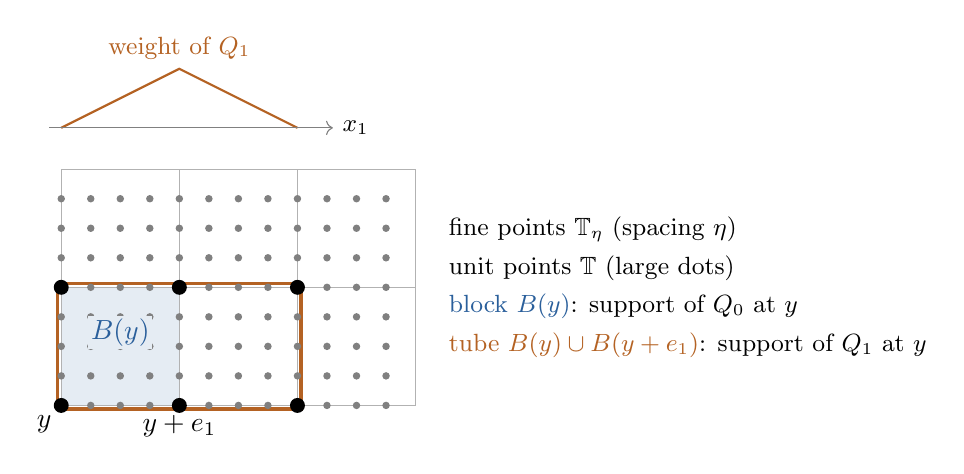
\begin{tikzpicture}[scale=1.5]
% blocks
\fill[fblue!12] (0,0) rectangle (1,1);
\draw[forange,very thick] (-0.03,-0.03) rectangle (2.03,1.03);
\foreach \i in {0,1,2,3} \draw[gray!60] (\i,0)--(\i,2);
\foreach \j in {0,1,2} \draw[gray!60] (0,\j)--(3,\j);
\foreach \i in {0,...,11} \foreach \j in {0,...,7} \fill[gray] (\i*0.25,\j*0.25) circle (0.9pt);
\foreach \i in {0,1,2} \foreach \j in {0,1} \fill[black] (\i,\j) circle (1.8pt);
\node[below left] at (0,0) {$y$};
\node[below] at (1,0) {$y+e_1$};
\node[fblue,fill=fblue!12,inner sep=1pt] at (0.5,0.62) {$B(y)$};
% weight profile of Q_1
\draw[forange,thick] (0,2.35)--(1,2.85)--(2,2.35);
\draw[gray,->] (-0.1,2.35)--(2.3,2.35) node[right,black] {\small $x_1$};
\node[forange,above] at (1,2.85) {\small weight of $Q_1$};
\node[align=left,right] at (3.2,1) {\small fine points $\Tf$ (spacing $\eta$)\\[2pt] \small unit points $\T$ (large dots)\\[2pt] \small {\color{fblue}block $B(y)$}: support of $Q_0$ at $y$\\[2pt] \small {\color{forange}tube $B(y)\cup B(y+e_1)$}: support of $Q_1$ at $y$};
\end{tikzpicture}
\caption{The two lattices for $d=2$, $N=4$. The block average $(Q_0f)(y)$ is the mean of $f$ over $B(y)$. The tube average $(Q_1f)(y)$ is the mean over $B(y)$ of the averages of $f$ along unit segments in direction $e_1$. Its weight is the triangle shown above the tube.}
\label{fig:lattices}
\end{figure}

\subsection{Fields, derivatives and the Hodge identity}

A \emph{scalar field} is a function $f:\Tf\to\R$. A \emph{gauge field} (a $1$-form) is a $d$-tuple $A=(A_1,\dots,A_d)$ of scalar fields. Here $A_\mu(x)$ is the value of $A$ on the oriented bond $(x,x+\eta e_\mu)$, and the value on the reversed bond is $-A_\mu(x)$. A $2$-form is a collection $F=(F_{\mu\nu})$ with $F_{\nu\mu}=-F_{\mu\nu}$. Here $F_{\mu\nu}(x)$ is the value on the plaquette spanned by $x$, $\eta e_\mu$ and $\eta e_\nu$. The inner products are
\[
\ip fg=\eta^d\sum_{x\in\Tf}f(x)g(x),\qquad
\ip AB=\sum_{\mu}\ip{A_\mu}{B_\mu},\qquad
\ip FE=\sum_{\mu<\nu}\ip{F_{\mu\nu}}{E_{\mu\nu}},
\]
and $\|\cdot\|$ denotes the corresponding norms. For a set $X\subset\Tf$, $\|f\|_X$ is the norm of $\one_Xf$. Unit-lattice fields are defined in the same way on $\T$, with inner product $\sum_{y\in\T}$ and no factor $\eta^d$. With these normalizations a block has volume $\eta^dN^d=1$, so constant fields have comparable norms on both lattices.

The forward and backward derivatives are
\[
(\partial_\mu f)(x)=\frac{f(x+\eta e_\mu)-f(x)}{\eta},\qquad (\partial_\mu^*f)(x)=\frac{f(x-\eta e_\mu)-f(x)}{\eta}.
\]
Then $\partial_\mu^*$ is the adjoint of $\partial_\mu$. All $\partial_\mu$ and $\partial_\nu^*$ commute with one another and with translations of $\Tf$. The exterior derivative and its adjoint are
\begin{align*}
(df)_\mu&=\partial_\mu f, & d^*A&=\sum_\mu\partial_\mu^*A_\mu,\\
(dA)_{\mu\nu}&=\partial_\mu A_\nu-\partial_\nu A_\mu, & (d^*F)_\nu&=\sum_\mu\partial_\mu^*F_{\mu\nu}.
\end{align*}
One checks directly that $d^*$ is the adjoint of $d$ and that $d(df)=0$. The (non-positive) Laplacian is $\Lap=-\sum_\mu\partial_\mu^*\partial_\mu=-d^*d$ on scalar fields. It acts on gauge fields componentwise. We use the shorthand
\[
\|\partial f\|^2=\sum_\mu\|\partial_\mu f\|^2=\ip f{-\Lap f},\qquad
\|\partial A\|^2=\sum_{\mu,\nu}\|\partial_\nu A_\mu\|^2 .
\]
Gauge fields of the form $d\lambda$ are called \emph{exact}, and those with $d^*A=0$ \emph{co-closed}.

\begin{lemma}[Hodge identities]\label{lem:hodge}
For every gauge field $A$,
\[
(d^*d+dd^*)A=-\Lap A\quad\text{(componentwise)},\qquad
\|dA\|^2+\|d^*A\|^2=\|\partial A\|^2 .
\]
Moreover $-\Lap$ is invertible on scalar fields with mean zero, and every gauge field decomposes orthogonally as $A=d\lambda+A'$ with $d^*A'=0$ and $\lambda=(-\Lap)^{-1}d^*A$. The same statements hold on the unit torus, with $\partial_\mu$ replaced by the unit difference $D_\mu g(y)=g(y+e_\mu)-g(y)$.
\end{lemma}

\begin{proof}
For the first identity,
\[
(d^*dA)_\mu=\sum_\nu\partial^*_\nu(\partial_\nu A_\mu-\partial_\mu A_\nu),\qquad (dd^*A)_\mu=\partial_\mu\sum_\nu\partial^*_\nu A_\nu,
\]
and the mixed terms cancel because $\partial_\mu$ and $\partial^*_\nu$ commute. Taking the inner product with $A$ gives the second identity. Next, $-\Lap$ is symmetric and $\ip f{-\Lap f}=\|\partial f\|^2$. This vanishes only for constant $f$ on the connected torus. Hence $-\Lap$ is invertible on the orthogonal complement of the constants. Since $d^*A$ has mean zero ($\ip1{d^*A}=\ip{d1}A=0$), $\lambda$ is well defined. Then $d^*(A-d\lambda)=d^*A+\Lap\lambda=0$, and $\ip{d\lambda}{A'}=\ip\lambda{d^*A'}=0$. The proof on $\T$ is identical.
\end{proof}

On the unit torus we write $\dl$ for the exterior derivative built from $D_\mu$, and $\dl^*$ for its adjoint, with $(D_\mu^*g)(y)=g(y-e_\mu)-g(y)$.

\subsection{Directional convolutions}

The flat block and tube averages introduced in this section are obtained by restricting products of one-dimensional averages to the unit lattice, so we introduce a convenient language for those products.

\begin{definition}
Let $\mu\in\{1,\dots,d\}$ and let $\kappa:\eta\Z\to\R$ vanish outside an interval of length at most $6$. The \emph{directional convolution} in direction $\mu$ with kernel $\kappa$ is
\[
(Kf)(x)=\sum_{s\in\eta\Z}\eta\,\kappa(s)\,f(x+se_\mu),
\]
where $x+se_\mu$ is taken modulo the torus. Products of directional convolutions in different directions are called \emph{product convolutions}.
\end{definition}

Directional convolutions commute with each other and with all translations of $\Tf$. The adjoint of $K$ has kernel $s\mapsto\kappa(-s)$. The composition of two convolutions in the same direction has kernel $(\kappa_1\star\kappa_2)(s)=\sum_t\eta\,\kappa_1(t)\kappa_2(s-t)$. Moreover $|\kappa_1\star\kappa_2|\le\|\kappa_1\|_\infty\sum_t\eta|\kappa_2(t)|$, and the support lengths add. The box averages $a_\mu$, $a^*_\mu$ and the triangle average $c_\mu$ have nonnegative kernels of mass $1$, bounded by $1$. Hence every composition of such averages, possibly composed with one further convolution whose kernel is bounded by $M$, has a kernel bounded by $1$ (respectively $M$). Its support length is the sum of the support lengths.

We use the following operators in direction $\mu$:
\begin{itemize}
\item the forward and backward \emph{box averages} $a_\mu$, $a_\mu^*$, with kernels $\one_{[0,1)}$ and $\one_{(-1,0]}$:
\[
(a_\mu f)(x)=\eta\sum_{j=0}^{N-1}f(x+j\eta e_\mu),\qquad (a_\mu^*f)(x)=\eta\sum_{j=0}^{N-1}f(x-j\eta e_\mu);
\]
\item the unit difference $D_\mu f(x)=f(x+e_\mu)-f(x)$ and the shift $(\tau_\mu f)(x)=f(x+(1-\eta)e_\mu)$;
\item the \emph{triangle average} $c_\mu=a_\mu a_\mu^*$.
\end{itemize}

\begin{lemma}[One-dimensional identities]\label{lem:1d}
For each $\mu$:
\begin{enumerate}[label=(\alph*)]
\item $D_\mu=a_\mu\partial_\mu=\partial_\mu a_\mu$ and $D_\mu^*=a_\mu^*\partial_\mu^*$;
\item $a_\mu=\tau_\mu a_\mu^*$;
\item $c_\mu$ has kernel $c(s)=(1-|s|)_+$, and $\sum_s\eta\,c(s)=1$;
\item $1-c_\mu=e_\mu\partial_\mu^*\partial_\mu$, where $e_\mu$ has a kernel $k$ with $0\le k\le\frac12$, $k(s)=0$ for $|s|\ge1$, and $|k(s)-k(s')|\le|s-s'|$. Consequently $e_\mu\partial_\mu$ is a directional convolution with kernel $k_1(s)=(k(s-\eta)-k(s))/\eta$, which satisfies $|k_1|\le1$ and vanishes outside $[-1,1+\eta]$;
\item $a_\mu-1=g_\mu\partial_\mu$, where $g_\mu$ has kernel $(1-\eta-s)\one_{[0,1)}(s)\in[0,1]$.
\end{enumerate}
\end{lemma}

\begin{proof}
All identities are between convolution operators, so it suffices to check them on $\eta\Z$, i.e.\ for functions of one variable $t$. The torus versions follow by periodization.

(a) $(a\partial f)(t)=\eta\sum_{j=0}^{N-1}\frac{f(t+(j+1)\eta)-f(t+j\eta)}{\eta}=f(t+1)-f(t)$, since $N\eta=1$. Taking adjoints gives the second identity.

(b) $(\tau a^*f)(t)=\eta\sum_{j=0}^{N-1}f(t+1-\eta-j\eta)=\eta\sum_{j'=0}^{N-1}f(t+j'\eta)$, with $j'=N-1-j$.

(c) The kernel of $aa^*$ at $s\in\eta\Z$ is $\eta\cdot\#\{t\in\eta\Z: t\in[0,1),\ s-t\in(-1,0]\}$. For $0\le s<1$ the admissible $t$ are $s,s+\eta,\dots,1-\eta$, which gives $\eta\cdot(1-s)/\eta=1-s$. The case $s<0$ is symmetric. Finally $\sum_s\eta\,c(s)=\eta\big(1+2\sum_{j=1}^{N-1}(1-j\eta)\big)=\eta(2N-1-(N-1))=1$.

(d) Let $-\Lap_1h(t)=\eta^{-2}(2h(t)-h(t+\eta)-h(t-\eta))$ denote the one-dimensional operator $\partial^*\partial$. A direct check shows $-\Lap_1(-|t|/2)=\eta^{-1}\delta_{t,0}$. Put
\[
k(t)=-\frac{|t|}2+\frac12\sum_s\eta\,|t-s|\,c(s).
\]
Then $-\Lap_1k=\eta^{-1}\delta_{\cdot,0}-c$. Hence the convolution $e$ with kernel $k$ satisfies $e\,\partial^*\partial f=(-\Lap_1k)\star f=f-cf$. If $|t|\ge1$, then $|t-s|=|t|-\operatorname{sgn}(t)s$ for all $s$ in the support of $c$. Since $c$ has mass $1$ and mean $0$, this gives $k(t)=0$. For $|t|<1$, the triangle inequality and $\sum\eta c(s)(t-s)=t$ give $k(t)\ge0$, while $\sum_s\eta|t-s|c(s)\le|t|+1$ gives $k(t)\le\frac12$. Each of the two terms defining $k$ is Lipschitz with constant $\frac12$. The formula for the kernel of $e\partial$ follows by summation by parts: $\sum_s\eta k(s)\frac{f(t+s+\eta)-f(t+s)}\eta=\sum_s\eta\frac{k(s-\eta)-k(s)}\eta f(t+s)$.

(e) $(a f)(t)-f(t)=\eta\sum_{j=0}^{N-1}\sum_{i=0}^{j-1}\eta\,\partial f(t+i\eta)=\sum_{i=0}^{N-1}\eta\,\eta(N-1-i)\,\partial f(t+i\eta)$, and $\eta(N-1-i)=1-\eta-i\eta$.
\end{proof}

\subsection{Averaging operators}

Let $\iota$ denote restriction to the unit torus, $(\iota f)(y)=f(y)$ for $y\in\T$. Its adjoint is $(\iota^*g)(x)=\eta^{-d}g(x)$ if $x\in\T$ and $0$ otherwise. Put $b=a_1a_2\cdots a_d$.

\begin{definition}[Averaging operators]\label{def:averages}
The \emph{block average} $Q_0$ and the \emph{tube averages} $Q_\mu$, $\mu=1,\dots,d$, map scalar fields on $\Tf$ to scalar fields on $\T$:
\begin{align*}
(Q_0f)(y)&=(\iota bf)(y)=\eta^d\sum_{x\in B(y)}f(x),\\
(Q_\mu f)(y)&=(\iota a_\mu bf)(y)=\eta^d\sum_{x\in B(y)}\ \eta\sum_{j=0}^{N-1}f(x+j\eta e_\mu).
\end{align*}
The \emph{gauge-field average} maps gauge fields on $\Tf$ to gauge fields on $\T$:
\[
(\bQ A)_\mu=Q_\mu A_\mu,\qquad\text{i.e.}\qquad (\bQ A)_\mu(y)=\eta^d\sum_{x\in B(y)}\eta\sum_{j=0}^{N-1}A_\mu(x+j\eta e_\mu).
\]
We write $Q_\sigma$, $\sigma\in\{0,1,\dots,d\}$, when a statement holds for all of them, and $\cK_\sigma$ for the product convolution with $Q_\sigma=\iota\cK_\sigma$ ($\cK_0=b$, $\cK_\mu=a_\mu b$).
\end{definition}

The gauge-field average is the linearization of Ba\l aban's averaging at $U=1$. In \cite[(1.11), (1.18)]{BalPropI} it is written as $(Q_kA)_b=\sum_{x\in B_k(b_-)}\eta^{d+1}A([x,x(b)])$, where $A([x,x(b)])$ is the sum of $A$ over the unit segment from $x$ to $x+e_\mu$. This is exactly $(\bQ A)_\mu(y)$. Ba\l aban's original averaging \cite[(1.8)]{BalPropI} also contains contour terms. These vanish in the axial gauge, and dropping them is the ``second point of view'' of \cite[(1.13)]{BalPropI}, which we adopt.

\begin{lemma}[Properties of the averages]\label{lem:avg}
\begin{enumerate}[label=(\alph*)]
\item $(Q_\sigma f)(y)=\eta^d\sum_xw_\sigma(y,x)f(x)$ with $0\le w_\sigma\le1$, $\eta^d\sum_xw_\sigma(y,x)=1$ and $\sum_yw_\sigma(y,x)=1$. Moreover $w_0(y,x)=\one_{B(y)}(x)$, and $w_\mu(y,\cdot)$ vanishes outside $B(y)\cup B(y+e_\mu)$.
\item $Q_\sigma1=1$ and $Q_\sigma^*1=1$. Further, $(Q_0^*g)(x)=g(y(x))$, $Q_0Q_0^*=I$, and $Q_0^*Q_0$ is the orthogonal projection onto fields that are constant on each block.
\item $|(Q_\sigma f)(y)|^2\le\eta^d\sum_xw_\sigma(y,x)|f(x)|^2$. Hence $\|Q_\sigma\|\le1$, $\|\bQ\|\le1$, and $|(Q_\sigma^* g)(x)|\le\max\{|g(y)|:w_\sigma(y,x)\neq0\}$, where at most two $y$ occur.
\item \emph{(Gauge covariance.)} $D_\mu Q_0=Q_\mu\partial_\mu$, i.e.\ $\bQ\,d=\dl Q_0$. More generally, $D_\mu Q_\sigma=\iota\,a_\mu\cK_\sigma\partial_\mu$.
\item \emph{(Curvature.)} $\dl\bQ=\bQ^{(2)}d$, where $(\bQ^{(2)}F)_{\mu\nu}=\iota\,a_\mu a_\nu b\,F_{\mu\nu}$.
\end{enumerate}
\end{lemma}

\begin{proof}
(a) For $Q_0$ this is the definition. For $Q_\mu$, the coefficient of $f(x)$ in $(Q_\mu f)(y)$ is $\eta^{d}\cdot\eta\,\#\{j\in\{0,\dots,N-1\}:x-j\eta e_\mu\in B(y)\}$. So $w_\mu(y,x)\le\eta N=1$, and $w_\mu(y,x)\neq0$ only if $x\in B(y)\cup B(y+e_\mu)$. The normalization $\eta^d\sum_xw_\sigma=Q_\sigma1=1$ is clear. The identity $\sum_yw_\sigma(y,x)=1$ is $Q_\sigma^*1=1$, which follows from $(b^*\iota^*g)(x)=g(y(x))$ and $a_\mu^*1=1$.

(b) This follows from (a). Moreover $(Q_0Q_0^*g)(y)=\eta^d\sum_{x\in B(y)}g(y)=g(y)$. Hence $Q_0^*Q_0$ is a self-adjoint idempotent, and its range consists of the block-constant fields.

(c) The first bound is Cauchy--Schwarz with the probability weights $\eta^dw_\sigma(y,\cdot)$. Summing over $y$ and using $\sum_yw_\sigma(y,x)=1$ gives $\|Q_\sigma f\|^2\le\|f\|^2$. (Below we sometimes use the weaker bound $\|Q_\sigma\|^2\le2$.) The bound on $Q_\sigma^*g$ follows from $(Q_\sigma^*g)(x)=\sum_yw_\sigma(y,x)g(y)$ and $\sum_yw_\sigma(y,x)=1$.

(d) $\iota$ commutes with unit translations, so $D_\mu Q_\sigma=\iota D_\mu\cK_\sigma=\iota\cK_\sigma a_\mu\partial_\mu$ by Lemma~\ref{lem:1d}(a). For $\sigma=0$ this equals $\iota a_\mu b\,\partial_\mu=Q_\mu\partial_\mu$.

(e) $(\dl\bQ A)_{\mu\nu}=D_\mu Q_\nu A_\nu-D_\nu Q_\mu A_\mu=\iota\,a_\nu b\,a_\mu\partial_\mu A_\nu-\iota\,a_\mu b\,a_\nu\partial_\nu A_\mu$, by (a) of Lemma~\ref{lem:1d}.
\end{proof}

Part (d) is the reason for the particular form of $\bQ$. A gauge transformation $A\mapsto A+d\lambda$ changes the average by the unit-lattice gradient of the block average of $\lambda$:
\[
\bQ(A+d\lambda)=\bQ A+\dl Q_0\lambda .
\]
In particular, the gauge transformations that preserve all averages are those with $Q_0\lambda$ constant. Modulo constants, these are those with $Q_0\lambda=0$. This is the residual gauge freedom of the variational problem, cf.\ \cite[(1.13), (1.20)]{BalPropI}.

\subsection{Restriction of product convolutions}

The averaging operators restrict a smoothed field to the unit lattice. The following estimate is used whenever we need to bound such restrictions in $\ell^2$.

\begin{lemma}[Restriction lemma]\label{lem:restriction}
Let $\cK=K_1\cdots K_d$ be a product convolution, where $K_\mu$ has a kernel bounded by $M_\mu$ and vanishing outside an interval of length $\ell_\mu\le6$. Then for every scalar field $f$,
\[
\|\iota\cK f\|_{\ell^2(\T)}\le\prod_{\mu=1}^dM_\mu(\ell_\mu+1)\ \|f\| .
\]
\end{lemma}

\begin{proof}
Write $(\cK f)(y)=\sum_t\eta^d\kappa(t)f(y+t)$ with $\kappa(t)=\prod_\mu\kappa_\mu(t_\mu)$. By Cauchy--Schwarz,
\[
|(\cK f)(y)|^2\le\Big(\sum_t\eta^d|\kappa(t)|\Big)\Big(\sum_t\eta^d|\kappa(t)|\,|f(y+t)|^2\Big).
\]
The first factor is at most $\prod_\mu M_\mu(\ell_\mu+\eta)$. Summing the second factor over $y\in\T$ gives $\sum_x\eta^d|f(x)|^2\sum_y|\kappa(x-y)|$. For fixed $x$ and $\mu$, at most $\ell_\mu+1$ integers $y_\mu$ satisfy $\kappa_\mu(x_\mu-y_\mu)\neq0$. Since $\ell_\mu+1\le7<n$, no point is counted twice on the torus. Hence $\sum_y|\kappa(x-y)|\le\prod_\mu M_\mu(\ell_\mu+1)$.
\end{proof}

When several convolutions act in the same direction, they are first merged into one directional convolution, using the composition rule above. For example, $Q_\sigma$ itself, $\iota\,a_\mu a_\nu b$, and $\iota\,b\,g_\mu$ satisfy the hypotheses with constants depending only on $d$. A shift $\tau_\mu$ composed with a convolution only moves the support of the kernel, so it does not change the bound.

\section{Poincar\'e inequalities and scalar coercivity}\label{sec:poincare}

The Laplacian $-\Lap$ on $\Tf$ has eigenvalues as small as $(2\pi/n)^2$. So it controls a field only up to modes that vary on the scale of the whole torus. The averaging term $a\|Q_\sigma f\|^2$ supplies the missing control on the unit scale. The precise statement is a Poincar\'e inequality on unit blocks, uniform in~$\eta$.

\begin{lemma}[Block Poincar\'e inequality]\label{lem:block-poincare}
For every block $B=B(y)$ and every scalar field $f$,
\[
\|f-(Q_0f)(y)\|_B^2\le\frac d2\,\eta^d\sum_{b\subset B}|\partial f(b)|^2 .
\]
Here the sum runs over all fine bonds $b=(x,x+\eta e_\mu)$ with both endpoints in $B$, and $\partial f(b)=\partial_\mu f(x)$. Consequently, for every scalar field $f$,
\begin{equation}\label{eq:poincare}
\|f-Q_0^*Q_0f\|^2\le\frac d2\|\partial f\|^2,\qquad \|f\|^2\le\frac d2\|\partial f\|^2+\|Q_0f\|^2 .
\end{equation}
\end{lemma}

\begin{proof}
Let $\bar f=(Q_0f)(y)$ be the mean of $f$ over $B$. Since $B$ has $N^d$ points and volume $1$,
\[
\|f-\bar f\|_B^2=\eta^d\sum_{x\in B}|f(x)-\bar f|^2=\frac{\eta^{2d}}2\sum_{x,x'\in B}|f(x)-f(x')|^2 .
\]
For $x,x'\in B$ we join $x'$ to $x$ by the lattice path that first moves in direction $1$ from $x'_1$ to $x_1$, then in direction $2$ from $x'_2$ to $x_2$, and so on. It stays in $B$ and has at most $d(N-1)$ steps. Then $f(x)-f(x')$ is a sum of at most $dN$ terms $\pm\eta\,\partial f(b)$, and by Cauchy--Schwarz
\[
|f(x)-f(x')|^2\le dN\eta^2\sum_{b\in\text{path}(x',x)}|\partial f(b)|^2=d\eta\sum_{b\in\text{path}(x',x)}|\partial f(b)|^2 .
\]
A bond $b=(z,z+\eta e_\mu)$ lies on the $\mu$-th segment of the path only if $z_\nu=x_\nu$ for $\nu<\mu$ and $z_\nu=x'_\nu$ for $\nu>\mu$. The remaining free coordinates are $x'_\nu$ for $\nu<\mu$, $x_\nu$ for $\nu>\mu$, and the pair $(x_\mu,x'_\mu)$. Hence at most $N^{\mu-1}\cdot N^{d-\mu}\cdot N^2=N^{d+1}$ pairs $(x,x')$ use $b$. Therefore
\[
\|f-\bar f\|_B^2\le\frac{\eta^{2d}}2\,d\eta\,N^{d+1}\sum_{b\subset B}|\partial f(b)|^2=\frac d2\,\eta^d\sum_{b\subset B}|\partial f(b)|^2,
\]
using $\eta N=1$. Summing over blocks gives the first inequality in \eqref{eq:poincare}, since bonds between different blocks only add to the right-hand side. The second follows from the orthogonal decomposition $f=(f-Q_0^*Q_0f)+Q_0^*Q_0f$ and $\|Q_0^*Q_0f\|=\|Q_0f\|$ (Lemma~\ref{lem:avg}(b)).
\end{proof}

\begin{lemma}[Comparison of averages]\label{lem:compare-avg}
For $\mu=1,\dots,d$ and every scalar field $f$,
\[
\|Q_\mu f-Q_0f\|\le 3\cdot2^d\,\|\partial_\mu f\|,\qquad
\|D_\nu Q_\sigma f\|\le 6^d\,\|\partial_\nu f\|\quad(\sigma=0,\dots,d).
\]
\end{lemma}

\begin{proof}
By Lemma~\ref{lem:1d}(e), $Q_\mu f-Q_0f=\iota\,b(a_\mu-1)f=\iota\,b\,g_\mu\,\partial_\mu f$. In direction $\mu$ the operator $a_\mu g_\mu$ has a kernel bounded by $1+\eta\le2$ and supported in an interval of length $2$. In every other direction the kernel is $\one_{[0,1)}$. Lemma~\ref{lem:restriction} gives the constant $2\cdot3\cdot2^{d-1}$. Similarly, $D_\nu Q_\sigma f=\iota\,a_\nu\cK_\sigma\partial_\nu f$ by Lemma~\ref{lem:avg}(d). This is a product of at most three box averages in each direction, with kernels bounded by $1$ and supported in intervals of length at most $3$. Lemma~\ref{lem:restriction} gives a factor at most $4$ in direction $\nu$ and at most $3$ in each other direction.
\end{proof}

\begin{corollary}[Poincar\'e inequality for all averages]\label{cor:poincare-all}
There is $C_P$, depending only on $d$, such that for every $\sigma\in\{0,\dots,d\}$ and every scalar field $f$,
\[
\|f\|^2\le C_P\big(\|\partial f\|^2+\|Q_\sigma f\|^2\big).
\]
For gauge fields, $\|A\|^2\le C_P\big(\|\partial A\|^2+\|\bQ A\|^2\big)$.
\end{corollary}

\begin{proof}
By \eqref{eq:poincare} and Lemma~\ref{lem:compare-avg}, $\|f\|^2\le\frac d2\|\partial f\|^2+2\|Q_\sigma f\|^2+2\cdot9\cdot4^d\|\partial f\|^2$. Apply this to each component $A_\mu$ with $\sigma=\mu$ and sum over $\mu$.
\end{proof}

\begin{corollary}[Scalar coercivity]\label{cor:scalar-coercive}
Let $a>0$ and $c_0=\min(1,a)/(2+2C_P)$. For every $\sigma$ and every scalar field $f$,
\[
\ip f{(-\Lap+aQ_\sigma^*Q_\sigma)f}=\|\partial f\|^2+a\|Q_\sigma f\|^2\ge c_0\big(\|f\|^2+\|\partial f\|^2\big).
\]
In particular $-\Lap+aQ_\sigma^*Q_\sigma$ is invertible, and its inverse $G_\sigma$ satisfies $0<G_\sigma\le c_0^{-1}$.
\end{corollary}

\begin{proof}
$\|\partial f\|^2+a\|Q_\sigma f\|^2\ge\min(1,a)\big(\frac12\|\partial f\|^2+\frac12(\|\partial f\|^2+\|Q_\sigma f\|^2)\big)$. Then use Corollary~\ref{cor:poincare-all} on the last bracket.
\end{proof}

This is the scalar half of Theorem~\ref{thm:A}. The next lemma is used in the gauge-field part. It concerns fields with vanishing block averages, i.e.\ generators of the residual gauge transformations.

\begin{lemma}[Fields with vanishing averages]\label{lem:kerQ0}
If $Q_0\lambda=0$, then
\[
\|\lambda\|\le\sqrt{d/2}\,\|\partial\lambda\|,\qquad \|\partial\lambda\|\le\sqrt{d/2}\,\|\Lap\lambda\| .
\]
In particular $-\Lap$ is injective on $\cN(Q_0)=\{\lambda:Q_0\lambda=0\}$.
\end{lemma}

\begin{proof}
The first inequality is \eqref{eq:poincare} with $Q_0\lambda=0$. For the second, $\|\partial\lambda\|^2=\ip\lambda{-\Lap\lambda}\le\|\lambda\|\|\Lap\lambda\|\le\sqrt{d/2}\,\|\partial\lambda\|\,\|\Lap\lambda\|$.
\end{proof}

\section{Two Fourier estimates}\label{sec:fourier}

Fourier analysis plays only a small role in this paper. Its main use is to show that averaged Green functions such as $Q_\sigma G_\sigma Q_\sigma^*$ are bounded \emph{below} uniformly in $\eta$. Upper bounds and decay are proved in position space. We also need one estimate on ``biharmonic extensions'' in the gauge-field coercivity proof.

\subsection{Fourier transform and Bloch decomposition}

The dual of the fine torus is $\Tf^*=\big((2\pi/n)\Z\big/(2\pi/\eta)\Z\big)^d$. We represent it by the momenta $p$ with $-\pi/\eta<p_\mu\le\pi/\eta$. For a scalar field $f$ we put
\[
\hat f(p)=\eta^d\sum_{x\in\Tf}e^{-\ii p\cdot x}f(x),\qquad f(x)=n^{-d}\sum_{p\in\Tf^*}e^{\ii p\cdot x}\hat f(p),\qquad \|f\|^2=n^{-d}\sum_p|\hat f(p)|^2 .
\]
On the unit torus, $\hat g(q)=\sum_{y\in\T}e^{-\ii q\cdot y}g(y)$ for $q\in\T^*$, which we represent by $-\pi<q_\mu\le\pi$, and $\|g\|^2=n^{-d}\sum_q|\hat g(q)|^2$.

Every $p\in\Tf^*$ can be written uniquely as $p=q+2\pi l$ with $q\in\T^*$ and $l\in\Z^d$. For fixed $q$ exactly $N^d$ vectors $l$ occur. This is the \emph{Bloch decomposition}.

A directional convolution with kernel $\kappa$ in direction $\mu$ acts in momentum space as multiplication by $\tilde\kappa(p_\mu)$, where $\tilde\kappa(\theta)=\sum_s\eta\,\kappa(s)e^{\ii\theta s}$. Its adjoint has symbol $\overline{\tilde\kappa}$. In particular
\[
\widehat{\partial_\mu f}(p)=\frac{e^{\ii\eta p_\mu}-1}\eta\,\hat f(p),\qquad
\widehat{-\Lap f}(p)=\hat\Lap(p)\hat f(p),\quad \hat\Lap(p)=\sum_\mu\frac4{\eta^2}\sin^2\frac{\eta p_\mu}2,
\]
and $a_\mu$ has symbol $\alpha(p_\mu)$, with
\[
\alpha(\theta)=\eta\sum_{j=0}^{N-1}e^{\ii j\eta\theta}=\eta\,\frac{e^{\ii\theta}-1}{e^{\ii\eta\theta}-1},\qquad |\alpha(\theta)|=\frac{|\sin(\theta/2)|}{N|\sin(\eta\theta/2)|}.
\]
Restriction to the unit lattice and its adjoint satisfy the \emph{Poisson summation formula}:
\begin{equation}\label{eq:poisson}
\widehat{\iota f}(q)=\sum_{l}\hat f(q+2\pi l),\qquad \widehat{\iota^*g}(p)=\hat g(q)\quad\text{for }p=q+2\pi l .
\end{equation}
The first identity follows by inserting the inversion formula for $f$ into $\sum_ye^{-\ii q\cdot y}f(y)$ and using $\sum_{y\in\T}e^{\ii(p-q)\cdot y}=n^d\one[p-q\in2\pi\Z^d]$. The second is immediate from the definition of $\iota^*$.

\begin{lemma}[Symbol bounds]\label{lem:symbols}
Let $|\theta|\le\pi/\eta$.
\begin{enumerate}[label=(\alph*)]
\item $\frac4{\pi^2}\theta^2\le\frac4{\eta^2}\sin^2\frac{\eta\theta}2\le\theta^2$. Hence $\frac4{\pi^2}|p|^2\le\hat\Lap(p)\le|p|^2$ on the fundamental domain.
\item $|\alpha(\theta)|\le1$, and $|\alpha(\theta)|\ge2/\pi$ if $|\theta|\le\pi$.
\item If $\theta=q+2\pi l$ with $|q|\le\pi$ and $l\in\Z\setminus\{0\}$, then $|\theta|\ge\pi|l|$ and $|\alpha(\theta)|\le|q|/(2|l|)$.
\end{enumerate}
\end{lemma}

\begin{proof}
(a) uses $\frac2\pi t\le\sin t\le t$ for $0\le t\le\pi/2$. (b) The first bound is the triangle inequality. For $|\theta|\le\pi$, $|\sin(\theta/2)|\ge|\theta|/\pi$ and $N|\sin(\eta\theta/2)|\le|\theta|/2$. (c) $|\theta|\ge2\pi|l|-|q|\ge\pi|l|$. Moreover $|\sin(\theta/2)|=|\sin(q/2)|\le|q|/2$, and $N|\sin(\eta\theta/2)|\ge N\frac2\pi\frac{\eta|\theta|}2=|\theta|/\pi\ge|l|$.
\end{proof}

\subsection{The lower bound}

\begin{lemma}[Fourier lower bound]\label{lem:fourier-lower}
Let $K$ be a translation-invariant operator on scalar fields of $\Tf$ with symbol $\hat K(p)\ge0$ on $\Tf^*$, and let $\cK$ be a product convolution with symbol $\kappa(p)$. Represent each $q\in\T^*$ by $-\pi<q_\mu\le\pi$; this is a point of $\Tf^*$. Then for every field $g$ on $\T$,
\[
\ip{\cK^*\iota^*g}{K\cK^*\iota^*g}\ \ge\ m\,\|g\|^2,\qquad m=\min_{q\in\T^*}\hat K(q)|\kappa(q)|^2 .
\]
\end{lemma}

\begin{proof}
By \eqref{eq:poisson}, $h=\cK^*\iota^*g$ has $\hat h(q+2\pi l)=\overline{\kappa(q+2\pi l)}\,\hat g(q)$. Therefore
\[
\ip h{Kh}=n^{-d}\sum_q|\hat g(q)|^2\sum_l\hat K(q+2\pi l)|\kappa(q+2\pi l)|^2\ \ge\ n^{-d}\sum_q|\hat g(q)|^2\,\hat K(q)|\kappa(q)|^2,
\]
where we kept only the term $l=0$. The claim follows from Parseval on $\T$.
\end{proof}

\begin{corollary}\label{cor:QKQ-lower}
For every $\sigma\in\{0,\dots,d\}$ and $a>0$,
\[
Q_\sigma(-\Lap+2a)^{-1}Q_\sigma^*\ \ge\ c_F,\qquad c_F=\Big(\frac2\pi\Big)^{2d+2}\frac1{d\pi^2+2a}.
\]
\end{corollary}

\begin{proof}
Apply Lemma~\ref{lem:fourier-lower} with $K=(-\Lap+2a)^{-1}$ and $\cK=\cK_\sigma$. The symbol of $\cK_\sigma$ is a product of at most $d+1$ factors $\alpha(p_\nu)$, each of modulus at least $2/\pi$ on $[-\pi,\pi]^d$, which contains the representatives of $\T^*$. Moreover $\hat\Lap(p)\le|p|^2\le d\pi^2$ there.
\end{proof}

\subsection{Biharmonic extensions}

The following estimate is used in Section~\ref{sec:gauge-coercivity}. Given a unit-lattice field $\omega$ with mean zero, the field $\lambda=(-\Lap)^{-2}Q_0^*\omega$ is the smoothest (in the sense of $\|\Lap\lambda\|$) fine field with prescribed block averages $Q_0\lambda$, which then have mean zero. We will see that this is exactly the gradient part of a gauge field in Ba\l aban's gauge. Its energy is controlled by the unit-lattice gradient of its averages.

\begin{lemma}[Biharmonic extensions]\label{lem:biharmonic}
There is $C_B$, depending only on $d$, with the following property. Let $\omega$ be a field on $\T$ with mean zero, and let $\lambda=(-\Lap)^{-2}Q_0^*\omega$ (the inverse taken on mean-zero fields). Then
\[
\|\partial\lambda\|\le C_B\,\|\dl Q_0\lambda\| .
\]
\end{lemma}

\begin{proof}
Let $\beta(p)=\prod_\nu\alpha(p_\nu)$ be the symbol of $b$. By \eqref{eq:poisson}, $\hat\lambda(p)=\overline{\beta(p)}\,\hat\omega(q)\,\hat\Lap(p)^{-2}$ for $p=q+2\pi l\ne0$, and $\hat\lambda(0)=0$. For $j\in\{2,3\}$ and $q\in\T^*\setminus\{0\}$ put $S_j(q)=\sum_l|\beta(q+2\pi l)|^2\hat\Lap(q+2\pi l)^{-j}$. Then
\[
\|\partial\lambda\|^2=\ip\lambda{-\Lap\lambda}=n^{-d}\sum_{q\ne0}|\hat\omega(q)|^2S_3(q).
\]
The term $q=0$ is absent, because $\hat\omega(0)=0$, and because for $l\ne0$ some factor $\alpha(2\pi l_\nu)$ vanishes. Similarly, $g=Q_0\lambda=\iota b\lambda$ has $\hat g(q)=\sum_l\beta(q+2\pi l)\hat\lambda(q+2\pi l)=\hat\omega(q)S_2(q)$, and
\[
\|\dl g\|^2=n^{-d}\sum_{q\ne0}\hat\Lap_1(q)\,S_2(q)^2\,|\hat\omega(q)|^2,\qquad \hat\Lap_1(q)=\sum_\nu4\sin^2\frac{q_\nu}2 .
\]
It therefore suffices to show $S_3(q)\le C_B^2\hat\Lap_1(q)S_2(q)^2$ for $q\in[-\pi,\pi]^d\setminus\{0\}$.

By Lemma~\ref{lem:symbols}, keeping only the term $l=0$ in $S_2$, we get $S_2(q)\ge(2/\pi)^{2d}|q|^{-4}$, and $\hat\Lap_1(q)\ge\frac4{\pi^2}|q|^2$. Hence
\[
\hat\Lap_1(q)S_2(q)^2\ge\frac4{\pi^2}\Big(\frac2\pi\Big)^{4d}|q|^{-6}.
\]
In $S_3$, the term $l=0$ is at most $(\pi/2)^6|q|^{-6}$. For $l\ne0$, Lemma~\ref{lem:symbols}(a),(c) gives $\hat\Lap(q+2\pi l)\ge\frac4{\pi^2}|q+2\pi l|^2\ge4|l|^2\ge4$ and $|\beta(q+2\pi l)|^2\le\prod_{\nu:\,l_\nu\ne0}\frac{\pi^2}{4l_\nu^2}$. Hence
\[
\sum_{l\ne0}\frac{|\beta(q+2\pi l)|^2}{\hat\Lap(q+2\pi l)^3}\le\frac1{64}\prod_{\nu=1}^d\Big(1+2\sum_{m\ge1}\frac{\pi^2}{4m^2}\Big)=\frac1{64}\Big(1+\frac{\pi^4}{12}\Big)^d .
\]
Since $|q|^2\le d\pi^2$, this constant is at most $\frac1{64}(1+\pi^4/12)^d(d\pi^2)^3|q|^{-6}$, and the lemma follows.
\end{proof}

\section{Operators with exponential decay and the Combes--Thomas method}\label{sec:decay}

Exponential decay will first be established in $L^2$, between unit blocks. This section develops the bookkeeping for this notion and the basic mechanism that produces it: if $K$ is coercive and conjugation by $e^{\alpha\rho}$ changes $K$ only by $O(\alpha)$, then $K^{-1}$ decays exponentially.

\subsection{Block decay}

We work with four kinds of field spaces: scalar fields and gauge fields on $\Tf$, and scalar fields and gauge fields on $\T$. On each of them we have the \emph{localization projections} $\one_y$, $y\in\T$. On the fine lattice, $\one_y$ is multiplication by the indicator of $B(y)$ (for gauge fields: of the bonds $(x,x+\eta e_\mu)$ with $x\in B(y)$). On the unit lattice, $\one_y$ keeps the value(s) at $y$. In all cases $\sum_y\one_y=I$.

\begin{definition}\label{def:decay}
A linear operator $K$ between two such spaces has \emph{decay $(C,\gamma)$} if
\[
\|\one_yK\one_{y'}\|\le Ce^{-\gamma|y-y'|}\qquad\text{for all }y,y'\in\T .
\]
\end{definition}

For operators between unit-lattice spaces, $\|\one_yK\one_{y'}\|$ is the absolute value (or matrix norm) of the kernel $K(y,y')$, so decay is a pointwise kernel bound. We put
\[
S_\gamma=\sum_{z\in\Z^d}e^{-\gamma|z|}.
\]
Then $\sum_{y'\in\T}e^{-\gamma|y-y'|}\le S_\gamma$ for every $y$, uniformly in $n$, because distinct $y'$ have distinct nearest representatives of $y'-y$ in $\Z^d$.

\begin{lemma}[Calculus of decay]\label{lem:decay-calculus}
\begin{enumerate}[label=(\alph*)]
\item If $K$ has decay $(C,\gamma)$, then $\|K\|\le CS_\gamma$.
\item If $K_1$ and $K_2$ have decay $(C_1,\gamma)$ and $(C_2,\gamma)$, then $K_1K_2$ has decay $(C_1C_2S_{\gamma/2},\gamma/2)$.
\item If $K$ has decay $(C,\gamma)$ then $K^*$ has decay $(C,\gamma)$. Sums behave in the obvious way, and decay $(C,\gamma)$ implies decay $(C,\gamma')$ for $\gamma'\le\gamma$.
\item If $\one_yK\one_{y'}=0$ for $|y-y'|>r$ and $\|K\|\le M$, then $K$ has decay $(Me^{\gamma r},\gamma)$ for every $\gamma>0$.
\end{enumerate}
\end{lemma}

\begin{proof}
(a) $\|\one_yKf\|\le\sum_{y'}Ce^{-\gamma|y-y'|}\|\one_{y'}f\|$. The matrix $(e^{-\gamma|y-y'|})$ has row and column sums at most $S_\gamma$, so by the Schur test it defines an operator on $\ell^2(\T)$ of norm at most $S_\gamma$. Hence $\|Kf\|^2=\sum_y\|\one_yKf\|^2\le C^2S_\gamma^2\sum_{y'}\|\one_{y'}f\|^2$.

(b) $\one_yK_1K_2\one_{y'}=\sum_{y''}\one_yK_1\one_{y''}K_2\one_{y'}$. By the triangle inequality $|y-y''|+|y''-y'|\ge\frac12|y-y'|+\frac12|y-y''|$, so the norm is at most $C_1C_2e^{-\gamma|y-y'|/2}\sum_{y''}e^{-\gamma|y-y''|/2}$.

(c) and (d) are immediate.
\end{proof}

\subsection{Conjugation by exponential weights}

A function $\rho:\Tf\to\R$ is \emph{$1$-Lipschitz} if $|\rho(x)-\rho(x')|\le|x-x'|$ for all $x,x'$. A typical example is $\rho(x)=\operatorname{dist}(x,B(y'))$, the torus distance to a block. For $\alpha\in\R$, multiplication by $e^{\alpha\rho}$ acts on all four field spaces. On unit-lattice fields it multiplies the value at $y$ by $e^{\alpha\rho(y)}$, which is consistent because $\T\subset\Tf$. For an operator $K$ we write
\[
K_\alpha=e^{\alpha\rho}Ke^{-\alpha\rho}.
\]
Then $(K_1K_2)_\alpha=(K_1)_\alpha(K_2)_\alpha$, $(K^*)_\alpha=(K_{-\alpha})^*$, and $(K^{-1})_\alpha=(K_\alpha)^{-1}$. Since $\iota$ commutes with multiplication operators, $(\iota)_\alpha=\iota$.

\begin{lemma}[Conjugation of decaying operators]\label{lem:conjugation}
Let $K$ have decay $(C,\gamma)$ and let $\rho$ be $1$-Lipschitz. For $|\alpha|\le\gamma/2$,
\[
\|K_\alpha-K\|\le C\,c_1(\gamma)\,|\alpha|,\qquad c_1(\gamma)=e^{\gamma\sqrt d}\big(2\sqrt d+4/\gamma\big)S_{\gamma/4}.
\]
\end{lemma}

\begin{proof}
Fix $y,y'$, put $X=\one_yK\one_{y'}$, and write $e^{\alpha\rho}=e^{\alpha\rho(y)}E$ on the support of $\one_y$. Here $E$ is multiplication by $e^{\alpha(\rho-\rho(y))}$. Since points of $B(y)$ are within distance $\sqrt d$ of $y$, $\|E-1\|\le|\alpha|\sqrt d\,e^{|\alpha|\sqrt d}$ and $\|E\|\le e^{|\alpha|\sqrt d}$. Define $E'$ similarly at $y'$. Then $\one_y(K_\alpha-K)\one_{y'}=sEXE'^{-1}-X$ with $s=e^{\alpha(\rho(y)-\rho(y'))}$. Since $|s-1|\le|\alpha||y-y'|e^{|\alpha||y-y'|}$, the decomposition
\[
sEXE'^{-1}-X=(s-1)EXE'^{-1}+(E-1)XE'^{-1}+X(E'^{-1}-1)
\]
gives
\[
\|\one_y(K_\alpha-K)\one_{y'}\|\le C|\alpha|\,e^{2|\alpha|\sqrt d}\big(|y-y'|+2\sqrt d\big)e^{-(\gamma-|\alpha|)|y-y'|}.
\]
For $|\alpha|\le\gamma/2$ we have $e^{2|\alpha|\sqrt d}\le e^{\gamma\sqrt d}$ and $(t+2\sqrt d)e^{-\gamma t/2}\le(2\sqrt d+4/\gamma)e^{-\gamma t/4}$. Hence $K_\alpha-K$ has decay $(C|\alpha|e^{\gamma\sqrt d}(2\sqrt d+4/\gamma),\gamma/4)$, and Lemma~\ref{lem:decay-calculus}(a) concludes.
\end{proof}

\begin{lemma}[Conjugated derivatives]\label{lem:conj-derivative}
Let $\rho$ be $1$-Lipschitz and $|\alpha|\le1$. Then $(\partial_\mu)_\alpha=\partial_\mu+Y$ and $(\partial_\mu^*)_\alpha=\partial_\mu^*+Y'$, where $Y,Y'$ are operators of norm at most $e|\alpha|$. On gauge fields the same holds componentwise.
\end{lemma}

\begin{proof}
$(e^{\alpha\rho}\partial_\mu e^{-\alpha\rho}u)(x)=\partial_\mu u(x)+\eta^{-1}\big(e^{\alpha(\rho(x)-\rho(x+\eta e_\mu))}-1\big)u(x+\eta e_\mu)$. Moreover $|e^t-1|\le|t|e^{|t|}$ with $|t|\le|\alpha|\eta$. The computation for $\partial_\mu^*$ is the same.
\end{proof}

\subsection{The Combes--Thomas method}

We give two versions. The first is for bounded operators, typically on the unit lattice. The second is for fine-lattice operators containing $-\Lap$, whose norm is of order $\eta^{-2}$.

\begin{lemma}[Combes--Thomas, bounded version]\label{lem:CT-bounded}
Let $K$ act on one of the four field spaces, have decay $(C,\gamma)$, and satisfy $\ip f{Kf}\ge c\|f\|^2$ for all (real) fields $f$. Put $\gamma'=\min\{\gamma/2,\ c/(2Cc_1(\gamma))\}$. Then $K$ is invertible and $K^{-1}$ has decay $(2c^{-1}e^{2\gamma'\sqrt d},\gamma')$.
\end{lemma}

\begin{proof}
Fix $y'$, let $\rho(x)=\operatorname{dist}(x,B(y'))$ and $\alpha=\gamma'$. By Lemma~\ref{lem:conjugation}, $\ip f{K_\alpha f}\ge c\|f\|^2-\frac c2\|f\|^2$. Hence $K_\alpha$ is invertible with $\|K_\alpha^{-1}\|\le2/c$. Here we use that in finite dimensions $\ip f{Xf}\ge\delta\|f\|^2$ implies $\|Xf\|\ge\delta\|f\|$. Now $K^{-1}=e^{-\alpha\rho}K_\alpha^{-1}e^{\alpha\rho}$. On the support of $\one_{y'}$ we have $\rho=0$. On the support of $\one_y$ we have $\rho\ge|y-y'|-2\sqrt d$. Therefore $\|\one_yK^{-1}\one_{y'}\|\le e^{-\alpha(|y-y'|-2\sqrt d)}\,2/c$.
\end{proof}

\begin{lemma}[Neumann series]\label{lem:neumann}
Let $\mathfrak N$ have decay $(C,\gamma)$ and $\|\mathfrak N\|\le\theta<1$. Then $(I+\mathfrak N)^{-1}$ has decay $(2(1-\theta)^{-1}e^{2\gamma'\sqrt d},\gamma')$ with $\gamma'=\min\{\gamma/2,(1-\theta)/(2Cc_1(\gamma))\}$.
\end{lemma}

\begin{proof}
As above, with $\|\mathfrak N_\alpha\|\le\theta+(1-\theta)/2$, so that $\|(I+\mathfrak N_\alpha)^{-1}\|\le2/(1-\theta)$.
\end{proof}

This lemma is the form in which exponential decay is used in the variational problem, cf.\ \cite[(68)--(71)]{BalVar}.

For the fine-lattice operators we write $\partial$ for the collection $(\partial_\mu)_\mu$ acting on scalar fields, or componentwise on gauge fields, and $\partial^*$ for its adjoint.

\begin{lemma}[Combes--Thomas, form version]\label{lem:CT-form}
Let $\mathfrak A$ act on scalar or gauge fields on $\Tf$. Suppose that:
\begin{enumerate}[label=(\roman*)]
\item $\ip u{\mathfrak Au}\ge c\,(\|u\|^2+\|\partial u\|^2)$ for all $u$;
\item there are $C_1,\alpha_1>0$ such that for every $1$-Lipschitz $\rho$, every $|\alpha|\le\alpha_1$ and every $u$,
\[
|\ip u{(\mathfrak A_\alpha-\mathfrak A)u}|\le C_1|\alpha|\,(\|u\|^2+\|\partial u\|^2).
\]
\end{enumerate}
Let $\gamma_0=\min\{\alpha_1,1/3,c/(2C_1)\}$. Then the four operators $\mathfrak A^{-1}$, $\partial\mathfrak A^{-1}$, $\mathfrak A^{-1}\partial^*$ and $\partial\mathfrak A^{-1}\partial^*$ have decay $(C_0,\gamma_0)$, with $C_0=2(1+\sqrt d)^2c^{-1}e^{2\gamma_0\sqrt d}$.
\end{lemma}

\begin{proof}
Let $|\alpha|\le\gamma_0$. By (i) and (ii), $\ip u{\mathfrak A_\alpha u}\ge\frac c2(\|u\|^2+\|\partial u\|^2)$, so $\mathfrak A_\alpha$ is invertible. Let $u=\mathfrak A_\alpha^{-1}h$. Then $\frac c2(\|u\|^2+\|\partial u\|^2)\le\|u\|\|h\|$. This gives $\|u\|\le\frac2c\|h\|$ and then $\|\partial u\|^2\le\frac2c\|u\|\|h\|\le\frac4{c^2}\|h\|^2$. If instead $h=\partial^*g$, then $\frac c2(\|u\|^2+\|\partial u\|^2)\le\ip{\partial u}g\le\|\partial u\|\|g\|$, which gives $\|\partial u\|\le\frac2c\|g\|$ and $\|u\|\le\frac2c\|g\|$. Thus
\[
\|\mathfrak A_\alpha^{-1}\|,\ \|\partial\mathfrak A_\alpha^{-1}\|,\ \|\mathfrak A_\alpha^{-1}\partial^*\|,\ \|\partial\mathfrak A_\alpha^{-1}\partial^*\|\le\frac2c .
\]
Now fix $y'$, let $\rho=\operatorname{dist}(\cdot,B(y'))$ and $\alpha=\gamma_0$. By Lemma~\ref{lem:conj-derivative}, $\partial e^{-\alpha\rho}=e^{-\alpha\rho}(\partial+Y)$ and $e^{\alpha\rho}\partial^*=(\partial^*+Y'^{*})e^{\alpha\rho}$, where $Y'$ comes from $(\partial)_{-\alpha}$. Here $Y=(Y_\mu)_\mu$ and $Y'$ consist of $d$ operators, each of norm at most $e\alpha$ by Lemma~\ref{lem:conj-derivative}, so $\|Y\|,\|Y'\|\le\sqrt d\,e\alpha$. Hence, for instance,
\[
\one_y\partial\mathfrak A^{-1}\partial^*\one_{y'}=\one_ye^{-\alpha\rho}(\partial+Y)\mathfrak A_\alpha^{-1}(\partial^*+Y'^*)\one_{y'},
\]
where we used $e^{\alpha\rho}\one_{y'}=\one_{y'}$. The middle operator has norm at most $\frac2c(1+\sqrt d\,e\alpha)^2\le\frac2c(1+\sqrt d)^2$, because $e\alpha\le1$, and $\|\one_ye^{-\alpha\rho}\|\le e^{-\alpha(|y-y'|-2\sqrt d)}$. The other three operators are treated in the same way.
\end{proof}

The hypothesis (ii) is verified with the help of the following observation.

\begin{lemma}[Conjugation of quadratic forms]\label{lem:conj-forms}
Let $X=X_0-Z$, where $X_0=\sum_jc_j\,\partial^{(*)}_{\mu_j}$ is a finite linear combination of the operators $\partial_\mu$, $\partial^*_\mu$ (acting componentwise on scalar or gauge fields, with values in the appropriate form degree) with scalar coefficients $\sum_j|c_j|\le M$, and $Z$ is bounded with $\|Z\|\le M$ and $\|Z_\alpha-Z\|\le M|\alpha|$ for $|\alpha|\le\alpha_1\le1$. Then for $|\alpha|\le\alpha_1$,
\[
|\ip u{((X^*X)_\alpha-X^*X)u}|\le C_M|\alpha|\,(\|u\|^2+\|\partial u\|^2),
\]
with $C_M$ depending only on $M$ and $d$.
\end{lemma}

\begin{proof}
By Lemma~\ref{lem:conj-derivative}, applied to each term of $X_0$, $X_\alpha=X+W_\alpha$ with $\|W_\alpha\|\le(eM+M)|\alpha|$. Also $\|X_0u\|\le M\|\partial u\|$. Since $(X^*X)_\alpha=(X_{-\alpha})^*X_\alpha$,
\[
\ip u{((X^*X)_\alpha-X^*X)u}=\ip{W_{-\alpha}u}{Xu}+\ip{Xu}{W_\alpha u}+\ip{W_{-\alpha}u}{W_\alpha u}.
\]
Finally, $\|Xu\|\le M(\|\partial u\|+\|u\|)$.
\end{proof}

\section{Local regularity on the fine lattice}\label{sec:regularity}

The Combes--Thomas method gives $L^2$ bounds between unit blocks. To obtain bounds on values, derivatives and H\"older quotients that are uniform in $\eta$, we use an interior regularity estimate for the lattice Laplacian. This is the lattice analogue of the classical fact that a solution of $-\Lap u=F$ with bounded $F$ is $C^{1,\alpha}$ in the interior for every $\alpha<1$. In this section $d\ge3$.

\subsection{The Green function of the fine lattice}

Let $g_1$ be the Green function of $-\Lap$ on the infinite unit lattice $\Z^d$:
\[
g_1(x)=\frac1{(2\pi)^d}\int_{[-\pi,\pi]^d}\frac{e^{\ii p\cdot x}}{\sum_\mu4\sin^2(p_\mu/2)}\,dp ,
\]
which is well defined for $d\ge3$ and satisfies $-\Lap g_1=\delta_0$. On $\eta\Z^d$ put $g_\eta(x)=\eta^{2-d}g_1(x/\eta)$. Then the convolution
\[
(\cG h)(x)=\sum_{x'\in\eta\Z^d}\eta^d\,g_\eta(x-x')\,h(x')
\]
satisfies $-\Lap\cG h=h$ and $\cG(-\Lap h)=h$ for every finitely supported $h$ on $\eta\Z^d$. For the second identity, sum by parts. Since $\cG$ is a convolution, it commutes with all lattice derivatives: $\partial_\mu\cG h=(\partial_\mu g_\eta)\star h$, and similarly for $\partial^*_\mu$.

\begin{proposition}[Decay of derivatives]\label{prop:green-eta}
For every word $\partial^\beta$ of length $|\beta|\le3$ in the operators $\partial_\mu,\partial^*_\mu$,
\[
|\partial^\beta g_\eta(x)|\le C_\beta\,(|x|+\eta)^{2-d-|\beta|},\qquad x\in\eta\Z^d,
\]
with $C_\beta$ depending only on $d$ and $\beta$.
\end{proposition}

\begin{proof}
By scaling, $\partial^\beta g_\eta(x)=\eta^{2-d-|\beta|}(\nabla^\beta g_1)(x/\eta)$, where $\nabla^\beta$ is the corresponding word of unit-lattice differences. By Theorem~\ref{thm:green-unit} in Appendix~\ref{app:green}, $|\nabla^\beta g_1(z)|\le C_\beta(1+|z|)^{2-d-|\beta|}$.
\end{proof}

We also need two elementary lattice sums.

\begin{lemma}[Lattice sums]\label{lem:lattice-sums}
Let $x\in\eta\Z^d$ and $R\ge\eta$.
\begin{enumerate}[label=(\alph*)]
\item For $0\le s<d$: $\sum_{|x'-x|\le R}\eta^d(|x-x'|+\eta)^{-s}\le C_{d,s}R^{d-s}$.
\item For $\sqrt d\,\eta\le r\le R$: $\sum_{r<|x'-x|\le R}\eta^d|x-x'|^{-d}\le C_d\,(1+\log(R/r))$.
\item For $s>d$ and $r\ge\sqrt d\,\eta$: $\sum_{|x'-x|>r}\eta^d|x-x'|^{-s}\le C_{d,s}\,r^{d-s}$.
\end{enumerate}
\end{lemma}

\begin{proof}
Let $W(x')=x'+[-\eta/2,\eta/2)^d$. For $z\in W(x')$ we have $|z-x|+\eta\le(1+\sqrt d)(|x-x'|+\eta)$. Hence each term in (a) is at most $(1+\sqrt d)^s\int_{W(x')}(|z-x|+\eta)^{-s}dz$. The cubes $W(x')$ are disjoint and contained in the ball of radius $R+\sqrt d\eta\le(1+\sqrt d)R$, which gives (a). In (b), $|x-x'|>r\ge\sqrt d\eta$ implies $\frac12|x-x'|\le|z-x|\le\frac32|x-x'|$ for $z\in W(x')$. Hence the sum is at most $(3/2)^d\int_{r/2\le|z-x|\le3R/2}|z-x|^{-d}dz=(3/2)^d|S^{d-1}|\log(3R/r)$. The same comparison gives (c).
\end{proof}

\subsection{The regularity estimate}

For $z\in\R^d$ and $r>0$ let $\Lam_r=\{x\in\Tf:|x-z|_\infty\le r\}$. Since $n\ge8$, $\Lam_3$ can be identified with a subset of $\eta\Z^d$.

\begin{theorem}[Interior regularity]\label{thm:local-regularity}
Let $d\ge3$ and $\alpha\in(0,1)$. There is $C$, depending only on $d$ and $\alpha$, such that the following holds for every lattice spacing $\eta\le1$, in particular $\eta=1/N$ with $N\ge1$, and all $z$; for a spacing not of the form $1/N$, $\Lam_r$ is the set of $x\in\eta\Z^d$ with $|x-z|_\infty\le r$. Let $u,F:\Lam_3\to\R$ and $g=(g_\mu):\Lam_3\to\R^d$ satisfy
\[
-\Lap u=F+\sum_\mu\partial^*_\mu g_\mu\qquad\text{at every point of }\Lam_2 .
\]
\begin{enumerate}[label=(\alph*)]
\item If $g=0$: $\ |u|_{\Lam_1}+|\partial u|_{\Lam_1}+\Hol{\partial u}{\Lam_1}\le C\big(|F|_{\Lam_2}+\|u\|_{\Lam_2}\big)$.
\item In general: $\ |u|_{\Lam_1}+\Hol{u}{\Lam_1}\le C\big(|F|_{\Lam_2}+|g|_{\Lam_3}+\|u\|_{\Lam_2}\big)$.
\item If $g=0$: $\ \max_{\mu,\nu}|\partial_\mu\partial_\nu u|_{\Lam_1}\le C\big(|F|_{\Lam_2}+\Hol{F}{\Lam_2}+\|u\|_{\Lam_2}\big)$.
\item (Divergence form with H\"older data.) $\ |u|_{\Lam_1}+|\partial u|_{\Lam_1}+\Hol{\partial u}{\Lam_1}\le C\big(|F|_{\Lam_2}+|g|_{\Lam_3}+\Hol g{\Lam_3}+\|u\|_{\Lam_2}\big)$.
\end{enumerate}
\end{theorem}

\begin{figure}[t]
\centering
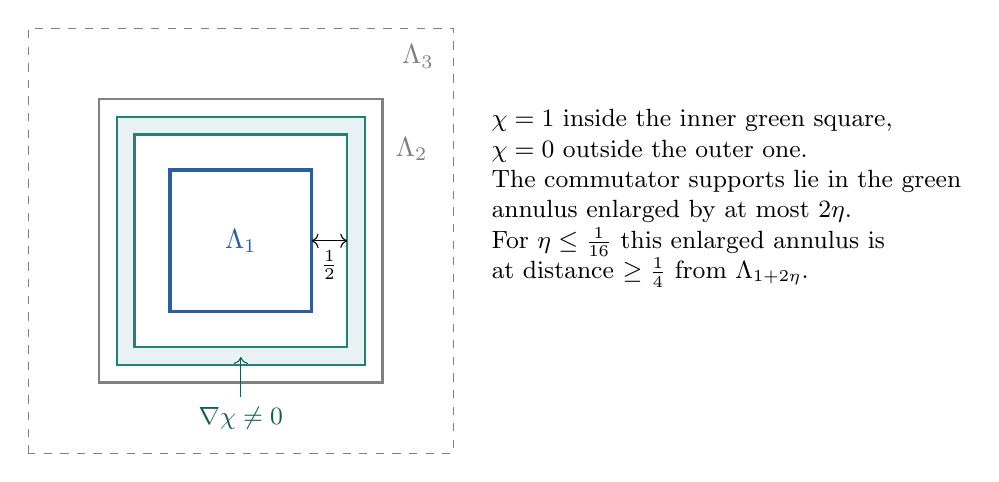
\begin{tikzpicture}[scale=0.9]
\fill[fgreen!10] (-1.75,-1.75) rectangle (1.75,1.75);
\fill[white] (-1.5,-1.5) rectangle (1.5,1.5);
\draw[fblue,very thick] (-1,-1) rectangle (1,1);
\draw[gray,thick] (-2,-2) rectangle (2,2);
\draw[gray,dashed] (-3,-3) rectangle (3,3);
\draw[fgreen,thick] (-1.5,-1.5) rectangle (1.5,1.5);
\draw[fgreen,thick] (-1.75,-1.75) rectangle (1.75,1.75);
\node[fblue] at (0,0) {$\Lam_1$};
\node[gray] at (2.5,2.6) {$\Lam_3$};
\node[gray,anchor=west] at (2.05,1.3) {$\Lam_2$};
\node[fgreen!70!black,font=\small] (lab) at (0,-2.5) {$\nabla\chi\ne0$};\draw[fgreen!70!black,->] (lab.north)--(0,-1.64);
\draw[<->] (1,0)--(1.5,0) node[midway,below,font=\small] {$\tfrac12$};
\node[align=left,anchor=west,font=\small] at (3.4,0.6) {$\chi=1$ inside the inner green square,\\ $\chi=0$ outside the outer one.\\ The commutator supports lie in the green\\ annulus enlarged by at most $2\eta$.\\ For $\eta\le\frac1{16}$ this enlarged annulus is\\ at distance $\ge\frac14$ from $\Lam_{1+2\eta}$.};
\end{tikzpicture}
\caption{Geometry of the proof of Theorem~\ref{thm:local-regularity}.}
\label{fig:cutoff}
\end{figure}

\begin{proof}
\emph{Step 0: coarse lattices.} Let $\eta>\frac1{16}$ (for $\eta=1/N$: $N<16$). Then $|u(x)|\le\eta^{-d/2}\|u\|_{\Lam_2}\le16^{d/2}\|u\|_{\Lam_2}$ for $x\in\Lam_2$, and $\Hol{v}{X}\le2\eta^{-\alpha}|v|_X$. A first difference at a point of $\Lam_1$ involves only points of $\Lam_{1+\eta}\subset\Lam_2$ and costs a factor at most $2/\eta\le32$. This proves (a), (b) and (d). For (c) with $\eta\le\frac12$, a second difference at a point of $\Lam_1$ involves only points of $\Lam_{1+2\eta}\subset\Lam_2$ and costs a factor at most $4/\eta^2$. If $\eta>\frac12$ (for $\eta=1/N$: $N=1$), the difference $\partial_\mu\partial_\mu u(x)$ involves $u(x+2\eta e_\mu)$, which may lie outside $\Lam_2$. Put $v=x+\eta e_\mu$. Since $g=0$ in (c), the equation at $v\in\Lam_2$ gives
\[
\eta^2\partial_\mu\partial_\mu u(x)=(2d-2)\,u(v)-\sum_{\nu\ne\mu}\big(u(v+\eta e_\nu)+u(v-\eta e_\nu)\big)-\eta^2F(v),
\]
and all points on the right lie in $\Lam_2$. The mixed differences $\partial_\mu\partial_\nu u(x)$, $\mu\ne\nu$, involve only points of $\Lam_2$. We assume $\eta\le\frac1{16}$ from now on.

\emph{Step 1: cutoff.} Fix $\chi\in C^\infty(\R^d)$ with $0\le\chi\le1$, $\chi=1$ on $\{|x-z|_\infty\le\frac32\}$ and $\chi=0$ on $\{|x-z|_\infty\ge\frac74\}$. Its lattice differences up to order three are bounded by constants depending only on $d$. Let $v=\chi u$, extended by zero to $\eta\Z^d$. Write $S_\mu u(x)=u(x+\eta e_\mu)$. The discrete Leibniz rules
\[
\partial_\mu(\chi u)=\chi\,\partial_\mu u+(\partial_\mu\chi)S_\mu u,\qquad
\partial_\mu^*(\varphi w)=\varphi\,\partial^*_\mu w+(\partial^*_\mu\varphi)S_\mu^{-1}w,
\]
and $S_\mu^{-1}\partial_\mu u=-\partial^*_\mu u$ give, after a short computation,
\begin{equation}\label{eq:commutator}
-\Lap(\chi u)=\chi(-\Lap u)+\sum_\mu\big(\partial^*_\mu m_\mu+n_\mu\big),\qquad
\begin{aligned}
m_\mu&=(\partial_\mu\chi)S_\mu u-(\partial^*_\mu\chi)u,\\
n_\mu&=(\partial^*_\mu\partial^*_\mu\chi)S_\mu^{-1}u .
\end{aligned}
\end{equation}
The functions $m_\mu$, $n_\mu$ vanish outside the annulus $A=\Lam_{7/4+2\eta}\setminus\Lam_{3/2-2\eta}$, where the differences of $\chi$ (up to second order, involving points at distance up to $2\eta$) can be non-zero. They involve $u$ only at points of $\Lam_2$, and $|m_\mu|+|n_\mu|\le C|u|$ at neighbouring points. Similarly $\chi\,\partial^*_\mu g_\mu=\partial^*_\mu(\chi g_\mu)-(\partial^*_\mu\chi)S_\mu^{-1}g_\mu$. Hence
\[
-\Lap v=\Phi_1+\Phi_2+\sum_\mu\partial^*_\mu(\chi g_\mu+m_\mu),\qquad
\Phi_1=\chi F-\sum_\mu(\partial^*_\mu\chi)S^{-1}_\mu g_\mu,\quad \Phi_2=\sum_\mu n_\mu .
\]
All terms vanish outside $\Lam_2$. Since $v$ has finite support,
\begin{equation}\label{eq:rep}
v=\cG\Phi_1+\cG\Phi_2+\sum_\mu(\partial^*_\mu g_\eta)\star(\chi g_\mu)+\sum_\mu(\partial^*_\mu g_\eta)\star m_\mu .
\end{equation}
For $x\in\Lam_{1+2\eta}$ we have $v(x)=u(x)$. So $u$, $\partial u$ and $\partial\partial u$ on $\Lam_1$ can be computed from \eqref{eq:rep}.

\emph{Step 2: the terms supported in the annulus.} Points of $\Lam_{1+2\eta}$ have distance at least $\frac12-4\eta\ge\frac14$ from $A$. By Proposition~\ref{prop:green-eta}, every derivative of order at most three of $g_\eta$ is bounded by a constant on $\{|x|\ge\frac14\}$. Therefore, for $x\in\Lam_{1+2\eta}$ and $|\beta|\le2$,
\[
|\partial^\beta\cG\Phi_2(x)|+\sum_\mu|\partial^\beta(\partial^*_\mu g_\eta)\star m_\mu(x)|\le C\sum_{x'\in A}\eta^d\Big(|\Phi_2(x')|+\sum_\mu|m_\mu(x')|\Big)\le C\|u\|_{\Lam_2},
\]
by Cauchy--Schwarz. For $|\beta|\le1$ the derivatives of order one more are also bounded (they involve at most three derivatives of $g_\eta$), so these terms and their first derivatives are Lipschitz on $\Lam_1$; for (c) only the sup bounds with $|\beta|=2$ are needed. A Lipschitz function on $\Lam_1$ is H\"older: join $x,x'$ by a monotone lattice path inside $\Lam_1$, of length at most $\sqrt d|x-x'|\le2d$.

\emph{Step 3: the near terms in (a) and (b).} Here $\Phi_1$ and $\chi g$ are bounded by $C(|F|_{\Lam_2}+|g|_{\Lam_3})$ and supported in $\Lam_2$. By Lemma~\ref{lem:lattice-sums}(a) with $s=d-2$ and $s=d-1$, for $x\in\Lam_{1+2\eta}$,
\[
|\cG\Phi_1(x)|+|\partial\cG\Phi_1(x)|+|(\partial^*g_\eta)\star(\chi g)(x)|\le C(|F|_{\Lam_2}+|g|_{\Lam_3}).
\]
This proves the sup bounds in (a) and (b), and shows that $\cG\Phi_1$ is Lipschitz on $\Lam_1$. It remains to estimate the H\"older quotient of a convolution $k\star h$ with $|h|\le M$ supported in $\Lam_2$. Here $k=\partial_\mu g_\eta$ in (a), and $k=\partial^*_\mu g_\eta$ in (b). In both cases $|k(y)|\le C(|y|+\eta)^{1-d}$, and every first difference of $k$ is bounded by $C(|y|+\eta)^{-d}$. Let $x,x'\in\Lam_1$, $\delta=|x-x'|\ge\eta$. Split the sum over $x''$ at $|x-x''|=4\sqrt d\,\delta$. On the near part, by Lemma~\ref{lem:lattice-sums}(a) with $s=d-1$ (note $|x'-x''|\le(4\sqrt d+1)\delta$),
\[
\sum_{|x-x''|\le4\sqrt d\delta}\eta^d\big(|k(x-x'')|+|k(x'-x'')|\big)\le C\delta ,
\]
On the far part we join $x$ to $x'$ by a monotone lattice path of at most $\sqrt d\delta/\eta$ steps. Every point $w$ of the path, and its neighbours, satisfies $|w-x''|\ge\frac12|x-x''|$. Hence $|k(x-x'')-k(x'-x'')|\le C\sqrt d\,\delta\,|x-x''|^{-d}$, and by Lemma~\ref{lem:lattice-sums}(b)
\[
\sum_{4\sqrt d\delta<|x-x''|\le5\sqrt d}\eta^d|k(x-x'')-k(x'-x'')|\le C\delta\big(1+\log(1/\delta)\big)\le C_\alpha\delta^\alpha .
\]
Here we may assume $\delta\le1$, the case $\delta>1$ being covered by the sup bound. Multiplying by $M$ proves the H\"older bounds in (a) and (b).

\emph{Step 4: second derivatives, (c).} Fix $x\in\Lam_1$ and let $\tilde\chi\in C^\infty_c$, with $0\le\tilde\chi\le1$, be equal to $1$ on $\{|x'-z|_\infty\le\frac74\}$ and supported in $\{|x'-z|_\infty<\frac{15}8\}$. Write $\chi F(x'')=\big[\chi F(x'')-\chi F(x)\tilde\chi(x'')\big]+\chi F(x)\tilde\chi(x'')$. Then
\[
\partial_\mu\partial_\nu\cG(\chi F)(x)=\sum_{x''}\eta^d(\partial_\mu\partial_\nu g_\eta)(x-x'')\big[\chi F(x'')-\chi F(x)\tilde\chi(x'')\big]+\chi F(x)\,\cG(\partial_\mu\partial_\nu\tilde\chi)(x),
\]
because convolution commutes with differences. The last term is bounded by $C|F|_{\Lam_2}$, since $\partial_\mu\partial_\nu\tilde\chi$ is bounded and supported in $\Lam_2$: a second difference at $x'$ involves only points within $\infty$-distance $2\eta\le\frac18$ of $x'$, and $\frac{15}8+\frac18=2$. In the sum, the term $x''=x$ vanishes. For $x''\in\Lam_{7/4}$ the bracket is at most $\Hol{\chi F}{\Lam_2}|x-x''|^\alpha$. For $x''\notin\Lam_{7/4}$ we have $|x-x''|\ge\frac34$, and the bracket is at most $|F|_{\Lam_2}$. Using $|\partial_\mu\partial_\nu g_\eta(y)|\le C|y|^{-d}$ for $y\ne0$ and Lemma~\ref{lem:lattice-sums}(a) with $s=d-\alpha$, the sum is at most $C(\Hol{\chi F}{\Lam_2}+|F|_{\Lam_2})$. Finally $\Hol{\chi F}{\Lam_2}\le\Hol F{\Lam_2}+C|F|_{\Lam_2}$. The second derivatives of $\cG\Phi_2$ and of the $m$-terms were estimated in Step~2.

\emph{Step 5: divergence form with H\"older data, (d).} By Steps 2 and 3, all terms of \eqref{eq:rep} except $w=\sum_\mu(\partial^*_\mu g_\eta)\star G_\mu$, $G_\mu=\chi g_\mu$, already satisfy the bounds of (d); note that $\Phi_1$ is bounded by $C(|F|_{\Lam_2}+|g|_{\Lam_3})$. The field $G$ vanishes outside $\Lam_2$, $|G|\le|g|_{\Lam_3}$, and $[G]_\alpha:=\Hol G{\eta\Z^d}\le\Hol g{\Lam_3}+C|g|_{\Lam_3}$. Here $\Hol G{\eta\Z^d}$ is the H\"older quotient over all pairs of points. For $z,z'\in\Lam_3$ we use $|\chi(z)g(z)-\chi(z')g(z')|\le|g(z)-g(z')|+|\chi(z)-\chi(z')|\,|g(z')|$. If $z\in\Lam_3$ and $z'\notin\Lam_3$, then $G(z')=\chi(z')=0$ and $|G(z)|=|\chi(z)-\chi(z')|\,|g(z)|$; if both points lie outside $\Lam_3$, the difference is zero. The bounded Lipschitz norm of $\chi$ gives the stated bound. We have $\partial_\nu w=\sum_\mu K_{\nu\mu}\star G_\mu$ with $K=K_{\nu\mu}=\partial_\nu\partial^*_\mu g_\eta$. By Proposition~\ref{prop:green-eta}, $|K(y)|\le C|y|^{-d}$ for $y\ne0$ and every first difference of $K$ at $y$ is bounded by $C(|y|+\eta)^{-d-1}$.

\emph{Box cancellation.} Let $B$ be a \emph{lattice box}, i.e.\ the set of lattice points $z$ with $|z-c|_\infty\le r$, and let $\partial B$ be the set of points of $B$ with a lattice neighbour outside $B$. Let $v$ be a lattice point with $\operatorname{dist}_\infty(v,\partial B)\ge s\ge\eta$. Write $h=\partial^*_\mu g_\eta$, so that $K(v-z)$ is a difference quotient of $h(v-z)$ in the variable $z_\nu$. Summing over $z\in B$ telescopes along the lines parallel to $e_\nu$, so that $\sum_{z\in B}\eta^dK(v-z)$ equals $\eta^{d-1}$ times a sum of at most $2(2r/\eta+1)^{d-1}$ values $h(v-z')$. Here $z'$ is either a point of $\partial B$ or a lattice point just outside $B$, one lattice step from a point of $\partial B$. So $|v-z'|_\infty+\eta\ge s$; if $v\notin B$, then $z'=v$ is possible. The set of points $z'$ depends only on $B$, not on $v$. By Proposition~\ref{prop:green-eta}, $|h(y)|\le C(|y|+\eta)^{1-d}$, so each value is at most $Cs^{1-d}$. Since $\eta\le s$, the number of values times $\eta^{d-1}$ is at most $2(2r+\eta)^{d-1}\le2^d(r+s)^{d-1}$. Hence
\begin{equation}\label{eq:box}
\Big|\sum_{z\in B}\eta^dK(v-z)\Big|\le C\,(r/s+1)^{d-1}.
\end{equation}

\emph{Sup bound.} In this step $z$ denotes a summation variable; the centre of the cubes $\Lam_r$ is fixed. Let $Q_0$ be the lattice box of radius $\frac52$ with the same centre as $\Lam_1$; it contains the support of $G$, and $\partial Q_0$ has $\infty$-distance at least $\frac32-\eta$ from $\Lam_1$. For $x\in\Lam_1$, $\sum_z\eta^dK(x-z)G(z)=\sum_{z\in Q_0}\eta^dK(x-z)(G(z)-G(x))+G(x)\sum_{z\in Q_0}\eta^dK(x-z)$. The first sum is at most $C[G]_\alpha\sum_{z\in Q_0\setminus\{x\}}\eta^d|x-z|^{\alpha-d}\le C[G]_\alpha$ by Lemma~\ref{lem:lattice-sums}(a), the second at most $C|G|$ by \eqref{eq:box}.

\emph{H\"older bound.} Let $x,x'\in\Lam_1$ and $\delta=|x-x'|_\infty$; we may assume $\eta\le\delta\le\frac18$. With $S(v)=\sum_{z\in Q_0}\eta^dK(v-z)$,
\[
(K\star G)(x)-(K\star G)(x')=\sum_{z\in Q_0}\eta^d\big(K(x-z)-K(x'-z)\big)\big(G(z)-G(x)\big)+G(x)\big(S(x)-S(x')\big).
\]
By the telescoping argument, $S(v)$ is $\eta^{d-1}$ times a sum of $O(\eta^{1-d})$ values $h(v-z')$, over a set of points $z'$ near $\partial Q_0$ that does not depend on $v$. These points are at distance $\ge1$ from $\Lam_1$, where $h$ has bounded derivatives. Hence $|S(x)-S(x')|\le C\delta$. Let $B=\{z:|z-x|_\infty\le2\delta\}$. On $B$,
\[
\sum_{z\in B}\eta^d|K(x-z)||G(z)-G(x)|\le C[G]_\alpha\sum_{0<|z-x|\le2\sqrt d\delta}\eta^d|x-z|^{\alpha-d}\le C[G]_\alpha\,\delta^\alpha,
\]
and
\[
\sum_{z\in B}\eta^dK(x'-z)\big(G(z)-G(x)\big)=\sum_{z\in B}\eta^dK(x'-z)\big(G(z)-G(x')\big)+\big(G(x')-G(x)\big)\sum_{z\in B}\eta^dK(x'-z).
\]
The first term on the right is at most $C[G]_\alpha\delta^\alpha$, since $|z-x'|\le3\sqrt d\delta$ on $B$. The second is at most $[G]_\alpha(\sqrt d\delta)^\alpha\cdot C$ by \eqref{eq:box}, because $x'$ has $\infty$-distance at least $\delta$ from $\partial B$. Outside $B$ we have $|x-z|_\infty>2\delta$; a monotone path from $x$ to $x'$ stays at $\infty$-distance at least $\frac12|x-z|_\infty$ from $z$, so $|K(x-z)-K(x'-z)|\le C\delta|x-z|^{-d-1}$. Let $r=\max(2\delta,\sqrt d\,\eta)$. By Lemma~\ref{lem:lattice-sums}(c),
\[
\sum_{|x-z|>r}\eta^d\,C\delta|x-z|^{-d-1}\,[G]_\alpha|x-z|^\alpha\le C[G]_\alpha\,\delta\cdot r^{\alpha-1}\le C[G]_\alpha\,\delta^\alpha .
\]
If $r>2\delta$, the remaining points with $2\delta<|x-z|_\infty$ and $|x-z|\le\sqrt d\eta$ are at most $C$ in number. Each contributes at most $\eta^d\cdot C\eta^{-d}\cdot[G]_\alpha(\sqrt d\eta)^\alpha\le C[G]_\alpha\delta^\alpha$.
Collecting the terms gives $\Hol{\partial w}{\Lam_1}\le C([G]_\alpha+|G|)$, and (d) follows.
\end{proof}

\begin{remark}
The restriction $d\ge3$ is used to have a Green function on $\eta\Z^d$ that decays at infinity. For $d=2$ one would replace $-\Lap$ by $-\Lap+1$ and move the extra term $u$ to the right-hand side. This requires two additional arguments not given here: uniform-in-$\eta$ derivative bounds for the Green function of $-\Lap_\eta+1$ (with a logarithm for $|\beta|=0$), and an $L^2\to L^\infty$ step, since the sup norm of $u$ then appears among the data. We do not pursue this.
\end{remark}

\section{Scalar Green functions}\label{sec:scalar}

We now combine the three tools for the simplest operators,
\[
G_\sigma=(-\Lap+aQ_\sigma^*Q_\sigma)^{-1},\qquad\sigma\in\{0,1,\dots,d\}.
\]
For $\sigma=0$ this is the scalar Green function of \cite{BalGreen} and \cite{DST1} at the $k$-th step on a single torus. In \cite{BalPropI} it is denoted $G'_k$. The tube versions $\sigma\ge1$ are the componentwise building blocks of the gauge-field average $\bQ$. They are needed in Section~\ref{sec:gauge-min}.

\begin{theorem}[Scalar Green functions]\label{thm:scalar-green}
Let $a>0$. There are $C,\gamma>0$, depending only on $d$ and $a$, such that for every $\sigma$:
\begin{enumerate}[label=(\alph*)]
\item ($L^2$ decay) The operators $G_\sigma$, $\partial G_\sigma$, $G_\sigma\partial^*$ and $\partial G_\sigma\partial^*$ have decay $(C,\gamma)$.
\item (Pointwise bounds, $d\ge3$) Let $\alpha\in(0,1)$. There is $C_\alpha$, depending only on $d$, $a$, $\alpha$, such that for all $y,y'$ and every $f$ supported in $B(y')$,
\begin{align*}
|G_\sigma f|_{B(y)}+|\partial G_\sigma f|_{B(y)}+\Hol{\partial G_\sigma f}{B(y)}&\le C_\alpha e^{-\gamma|y-y'|}|f|_{B(y')},\\
|G_\sigma\partial^*_\mu f|_{B(y)}+\Hol{G_\sigma\partial^*_\mu f}{B(y)}&\le C_\alpha e^{-\gamma|y-y'|}|f|_{B(y')}.
\end{align*}
\end{enumerate}
\end{theorem}

By linearity, (b) implies for arbitrary bounded $f$
\begin{equation}\label{eq:scalar-sum}
|G_\sigma f|_{B(y)}+|\partial G_\sigma f|_{B(y)}+\Hol{\partial G_\sigma f}{B(y)}\le C_\alpha\sum_{y'}e^{-\gamma|y-y'|}|f|_{B(y')}.
\end{equation}
The H\"older quotient is only taken inside a single block, so it is subadditive under such decompositions. Hence \eqref{eq:scalar-sum} follows from the triangle inequality.

\begin{proof}
\emph{(a)} We apply Lemma~\ref{lem:CT-form} to $\mathfrak A=-\Lap+aQ_\sigma^*Q_\sigma$. Hypothesis (i) is Corollary~\ref{cor:scalar-coercive}. For (ii), write $-\Lap=d^*d$ and apply Lemma~\ref{lem:conj-forms} with $X=d$, $Z=0$. This gives $|\ip u{((-\Lap)_\alpha+\Lap)u}|\le C|\alpha|(\|u\|^2+\|\partial u\|^2)$ for $|\alpha|\le1$. The operator $Q_\sigma^*Q_\sigma$ has norm at most $2$ and satisfies $\one_yQ_\sigma^*Q_\sigma\one_{y'}=0$ for $|y-y'|>2$. By Lemma~\ref{lem:decay-calculus}(d) it has decay $(2e^2,1)$, so by Lemma~\ref{lem:conjugation}, $\|(Q_\sigma^*Q_\sigma)_\alpha-Q_\sigma^*Q_\sigma\|\le C|\alpha|$ for $|\alpha|\le\frac12$. Lemma~\ref{lem:CT-form} gives (a).

\emph{(b)} Let $u=G_\sigma f$ with $f$ supported in $B(y')$. Then
\[
-\Lap u=F,\qquad F=f-aQ_\sigma^*Q_\sigma u .
\]
Fix $y$, let $z$ be the centre of $B(y)$, and let $\Lam_r=\Lam_r(z)$ as in Section~\ref{sec:regularity}. Then $B(y)\subset\Lam_1$. Let $Y$ be the set of $y''$ with $B(y'')$ within distance $4$ of $\Lam_3$. It contains at most $C$ points, all with $|y''-y|\le C$. By Lemma~\ref{lem:avg}(c) and (a),
\[
|F|_{\Lam_2}+\|u\|_{\Lam_2}\le|f|_{\Lam_2}+C\max_{y''\in Y}\|u\|_{B(y'')}\le|f|_{\Lam_2}+C\max_{y''\in Y}e^{-\gamma|y''-y'|}\|f\|.
\]
Here $\|f\|\le|f|_{B(y')}$ because $B(y')$ has volume $1$. Moreover $|f|_{\Lam_2}=0$ unless $|y-y'|\le C$. Since $|y''-y'|\ge|y-y'|-C$, the right-hand side is at most $Ce^{-\gamma|y-y'|}|f|_{B(y')}$. Theorem~\ref{thm:local-regularity}(a) gives the first bound. For the second, $u=G_\sigma\partial^*_\mu f$ satisfies $-\Lap u=\partial^*_\mu f-aQ_\sigma^*Q_\sigma u$. Its $L^2$ norms on blocks are controlled by the decay of $G_\sigma\partial^*$ from part~(a), and Theorem~\ref{thm:local-regularity}(b) applies with $g=fe_\mu$.
\end{proof}

\begin{remark}[Cubes instead of blocks]\label{rem:cubes}
Nothing in the proof of (b) uses the fact that $B(y)$ is a block. For every $z\in\R^d$ the same argument, applied to the cube $\Lam_1(z)$, gives the bounds of (b) on $\Lam_1(z)$, with $|y-y'|$ replaced by $\operatorname{dist}(z,B(y'))$. Consequently the H\"older bounds also hold on cubes $\Lam_2(z)$, with a larger constant. Indeed, two points $x,x'\in\Lam_2(z)$ with $|x-x'|_\infty\le\frac12$ lie in a common cube $\Lam_1(z_i)$ with $z_i\in z+\frac12\Z^d$, $|z_i-z|_\infty\le\frac94$, and for $|x-x'|_\infty>\frac12$ the H\"older quotient is bounded by $4$ times the supremum. The same remark applies to all pointwise bounds proved below.
\end{remark}

\begin{remark}[$L^2$ regularity]
On the torus, $\sum_{\mu,\nu}\|\partial_\mu\partial_\nu u\|^2=\|\Lap u\|^2$, because the differences commute. Hence $u=G_\sigma f$ satisfies $\sum_{\mu\nu}\|\partial_\mu\partial_\nu u\|^2\le(\|f\|+2a\|u\|)^2\le(1+2a/c_0)^2\|f\|^2$. This is the analogue of \cite[Prop.~1.1]{BalPropI}. Pointwise, second derivatives of $G_\sigma f$ are \emph{not} bounded uniformly in $\eta$ for merely bounded $f$. The H\"older bound on $\partial G_\sigma f$ is the substitute.
\end{remark}

\section{Averaged scalar operators, minimizers and the projection \texorpdfstring{$R$}{R}}\label{sec:scalar-avg}

Throughout this section $\sigma\in\{0,\dots,d\}$ is fixed, $G=G_\sigma$, $Q=Q_\sigma$, and $C,\gamma$ denote constants depending only on $d$ and $a$ (and on $\alpha$ in H\"older bounds). Their values may change from line to line.

\subsection{The averaged Green function and its inverse}

\begin{proposition}\label{prop:QGQ}
The operator $QGQ^*$ on fields on $\T$ satisfies
\[
c_F\le QGQ^*\le 2c_0^{-1},
\]
with $c_F$ from Corollary~\ref{cor:QKQ-lower}. Both $QGQ^*$ and $\Gamma=(QGQ^*)^{-1}$ have decay $(C,\gamma)$, i.e.\ $|\Gamma(y,y')|\le Ce^{-\gamma|y-y'|}$.
\end{proposition}

\begin{proof}
The upper bound follows from $\|Q\|^2\le2$ and $G\le c_0^{-1}$. For the lower bound, $aQ^*Q\le2a$ gives $-\Lap+aQ^*Q\le-\Lap+2a$. Inversion reverses inequalities between positive definite operators: if $0<X\le Y$, then $\ip h{Y^{-1}h}=\|Y^{-1/2}X^{1/2}X^{-1/2}h\|^2\le\|X^{-1/2}h\|^2$, because $\|X^{1/2}Y^{-1/2}\|\le1$. Hence $G\ge(-\Lap+2a)^{-1}$ and $QGQ^*\ge Q(-\Lap+2a)^{-1}Q^*\ge c_F$ by Corollary~\ref{cor:QKQ-lower}.

For $\sigma=0$, $\one_yQ_0\one_{y'}=0$ unless $y'=y$; for $\sigma\ge1$, $\one_yQ_\sigma\one_{y'}=0$ unless $y'\in\{y,y+e_\sigma\}$. Thus $Q$, viewed as a map from fine to unit fields, satisfies $\one_yQ\one_{y'}=0$ for $|y-y'|>1$. So it has decay $(\sqrt2e^{\gamma},\gamma)$ for every $\gamma$, and the same holds for $Q^*$. With Theorem~\ref{thm:scalar-green}(a) and Lemma~\ref{lem:decay-calculus}(b), $QGQ^*$ has decay. Lemma~\ref{lem:CT-bounded} then gives the decay of $\Gamma$.
\end{proof}

\subsection{The minimizer map}

\begin{definition}
The \emph{minimizer map} is $H=GQ^*\Gamma=GQ^*(QGQ^*)^{-1}$. It maps fields on $\T$ to fields on $\Tf$.
\end{definition}

\begin{lemma}[Variational characterization]\label{lem:H-variational}
For every field $g$ on $\T$, $Hg$ is the unique minimizer of $\|\partial f\|^2$ subject to $Qf=g$. In particular $QH=I$, $H$ does not depend on $a$, and $H1=1$.
\end{lemma}

\begin{proof}
$QHg=QGQ^*\Gamma g=g$. Let $Qf=g$ and write $f=Hg+h$ with $Qh=0$. With $\mathfrak A=G^{-1}$,
\[
\ip f{\mathfrak Af}=\ip{Hg}{\mathfrak AHg}+2\ip h{Q^*\Gamma g}+\ip h{\mathfrak Ah}=\ip{Hg}{\mathfrak AHg}+\ip h{\mathfrak Ah},
\]
since $\ip h{Q^*\Gamma g}=\ip{Qh}{\Gamma g}=0$. Thus $Hg$ is the unique minimizer of $\ip f{\mathfrak Af}$ on $\{Qf=g\}$. On this set $\ip f{\mathfrak Af}=\|\partial f\|^2+a\|g\|^2$, so $Hg$ also minimizes $\|\partial f\|^2$, which does not involve $a$. The constant field $1$ satisfies $Q1=1$ and $\|\partial1\|=0$, so $H1=1$.
\end{proof}

For a field $g$ on $\T$ write $|\dl g(y)|=\max_\mu\max\big(|D_\mu g(y)|,|D_\mu g(y-e_\mu)|\big)$, the largest unit difference over the $2d$ bonds containing $y$.

\begin{theorem}[Bounds on the minimizer map]\label{thm:H-scalar}
\begin{enumerate}[label=(\alph*)]
\item $H$ and $\partial H$ have decay $(C,\gamma)$.
\item ($d\ge3$) For every field $g$ on $\T$ and every $y$,
\begin{align*}
|Hg|_{B(y)}+|\partial Hg|_{B(y)}+\Hol{\partial Hg}{B(y)}&\le C\sum_{y'}e^{-\gamma|y-y'|}|g(y')|,\\
|\partial Hg|_{B(y)}+\Hol{\partial Hg}{B(y)}&\le C\sum_{y'}e^{-\gamma|y-y'|}|\dl g(y')| .
\end{align*}
\item $\|\partial Hg\|\le C\|\dl g\|$.
\end{enumerate}
\end{theorem}

\begin{proof}
(a) follows from Proposition~\ref{prop:QGQ}, Theorem~\ref{thm:scalar-green}(a) and Lemma~\ref{lem:decay-calculus}.

(b) $Hg=Gf$ with $f=Q^*\Gamma g$. By Lemma~\ref{lem:avg}(c), $|f|_{B(y'')}\le\max|\Gamma g|$ over at most two points near $y''$, which is bounded by $C\sum_{y'}e^{-\gamma|y''-y'|}|g(y')|$. Inserting this in \eqref{eq:scalar-sum} and using Lemma~\ref{lem:decay-calculus}(b) for the convolution of exponentials gives the first bound. For the second, $H1=1$ gives $\partial Hg=\partial H(g-g(y))$, so we may replace $|g(y')|$ by $|g(y')-g(y)|$. Join $y$ to $y'$ by a monotone path on $\T$ with at most $\sqrt d|y-y'|$ steps. Every step starts at a point $y_b$ with $|y_b-y|\le\sqrt d|y-y'|$. Then
\[
\sum_{y'}e^{-\gamma|y-y'|}|g(y')-g(y)|\le\sum_{y'}e^{-\gamma|y-y'|}\sum_{b\in\text{path}}|\dl g(y_b)|\le S_{\gamma/2}\sum_{y_b}e^{-\gamma|y_b-y|/(2\sqrt d)}\,|\dl g(y_b)|,
\]
after exchanging the sums and splitting $e^{-\gamma|y-y'|}\le e^{-\gamma|y-y'|/2}e^{-\gamma|y_b-y|/(2\sqrt d)}$. Each $y_b$ is counted at most $d$ times per $y'$; this factor is absorbed in $C$.

(c) The second bound in (b), without the H\"older term and in $\ell^2$, follows by the same argument from the $L^2$ decay in (a). Indeed, $\|\partial Hg\|_{B(y)}\le\sum_{y'}\|\one_y\partial H\one_{y'}\|\,|g(y')-g(y)|$. Summing the squares over $y$ and using the Schur test as in Lemma~\ref{lem:decay-calculus}(a) gives the claim.
\end{proof}

\subsection{The effective action}

\begin{proposition}[Effective action]\label{prop:eff-action-scalar}
Let $\cD=\Gamma-a$. Then for every field $g$ on $\T$,
\[
\ip g{\cD g}=\|\partial Hg\|^2=\min\{\|\partial f\|^2:Qf=g\},
\]
and
\[
6^{-2d}\|\dl g\|^2\le\ip g{\cD g}\le C\|\dl g\|^2 .
\]
Moreover $\cD1=0$ and $\cD$ has decay $(C,\gamma)$.
\end{proposition}

\begin{proof}
$\ip{Hg}{G^{-1}Hg}=\ip{\Gamma g}{QGQ^*\Gamma g}=\ip g{\Gamma g}$. On the other hand it equals $\|\partial Hg\|^2+a\|QHg\|^2=\|\partial Hg\|^2+a\|g\|^2$. The upper bound is Theorem~\ref{thm:H-scalar}(c). For the lower bound, $D_\mu g=D_\mu QHg$, so Lemma~\ref{lem:compare-avg} gives $\|D_\mu g\|\le6^d\|\partial_\mu Hg\|$. Since $H1=1$ and $\partial1=0$, $\ip1{\cD1}=0$ with $\cD\ge0$, hence $\cD1=0$. Decay follows from Proposition~\ref{prop:QGQ}.
\end{proof}

In Ba\l aban's language, $\frac12\ip g{\cD g}$ is the quadratic action after $k$ RG steps with $\delta$-function averaging (the scalar analogue of the gauge-field action of \cite[(1.65)--(1.67)]{BalPropI}). The two-sided bound says that it is comparable to the unit-lattice Dirichlet form, uniformly in $k$.

\subsection{The constrained Green function}

\begin{proposition}[Constrained Green function]\label{prop:C-scalar}
Let $C_\sigma=G-HQG=G-GQ^*\Gamma QG$. Then:
\begin{enumerate}[label=(\alph*)]
\item $C_\sigma$ is symmetric, $0\le C_\sigma\le G$, $QC_\sigma=0$ and $C_\sigma Q^*=0$;
\item for every $f$, $u=C_\sigma f$ is the unique field with $Qu=0$ and $\ip{\partial v}{\partial u}=\ip vf$ for all $v$ with $Qv=0$. In particular $C_\sigma$ does not depend on $a$, and $-\Lap C_\sigma f-f\in\ran Q^*$;
\item $G=C_\sigma+H(QGQ^*)H^*$;
\item $C_\sigma$, $\partial C_\sigma$, $C_\sigma\partial^*$ and $\partial C_\sigma\partial^*$ have decay $(C,\gamma)$. For $d\ge3$ the pointwise bounds of Theorem~\ref{thm:scalar-green}(b) hold with $G_\sigma$ replaced by $C_\sigma$.
\end{enumerate}
\end{proposition}

\begin{proof}
(a) $C_\sigma=G^{1/2}(I-\Pi)G^{1/2}$ with $\Pi=G^{1/2}Q^*\Gamma QG^{1/2}$, an orthogonal projection. The identities $QC_\sigma=0=C_\sigma Q^*$ are direct.

(b) We have $(-\Lap+aQ^*Q)u=f-Q^*\Gamma QGf$, and $Q^*Qu=0$. So $-\Lap u=f-Q^*\omega$ with $\omega=\Gamma QGf$, and $\ip{\partial v}{\partial u}=\ip vf-\ip{Qv}\omega=\ip vf$. Uniqueness holds because $\|\partial v\|>0$ for $v\ne0$ with $Qv=0$.

(c) $H(QGQ^*)H^*=GQ^*\Gamma QG$.

(d) $C_\sigma f=Gf-H(QGf)$, where $QGf$ is a unit-lattice field whose values decay away from the support of $f$. Combine Theorem~\ref{thm:scalar-green} and Theorem~\ref{thm:H-scalar}. For $C_\sigma\partial^*$, the field $QG\partial^*f$ is bounded by the $L^2$ decay of $G\partial^*$.
\end{proof}

\begin{remark}
Probabilistically, $C_\sigma$ is the covariance of the Gaussian field with covariance $G$ conditioned on $Q\phi=0$. Identity (c) is the decomposition of $\phi$ into the fluctuation field and $H$ applied to the block averages. Iterating it over the RG steps gives the renormalization group formula for Green functions of \cite[Sect.~2.5]{DST1}.
\end{remark}

\subsection{The projection \texorpdfstring{$R$}{R}}

From now on $\sigma=0$. Ba\l aban's gauge condition involves the orthogonal projection onto the space
\[
\cW=-\Lap\,\cN(Q_0)=\{-\Lap\nu:\ Q_0\nu=0\}
\]
of scalar fields, cf.\ \cite[(1.38)--(1.44)]{BalPropI}. By Lemma~\ref{lem:kerQ0}, $-\Lap$ is injective on $\cN(Q_0)$. Since $Q_0$ is onto, $\dim\cW=\dim\cN(Q_0)=n^d(N^d-1)$. Let
\[
\cV=\ran(G_0Q_0^*),\qquad M=Q_0G_0^2Q_0^*,\qquad P_\cV=G_0Q_0^*M^{-1}Q_0G_0 .
\]

\begin{proposition}[The projection $R$]\label{prop:R}
\begin{enumerate}[label=(\alph*)]
\item $M\ge c_F^2$. Hence $P_\cV$ is well defined; it is the orthogonal projection onto $\cV$, and $\dim\cV=n^d$.
\item $\cV=\cW^\perp$. Thus $R:=I-P_\cV$ is the orthogonal projection onto $\cW$, and $R$ does not depend on $a$.
\item $\cV$ consists of the constants plus the fields $(-\Lap)^{-1}Q_0^*\omega$ with $\sum_y\omega(y)=0$. Here $(-\Lap)^{-1}$ is the inverse on mean-zero fields.
\item For $h\in\cW$: $G_0h=C_0h$, $Q_0G_0h=0$ and $-\Lap G_0h=h$.
\item $P_\cV$, $\partial P_\cV$ and $P_\cV\partial^*$ have decay $(C,\gamma)$. In particular $\|P_\cV d^*\|\le C$ on gauge fields.
\end{enumerate}
\end{proposition}

\begin{proof}
(a) By Cauchy--Schwarz and Proposition~\ref{prop:QGQ}, $\|G_0Q_0^*\omega\|\,\|Q_0^*\omega\|\ge\ip{Q_0^*\omega}{G_0Q_0^*\omega}\ge c_F\|\omega\|^2$. Moreover $\|Q_0^*\omega\|=\|\omega\|$, so $\ip\omega{M\omega}=\|G_0Q_0^*\omega\|^2\ge c_F^2\|\omega\|^2$. Thus $G_0Q_0^*$ is injective, and $T(T^*T)^{-1}T^*$ with $T=G_0Q_0^*$ is the orthogonal projection onto $\ran T$.

(b) For $\nu\in\cN(Q_0)$,
\[
\ip{G_0Q_0^*\omega}{-\Lap\nu}=\ip\omega{Q_0G_0(-\Lap+aQ_0^*Q_0)\nu}=\ip\omega{Q_0\nu}=0 .
\]
So $\cV\perp\cW$, and $\dim\cV+\dim\cW=n^dN^d$ is the dimension of the whole space.

(c) If $\varphi=G_0Q_0^*\omega$, then $-\Lap\varphi=Q_0^*(\omega-aQ_0\varphi)$. The left side has mean zero, so $\omega'=\omega-aQ_0\varphi$ has mean zero and $\varphi-\bar\varphi=(-\Lap)^{-1}Q_0^*\omega'$. Hence $\cV$ is contained in the space described, which has dimension $(n^d-1)+1=n^d$.

(d) Let $h=-\Lap\nu$ with $Q_0\nu=0$. Then $(-\Lap+aQ_0^*Q_0)\nu=h$, so $G_0h=\nu$. The other statements follow, and $C_0h=G_0h-H_0Q_0G_0h=\nu$.

(e) Compositions of operators with decay (Lemma~\ref{lem:decay-calculus}), using Theorem~\ref{thm:scalar-green}(a), Proposition~\ref{prop:QGQ} and Lemma~\ref{lem:CT-bounded} for $M^{-1}$.
\end{proof}

\begin{remark}
Ba\l aban defines $R=I-\Lap^{-1}Q_0^*(Q_0\Lap^{-2}Q_0^*)^{-1}Q_0\Lap^{-1}$ on mean-zero fields \cite[(1.38)]{BalPropI}. It involves the non-local operator $\Lap^{-1}$. He then observes that the same projection is given by the formula with $G_0$ \cite[(1.44)]{BalPropI}. Part (c) is the equivalence of the two descriptions. The $G_0$-formula is the one that makes the exponential decay of $I-R$ evident.
\end{remark}

\section{Gauge fields: \texorpdfstring{Ba\l aban}{Balaban}'s gauge and coercivity}\label{sec:gauge-coercivity}

\subsection{The quadratic action and its gauge invariance}

The Wilson action of a lattice gauge field $U=e^{\ii\eta A}$ near $U=1$ is $\frac12\|dA\|^2$ plus terms of order three and higher in $A$ (\cite[(1.3)]{BalPropI}, \cite[(26)]{BalVar}). The quadratic part is invariant under gauge transformations
\[
A\mapsto A+d\lambda,
\]
with $\lambda$ an arbitrary scalar field. By Lemma~\ref{lem:avg}(d), $\bQ(A+d\lambda)=\bQ A+\dl Q_0\lambda$. Hence the constraint $\bQ A=B$ is preserved exactly when $\dl Q_0\lambda=0$, that is, when $Q_0\lambda$ is constant. Constant $\lambda$ act trivially, so the residual gauge group may be taken to be $\cN(Q_0)$. Consequently the variational problem
\[
\text{minimize }\|dA\|^2\quad\text{subject to}\quad\bQ A=B
\]
has, at best, a minimizer that is unique up to $A\mapsto A+d\lambda$ with $\lambda\in\cN(Q_0)$. A gauge condition is needed to select one representative.

\subsection{\texorpdfstring{Ba\l aban}{Balaban}'s gauge}

Ba\l aban uses the condition
\begin{equation}\label{eq:landau}
Rd^*A=0,
\end{equation}
with $R$ the orthogonal projection onto $\cW=-\Lap\cN(Q_0)$ (Proposition~\ref{prop:R}). He calls it the Landau gauge \cite[Sect.~D]{BalPropI}, \cite[(21)]{BalVar}.

\begin{lemma}[Gauge fixing]\label{lem:gauge-fix}
For every gauge field $A$ there is exactly one $\lambda\in\cN(Q_0)$ such that $A+d\lambda$ satisfies \eqref{eq:landau}. Moreover $\|d\lambda\|\le\sqrt{d/2}\,\|Rd^*A\|$, and $d(A+d\lambda)=dA$, $\bQ(A+d\lambda)=\bQ A$.
\end{lemma}

\begin{proof}
For $\lambda\in\cN(Q_0)$ we have $d^*d\lambda=-\Lap\lambda\in\cW$, hence $Rd^*d\lambda=-\Lap\lambda$. The condition $Rd^*(A+d\lambda)=0$ becomes $-\Lap\lambda=-Rd^*A$. The right-hand side lies in $\cW$, and $-\Lap$ is a bijection from $\cN(Q_0)$ onto $\cW$. The bound is Lemma~\ref{lem:kerQ0}.
\end{proof}

By Proposition~\ref{prop:R}(c), condition \eqref{eq:landau} says that $d^*A$ is a constant plus $(-\Lap)^{-1}Q_0^*\omega$ for some unit-lattice $\omega$. So $d^*A$ is the potential of a block-constant charge density. It is a $C^{1,\alpha}$ function on the unit scale, not a rough one. By contrast, the gauge that minimizes $\|A\|$ on the orbit would require $d^*A\in\ran Q_0^*$, a field with jumps at block boundaries. This regularity is one reason for Ba\l aban's choice.

\begin{remark}[Origin of the operator $\bL_a$]
Ba\l aban arrives at \eqref{eq:landau} by a Faddeev--Popov argument \cite[(1.21)--(1.39)]{BalPropI}. It replaces the axial gauge fixing by the density $\exp(-\frac12\|Rd^*A\|^2)$ and then takes the Landau limit. Adding the gauge-fixing term and the averaging term to the action gives the quadratic form
\[
\ip A{\bL_aA}=\|dA\|^2+\|Rd^*A\|^2+a\|\bQ A\|^2,\qquad
\bL_a=d^*d+dRd^*+a\bQ^*\bQ=-\Lap-dP_\cV d^*+a\bQ^*\bQ ,
\]
where we used Lemma~\ref{lem:hodge} and $R=I-P_\cV$. Up to the term $dP_\cV d^*$, which has exponential decay, this is a Feynman-type gauge: the principal part is the componentwise Laplacian. On the constraint set $\{\bQ A=B,\ Rd^*A=0\}$ the form reduces to $\|dA\|^2+a\|B\|^2$.
\end{remark}

\subsection{The averaging nearly separates exact and co-closed fields}

The heart of the coercivity proof is the following identity. On the unit lattice, gradients $\dl g$ and co-closed fields are orthogonal. We show that $\bQ$ maps fine co-closed fields to unit fields that are co-closed up to a divergence controlled by derivatives.

\begin{lemma}\label{lem:Q-divergence}
There is $C_W$, depending only on $d$, with the following property. For every gauge field $A$ on $\Tf$,
\[
\dl^*\bQ A=\iota\,b\,\bar c\,d^*A+\dl^*\mathsf WA,\qquad \bar c=c_1c_2\cdots c_d,
\]
where $\mathsf WA$ is a gauge field on $\T$ with $\|\mathsf WA\|\le C_W\|\partial A\|$.
\end{lemma}

\begin{proof}
By Lemma~\ref{lem:1d}(a), $D_\mu^*=a_\mu^*\partial_\mu^*$, and all operators involved commute. Hence
\[
\dl^*\bQ A=\sum_\mu D_\mu^*\iota\,a_\mu bA_\mu=\iota\sum_\mu b\,c_\mu\,\partial_\mu^*A_\mu .
\]
For fixed $\mu$, the telescoping identity $1-x_1\cdots x_m=\sum_ix_1\cdots x_{i-1}(1-x_i)$ for commuting $x_i$ gives
\[
c_\mu-\bar c=c_\mu\Big(1-\prod_{\nu\ne\mu}c_\nu\Big)=\sum_{\nu\ne\mu}c_\mu\Pi_{\mu\nu}(1-c_\nu),\qquad\Pi_{\mu\nu}=\prod_{\nu'<\nu,\ \nu'\ne\mu}c_{\nu'} .
\]
By Lemma~\ref{lem:1d}(d), $1-c_\nu=e_\nu\partial_\nu^*\partial_\nu$. By Lemma~\ref{lem:1d}(a),(b), $a_\nu\partial_\nu^*=\tau_\nu a_\nu^*\partial_\nu^*=\tau_\nu D_\nu^*$, so that $b\,\partial^*_\nu=\big(\prod_{\nu'\ne\nu}a_{\nu'}\big)\tau_\nu D^*_\nu$. Since $D^*_\nu$ commutes with $\iota$,
\[
\iota\,b\,(c_\mu-\bar c)\,\partial^*_\mu A_\mu=\sum_{\nu\ne\mu}D_\nu^*\,\iota\Big(\prod_{\nu'\ne\nu}a_{\nu'}\Big)\tau_\nu\,c_\mu\Pi_{\mu\nu}\,(e_\nu\partial_\nu)\,\partial^*_\mu A_\mu .
\]
Summing over $\mu$ and collecting the coefficient of $D^*_\nu$ defines
\[
(\mathsf WA)_\nu=\sum_{\mu\ne\nu}\iota\Big(\prod_{\nu'\ne\nu}a_{\nu'}\Big)\tau_\nu\,c_\mu\Pi_{\mu\nu}\,(e_\nu\partial_\nu)\,\partial^*_\mu A_\mu,
\]
and the identity follows. Each operator acting on $\partial^*_\mu A_\mu$ is $\iota$ composed with a product convolution. In direction $\nu$ it is $\tau_\nu e_\nu\partial_\nu$, whose kernel is bounded by $1$ and supported in an interval of length at most $3$ (Lemma~\ref{lem:1d}(d)). In every other direction it is $a_{\nu'}$ times at most one triangle average $c_{\nu'}$, whose kernel is an average of $c$ and therefore bounded by $1$, with support of length at most $3$. By Lemma~\ref{lem:restriction} the norm is at most $4^d\|\partial^*_\mu A_\mu\|=4^d\|\partial_\mu A_\mu\|$. Hence, by Cauchy--Schwarz over $\mu\ne\nu$, $\|\mathsf WA\|\le4^d d\,\|\partial A\|$.
\end{proof}

\begin{lemma}[Separation]\label{lem:separation}
There is $C_\star$, depending only on $d$, such that for every co-closed gauge field $B'$ on $\Tf$ and every scalar field $g$ on $\T$,
\[
\|B'\|^2+\|\dl g\|^2\le C_\star\big(\|dB'\|^2+\|\bQ B'+\dl g\|^2\big).
\]
\end{lemma}

\begin{proof}
Expand the square:
\[
\|\bQ B'+\dl g\|^2=\|\bQ B'\|^2+\|\dl g\|^2+2\ip{\dl^*\bQ B'}g .
\]
By Lemma~\ref{lem:Q-divergence} and $d^*B'=0$, $\ip{\dl^*\bQ B'}g=\ip{\mathsf WB'}{\dl g}$. This is bounded in absolute value by $C_W\|\partial B'\|\|\dl g\|\le\frac14\|\dl g\|^2+C_W^2\|\partial B'\|^2$. By Lemma~\ref{lem:hodge}, $\|\partial B'\|=\|dB'\|$. Hence
\[
\|\bQ B'+\dl g\|^2\ge\|\bQ B'\|^2+\tfrac12\|\dl g\|^2-2C_W^2\|dB'\|^2 .
\]
On the other hand, Corollary~\ref{cor:poincare-all} gives $\|B'\|^2\le C_P(\|dB'\|^2+\|\bQ B'\|^2)$. Therefore
\begin{align*}
\|B'\|^2+\|\dl g\|^2&\le C_P\|dB'\|^2+(C_P+2)\big(\|\bQ B'\|^2+\tfrac12\|\dl g\|^2\big)\\
&\le\big(C_P+2C_W^2(C_P+2)\big)\|dB'\|^2+(C_P+2)\|\bQ B'+\dl g\|^2 . \qedhere
\end{align*}
\end{proof}

\subsection{Coercivity}

\begin{lemma}[Gradient part in Ba\l aban's gauge]\label{lem:gradient-part}
Let $\lambda$ be a scalar field with mean zero and $R(-\Lap\lambda)=0$. Then $\|d\lambda\|\le C_B\|\dl Q_0\lambda\|$, with $C_B$ from Lemma~\ref{lem:biharmonic}.
\end{lemma}

\begin{proof}
$-\Lap\lambda$ lies in $\cW^\perp=\cV$ and has mean zero. By Proposition~\ref{prop:R}(c), $-\Lap\lambda=(-\Lap)^{-1}Q_0^*\omega$ with $\omega$ of mean zero. Since $\lambda$ has mean zero, $\lambda=(-\Lap)^{-2}Q_0^*\omega$, and Lemma~\ref{lem:biharmonic} applies.
\end{proof}

\begin{theorem}[Coercivity of the gauge-field operator]\label{thm:gauge-coercive}
There is $c_g>0$, depending only on $d$ and $a$, such that for every gauge field $A$ on $\Tf$
\[
\ip A{\bL_aA}=\|dA\|^2+\|Rd^*A\|^2+a\|\bQ A\|^2\ \ge\ c_g\big(\|A\|^2+\|\partial A\|^2\big).
\]
\end{theorem}

\begin{proof}
\emph{Step 1 (gauge fixing).} Let $\lambda_1\in\cN(Q_0)$ be given by Lemma~\ref{lem:gauge-fix} and $B=A+d\lambda_1$. Then $Rd^*B=0$, $dB=dA$, $\bQ B=\bQ A$, and $\|d\lambda_1\|\le\sqrt{d/2}\|Rd^*A\|$.

\emph{Step 2 (Hodge decomposition).} By Lemma~\ref{lem:hodge}, $B=d\lambda+B'$ with $\lambda=(-\Lap)^{-1}d^*B$ of mean zero and $d^*B'=0$. Then $R(-\Lap\lambda)=Rd^*B=0$. By Lemma~\ref{lem:gradient-part}, $\|d\lambda\|\le C_B\|\dl g\|$ with $g=Q_0\lambda$.

\emph{Step 3 (separation).} By gauge covariance, $\bQ B=\bQ B'+\dl g$, and $dB'=dB=dA$. Lemma~\ref{lem:separation} gives
\[
\|B'\|^2+\|\dl g\|^2\le C_\star\big(\|dA\|^2+\|\bQ A\|^2\big).
\]

\emph{Step 4.} Since $A=-d\lambda_1+d\lambda+B'$,
\[
\|A\|\le\sqrt{d/2}\,\|Rd^*A\|+(C_B+1)\sqrt{2C_\star}\,\big(\|dA\|^2+\|\bQ A\|^2\big)^{1/2}.
\]
Hence $\|A\|^2\le C'\big(\|dA\|^2+\|Rd^*A\|^2+\|\bQ A\|^2\big)$.

\emph{Step 5 (derivatives).} By Lemma~\ref{lem:hodge}, $\|\partial A\|^2=\|dA\|^2+\|d^*A\|^2$. Moreover $\|d^*A\|\le\|Rd^*A\|+\|P_\cV d^*A\|\le\|Rd^*A\|+C\|A\|$ by Proposition~\ref{prop:R}(e). Combining with Step~4 proves the theorem, with $c_g$ depending on $\min(1,a)$ and the constants above.
\end{proof}

\begin{corollary}\label{cor:X-positive}
On the space $\cX=\{A:\bQ A=0,\ Rd^*A=0\}$ one has $\|dA\|^2\ge c_g\|A\|^2$.
\end{corollary}

This completes the proof of Theorem~\ref{thm:A}.

\section{The gauge-field Green function}\label{sec:gauge-green}

Let $\bG=\bL_a^{-1}$ with $\bL_a=d^*d+dRd^*+a\bQ^*\bQ$. By Theorem~\ref{thm:gauge-coercive} it is well defined and $0<\bG\le c_g^{-1}$. In \cite{BalPropI} this operator is denoted $G_k$ (with $a=1$). In \cite{BalBackground,BalVar} its covariant version $G_1$, $G(U)$ is the basic propagator.

\begin{theorem}[Gauge-field Green function]\label{thm:gauge-green}
There are $C,\gamma>0$, depending only on $d$ and $a$, such that:
\begin{enumerate}[label=(\alph*)]
\item $\bG$, $\partial\bG$, $\bG\partial^*$ and $\partial\bG\partial^*$ have decay $(C,\gamma)$;
\item ($d\ge3$) for $\alpha\in(0,1)$ there is $C_\alpha$ such that for all $y,y'$ and every gauge field $J$ supported in $B(y')$,
\[
|\bG J|_{B(y)}+|\partial\bG J|_{B(y)}+\Hol{\partial\bG J}{B(y)}\le C_\alpha e^{-\gamma|y-y'|}\,|J|_{B(y')} .
\]
\end{enumerate}
As in Remark~\ref{rem:cubes}, the bounds of (b) also hold on arbitrary cubes $\Lam_1(z)$ and, for the H\"older quotient, on cubes $\Lam_2(z)$.
\end{theorem}

\begin{proof}
\emph{(a)} We verify the hypotheses of Lemma~\ref{lem:CT-form} for $\mathfrak A=\bL_a$ acting on gauge fields. Hypothesis (i) is Theorem~\ref{thm:gauge-coercive}. For (ii), write
\[
\bL_a=d^*d+(Rd^*)^*(Rd^*)+a\bQ^*\bQ,
\]
which holds because $R$ is an orthogonal projection. The first term is $X^*X$ with $X=d$ (from gauge fields to $2$-forms). Lemma~\ref{lem:conj-forms} applies with $Z=0$. The second term is $X^*X$ with $X=d^*-Z$ and $Z=P_\cV d^*$. By Proposition~\ref{prop:R}(e), $Z$ is bounded and has decay. By Lemma~\ref{lem:conjugation}, $\|Z_\alpha-Z\|\le C|\alpha|$ for $|\alpha|\le\gamma/2$. So Lemma~\ref{lem:conj-forms} applies again. The last term is bounded and local, as in the proof of Theorem~\ref{thm:scalar-green}.

\emph{(b)} Let $u=\bG J$. Since $d^*d+dd^*=-\Lap$ componentwise (Lemma~\ref{lem:hodge}) and $dRd^*=dd^*-dP_\cV d^*$,
\[
-\Lap u=F,\qquad F=J-a\bQ^*\bQ u+dP_\cV d^*u .
\]
Each component of $u$ satisfies a scalar equation of the form treated in Theorem~\ref{thm:local-regularity}(a). Fix $y$ and let $\Lam_r$ be centred at the centre of $B(y)$. As in the proof of Theorem~\ref{thm:scalar-green}, part (a) gives
\[
\|u\|_{\Lam_2}+|J-a\bQ^*\bQ u|_{\Lam_2}\le Ce^{-\gamma|y-y'|}|J|_{B(y')} .
\]
For the last term, write $dP_\cV d^*u=(dG_0)\,Q_0^*\omega$ with $\omega=M^{-1}Q_0G_0d^*u$. The operator $M^{-1}Q_0G_0d^*\bG$ has decay by Proposition~\ref{prop:R} and part (a). Hence $|\omega(y'')|\le Ce^{-\gamma|y''-y'|}\|J\|$, with a smaller $\gamma$. By \eqref{eq:scalar-sum} for $G_0$ and Lemma~\ref{lem:decay-calculus}(b),
\[
|dP_\cV d^*u|_{B(y'')}=|\partial G_0Q_0^*\omega|_{B(y'')}\le C\sum_{y'''}e^{-\gamma|y''-y'''|}|\omega(y''')|\le Ce^{-\gamma|y''-y'|}|J|_{B(y')} .
\]
Thus $|F|_{\Lam_2}\le Ce^{-\gamma|y-y'|}|J|_{B(y')}$, and Theorem~\ref{thm:local-regularity}(a) applied to each component concludes the proof.
\end{proof}

By linearity, for an arbitrary bounded gauge field $J$,
\begin{equation}\label{eq:gauge-sum}
|\bG J|_{B(y)}+|\partial\bG J|_{B(y)}+\Hol{\partial\bG J}{B(y)}\le C_\alpha\sum_{y'}e^{-\gamma|y-y'|}|J|_{B(y')} .
\end{equation}
This completes the proof of Theorem~\ref{thm:D}.

\begin{remark}
The operator $\bL_a$ is not of the form ``Laplacian plus a local term'': $dP_\cV d^*$ is non-local. It is nevertheless exponentially decaying, and it is a bounded operator up to the two derivatives, which is all that Combes--Thomas and the regularity estimate need. In the covariant case this term becomes $D_UP_\cV(U)D_U^*$, and the same structure persists \cite{BalBackground}.
\end{remark}

\section{The gauge-field minimizer and the fluctuation operators}\label{sec:gauge-min}

\subsection{Identities}

The following identities express how $\bG$ interacts with gauge directions. They reduce the gauge part of every operator below to scalar operators. Recall from Proposition~\ref{prop:R}(d) that for $h$ in $\cW=\ran R$, $\nu=G_0h$ is the unique field with $Q_0\nu=0$ and $-\Lap\nu=h$.

\begin{proposition}\label{prop:gauge-identities}
For all scalar fields $h$:
\[
\bG dRh=dG_0Rh,\qquad \bQ\bG dR=0,\qquad Rd^*\bG dR=R .
\]
Taking adjoints, $Rd^*\bG=RG_0d^*$ and $Rd^*\bG\bQ^*=0$.
\end{proposition}

\begin{proof}
Let $\nu=G_0Rh$, so $Q_0\nu=0$ and $-\Lap\nu=Rh$. Then
\[
\bL_a d\nu=d^*dd\nu+dRd^*d\nu+a\bQ^*\bQ d\nu=0+dR(-\Lap\nu)+a\bQ^*\dl Q_0\nu=dRh .
\]
Hence $\bG dRh=d\nu$. Further, $\bQ d\nu=\dl Q_0\nu=0$ and $Rd^*d\nu=R(-\Lap\nu)=Rh$.
\end{proof}

These are Ba\l aban's identities \cite[(1.95), (1.97)]{BalPropI} and \cite[(3.152)]{BalBackground}.

\subsection{The averaged gauge Green function}

\begin{proposition}\label{prop:QGQ-gauge}
$c_F\le\bQ\bG\bQ^*\le2c_g^{-1}$. Both $\bQ\bG\bQ^*$ and $\boldsymbol\Gamma=(\bQ\bG\bQ^*)^{-1}$ have decay $(C,\gamma)$.
\end{proposition}

\begin{proof}
For every gauge field, $\|Rd^*A\|\le\|d^*A\|$ and $\|\bQ A\|^2\le2\|A\|^2$. With Lemma~\ref{lem:hodge}, $\bL_a\le-\Lap+2a$, hence $\bG\ge(-\Lap+2a)^{-1}$ as in Proposition~\ref{prop:QGQ}. The operator $-\Lap$ acts componentwise and $(\bQ A)_\mu=Q_\mu A_\mu$, so $\bQ(-\Lap+2a)^{-1}\bQ^*$ is the direct sum of the operators $Q_\mu(-\Lap+2a)^{-1}Q_\mu^*$. Each of these is at least $c_F$ by Corollary~\ref{cor:QKQ-lower}. The decay statements follow as in Proposition~\ref{prop:QGQ}, using Theorem~\ref{thm:gauge-green}(a) and Lemma~\ref{lem:CT-bounded}.
\end{proof}

\subsection{The minimizer map}

\begin{theorem}[Gauge-field minimizer]\label{thm:H-gauge}
Let $\bH=\bG\bQ^*\boldsymbol\Gamma$.
\begin{enumerate}[label=(\alph*)]
\item $\bQ\bH=I$ and $Rd^*\bH=0$.
\item For every gauge field $B$ on $\T$, $\bH B$ is the unique minimizer of $\|dA\|^2$ on $\{A:\bQ A=B,\ Rd^*A=0\}$. Moreover $\|d\bH B\|^2=\min\{\|dA\|^2:\bQ A=B\}$, and $\bH$ does not depend on $a$. If $B$ is constant, then $\bH B=B$ (the constant fine field).
\item $\bH$ and $\partial\bH$ have decay $(C,\gamma)$.
\item ($d\ge3$) For every $B$ and $y$,
\[
|\bH B|_{B(y)}+|\partial\bH B|_{B(y)}+\Hol{\partial\bH B}{B(y)}\le C_\alpha\sum_{y'}e^{-\gamma|y-y'|}|B(y')| .
\]
\end{enumerate}
\end{theorem}

\begin{proof}
(a) $\bQ\bH=\bQ\bG\bQ^*\boldsymbol\Gamma=I$, and $Rd^*\bH=0$ by Proposition~\ref{prop:gauge-identities}.

(b) Let $\bQ A=B$ and $Rd^*A=0$. Then $h=A-\bH B$ lies in $\cX$. As in Lemma~\ref{lem:H-variational},
\[
\ip A{\bL_aA}=\ip{\bH B}{\bL_a\bH B}+\ip h{\bL_ah},
\]
because $\ip h{\bL_a\bH B}=\ip h{\bQ^*\boldsymbol\Gamma B}=0$. On the constraint set $\ip A{\bL_aA}=\|dA\|^2+a\|B\|^2$. Moreover $\ip h{\bL_ah}=\|dh\|^2>0$ for $h\ne0$ by Corollary~\ref{cor:X-positive}. This proves the first claim and the independence of $a$. If only $\bQ A=B$ is assumed, Lemma~\ref{lem:gauge-fix} provides a gauge transform of $A$ that satisfies $Rd^*A=0$ and has the same $dA$ and $\bQ A$, which gives the second claim. A constant fine field $B$ satisfies $\bQ B=B$, $dB=0$ and $d^*B=0$, so it is the minimizer.

(c) Composition of operators with decay.

(d) $\bH B=\bG J$ with $J=\bQ^*\boldsymbol\Gamma B$. By Lemma~\ref{lem:avg}(c) and Proposition~\ref{prop:QGQ-gauge}, $|J|_{B(y'')}\le C\sum_{y'}e^{-\gamma|y''-y'|}|B(y')|$. Apply \eqref{eq:gauge-sum}.
\end{proof}

\begin{remark}[Comparison with \cite{BalVar}]
In \cite[(45)--(46)]{BalVar} the operator $H$ is defined exactly by (b), in the covariant setting, and the bounds $|HB|\le B_0|B|$ and $|\nabla HB|\le B_0|B|$ are quoted from \cite[Theorem~3.12]{BalBackground}. Part (d) is their $U=1$ version on a single torus, with the additional H\"older bound.
\end{remark}

\subsection{The gauge-field effective action}

\begin{proposition}\label{prop:eff-action-gauge}
Let $\bD=\boldsymbol\Gamma-a$. Then $\ip B{\bD B}=\|d\bH B\|^2$, $\bD$ has decay $(C,\gamma)$, and
\[
c_D\|\dl B\|^2\le\ip B{\bD B}\le C_D\|\dl B\|^2,
\]
where $\dl B$ is the unit-lattice curl and $c_D,C_D>0$ depend only on $d$. (The operators $\bH$ and $H_\mu$ do not depend on $a$, so we may take $a=1$ when estimating them.)
\end{proposition}

\begin{proof}
The identity is proved as in Proposition~\ref{prop:eff-action-scalar}, using $Rd^*\bH B=0$.

\emph{Lower bound.} By Lemma~\ref{lem:avg}(e), $\dl B=\dl\bQ\bH B=\bQ^{(2)}d\bH B$. Each component of $\bQ^{(2)}$ is $\iota a_\mu a_\nu b$, which by Lemma~\ref{lem:restriction} has norm at most $9\cdot2^{d-2}$. Hence $\|\dl B\|\le9\cdot2^{d-2}\|d\bH B\|$.

\emph{Upper bound.} Decompose $B$ on the unit torus as $B=\dl h+B''$ with $\dl^*B''=0$ (Lemma~\ref{lem:hodge} on $\T$). Then $\dl B''=\dl B$, and by the unit-lattice Hodge identity $\sum_{\mu,\nu}\|D_\nu B''_\mu\|^2=\|\dl B''\|^2=\|\dl B\|^2$. Define a fine gauge field $A$ by
\[
A_\mu=\partial_\mu Q_0^*h+H_\mu B''_\mu,
\]
where $H_\mu$ is the scalar minimizer map for the tube average $Q_\mu$ (Section~\ref{sec:scalar-avg} with $\sigma=\mu$). Then $\bQ A=\dl Q_0Q_0^*h+(Q_\mu H_\mu B''_\mu)_\mu=\dl h+B''=B$. By Theorem~\ref{thm:H-gauge}(b), Lemma~\ref{lem:hodge} and Theorem~\ref{thm:H-scalar}(c),
\[
\|d\bH B\|^2\le\|dA\|^2=\big\|d(H_\mu B''_\mu)_\mu\big\|^2\le\sum_\mu\|\partial H_\mu B''_\mu\|^2\le C\sum_\mu\|\dl B''_\mu\|^2=C\|\dl B\|^2 .
\]
Here $\dl B''_\mu$ is the unit gradient of the scalar field $B''_\mu$. The decay of $\bD$ follows from Proposition~\ref{prop:QGQ-gauge}.
\end{proof}

This is the $U=1$ form of \cite[(1.66)--(1.67)]{BalPropI}: after $k$ steps the gauge-field action is comparable to the unit-lattice Wilson action $\|\dl B\|^2$, uniformly in $k$. Note how the upper bound uses the tube averages $Q_\mu$. This is why the scalar theory was developed for all $\sigma$.

\subsection{The constrained Green function}

The Euler--Lagrange equation of the variational problem is posed on the tangent space
\[
\cX=\{A:\ \bQ A=0,\ Rd^*A=0\}
\]
of the constraint set, cf.\ \cite[(100)--(111)]{BalVar}. The relevant Green function is defined as follows.

\begin{definition}
$\bC=\bG-\bG dRd^*\bG-\bH\bQ\bG=\bG-dG_0RG_0d^*-\bG\bQ^*\boldsymbol\Gamma\bQ\bG$.
\end{definition}

The two expressions agree by Proposition~\ref{prop:gauge-identities}: $\bG dRd^*\bG=(\bG dR)(Rd^*\bG)=dG_0R\,RG_0d^*$. In \cite{BalBackground,BalVar}, $\bC$ is the operator $\mathfrak G=G_1\mathfrak P^*$ of \cite[(3.148)--(3.153)]{BalBackground}. Here $\mathfrak P$ is the orthogonal projection onto $\cX$ in the inner product $\ip\cdot{\bL_a\cdot}$.

\begin{theorem}[Constrained Green function]\label{thm:C-gauge}
\begin{enumerate}[label=(\alph*)]
\item $\bC$ is symmetric, $\bQ\bC=0$ and $Rd^*\bC=0$.
\item For every gauge field $J$, $A=\bC J$ is the unique element of $\cX$ such that
\[
\ip{d\,\delta A}{dA}=\ip{\delta A}J\qquad\text{for all }\delta A\in\cX .
\]
In particular $\bC$ does not depend on $a$, and $\ip J{\bC J}\le c_g^{-1}\|J\|^2$.
\item $\bC$ and $\partial\bC$ have decay $(C,\gamma)$.
\item ($d\ge3$) For all $y,y'$ and every $J$ supported in $B(y')$,
\[
|\bC J|_{B(y)}+|\partial\bC J|_{B(y)}+\Hol{\bC J}{B(y)}\le C_\alpha e^{-\gamma|y-y'|}\,|J|_{B(y')} .
\]
\end{enumerate}
\end{theorem}

\begin{proof}
(a) Each of the three terms is symmetric. By Proposition~\ref{prop:R}(d), $Q_0G_0R=0$, so $\bQ dG_0RG_0d^*=\dl Q_0G_0RG_0d^*=0$. Together with $\bQ\bH=I$ this gives $\bQ\bC=\bQ\bG-0-\bQ\bG=0$. Next,
\[
Rd^*\bC=RG_0d^*-R(-\Lap)G_0RG_0d^*-0=RG_0d^*-RRG_0d^*=0,
\]
using Proposition~\ref{prop:gauge-identities} and $-\Lap G_0R=R$ (Proposition~\ref{prop:R}(d)).

(b) Let $\delta A\in\cX$. By (a), $\bC J\in\cX$, so $\ip{\delta A}{\bL_a\bC J}=\ip{d\,\delta A}{d\bC J}$. On the other hand, the computation in the proof of Proposition~\ref{prop:gauge-identities} shows $\bL_adG_0Rh=dRh$. Hence
\[
\bL_a\bC J=J-dRG_0d^*J-\bQ^*\boldsymbol\Gamma\bQ\bG J,
\]
and the last two terms are orthogonal to $\cX$. Uniqueness and the bound follow from Corollary~\ref{cor:X-positive}.

(c) The first and third terms are compositions of operators with decay, also after applying $\partial$: $\bG$, $\partial\bG$, $\bH$, $\partial\bH$, $\bQ$. For the middle term, Proposition~\ref{prop:gauge-identities} and $R^2=R$ give $dG_0RG_0d^*=\bG\,dR\,G_0d^*$. On scalar fields $\partial_\mu=-S_\mu\partial^*_\mu$, with $S_\mu$ the shift by $\eta$. So $d=\partial^*T$ with $(Th)_{\mu\nu}=-\delta_{\mu\nu}S_\mu h$, a local operator of norm $\sqrt d$, and $\partial\bG d=(\partial\bG\partial^*)T$ has decay by Theorem~\ref{thm:gauge-green}(a) and Lemma~\ref{lem:decay-calculus}(b),(d). Together with the decay of $R=I-P_\cV$ and $G_0\partial^*$, this gives the decay of $\partial(dG_0RG_0d^*)$ without second derivatives of $G_0$.

(d) Write $\bC J=\bG J-d\sigma-\bH(\bQ\bG J)$ with $\sigma=G_0RG_0d^*J$. The first and third terms are controlled by Theorems~\ref{thm:gauge-green} and~\ref{thm:H-gauge}: the unit field $\bQ\bG J$ decays away from $y'$ by Theorem~\ref{thm:gauge-green}(a). For $\sigma$ we use the scalar regularity theory. By Proposition~\ref{prop:R}(d), $\sigma\in\cN(Q_0)$ and
\[
-\Lap\sigma=h,\qquad h=RG_0d^*J=G_0d^*J-P_\cV G_0d^*J .
\]
There is no averaging term in this equation, and $h$ is H\"older continuous. Indeed, $G_0d^*J$ is bounded and H\"older on cubes $\Lam_2(z)$ by Theorem~\ref{thm:scalar-green}(b) and Remark~\ref{rem:cubes}. Moreover $P_\cV G_0d^*J=G_0Q_0^*\omega$ with $\omega=M^{-1}Q_0G_0G_0d^*J$, which is bounded with bounded first derivatives. All these bounds carry the factor $e^{-\gamma\operatorname{dist}(z,B(y'))}|J|_{B(y')}$, and so does $\|\sigma\|_{\Lam_2(z)}$, because $G_0$, $R$ and $G_0\partial^*$ have decay and $\Lam_2(z)$ meets a bounded number of blocks. Theorem~\ref{thm:local-regularity}(a) and (c) now bound $|\partial\sigma|$, its H\"older quotient, and $|\partial\partial\sigma|$ on $\Lam_1(z)$. This controls $|d\sigma|$ and $|\partial d\sigma|$. The H\"older bound on $\bC J$ follows from the bound on $|\partial\bC J|$.
\end{proof}

\begin{remark}[Use in the variational problem]
In \cite[(110)--(111)]{BalVar}, the critical points of the action on the constraint set, after the linearizing change of variables, are the solutions of
\[
A_1+\bC J+\bC\,\tfrac{\delta V}{\delta A}(A_1+\bH B)=0
\]
(in the covariant version). The solution is found by the contraction mapping principle. This requires exactly the bounds $|\bC J|,|\partial\bC J|\le C\,\sup|J|$ in the weighted norms, i.e.\ part (d), together with the bounds on $\bH$ in Theorem~\ref{thm:H-gauge}. Ba\l aban notes \cite[Sect.~E]{BalVar} that the regularity theorem for $\mathfrak G$ \cite[Theorem~3.13]{BalBackground} gives no bounds on second-order derivatives, and he supplies the needed second-order bounds by a separate argument. Part (d) likewise controls only $\bC J$ and its first derivatives.
\end{remark}

\begin{remark}[A renormalization-group decomposition]
Combining the definitions,
\[
\bG=\bC+dG_0RG_0d^*+\bH(\bQ\bG\bQ^*)\bH^* .
\]
The three terms are, respectively, the fluctuation covariance on $\cX$, a pure-gauge part, and the part generated by the averages. This is the gauge-field analogue of Proposition~\ref{prop:C-scalar}(c).
\end{remark}

This completes the proof of Theorem~\ref{thm:E}.


\part*{Part II: Backgrounds}
\addcontentsline{toc}{part}{Part II: Backgrounds}
\section{Background fields: setting and hypotheses}\label{sec:background}

In this part of the paper we extend the results of Sections~\ref{sec:scalar}--\ref{sec:gauge-min} to operators depending on a non-trivial background field $U$. These are the operators $G(U)$, $H(U)$, $\mathfrak G(U)$, $R(U)$, $G'(U)$ of \cite{BalBackground}, which enter the variational problem \cite{BalVar}. Two features distinguish this part from the case $U=1$.
\begin{itemize}
\item The fields take values in the (complexified) Lie algebra, and the operators involve parallel transport. Everything is proved for complex backgrounds near real ones. Analyticity in the background then comes for free.
\item The gauge directions no longer decouple from the action. Ba\l aban handles this by replacing the quadratic form by its gauge-invariant extension, built with the projection $\Pi(U)$ onto the gauge slice along the residual gauge directions \cite[(3.118)--(3.119)]{BalBackground}. We use the same construction (Section~\ref{sec:cov-gauge}).
\item We work with a simplified averaging operator: only the main term of Ba\l aban's linearized averaging. For it, the covariance identity $\bQ(U)D_U=D_VQ'(U)$, which is exact for Ba\l aban's full operator \cite[(3.114)--(3.115)]{BalBackground}, holds only up to a small ``defect'' $E(U)$. We correct for the defect by one additional term in the averaging part of the operator. With this correction all exact identities of Section~\ref{sec:gauge-min} are restored.
\end{itemize}

\paragraph{The global small-field hypothesis.} We assume that the background is close to $1$ \emph{in a single global gauge} (hypothesis (B) below). Ba\l aban's conditions are local. They consist of a gauge-invariant bound on the curvature \cite[(2)]{BalVar} and, for the propagators, of the requirement that on each cube of size $M$ there be a gauge in which $U$ is close to $1$, with bounds proportional to $M$ \cite[(3.35)--(3.36)]{BalBackground}. Hypothesis (B) is a condition on the background $U$ as given; a real gauge transformation can destroy it. The existence of a $G$-valued gauge transformation that carries $U$ to a background satisfying (B) is a condition on the real gauge orbit of $U$. All operators below are defined covariantly, and they transform covariantly under $G$-valued gauge transformations (Proposition~\ref{prop:covariance}). Hence their bounds hold for every background that is gauge equivalent, by a $G$-valued gauge transformation, to one satisfying (B), with derivatives replaced by covariant derivatives and H\"older quotients taken in the gauge in which (B) holds. The comparisons with the operators at $U=1$ are different: they hold in that gauge, and they transfer only as comparisons with the transformed reference $1^u$. Apart from these comparisons, the special gauge is only a device in the proofs. For $G^c$-valued gauge transformations the operator $R(u)$ need not be an isometry, and the bounds do not transfer.

\paragraph{How restrictive (B) is.} Hypothesis (B) is much stronger than Ba\l aban's local conditions, and it is not a local condition. The basic constraint is an isoperimetric bound. Let $S$ be a planar lattice region and $\partial S$ its boundary contour. If (B) holds, then $|U(\partial S)-1|\le e^{\eps|\partial S|}-1$, where $|\partial S|$ is the length of $\partial S$ in unit lengths. So all Wilson loops obey a perimeter bound with constant $\eps$.

A background whose field strength is of size $\eps$ and \emph{coherent} over a region of side $\ell$ has $U(\partial S)\approx e^{\ii\eps\ell^2}$ for squares $S$ of side $\ell$. In the abelian case, for $\eps\ell^2<\pi$, the perimeter bound then forces $\ell\lesssim4$. Thus (B) essentially requires the background to be close to flat on all scales larger than $O(1)$. Field strengths of size $\eps$ are allowed only if they average out on the unit scale. Backgrounds with non-zero flux through a $2$-cycle of the torus are the extreme case. In the abelian case, every gauge with $\eta|A|<\pi/4$ has vanishing total flux, because each plaquette angle is then the principal one and the flux is a sum of differences. So non-zero flux forces $|A|\ge\pi/(4\eta)$ somewhere, whatever the size of the torus.

Flat backgrounds, on the other hand, can satisfy (B). For a real flat background, if the holonomies $h_\mu$ around the cycles lie in a common maximal torus of $G$ (always the case for $U(\mathsf N)$ and $SU(\mathsf N)$), one writes $h_\mu=e^{\ii\theta_\mu}$ with commuting $\theta_\mu$ and spreads them evenly, $A_\mu=\theta_\mu/n$. This gives (B) once $n\ge C_G/\eps$. For other groups (e.g.\ $SO(3)$) commuting holonomies need not lie in a common torus.

Coherent field strengths of size $\eps$ over many blocks are natural inputs for the variational problem and typical configurations in the renormalization group. Hypothesis (B) excludes them. Section~\ref{sec:outlook} discusses the consequences and the route back to local conditions.

\subsection{Lie algebra valued fields}

Let $G\subset U(\mathsf N)$ be a compact connected Lie group, and let $\mathfrak g$ be the real Lie algebra of hermitian matrices $X$ with $e^{\ii tX}\in G$ for every $t\in\R$, following the convention of \cite{BalPropI,BalBackground}. Connectedness is used through $\det R(g)=1$ on $\mathfrak g$, for $g\in G$ and for $g\in G^c$ (Propositions~\ref{prop:exact-step} and~\ref{prop:jacobians}). For connected $G$ this holds: $\det R(e^{\ii X})=e^{\ii\operatorname{tr}\operatorname{ad}X}=1$, since $\operatorname{ad}X$ is antisymmetric for the trace form, and $G$ and $G^c$ are generated by exponentials. For disconnected groups it can fail: on $(SU(2)\times SU(2))\rtimes\Z_2$ the exchange of the factors has $\det R=-1$. Let $\mathfrak g^c=\mathfrak g+\ii\mathfrak g$ be its complexification. On $\mathfrak g^c$ we use the bilinear form $\mathrm b(X,Y)=\operatorname{tr}(XY)$ and the Hilbert--Schmidt norm $|X|=(\operatorname{tr}X^*X)^{1/2}$; on $\mathfrak g$ the two are related by $\mathrm b(X,X)=|X|^2$. Then $|[X,Y]|\le2|X||Y|$, and for $Z\in\mathfrak g^c$ the operator $R(e^{Z})Y=e^ZYe^{-Z}=e^{\operatorname{ad}Z}Y$ satisfies
\begin{equation}\label{eq:Ad-bound}
\|R(e^{Z})-1\|\le e^{2|Z|}-1 .
\end{equation}

Scalar fields, gauge fields and $2$-forms are now $\mathfrak g^c$-valued. The inner products of Section~\ref{sec:setup} are replaced by
\[
\mathrm b(f,g)=\eta^d\sum_x\operatorname{tr}\big(f(x)g(x)\big)\ \ \text{(bilinear)},\qquad \ip fg=\eta^d\sum_x\operatorname{tr}\big(f(x)^*g(x)\big)\ \ \text{(hermitian)},
\]
with the analogous expressions for gauge fields, $2$-forms and unit-lattice fields; norms $\|\cdot\|$ always refer to $\ip\cdot\cdot$. The \emph{transpose} $X^T$ of a linear operator is taken with respect to $\mathrm b$. If $X$ maps $\mathfrak g$-valued fields to $\mathfrak g$-valued fields, $X^T$ is the complex-linear extension of its adjoint on real fields.

Choosing an orthonormal basis $(t_a)$ of $\mathfrak g$, every $\mathfrak g^c$-valued field is a $\dim\mathfrak g$-tuple of complex scalar fields. All operators of Part~I act componentwise and are real. Hence every result of Sections~\ref{sec:setup}--\ref{sec:gauge-min} holds for $\mathfrak g^c$-valued fields. The $L^2$ statements hold with the same constants. For the pointwise statements, the kernel arguments of Section~\ref{sec:regularity} go through with Hilbert--Schmidt norms; applying them componentwise instead costs a factor depending on $\dim\mathfrak g$. In particular, for real symmetric $K$ the coercivity bounds of Theorem~\ref{thm:A} hold for $\Rea\ip u{Ku}$ with complex $u$.

\subsection{Backgrounds and the hypothesis (B)}

A \emph{background} is an assignment of $U(b)\in G^c$ to the oriented bonds $b$ of $\Tf$, with $U(-b)=U(b)^{-1}$. We write $U_\mu(x)=U(x,x+\eta e_\mu)$, and $U(\Gamma)$ for the ordered product along a contour $\Gamma$. A gauge transformation is a map $u:\Tf\to G^c$; it is \emph{real} if $u$ takes values in $G$. It acts by $U^u(b)=u(b_-)U(b)u(b_+)^{-1}$ on backgrounds and by $\lambda\mapsto R(u)\lambda$ on scalar and gauge fields.

Fix $\alpha\in(0,1)$ and $\eps>0$.

\begin{definition}[Hypothesis (B)]
A background satisfies (B) with parameter $\eps$ if $U_\mu(x)=e^{\ii\eta A_\mu(x)}$ for a $\mathfrak g^c$-valued gauge field $A$ with
\[
|A|_{\Tf}\le\eps,\qquad|\partial A|_{\Tf}\le\eps,\qquad\sup_z\Hol{\partial A}{\Lam_3(z)}\le\eps .
\]
\end{definition}

These bounds have the form of Ba\l aban's regularity conditions on the background in a cube \cite[(3.35)--(3.36)]{BalBackground}, and of the regularity bounds \cite[(9)]{BalVar} that the minimizers satisfy, but here they are imposed in one global gauge. The set of $A$ satisfying (B) with strict inequalities is open and convex. The uniform bounds and the analyticity statements below hold on the smallness domains specified in the respective results. Operators that involve $W$ are analytic in $(A,W)$; they are analytic in $A$ alone for fixed $W$ or for an analytic choice $W=W(A)$.

\subsection{Covariant derivatives and curvature}

For scalar fields,
\[
(D_\mu\lambda)(x)=\frac{R(U_\mu(x))\lambda(x+\eta e_\mu)-\lambda(x)}\eta,\qquad (D\lambda)_\mu=D_\mu\lambda,
\]
and for gauge fields $(DA)_{\mu\nu}=D_\mu A_\nu-D_\nu A_\mu$, where $D_\mu$ acts on the scalar field $A_\nu$. This is \cite[(3.3), (3.4)]{BalBackground}. We write $D=D_U$ when the background must be indicated. The transposes $D^T$ play the role of $d^*$. At $U=1$ we recover $d$ and $d^*$.

\begin{lemma}[Expansion of covariant derivatives]\label{lem:cov-expansion}
Assume (B) with $\eps\le1$. Then $D_\mu=\partial_\mu+T_\mu$ with $(T_\mu\lambda)(x)=\tau_\mu(x)\lambda(x+\eta e_\mu)$, where $\tau_\mu(x)=\eta^{-1}\big(R(e^{\ii\eta A_\mu(x)})-1\big)$ is a linear map of $\mathfrak g^c$ satisfying
\[
|\tau_\mu|\le 2e^2\eps,\qquad|\partial_\nu\tau_\mu|\le C\eps,\qquad\Hol{\partial_\nu\tau_\mu}{\Lam_3(z)}\le C\eps .
\]
Consequently, on scalar fields and componentwise on gauge fields,
\begin{equation}\label{eq:DTD-normal}
D^TD=-\Lap+\sum_\mu\partial^*_\mu(a_\mu\,\cdot\,)+b,
\end{equation}
where $a_\mu$ and $b$ are multiplication operators composed with shifts by at most $\eta$, with $|a_\mu|+|\partial a_\mu|+|b|\le C\eps$ and $\Hol{\partial a_\mu}{\Lam_3(z)}+\Hol{b}{\Lam_3(z)}\le C\eps$. The same normal form holds for $D^TD+DD^T$ on gauge fields, which equals $-\Lap$ componentwise when $U=1$ (Lemma~\ref{lem:hodge}).
\end{lemma}

\begin{proof}
The formula for $D_\mu$ is immediate. The bounds on $\tau$ follow from \eqref{eq:Ad-bound}. Moreover $\tau_\mu(x)=\phi(\eta A_\mu(x))\,\ii\operatorname{ad}A_\mu(x)$, where $\phi(Z)=(e^{\ii\operatorname{ad}Z}-1)/(\ii\operatorname{ad}Z)$ is an entire function of $Z$; differentiating gives the bounds on $\partial\tau$ and its H\"older quotient. Next, $D^T_\mu=\partial^*_\mu+T^T_\mu$ with $(T^T_\mu w)(x)=\tau_\mu(x-\eta e_\mu)^Tw(x-\eta e_\mu)$. Write
\[
D^T_\mu D_\mu=\partial^*_\mu\partial_\mu+\partial^*_\mu T_\mu+T_\mu^T\partial_\mu+T^T_\mu T_\mu .
\]
The second term is already in divergence form with $a_\mu u=\tau_\mu S_\mu u$. For the third, $T^T_\mu\partial_\mu u=-\tilde\tau_\mu\,\partial^*_\mu u$ with $\tilde\tau_\mu(x)=\tau_\mu(x-\eta e_\mu)^T$, and the discrete Leibniz rule gives $\tilde\tau_\mu\partial^*_\mu u=\partial^*_\mu(\tilde\tau_\mu u)-(\partial^*_\mu\tilde\tau_\mu)S_\mu^{-1}u$. The last term is bounded. Collecting terms gives \eqref{eq:DTD-normal}. The computation for gauge fields is the same, term by term.
\end{proof}

On scalar fields $DD\ne0$ in general. Let $\mathfrak F=D\circ D$ (scalar fields to $2$-forms) denote the \emph{curvature operator}.

\begin{lemma}[Curvature operator]\label{lem:curvature}
$(\mathfrak F\lambda)_{\mu\nu}(x)=c_{\mu\nu}(x)\,\lambda(x+\eta e_\mu+\eta e_\nu)$ with
\[
c_{\mu\nu}(x)=\eta^{-2}\Big(R\big(U_\mu(x)U_\nu(x+\eta e_\mu)\big)-R\big(U_\nu(x)U_\mu(x+\eta e_\nu)\big)\Big).
\]
Under (B) with $\eps\le1$, $|c_{\mu\nu}|\le C\eps$ and $\Hol{c_{\mu\nu}}{\Lam_3(z)}\le C\eps$.
\end{lemma}

\begin{proof}
Expanding $D_\mu D_\nu\lambda(x)$ gives four terms. After antisymmetrization in $(\mu,\nu)$, the three terms $-R(U_\mu(x))\lambda(x+\eta e_\mu)$, $-R(U_\nu(x))\lambda(x+\eta e_\nu)$ and $\lambda(x)$ cancel. This leaves the formula. Write $c=\eta^{-2}R(X_2)\big(R(X_2^{-1}X_1)-1\big)$. Then $X_2^{-1}X_1=e^{-\ii a'}e^{-\ii b}e^{\ii a}e^{\ii b'}$, where
\[
a=\eta A_\mu(x),\quad a'=\eta A_\mu(x+\eta e_\nu),\quad b=\eta A_\nu(x),\quad b'=\eta A_\nu(x+\eta e_\mu).
\]
Let $\Psi(a,a',b,b')=e^{-\ii a'}e^{-\ii b}e^{\ii a}e^{\ii b'}-1$, an entire function. Then
\[
\Psi(a,a',b,b')=\big[\Psi(a,a',b,b')-\Psi(a,a,b,b)\big]+\Psi(a,a,b,b).
\]
By Hadamard's lemma the bracket equals $(a'-a)\cdot\Psi_1+(b'-b)\cdot\Psi_2$, with $\Psi_i$ analytic functions of $(a,a',b,b')$. Moreover $a'-a=\eta^2\partial_\nu A_\mu(x)$ and $b'-b=\eta^2\partial_\mu A_\nu(x)$. The group commutator $\Psi(a,a,b,b)$ vanishes when $a=0$ or $b=0$, so it equals $\sum_{i,j}a_ib_j\Psi_{ij}(a,b)$ with analytic $\Psi_{ij}$. Hence $\eta^{-2}\Psi$ is a sum of products of $\partial A$, of $A\otimes A$, and of analytic functions of the four arguments $\eta A(\cdot)$. Each argument is bounded by $\eta\eps\le1$ and Lipschitz in $x$ with constant $\eta\eps$, and $|A\otimes A|\le\eps^2\le\eps$. Each factor is therefore bounded by $C\eps$ or $C$, and is H\"older on $\Lam_3(z)$ with seminorm $C\eps$. Finally $\big(R(X_2^{-1}X_1)-1\big)Y=[\Psi,Y](1+\Psi)^{-1}$ for every $Y$, and $(1+\Psi)^{-1}=X_1^{-1}X_2$ is a product of four exponentials of arguments of size at most $\eta\eps\le1$, hence bounded and Lipschitz in $x$. Also $R(X_2)$ is Lipschitz.
\end{proof}

At leading order $c_{\mu\nu}\approx\ii\operatorname{ad}F_{\mu\nu}$, where $F$ is the curvature on the unit scale.

\subsection{The quadratic form of the action}

\begin{definition}[Admissible potential terms]
For $\eps,\gamma>0$, let $\cW(\eps,\gamma)$ be the set of linear operators $W$ on gauge fields such that $W^T=W$ and, for all $y,y'$ and all $u$,
\[
\|\one_yW\one_{y'}\|\le\eps e^{-\gamma|y-y'|},\qquad
|Wu|_{\Lam_1(c_y)}+\Hol{Wu}{\Lam_1(c_y)}\le\eps\sum_{y'}e^{-\gamma|y-y'|}\big(|u|_{\Lam_1(c_{y'})}+\Hol u{\Lam_1(c_{y'})}\big).
\]
Here and below $c_y$ is the centre of the block $B(y)$.
\end{definition}

The quadratic form that replaces $\|dA\|^2$ is
\[
q_U(A,A')=\mathrm b(DA,DA')+\mathrm b(A,WA'),\qquad W\in\cW(\eps,\gamma).
\]
Two potentials motivate this definition. For $W=\Delta'(U)$, the curvature term of \cite[(3.10)]{BalBackground}, $q_U(A,A)$ is the second-order term of the Wilson action at $U$. It is expected to be a local operator whose coefficients are, up to bounded analytic factors, the curvature coefficients $c_{\mu\nu}$ of Lemma~\ref{lem:curvature}. The linearizing transformation of the variational problem \cite[(79)]{BalVar}, \cite[(3.127)--(3.128)]{BalBackground} produces a further quadratic term $-2\langle HC^{(2)}(A),J\rangle$, proportional to the source $J$. We do not verify that these two terms belong to $\cW$, and nothing below uses it. The results of Part~II are stated for general $W$. Later parts use $W=0$, except for the potential $W_2$ of Section~\ref{sec:localization}, for which only $L^2$ statements are used; they are proved there.

\subsection{Averaging operators with a background}

For $y\in\T$ and $x\in B(y)$, let $\Gamma_{y,x}$ be Ba\l aban's contour from $y$ to $x$ inside $B(y)$ \cite[(1.7)]{BalPropI}: it changes the coordinates in the order $d,d-1,\dots,1$. For $x_j=x+j\eta e_\mu$, let $[x,x_j]$ be the straight contour. Define
\begin{align*}
(Q'(U)\lambda)(y)&=\eta^d\sum_{x\in B(y)}R\big(U(\Gamma_{y,x})\big)\lambda(x),\\
(\bQ(U)A)_\mu(y)&=\eta^d\sum_{x\in B(y)}\eta\sum_{j=0}^{N-1}R\big(U(\Gamma_{y,x}\cup[x,x_j])\big)A_\mu(x_j).
\end{align*}
Both average after parallel transport to the corner $y$. At $U=1$ they reduce to $Q_0$ and $\bQ$. $Q'(U)$ is the linear scalar averaging of \cite[(3.18), (3.19)]{BalBackground}. $\bQ(U)$ is the main term \cite[(125)]{BalAvg} of the linearization \cite[(124)]{BalAvg} of the one-step gauge-field averaging; the remaining small terms of \cite[(124)]{BalAvg} are dropped. On the unit lattice let $V(y,y+e_\mu)=U([y,y+e_\mu])$ (straight contour), and $(D_Vg)_\mu(y)=R(V(y,y+e_\mu))g(y+e_\mu)-g(y)$.

\begin{lemma}[Properties of the averages]\label{lem:cov-avg}
Assume (B) with $\eps\le1$.
\begin{enumerate}[label=(\alph*)]
\item $Q'(U)Q'(U)^T=I$, and $(Q'(U)^Tg)(x)=R\big(U(\Gamma_{y(x),x})\big)^{-1}g(y(x))$.
\item $Q'(U)-Q_0$ and $\bQ(U)-\bQ$ act within distance $2$ (that is, $\one_y(\cdot)\one_{y'}=0$ for $|y-y'|>2$), have block norms at most $C\eps$, and satisfy the pointwise bounds $|(Q'(U)-Q_0)\lambda(y)|\le C\eps|\lambda|_{B(y)}$, $|(\bQ(U)-\bQ)A(y)|\le C\eps|A|_{B(y)\cup B(y+e_\mu)}$. The same holds for the transposes.
\item \emph{(Covariance defect.)} $\bQ(U)D_U=D_VQ'(U)+E(U)$, where
\begin{multline*}
(E(U)\lambda)_\mu(y)=\eta^d\sum_{x'\in B(y+e_\mu)}\Big[R\big(U(\Gamma_{y,x'-e_\mu}\cup[x'-e_\mu,x'])\big)\\
-R\big(V(y,y+e_\mu)U(\Gamma_{y+e_\mu,x'})\big)\Big]\lambda(x').
\end{multline*}
In particular $E(U)$ acts within distance $2$, $|E(U)\lambda(y)|\le C\eps|\lambda|_{B(y+e_\mu)}$, and $\|E(U)\|\le C\eps$. Moreover $|E(U)^T\omega|_\infty\le C\eps|\omega|_\infty$: by the formula, $(E(U)^T\omega)(x')$ is a sum of $d$ terms, one for each $\mu$, each the transpose of a bracket of norm at most $C\eps$ applied to $\omega_\mu(y)$ with $x'\in B(y+e_\mu)$.
\item \emph{(Gauge covariance.)} For every gauge transformation $u$, $Q'(U^u)R(u)=R(u|_\T)Q'(U)$, $\bQ(U^u)R(u)=R(u|_\T)\bQ(U)$, $D_{U^u}R(u)=R(u)D_U$ and $E(U^u)R(u)=R(u|_\T)E(U)$.
\end{enumerate}
\end{lemma}

\begin{proof}
(a) uses $R(X)^T=R(X^{-1})$ with respect to $\mathrm b$, together with the fact that the blocks partition $\Tf$. (b) Every contour involved has at most $(d+1)N$ bonds, so $|U(\Gamma)-1|\le e^{(d+1)\eps}-1$ and similarly for $U(\Gamma)^{-1}$, by submultiplicativity. Then $R(g)Y-Y=(g-1)Yg^{-1}+Y(g^{-1}-1)$ gives $\|R(g)-1\|\le|g-1||g^{-1}|+|g^{-1}-1|\le C\eps$ for $g=U(\Gamma)$. (c) Along each line the sum over $j$ telescopes:
\[
\eta\sum_{j=0}^{N-1}R\big(U(\Gamma\cup[x,x_j])\big)(D_\mu\lambda)(x_j)=R\big(U(\Gamma\cup[x,x+e_\mu])\big)\lambda(x+e_\mu)-R(U(\Gamma))\lambda(x),
\]
with $\Gamma=\Gamma_{y,x}$. Summing over $x\in B(y)$, the second terms give $Q'(U)\lambda(y)$, and the first terms differ from $R(V)Q'(U)\lambda(y+e_\mu)$ exactly by $E(U)\lambda$. Both transports in the bracket are within $C\eps$ of $1$, by the bound in (b). (d) is the usual transformation law of contour products, $U^u(\Gamma)=u(\Gamma_-)U(\Gamma)u(\Gamma_+)^{-1}$.
\end{proof}

\begin{remark}[Which averaging?]
Only properties (a)--(d) of $Q'(U)$ and $\bQ(U)$ are used below; the identity in (a) supplies a right inverse of $Q'(U)$, and the formula for $Q'(U)^T$ in (a) is used, with the bounds of (b), for pointwise bounds and trial fields. Ba\l aban's $k$-step averaging is a composition of nonlinear one-step averagings with intermediate backgrounds \cite[(3.15)]{BalBackground}, linearized with the full formula \cite[(124)]{BalAvg}. For it the covariance identity $\bQ(U)D_U=D_VQ'(U)$ is exact \cite[(3.114)--(3.115)]{BalBackground}, i.e.\ $E=0$; the identities \cite[(3.124), (3.152)]{BalBackground} are consequences. Our model keeps only the main term \cite[(125)]{BalAvg}, and the defect $E(U)$ is the price of this simplification. Our treatment does not require $E=0$. Its real statements apply to every averaging with properties (i)--(iv) of Remark~\ref{rem:general-averaging}, which correspond to (a)--(d) above; the analytic statements need in addition property (v) of that remark. In Part~IV we construct Ba\l aban's averaging and show that its linearization has these properties with $E=0$ (Proposition~\ref{prop:linearized-averages}, Corollary~\ref{cor:parts-apply}).
\end{remark}

\section{Perturbation lemmas}\label{sec:perturbation}

Under hypothesis (B), every operator of Part~II will be written as the corresponding operator of Part~I plus a perturbation of a specific structure. This section shows that the three tools of Part~I (Combes--Thomas, inversion with decay, local regularity) are stable under such perturbations.

\subsection{Complex fields}

Lemmas~\ref{lem:CT-bounded}, \ref{lem:neumann} and~\ref{lem:CT-form} hold for operators on complex ($\mathfrak g^c$-valued) fields that are not necessarily symmetric, provided the lower bounds are imposed on $\Rea\ip u{Ku}$ for all complex fields $u$ (not only real ones). The proofs are unchanged: $\Rea\ip u{K_\alpha u}\ge\delta\|u\|^2$ implies $\|K_\alpha u\|\ge\delta\|u\|$, and in the proof of Lemma~\ref{lem:CT-form} one uses $|\ip uh|\ge\Rea\ip uh$. We use these lemmas in this form without further comment.

\subsection{Admissible perturbations}

Let $\mathfrak D$ be the set of operators consisting of the identity and all $\partial_\mu$, $\partial^*_\mu$, $D_\mu$, $D^T_\mu$, acting on scalar fields, on gauge fields (componentwise), or between gauge fields and $2$-forms. Under (B) with $\eps\le1$, every $X\in\mathfrak D$ satisfies $\|Xu\|\le2\|\partial u\|+C\|u\|$ and $\|X^*u\|\le2\|\partial u\|+C\|u\|$. By Lemma~\ref{lem:conj-derivative} and Lemma~\ref{lem:cov-expansion}, $X_\alpha-X$ is bounded by $C|\alpha|$ for $|\alpha|\le1$ and $1$-Lipschitz $\rho$.

\begin{definition}[Admissible perturbations]\label{def:admissible}
An operator $\delta$ is an \emph{admissible perturbation of size $\eps$ and rate $\gamma$} if $\delta=\sum_{i=1}^mX_iM_iY_i$ with $m\le m_0$, $X_i,Y_i\in\mathfrak D$, and each $M_i$ has decay $(\eps,\gamma)$. Here $m_0$ is a fixed number depending only on $d$.
\end{definition}

\begin{lemma}[Stability of Combes--Thomas]\label{lem:CT-stable}
Let $\mathfrak A_0$ satisfy the hypotheses of Lemma~\ref{lem:CT-form} with constants $c,C_1,\alpha_1$, and let $\delta$ be admissible of size $\eps$ and rate $\gamma$. There is $\eps_1>0$, depending only on $c$, $\gamma$, $m_0$ and $d$, such that for $\eps\le\eps_1$ the operator $\mathfrak A=\mathfrak A_0+\delta$ satisfies these hypotheses with constants $c/2$, $C_1+1$ and $\min(\alpha_1,\gamma/2,1)$. In particular $\mathfrak A^{-1}$, $\partial\mathfrak A^{-1}$, $\mathfrak A^{-1}\partial^*$ and $\partial\mathfrak A^{-1}\partial^*$ have decay $(C,\gamma_0)$ with $C,\gamma_0$ depending only on $c,C_1,\alpha_1,\gamma,m_0,d$. The same holds with $\partial$ replaced by $D$.
\end{lemma}

\begin{proof}
By Lemma~\ref{lem:decay-calculus}(a), $|\ip u{X_iM_iY_iu}|\le\|X_i^*u\|\,\eps S_\gamma\,\|Y_iu\|\le C\eps(\|u\|^2+\|\partial u\|^2)$. This gives (i) with $c/2$ if $C\eps\le c/2$. For (ii), note that $(XMY)_\alpha-XMY$ is a sum of three terms, each containing one of the differences $X_\alpha-X$, $M_\alpha-M$, $Y_\alpha-Y$. The first and last have norm at most $C|\alpha|$, and $\|M_\alpha-M\|\le\eps c_1(\gamma)|\alpha|$ by Lemma~\ref{lem:conjugation}. Every term is therefore bounded in form sense by $C\eps|\alpha|(\|u\|^2+\|\partial u\|^2)$. Replacing $\partial$ by $D$ in the conclusions costs a bounded operator of size $C\eps$, by Lemma~\ref{lem:cov-expansion}.
\end{proof}

\begin{lemma}[Perturbed inverses]\label{lem:perturbed-inverse}
In the situation of Lemma~\ref{lem:CT-stable}, let $r$ and $r_0$ be decay rates of $\mathfrak A^{-1}$ and $\mathfrak A_0^{-1}$, respectively (with derivatives), and set $\gamma_0=\min(\gamma,r,r_0)$. Then $\mathfrak A^{-1}-\mathfrak A_0^{-1}=-\mathfrak A^{-1}\delta\mathfrak A_0^{-1}$. This operator, as well as its compositions with $\partial$ on the left and with $\partial^*$ on the right, has decay $(C\eps,\gamma_0/4)$. The same statements hold, with $\partial$ replaced by $1$, for bounded operators $K=K_0+\delta$ on unit-lattice fields, where $K_0$ has decay, $\Rea\ip f{K_0f}\ge c\|f\|^2$, and $\delta$ has decay $(\eps,\gamma)$ with $\eps S_\gamma\le c/2$. In this bounded case, set $\gamma_0=\min(\gamma,r_K,r_{K_0})$, where $r_K,r_{K_0}$ are chosen decay rates of $K^{-1},K_0^{-1}$.
\end{lemma}

\begin{proof}
The identity is algebraic. Each term $\mathfrak A^{-1}X_iM_iY_i\mathfrak A_0^{-1}$ is a product of the operators $\mathfrak A^{-1}X_i$ and $Y_i\mathfrak A_0^{-1}$ and of $M_i$, which has decay $(\eps,\gamma)$. Lemma~\ref{lem:CT-stable} gives decay of $\mathfrak A^{-1}\partial^*$ and $\partial\mathfrak A_0^{-1}$. The remaining combinations reduce to these: $\partial_\mu=-\partial^*_\mu S_\mu$ and $\partial^*_\mu=-S_\mu^{-1}\partial_\mu$, where the shifts $S_\mu^{\pm1}$ by $\eta$ are local isometries, and $D_\mu=\partial_\mu+T_\mu$ with $T_\mu$ local and bounded. All three factors have decay at the common rate $\gamma_0$, by Lemma~\ref{lem:decay-calculus}(c). Apply Lemma~\ref{lem:decay-calculus}(b) twice; each application halves the rate. In the bounded case use Lemma~\ref{lem:CT-bounded} for $K$.
\end{proof}

\subsection{Pointwise admissibility and the bootstrap}

For pointwise bounds we need perturbations whose action is controlled locally. For a field $u$ on $\Tf$ and $y\in\T$ put
\[
N^0_y(u)=|u|_{\Lam_1(c_y)},\qquad N^1_y(u)=|u|_{\Lam_1(c_y)}+|\partial u|_{\Lam_1(c_y)} .
\]

\begin{definition}[Pointwise admissibility]\label{def:pointwise-admissible}
Let $i\in\{0,1\}$. A linear operator $\delta$ is \emph{pointwise admissible of type $i$}, with constants $(\eps,C_\delta,\gamma)$, if for every field $u$ there are fields $F_u$, $g_u$ with $\delta u=F_u+\sum_\mu\partial^*_\mu g_{u,\mu}$ and, for every $y$,
\[
|F_u|_{\Lam_2(c_y)}+|g_u|_{\Lam_3(c_y)}+i\,\Hol{g_u}{\Lam_3(c_y)}\le\sum_{y'}e^{-\gamma|y-y'|}\Big(\eps N^i_{y'}(u)+C_\delta\|u\|_{B(y')}\Big).
\]
\end{definition}

The smallness is required only for the terms controlled by $N^i$. Terms controlled by local $L^2$ norms, such as $dP_\cV d^*$ in Section~\ref{sec:gauge-green}, may be large.

\begin{lemma}[Bootstrap]\label{lem:bootstrap}
Let $d\ge3$, and let $\delta$ be pointwise admissible of type $i$ with constants $(\eps,C_\delta,\gamma)$. There is $\eps_*>0$, depending only on $d$, $\alpha$ and $\gamma$, such that the following holds if $\eps\le\eps_*$; it does not depend on $C_\delta$, $M$ or $\gamma_2$. Let
\[
-\Lap u=J+\delta u\qquad\text{on }\Tf,
\]
with $J=J_F+\sum_\mu\partial^*_\mu J_{g,\mu}$. Suppose that for some $y_0$, $M>0$ and $\gamma_2>0$, and for all $y$,
\[
\|u\|_{B(y)}+|J_F|_{\Lam_2(c_y)}+|J_g|_{\Lam_3(c_y)}+i\,\Hol{J_g}{\Lam_3(c_y)}\le Me^{-\gamma_2|y-y_0|}.
\]
Let $\gamma'=\frac12\min(\gamma,\gamma_2)$. Then, with $C$ depending only on $d,\alpha,\gamma,\gamma_2,C_\delta$,
\begin{align*}
&\text{type }1: & |u|_{B(y)}+|\partial u|_{B(y)}+\Hol{\partial u}{B(y)}&\le CMe^{-\gamma'|y-y_0|},\\
&\text{type }0: & |u|_{B(y)}+\Hol{u}{B(y)}&\le CMe^{-\gamma'|y-y_0|}.
\end{align*}
\end{lemma}

\begin{proof}
We give the proof for type $1$; type $0$ is identical, with Theorem~\ref{thm:local-regularity}(b) in place of (d). The lattice is finite, so
\[
\mathcal N=\max_ye^{\gamma'|y-y_0|}N^1_y(u)<\infty .
\]
Fix $y$ and apply Theorem~\ref{thm:local-regularity}(d) on the cubes $\Lam_r(c_y)$, with $F=J_F+F_u$ and $g=J_g+g_u$:
\[
N^1_y(u)+\Hol{\partial u}{\Lam_1(c_y)}\le C\big(|F|_{\Lam_2}+|g|_{\Lam_3}+\Hol g{\Lam_3}+\|u\|_{\Lam_2}\big).
\]
The cube $\Lam_2(c_y)$ meets at most $C$ blocks, all within distance $C$ of $y$, so $\|u\|_{\Lam_2}\le CMe^{-\gamma_2|y-y_0|}$. By the definition of pointwise admissibility and $N^1_{y'}(u)\le e^{-\gamma'|y'-y_0|}\mathcal N$,
\[
|F_u|+|g_u|+[g_u]_\alpha\le\sum_{y'}e^{-\gamma|y-y'|}\Big(\eps e^{-\gamma'|y'-y_0|}\mathcal N+C_\delta Me^{-\gamma_2|y'-y_0|}\Big)\le S_{\gamma/2}\,e^{-\gamma'|y-y_0|}\big(\eps\mathcal N+C_\delta M\big),
\]
where we used $\gamma|y-y'|+\gamma'|y'-y_0|\ge\gamma'|y-y_0|+\frac\gamma2|y-y'|$. Multiplying by $e^{\gamma'|y-y_0|}$ and maximizing over $y$ gives $\mathcal N\le C_0M+C_{\rm reg}S_{\gamma/2}\,\eps\,\mathcal N$. Here $C_{\rm reg}$ is the constant of Theorem~\ref{thm:local-regularity}, which depends only on $d,\alpha$, and $C_0$ depends on $d,\alpha,\gamma,\gamma_2,C_\delta$. For $\eps\le\eps_*=1/(2C_{\rm reg}S_{\gamma/2})$ this yields $\mathcal N\le2C_0M$, and the H\"older bound follows from the same inequality.
\end{proof}

\subsection{Building blocks}

The perturbations in Sections~\ref{sec:cov-scalar}--\ref{sec:cov-min} are assembled from the following pieces.

\begin{lemma}[Building blocks]\label{lem:blocks}
Assume (B) with $\eps\le1$.
\begin{enumerate}[label=(\alph*)]
\item The differential parts $D^TD+\Lap$ (on scalar fields) and $D^TD+DD^T+\Lap$ (on gauge fields) are admissible of size $C\eps$ and pointwise admissible of both types with constants $(C\eps,0,1)$.
\item Every $W\in\cW(\eps,\gamma)$ is admissible of size $\eps$ and pointwise admissible of type $1$ with constants $(C\eps,0,\gamma)$, since $\Hol u{\Lam_1}\le C(|u|+|\partial u|)_{\Lam_1}$.
\item The operators $Q'(U)^TQ'(U)-Q_0^*Q_0$ and $\bQ(U)^T\bQ(U)-\bQ^*\bQ$ are admissible of size $C\eps$ and pointwise admissible of both types with constants $(C\eps,0,1)$. The operators $Q_0^*Q_0$ and $\bQ^*\bQ$ themselves are pointwise admissible with constants $(0,C,1)$.
\item If $K$ is an operator with values in fine fields such that $u\mapsto Ku$ satisfies $|Ku|_{B(y)}+|\partial Ku|_{B(y)}+\Hol{\partial Ku}{B(y)}\le C_K\sum_{y'}e^{-\gamma|y-y'|}\|u\|_{B(y')}$, then $\partial_\mu K$ is pointwise admissible with constants $(0,C\,C_K,\gamma)$ (it contributes only to $F_u$).
\end{enumerate}
\end{lemma}

\begin{proof}
(a) By \eqref{eq:DTD-normal}, $(D^TD+\Lap)u=\sum_\mu\partial^*_\mu(a_\mu u)+bu$, and $[a_\mu u]_\alpha\le C\eps(|u|+|\partial u|)$ on each cube. For type $0$ the H\"older quotient is not needed. Admissibility in the sense of Definition~\ref{def:admissible} follows from the same formula: $\partial^*\circ a_\mu\circ1$ and $1\circ b\circ1$ with $a_\mu,b$ local of size $C\eps$. (b) is the definition of $\cW$. (c) By Lemma~\ref{lem:cov-avg}(b), the differences are local, bounded by $C\eps$, and their values are bounded pointwise by $C\eps|u|$ on neighbouring blocks. They contribute only to $F_u$. The second statement follows from $|Q_0^*Q_0u|\le\max|Q_0u|\le\|u\|$ on blocks (Lemma~\ref{lem:avg}). (d) is immediate.
\end{proof}

\section{Scalar operators with a background}\label{sec:cov-scalar}

Throughout Sections~\ref{sec:cov-scalar}--\ref{sec:cov-min} we assume (B) with parameter $\eps$, fix $a>0$ and $\alpha\in(0,1)$, and let $C,\gamma$ denote constants depending only on $d,a,\alpha$, $\dim\mathfrak g$ and, from Section~\ref{sec:cov-gauge} on, the decay rate $\gamma_W>0$ of the potential term $W$. The rate $\gamma_W$ is fixed first. The statement ``for $\eps\le\eps_0$'' means for $\eps$ below a threshold depending on the same quantities. It cannot be chosen uniformly as $\gamma_W\to0$ (Remark~\ref{rem:gammaW}). Pointwise statements assume $d\ge3$.

The scalar operators are built from
\[
\mathfrak A'(U)=D^TD+a\,Q'(U)^TQ'(U),\qquad \mathfrak A'(1)=-\Lap+aQ_0^*Q_0 .
\]
At real $U$, $\ip\lambda{\mathfrak A'(U)\lambda}=\|D\lambda\|^2+a\|Q'(U)\lambda\|^2$. This is the operator $\Delta'_a$ of \cite[(3.24)]{BalBackground} on a single torus. Its inverse $G'(U)$ is \cite[$G'$, (3.25)]{BalBackground}.

\begin{theorem}[Scalar operators with a background]\label{thm:cov-scalar}
For $\eps\le\eps_0$:
\begin{enumerate}[label=(\alph*)]
\item $\mathfrak A'(U)=\mathfrak A'(1)+\delta'$, where $\delta'$ is admissible of size $C\eps$ and pointwise admissible of both types with constants $(C\eps,0,1)$. Hence $G'(U)=\mathfrak A'(U)^{-1}$ exists and is analytic in $A$. Moreover $G'$, $DG'$, $G'D^T$, $DG'D^T$ have decay $(C,\gamma)$, and $G'(U)-G_0$ composed with derivatives has decay $(C\eps,\gamma)$.
\item For $f$ supported in $B(y')$,
\begin{align*}
|G'f|_{B(y)}+|\partial G'f|_{B(y)}+\Hol{\partial G'f}{B(y)}&\le Ce^{-\gamma|y-y'|}|f|_{B(y')},\\
|G'D_\mu^Tf|_{B(y)}+\Hol{G'D_\mu^Tf}{B(y)}&\le Ce^{-\gamma|y-y'|}|f|_{B(y')}.
\end{align*}
If $f$ is merely bounded and H\"older, then
\[
|\partial G'D^T_\mu f|_{B(y)}+\Hol{\partial G'D^T_\mu f}{B(y)}\le C\sum_{y'}e^{-\gamma|y-y'|}\big(|f|_{\Lam_3(c_{y'})}+\Hol f{\Lam_3(c_{y'})}\big).
\]
\item $Q'G'Q'^T$ differs from $Q_0G_0Q_0^*$ by an operator with decay $(C\eps,\gamma)$. Its inverse $\Gamma'(U)$ exists and has decay $(C,\gamma)$.
\item The minimizer map $H'(U)=G'Q'^T\Gamma'$ satisfies $Q'H'=I$. For real $U$, $H'g$ is the unique minimizer of $\|D\lambda\|^2$ subject to $Q'(U)\lambda=g$. Moreover $|H'g|_{B(y)}+|\partial H'g|_{B(y)}+\Hol{\partial H'g}{B(y)}\le C\sum_{y'}e^{-\gamma|y-y'|}|g(y')|$.
\item The constrained Green function $C'(U)=G'-H'Q'G'$ satisfies $Q'C'=0=C'Q'^T$. For every $f$, $C'f$ is the unique $\nu\in\cN(Q'(U))$ with $\mathrm b(D\nu',D\nu)=\mathrm b(\nu',f)$ for all $\nu'\in\cN(Q'(U))$. The operators $C'$, $DC'$, $C'D^T$ and $DC'D^T$ have decay $(C,\gamma)$, $C'(U)-C'(1)$ composed with derivatives has decay $(C\eps,\gamma)$, and the pointwise bounds of (b) hold with $G'$ replaced by $C'$.
\end{enumerate}
\end{theorem}

\begin{proof}
(a) $\delta'=(D^TD+\Lap)+a(Q'^TQ'-Q_0^*Q_0)$, so Lemma~\ref{lem:blocks}(a),(c) applies. The operator $\mathfrak A'(1)$ satisfies the hypotheses of Lemma~\ref{lem:CT-form} by the proof of Theorem~\ref{thm:scalar-green}. Lemmas~\ref{lem:CT-stable} and~\ref{lem:perturbed-inverse} give the decay statements. Analyticity holds because $\mathfrak A'(U)$ is a polynomial in the entries of $R(e^{\ii\eta A})$, and its inverse exists with a uniform bound on the open set where (B) holds.

(b) Let $u=G'f$. Then $-\Lap u=J-\delta'u-aQ_0^*Q_0u$ with $J=f$. The term $aQ_0^*Q_0u$ is pointwise admissible with constants $(0,C,1)$, and $\|u\|_{B(y)}\le Ce^{-\gamma|y-y'|}\|f\|$ by (a). Lemma~\ref{lem:bootstrap} of type $1$ gives the first bound. For $u=G'D^T_\mu f$ we have $J=\partial^*_\mu f+T^T_\mu f$, with $J_g=fe_\mu$ bounded. Lemma~\ref{lem:bootstrap} of type $0$ applies. For bounded H\"older $f$ that is not localized, split $f=\sum_{y'}\chi_{y'}f$ with a smooth partition of unity $(\chi_{y'})$ subordinate to the cubes $\Lam_1(c_{y'})$, with bounded derivatives. Then $[\chi_{y'}f]_\alpha\le C(|f|+[f]_\alpha)_{\Lam_3(c_{y'})}$. Apply Lemma~\ref{lem:bootstrap} of type $1$ to each piece, with $J_g=\chi_{y'}fe_\mu$, and sum; this explains the $\Lam_3$ norms on the right-hand side.

(c) $Q'G'Q'^T-Q_0G_0Q_0^*=(Q'-Q_0)G'Q'^T+Q_0(G'-G_0)Q'^T+Q_0G_0(Q'^T-Q_0^*)$. By Lemma~\ref{lem:cov-avg}(b) and (a), this has decay $(C\eps,\gamma)$. Since $Q_0G_0Q_0^*\ge c_F$, the bounded version of Lemma~\ref{lem:perturbed-inverse} applies.

(d) $Q'H'=Q'G'Q'^T\Gamma'=I$. For real $U$ the variational characterization is proved exactly as in Lemma~\ref{lem:H-variational}, with $\ip f{\mathfrak A'f}=\|Df\|^2+a\|g\|^2$ on $\{Q'f=g\}$. The pointwise bound follows from (b) applied to $f=Q'^T\Gamma'g$, whose values on $B(y'')$ are bounded by $(1+C\eps)|\Gamma'g(y'')|$, by Lemma~\ref{lem:cov-avg}(a),(b). The factor $1+C\eps$ appears because $R(U(\Gamma))^{-1}$ need not be an isometry for complex $U$.

(e) The identities are algebraic. If $u=C'f$, then $\mathfrak A'u=f-Q'^T\Gamma'Q'G'f$ and $Q'u=0$. Hence $D^TDu=f-Q'^T\omega$, which gives the characterization. For uniqueness, let $\nu\in\cN(Q')$ with $\mathrm b(D\nu',D\nu)=0$ for all $\nu'\in\cN(Q')$. Then $D^TD\nu\in\cN(Q')^{\perp_{\mathrm b}}=\ran Q'^T$, say $D^TD\nu=Q'^T\omega$. Hence $\mathfrak A'\nu=Q'^T\omega$, i.e.\ $\nu=G'Q'^T\omega$. Then $0=Q'\nu=Q'G'Q'^T\omega$ gives $\omega=0$ by (c), and so $\nu=0$. The bounds follow from $C'f=G'f-H'(Q'G'f)$ and from (a), (c) and (d); at $U=1$, $C'(1)$ is the operator $C_\sigma$ of Proposition~\ref{prop:C-scalar} with $\sigma=0$.
\end{proof}

\subsection{The gauge-fixing projection}

Let
\[
\cW(U)=D^TD\,\cN(Q'(U)),\qquad \cV(U)=\ran\big(G'(U)Q'(U)^T\big),\qquad M'(U)=Q'G'^2Q'^T,
\]
\[
P_\cV(U)=G'Q'^TM'^{-1}Q'G',\qquad R(U)=I-P_\cV(U).
\]

\begin{proposition}[The projection $R(U)$]\label{prop:cov-R}
For $\eps\le\eps_0$:
\begin{enumerate}[label=(\alph*)]
\item $M'(U)$ is invertible and $M'^{-1}$ has decay $(C,\gamma)$.
\item $R(U)^2=R(U)=R(U)^T$, $\ran R(U)=\cW(U)$ and $\ker R(U)=\cV(U)$. In particular $R(U)$ does not depend on $a$. For real $U$, it is the orthogonal projection onto $\cW(U)$, as in \cite[(3.21), (3.25)]{BalBackground}.
\item For $h\in\cW(U)$: $G'h=C'h\in\cN(Q'(U))$ and $D^TDG'h=h$. Equivalently, $Q'G'R=0$ and $D^TDG'R=R$.
\item $P_\cV$, $DP_\cV$, $P_\cV D^T$ and $DP_\cV D^T$ have decay $(C,\gamma)$, and $P_\cV(U)-P_\cV(1)$ has decay $(C\eps,\gamma)$.
\item Pointwise: $P_\cV h=G'Q'^T\omega$ with $|\omega(y)|\le C\sum_{y'}e^{-\gamma|y-y'|}\|h\|_{B(y')}$. Hence $|P_\cV h|_{B(y)}+|\partial P_\cV h|_{B(y)}+\Hol{\partial P_\cV h}{B(y)}\le C\sum_{y'}e^{-\gamma|y-y'|}\|h\|_{B(y')}$. The same holds for $P_\cV D^Tu$, with $\|h\|$ replaced by $\|u\|$.
\end{enumerate}
\end{proposition}

\begin{proof}
(a) $M'(U)-M'(1)$ has decay $(C\eps,\gamma)$ by Theorem~\ref{thm:cov-scalar}, and $M'(1)=M\ge c_F^2$ (Proposition~\ref{prop:R}). Apply Lemma~\ref{lem:perturbed-inverse}.

(b) With $T=G'Q'^T$ we have $T^T=Q'G'$, because $\mathfrak A'^T=\mathfrak A'$, and $P_\cV=T(T^TT)^{-1}T^T$. Hence $P_\cV^2=P_\cV=P_\cV^T$, $\ran P_\cV=\cV$, and $\ker P_\cV=\ker(Q'G')$. For $\nu\in\cN(Q')$,
\[
Q'G'D^TD\nu=Q'G'(\mathfrak A'-aQ'^TQ')\nu=Q'\nu=0,
\]
so $\cW\subset\ker(Q'G')$. The map $D^TD$ is injective on $\cN(Q')$: if $D^TD\nu=0$ with $Q'\nu=0$, then $\mathfrak A'\nu=0$, so $\nu=0$. Since $Q'$ is onto ($Q'Q'^T=I$), $\dim\cW=\dim\cN(Q')$. On the other hand $Q'G'$ is onto, because $Q'G'Q'^T$ is invertible, so $\dim\ker(Q'G')=\dim\cN(Q')$ as well. Therefore $\cW=\ker P_\cV=\ran R$. Finally $\mathrm b(G'Q'^T\omega,D^TD\nu)=\mathrm b(\omega,Q'G'D^TD\nu)=0$, so $\cV$ is the $\mathrm b$-annihilator of $\cW$, which does not involve $a$.

(c) If $h=D^TD\nu$ with $\nu\in\cN(Q')$, then $\mathfrak A'\nu=h$, so $G'h=\nu$. Moreover $C'h=G'h-H'Q'G'h=\nu$.

(d) and (e) are compositions of operators with decay, using Theorem~\ref{thm:cov-scalar}(b) for the pointwise statement.
\end{proof}

\section{The gauge-field Green function with a background}\label{sec:cov-gauge}

\subsection{The slice projection}

The residual gauge directions are $D\cN(Q'(U))$, and Ba\l aban's gauge slice is
\[
\mathcal S(U)=\{A:\ R(U)D^TA=0\}.
\]
At $U=1$ the identities $dd=0$ and $\bQ d=\dl Q_0$ made the slice and the gauge directions interact trivially with the action and the averaging. With a background these identities fail by the curvature operator $\mathfrak F=DD$ and the defect $E(U)$. Following Ba\l aban \cite[(3.118)--(3.119)]{BalBackground}, we correct for this with the projection onto the slice along the gauge directions. Let
\[
S(U)=G'(U)R(U)D^T,\qquad \Pi(U)=I-DS(U).
\]

\begin{lemma}[Slice projection]\label{lem:slice}
For $\eps\le\eps_0$:
\begin{enumerate}[label=(\alph*)]
\item $S\,D\nu=\nu$ for $\nu\in\cN(Q'(U))$, and $\ran S\subset\cN(Q'(U))$. Hence $SDS=S$ and $\Pi^2=\Pi$.
\item $\Pi D\nu=0$ for $\nu\in\cN(Q'(U))$, and $RD^T\Pi=0$. Thus $\Pi$ is the projection onto $\mathcal S(U)$ along $D\cN(Q'(U))$, and $\Pi A=A$ for $A\in\mathcal S(U)$.
\item $D\Pi=D-\mathfrak FS$ and $\bQ(U)\Pi=\bQ(U)-E(U)S$.
\item At $U=1$: $\Pi(1)=I-dG_0Rd^*$, $d\Pi(1)=d$ and $\bQ\Pi(1)=\bQ$.
\end{enumerate}
\end{lemma}

\begin{proof}
(a) For $\nu\in\cN(Q')$ we have $D^TD\nu\in\cW$, so $RD^TD\nu=D^TD\nu$ and $G'D^TD\nu=\nu$ by Proposition~\ref{prop:cov-R}(c). Also $\ran S\subset\ran G'R\subset\cN(Q')$ by the same proposition.

(b) The first claim follows from (a). Next, $RD^T\Pi=RD^T-RD^TDG'RD^T=RD^T-R\,RD^T=0$, by $D^TDG'R=R$.

(c) $D\Pi=D-DDS$. Moreover $\bQ DS=(D_VQ'+E)S=ES$, because $Q'S=Q'G'RD^T=0$.

(d) At $U=1$, $\mathfrak F=0$ and $E=0$.
\end{proof}

\subsection{The operator and its inverse}

Let $W\in\cW(\eps,\gamma_W)$ and $\mathfrak B=D^TD+W$, so that $q_U(A,A')=\mathrm b(A,\mathfrak BA')$. Define
\[
\mathfrak A_\pi(U)=\Pi^T\mathfrak B\,\Pi+DR\,D^T+a\,\Pi^T\bQ(U)^T\bQ(U)\,\Pi .
\]
It is transpose-symmetric. By Lemma~\ref{lem:slice}(d), at $U=1$ and $W=0$ it reduces to the operator $\bL_a$ of Section~\ref{sec:gauge-coercivity}. The first term is Ba\l aban's gauge-invariant extension of the form $q_U$ \cite[(3.118)--(3.120), (3.128)]{BalBackground}. Ba\l aban's averaging term is $a\,\bQ^T\bQ$ rather than $a\,\Pi^T\bQ^T\bQ\Pi$. The two coincide when $E=0$, which holds for his averaging. With $E\ne0$ the version with $\Pi$ is needed, since it is what makes $\bQ_\pi\bG DR=0$ in Theorem~\ref{thm:cov-gauge}(d). The difference is the term $\mathcal K_2$ below, which is the only genuinely new ingredient.

\begin{remark}[The threshold depends on $\gamma_W$]\label{rem:gammaW}
The threshold $\eps_0$ below cannot be chosen uniformly as $\gamma_W\to0$. Let $U=1$, fix $\mu$ and $t\in\mathfrak g$ with $|t|=1$, let $e$ be the constant gauge field with $e_\mu=t$ and $e_\nu=0$ for $\nu\ne\mu$, and let $W=-aP$, where $P$ is the orthogonal projection onto the multiples of $e$. Since $\|e\|^2=n^d$ and every block has volume $1$, $\|\one_yW\one_{y'}\|=an^{-d}$. Moreover $Wu$ is constant, with $|Wu|\le an^{-d}\sum_{y'}|u|_{B(y')}$. Torus distances are at most $dn/2$, so $W\in\cW(\eps_n,1/n)$ with $\eps_n=ae^{d/2}n^{-d}$. On the other hand $de=0$ and $d^*e=0$, so $\Pi(1)e=e$ by Lemma~\ref{lem:slice}(d). Also $\bQ^*\bQ e=e$, because $Q_\mu1=1$ and $Q_\mu^*1=1$ (Lemma~\ref{lem:avg}(b)). Hence $\mathfrak A_\pi(1)e=\Pi(1)^T(-ae+ae)=0$, although $\eps_n\to0$ as $n\to\infty$.
\end{remark}

\begin{lemma}[Identities]\label{lem:Api-identities}
\begin{enumerate}[label=(\alph*)]
\item $\mathfrak A_\pi D\nu=D(D^TD\nu)$ for $\nu\in\cN(Q'(U))$. Consequently $\mathfrak A_\pi DG'Rh=DRh$ for every scalar field $h$.
\item For $A,A'\in\mathcal S(U)$: $\mathrm b(A,\mathfrak A_\pi A')=q_U(A,A')+a\,\mathrm b(\bQ A,\bQ A')$.
\end{enumerate}
\end{lemma}

\begin{proof}
(a) $\Pi D\nu=0$ kills the first and last terms, and $RD^TD\nu=D^TD\nu$. Apply this with $\nu=G'Rh$, for which $D^TD\nu=Rh$. (b) For $A\in\mathcal S$, $\Pi A=A$ and $RD^TA=0$.
\end{proof}

\begin{theorem}[Gauge-field Green function with a background]\label{thm:cov-gauge}
For $\eps\le\eps_0$:
\begin{enumerate}[label=(\alph*)]
\item $\mathfrak A_\pi(U)=\bL_a+\delta_\pi$, where $\delta_\pi$ is admissible of size $C\eps$ and pointwise admissible of type $1$ with constants $(C\eps,C,\gamma)$.
\item $\bG(U)=\mathfrak A_\pi(U)^{-1}$ exists and is analytic in $A$ and $W$. The operators $\bG$, $D\bG$, $\bG D^T$, $D\bG D^T$ have decay $(C,\gamma)$, and $\bG(U)-\bG$ (with derivatives) has decay $(C\eps,\gamma)$.
\item For all $y,y'$ and $J$ supported in $B(y')$,
\[
|\bG J|_{B(y)}+|\partial\bG J|_{B(y)}+\Hol{\partial\bG J}{B(y)}\le Ce^{-\gamma|y-y'|}|J|_{B(y')} .
\]
\item $\bG DR=DG'R$, $RD^T\bG=RG'D^T$, and $\bQ_\pi\bG DR=0$, where $\bQ_\pi=\bQ(U)\Pi$.
\end{enumerate}
\end{theorem}

\begin{proof}
(a) Using $DRD^T=DD^T-DP_\cV D^T$ and $\bL_a=-\Lap-dP_\cV(1)d^*+a\bQ^*\bQ$, we get
\[
\delta_\pi=(D^TD+DD^T+\Lap)+W-\big(DP_\cV(U)D^T-dP_\cV(1)d^*\big)+a(\bQ^T\bQ-\bQ^*\bQ)+\mathcal K_1+\mathcal K_2,
\]
with $\mathcal K_1=\Pi^T\mathfrak B\Pi-\mathfrak B$ and $\mathcal K_2=a(\Pi^T\bQ^T\bQ\Pi-\bQ^T\bQ)$. By Lemma~\ref{lem:slice}(c), $\mathfrak BD=D^T\mathfrak F+WD$ and $D^TD^T=\mathfrak F^T$. Hence
\begin{align*}
\mathcal K_1&=-\mathfrak BDS-(\mathfrak BDS)^T+S^T\big(\mathfrak F^T\mathfrak F+D^TWD\big)S,\qquad \mathfrak BDS=D^T\mathfrak FS+WDS,\\
\mathcal K_2&=-a\big(\bQ^TES+(\bQ^TES)^T\big)+aS^TE^TES .
\end{align*}
\emph{Admissibility.} Every term is of the form $X M Y$ with $X,Y\in\mathfrak D$ and $M$ a composition of decaying operators containing at least one factor of size $C\eps$: $\mathfrak F$ or $W$ or $E$, the differences in Lemma~\ref{lem:cov-avg}(b), $T=D-d$, or $P_\cV(U)-P_\cV(1)$. For example $D^T\mathfrak FS=D^T(\mathfrak FG'R)D^T$, and
\[
DP_\cV(U)D^T-dP_\cV(1)d^*=D\big(P_\cV(U)-P_\cV(1)\big)D^T+TP_\cV(1)D^T+dP_\cV(1)T^T .
\]
The decay of the factors comes from Theorem~\ref{thm:cov-scalar} and Proposition~\ref{prop:cov-R}.

\emph{Pointwise admissibility.} The first, second and fourth terms are covered by Lemma~\ref{lem:blocks}(a)--(c). By Proposition~\ref{prop:cov-R}(e) and Lemma~\ref{lem:blocks}(d), $DP_\cV(U)D^Tu$ and $dP_\cV(1)d^*u$ contribute to $F_u$ with a bound $C\sum e^{-\gamma|y-y'|}\|u\|_{B(y')}$. For $\mathcal K_1,\mathcal K_2$ we use the following facts. Write $Su=G'D^Tu-G'P_\cV D^Tu$. By Theorem~\ref{thm:cov-scalar}(b) and Proposition~\ref{prop:cov-R}(e),
\[
|Su|+[Su]_\alpha\le C\textstyle\sum e^{-\gamma|\cdot|}\big(|u|+\|u\|\big),\qquad |DSu|+[DSu]_\alpha\le C\sum e^{-\gamma|\cdot|}\big(|u|+[u]_\alpha+\|u\|\big).
\]
Moreover $S^T=DRG'$, and $DRG'f=DG'f-DP_\cV G'f$ is bounded and H\"older whenever $f$ is bounded, again by Theorem~\ref{thm:cov-scalar}(b). With these:
\begin{itemize}
\item $D^T\mathfrak FSu=\sum_\mu\partial^*_\mu g_\mu+(\text{bounded})$ with $g=\mathfrak FSu$. By Lemma~\ref{lem:curvature}, $|g|+[g]_\alpha\le C\eps(|Su|+[Su]_\alpha)$.
\item $WDSu$ and its H\"older quotient are bounded by $\eps(|DSu|+[DSu]_\alpha)$, by the definition of $\cW$.
\item $(\mathfrak BDS)^Tu=DRG'(\mathfrak F^TDu+D^TWu)$. Here $\mathfrak F^TDu$ is bounded by $C\eps(|u|+|\partial u|)$. Moreover $DG'D^T(Wu)$ is bounded by $C(|Wu|+[Wu]_\alpha)$ by the H\"older part of Theorem~\ref{thm:cov-scalar}(b), and $DP_\cV G'D^T(Wu)$ by $C\|Wu\|$ on nearby blocks, by Proposition~\ref{prop:cov-R}(e).
\item $S^T\mathfrak F^T\mathfrak FSu=DRG'(\mathfrak F^T\mathfrak FSu)$, and the terms of $\mathcal K_2$ are $\bQ^TESu$, $DRG'(E^T\bQ u)$ and $DRG'(E^TESu)$. They are of the form $DRG'(\text{bounded})$ or $\bQ^T(\text{bounded})$, with bounds containing a factor $\eps$.
\item $S^TD^TWDSu=DRG'D^Tf$ with $f=WDSu$. Here a derivative of $f$ appears, so boundedness of $f$ is not enough. By the second item, $f$ is bounded and H\"older, with a factor $\eps$. Write $DRG'D^Tf=DG'D^Tf-DP_\cV G'D^Tf$. The first term is bounded by $C(|f|+[f]_\alpha)$ by the H\"older part of Theorem~\ref{thm:cov-scalar}(b), and the second by $C\|f\|$ on nearby blocks, by Proposition~\ref{prop:cov-R}(e).
\end{itemize}
All bounds are summed with exponential weights, local in the sense of Definition~\ref{def:pointwise-admissible}. Using $[u]_\alpha\le C(|u|+|\partial u|)$ on cubes, this proves pointwise admissibility of type $1$.

(b) The operator $\bL_a$ satisfies the hypotheses of Lemma~\ref{lem:CT-form} (proof of Theorem~\ref{thm:gauge-green}). Apply Lemmas~\ref{lem:CT-stable} and~\ref{lem:perturbed-inverse}. Analyticity follows as in Theorem~\ref{thm:cov-scalar}.

(c) Let $u=\bG J$. Then $-\Lap u=J+dP_\cV(1)d^*u-a\bQ^*\bQ u-\delta_\pi u$, where the middle terms are pointwise admissible with constants $(0,C,\gamma)$, with $\gamma>0$ chosen no larger than $1$, the rate in part~(a), and a rate of Proposition~\ref{prop:cov-R}(e) at $U=1$. We fix this rate before reducing $\eps_0$ to satisfy the threshold of Lemma~\ref{lem:bootstrap}. The $L^2$ decay of $u$ is given by (b). Apply Lemma~\ref{lem:bootstrap} of type $1$.

(d) The first identity follows from Lemma~\ref{lem:Api-identities}(a), and the second by transposition, since $\bG^T=\bG$, $G'^T=G'$ and $R^T=R$. The third follows from $\bQ_\pi\bG DR=\bQ\Pi DG'R=0$, by Lemma~\ref{lem:slice}(b), because $G'R$ maps into $\cN(Q')$.
\end{proof}

\section{Minimizer and fluctuation operators with a background}\label{sec:cov-min}

We keep the assumptions of Section~\ref{sec:cov-gauge} and write $\bQ_\pi=\bQ(U)\Pi$. Let
\[
\cX(U)=\{A:\ \bQ(U)A=0,\ R(U)D^TA=0\}=\mathcal S(U)\cap\ker\bQ_\pi ,
\]
the tangent space of the constraint set in Ba\l aban's gauge \cite[(100)]{BalVar}.

\begin{theorem}[Minimizer and constrained Green function]\label{thm:cov-min}
For $\eps\le\eps_0$:
\begin{enumerate}[label=(\alph*)]
\item $\bQ_\pi\bG\bQ_\pi^T$ differs from $\bQ\bG\bQ^*$ by an operator with decay $(C\eps,\gamma)$. Its inverse $\boldsymbol\Gamma_\pi$ exists and has decay $(C,\gamma)$.
\item The minimizer map $\bH(U)=\bG\bQ_\pi^T\boldsymbol\Gamma_\pi$ satisfies $\bQ(U)\bH=I$, $RD^T\bH=0$ and $\Pi\bH=\bH$. For real $U$, real symmetric $W$ and real data $B$, $\bH B$ is real, and it is the unique minimizer of $q_U(A,A)$ among real $A$ with $\bQ(U)A=B$ and $R(U)D^TA=0$. $\bH$ and $\partial\bH$ have decay $(C,\gamma)$, and
\[
|\bH B|_{B(y)}+|\partial\bH B|_{B(y)}+\Hol{\partial\bH B}{B(y)}\le C\sum_{y'}e^{-\gamma|y-y'|}|B(y')| .
\]
\item The constrained Green function
\[
\bC(U)=\bG-DG'RG'D^T-\bH\bQ_\pi\bG
\]
is transpose-symmetric and maps into $\cX(U)$. For every $J$, $\bC J$ is the unique $A\in\cX(U)$ with
\[
q_U(A',A)=\mathrm b(A',J)\qquad\text{for all }A'\in\cX(U).
\]
\item $\bC$ and $\partial\bC$ have decay $(C,\gamma)$, and for $J$ supported in $B(y')$,
\[
|\bC J|_{B(y)}+|\partial\bC J|_{B(y)}+\Hol{\bC J}{B(y)}\le Ce^{-\gamma|y-y'|}|J|_{B(y')} .
\]
\end{enumerate}
\end{theorem}

\begin{proof}
(a) $\bQ_\pi-\bQ=(\bQ(U)-\bQ)-E(U)S$, and $ES=EG'RD^T$ has decay $(C\eps,\gamma)$. Together with Theorem~\ref{thm:cov-gauge}(b), every term of the difference has decay $(C\eps,\gamma)$. Since $\bQ\bG\bQ^*\ge c_F$ (Proposition~\ref{prop:QGQ-gauge}), Lemma~\ref{lem:perturbed-inverse} applies.

(b) $\bQ_\pi\bH=I$. By Theorem~\ref{thm:cov-gauge}(d), $RD^T\bH=(\bQ_\pi\bG DR)^T\boldsymbol\Gamma_\pi=0$. Hence $\bH B\in\mathcal S$, so $\Pi\bH=\bH$ and $\bQ\bH=\bQ_\pi\bH=I$.

For the minimization, let $U$, $W$ and $B$ be real, let $A\in\mathcal S$ be real with $\bQ A=B$, and put $h=A-\bH B\in\cX(U)$. All operators are real, so $\bH B$ and $h$ are real. Then $\mathrm b(h,\mathfrak A_\pi\bH B)=\mathrm b(\bQ\Pi h,\boldsymbol\Gamma_\pi B)=0$. Lemma~\ref{lem:Api-identities}(b) gives
\[
q_U(A,A)=q_U(\bH B,\bH B)+q_U(h,h),\qquad q_U(h,h)=\ip h{\mathfrak A_\pi h}\ge\tfrac{c_g}2\|h\|^2 ,
\]
for real fields. The bound on $q_U(h,h)$ is the coercivity of $\mathfrak A_\pi$ from Lemma~\ref{lem:CT-stable}.

Decay is a composition. For the pointwise bound, $\bH B=\bG J$ with $J=\bQ_\pi^T\boldsymbol\Gamma_\pi B$. Now
\[
\bQ_\pi^T=\Pi^T\bQ^T=\bQ^T-DRG'\,(D^T\bQ^T),\qquad D^T\bQ(U)^T=(\bQ D)^T=Q'^TD_V^T+E^T
\]
by Lemma~\ref{lem:cov-avg}(c). So $D^T\bQ^T\omega$ is bounded on each block by $C\max|\omega|$ over neighbouring points. By Theorem~\ref{thm:cov-scalar}(b), $DRG'$ maps bounded fields to bounded fields. Hence $|J|_{B(y'')}\le C\sum e^{-\gamma|y''-y'|}|B(y')|$, and the sum form of Theorem~\ref{thm:cov-gauge}(c) concludes.

(c) Symmetry is clear. Since $\bQ_\pi DG'R=\bQ\Pi DG'R=0$,
\[
\bQ_\pi\bC=\bQ_\pi\bG-0-\bQ_\pi\bG=0 .
\]
By Theorem~\ref{thm:cov-gauge}(d) and $D^TDG'R=R$,
\[
RD^T\bC=RG'D^T-R\,RG'D^T-0=0 .
\]
So $\bC J\in\mathcal S\cap\ker\bQ_\pi=\cX$. For $A'\in\cX$, Lemma~\ref{lem:Api-identities}(b) gives $q_U(A',\bC J)=\mathrm b(A',\mathfrak A_\pi\bC J)$. By Lemma~\ref{lem:Api-identities}(a) with $h=G'D^TJ$,
\[
\mathfrak A_\pi\bC J=J-DR\,G'D^TJ-\bQ_\pi^T\boldsymbol\Gamma_\pi\bQ_\pi\bG J .
\]
The last two terms are $\mathrm b$-orthogonal to $\cX$: $\mathrm b(A',DRh)=\mathrm b(RD^TA',h)=0$ and $\mathrm b(A',\bQ_\pi^T\omega)=\mathrm b(\bQ A',\omega)=0$.

For uniqueness, suppose $A\in\cX$ and $q_U(A',A)=0$ for all $A'\in\cX$. Then $\mathfrak A_\pi A$ annihilates $\cX=\ker(RD^T)\cap\ker\bQ_\pi$, so $\mathfrak A_\pi A=DR\theta+\bQ_\pi^T\omega$ for some $\theta,\omega$. Hence $A=DG'R\theta+\bG\bQ_\pi^T\omega$. Applying $RD^T$ gives $0=R\theta$, so $A=\bG\bQ_\pi^T\omega$. Applying $\bQ_\pi$ gives $0=\boldsymbol\Gamma_\pi^{-1}\omega$, so $\omega=0$.

(d) For the decay, the first and third terms of $\bC$ are compositions of operators with decay. For the middle term, Theorem~\ref{thm:cov-gauge}(d) and $R^2=R$ give $DG'RG'D^T=\bG\,DR\,G'D^T$. Hence $\partial DG'RG'D^T=(\partial\bG D)\,R\,(G'D^T)$, and $\partial\bG D$ has decay: on scalar fields $D_\mu=-S_\mu\partial^*_\mu+T_\mu$, with $S_\mu$ the shift by $\eta$, so $\partial\bG D$ is $\partial\bG\partial^*$ up to local bounded factors. No second derivatives of $G'$ are needed. For the pointwise bounds write $\bC J=\bG J-D\sigma-\bH(\bQ_\pi\bG J)$ with $\sigma=G'RG'D^TJ$. The first and third terms are controlled by Theorem~\ref{thm:cov-gauge}(c) and part (b), since $\bQ_\pi\bG J$ is a bounded unit-lattice field decaying away from $y'$.

By Proposition~\ref{prop:cov-R}(c), $\sigma\in\cN(Q'(U))$ and $D^TD\sigma=h:=RG'D^TJ$. By Theorem~\ref{thm:cov-scalar}(b) and Proposition~\ref{prop:cov-R}(e), $h$ is bounded and H\"older on cubes, with bounds $Ce^{-\gamma\operatorname{dist}}|J|_{B(y')}$. The local $L^2$ norms of $\sigma$ decay by composition. First, $-\Lap\sigma=h-(D^TD+\Lap)\sigma$, and Lemma~\ref{lem:bootstrap} of type $1$ bounds $|\sigma|$, $|\partial\sigma|$ and $[\partial\sigma]_\alpha$ on blocks. Next, by \eqref{eq:DTD-normal} and the Leibniz rule,
\[
(D^TD+\Lap)\sigma=\sum_\mu\big(a_\mu\partial^*_\mu\sigma+(\partial^*_\mu a_\mu)S_\mu^{-1}\sigma\big)+b\sigma .
\]
The right-hand side is bounded and H\"older on $\Lam_2(z)$, with constants $C\eps$ times the bounds just obtained. This uses the H\"older bounds on cubes (Remark~\ref{rem:cubes}) and $[\partial a_\mu]_\alpha+[b]_\alpha\le C\eps$ from Lemma~\ref{lem:cov-expansion}; this uses the H\"older condition on $\partial A$ in (B), as does the curvature bound used in the pointwise admissibility argument of Theorem~\ref{thm:cov-gauge}. Theorem~\ref{thm:local-regularity}(c) now bounds $|\partial\partial\sigma|$, and hence $|\partial D\sigma|\le|\partial\partial\sigma|+|\partial(T\sigma)|$. The H\"older bound on $\bC J$ follows from the bound on $|\partial\bC J|$.
\end{proof}

\begin{remark}[Comparison with \cite{BalBackground}]
Ba\l aban's operators $G_1$, $H_1$ and $\mathfrak G$ \cite[(3.128), (3.129), (3.153)]{BalBackground} correspond to $\bG(U)$, $\bH(U)$ and $\bC(U)$. His gauge-invariant extension $\Delta_\pi$, with correction $\Delta'_\pi$, corresponds to $\Pi^T\mathfrak B\Pi$, i.e.\ to the term $\mathcal K_1$. Our $W$ plays the role of his curvature term $\Delta'$ \cite[(3.10)]{BalBackground} and of the term $-2\langle HC^{(2)}(A),J\rangle$ of \cite[(3.128)]{BalBackground}; we do not use that these terms belong to $\cW$ (Section~\ref{sec:background}). For his averaging $E=0$, so there is no $\mathcal K_2$.
\end{remark}

\subsection{Analyticity and gauge covariance}

\begin{proposition}\label{prop:covariance}
\begin{enumerate}[label=(\alph*)]
\item All operators of Sections~\ref{sec:cov-scalar}--\ref{sec:cov-min} are analytic functions of $A$ on the open set where (B) holds with $\eps<\eps_0$, and of $W$ in the ball of $\cW(\eps_0,\gamma_W)$. All bounds are uniform there. By the Cauchy estimates, on the smaller set where (B) holds with $\eps\le\eps_0/2$, the derivatives of order $m$ with respect to $A$, in directions $\delta A$ obeying (B) with $\eps=1$, satisfy the decay and pointwise bounds of the operators themselves, with constants multiplied by $m!\,(C/\eps_0)^m$. The factor $\eps$ in the comparisons with $U=1$ is not preserved. If $W=W(A)$ is an analytic function of $A$ with values in the ball of $\cW(\eps_0,\gamma_W)$, the operators are analytic functions of $A$; otherwise only the joint analyticity in $(A,W)$ is claimed.
\item Let $u:\Tf\to G$ be a gauge transformation, and suppose $W(U^u)=R(u)W(U)R(u)^{-1}$. Then
\begin{align*}
G'(U^u)&=R(u)G'(U)R(u)^{-1}, & R(U^u)&=R(u)R(U)R(u)^{-1},\\
\Pi(U^u)&=R(u)\Pi(U)R(u)^{-1}, & \bG(U^u)&=R(u)\bG(U)R(u)^{-1},\\
\bH(U^u)&=R(u)\bH(U)R(u|_\T)^{-1}, & \bC(U^u)&=R(u)\bC(U)R(u)^{-1}.
\end{align*}
Consequently, let $U$ satisfy (B), let $W\in\cW(\eps,\gamma_W)$ in this gauge, and let $u$ be $G$-valued. At $U^u$, with the potential $R(u)WR(u)^{-1}$, the $L^2$ block bounds and the pointwise bounds of Sections~\ref{sec:cov-scalar}--\ref{sec:cov-min} hold with $\partial$ replaced by $D_{U^u}$, and the H\"older bounds hold after transforming back by $R(u)^{-1}$, i.e.\ in the gauge in which (B) holds. A bound comparing an operator with its value at $U=1$ transfers only as a comparison with the transformed reference: for example, $G'(U^u)-G'(1^u)=R(u)\big(G'(U)-G'(1)\big)R(u)^{-1}$ has decay $(C\eps,\gamma)$. It does not transfer as a comparison with $G'(1)$.
\end{enumerate}
\end{proposition}

\begin{proof}
(a) Each operator is built from $R(e^{\ii\eta A})$ by sums, products and inverses. The inverses exist, with uniform bounds, on the indicated set, so the operators are analytic there. (b) follows from Lemma~\ref{lem:cov-avg}(d) and the definitions, which are built from $D$, $Q'$, $\bQ$, $W$ by gauge-covariant operations. For $G$-valued $u$, $R(u)$ is an isometry, and it acts pointwise, so it commutes with the localization projections $\one_y$. The derivative bounds transfer because $D_{U^u}R(u)=R(u)D_U$ (Lemma~\ref{lem:cov-avg}(d)) and $D_U=\partial+T$ with $T$ local of size $C\eps$ in the gauge of (B) (Lemma~\ref{lem:cov-expansion}). For the last claim, let $G$ be non-abelian, and let $x$ and $z=x+\eta e_\mu$ lie in different blocks with $R(u(x)u(z)^{-1})\ne1$. The coefficient of $\lambda(z)$ in $(\mathfrak A'(1^u)\lambda)(x)$ is $-\eta^{-2}R(u(x)u(z)^{-1})$, and in $(\mathfrak A'(1)\lambda)(x)$ it is $-\eta^{-2}$, because $Q'^TQ'$ has no matrix elements between different blocks (Lemma~\ref{lem:cov-avg}(a)). So $G'(1^u)\ne G'(1)$, although $1^u$ is gauge equivalent to $1$, which satisfies (B) for every $\eps>0$.
\end{proof}

\subsection{What the variational problem needs}\label{subsec:checklist}

We list the input of Ba\l aban's proof of the variational theorem \cite{BalVar}, specialized to a single torus with the small-field condition everywhere, and indicate where it is provided in this paper.

\emph{Linear input (Parts~II and~III).}
\begin{itemize}
\item The minimizer map $H(U_0)$ and its bounds \cite[(45), (46)]{BalVar}: Theorem~\ref{thm:cov-min}(b), and Theorem~\ref{thm:reg-min} at regular backgrounds.
\item The fluctuation operator $\mathfrak G=G_1\mathfrak P^*$ and the bounds of \cite[Theorem~3.13]{BalBackground} used in \cite[(110)--(120)]{BalVar}: Theorem~\ref{thm:cov-min}(c),(d) and Theorem~\ref{thm:reg-min}. In Part~V the additional quadratic terms of \cite[(79)]{BalVar} are not put into the operator; they are treated as part of the nonlinearity.
\item The Neumann series for operators with exponential decay \cite[(68)--(71)]{BalVar}: Lemma~\ref{lem:neumann}.
\item The scalar operators $G'(U_0)$, $H'(U_0)$ and the projection $R(U_0)$ entering the Landau gauge condition \cite[(21)]{BalVar} and the gauge-fixing theorem \cite[(1.91)--(1.100)]{BalReg}: Theorem~\ref{thm:cov-scalar}, Proposition~\ref{prop:cov-R}, Theorem~\ref{thm:reg-scalar}.
\item The Feynman-gauge operator $G(U_0)=\fA_F^{-1}=(D^TD+DRD^T+a\bQ^T\bQ)^{-1}$ of \cite[(1.58)]{BalReg}: Lemma~\ref{lem:sup-bounds}(c).
\end{itemize}

\emph{Nonlinear input (Part~IV).}
\begin{itemize}
\item The nonlinear averaging, the regularity of averaged configurations \cite[Props.~1, 2]{BalAvg}: Section~\ref{sec:averaging}.
\item The axial gauge, the modified averaging and its composition \cite[Sect.~C]{BalAvg}, the expansion $\mathcal Q(e^{\ii\eta A})=e^{\ii(\bQ A+C(A))}$ with quadratic remainder \cite[Props.~3--5]{BalAvg}: Section~\ref{sec:adapted}. That the linearization of Ba\l aban's averaging satisfies $E=0$ \cite[(3.114)--(3.115)]{BalBackground} is Proposition~\ref{prop:linearized-averages}(b).
\item The expansion of the Wilson action \cite[(25)--(40)]{BalVar}: Proposition~\ref{prop:action}.
\item The passage from the axial gauge to the Landau gauge \cite[Theorem~2]{BalReg}: Theorem~\ref{thm:chart}.
\end{itemize}

\emph{The variational theorem relative to a reference (Part~V).} The linearizing transformation, the contraction, uniqueness, minimality, the second-order bounds, analyticity and the expansion \cite[Sects.~C--E, G]{BalVar}: Theorem~\ref{thm:variational}.

\emph{The induction (Part~VI).} The trivial extension and the induction over $k$ \cite[Sect.~A, (11)--(14)]{BalVar}, and the local improvement of the regularity constants \cite[Sect.~F]{BalVar}: Lemma~\ref{lem:trivial-extension}, Lemma~\ref{lem:improvement} and Theorem~\ref{thm:balaban}. The derivation of local regularity from gauge-invariant conditions on the curvature \cite[Sect.~F, Prop.~6]{BalReg}: Corollary~\ref{cor:regularity}. Analyticity around the background field \cite[Sect.~G]{BalVar}: Corollary~\ref{cor:analytic}.

\emph{Not provided.} The nested domains $\Omega_j$ and large fields, and gauges on cubes of size of order $\eps_1^{-1}$ with linear bounds (Section~\ref{sec:outlook}).


\part*{Part III: Domains, local regularity and random walks}
\addcontentsline{toc}{part}{Part III: Domains, local regularity and random walks}
\section{Domains, partitions of unity and two general lemmas}\label{sec:domains}

Part~II needs the background to be close to $1$ in a single global gauge. Ba\l aban's conditions are local: on every cube there is a gauge in which the background is close to $1$. To work with local conditions we need operators that live on bounded regions and depend only on the background in a neighbourhood of width $1$ of these regions, together with a mechanism that turns local information into global estimates. This part provides both.
\begin{itemize}
\item \emph{Dirichlet operators} on unions of blocks (this section and Section~\ref{sec:reg-scalar}). Their decay and regularity follow as in Part~I, because the Poincar\'e inequality, Combes--Thomas and local regularity are local.
\item \emph{Coercivity from local information} (Section~\ref{sec:reg-gauge}). The scalar operators are coercive block by block. For the gauge-field operator we use an IMS localization at a large scale $M$: on each cube of size $M$ we work in the local gauge, perturb around $U=1$, and use the coercivity of Part~I. Near the boundary of a domain we add a mass term. This makes the local operators coercive without any further gauge-theoretic input. The gauge-field operators also get Dirichlet conditions for all components, through the divergence at the exterior points next to the domain.
\item \emph{Comparison of domains and locality in the background} (Sections~\ref{sec:reg-scalar}, \ref{sec:reg-gauge}). If two backgrounds agree on a region, the corresponding operators agree deep inside it up to exponentially small errors.
\item \emph{Ba\l aban's random-walk expansion} (Section~\ref{sec:random-walk}), which writes the scalar Green function as a convergent sum of products of local propagators. For the gauge-field Green function the walk is completed in Section~\ref{sec:nested-walks}.
\end{itemize}
Unlike Part~II, no Fourier analysis is used for backgrounds $U\neq1$.

\subsection{Domains and field spaces}

\begin{definition}[Domains]\label{def:domain}
A \emph{domain} is a non-empty union of blocks $X=\bigcup_{y\in X_1}B(y)$, $X_1\subset\T$. We write:
\begin{itemize}
\item $\ell^2_0(X)$ for the scalar fields vanishing outside $X$;
\item $\ell^2_1(X)$ for the gauge fields vanishing on all bonds with no endpoint in $X$;
\item $\ell^2(X_1)$ and $\ell^2(\mathcal B_1(X))$ for unit-lattice scalar fields supported in $X_1$ and unit-lattice gauge fields supported on unit bonds with an endpoint in $X_1$.
\end{itemize}
In all cases $\one_X$ denotes the orthogonal projection onto the corresponding space. For an operator $\fA$ on torus fields, $\fA_X=\one_X\fA\one_X$, regarded as an operator on $\ell^2(X)$, is its \emph{Dirichlet restriction} to $X$. We write $\hat X$ for the set of points at $\infty$-distance at most $1$ from $X$. The torus $\Tf$ is itself a domain, with $\hat\Tf=\Tf$.
\end{definition}

The exterior derivative maps $\ell^2_0(X)$ into $\ell^2_1(X)$: if $\lambda$ vanishes outside $X$, then $d\lambda$ vanishes on bonds without an endpoint in $X$. The adjoint of $d:\ell^2_0(X)\to\ell^2_1(X)$ is $d^*_X=\one_Xd^*$. The same holds for the covariant derivative $D$ and $D^T_X=\one_XD^T$. On $\ell^2_1(X)$ we use the norm
\[
\tn{A}_X^2=\|A\|^2+\|DA\|^2+\|D^T_XA\|^2 ,
\]
and on $\ell^2_0(X)$ the norm $\tn\lambda_X^2=\|\lambda\|^2+\|D\lambda\|^2$. For $X=\Tf$ and $U=1$ these are equivalent to $\|A\|^2+\|\partial A\|^2$ and $\|\lambda\|^2+\|\partial\lambda\|^2$, by Lemma~\ref{lem:hodge}. Fields in $\ell^2(X)$ are extended by zero, so $DA$ includes the values on bonds and plaquettes that cross the boundary of $X$.

\begin{remark}[Why Dirichlet restrictions]
For a local operator such as $-\Lap+aQ_\sigma^*Q_\sigma$, the quadratic form of $\fA_X$ is the restriction of the torus form to fields supported in $X$. Coercivity is therefore inherited. Moreover $\fA_X$ depends only on the coefficients of $\fA$ inside $\hat X$. For operators built from inverses, such as the projection $R$, the Dirichlet version is defined by applying the construction to Dirichlet restrictions of local operators (Sections~\ref{sec:reg-scalar}, \ref{sec:reg-gauge}). It is not the Dirichlet restriction of the torus operator. This is what makes the local operators depend only on the background in $\hat X$. For the gauge-field operator, the local part is the Dirichlet restriction of the torus operator $D^TD+DD^T$. This needs the divergence at the exterior points next to $X$, which $D^T_X=\one_XD^T$ omits (Section~\ref{sec:reg-gauge}).
\end{remark}

\subsection{Partitions of unity at scale \texorpdfstring{$M$}{M}}

Let $M\ge1$ be an integer, and assume $n\ge8M$. (If $n<8M$, the torus is covered by a single cube of the size considered below. The local hypothesis of Section~\ref{sec:reg-scalar} then gives the global hypothesis (B) with parameter $2\eps$, and Part~II applies. In this case we use the trivial partition: a single index $j=0$, with any point $z_0$ of the torus as its centre, $\chi_0=1$ and $K_0=\Lam_0=\Tf$ in place of the sets defined below. Lemmas~\ref{lem:partition}--\ref{lem:local-norms} hold for it trivially, since every commutator with $\chi_0$ vanishes.) Let $M'=n/\lceil n/M\rceil\in[M/2,M]$, and let $z_j$ run over the points of the grid $M'\Z^d$ on the torus.

\begin{lemma}[Partition of unity]\label{lem:partition}
There are smooth functions $\chi_j$ on the torus with the following properties:
\begin{enumerate}[label=(\alph*)]
\item $\sum_j\chi_j^2=1$;
\item $\chi_j$ vanishes outside $K_j=\{x:|x-z_j|_\infty\le M\}$;
\item $|\partial^\beta\chi_j|\le C_\beta M^{-|\beta|}$ for all lattice derivatives;
\item every point lies in at most $3^d$ of the sets $K_j$.
\end{enumerate}
The constants depend only on $d$.
\end{lemma}

\begin{proof}
Let $\phi$ be a smooth function on $\R$ with $\phi=1$ on $[-\frac12,\frac12]$, $\phi=0$ outside $(-1,1)$ and $0\le\phi\le1$. Put $\phi_j(x)=\prod_\mu\phi\big((x_\mu-z_{j,\mu})/M\big)$, periodized. Then $\sum_k\phi_k^2\ge1$, since every point is within $\infty$-distance $M'/2\le M/2$ of some $z_k$. Take $\chi_j=\phi_j/(\sum_k\phi_k^2)^{1/2}$. Property (c) follows from $M'\ge M/2$. For (d), $n\ge8M$ gives $\lceil n/M\rceil\le n/M+1\le9n/(8M)$, so $M'\ge8M/9>2M/3$, and an interval of length $2M$ contains at most three points of $M'\Z$.
\end{proof}

For each $j$ let $\Lam_j$ be the union of the blocks that meet $\{x:|x-z_j|_\infty\le3M\}$. Thus $K_j$ lies at $\infty$-distance at least $2M-1$ from $\Tf\setminus\Lam_j$.

\begin{lemma}[IMS localization]\label{lem:IMS}
Let $\fA$ be a real symmetric operator on $\ell^2_1(X)$ (or $\ell^2_0(X)$). Then
\[
\fA=\sum_j\chi_j\fA\chi_j+\frac12\sum_j\big[\chi_j,[\chi_j,\fA]\big].
\]
\end{lemma}

\begin{proof}
Expand $[\chi,[\chi,\fA]]=\chi^2\fA-2\chi\fA\chi+\fA\chi^2$, sum over $j$, and use $\sum_j\chi_j^2=1$.
\end{proof}

Here $\chi_j$ acts on scalar fields by multiplication, on gauge fields by $(\chi_jA)(b)=\chi_j(b_-)A(b)$, and on $2$-forms by $(\chi_jF)(p)=\chi_j(p_-)F(p)$, with $p_-$ the base point of the plaquette $p$. The double commutators are small whenever $\fA$ is built from derivatives and operators with exponential decay.

\begin{lemma}[Double commutators]\label{lem:double-comm}
Let $\fA=\sum_iX_i^TM_iY_i$ be a finite sum of operators on $\ell^2_1(X)$. Here each $X_i$ and each $Y_i$ is $1$, the derivative $D$ from gauge fields to $2$-forms, or the divergence $D^T_X$, and each $M_i$ has decay $(C_M,\gamma)$, as an operator between the corresponding field spaces. Then
\[
\Big|\Big\langle A,\sum_j\big[\chi_j,[\chi_j,\fA]\big]A\Big\rangle\Big|\le\frac{C\,C_M}{M^2}\,\tn A_X^2 ,
\]
with $C$ depending only on $d$, $\gamma$ and the number of terms.
\end{lemma}

\begin{proof}
\emph{Derivatives.} Let $Z\in\{D,D^T_X\}$. The value of $Zg$ at a point or a plaquette is a sum of transported values of $g$ at distance at most $2\eta$, divided by $\eta$. So $[\chi_j,Z]$ is a sum of multiplications by differences of $\chi_j$ over distances at most $2\eta$, divided by $\eta$, composed with shifts and unitary transports. The coefficients of $[\chi_j,[\chi_j,Z]]$ are the squares of these differences, divided by $\eta$. By Lemma~\ref{lem:partition}(c),(d),
\[
\|[\chi_j,Z]\|\le CM^{-1},\qquad\sum_j\|[\chi_j,Z]g\|^2\le CM^{-2}\|g\|^2,\qquad\Big\|\sum_j[\chi_j,[\chi_j,Z]]\Big\|\le C\eta M^{-2}.
\]

\emph{Decaying operators.} Let $K$ have decay $(C_M,\gamma)$, fix blocks $y$, $y'$, and write $\chi_j=\chi_j(c_y)+\psi_j$. Constants commute with $K$, so $\one_y[\chi_j,K]\one_{y'}=\one_y[\psi_j,K]\one_{y'}$ and $\one_y[\chi_j,[\chi_j,K]]\one_{y'}=\one_y[\psi_j,[\psi_j,K]]\one_{y'}$. Moreover $|\psi_j|\le CM^{-1}$ on $B(y)$ and $|\psi_j|\le CM^{-1}(1+|y-y'|)$ on $B(y')$, and only boundedly many $j$ have $\chi_j\ne0$ on $B(y)\cup B(y')$. Hence $\sum_j[\chi_j,[\chi_j,K]]$ has decay $(CC_MM^{-2},\gamma/2)$, and its norm is at most $CC_MM^{-2}$ by Lemma~\ref{lem:decay-calculus}(a). In the same way $\sum_j\|[\chi_j,K]g\|^2\le CC_M^2M^{-2}\|g\|^2$. Decay is a bound on blocks, so no bound on the individual entries of $K$ is used. For operators between unit-lattice spaces, where decay is a kernel bound, the argument is the kernel bound $\sum_j(\chi_j(x)-\chi_j(x'))^2|K(x,x')|\le CM^{-2}|x-x'|^2|K(x,x')|$ together with the Schur test.

\emph{The form.} Since $[\chi_j,\cdot\,]$ is a derivation,
\[
\begin{aligned}
{}[\chi_j,[\chi_j,X^TMY]]={}&[\chi_j,[\chi_j,X^T]]MY+X^T[\chi_j,[\chi_j,M]]Y+X^TM[\chi_j,[\chi_j,Y]]\\
&+2[\chi_j,X^T][\chi_j,M]Y+2[\chi_j,X^T]M[\chi_j,Y]+2X^T[\chi_j,M][\chi_j,Y].
\end{aligned}
\]
Pair with $A$, sum over $j$, and use the Cauchy--Schwarz inequality in the sums over $j$. Every term is bounded by $CC_MM^{-2}(\|A\|+\|XA\|+\|YA\|)^2$. For example, the fourth term gives $2\sum_j|\ip{[\chi_j,X]A}{[\chi_j,M]YA}|\le2\big(\sum_j\|[\chi_j,X]A\|^2\big)^{1/2}\big(\sum_j\|[\chi_j,M]YA\|^2\big)^{1/2}\le CC_MM^{-2}\|A\|\,\|YA\|$. Since $\|XA\|,\|YA\|\le\tn A_X$ for $X,Y\in\{1,D,D^T_X\}$, the claim follows. No derivative of $M_i$ enters.
\end{proof}

\begin{lemma}[Localized norms]\label{lem:local-norms}
For every $A\in\ell^2_1(X)$,
\[
\sum_j\|\chi_jA\|^2=\|A\|^2,\qquad \sum_j\tn{\chi_jA}_X^2\ge\tfrac12\tn A_X^2-CM^{-2}\|A\|^2 .
\]
\end{lemma}

\begin{proof}
The first identity is Lemma~\ref{lem:partition}(a). For the second, the Leibniz rule gives $D(\chi_jA)=\chi_j^{\sharp}DA+(\text{differences of }\chi_j)\cdot A$, where $\chi_j^\sharp$ denotes $\chi_j$ evaluated at shifted points. Hence $|D(\chi_jA)|^2\ge\frac12(\chi_j^\sharp)^2|DA|^2-C|\partial\chi_j|^2|A|^2$. Summing over $j$ and using $\sum_j(\chi_j^\sharp)^2=1$ (the partition identity at the shifted point) gives the bound for $D$. The term $D^T_X$ is treated in the same way.
\end{proof}

\subsection{An algebraic comparison formula}

\begin{lemma}[Comparison of inverses]\label{lem:compare-inverse}
Let $X'\subset X$ be domains, and let $\fA$ and $\fA'$ be invertible operators on $\ell^2(X)$ and $\ell^2(X')$. Define $\Delta=\fA\one_{X'}-\one_{X'}\fA'\one_{X'}$, as an operator from $\ell^2(X')$ to $\ell^2(X)$. Then
\[
\one_{X'}\fA^{-1}\one_{X'}-\fA'^{-1}=-\one_{X'}\fA^{-1}\Delta\,\fA'^{-1}.
\]
\end{lemma}

\begin{proof}
For $f\in\ell^2(X')$ let $u=\fA'^{-1}f\in\ell^2(X')$. Then $\fA u=\one_{X'}\fA'u+\Delta u=f+\Delta u$, so $u=\fA^{-1}f+\fA^{-1}\Delta u$. Apply $\one_{X'}$.
\end{proof}

In applications, $\Delta$ is the sum of two kinds of terms. First, terms that couple $X'$ across its boundary; for scalar second-order local operators these include ``cut-bond'' terms of the form $\one_{X\setminus X'}D^T\one_{\rm cut}D\one_{X'}$. On gauge-field spaces the complementary projection is $\one_X-\one_{X'}$, which need not equal $\one_{X\setminus X'}$. Second, differences of domain-dependent ingredients, including mass profiles and non-local terms, which are supported near the cut or exponentially small away from $X\setminus X'$. Derivative factors may occur at one or both ends of these terms. The cut-bond terms, however, contain one-sided derivatives at the cut, which are not bounded uniformly in $\eta$, so the sharp-cut form of the identity is not used for the bounds. The comparisons are proved with a smooth cutoff instead (Theorem~\ref{thm:reg-scalar}(e)); this gives exponential smallness of the difference away from $X\setminus X'$, uniformly in $\eta$.

\section{Regular backgrounds and scalar operators on domains}\label{sec:reg-scalar}

\subsection{Local regularity}

Fix $\alpha\in(0,1)$. Backgrounds in this part are real ($G$-valued); complex perturbations are treated at the end of Section~\ref{sec:reg-gauge}.

\begin{definition}[Regular backgrounds]\label{def:regular}
Let $M\ge1$ be an integer and $\eps\in(0,1]$. A real background $U$ is \emph{$(M,\eps)$-regular} if the following holds for every $z\in\Tf$. On the cube $\hat\Lam=\{x:|x-z|_\infty\le4M+2\}$ there is a $G$-valued gauge transformation $u$ such that $U^u=e^{\ii\eta A}$ on all bonds with both endpoints in $\hat\Lam$, with
\[
|A|\le\eps,\qquad|\partial A|\le\eps,\qquad\Hol{\partial A}{\Lam_3(z')}\le\eps\quad\text{whenever }\Lam_3(z')\subset\hat\Lam .
\]
\end{definition}

Every background satisfying (B) with parameter $\eps$ is $(M,\eps)$-regular for every $M$. Regularity is a local condition: the gauges on different cubes are unrelated. In Ba\l aban's framework it is a consequence of gauge-invariant local conditions on the curvature. On cubes of size $M$ one obtains gauges with bounds proportional to $M$ \cite[(3.35)--(3.36)]{BalBackground}, via the axial gauge and a change to a Landau-type gauge \cite[Theorem~2]{BalReg}. In Parts~II--V we take regularity as a hypothesis. Part~VI shows that it follows from Ba\l aban's gauge-invariant conditions: the background fields are regular (Theorem~\ref{thm:balaban}), and so is every real configuration with small curvature and current (Corollary~\ref{cor:regularity}).

Two consequences are used repeatedly. If $U$ is $(1,\eps)$-regular, then on every block and its neighbours the covariant derivative is, in a suitable gauge, $\partial+T$ with $\|T\|\le C\eps$ (Lemma~\ref{lem:cov-expansion}). The curvature operator $\mathfrak F=DD$ satisfies $|(\mathfrak F\lambda)_{\mu\nu}(x)|\le C\eps|\lambda(x+\eta e_\mu+\eta e_\nu)|$; this bound is gauge covariant, and it holds by Lemma~\ref{lem:curvature} in the local gauge. Hence $|\mathfrak F\lambda|_\infty\le C\eps|\lambda|_\infty$ and $\|\mathfrak F\lambda\|\le C\eps\|\lambda\|$.

\emph{Change of local gauge.} Let $u_1$, $u_2$ be gauges in which (B) holds with parameter $\eps$ on a box $\Lam$, with $U^{u_i}=e^{\ii\eta A_i}$ there; for instance, $\Lam$ is the intersection of two cubes of Definition~\ref{def:regular}. Put $L=R(u_2u_1^{-1})$, so that $R(u_2)f=L\,R(u_1)f$ for every field $f$. For a bond $(x,x+\eta e_\mu)$ of $\Lam$ let $V_i(x)=R(e^{\ii\eta A_{i,\mu}(x)})$. Since $U^{u_2}=(U^{u_1})^{u_2u_1^{-1}}$, we have $V_2(x)L(x+\eta e_\mu)=L(x)V_1(x)$, hence
\[
\partial_\mu L(x)=V_2(x)^{-1}\Big(L(x)\,\frac{V_1(x)-1}\eta-\frac{V_2(x)-1}\eta\,L(x)\Big).
\]
The matrices $L(x)$ and $V_i(x)$ are orthogonal. Since $|A_i|,|\partial A_i|\le\eps$, the factors $(V_i-1)/\eta$ are bounded by $C\eps$ and change by at most $C\eta\eps$ between neighbouring points. So $|\partial L|\le C\eps$. The second difference of $L$ is bounded by $C\eps$ wherever its complete stencil lies in $\Lam$. Hence $|\partial L(x)-\partial L(x')|\le C\eps|x-x'|$ on a common lifted box, provided the relevant coordinate paths and stencils lie in that lift, with distance measured there. For a field $f$ put $\tilde f_i=R(u_i)f$. The product rule $\partial_\mu\tilde f_2(x)=\partial_\mu L(x)\,\tilde f_1(x+\eta e_\mu)+L(x)\,\partial_\mu\tilde f_1(x)$ gives, on every common lifted box $Q\subset\Lam$ of side at most $8$, with all relevant stencils and coordinate paths contained in that lift, sup norms over $Q$, and distances measured in the lift,
\begin{gather*}
|\partial\tilde f_2|\le|\partial\tilde f_1|+C\eps|f|,\qquad\Hol{\tilde f_2}Q\le\Hol{\tilde f_1}Q+C\eps|f|,\\
\Hol{\partial\tilde f_2}Q\le\Hol{\partial\tilde f_1}Q+C\eps\big(|f|+|\partial\tilde f_1|\big).
\end{gather*}
For gauge fields the same holds, with $L(b_-)$ in place of $L(x)$. So H\"older quotients of a field and of its first differences, computed in two local gauges, differ by at most $C\eps$ times the sup norms of the field and of its first differences. For the applications below, fix a gauge on $\Lam_4(c_y)$ and consider data on $\Lam_3(c_y)$ and source pieces supported strictly inside $\Lam_1(c_{y'})$. The required H\"older bounds transfer between these local gauges with a fixed larger constant. To prove this, use radius-one cubes on a half-unit grid. A pair at torus $\infty$-distance less than $\frac12$, together with its required stencils, fits in a common such cube; its coordinate paths stay inside the good-gauge cubes. If $n=8$, $\Lam_4(c_y)$ is the whole torus. If $n\ge9$, every omitted coordinate interval has width at least one, so such a close pair cannot cross it. The other quotients are bounded by four times the supremum. For a source piece supported inside $\Lam_1(c_{y'})$, pairs with a point outside $\Lam_3(c_{y'})$ are controlled by this fixed support margin. No assertion on an arbitrary proper periodic box without such a collar is used.

\subsection{Scalar operators on domains}

For a domain $X$ and a regular background $U$ define, on $\ell^2_0(X)$ and on $\ell^2(X_1)$:
\begin{align*}
\fA'_X&=\one_X\big(D^TD+aQ'(U)^TQ'(U)\big)\one_X, & G'_X&=(\fA'_X)^{-1}, & \Gamma'_X&=(Q'G'_XQ'^T)^{-1},\\
H'_X&=G'_XQ'^T\Gamma'_X, & C'_X&=G'_X-H'_XQ'G'_X, & M'_X&=Q'(G'_X)^2Q'^T,\\
P_{\cV,X}&=G'_XQ'^T(M'_X)^{-1}Q'G'_X, & R_X&=\one_X-P_{\cV,X}, & S_X&=G'_XR_XD^T_X .
\end{align*}
Here $Q'=Q'(U)$ maps $\ell^2_0(X)$ to $\ell^2(X_1)$, because the block averages of a field supported in $X$ vanish on blocks outside $X$. All these operators depend only on the restriction of $U$ to bonds in $\hat X$. They are covariant under gauge transformations on $\hat X$, as in Proposition~\ref{prop:covariance}. For $X=\Tf$ they are the operators of Section~\ref{sec:cov-scalar}. Let $\cN_X=\{\lambda\in\ell^2_0(X):Q'\lambda=0\}$ and $\cW_X=D^T_XD\,\cN_X$.

\begin{theorem}[Scalar operators at regular backgrounds]\label{thm:reg-scalar}
There are $\eps_0,c,C,\gamma>0$, depending only on $d$, $a$, $\alpha$ and $\dim\mathfrak g$, such that the following holds for every $(1,\eps)$-regular background with $\eps\le\eps_0$ and every domain $X$.
\begin{enumerate}[label=(\alph*)]
\item \emph{Coercivity:} $\ip\lambda{\fA'_X\lambda}\ge c\tn\lambda_X^2$ for $\lambda\in\ell^2_0(X)$.
\item \emph{Decay:} $G'_X$, $DG'_X$, $G'_XD^T_X$ and $DG'_XD^T_X$ have decay $(C,\gamma)$.
\item \emph{Lower bounds:} $Q'G'_XQ'^T\ge c$ and $M'_X\ge c^2$. Moreover $\Gamma'_X$ and $(M'_X)^{-1}$ have decay $(C,\gamma)$.
\item \emph{The projection:} $R_X$ is the orthogonal projection onto $\cW_X$. For $h\in\cW_X$ one has $G'_Xh\in\cN_X$ and $D^T_XDG'_Xh=h$; equivalently $Q'G'_XR_X=0$ and $D^T_XDG'_XR_X=R_X$. The operators $P_{\cV,X}$, $DP_{\cV,X}$, $P_{\cV,X}D^T_X$, $DP_{\cV,X}D^T_X$, $S_X$ and $DS_X$ have decay $(C,\gamma)$.
\item \emph{Comparison of domains:} let $X'\subset X$, let $\Sigma=\Sigma(X,X')$ be the set of unit points of $X_1$ at distance at most $2$ from $X\setminus X'$ (the \emph{seam}), and let $F_X$ be any of the operators in (b)--(d), with $F_{X'}$ its analogue on $X'$, both extended by zero. Then for all unit points $y,y'$,
\[
\|\one_y(F_X-F_{X'})\one_{y'}\|\le C\sum_{w\in\Sigma}e^{-\gamma(|y-w|+|w-y'|)}.
\]
The bound covers the blocks of the initial points of all bonds on which the gauge-field versions $DG'$, $G'D^T$, $DG'D^T$, $DP_\cV$, $P_\cV D^T$, $DP_\cV D^T$, $S$ and $DS$ act or take values, including the bonds that cross $\partial X'$, whose initial points may lie outside $X'_1$. In particular $\|\one_y(F_X-F_{X'})\one_{y'}\|\le C'e^{-\gamma(\operatorname{dist}(y,\Sigma)+\operatorname{dist}(y',\Sigma))/2}$, and $\|\one_K(F_X-F_{X'})\|\le C'e^{-\gamma\operatorname{dist}(K,\Sigma)/2}$ for every set $K$ of blocks, by a Schur bound.
\item \emph{Locality in the background:} if $U$ and $U'$ are $(1,\eps)$-regular and coincide on the bonds of $\hat X'$, $X'\subset X$, then $F_X(U)-F_X(U')$ satisfies the same bound.
\item \emph{Pointwise bounds ($d\ge3$, $X=\Tf$):} the bounds of Theorem~\ref{thm:cov-scalar}(b), (d) and Proposition~\ref{prop:cov-R}(e) hold. Here $|\partial\cdot|$ is replaced by $|D\cdot|$ in the sup norms, and the H\"older quotients of $\partial(\cdot)$ on $B(y)$ are computed in a gauge in which (B) holds near $B(y)$.
\end{enumerate}
\end{theorem}

\begin{proof}
\emph{(a)} Fix a block $B=B(y)\subset X$ and a gauge $u$ in which (B) holds on a neighbourhood of $B$. Put $\tilde\lambda=R(u)\lambda$, so $|\tilde\lambda|=|\lambda|$. On bonds with both endpoints in $B$, $|D_U\lambda|=|(\partial+T)\tilde\lambda|$ with $\|T\|\le C\eps$, where $T$ only involves values in $B$. By Lemma~\ref{lem:block-poincare}, $\|\tilde\lambda-(Q_0\tilde\lambda)(y)\|_B^2\le\frac d2\|\partial\tilde\lambda\|^2_{\mathrm{in}(B)}$, where $\mathrm{in}(B)$ denotes the bonds inside $B$. Moreover $R(U(\Gamma_{y,x}))\lambda(x)=R(u(y))^{-1}R(U^u(\Gamma_{y,x}))\tilde\lambda(x)$, and $|U^u(\Gamma_{y,x})-1|\le C\eps$. Hence $|(Q'\lambda)(y)|\ge|(Q_0\tilde\lambda)(y)|-C\eps\|\lambda\|_B$. Combining,
\[
\|\lambda\|_B^2\le d\,\|\partial\tilde\lambda\|^2_{\mathrm{in}(B)}+2|(Q_0\tilde\lambda)(y)|^2\le2d\,\|D\lambda\|^2_{\mathrm{in}(B)}+4|(Q'\lambda)(y)|^2+C\eps^2\|\lambda\|_B^2 .
\]
Summing over the blocks of $X$ and absorbing the last term for $C\eps^2\le\frac12$ gives $\|\lambda\|^2\le C(\|D\lambda\|^2+\|Q'\lambda\|^2)$. This implies (a), as in Corollary~\ref{cor:scalar-coercive}, since $\ip\lambda{\fA'_X\lambda}=\|D\lambda\|^2+a\|Q'\lambda\|^2$.

\emph{(b)} Apply Lemma~\ref{lem:CT-form}, with $\partial$ replaced by $D$. Its proof uses $\partial$ only through Lemma~\ref{lem:conj-derivative}. For $D$ the same computation gives $(D_\mu)_\alpha=D_\mu+Y$ with $\|Y\|\le e|\alpha|$, since $R(U)$ is an isometry. Conjugation preserves $\ell^2_0(X)$. Hypothesis (ii) follows as in Lemma~\ref{lem:conj-forms}, because $Q'^TQ'$ is block-diagonal and bounded.

\emph{(c)} Let $g\in\ell^2(X_1)$ and $\psi(x)=\prod_\mu\sin^2(\pi x_\mu)$ for $x\in B(0)$. Then $m=\eta^d\sum_{x\in B(0)}\psi(x)=2^{-d}$ for $N\ge2$. Define $\varphi(x)=m^{-1}\psi(x-y)\,R(U(\Gamma_{y,x}))^{-1}g(y)$ for $x\in B(y)$, $y\in X_1$. Then $Q'\varphi=g$ and $\ip{Q'^Tg}\varphi=\|g\|^2$. In the local gauge, $\varphi$ is $m^{-1}\psi$ times a transport of $g(y)$ along $\Gamma_{y,x}$. The contours $\Gamma_{y,x}$ and $\Gamma_{y,x+\eta e_\mu}$ consist of at most $dN$ pairs of parallel bonds at distance $\eta$, plus at most one further bond. So, by (B), the transports at neighbouring points differ by at most $C\eta\eps$. Across the faces of blocks, $\psi$ is of order $\eta^2$. Hence $\|D\varphi\|\le C\|g\|$, and $\ip\varphi{\fA'_X\varphi}\le C\|g\|^2$. Since $\fA'_X$ is positive, Cauchy--Schwarz in the inner product $\ip\cdot{\fA'_X\cdot}$ gives
\[
\ip{Q'^Tg}{G'_XQ'^Tg}\ge\frac{\ip{Q'^Tg}\varphi^2}{\ip\varphi{\fA'_X\varphi}}\ge\frac{\|g\|^2}C .
\]
Then $\|G'_XQ'^Tg\|\|g\|\ge\ip{Q'^Tg}{G'_XQ'^Tg}$ and $\|Q'^Tg\|=\|g\|$ give $M'_X\ge c^2$. Both operators have decay, by (b) and the locality of $Q'$. Lemma~\ref{lem:CT-bounded} gives the decay of the inverses.

\emph{(d)} The proof of Proposition~\ref{prop:cov-R}(b),(c) is purely algebraic. It uses $\fA'^T_X=\fA'_X$, the invertibility of $\fA'_X$ (for the injectivity of $D^T_XD$ on $\cN_X$), and the surjectivity of $Q'$ and $Q'G'_X$. All of these hold on $X$. The decay statements are compositions of (b) and (c).

\emph{(e)} We use a smooth cutoff instead of the sharp cut, which would produce boundary terms. Let $\chi$ be a smooth function, at unit scale, of a mollified torus distance to $X\setminus X'$, with $|\partial^k\chi|\le C$ for $k\le2$. It vanishes at distance at most $1$ and equals $1$ at distance at least $3$. In particular it vanishes on $X\setminus X'$ and on the blocks of $X'$ adjacent to $X\setminus X'$, and it is smooth also across $\partial X$. Thus $1-\chi$ and $\partial\chi$, restricted to $X'$, and the one-mesh enlargements needed for their commutator stencils, are supported in blocks $B(y)$ whose unit labels satisfy $\operatorname{dist}(y,\Sigma)\le R_d$, where one may take $R_d=6+3\sqrt d$. This is a distance between unit labels, and $R_d$ depends only on the fixed dimension. This changes only the constant in the seam bound.

Let $f\in\ell^2_0(X')$ and $u=G'_Xf$. The field $\chi u$ lies in $\ell^2_0(X')$ and vanishes near the cut. On such fields $\fA'_X$ and $\fA'_{X'}$ agree: $D^TD(\chi u)$ vanishes at the points of $X\setminus X'$, the values outside $X$ are projected out, and $Q'^TQ'$ is block-local. Hence $\fA'_{X'}(\chi u)=\chi f+[\fA'_X,\chi]u$, and
\[
G'_Xf-G'_{X'}f=(1-\chi)G'_Xf-G'_{X'}(1-\chi)f+G'_{X'}[\fA'_X,\chi]G'_Xf
\]
as fields on $\Tf$. The commutator is $[D^TD,\chi]=D^T[D,\chi]+[D^T,\chi]D$, a sum of first-order operators with bounded coefficients supported where $\partial\chi\ne0$, plus the block-local $a[Q'^TQ',\chi]$. Since $G'_{X'}$ contains the projection $\one_{X'}$, $G'_{X'}D^T$ acts as $G'_{X'}D^T_{X'}$. By the decay of $G'_X$, $DG'_X$ and $G'_{X'}D^T_{X'}$ from (b), each term has a kernel bounded by $C\sum_{w\in\Sigma}e^{-\gamma(|y-w|+|w-y'|)}$, for all unit points $y,y'$: the identity holds as an identity of torus fields, and the decay bounds of (b) hold at all blocks, also at those of the initial points of the bonds crossing $\partial X'$. If an input or output block has its label in $(X\setminus X')_1$, that label belongs to $\Sigma$. The individual decay bounds of both $F_X$ and $F_{X'}$ then bound their difference by the corresponding seam summand. For gauge-field input or output, $F_{X'}$ need not vanish there: a bond crossing $\partial X'$ can have its initial point in such a block. For $DG'$ apply $D$ to the identity; $G'D^T$ follows by transposition. For $DG'D^T$ use the analogous identity with the cutoff on the input,
\[
G'_XD^T_X-G'_{X'}D^T_{X'}=(1-\chi)G'_XD^T_X-G'_{X'}D^T_{X'}(1-\chi)-G'_{X'}[D^T,\chi]+G'_{X'}[\fA'_X,\chi]G'_XD^T_X ,
\]
in which every factor is bounded, and apply $D$ to it. An earlier version used a sharp-cut identity with $G'_XD^T_X$ in place of $G'_X\one_{X\setminus X'}D^T\one_{\rm cut}$. That identity is not correct: it adds the term $G'_X\one_{X'}D^T\one_{\rm cut}DG'_{X'}$. The correct sharp-cut identity contains the factor $G'_X\one_{X\setminus X'}D^T\one_{\rm cut}$, which is of order $\eta^{-1/2}$. For the composite operators in (c) and (d), write the difference of two products as a telescoping sum of products in which exactly one factor is replaced by its difference. Composing a kernel of the form $\sum_{w\in\Sigma}e^{-\gamma(|y-w|+|w-y'|)}$ with kernels that decay exponentially gives a kernel of the same form, with a smaller $\gamma$. For the unit-lattice inverses use Lemma~\ref{lem:compare-inverse} on $\ell^2(X_1)$.

\emph{(f)} $F_{X'}(U)=F_{X'}(U')$, because these operators depend only on $U$ on $\hat X'$. Write $F_X(U)-F_X(U')=[F_X(U)-F_{X'}(U)]-[F_X(U')-F_{X'}(U')]$ and apply (e) twice.

\emph{(g)} In a gauge in which (B) holds on $\Lam_4(c_y)$, the equation $\fA'u=f$ takes on $\Lam_3(c_y)$ the form treated in Theorem~\ref{thm:cov-scalar}(b). Lemma~\ref{lem:bootstrap-local} below therefore applies, of type~$1$ for $G'f$ and of type~$0$ for $G'D^T_\mu f$ with bounded $f$, with the $L^2$ decay from (b). The perturbation is local and block-local, so its small inputs are bounded by the invariant norms $\bar N^i_z$ of that lemma. For bounded H\"older $f$ split $f$ with a partition of unity at unit scale, as in the proof of Theorem~\ref{thm:cov-scalar}(b). Here the H\"older quotient of $f$ on $\Lam_3(c_{y'})$ is computed in a gauge in which (B) holds on $\Lam_4(c_{y'})$. The piece $\chi_{y'}f$ is supported in $\Lam_1(c_{y'})$. On $\Lam_3(c_y)$ it is moved to the gauge of $\Lam_4(c_y)$ by the change of local gauge after Definition~\ref{def:regular}, in the collared form stated at the end of that paragraph. This costs only a larger constant, so Lemma~\ref{lem:bootstrap-local} applies to each piece. The statements for $H'$, $C'$, $P_\cV$ and $S$ follow from those for $G'$ exactly as in Section~\ref{sec:cov-scalar}.
\end{proof}

\begin{lemma}[Bootstrap in local gauges]\label{lem:bootstrap-local}
Let $d\ge3$ and $i\in\{0,1\}$, and let $U$ be $(1,\eps)$-regular. For each $y\in\T$ let $u_y$ be a real gauge in which (B) holds on $\Lam_4(c_y)$, and $\tilde u_y=R(u_y)u$. Let $\nabla$ be the covariant gradient: $\nabla v=Dv$ for scalar fields, and $\nabla v$ has the components $D_\nu v_\mu$ for gauge fields. Put $\bar N^0_z(v)=|v|_{\Lam_1(c_z)}$ and $\bar N^1_z(v)=|v|_{\Lam_1(c_z)}+|\nabla v|_{\Lam_1(c_z)}$; these norms are invariant under real gauge transformations. Suppose that for each $y$ the field $\tilde u_y$ satisfies on $\Lam_2(c_y)$ an equation $-\Lap\tilde u_y=J_y+\delta_y\tilde u_y$, with $J_y=J_{F,y}+\sum_\mu\partial^*_\mu J_{g,y,\mu}$ and, for some $y_0$, $M>0$, $\gamma_2>0$ and all $y$,
\[
\|u\|_{B(y)}+|J_{F,y}|_{\Lam_2(c_y)}+|J_{g,y}|_{\Lam_3(c_y)}+i\,\Hol{J_{g,y}}{\Lam_3(c_y)}\le Me^{-\gamma_2|y-y_0|}.
\]
Suppose moreover that for every field $v$ there are fields $F_y[v]$ and $g_y[v]$ with $\delta_yR(u_y)v=F_y[v]+\sum_\mu\partial^*_\mu g_y[v]_\mu$ on $\Lam_2(c_y)$ and
\[
|F_y[v]|_{\Lam_2(c_y)}+|g_y[v]|_{\Lam_3(c_y)}+i\,\Hol{g_y[v]}{\Lam_3(c_y)}\le\sum_ze^{-\gamma|y-z|}\big(\eps\,\bar N^i_z(v)+C_\delta\|v\|_{B(z)}\big).
\]
Let $\gamma'=\frac12\min(\gamma,\gamma_2)$. If $\eps\le\eps_*$, then for $i=1$
\[
|u|_{B(y)}+|\nabla u|_{B(y)}+\Hol{\partial\tilde u_y}{B(y)}\le CMe^{-\gamma'|y-y_0|},
\]
and for $i=0$, $|u|_{B(y)}+\Hol{\tilde u_y}{B(y)}\le CMe^{-\gamma'|y-y_0|}$. For gauge fields the bound on $|\nabla u|$ contains that on $|Du|$.
\end{lemma}

\begin{proof}
Put $\mathcal N=\max_ye^{\gamma'|y-y_0|}\bar N^i_y(u)$. The lattice is finite, so $\mathcal N<\infty$, and $\mathcal N$ is invariant under real gauge transformations. On the stencils based in $\Lam_3(c_y)$, $R(u_y)$ is orthogonal, and by (B) on $\Lam_4(c_y)$ the transports of $U^{u_y}$ differ from $1$ by at most $C\eta\eps$; so there $|\tilde u_y|=|u|$, $|\partial\tilde u_y|\le|\nabla u|+C\eps|u|$ and $|\nabla u|\le|\partial\tilde u_y|+C\eps|u|$. Apply Theorem~\ref{thm:local-regularity}(d) for $i=1$, and (b) for $i=0$, to the equation on $\Lam_2(c_y)$, with $F=J_{F,y}+F_y[u]$ and $g=J_{g,y}+g_y[u]$ on $\Lam_3(c_y)$. The cube $\Lam_2(c_y)$ meets at most $C$ blocks. As in the proof of Lemma~\ref{lem:bootstrap}, the two hypotheses give
\[
\mathcal N\le(1+C\eps)C_0M+(1+C\eps)^2C_{\rm reg}S_{\gamma/2}\,\eps\,\mathcal N .
\]
So $\eps_*=\min\{1,[2(1+C)^2C_{\rm reg}S_{\gamma/2}]^{-1}\}$ suffices. It does not depend on $M$, $C_\delta$ or $\gamma_2$. The H\"older bound follows from the same local estimate. The small inputs of $\delta_y$ are the gauge-invariant norms $\bar N^i_z$; ordinary differences of $R(u_y)v$ at blocks far from $y$, where the gauge $u_y$ is not controlled, do not enter. The H\"older hypotheses on $J_y$ refer to the gauge $u_y$; data with H\"older bounds in another local gauge are moved to it by the change of local gauge after Definition~\ref{def:regular}. For $i=0$ only values and block $L^2$ norms enter, and these are invariant under real gauge transformations; no H\"older bound on the divergence data is used.
\end{proof}

\section{Gauge-field operators at regular backgrounds}\label{sec:reg-gauge}

\subsection{Local potential terms and operators on domains}

In this part we restrict the potential term to local operators, so that the Dirichlet versions on a domain $X$ depend only on the background on the bonds of $\hat X$ (Definition~\ref{def:domain}).

\begin{definition}
$\cW_{\rm loc}(\eps)$ is the set of maps $U\mapsto W(U)$ with the following properties: $W(U)^T=W(U)$; $W(U)$ is real for real $U$, i.e.\ it maps real fields to real fields; $W(U^u)=R(u)W(U)R(u)^{-1}$; $(W(U)A)(b)$ depends only on the values of $A$, and of $U$, on bonds of plaquettes that contain $b$; and in every gauge in which (B) holds on a cube, the coefficients of $W$ are bounded by $\eps$ and have H\"older quotients bounded by $\eps$ on that cube.

$\cW^{\rm an}_{\rm loc}(\eps)$ is the set of $W\in\cW_{\rm loc}(\eps)$ that extend holomorphically to the complex perturbations $U_\delta$ of Section~\ref{subsec:reg-complex}, for $\delta\le\delta_W$ with some $\delta_W>0$, with $W(U_\delta)-W(U)$ a local operator of size $C\delta$ of the same form.
\end{definition}

The conditions defining $\cW_{\rm loc}(\eps)$ are spatial; they do not imply analytic dependence on the background. They suffice for the real results of this section. The results on complex perturbations (Proposition~\ref{prop:reg-complex}) are stated for $W\in\cW^{\rm an}_{\rm loc}(\eps)$. The only local potential used in the later parts is $W=0$. The curvature term $\Delta'(U)$ of the Wilson action motivates these classes; we do not verify that it belongs to them (Section~\ref{sec:background}), and nothing below uses it. The potential $W_2$ and its Dirichlet versions $W_2^X$ (Sections~\ref{sec:localization} and~\ref{sec:nested-walks}) are not local in this sense: $(W_2^XA)(b)$ depends on $A$ only within distance $3$ of $b$, but on $U$ on all of $\hat X$, through $\omega_0^X$. For them only existence, $\Rea$-coercivity and decay are taken from Proposition~\ref{prop:reg-complex}. Their comparison of domains is Proposition~\ref{prop:dirichlet-averaged}(d), which allows different potentials on the two domains, together with Proposition~\ref{prop:dirichlet-hessian}(d).

In a global gauge in which (B) holds, every $W\in\cW_{\rm loc}(\eps)$ belongs to $\cW(C_\gamma\eps,\gamma)$ for each fixed $\gamma>0$. At a regular background the corresponding H\"older estimates hold in each local gauge in which (B) holds; the $L^2$ block-decay estimates hold in every gauge.

For a domain $X$ let $\mathfrak B_X=\one_X(D^TD+W)\one_X$ and $\Pi_X=\one_X-DS_X$ on $\ell^2_1(X)$. Define
\[
\fA^X=\Pi_X^T\mathfrak B_X\Pi_X+DR_XD^T_X+a\,\Pi_X^T\bQ^T\bQ\,\Pi_X\qquad\text{on }\ell^2_1(X).
\]
Here $\bQ=\bQ(U)$, and all operators are restricted to $\ell^2_1(X)$. Let $J(X)=\{j:\Lam_j\subset X\}$ and $m_X=\sum_{j\notin J(X)}\chi_j^2$ (as a multiplication operator on $\ell^2_1(X)$). For $\kappa\ge0$ put
\[
\fA^{X,\kappa}=\fA^X+\fA^{\rm ext}_X+\kappa\,m_X,\qquad\fA^{\rm ext}_X=D\one_{\Tf\setminus X}D^T\quad\text{on }\ell^2_1(X).
\]
In Part~IX, where $\kappa$ denotes the weakening rate, this mass parameter is written $\kappa_m$.
For $X=\Tf$ every $j$ belongs to $J(\Tf)$, so $m_{\Tf}=0$, and $\fA^{\Tf}$ is the operator $\fA_\pi(U)$ of Section~\ref{sec:cov-gauge}. Its scalar ingredients are now those of Section~\ref{sec:reg-scalar}. If $n<8M$, the partition is the trivial one of Section~\ref{sec:domains}; then $J(X)$ is empty and $m_X=1$ for every proper domain $X$. Put $c_{\rm seam}(d)=\max(10,5\sqrt d)$, so that $c_{\rm seam}(d)=10$ for $d\le4$, and take $M_0\ge2$. For $M\ge M_0$ and a proper domain the mass term is supported in blocks at Euclidean distance at most $c_{\rm seam}(d)M$ from $\Tf\setminus X$. It plays the role of a boundary condition that is harmless for the gauge structure: it makes the local operators coercive near the boundary, where nothing else does.

\paragraph{Dirichlet conditions for all components.} In $\fA^{\rm ext}_X$, $D^T$ is the torus divergence of the zero extension, so $\ip A{\fA^{\rm ext}_XA}=\|\one_{\Tf\setminus X}D^TA\|^2$. At a point $x\notin X$, $(D^TA)(x)$ involves only the bonds from $x$ into $X$. So $\fA^{\rm ext}_X$ acts only on the bonds crossing $\partial X$, and $\fA^{\rm ext}_{\Tf}=0$. With this term the divergence part of the form is the full $\|D^TA\|^2$. The local part of $\fA^{X,\kappa}$ is then the Dirichlet restriction $\one_X(D^TD+DD^T+W+a\bQ^T\bQ)\one_X$ of the torus operator: all components of the gauge field satisfy Dirichlet conditions. Without $\fA^{\rm ext}_X$ the normal components on the bonds crossing $\partial X$ would be free; these are relative boundary conditions, as for $1$-forms in the continuum. The local commutators of the walks of Section~\ref{sec:nested-walks} would then not be bounded uniformly in $\eta$ (Remark~\ref{rem:L3-domains}). On $\ell^2_1(X)$ we use, besides $\tn\cdot_X$, the norm
\[
\tn A_{X,+}^2=\tn A_X^2+\|\one_{\Tf\setminus X}D^TA\|^2=\|A\|^2+\|DA\|^2+\|D^TA\|^2 ,
\]
with the torus operators applied to the zero extension.

The operators $\fA^{X,\kappa}$ are transpose-symmetric, real for real $U$, depend only on $U$ on $\hat X$ (the crossing bonds lie in $\hat X$), and are gauge covariant.

\begin{lemma}[Identities on domains]\label{lem:domain-identities}
For a regular background and a domain $X$, the statements of Lemmas~\ref{lem:slice} and~\ref{lem:Api-identities} hold with $\Pi$, $S$, $R$, $G'$, $\cN(Q')$, $\fA_\pi$ replaced by $\Pi_X$, $S_X$, $R_X$, $G'_X$, $\cN_X$, $\fA^X$, and with $D^T$ replaced by $D^T_X$.
\end{lemma}

\begin{proof}
The proofs of Lemmas~\ref{lem:slice} and~\ref{lem:Api-identities} use only the identities $Q'G'R=0$, $D^TDG'R=R$, $\bQ D=D_VQ'+E$ and the definitions. The first two hold on $X$ by Theorem~\ref{thm:reg-scalar}(d). The third holds for all fields.
\end{proof}

The identities hold for $\fA^X$. For $\fA^{X,\kappa}$ on a proper domain, the analogue of Lemma~\ref{lem:Api-identities}(a) holds only up to the terms $\kappa m_XD\nu$ and $\fA^{\rm ext}_XD\nu$. These are supported in blocks at Euclidean distance at most $c_{\rm seam}(d)M$ from $\Tf\setminus X$, respectively on the bonds crossing $\partial X$.

\begin{lemma}[The full gradient on domains]\label{lem:full-gradient}
Let $U$ be real with curvature at most $\eps$; $(M,\eps)$-regular backgrounds have curvature at most $C\eps$ (Lemma~\ref{lem:curvature}). Let $\nabla$ be the covariant gradient, with components $D_\nu A_\mu$. Then for every domain $X$ and every real $A\in\ell^2_1(X)$, extended by zero,
\[
\|\nabla A\|^2\le\tn A_{X,+}^2+C\eps\|A\|^2 .
\]
For complex $A$ the same holds, by splitting into real and imaginary parts. At the complex perturbations $U_\delta$ of Proposition~\ref{prop:reg-complex}, $\|\nabla_{U_\delta}A\|^2\le(1+C\delta)\tn A_{X,+}^2+C(\eps+\delta)\|A\|^2$, with the norm taken at $U_\delta$.
\end{lemma}

\begin{proof}
The covariant Hodge inequality $\big|\|Dh\|^2+\|D^Th\|^2-\|\nabla h\|^2\big|\le C\eps\|h\|^2$ holds for every gauge field $h$ on the torus (Lemma~\ref{lem:weitzenbock}). Its proof is a summation by parts and uses only the curvature bound. Apply it to the zero extension of $A$: its torus norms $\|DA\|$ and $\|D^TA\|$ are those in $\tn A_{X,+}$. At $U_\delta$ the operators $D$, $D^T$ and $\nabla$ change by local operators of size $C\delta$.
\end{proof}

This is the gain from the Dirichlet conditions. With $\tn\cdot_X$ alone, the full gradient is not controlled up to $\partial X$, because the exterior divergence is missing.

\subsection{Coercivity from local information}

\begin{lemma}[G\aa rding inequality]\label{lem:garding}
There are $\eps_0,C_1$ such that for $(1,\eps)$-regular $U$ with $\eps\le\eps_0$, every domain $X$ and every real $B\in\ell^2_1(X)$,
\[
\ip B{\fA^XB}\ge\tfrac12\tn B_X^2-C_1\|B\|^2 .
\]
\end{lemma}

\begin{proof}
For real $B$,
\[
\ip B{\fA^XB}=\|D\Pi_XB\|^2+\ip{\Pi_XB}{W\Pi_XB}+\|R_XD^T_XB\|^2+a\|\bQ\Pi_XB\|^2 .
\]
By Lemma~\ref{lem:domain-identities}, $D\Pi_XB=DB-\mathfrak FS_XB$, where $\|\mathfrak FS_XB\|$ is at most $C\eps\|B\|$. Moreover $|\ip{\Pi_XB}{W\Pi_XB}|\le C\eps\|B\|^2$, because $\Pi_X$ is bounded by Theorem~\ref{thm:reg-scalar}(d). Finally, $\|R_XD^T_XB\|\ge\|D^T_XB\|-\|P_{\cV,X}D^T_XB\|$, and the last term is at most $C\|B\|$. Use $(s-t)^2\ge\frac12s^2-t^2$.
\end{proof}

The G\aa rding inequality controls everything except $\|B\|$ itself. That control comes from the averaging and the gauge fixing, and this is where Part~I enters.

\begin{lemma}[Local coercivity]\label{lem:local-coercive}
There is $M_0$ with the following property. Let $M\ge M_0$, and let $U$ be $(M,\eps)$-regular with $\eps\le\eps_0$, where $\eps_0$ does not depend on $M$. Let $X$ be a domain and $j\in J(X)$. Then every real $B\in\ell^2_1(X)$ vanishing on bonds that do not start in $K_j$ satisfies
\[
\ip B{\fA^XB}\ge\tfrac{c_g}2\tn B_X^2 ,
\]
with $c_g$ the constant of Theorem~\ref{thm:gauge-coercive}.
\end{lemma}

\begin{proof}
\emph{Step 1: from $X$ to $\Lam_j$.} Compare $\fA^X$ with $\fA^{\Lam_j}$ on such $B$. The local parts agree, since $B$ and its derivatives are supported inside $\Lam_j$. The quadratic forms differ through $\Pi_X-\Pi_{\Lam_j}=-D(S_X-S_{\Lam_j})$ and $R_X-R_{\Lam_j}=P_{\cV,\Lam_j}-P_{\cV,X}$. By Theorem~\ref{thm:reg-scalar}(e), applied to $DS$ and to $DP_\cV D^T$, and since $K_j$ has distance at least $2M-3$ from the seam $\Sigma(X,\Lam_j)$, these differences, acting on fields supported in $K_j$, are bounded by $Ce^{-\gamma M}$. On blocks meeting $X\setminus\Lam_j$, differentiated operators on $\Lam_j$ can have values on crossing bonds. Applied to fields supported in $K_j$, both these operators and the operators on $X$ are of size $Ce^{-\gamma M}$ on such blocks, by their individual decay bounds. So
\[
|\ip B{(\fA^X-\fA^{\Lam_j})B}|\le Ce^{-\gamma M}\tn B_X^2 .
\]

\emph{Step 2: the local gauge.} Let $u$ be a gauge in which (B) holds on $\hat\Lam_j$, and $\tilde B=R(u)B$. By covariance, $\ip B{\fA^{\Lam_j}(U)B}=\ip{\tilde B}{\fA^{\Lam_j}(U^u)\tilde B}$, where $\fA^{\Lam_j}(U^u)$ carries the potential $W(U^u)=R(u)W(U)R(u)^{-1}$. Here and in Step~3, $\fA^{\Lam_j}(1)$ is the operator at $U=1$ with the potential $W=0$. Since $U^u$ satisfies (B) on $\hat\Lam_j$, the proof of Theorem~\ref{thm:cov-gauge}(a) applies on the domain $\Lam_j$ without change: all operators are Dirichlet operators on $\Lam_j$, and their scalar ingredients are controlled by Theorem~\ref{thm:reg-scalar}. That proof puts the potential into the perturbation: $\delta_\pi$ contains $W$, and $\mathcal K_1$ contains the terms with $W$. The potential enters only through $\ip{\Pi_{\Lam_j}\tilde B}{W(U^u)\Pi_{\Lam_j}\tilde B}$; since $\|W(U^u)\|=\|W(U)\|\le C\eps$ and $\Pi_{\Lam_j}$ is bounded (Theorem~\ref{thm:reg-scalar}(d)), this is at most $C\eps\|\tilde B\|^2$. So the proof shows that $\fA^{\Lam_j}(U^u)-\fA^{\Lam_j}(1)$ is an admissible perturbation of size $C\eps$, with $C$ independent of $M$. Hence $|\ip{\tilde B}{(\fA^{\Lam_j}(U^u)-\fA^{\Lam_j}(1))\tilde B}|\le C\eps\tn{\tilde B}^2_{\Lam_j,1}$. Here the subscript $1$ indicates the norm at $U=1$. The admissible perturbation contains componentwise differences, so this bound needs $\|\partial\tilde B\|$. Since $\tilde B$ vanishes on the bonds that do not start in $K_j$, which has distance at least $2M-1$ from $\Tf\setminus\Lam_j$, the exterior divergence of $\tilde B$ vanishes. So $\tn{\tilde B}_{\Lam_j,1}$ is the torus norm of $\tilde B$ at $U=1$, which controls $\|\partial\tilde B\|$ by Lemma~\ref{lem:hodge}.

\emph{Step 3: $U=1$ and $W=0$.} At $U=1$ we have $d\Pi_{\Lam_j}(1)=d$ and $\bQ\Pi_{\Lam_j}(1)=\bQ$, as in Lemma~\ref{lem:slice}(d), and $d^*_{\Lam_j}\tilde B=d^*\tilde B$. The operator $\fA^{\Lam_j}(1)$ has no potential term; the potential is part of the perturbation of Step~2. Therefore
\[
\ip{\tilde B}{\fA^{\Lam_j}(1)\tilde B}-\ip{\tilde B}{\bL_a\tilde B}=\ip{\tilde B}{d\big(P_\cV(1)-P_{\cV,\Lam_j}(1)\big)d^*\tilde B},
\]
where $\bL_a$ is the torus operator of Part~I. By Theorem~\ref{thm:reg-scalar}(e) with $X=\Tf$, $X'=\Lam_j$, this is bounded by $Ce^{-\gamma M}\|\tilde B\|^2$. By Theorem~\ref{thm:gauge-coercive} and Lemma~\ref{lem:hodge}, $\ip{\tilde B}{\bL_a\tilde B}\ge c_g\tn{\tilde B}^2_{\Lam_j,1}$.

\emph{Conclusion.} The norms $\tn{\tilde B}_{\Lam_j,1}$ and $\tn B_X$ differ by a factor $1+C\eps$, because $D_{U^u}=\partial+T$ with $\|T\|\le C\eps$. Collecting the three steps,
\[
\ip B{\fA^XB}\ge\big(c_g-Ce^{-\gamma M}-C\eps\big)(1+C\eps)^{-1}\tn B_X^2 .
\]
The constants $C$ and $\gamma$ do not depend on $M$. Choose $M_0$ with $Ce^{-\gamma M_0}\le\frac{c_g}8$, and $\eps_0$, not larger than the thresholds of Theorems~\ref{thm:reg-scalar} and~\ref{thm:cov-gauge}, with $C\eps_0\le\min(\frac{c_g}8,\frac12)$. Then the right side is at least $\frac{c_g}2\tn B_X^2$ for $M\ge M_0$ and $\eps\le\eps_0$, and $\eps_0$ does not depend on $M$.
\end{proof}

\begin{theorem}[Coercivity at regular backgrounds]\label{thm:reg-coercive}
There are $M_0$, $\kappa$, $c_*>0$ and $\eps_0>0$, depending only on $d$, $a$, $\alpha$, $\dim\mathfrak g$, such that the following holds for every $M\ge M_0$, every $(M,\eps)$-regular background with $\eps\le\eps_0$ and every domain $X$. In particular $\eps_0$ does not depend on $M$:
\[
\ip A{\fA^{X,\kappa}A}\ge c_*\tn A_{X,+}^2\qquad\text{for all real }A\in\ell^2_1(X).
\]
In particular, for $X=\Tf$ the operator $\fA_\pi(U)$ of Part~II is coercive under the local hypothesis of regularity, without hypothesis (B).
\end{theorem}

\begin{proof}
Since $\ip A{\fA^{\rm ext}_XA}=\|\one_{\Tf\setminus X}D^TA\|^2$, it suffices to show $\ip A{(\fA^X+\kappa m_X)A}\ge c'_*\tn A_X^2$, and to take $c_*=\min(c'_*,1)$. Let $\kappa=C_1+\frac12$, with $C_1$ from Lemma~\ref{lem:garding}. By Lemma~\ref{lem:IMS} applied to $\fA^X$, and since $\ip A{m_XA}=\sum_{j\notin J(X)}\|\chi_jA\|^2$,
\[
\begin{aligned}
\ip A{(\fA^X+\kappa m_X)A}={}&\sum_{j\in J(X)}\ip{\chi_jA}{\fA^X\chi_jA}+\sum_{j\notin J(X)}\Big(\ip{\chi_jA}{\fA^X\chi_jA}+\kappa\|\chi_jA\|^2\Big)\\
&+\frac12\sum_j\big\langle A,[\chi_j,[\chi_j,\fA^X]]A\big\rangle .
\end{aligned}
\]
For $j\in J(X)$, Lemma~\ref{lem:local-coercive} bounds the term below by $\frac{c_g}2\tn{\chi_jA}_X^2$. For $j\notin J(X)$, Lemma~\ref{lem:garding} gives at least $\frac12\tn{\chi_jA}_X^2$. The operator $\fA^X$ is a finite sum of terms $X^TMY$ as in Lemma~\ref{lem:double-comm}. Indeed, $\Pi_X=\one_X-DS_X$ and $D\Pi_X=D-\mathfrak FS_X$ (Lemma~\ref{lem:domain-identities}) give
\[
\Pi_X^T\mathfrak B_X\Pi_X=D^TD-D^T\mathfrak FS_X-(D^T\mathfrak FS_X)^T+(\mathfrak FS_X)^T\mathfrak FS_X+\Pi_X^TW\Pi_X ,
\]
and $DR_XD^T_X=DD^T_X-DP_{\cV,X}D^T_X$. The local terms $D^TD$ and $DD^T_X$ have $M=1$. The terms $(\mathfrak FS_X)^T\mathfrak FS_X$, $\Pi_X^TW\Pi_X$, $DP_{\cV,X}D^T_X$ and $a\Pi_X^T\bQ^T\bQ\Pi_X$ have $X=Y=1$ and an $M$ with decay, by Theorem~\ref{thm:reg-scalar}(d). The term $D^T\mathfrak FS_X$ has $X=D$, $M=\mathfrak FS_X$ and $Y=1$, and its transpose has $X=1$ and $Y=D$. No derivative of the coefficients of $\mathfrak F$ or $W$ enters. Hence the double commutators are bounded by $CM^{-2}\tn A_X^2$. With Lemma~\ref{lem:local-norms},
\[
\ip A{(\fA^X+\kappa m_X)A}\ge\tfrac12\min(c_g,1)\Big(\tfrac12\tn A_X^2-CM^{-2}\|A\|^2\Big)-CM^{-2}\tn A_X^2\ge c'_*\tn A_X^2
\]
for $M\ge M_0$.

If $n<8M$, the partition is trivial (Section~\ref{sec:domains}), and the double commutators vanish. For $X=\Tf$, the proof of Lemma~\ref{lem:local-coercive} applies with $j=0$ and $\Lam_0=\Tf$, in the global gauge: Step~1 and the error of Step~3 are absent. So $\ip A{\fA^{\Tf}A}\ge\frac{c_g}2\tn A_{\Tf}^2$. For a proper domain, $m_X=1$, and Lemma~\ref{lem:garding} with $\kappa=C_1+\frac12$ gives $\ip A{(\fA^X+\kappa m_X)A}\ge\frac12\tn A_X^2$. By the last display $c'_*\le\frac14\min(c_g,1)$, so both bounds are at least $c'_*\tn A_X^2$, and the theorem holds with the same $\kappa$ and $c_*$.
\end{proof}

\subsection{Green functions at regular backgrounds}

\begin{theorem}[Gauge-field Green functions at regular backgrounds]\label{thm:reg-gauge}
Let $M\ge M_0$ and let $U$ be $(M,\eps)$-regular with $\eps\le\eps_0$.
\begin{enumerate}[label=(\alph*)]
\item For every domain $X$, $\bG^X=(\fA^{X,\kappa})^{-1}$ exists, and the following operators have decay $(C,\gamma)$, uniformly in $X$:
  \begin{itemize}
  \item $\bG^X$, $D\bG^X$, $\bG^XD^T$, $D\bG^XD^T$, with $D$ the derivative from gauge fields to $2$-forms;
  \item $D^T\bG^X$, $D^T\bG^XD^T$, $\bG^XD$, $D\bG^XD$ and $D^T\bG^XD$, with $D^T$ on the left the torus divergence of the zero extension (which contains $D^T_X=\one_XD^T$), and $D$ on the right the gradient of torus scalar fields followed by the projection onto $\ell^2_1(X)$; in $D^T\bG^XD^T$ the right factor is the codifferential of $2$-forms, and in $D\bG^XD$ the left factor is the derivative into $2$-forms;
  \item $\nabla\bG^X$, $\nabla\bG^XD^T$ and $\nabla\bG^XD$, with $\nabla$ the covariant gradient.
  \end{itemize}
\item For $X=\Tf$, the operator $\bG(U)=\fA_\pi(U)^{-1}$ has the decay of (a) and satisfies Theorem~\ref{thm:cov-gauge}(c),~(d): the pointwise bounds ($d\ge3$) and the identities. In the pointwise bounds $|\partial\cdot|$ is replaced by $|\nabla\cdot|$, with $\nabla$ the covariant gradient of (a), and H\"older quotients are taken in local gauges. The comparison of Theorem~\ref{thm:cov-gauge}(b) with the operator at $U=1$ is not claimed: it needs a global gauge in which (B) holds. For a pure gauge $U=1^u$ one has $\bG(U)=R(u)\bG(1)R(u)^{-1}$, which is not close to $\bG(1)$ unless $R(u)$ is nearly constant.
\end{enumerate}
\end{theorem}

\begin{proof}
(a) Theorem~\ref{thm:reg-coercive} gives hypothesis (i) of Lemma~\ref{lem:CT-form}, with the norm $\tn\cdot_{X,+}$; the proof of that lemma goes through for this norm. For hypothesis (ii) note that conjugating $\one_{\Tf\setminus X}D^T$ by $e^{\alpha\rho}$ changes it by an operator of norm at most $C|\alpha|$. Since $\tn A_{X,+}^2=\|A\|^2+\|DA\|^2+\|D^TA\|^2$, Combes--Thomas in this norm controls all blocks of $\mathcal D\bG^X\mathcal D^T$ with $\mathcal D=(D,D^T)$. This gives the operators of the first two items; $\bG^XD$ and $D\bG^XD$ are transposes of $D^T\bG^X$ and $D^T\bG^XD^T$. For the last item apply Lemma~\ref{lem:full-gradient} to $\varphi v$, where $v=\bG^Xg$, $\bG^XD^Tg$ or $\bG^XDg$ and $\varphi$ is a cutoff at unit scale around a block. The commutators of $D$, $D^T$ with $\varphi$ are bounded, so $\|\nabla v\|_{B(y)}$ is bounded by $\|v\|+\|Dv\|+\|D^Tv\|$ near $B(y)$, and these decay. Hypothesis (ii) follows from the structure of $\fA^X$ as a sum of terms $X^TMY$ with decaying $M$, by Lemmas~\ref{lem:conjugation} and~\ref{lem:conj-forms}. The mass term commutes with $e^{\alpha\rho}$.

(b) Decay is (a) with $X=\Tf$. The identities follow from Lemma~\ref{lem:domain-identities}. For the pointwise bounds, write the equation $\fA_\pi u=J$ on $\Lam_3(c_y)$ in a gauge in which (B) holds on $\Lam_4(c_y)$. The local parts of $\fA_\pi$ have the normal form of Lemma~\ref{lem:cov-expansion}. The non-local parts ($DP_\cV D^T$ and the terms involving $S$) were shown in the proof of Theorem~\ref{thm:cov-gauge}(a) to be pointwise admissible. That proof used only the pointwise bounds of the scalar operators, which hold at regular backgrounds by Theorem~\ref{thm:reg-scalar}(g). These scalar bounds hold on the cubes $\Lam_1(z)$, in their local gauges (Remark~\ref{rem:cubes}). By the change of local gauge after Definition~\ref{def:regular}, they hold, with a larger constant, in the gauge of $\Lam_4(c_y)$ on $\Lam_3(c_y)$. The small terms of the non-local parts involve only values, $Du$ and H\"older quotients in local gauges, so they are bounded by the invariant norms $|u|+|\nabla u|$ on the cubes $\Lam_1(c_{y'})$, with weights $e^{-\gamma|y-y'|}$. Lemma~\ref{lem:bootstrap-local} concludes.
\end{proof}

\subsection{The averaged Green function, the minimizer and the fluctuation operator}

At $U=1$ the lower bound on $\bQ\bG\bQ^*$ came from Fourier analysis. At regular backgrounds we use explicit trial fields instead.

\begin{lemma}[Trial fields for the gauge average]\label{lem:trial-gauge}
Let $U$ be $(1,\eps)$-regular with $\eps\le\eps_0$. There is a linear map $b\mapsto\Phi_b$ from unit-lattice gauge fields to fine gauge fields such that $\bQ(U)\Phi_b=b$, $\tn{\Phi_b}_{\Tf}\le C\|b\|$, and $\Phi_b$ has exponential decay away from the support of $b$. Moreover there is $\Phi^\pi_b\in\mathcal S(U)$ with $\bQ_\pi\Phi^\pi_b=b$ and $\tn{\Phi^\pi_b}_{\Tf}\le C\|b\|$.
\end{lemma}

\begin{proof}
Fix a unit bond $(y,\mu)$. For $N\ge16$ let $\phi(t)=\sin^2(\pi(t-\frac12))$ for $t\in[\frac12,\frac32]$ and $\phi(t)=0$ otherwise. Let $\psi_\perp(x)=\prod_{\nu\ne\mu}\sin^2(\pi(x_\nu-y_\nu))$ for $x\in B(y)$ and $0$ otherwise; this function vanishes on the transverse faces of $B(y)$. For a fine point $x$ with $0\le x_\nu-y_\nu<1$ for $\nu\ne\mu$ and $0\le x_\mu-y_\mu<2$, let $x_0$ be its projection onto the face $\{x_\mu=y_\mu\}$ of $B(y)$, so that $x=x_0+j\eta e_\mu$ with $0\le j<2N$. Let $\Gamma^{(\mu)}_{y,x}=\Gamma_{y,x_0}\cup[x_0,x]$. This canonical contour is single-valued in $x$. Define the $\mu$-component
\[
\Phi_{(y,\mu)}(x)=\psi_\perp(x_0)\,\phi(x_\mu-y_\mu)\,R\big(U(\Gamma^{(\mu)}_{y,x})\big)^{-1},
\]
acting on a vector $\beta\in\mathfrak g^c$; all other components are $0$. In $\bQ(U)$ the value at $x$ is transported along $\Gamma_{y,x'}\cup[x',x]$, for each base point $x'\in B(y)$ on the line of $x$ with $0\le x_\mu-x'_\mu<1$. This contour and the canonical one have the same endpoints, lie in $B(y)\cup B(y+e_\mu)$, and have at most $CN$ bonds. Since $U$ is $(1,\eps)$-regular, (B) holds in some gauge on a cube containing $B(y)\cup B(y+e_\mu)$. There every bond variable is $e^{\ii\eta A}$ with $|A|\le\eps$, so both transports are within $C\eps$ of $1$, and so is the product of the one with the inverse of the other. This statement is gauge covariant. Hence
\[
\big(\bQ(U)\Phi_{(y,\mu)}\beta\big)(y,\mu)=m_\perp\sigma_0\beta+r_{(y,\mu)}\beta,\qquad\|r_{(y,\mu)}\|\le C\eps,
\]
with $m_\perp=2^{1-d}$ and $\sigma_0=\sum_t\eta\,w(t)\phi(t)$, where $w(t)$ is the weight of the tube average along the line (Lemma~\ref{lem:avg}). With exact cancellation of the transports the error term would vanish; it does not, since the transports depend on the base point $x'$ when the background is curved. The only other unit bonds where $\bQ(U)\Phi_{(y,\mu)}\beta$ does not vanish are $(y\pm e_\mu,\mu)$. There the value has norm at most $m_\perp\sigma_\pm(1+C\eps)|\beta|$, with $\sigma_\pm$ the corresponding weighted sums. The tube weights of the bonds $(y+me_\mu,\mu)$, $m\in\Z$, add up to $1$ at every bond in direction $\mu$ (Lemma~\ref{lem:avg}(a)), so $\sigma_0+\sigma_++\sigma_-=\sum_t\eta\,\phi(t)=\frac12$. For $t\in\eta\Z$ with $0\le t\le2-2\eta$ the weight of $(y,\mu)$ is $w(t)=1-|t-1+\eta|$. Since $\phi(1+s)=\phi(1-s)$ and $\phi(1)=1$, pairing the samples $t=1\pm m\eta$ shows that $\sigma_0=\sum_t\eta\,(1-|t-1|)\phi(t)-\eta^2$. With $\phi(1+m\eta)=\cos^2(\pi m\eta)$, summing the arithmetico-geometric series gives
\[
\sigma_0=\frac38+\frac{\eta^2}{2\sin^2(\pi\eta)}-\eta^2\quad(N\text{ even}),\qquad\sigma_0=\frac38+\frac{\eta^2}8+\frac{\eta^2}{8\sin^2(\pi\eta/2)}-\eta^2\quad(N\text{ odd}).
\]
Since $\sin s\le s$, for $N\ge16$ we get $\sigma_0\ge\frac38+\frac1{2\pi^2}-\eta^2>\frac25$ and $\sigma_++\sigma_-=\frac12-\sigma_0<\frac1{10}$. The continuum values are $\frac38+\frac1{2\pi^2}$ and $\frac18-\frac1{2\pi^2}$, and the errors are $O(\eta^2)$. For $N<16$ we replace $\phi$ by the indicator of the single bond crossing the face between $B(y)$ and $B(y+e_\mu)$. Then $\sigma_\pm=0$ and $\sigma_0=\eta\ge\frac1{16}$, and derivatives cost at most a factor $2/\eta\le32$.

Thus $\bQ(U)\sum_{(y,\mu)}\Phi_{(y,\mu)}\beta_{(y,\mu)}=T_U\beta$. The diagonal of $T_U$ is $m_\perp\sigma_0+O(\eps)$, and the sum of the off-diagonal entries of a row is at most $m_\perp(\sigma_++\sigma_-)(1+C\eps)$. Since $\sigma_0-\sigma_+-\sigma_-\ge\frac15$, resp.\ $\sigma_0\ge\frac1{16}$ and $\sigma_\pm=0$ for $N<16$, $T_U$ is diagonally dominant uniformly in $\eps\le\eps_0$, for $\eps_0$ small. So $T_U^{-1}$ is bounded with exponentially decaying kernel, by the Neumann series around the diagonal. Put $\Phi_b=\sum\Phi_{(y,\mu)}(T_U^{-1}b)_{(y,\mu)}$.

The derivative bound follows as in the proof of Theorem~\ref{thm:reg-scalar}(c). In a local gauge the canonical transports vary by $O(\eta\eps)$ between neighbouring points. For a step in direction $\mu$ the contour grows by one bond. For a step $\eta e_\nu$, $\nu\ne\mu$, the two canonical contours agree up to the segment in direction $\nu$, where their lengths differ by one bond, and then run parallel at distance $\eta$. So, together with that bond, they bound a ladder of at most $CN$ plaquettes, each with holonomy $O(\eta^2\eps)$ in the gauge where (B) holds. The holonomy of the loop is a product of conjugates of these plaquette holonomies. Since $U$ is real, $|g_1\cdots g_m-1|\le\sum_i|g_i-1|$ and $|hgh^{-1}-1|=|g-1|$ for $G$-valued $g_i,g,h$. So the holonomy of the loop is $O(N\eta^2\eps)=O(\eta\eps)$. For $N\ge16$, moreover $\phi$ and $\psi_\perp$ are smooth on their supports, $\phi$ vanishes at $t=\frac12$ and $t=\frac32$, and $\psi_\perp$ is $O(\eta^2)$ next to the transverse faces, so $\Phi_{(y,\mu)}$ jumps by $O(\eta^2)$ across the boundary of its support. For $N<16$ use instead the bound $2/\eta\le32$ for the indicator profile. For the slice version, let $L:b\mapsto\Phi_b$. Then $\bQ_\pi L=\bQ\Pi L=I-ESL$, by Lemma~\ref{lem:slice}(c), and $\|ESL\|\le C\eps\le\frac12$. Put $\Phi^\pi_b=\Pi L(I-ESL)^{-1}b$; then $\bQ_\pi\Phi^\pi_b=b$, since $\bQ_\pi\Pi=\bQ_\pi$. Finally $\Pi=I-DS$ is bounded in $\tn\cdot$, because $DS$ is bounded, $D(DS)=\mathfrak FS$, and $D^TDS=RD^T$ by Theorem~\ref{thm:reg-scalar}(d).
\end{proof}

\begin{theorem}[Minimizer and fluctuation operator at regular backgrounds]\label{thm:reg-min}
Let $M\ge M_0$ and let $U$ be $(M,\eps)$-regular with $\eps\le\eps_0$. Then $\bQ_\pi\bG\bQ_\pi^T\ge c$. Its inverse $\boldsymbol\Gamma_\pi$ has decay $(C,\gamma)$. Theorem~\ref{thm:cov-min}(b)--(d) hold for $\bH(U)$ and $\bC(U)$, with $|\partial\cdot|$ replaced by $|\nabla\cdot|$ (the covariant gradient of Theorem~\ref{thm:reg-gauge}(a)) in the pointwise bounds and H\"older quotients taken in local gauges. The comparison of Theorem~\ref{thm:cov-min}(a) with the operator $\bQ\bG\bQ^*$ at $U=1$ is not claimed; the lower bound above takes its place.
\end{theorem}

\begin{proof}
Since $\fA_\pi$ is positive (Theorem~\ref{thm:reg-coercive}), the minimum of $\ip A{\fA_\pi A}$ over $\{A:\bQ_\pi A=b\}$ equals $\ip b{(\bQ_\pi\bG\bQ_\pi^T)^{-1}b}$. With the trial field of Lemma~\ref{lem:trial-gauge} this is at most $\ip{\Phi^\pi_b}{\fA_\pi\Phi^\pi_b}\le C\tn{\Phi^\pi_b}^2\le C\|b\|^2$. Hence $(\bQ_\pi\bG\bQ_\pi^T)^{-1}\le C$. Decay of the inverse follows from Lemma~\ref{lem:CT-bounded}. The rest of the proof of Theorem~\ref{thm:cov-min} is algebraic, or uses only the bounds now available: Theorems~\ref{thm:reg-gauge} and~\ref{thm:reg-scalar}, and Lemma~\ref{lem:bootstrap-local} in place of Lemma~\ref{lem:bootstrap}.
\end{proof}

\subsection{Comparison of domains and locality in the background}

\begin{theorem}[Locality]\label{thm:reg-locality}
Let $M\ge M_0$ and $\eps\le\eps_0$.
\begin{enumerate}[label=(\alph*)]
\item Let $X'\subset X$ be domains, $U$ an $(M,\eps)$-regular background, and $\Sigma_M$ the set of unit points of $X$ within distance $c_{\rm seam}(d)M$ of $X\setminus X'$. For all unit points $y,y'$, with the operators extended by zero,
\[
\|\one_y(\bG^X-\bG^{X'})\one_{y'}\|\le C\sum_{w\in\Sigma_M}e^{-\gamma(|y-w|+|w-y'|)}.
\]
The same holds for $P\bG^XQ-P\bG^{X'}Q$ with $P\in\{1,D,D^T,\nabla\}$ and $Q\in\{1,D^T,D\}$, as in Theorem~\ref{thm:reg-gauge}(a). The bound covers the blocks of the initial points of the bonds of $\ell^2_1(X')$ that cross $\partial X'$, which may lie outside $X'_1$, and, for $P=D^T$, the torus divergence, the output points within distance $\eta$ of $X'$.
\item Let $U$ and $U'$ be $(M,\eps)$-regular backgrounds that coincide on the bonds of $\hat X'$. Then each of the torus operators $\bG$, $D\bG$, $\bG D^T$, $\boldsymbol\Gamma_\pi$, $\bH$, $\bC$ satisfies
\[
\begin{aligned}
\|\one_y(F(U)-F(U'))\one_{y'}\|&\le C\sum_{w\in\Sigma_M}e^{-\gamma(|y-w|+|w-y'|)}\\
&\le C'e^{CM}e^{-\frac\gamma2(\operatorname{dist}(y,\Tf\setminus X')+\operatorname{dist}(y',\Tf\setminus X'))},
\end{aligned}
\]
where $\Sigma_M$ is defined with $X=\Tf$.
\end{enumerate}
\end{theorem}

\begin{proof}
(a) We use a smooth cutoff. A sharp cut would produce one-sided derivatives at the cut, which are not bounded uniformly in $\eta$. Let $\chi$ be a smooth function, at unit scale, of a mollified torus distance to $X\setminus X'$, with $|\partial^k\chi|\le C$ for $k\le2$. It vanishes at distance at most $1$ and equals $1$ at distance at least $3$. Gauge fields are multiplied by $(\chi A)(b)=\chi(b_-)A(b)$. Then $\chi(b_-)=0$ for every bond $b$ of $\ell^2_1(X)$ that is not in $\ell^2_1(X')$. So $\chi$ maps $\ell^2_1(X)$ into $\ell^2_1(X')$, and $P'\chi=\chi P$, with $P$, $P'$ the projections onto $\ell^2_1(X)$, $\ell^2_1(X')$.

Write $\fA^{X,\kappa}=PLP+\mathfrak N^X+\kappa m_X$. Here $L=D^TD+DD^T+W+a\bQ^T\bQ$ is the torus operator: its local part includes $\fA^{\rm ext}_X$. And $\mathfrak N^X$ is the non-local part, built from $P_{\cV,X}$, $S_X$ and $R_X$. The same holds on $X'$ with the same $L$. Let $u=\bG^Xg$. Then $P'LP'(\chi u)=\chi PLu+P'[L,\chi]u$, so
\[
\fA^{X',\kappa}(\chi u)=\chi g+P'[L,\chi]u+\big(\mathfrak N^{X'}-P'\mathfrak N^XP'\big)\chi u+P'[\mathfrak N^X,\chi]u+\kappa(m_{X'}-m_X)\chi u .
\]
Since $\chi u\in\ell^2_1(X')$, this gives, as torus fields,
\[
\begin{aligned}
\bG^Xg-\bG^{X'}g={}&(1-\chi)u-\bG^{X'}(1-\chi)g\\
&+\bG^{X'}\Big(P'[L,\chi]+\big(\mathfrak N^{X'}-P'\mathfrak N^XP'\big)\chi+P'[\mathfrak N^X,\chi]+\kappa(m_{X'}-m_X)\chi\Big)u .
\end{aligned}
\]
Each term has the seam form:
\begin{itemize}
\item $1-\chi$ is supported within distance $3$ of $X\setminus X'$.
\item $[L,\chi]$ is a first-order operator with bounded coefficients, supported where $\partial\chi\ne0$. There are no boundary terms on $\partial X\cap\partial X'$: both local parts are restrictions of the same torus operator, and the projections agree there. $\bG^{X'}P'[L,\chi]u$ is bounded by $\bG^{X'}D^T$, $\bG^{X'}D$ and $\tn u_{X,+}$ (Theorem~\ref{thm:reg-gauge}(a)).
\item $\mathfrak N^{X'}-P'\mathfrak N^XP'$ is a sum of products in which one scalar factor is replaced by its difference between $X$ and $X'$. It is of seam form by Theorem~\ref{thm:reg-scalar}(e), with the derivatives standing outside, where they are absorbed by $\bG^{X'}$ and by $u$.
\item $\mathfrak N^X$ is a finite sum of terms $X_i^TM_iY_i$ as in Lemma~\ref{lem:double-comm}, with $X_i,Y_i\in\{1,D,D^T_X\}$ and $M_i$ with decay (proof of Theorem~\ref{thm:reg-coercive}). Some terms carry a derivative at an end, for instance $-D^T\mathfrak FS_X$ and its transpose, so we do not bound the kernel of $[\mathfrak N^X,\chi]$ alone. We use
\[
[X_i^TM_iY_i,\chi]=[X_i^T,\chi]M_iY_i+X_i^T[M_i,\chi]Y_i+X_i^TM_i[Y_i,\chi].
\]
The commutators of $D$ and $D^T$ with $\chi$ are bounded and supported where $\partial\chi\ne0$. If $M_i$ has decay $(C,\gamma)$, then $\|\one_y[M_i,\chi]\one_{y'}\|\le2Ce^{-\gamma|y-y'|}$, and it vanishes unless $y$ or $y'$ lies within distance $3+\sqrt d$ of $X\setminus X'$; so $[M_i,\chi]$ has the seam form. The derivative $X_i^T$ on the left is absorbed by $\bG^{X'}$, since $\bG^{X'}D^T$ and $\bG^{X'}D$ decay (Theorem~\ref{thm:reg-gauge}(a)). The derivative $Y_i$ on the right falls on $u$, and $D\bG^X$, $D^T\bG^X$ decay. With $P$ on the left and $Q$ on the right, as below, the products $P\bG^{X'}X_i^T$ and $Y_i\bG^XQ$ also decay.
\item $m_{X'}-m_X$ is supported in blocks at Euclidean distance at most $c_{\rm seam}(d)M$ from $X\setminus X'$, inside $\Sigma_M$. Indeed their labels are at $\infty$-distance at most $4M+2$ from a block of $X\setminus X'$, and $\sqrt d(4M+2)\le c_{\rm seam}(d)M$ for $M\ge M_0\ge2$.
\end{itemize}
Composing with the decay of $\bG^X$ and $\bG^{X'}$ (Theorem~\ref{thm:reg-gauge}(a)) gives the bound. The identity holds as an identity of torus fields, and these decay bounds hold at all blocks, so the bound holds for all unit points $y,y'$, including the blocks of the initial points of the bonds crossing $\partial X'$. For the derivatives, apply $P\in\{D,D^T,\nabla\}$ to the identity, using Lemma~\ref{lem:full-gradient} for $\nabla$. For $Q\in\{D^T,D\}$ on the right, move the cutoff onto the input as in the proof of Theorem~\ref{thm:reg-scalar}(e); this produces the commutators $[Q,\chi]$, which are bounded.

An earlier version used the sharp-cut identity of Lemma~\ref{lem:compare-inverse}. As written, that argument was incomplete: its cut terms contain one-sided derivatives at the cut. With the previous, relative, boundary conditions the cutoff argument also left boundary terms on $\partial X\cap\partial X'$, where only the interior divergence was present.

(b) Apply (a) with $X=\Tf$ to $U$ and to $U'$, and note that $\bG^{X',\kappa}(U)=\bG^{X',\kappa}(U')$. For $\boldsymbol\Gamma_\pi$, $\bH$, $\bC$ use the telescoping argument of Theorem~\ref{thm:reg-scalar}(e), together with Lemma~\ref{lem:compare-inverse} on the unit lattice for $\boldsymbol\Gamma_\pi$. The factor $e^{CM}$ comes from the width $c_{\rm seam}(d)M$ of $\Sigma_M$.
\end{proof}

This is the property needed to localize the effective actions in the renormalization group. If the background is changed far away, the propagators deep inside change by an exponentially small amount. The proof does not compare covariant derivatives of different backgrounds, so the $\eta^{-1}$ problem discussed in Section~\ref{sec:outlook} does not arise. It compares each background with a Dirichlet operator that does not see the change.

\subsection{Complex perturbations}\label{subsec:reg-complex}

In the variational problem and in the renormalization group, the fields are expanded around a real regular background $U$, and the deviation is small in a global gauge relative to $U$. We therefore consider $U_\delta(b)=U(b)\,e^{\ii\eta\,\delta\!A(b)}$, where $\delta\!A$ is $\mathfrak g^c$-valued with $|\delta\!A|,|\partial\delta\!A|,[\partial\delta\!A]_\alpha\le\delta$, the derivatives being taken in the local gauges of $U$.

\begin{proposition}\label{prop:reg-complex}
Let $M\ge M_0$, $\eps\le\eps_0$, let $U$ be $(M,\eps)$-regular, and let $W\in\cW^{\rm an}_{\rm loc}(\eps)$. There is $\delta_0\in(0,\delta_W]$ such that for $\delta\le\delta_0$ all operators of Sections~\ref{sec:reg-scalar} and~\ref{sec:reg-gauge} exist at $U_\delta$, depend analytically on $\delta\!A$, and satisfy the same bounds, with coercivity replaced by $\Rea$-coercivity. The $\Rea$-coercivity constants and the decay rates do not depend on $\delta\le\delta_0$: by Lemma~\ref{lem:CT-stable} the operators at $U_\delta$ satisfy the hypotheses of Lemma~\ref{lem:CT-form} with the constants $c/2$, $C_1+1$ and $\min(\alpha_1,\gamma/2,1)$, where $c$, $C_1$, $\alpha_1$ are those at $U$ and $\gamma$ is the rate of the perturbation. Theorem~\ref{thm:reg-locality} holds for pairs $U_\delta$, $U'_{\delta'}$ that coincide on $\hat X'$.
 The $L^2$ statements (existence, $\Rea$-coercivity, decay, comparison of domains and locality) also hold, with $\hat X$ replaced by $X^{(r_W+1)}$, for potentials of range $r_W\le3$ as in Section~\ref{sec:dirichlet-averaged} that are real for real $U$, covariant, of norm at most $\eps$, and extend holomorphically to the $U_\delta$ with $W(U_\delta)-W(U)$ of norm at most $C\delta$ and the same range. Here the range bounds the dependence on $A$ and on $U$. The pointwise statements are not claimed for such potentials.
\end{proposition}

\begin{proof}
$D_{U_\delta}=D_U+T_\delta$ with $T_\delta$ local and of size $C\delta$ in the sense of Lemma~\ref{lem:cov-expansion}. Similarly, the averages change by local operators of size $C\delta$, and so do $W$, by the definition of $\cW^{\rm an}_{\rm loc}$, and $\fA^{\rm ext}_X$, in the form $\tn\cdot_{X,+}$. Hence every operator at $U_\delta$ is the corresponding operator at $U$ plus an admissible perturbation of size $C\delta$. Lemmas~\ref{lem:CT-stable} and~\ref{lem:perturbed-inverse}, with $\fA_0$ the operator at $U$, give existence and the bounds. For the gauge-field operators on domains, Lemma~\ref{lem:CT-form} is used in the norm $\tn\cdot_{X,+}$, as in Theorem~\ref{thm:reg-gauge}(a). The constants of the statement, and the rate $\gamma_0/4$ of the differences in Lemma~\ref{lem:perturbed-inverse}, do not depend on $\delta\le\delta_0$. The lower bounds of Theorem~\ref{thm:reg-scalar}(c) and Theorem~\ref{thm:reg-min} persist by perturbation. Analyticity follows as in Proposition~\ref{prop:covariance}. The bootstrap of Lemma~\ref{lem:bootstrap-local} applies with $\eps$ replaced by $\eps+C\delta$; we take $\eps_0\le\frac12\eps_*$ and $C\delta_0\le\frac12\eps_*$, so that $\eps+C\delta\le\eps_*$. Locality follows as in Theorem~\ref{thm:reg-locality}, since the Dirichlet operators on $X'$ at $U_\delta$ depend only on $U_\delta$ on $\hat X'$. For the potentials of range $r_W\le3$, existence, $\Rea$-coercivity and decay use $W$ only through its reality, its norm, its range in $A$, its covariance and the size of $W(U_\delta)-W(U)$; comparison of domains uses the same properties, and locality uses in addition its range in $U$, as in Section~\ref{sec:dirichlet-averaged}.
\end{proof}


\begin{remark}[General averaging operators]\label{rem:general-averaging}
The proofs of Parts~II and~III use the averaging pair $(Q'(U),\bQ(U))$ only through the following properties, required in every local gauge. Property (v) is used only for the analytic statements.
\begin{enumerate}[label=(\roman*)]
\item $Q'Q'^T=I$ for real $U$, and at real $U$ the maps $Q'$ and $\bQ$ take real fields to real fields;
\item the closeness and locality bounds of Lemma~\ref{lem:cov-avg}(b);
\item a covariance identity $\bQ D_U=D_VQ'+E$, with a real unit-lattice configuration $V$ and a defect $E$ satisfying the bounds of Lemma~\ref{lem:cov-avg}(c), including the bound on $E^T$;
\item gauge covariance as in Lemma~\ref{lem:cov-avg}(d), and dependence on $U$ only on the bonds of $B(y)$, respectively $B(y)\cup B(y+e_\mu)$;
\item the pair extends holomorphically to the complex backgrounds of the analytic statements (in Part~II the complex $A$ with (B), in Section~\ref{subsec:reg-complex} the $U_\delta$), and (i)--(iii) hold there, uniformly, with the bilinear transpose in (i) and with $V$ replaced by its holomorphic continuation in (iii).
\end{enumerate}
The explicit transports along the contours $\Gamma_{y,x}$ enter only in two places: the trial fields of Theorem~\ref{thm:reg-scalar}(c) and of Lemma~\ref{lem:trial-gauge}. For a general pair use the scalar block profiles and the raw gauge tube profiles from those proofs, constructed in the local gauges. For the scalar profiles the trial-average map is $I+O(\eps)$. For the gauge profiles, let $L_0$ be the raw tube map and let $T_{\rm model}=\bQ_{\rm model}L_0$. By (ii), $T_{\rm general}-T_{\rm model}$ is a local operator of size $O(\eps)$ in the block norm. The diagonal row and column margin of Lemma~\ref{lem:trial-gauge} persists, so its Neumann series gives the exact right inverse $L_0T_{\rm general}^{-1}$; then apply the slice correction from that lemma. The resulting exact gauge trial fields have exponential localization, rather than support in a single tube. Hence the real results of Parts~II and~III hold for every averaging pair with properties (i)--(iv), with constants depending only on upper bounds for the parameters in (i)--(iv), once these are below a fixed threshold. The analytic results (Proposition~\ref{prop:covariance}(a) and Proposition~\ref{prop:reg-complex}) hold if in addition (v) holds.

Properties (i)--(iv) alone do not give analyticity. Let $G$ be non-abelian, and let $h_y(U)\in G$ be close to $1$, covariant, depending only on $U$ on the bonds of $B(y)$, and not analytic in $U$; for instance $h_y(U)=e^{\ii\theta|F_y|F_y}$, with $F_y$ the curvature of a fixed plaquette of $B(y)$ transported to $y$ and $\theta>0$ small. Put $L_y=R(h_y(U))$, let $L_1$ act by $L_y$ at the initial point $y$ of a unit bond, and replace $V(y,z)$ by $h_yV(y,z)h_z^{-1}$. The pair $(LQ',L_1\bQ)$ then has properties (i)--(iv), with the defect $L_1E$, and the same operator $\fA'$, since $L$ is orthogonal. Its minimizer map is $H'L^{-1}$, which is not analytic.

By Proposition~\ref{prop:linearized-averages}, Ba\l aban's linearized averages $(Q'_k(U_0),\bQ_k(U_0))$ have properties (i)--(iv) with $E=0$ and $V=U_0^{(k)}$. Property (v) holds for them at the perturbations $U_\delta$ of Section~\ref{subsec:reg-complex}, for $\delta$ small. Holomorphy, $Q'Q'^T=I$ and the closeness bounds are Proposition~\ref{prop:AB}(iv)--(vi). The identity (iii) with $E=0$ holds there by the identity theorem, as in step~(iii) of the proof of Proposition~\ref{prop:complex-ext}, since for real $\delta\!A$ the $U_\delta$ are $(M,\eps+C\delta)$-regular. This needs $\eps+C\delta\le\min(\eps_0,c'_3)$. Proposition~\ref{prop:AB} alone does not give $E=0$ on $\{|A'|_\infty<\delta_{AB}\}$ (Remark~\ref{rem:AB-remains}).
\end{remark}

\section{Ba\l aban's random-walk expansion}\label{sec:random-walk}

The estimates of Sections~\ref{sec:reg-scalar} and~\ref{sec:reg-gauge} were obtained with Combes--Thomas, IMS localization and comparison of domains. In the renormalization group one also needs an \emph{explicit} representation of the global operators as convergent sums of products of local propagators, each term depending on the background only in a bounded region. This is Ba\l aban's random-walk expansion \cite{BalGreen,BalPropII,BalBackground}. We give it here for the scalar Green function $G'$, with the local propagators of the previous sections. For the gauge-field Green function $\bG$ the remainder is kept in factorized form, with the derivatives outside. That walk is constructed in Section~\ref{sec:nested-walks}; part~(b) of Theorem~\ref{thm:random-walk} states what it gives.

\subsection{The parametrix}

Let $M\ge M_0$ and let $U$ be $(M,\eps)$-regular with $\eps\le\eps_0$. For each $j$ let $\Lam^w_j$ be the union of the blocks meeting $\{x:|x-z_j|_\infty\le9M\}$. If $|z_k-z_j|_\infty\le2M$, then $\Lam_k\subset\Lam^w_j$, so $k\in J(\Lam^w_j)$. Since the sets $K_k$ with $|z_k-z_j|_\infty\le2M$ cover $K_j$, the mass profile $m_{\Lam^w_j}$ vanishes on $K_j$. Let $\fA$ be either the scalar operator $\fA'_{\Tf}$ or the gauge-field operator $\fA_\pi=\fA^{\Tf}$, and define the local propagators
\[
G^w_j=\big(\fA'_{\Lam^w_j}\big)^{-1}\ \ \text{(scalar case)},\qquad G^w_j=\big(\fA^{\Lam^w_j,\kappa}\big)^{-1}\ \ \text{(gauge case)}.
\]
They depend on $U$ only on $\hat\Lam^w_j$ and have the bounds of Theorems~\ref{thm:reg-scalar}(b) and~\ref{thm:reg-gauge}(a). With the partition of unity $h_j=\chi_j^2$ ($\sum_jh_j=1$) put
\[
K=\sum_jh_jG^w_j,\qquad \mathcal R_j=-\Big([\fA,h_j]+h_j\big(\fA\one_{\Lam^w_j}-\one_{\Lam^w_j}\fA^{\Lam^w_j}\one_{\Lam^w_j}\big)\Big)G^w_j,\qquad\mathcal R=\sum_j\mathcal R_j .
\]
In the scalar case $\fA^{\Lam^w_j}$ means $\fA'_{\Lam^w_j}$.

\begin{lemma}\label{lem:parametrix}
$\fA K=I-\mathcal R$.
\end{lemma}

\begin{proof}
$\fA h_jG^w_j=h_j\fA G^w_j+[\fA,h_j]G^w_j$. Since $h_j$ is supported in $K_j\subset\Lam^w_j$, $h_jm_{\Lam^w_j}=0$ and $h_j\fA^{\rm ext}_{\Lam^w_j}=0$, we have $h_j\fA^{\Lam^w_j,\kappa}G^w_j=h_j$. Hence $h_j\fA G^w_j=h_j+h_j(\fA\one_{\Lam^w_j}-\one_{\Lam^w_j}\fA^{\Lam^w_j}\one_{\Lam^w_j})G^w_j$. Sum over $j$.
\end{proof}

\begin{theorem}[Random-walk expansion]\label{thm:random-walk}
There is $M_1\ge M_0$ such that for $M\ge M_1$ and $\eps\le\eps_0$ the following holds; in (b), $M_1$ depends also on $\rho$.
\begin{enumerate}[label=(\alph*)]
\item \emph{The scalar Green function.} Let $\fA=\fA'_{\Tf}$, so that $\fA^{-1}=G'$ and $\mathcal R_j=-[\fA',h_j]G^w_j$, and let $\hat K_j=\{x:\operatorname{dist}_\infty(x,K_j)\le1\}$. The operator $\mathcal R_j$ vanishes unless it acts from $\Lam^w_j$ to $\hat K_j$, and $\mathcal R_j$ and $\mathcal R_jD^T$ have decay $(CM^{-1},\gamma)$. Hence $\|\mathcal R\|+\|\mathcal RD^T\|\le C/M\le\frac12$, and
\[
G'=K\sum_{n\ge0}\mathcal R^n=\sum_{\omega}G_\omega,\qquad G_\omega=h_{j_0}G^w_{j_0}\mathcal R_{j_1}\cdots\mathcal R_{j_n},
\]
where $\omega=(j_0,\dots,j_n)$ runs over all finite sequences of indices. The series converges in norm, also after applying $D$ on the left and $D^T$ on the right. The term $G_\omega$ vanishes unless $|z_{j_{i+1}}-z_{j_i}|_\infty\le10M+2$ for all $i$. It depends on $U$ only on $\bigcup_i\hat\Lam^w_{j_i}$, and $\|G_\omega\|\le C(C/M)^n$. For fixed $j_0$ the sum of $\|G_\omega\|$ over all $\omega$ converges. The expansion reproduces the exponential decay of $G'$, with a rate of order $M^{-1}\log M$.
\item \emph{The gauge-field Green function.} Let $\rho\ge15$, so that \eqref{eq:rho-choice} holds with $w=10M$, let $\Lam^v_j$ be the domains of Section~\ref{sec:weakenable} for this $\rho$, and let $n\ge C(\rho+C_v)M$, with $C_v$ the margin of level~(L3) of Section~\ref{sec:nested-walks}. Lemma~\ref{lem:parametrix-X} with $X=\Tf$ gives $\fA_\pi K^v=I-\mathcal R^v$, where $K^v=\sum_jh_j(\fA^{\Lam^v_j,\kappa})^{-1}$ and $\mathcal R^v=D^T\mathcal A+\mathcal B$, with $\mathcal A$, $\mathcal AD^T$, $\mathcal B$ and $\mathcal BD^T$ of norm at most $C/M$ (Lemma~\ref{lem:step-small} at $s=1$). Every $D^T$ in front of $\mathcal A$ is absorbed by the factor on its left. The series $K^v\sum_n(\mathcal R^v)^n$ converges in norm, also with $D$ on the left and $D^T$ on the right, and it equals $\bG=\fA_\pi^{-1}$. This is Theorem~\ref{thm:weak-inverse}(a) at level~(L3), with $X=\Tf$ and $s=1$. The scalar ingredients $G'$, $\Gamma'$ and $(M')^{-1}$ of $\fA_\pi$ are expanded at levels~(L1) and~(L2). The expansion reproduces the exponential decay of $\bG$, with some rate $\gamma>0$.
\end{enumerate}
\end{theorem}

\begin{proof}
\emph{(a), the commutator.} We have $[\fA',h_j]=D^T[D,h_j]+[D^T,h_j]D+a[Q'^TQ',h_j]$. The first two terms form a first-order operator whose coefficients are differences of $h_j$, bounded by $CM^{-1}$ and supported where $\partial h_j\ne0$, as in the proof of Theorem~\ref{thm:reg-scalar}(e). The last term is block-local, with norm at most $CM^{-1}$, and it reaches every point of a unit block that meets $K_j$. So $[\fA',h_j]$ maps into fields supported in $\hat K_j$. By the decay of $G^w_j$, $DG^w_j$, $G^w_jD^T$ and $DG^w_jD^T$ (Theorem~\ref{thm:reg-scalar}(b)), $\mathcal R_j$ and $\mathcal R_jD^T$ have decay $(CM^{-1},\gamma)$.

\emph{(a), the second term.} It vanishes: $\fA'$ is local and $h_j$ is supported at distance $\ge8M-1$ from $\Tf\setminus\Lam^w_j$, so $h_j\fA'\one_{\Lam^w_j}=h_j\one_{\Lam^w_j}\fA'\one_{\Lam^w_j}$.

\emph{(a), summation.} Every point lies in at most $3^d$ sets $K_j$, so a unit block meets boundedly many sets $\hat K_j$. Hence $\mathcal R$ and $\mathcal RD^T$ have decay $(CM^{-1},\gamma)$, and Lemma~\ref{lem:decay-calculus}(a) gives $\|\mathcal R\|+\|\mathcal RD^T\|\le C/M$. Since $\fA'K=I-\mathcal R$ with $\|\mathcal R\|\le\frac12$, $K(I-\mathcal R)^{-1}$ is a right inverse of $\fA'$. It equals $G'$, which exists by coercivity. With derivatives, $D$ falls on $K$ and $D^T$ on the last factor. The operators $DK$, $KD^T$ and $DKD^T$ are bounded, since $[D,h_j]$ is bounded, and $\mathcal RD^T$ is bounded. No derivative on the left of $\mathcal R$ is needed.

\emph{(a), localization.} Since $\Lam^w_j\subset\{x:|x-z_j|_\infty\le9M+1\}$ and $\hat K_j\subset\{x:|x-z_j|_\infty\le M+1\}$, $G^w_{j_i}\mathcal R_{j_{i+1}}$ vanishes unless $|z_{j_{i+1}}-z_{j_i}|_\infty\le10M+2$. The dependence on $U$ is that of the local propagators. Since the grid spacing $M'$ of Lemma~\ref{lem:partition} satisfies $M'\ge8M/9$ (proof of that lemma), each step has at most $28^d$ choices, so the sum of $\|G_\omega\|\le C(C/M)^n$ over the $\omega$ with fixed $j_0$ converges for $M$ large. Finally $\one_yG_\omega\one_{y'}=0$ unless $n\ge|y-y'|/(C_dM)-1$. Hence $\|\one_yG'\one_{y'}\|\le C\sum_{n\ge|y-y'|/(C_dM)-1}(C/M)^n$, which decays like $e^{-c|y-y'|M^{-1}\log M}$. If the side of $\T$ is less than $8M$, the partition is trivial (Section~\ref{sec:domains}): $\Lam^w_0=\Tf$, $K=G'$ and $\mathcal R=0$. Then (a) holds with the single term $G'$, whose decay is Theorem~\ref{thm:reg-scalar}(b).

\emph{(b).} For the parametrix of Lemma~\ref{lem:parametrix} with $\fA=\fA_\pi$, the argument of (a) gives no bound on $\mathcal R_j$ uniform in $\eta$: $[\fA_\pi,h_j]$ contains $D^T\mathfrak F[S,h_j]$, and the coefficients of $\mathfrak F$ are only H\"older continuous. This is why the parametrix $K^v$ of Lemma~\ref{lem:parametrix-X} and the factorized remainder are used. Section~\ref{sec:nested-walks} is written in the conventions of Part~VIII, with Ba\l aban's averaging pair and $E=0$. This is used only in the formula for the non-local part $\mathfrak N^X$ at level~(L3). For a pair with $E\ne0$, $\bQ\Pi_X=\bQ-(D_VQ'+E)S_X=\bQ-ES_X$, since $Q'S_X=Q'G'_XR_XD^T_X=0$ (Theorem~\ref{thm:reg-scalar}(d)). So $\mathfrak N^X$ contains in addition
\[
-a\big(\bQ^TES_X+S_X^TE^T\bQ\big)+aS_X^TE^TES_X .
\]
Since $S_X=G'_XR_XD^T_X$, these are factorized terms with $X_i^T=1$, $Y_i\in\{1,D^T_X\}$ and middle factors $\bQ^TEG'_XR_X$, $DR_XG'_XE^T\bQ$ and $DR_XG'_XE^TEG'_XR_X$. They are bounded and compatible by (L1), (L2), Lemma~\ref{lem:weak-local-ops}(a) and the locality of $E$ (Lemma~\ref{lem:cov-avg}(c)). So (A3) holds, and the rest of the proof of Theorem~\ref{thm:weak-inverse} is unchanged. The inputs of (L1)--(L3) are Theorems~\ref{thm:reg-scalar}, \ref{thm:reg-gauge}(a), \ref{thm:reg-locality}(a) and Lemma~\ref{lem:full-gradient}. Their thresholds and constants do not depend on $M\ge M_0$ (Theorem~\ref{thm:reg-coercive}). Theorem~\ref{thm:reg-locality}(b), whose bound contains $e^{CM}$, is not used. So (b) holds for $\eps\le\eps_0$, with $\eps_0$ independent of $M$. This threshold is that of Part~III for the model pair, whose averaging parameter is $C_{\rm mod}\eps$ (Section~\ref{sec:rg-step}). For Ba\l aban's pair one needs in addition $\eps\le\eps_{\rm B}$ (Lemma~\ref{lem:uniformity}(c)); by Lemma~\ref{lem:regular-monotone} it may be taken at $M=M_0$, so this threshold does not depend on $M$ either (compare Section~\ref{sec:nested-walks}).
\end{proof}

\begin{remark}[What the expansion adds]
For the bounds of Parts~I--VIII the random-walk expansion is not needed; in Part~IX its weakened form also gives the bounds on the weakened inverses (Theorem~\ref{thm:weak-inverse}, Corollary~\ref{cor:weak-covariance}). Decay comes from Combes--Thomas, and locality in the background from Theorem~\ref{thm:reg-locality}. What it adds is a representation of $G'$ and of $\bG$ by terms that are local in the background, with explicit smallness: $\|G_\omega\|\le C(C/M)^{|\omega|}$ in (a), and, in (b), $(C/M)^n$ for each of the $2^n$ regrouped products of bounded factors in $K^v(\mathcal R^v)^n$. For $W\in\cW^{\rm an}_{\rm loc}(\eps)$ and averaging pairs with property~(v) of Remark~\ref{rem:general-averaging}, the terms are analytic in the complex perturbations of Proposition~\ref{prop:reg-complex}. Ba\l aban's cluster expansions of the fluctuation integrals and of the effective actions are built on this representation \cite{BalBackground}.

In the gauge case a fully local representation needs walk expansions of the scalar ingredients as well, including the averaged inverses $\Gamma'$ and $(M')^{-1}$. They are constructed in Section~\ref{sec:nested-walks}, levels~(L1)--(L3), with bounds on the sum of the norms of all terms. The averaged operators $\boldsymbol\Gamma_\pi$, $\bH$ and $\bC$ are expanded there at level~(L4), in the setting of Part~VIII.

The local propagators used here differ from Ba\l aban's. Ba\l aban works with Dirichlet operators and proves their positivity from local estimates in the axial gauge \cite[Lemma~2.4]{BalPropII}. We add a mass term near the boundary of the localization domain instead, and impose Dirichlet conditions on all components of the gauge field (Section~\ref{sec:reg-gauge}). Both additions act only near the boundary: the mass term in blocks at Euclidean distance at most $c_{\rm seam}(d)M$ from the complement of the domain, and the exterior divergence on the bonds that cross its boundary. So the local expressions of the two operators coincide away from the boundary. Their inverses differ in general, also away from the boundary. The parametrix uses the local expressions only on $\supp h_j$, where they agree with those of the operator being inverted (proofs of Lemmas~\ref{lem:parametrix} and~\ref{lem:parametrix-X}), and it uses the local propagators only through their own properties (Lemma~\ref{lem:parametrix}, hypothesis (A2) of Section~\ref{sec:nested-walks}), never through a comparison with Ba\l aban's.
\end{remark}


\part*{Part IV: Nonlinear averaging, axial gauge and the Landau chart}
\addcontentsline{toc}{part}{Part IV: Nonlinear averaging, axial gauge and the Landau chart}
\section{Configurations and the nonlinear averaging}\label{sec:averaging}

In Parts~I--III the averaging was linear. Ba\l aban's renormalization group uses a nonlinear block averaging of lattice gauge fields \cite{BalAvg}. It is defined one scale at a time, with blocks of $L^d$ points, and the $k$-step averaging is the composition of $k$ one-step averagings. This part develops the nonlinear input of the variational problem:
\begin{itemize}
\item the averaging and the regularity of averaged configurations (this section);
\item the axial gauge and the \emph{gauge-adapted averaging}, whose linearization is the averaging operator to which Parts~II and~III apply (Section~\ref{sec:adapted});
\item the expansion of the Wilson action (Section~\ref{sec:action});
\item the axial-to-Landau chart: every real configuration with small curvature and prescribed averages has a representative in Ba\l aban's Landau gauge relative to a regular reference configuration, with bounds (Section~\ref{sec:chart}).
\end{itemize}
Part~V uses these results to solve the variational problem relative to a regular reference configuration.

\paragraph{Conventions for Parts IV and V.} We assume $d\ge3$, because the pointwise bounds of Parts~II and~III are used. From now on constants may depend on $L$, in contrast to Parts~I--III. Unless stated otherwise, $C,c>0$ depend only on $d$, $L$, the group $G\subset U(\mathsf N)$, including the radius $c_G$ of its logarithm chart (defined below), the averaging parameter $a$ of Part~I, the H\"older exponent $\alpha$, and the integer $M\ge M_0$ of Part~III, which we fix once and for all; in Part~VI we also assume $M\ge5L$. The letter $a$ also denotes curvature bounds, as in the classes $\mathfrak U_j(a)$ of Definition~\ref{def:curvature}; there it is unrelated to the averaging parameter. All Lie algebra valued fields are measured in the units of the unit lattice $\T$. A configuration on a lattice of spacing $\delta$ is written $X=e^{\ii\delta B}$, and $B$ is called its Lie field.

\subsection{Scales and contours}

For $j=0,\dots,k$ let $\delta_j=L^j\eta$ and $\T^{(j)}=(\delta_j\Z/n\Z)^d$. Thus $\T^{(0)}=\Tf$, $\T^{(k)}=\T$, and $\T^{(j)}\subset\T^{(j-1)}$. For $j\ge1$ and $y\in\T^{(j)}$ the \emph{block}
\[
B_j(y)=\{x\in\T^{(j-1)}:\ y_\mu\le x_\mu<y_\mu+\delta_j,\ \mu=1,\dots,d\}
\]
has $L^d$ points. The points of $\Tf$ in the scale-$j$ block of $y$ form $B^{(j)}(y)=B_1(B_2(\cdots B_j(y)))$; in particular $B^{(k)}(y)=B(y)$ is the block of Part~I.

For $x\in B_j(y)$ let $\Gamma^j_{y,x}$ be the contour on $\T^{(j-1)}$ from $y$ to $x$ that changes the coordinates in the order $d,d-1,\dots,1$ \cite[(1.7)]{BalPropI}. It stays in $B_j(y)$ and has at most $d(L-1)$ bonds. For a bond $c=(y,y+\delta_je_\mu)$ of $\T^{(j)}$ and $x\in B_j(y)$ put $x(c)=x+\delta_je_\mu\in B_j(c_+)$. Let $[x,x(c)]$ be the straight contour of $L$ bonds and $[c]=[c_-,c_+]$. The contour
\[
\Gamma^j_{c,x}=\Gamma^j_{c_-,x}\cup[x,x(c)]\cup\big(\Gamma^j_{c_+,x(c)}\big)^{-1}
\]
runs from $c_-$ to $c_+$ through $x$. Its two contour pieces are translates of each other by $\delta_je_\mu$.

\subsection{Configurations, curvature and lattice Stokes}

A \emph{configuration} on $\T^{(j)}$ assigns $Y(b)\in G^c$ to the oriented bonds, with $Y(-b)=Y(b)^{-1}$. It is \emph{real} if it is $G$-valued. Products along contours are written $Y(\Gamma)$. A gauge transformation $g:\T^{(j)}\to G^c$ acts by $Y^g(b)=g(b_-)Y(b)g(b_+)^{-1}$, so that $Y^g(\Gamma)=g(\Gamma_-)Y(\Gamma)g(\Gamma_+)^{-1}$.

For a matrix $h$ with $|h-1|<1$ let $\ell(h)=-\ii\log h$ be the principal logarithm, defined by the power series, so that $e^{\ii\ell(h)}=h$. Norms of matrices are Hilbert--Schmidt norms, as in Part~II. We fix $c_G>0$ so small that $\ell$ maps $\{g\in G:|g-1|\le c_G\}$ into $\mathfrak g$, and $\{g\in G^c:|g-1|\le c_G\}$ into $\mathfrak g^c$; all group elements below satisfy such a bound. The radius $c_G$ depends on the group $G\subset U(\mathsf N)$, not only on $\mathsf N$. For $m\ge7$ the circle $G_m=\{\operatorname{diag}(e^{\ii t},e^{\ii mt}):t\in\R\}\subset U(2)$ contains $g=\operatorname{diag}(e^{2\pi\ii/m},1)$, with $|g-1|=2\sin(\pi/m)<1$ and $\ell(g)=\operatorname{diag}(2\pi/m,0)\notin\mathfrak g_m=\{\operatorname{diag}(s,ms):s\in\R\}$. So every threshold below $c_G$ depends on $G$, including the radius $c_G$ of its logarithm chart, and not only on $\mathsf N$.

\begin{lemma}[Elementary estimates]\label{lem:log-estimates}
There is $C$, depending only on $\mathsf N$, such that:
\begin{enumerate}[label=(\alph*)]
\item For $|X|\le\frac12$: $|e^{\ii X}-1|\le2|X|$. For $|h-1|\le\frac12$: $|\ell(h)|\le2|h-1|$.
\item For $G$-valued $g_1,\dots,g_m$ with $\sum_i|\ell(g_i)|\le c_G$: $|\ell(g_1\cdots g_m)|\le\sum_i|\ell(g_i)|$. Moreover $\ell(hgh^{-1})=h\ell(g)h^{-1}$ and $\ell(g^{-1})=-\ell(g)$.
\item For $X_1,\dots,X_m\in\mathfrak g^c$ with $s=\sum_i|X_i|\le\frac14$: $\ell(e^{\ii X_1}\cdots e^{\ii X_m})=\sum_iX_i+\beta$, where $\beta$ is an analytic function of the $X_i$ with $|\beta|\le Cs^2$.
\end{enumerate}
\end{lemma}

\begin{proof}
(a) and (c) follow from the power series of $\exp$ and $\log$; (c) is the Baker--Campbell--Hausdorff formula with the elementary bound on its remainder \cite[(30)]{BalAvg}. For (b), the Hilbert--Schmidt inner product defines a bi-invariant Riemannian metric on $U(\mathsf N)$, and the distance from $1$ to $g$ is $|\ell(g)|$ when this is smaller than $\pi$. The triangle inequality and bi-invariance give $\operatorname{dist}(1,g_1\cdots g_m)\le\sum_i\operatorname{dist}(1,g_i)$.
\end{proof}

A closed contour $\Gamma$ based at $z$ is \emph{spanned by $m$ plaquettes} if, in the groupoid of contours (with backtracking cancelled), $\Gamma=\prod_{i=1}^m\gamma_i(\partial p_i)^{\pm1}\gamma_i^{-1}$ for plaquettes $p_i$ and contours $\gamma_i$ from $z$ to the base point of $p_i$. Then $Y(\Gamma)=\prod_iY(\gamma_i)Y(\partial p_i)^{\pm1}Y(\gamma_i)^{-1}$ for every configuration $Y$.

\begin{lemma}[Lattice Stokes]\label{lem:stokes}
Let $Y$ be real and let $\Gamma$ be spanned by $p_1,\dots,p_m$ with $\sum_i|\ell(Y(\partial p_i))|\le c_G$. Then $|\ell(Y(\Gamma))|\le\sum_i|\ell(Y(\partial p_i))|$. On the lattice $\T^{(j-1)}$:
\begin{enumerate}[label=(\roman*)]
\item the loop $\Gamma^j_{c,x}\cup[c]^{-1}$ is spanned by at most $dL^2$ plaquettes;
\item for neighbours $x,x'\in B_j(y)$, the loop $\Gamma^j_{y,x}\cup[x,x']\cup(\Gamma^j_{y,x'})^{-1}$ is spanned by at most $dL$ plaquettes;
\item a closed contour of $m$ bonds contained in a box of side $s$ lattice spacings, at most half the side of the torus, is spanned by at most $dsm$ plaquettes.
\end{enumerate}
\end{lemma}

\begin{proof}
The bound follows from Lemma~\ref{lem:log-estimates}(b). (i) Since $\Gamma^j_{c_+,x(c)}$ is the translate of $\Gamma^j_{c_-,x}$ by $\delta_je_\mu$, the loop bounds the surface swept by $\Gamma^j_{c_-,x}$ under this translation. It consists of at most $d(L-1)\cdot L$ plaquettes. (ii) The two contours agree up to the segment in direction $\nu$, where $x'=x+\delta_{j-1}e_\nu$. After it they run parallel at distance $\delta_{j-1}$, through at most $d(L-1)$ further bonds. (iii) Join every vertex of the contour to its first vertex by the coordinate-ordered path inside the box. Each bond of the contour, together with the two paths to its endpoints, bounds a surface of at most $ds$ plaquettes.
\end{proof}

\begin{definition}[Curvature and regularity classes]\label{def:curvature}
For a plaquette $p=p_{\mu\nu}(x)$, $\mu<\nu$, of $\T^{(j)}$ write $Y(\partial p)=Y(b_1)Y(b_2)Y(b_3)^{-1}Y(b_4)^{-1}$ with $b_1=(x,x+\delta_je_\mu)$, $b_2=(x+\delta_je_\mu,x+\delta_je_\mu+\delta_je_\nu)$, $b_3=(x+\delta_je_\nu,x+\delta_je_\mu+\delta_je_\nu)$, $b_4=(x,x+\delta_je_\nu)$. If $|Y(\partial p)-1|\le c_G$, the \emph{curvature} is $F_Y(p)=\delta_j^{-2}\ell(Y(\partial p))$. For $a>0$ let $\mathfrak U_j(a)$ be the set of real configurations on $\T^{(j)}$ with $|F_Y(p)|\le a$ for all plaquettes.
\end{definition}

The curvature transforms by $F_{Y^g}(p)=g(x)F_Y(p)g(x)^{-1}$, so $\mathfrak U_j(a)$ is invariant under real gauge transformations. The bound $|F_Y|\le a$ is Ba\l aban's condition $|Y(\partial p)-1|\le a\delta_j^2$ up to a factor $1+O(a\delta_j^2)$ \cite[(1.7)]{BalReg}. In unit-lattice units it says that the field strength is at most $a$. For fine configurations we add a condition on the current in Section~\ref{sec:action}.

\subsection{The one-step averaging}

\begin{definition}[Ba\l aban's averaging {\cite[(42)]{BalAvg}}]\label{def:one-step}
For a configuration $Y$ on $\T^{(j-1)}$ define the configuration $\mathfrak a_j(Y)$ on $\T^{(j)}$ by
\[
\mathfrak a_j(Y)(c)=\exp\Big(\ii L^{-d}\sum_{x\in B_j(c_-)}\ell\big(Y(\Gamma^j_{c,x})\,Y([c])^{-1}\big)\Big)\,Y([c]),
\]
whenever the logarithms are defined. Put $\mathfrak a^{(0)}=\mathrm{id}$, $\mathfrak a^{(j)}=\mathfrak a_j\circ\mathfrak a^{(j-1)}$, and $U^{(j)}=\mathfrak a^{(j)}(U)$ for configurations $U$ on $\Tf$.
\end{definition}

Each loop $Y(\Gamma^j_{c,x})Y([c])^{-1}$ is the holonomy of a small loop based at $c_-$. The average of their logarithms corrects the straight-line transport $Y([c])$.

\begin{lemma}[Basic properties]\label{lem:one-step-basic}
\begin{enumerate}[label=(\alph*)]
\item If $Y\in\mathfrak U_{j-1}(b)$ with $db\delta_j^2\le c_G$, then $\mathfrak a_j(Y)$ is defined and real, and
\[
\big|\ell\big(Y(\Gamma^j_{c,x})Y([c])^{-1}\big)\big|\le db\delta_j^2 .
\]
\item \emph{(Covariance.)} For every real gauge transformation $g$ on $\T^{(j-1)}$, $\mathfrak a_j(Y^g)=\mathfrak a_j(Y)^{g|_{\T^{(j)}}}$.
\item \emph{(Locality.)} $\mathfrak a_j(Y)(c)$ depends only on $Y$ on the bonds of $B_j(c_-)\cup B_j(c_+)$, i.e.\ bonds with both endpoints in this set.
\end{enumerate}
Part (b) also holds for $G^c$-valued $g$ close to $1$, whenever all logarithms are defined: $\ell(ghg^{-1})=g\ell(h)g^{-1}$ holds for such $g$ and $h$, by analytic continuation from the real case.

Consequently $\mathfrak a^{(k)}(U^u)=\mathfrak a^{(k)}(U)^{u|_\T}$ for all real gauge transformations $u$ on $\Tf$, and $U^{(k)}(c)$ depends only on $U$ on the bonds of $B(c_-)\cup B(c_+)$.
\end{lemma}

\begin{proof}
(a) Lemma~\ref{lem:stokes}(i) gives the bound, since each plaquette contributes at most $b\delta_{j-1}^2$ and $dL^2\delta_{j-1}^2=d\delta_j^2$. The average of elements of $\mathfrak g$ lies in $\mathfrak g$. (b) $Y^g(\Gamma^j_{c,x})Y^g([c])^{-1}=g(c_-)Y(\Gamma^j_{c,x})Y([c])^{-1}g(c_-)^{-1}$, and $\ell$ commutes with conjugation. Hence the exponential is conjugated by $g(c_-)$, and $Y^g([c])=g(c_-)Y([c])g(c_+)^{-1}$. (c) is clear from the definition.
\end{proof}

The covariance in (b) is with respect to the values of $g$ at the points of the coarse lattice. Exact covariance with respect to an \emph{average} of $g$ cannot be expected. A blockwise rule $\phi$ with $\phi(1)=1$ satisfying $\mathfrak a(Y^g)=\mathfrak a(Y)^{\phi(g)}$ for all $g$ must be a homomorphism from $G^{B_j(y)}$ to $G$. For simple $G$, the nontrivial continuous homomorphisms of this kind are, up to automorphisms, evaluations at a single point. This is why the residual gauge group of the variational problem is
\[
\mathfrak G_0=\{u:\Tf\to G:\ u(y)=1\text{ for }y\in\T\},
\]
and not the group of transformations with vanishing block averages. Section~\ref{sec:adapted} shows how Ba\l aban nevertheless arrives at an averaging whose linearization is covariant with respect to averaged gauge transformations.

\subsection{Regularity of averaged configurations}

\begin{lemma}[One step]\label{lem:one-step-regularity}
There are $c_1,C_1>0$ such that, if $Y\in\mathfrak U_{j-1}(b)$ with $b\delta_j^2\le c_1$, then $\mathfrak a_j(Y)\in\mathfrak U_j\big(b(1+C_1b\delta_j^2)\big)$.
\end{lemma}

\begin{proof}
Write $\delta=\delta_{j-1}$, $\delta'=\delta_j$. Fix a plaquette $p'$ of $\T^{(j)}$ in the $(\mu,\nu)$-plane with corners $y,\ y_1=y+\delta'e_\mu,\ y_2=y_1+\delta'e_\nu,\ y_3=y+\delta'e_\nu$. The four averaged bonds of $\partial p'$ depend only on $Y$ in the box $R=B_j(\{y,y_1,y_2,y_3\})$. By Lemma~\ref{lem:one-step-basic}(b) and the gauge invariance of $|F|$ we may replace $Y$ by $\tilde Y=Y^v$, where $v$ is a real gauge transformation on $R$ with $\tilde Y(\Gamma'_{y,x})=1$ for all $x\in R$. Here $\Gamma'_{y,x}$ is the coordinate-ordered contour from $y$ to $x$ inside $R$.

\emph{Size of $\tilde Y$.} For a bond $b=(x,x')$ of $R$, the loop $\Gamma'_{y,x}\cup b\cup(\Gamma'_{y,x'})^{-1}$ is spanned by at most $(d+2)L$ plaquettes, as in Lemma~\ref{lem:stokes}(ii). Its holonomy is $\tilde Y(b)$. Hence $\tilde Y(b)=e^{\ii\delta A(b)}$ with $|\delta A(b)|\le(d+2)b\delta\delta'$.

\emph{Averages.} Every contour used for $\partial p'$ has at most $3dL$ bonds in $R$, so the sum of $|\delta A|$ along it is at most $\sigma=3d(d+2)b\delta'^2\le\frac14$. By Lemma~\ref{lem:log-estimates}(c), $\ell(\tilde Y(\gamma))=\delta A(\gamma)+O(\sigma^2)$ for each such contour, where $A(\gamma)=\sum_{b\in\gamma}\pm A(b)$ is the signed sum. Therefore
\[
\mathfrak a_j(\tilde Y)(c)=\exp\Big(\ii\delta L^{-d}\sum_{x}\big(A(\Gamma^j_{c,x})-A([c])\big)+O(\sigma^2)\Big)e^{\ii\delta A([c])+O(\sigma^2)}=e^{\ii\delta\,\overline{A(\Gamma_{c,\cdot})}+O(\sigma^2)},
\]
with $\overline{A(\Gamma_{c,\cdot})}=L^{-d}\sum_{x\in B_j(c_-)}A(\Gamma^j_{c,x})$. Multiplying the four averaged bonds of $\partial p'$, again by Lemma~\ref{lem:log-estimates}(c),
\[
\ell\big(\mathfrak a_j(\tilde Y)(\partial p')\big)=\delta L^{-d}\sum_{x\in B_j(y)}\Big(A(\Gamma^j_{c_1,x})+A(\Gamma^j_{c_2,x+\delta'e_\mu})-A(\Gamma^j_{c_3,x+\delta'e_\nu})-A(\Gamma^j_{c_4,x})\Big)+O(\sigma^2),
\]
where $c_1=(y,y_1)$, $c_2=(y_1,y_2)$, $c_3=(y_3,y_2)$, $c_4=(y,y_3)$. We used the translation invariance of the contours: $B_j(y_1)=B_j(y)+\delta'e_\mu$ and $\Gamma^j_{y_1,x+\delta'e_\mu}=\Gamma^j_{y,x}+\delta'e_\mu$. In the bracket the pieces $\Gamma^j_{y_i,\cdot}$ cancel in pairs. What remains is $A(\partial S_x)$, where $S_x$ is the square of side $\delta'$ with corner $x$ in the $(\mu,\nu)$-plane. By the abelian Stokes formula $A(\partial S_x)=\sum_{p\subset S_x}A(\partial p)$, a sum over $L^2$ plaquettes. By Lemma~\ref{lem:log-estimates}(c) again, $\delta A(\partial p)=\ell(\tilde Y(\partial p))+O((\delta\delta'b)^2)$, and $|\ell(\tilde Y(\partial p))|\le b\delta^2$. Altogether
\[
|\ell(\mathfrak a_j(\tilde Y)(\partial p'))|\le L^2b\delta^2+CL^2(b\delta\delta')^2+C\sigma^2\le b\delta'^2\big(1+C_1b\delta'^2\big).\qedhere
\]
\end{proof}

\begin{proposition}[Regularity of averages {\cite[Prop.~2]{BalAvg}}]\label{prop:avg-regular}
Possibly after decreasing $c_1$, so that $2c_1$ satisfies the hypothesis of Lemma~\ref{lem:one-step-regularity}, for $U\in\mathfrak U_0(a)$ with $a\le c_1$ and all $j\le k$, $U^{(j)}\in\mathfrak U_j(a(1+Ca))\subset\mathfrak U_j(2a)$.
\end{proposition}

\begin{proof}
Let $b_0=a$ and $b_j=b_{j-1}(1+C_1b_{j-1}\delta_j^2)$. As long as $b_{i}\le2a$ for $i<j$, Lemma~\ref{lem:one-step-regularity} applies, and
\[
b_j\le a\exp\Big(2C_1a\sum_{i\le j}\delta_i^2\Big)\le a\,e^{3C_1a},
\]
because $\sum_{i\le k}\delta_i^2\le\sum_{m\ge0}L^{-2m}\le\frac43$. For $a$ small this is at most $a(1+Ca)\le2a$, which closes the induction.
\end{proof}

The proposition is local: the bound for a plaquette of $\T^{(j)}$ only uses the curvature of $U$ on the scale-$j$ blocks containing its corners. We also need the size of averaged configurations in a gauge in which $U$ is small.

\begin{lemma}[Averages in a local gauge]\label{lem:avg-local-gauge}
Let $U\in\mathfrak U_0(a)$ with $a\le c_1$. Let $\Lam$ be a union of blocks $B(y)$, and suppose $U=e^{\ii\eta A}$ on the bonds of $\Lam$ with $|A|\le s$, where $s+4da\le\frac12c_G$. Then for every $j$ and every bond $c$ of $\T^{(j)}$ with $B^{(j)}(c_-)\cup B^{(j)}(c_+)\subset\Lam$ we have $U^{(j)}(c)=e^{\ii\delta_jA_j(c)}$ with $|A_j(c)|\le s+4da$.
\end{lemma}

\begin{proof}
By Lemma~\ref{lem:one-step-basic}(a) and Proposition~\ref{prop:avg-regular}, the exponent in Definition~\ref{def:one-step} is at most $2da\delta_j^2$. By Lemma~\ref{lem:log-estimates}(b), $|\ell(U^{(j)}(c))|\le2da\delta_j^2+\sum_{b\in[c]}|\ell(U^{(j-1)}(b))|$. The straight contour $[c]$ has $L$ bonds. Hence $\max|A_j|\le\max|A_{j-1}|+2da\delta_j$, and $\sum_j\delta_j\le2$.
\end{proof}

\section{The axial gauge and the gauge-adapted averaging}\label{sec:adapted}

The linear theory of Parts~II and~III is formulated in Ba\l aban's Landau gauge, with the residual gauge transformations $\cN(Q'(U))$, i.e.\ those with vanishing \emph{averages}. The nonlinear averaging of Section~\ref{sec:averaging} is covariant with respect to the \emph{values} of gauge transformations at the points of $\T$. Ba\l aban bridges the two by an intermediate gauge, the axial gauge, and by a modified averaging \cite[Sect.~C]{BalAvg}. This section develops that construction in a form adapted to our needs. The main results are the correspondence theorem (Theorem~\ref{thm:correspondence}), the expansion of the gauge-adapted averaging (Proposition~\ref{prop:Q-expansion}), and the properties of its linearization (Proposition~\ref{prop:linearized-averages}). The last one shows that Parts~II and~III apply to Ba\l aban's averaging.

\subsection{The reference configuration and relative configurations}

Fix a real configuration $U_0\in\mathfrak U_0(a)$ on $\Tf$ with $a\le c_1$, and put $W_j=U_0^{(j)}$. By Proposition~\ref{prop:avg-regular}, $W_j\in\mathfrak U_j(2a)$. A \emph{relative configuration} at scale $j$ is a configuration $X$ on $\T^{(j)}$ close to $1$; it represents the configuration $XW_j$ (bondwise product). We use the following notation.
\begin{itemize}
\item \emph{Relative transports.} $X_W(\Gamma)=(XW_j)(\Gamma)\,W_j(\Gamma)^{-1}$. For $\Gamma=b_1\cdots b_m$ this is $\prod_iR(W_j(\Gamma_{<i}))X(b_i)$, with $\Gamma_{<i}=b_1\cdots b_{i-1}$ and $R(Y)Z=YZY^{-1}$.
\item \emph{Relative gauge action.} $X^{(g)}=(XW_j)^gW_j^{-1}$, i.e.\ $X^{(g)}(b)=g(b_-)X(b)\,R(W_j(b))\big(g(b_+)^{-1}\big)$. Then $(X^{(g)})^{(h)}=X^{(hg)}$, and $X^{(g)}_W(\Gamma)=g(\Gamma_-)\,X_W(\Gamma)\,R(W_j(\Gamma))\big(g(\Gamma_+)^{-1}\big)$. The configurations $1^{(g)}$ are the \emph{pure gauges}.
\item \emph{Relative averages.} For $X$ at scale $j-1$ put $\overline X=\mathfrak a_j(XW_{j-1})W_j^{-1}$. By Lemma~\ref{lem:one-step-basic}(b), $\overline{X^{(g)}}=\overline X^{(g|_{\T^{(j)}})}$ for real $g$. For a fine relative configuration $U'$ put $U'^{[j]}=(U'U_0)^{(j)}W_j^{-1}$, the iterated relative average.
\item \emph{Lie fields.} We write $X=e^{\ii\delta_jB}$, and $D_{W_j}\lambda(b)=\delta_j^{-1}\big(R(W_j(b))\lambda(b_+)-\lambda(b_-)\big)$. At $j=0$ this is the covariant derivative $D_{U_0}$ of Part~II; at $j=k$ it is the unit-lattice derivative $D_V$ with $V=W_k$. To first order, $(e^{\ii\delta_jB})^{(e^{\ii\lambda})}=e^{\ii\delta_j(B-D_{W_j}\lambda)}$. On reversed bonds the relative configuration is $X(-b)=R(W_j(b))^{-1}(X(b)^{-1})$, since $(XW_j)(-b)=(XW_j)(b)^{-1}$; correspondingly $B(-b)=-R(W_j(b))^{-1}B(b)$. Only positively oriented bonds carry independent variables.
\end{itemize}

\subsection{The axial gauge}

\begin{definition}[Axial gauge {\cite[(1.19)]{BalReg}}]\label{def:axial}
A relative configuration $X$ at scale $j-1$ is \emph{axial at scale $j$} if $X_W(\Gamma^j_{y,x})=1$ for all $y\in\T^{(j)}$ and $x\in B_j(y)$. A fine relative configuration $U'$ belongs to $\mathrm{Ax}_j$ if $U'^{[i-1]}$ is axial at scale $i$ for $i=1,\dots,j$.
\end{definition}

For $h$ on $\T^{(j)}$ let $\mathcal E_j(h)$ be the function on $\T^{(j-1)}$ given by $\mathcal E_j(h)(x)=R(W_{j-1}(\Gamma^j_{y,x}))^{-1}h(y)$ for $x\in B_j(y)$, and put $\mathcal E^{(j)}=\mathcal E_1\circ\cdots\circ\mathcal E_j$. This is the extension of $h$ from $\T^{(j)}$ to $\Tf$ by parallel transport with the background along the trees. It is multiplicative, $\mathcal E^{(j)}(hh')=\mathcal E^{(j)}(h)\mathcal E^{(j)}(h')$, and it does not change values at the points of $\T^{(j)}$.

\begin{lemma}[Axial transformations]\label{lem:axial}
\begin{enumerate}[label=(\alph*)]
\item Let $X$ be a relative configuration at scale $j-1$ and $h$ a function on $\T^{(j)}$. There is exactly one $g$ on $\T^{(j-1)}$ with $g|_{\T^{(j)}}=h$ and $X^{(g)}$ axial at scale $j$, namely
\[
g(x)=R(W_{j-1}(\Gamma^j_{y,x}))^{-1}\big(h(y)\,X_W(\Gamma^j_{y,x})\big),\qquad x\in B_j(y).
\]
If $X$ is axial at scale $j$, this is $g=\mathcal E_j(h)$.
\item Let $U'$ be a real fine relative configuration whose iterated relative averages $U'^{[i]}$, $i<j$, are defined, and $h$ a real function on $\T^{(j)}$. There is exactly one real $g$ on $\Tf$ with $g|_{\T^{(j)}}=h$ and $U'^{(g)}\in\mathrm{Ax}_j$. If $U'\in\mathrm{Ax}_j$, this is $g=\mathcal E^{(j)}(h)$.
\item Every orbit of $\mathfrak G_0$ in $\mathfrak U_0(c_1)$ contains exactly one $U$ with $UU_0^{-1}\in\mathrm{Ax}_k$.
\end{enumerate}
\end{lemma}

\begin{proof}
(a) By the transformation law of relative transports, $X^{(g)}_W(\Gamma^j_{y,x})=1$ iff
\[
R(W_{j-1}(\Gamma^j_{y,x}))g(x)=g(y)X_W(\Gamma^j_{y,x}).
\] (b) Let $g$ be real. Conjugation by $G$-valued elements preserves the domain of $\ell$, so the relative averages of $U'^{(g)}$ are defined and covariant, $(U'^{(g)})^{[i-1]}=(U'^{[i-1]})^{(g|_{\T^{(i-1)}})}$ (Lemma~\ref{lem:one-step-basic}(b)). By (a), its axiality at scale $i$ determines $g|_{\T^{(i-1)}}$ uniquely from $g|_{\T^{(i)}}$, and the formula of (a) shows that it is real. Proceed from $i=j$ down to $i=1$. (c) is (b) with $j=k$, $h=1$ and $U'=UU_0^{-1}$, whose iterated relative averages are defined by Proposition~\ref{prop:avg-regular}.
\end{proof}

\subsection{The gauge-adapted averaging and the correspondence theorem}

For a relative configuration $X$ at scale $j-1$ let
\[
\tau_X(y)=\exp\Big(\ii L^{-d}\sum_{x\in B_j(y)}\ell\big(X_W(\Gamma^j_{y,x})\big)\Big),\qquad y\in\T^{(j)},
\]
be the averaged contour variable. Let $g_X$ be the transformation of Lemma~\ref{lem:axial}(a) with $h=\tau_X^{-1}$.

\begin{definition}[Gauge-adapted averaging]\label{def:adapted}
The \emph{modified one-step average} is $\tilde{\mathfrak a}_j(X)=\overline{X^{(g_X)}}=\overline X^{(\tau_X^{-1})}$, i.e.
\[
\tilde{\mathfrak a}_j(X)(c)=\tau_X(c_-)^{-1}\,\overline X(c)\,R(W_j(c))\big(\tau_X(c_+)\big).
\]
The \emph{gauge-adapted averaging} is $\mathcal Q_0=\mathrm{id}$, $\mathcal Q_j=\tilde{\mathfrak a}_j\circ\mathcal Q_{j-1}$, and $\mathcal Q=\mathcal Q_k$. For a fine relative configuration $U_1$ put $X_i=\mathcal Q_i(U_1)$ and define the \emph{correspondence transformation}
\[
\mathsf w_0(U_1)=1,\qquad\mathsf w_j(U_1)=\mathcal E^{(j-1)}\big(g_{X_{j-1}}\big)\,\mathsf w_{j-1}(U_1).
\]
Finally let $\mathfrak m_j(g)(y)=g(y)\exp\big(\ii L^{-d}\sum_{x\in B_j(y)}\ell(g(y)^{-1}R(W_{j-1}(\Gamma^j_{y,x}))g(x))\big)$ and $\mathfrak M^{(j)}=\mathfrak m_j\circ\cdots\circ\mathfrak m_1$; these are Ba\l aban's averages of gauge transformations \cite[(78)--(80)]{BalAvg}.
\end{definition}

This is Ba\l aban's construction \cite[(58)--(63), (88)--(92)]{BalAvg}: the modified average first moves $X$ to the axial gauge at scale $j$, with a normalization chosen at the coarse points, and then averages. All maps are defined when the configurations involved are sufficiently close to $1$; precise domains are given in Lemma~\ref{lem:one-step-expansion}.

\begin{theorem}[Correspondence]\label{thm:correspondence}
Let $U_1$ be a real fine relative configuration for which the maps above are defined. In~(b), (e) and~(f) the functions $h$ and $g$ are real.
\begin{enumerate}[label=(\alph*)]
\item $U_1^{(\mathsf w_j(U_1))}\in\mathrm{Ax}_j$ and $\big(U_1^{(\mathsf w_j(U_1))}\big)^{[j]}=\mathcal Q_j(U_1)$.
\item The transformations $g$ with $U_1^{(g)}\in\mathrm{Ax}_j$ are exactly $g=\mathcal E^{(j)}(h)\,\mathsf w_j(U_1)$, with $h$ a function on $\T^{(j)}$.
\item At the points $y\in\T^{(j)}$: $\mathsf w_j(U_1)(y)=\tau_{X_{j-1}}(y)^{-1}\tau_{X_{j-2}}(y)^{-1}\cdots\tau_{X_0}(y)^{-1}$.
\item If $X_{j-1}$ is axial at scale $j$, then $\mathsf w_j(U_1)=\mathsf w_{j-1}(U_1)$ and $\mathcal Q_j(U_1)=\overline{X_{j-1}}$.
\item \emph{(Pure gauges.)} If the maps are defined at $1^{(g)}$, then $\mathcal Q_j(1^{(g)})=1^{(\mathfrak M^{(j)}(g))}$ and $\mathsf w_j(1^{(g)})=\mathcal E^{(j)}(\mathfrak M^{(j)}(g))\,g^{-1}$.
\item \emph{(Normalization.)} $\mathfrak m_j(\mathcal E_j(h)g)=h\,\mathfrak m_j(g)$, and $\mathfrak M^{(j)}(\mathsf w_j(U_1))=1$.
\end{enumerate}
\end{theorem}

\begin{proof}
(a), (b) By induction on $j$; the case $j=0$ is trivial. All configurations and transformations below are real, so the transformations preserve the domain of $\ell$, and the relative averages are covariant. Let $U''=U_1^{(\mathsf w_{j-1})}\in\mathrm{Ax}_{j-1}$, so that $U''^{[j-1]}=X_{j-1}=:X$. By Lemma~\ref{lem:axial}(b), the transformations preserving $\mathrm{Ax}_{j-1}$ for $U''$ are $\mathcal E^{(j-1)}(h')$ with $h'$ on $\T^{(j-1)}$, and $(U''^{(\mathcal E^{(j-1)}(h'))})^{[j-1]}=X^{(h')}$. Hence $U_1^{(g)}\in\mathrm{Ax}_j$ iff $g=\mathcal E^{(j-1)}(h')\mathsf w_{j-1}$ with $X^{(h')}$ axial at scale $j$. By Lemma~\ref{lem:axial}(a), the latter $h'$ are exactly $\mathcal E_j(h'')\,g_X$, $h''$ on $\T^{(j)}$, because $X^{(g_X)}$ is axial and the transformations preserving its axiality are the $\mathcal E_j(h'')$. By multiplicativity $g=\mathcal E^{(j)}(h'')\,\mathcal E^{(j-1)}(g_X)\,\mathsf w_{j-1}=\mathcal E^{(j)}(h'')\,\mathsf w_j$. For $g=\mathsf w_j$,
\[
(U_1^{(\mathsf w_j)})^{[j]}=\overline{(U''^{(\mathcal E^{(j-1)}(g_X))})^{[j-1]}}=\overline{X^{(g_X)}}=\tilde{\mathfrak a}_j(X)=\mathcal Q_j(U_1).
\]
(c) $\mathcal E^{(i)}$ does not change values at points of $\T^{(i)}\supset\T^{(j)}$, and $g_{X_i}=\tau_{X_i}^{-1}$ on $\T^{(i+1)}$. (d) If $X$ is axial, then $\tau_X=1$ and $g_X=\mathcal E_j(1)=1$.

(e) One step: let $X=1^{(g)}$ at scale $j-1$. Then $X_W(\Gamma_{y,x})=g(y)R(W(\Gamma_{y,x}))(g(x))^{-1}$. Since $1$ is axial and $X^{(g_X)}=1^{(g_Xg)}$, Lemma~\ref{lem:axial}(a) gives $g_Xg=\mathcal E_j(h)$ with $h=(g_Xg)|_{\T^{(j)}}=\tau_X^{-1}g$. Using $\ell(k^{-1})=-\ell(k)$ and $\ell(RkR^{-1})=R\ell(k)R^{-1}$,
\[
\begin{aligned}
h(y)&=\exp\Big(-\ii L^{-d}\sum_x\ell\big(g(y)R(W(\Gamma_{y,x}))g(x)^{-1}\big)\Big)g(y)\\
&=g(y)\exp\Big(\ii L^{-d}\sum_x\ell\big(g(y)^{-1}R(W(\Gamma_{y,x}))g(x)\big)\Big)=\mathfrak m_j(g)(y).
\end{aligned}
\]
Hence $\tilde{\mathfrak a}_j(1^{(g)})=\overline{1^{(\mathcal E_j(h))}}=1^{(h)}$ and $g_X=\mathcal E_j(\mathfrak m_j(g))g^{-1}$. Iterating, with $X_{j-1}=1^{(\mathfrak M^{(j-1)}(g))}$,
\[
\mathsf w_j(1^{(g)})=\mathcal E^{(j-1)}\big(\mathcal E_j(\mathfrak M^{(j)}g)(\mathfrak M^{(j-1)}g)^{-1}\big)\,\mathcal E^{(j-1)}(\mathfrak M^{(j-1)}g)\,g^{-1}=\mathcal E^{(j)}(\mathfrak M^{(j)}g)\,g^{-1}.
\]
(f) For $g'=\mathcal E_j(h)g$, $g'(y)^{-1}R(W(\Gamma_{y,x}))g'(x)=g(y)^{-1}h(y)^{-1}h(y)R(W(\Gamma_{y,x}))g(x)$, which gives the first identity. For the second, by induction and the first identity, $\mathfrak M^{(j)}(\mathsf w_j)=\mathfrak m_j(g_X\,\mathfrak M^{(j-1)}(\mathsf w_{j-1}))=\mathfrak m_j(g_X)$. By the defining relation of $g_X$, $g_X(y)^{-1}R(W(\Gamma_{y,x}))g_X(x)=X_W(\Gamma_{y,x})$, so $\mathfrak m_j(g_X)=\tau_X^{-1}\tau_X=1$.
\end{proof}

Part~(f) shows that $\mathsf w_k(U_1)$ is the transformation singled out in \cite[(1.29)]{BalReg} by Ba\l aban's normalization $\mathfrak M^{(k)}(g)=1$. We never need that normalization explicitly: the transformation is given by the recursion, and its values at the coarse points by~(c). Parts~(c) and~(d) use only the definitions and Lemma~\ref{lem:axial}(a), so they hold for complex $U_1$ as well, whenever the maps are defined at $U_1$.

\subsection{Expansion of the modified average}

We now expand the modified average around the trivial relative configuration. At scale $j$ write $\delta=\delta_{j-1}$, $\delta'=\delta_j$, $W=W_{j-1}$. For a relative Lie field $B$ at scale $j-1$ and a contour $\gamma=b_1\cdots b_m$ on $\T^{(j-1)}$ let
\[
B^W(\gamma)=\sum_iR(W(\gamma_{<i}))B(b_i),
\]
so that $\ell\big((e^{\ii\delta B})_W(\gamma)\big)=\delta B^W(\gamma)+O((\delta\sum_i|B(b_i)|)^2)$ by Lemma~\ref{lem:log-estimates}(c). Define the \emph{transported tube average}
\[
(q_jB)(c)=L^{-d}\sum_{x\in B_j(c_-)}L^{-1}R\big(W(\Gamma^j_{c_-,x})\big)B^W([x,x(c)])
\]
\cite[(125)]{BalAvg} and the \emph{contour average} $(\gamma_jB)(y)=L^{-d}\sum_{x\in B_j(y)}L^{-1}B^W(\Gamma^j_{y,x})$.

\begin{lemma}[One-step expansion]\label{lem:one-step-expansion}
There are $c_2,C>0$ such that the following holds for $a\le c_2$ and complex $B$ with $|B|\le c_2/\delta'$ on the bonds of $B_j(c_-)\cup B_j(c_+)$ (respectively $B_j(y)$). Put $X=e^{\ii\delta B}$. Then
\[
\tilde{\mathfrak a}_j(X)(c)=e^{\ii\delta'(l_jB+c_j(B))(c)},\qquad \tau_X(y)=e^{\ii\delta'(\gamma_jB+c^\tau_j(B))(y)},
\]
where $l_j=q_j+r_j$ is linear and $c_j,c_j^\tau$ are analytic, with:
\begin{enumerate}[label=(\alph*)]
\item $(l_jB)(c)$ and $c_j(B)(c)$ depend only on $B$ on the bonds of $B_j(c_-)\cup B_j(c_+)$; $\gamma_jB(y)$ and $c^\tau_j(B)(y)$ only on $B$ on the bonds of $B_j(y)$;
\item $|(q_jB)(c)|^2\le L^{-d}\sum_xL^{-1}\sum_{b\in[x,x(c)]}|B(b)|^2$, $\ |(r_jB)(c)|\le Ca\delta'^2\max|B|$, and $|\gamma_jB|\le d\max|B|$;
\item $|c_j(B)|+|c^\tau_j(B)|\le C\delta'\max|B|^2$ and $|c_j(B)-c_j(\tilde B)|\le C\delta'(\max|B|+\max|\tilde B|)\max|B-\tilde B|$ for $\max|B|,\max|\tilde B|\le c_2/(2\delta')$, the maxima being over the relevant bonds;
\item if $W=1$ on the relevant bonds, then $r_j=0$ and $q_j$ is the tube average of Part~I at scale $j$;
\item real $B$ gives $\mathfrak g$-valued $l_jB$, $c_j(B)$, $\gamma_jB$, $c_j^\tau(B)$.
\end{enumerate}
\end{lemma}

\begin{proof}
\emph{Analyticity.} The contours involved have at most $3dL$ bonds, so $\delta\sum|B|\le3dc_2$. Since $W$ is real, $R(W(\cdot))$ is unitary on $\mathfrak g^c$, and all relative transports are products of at most $3dL$ factors $e^{\ii\delta R(W(\cdot))B(b)}$. By Lemma~\ref{lem:log-estimates} and Lemma~\ref{lem:one-step-basic}(a) the arguments of all logarithms in $\tau_X$, $\overline X$ and $\tilde{\mathfrak a}_j(X)$ are within $C(c_2+a\delta'^2)$ of $1$. Hence, for $c_2$ small, these are analytic functions of the finitely many variables $B(b)$, bounded by $C$ in the sense that $|\ell(\tilde{\mathfrak a}_j(X)(c))|\le C(c_2+a\delta'^2)$.

\emph{Remainders.} Let $f(B)=\delta'^{-1}\ell(\tilde{\mathfrak a}_j(e^{\ii\delta B})(c))-(l_jB)(c)$, with $l_j$ the derivative at $B=0$. Then $f(0)=0$ and $df(0)=0$, and $t\mapsto f(tB)$ is analytic for $|t|\le c_2/(\delta'\max|B|)$ with $|f|\le C/\delta'$ there. Cauchy's estimate for the second Taylor coefficient gives $|f(B)|\le C\delta'\max|B|^2$ for $\max|B|\le c_2/(2\delta')$. The Lipschitz bound follows from the Cauchy estimate for $df$. The same argument applies to $\tau_X$.

\emph{The linear part.} Let $X=e^{\ii s\delta B}$ and expand to first order in $s$. Write $h_x=W(\Gamma^j_{c,x})W([c])^{-1}$, $H_x=\ell(h_x)$ and $E=L^{-d}\sum_xH_x$, so that $|H_x|,|E|\le2da\delta'^2$ and $W_j(c)=e^{\ii E}W([c])$. The loops in Definition~\ref{def:one-step} are
\[
(XW)(\Gamma^j_{c,x})(XW)([c])^{-1}=X_W(\Gamma^j_{c,x})\,R(h_x)\big(X_W([c])^{-1}\big)\,h_x .
\]
Let $\mathfrak f(\operatorname{ad}H)$ denote the derivative of $Z\mapsto\ell(e^{\ii Z}e^{\ii H})$ at $Z=0$, and $\mathfrak e(\operatorname{ad}E)$ that of $Z\mapsto\ell(e^{\ii(E+Z)}e^{-\ii E})$; both equal $1$ at $0$. The function $\mathfrak e$ is entire. The function $\mathfrak f$, which is $z\mapsto\ii z/(e^{\ii z}-1)$, is analytic for $|z|<2\pi$ and has poles at the nonzero multiples of $2\pi$; it is used only for $\|\operatorname{ad}H\|\le2|H|$ small. Then $\ell(\overline X(c))=s\delta\big[\mathfrak e(\operatorname{ad}E)\Xi+R(e^{\ii E})B^W([c])\big]+O(s^2)$, with $\Xi=L^{-d}\sum_x\mathfrak f(\operatorname{ad}H_x)\big(B^W(\Gamma^j_{c,x})-R(h_x)B^W([c])\big)$. Moreover $\ell(\tau_X(y))=s\delta L^{-d}\sum_xB^W(\Gamma^j_{y,x})+O(s^2)$. Since $\delta/\delta'=L^{-1}$,
\[
\begin{aligned}
l_jB(c)=L^{-1}\Big\{&\mathfrak e(\operatorname{ad}E)\Xi+R(e^{\ii E})B^W([c])\\
&-L^{-d}\sum_xB^W(\Gamma^j_{c_-,x})+R(W_j(c))L^{-d}\sum_{x'\in B_j(c_+)}B^W(\Gamma^j_{c_+,x'})\Big\}.
\end{aligned}
\]
Decompose
\[
B^W(\Gamma^j_{c,x})=B^W(\Gamma^j_{c_-,x})+R(W(\Gamma^j_{c_-,x}))B^W([x,x(c)])-R(W(\Gamma^j_{c,x}))B^W(\Gamma^j_{c_+,x(c)}).
\] The last term uses $B^W(\gamma^{-1})=-R(W(\gamma))^{-1}B^W(\gamma)$. If all factors $\mathfrak e,\mathfrak f$, $R(h_x)$, $R(e^{\ii E})$ were $1$ and $R(W(\Gamma^j_{c,x}))=R(W_j(c))$, the contour sums would cancel exactly, by the substitution $x'=x(c)$, and only $q_jB$ would remain. The actual differences are controlled by $|\mathfrak f(\operatorname{ad}H_x)-1|\le C|H_x|$, $|\mathfrak e(\operatorname{ad}E)-1|\le C|E|$, $|R(e^{\ii E})-R(h_x)|\le C(|E|+|H_x|)$, and $|R(W(\Gamma^j_{c,x}))-R(W_j(c))|=|R(h_xe^{-\ii E})-1|\le C(|E|+|H_x|)$. Each of them multiplies a contour sum bounded by $3dL\max|B|$. This gives the bound on $r_j=l_j-q_j$. The bound on $q_j$ is the Cauchy--Schwarz inequality, since $R(W(\cdot))$ is unitary, and the bound on $\gamma_j$ is clear. (d) and (e) follow from the formulas.
\end{proof}

\subsection{Expansion of the gauge-adapted averaging}

For a fine field $h$ and a set $S\subset\Tf$ let $\|h\|_S$ be the $\ell^2$ norm over the bonds starting in $S$, as in Part~III. For a bond $c$ of $\T$ put $S_c=B(c_-)\cup B(c_+)$.

\begin{proposition}[Expansion of $\mathcal Q$]\label{prop:Q-expansion}
There are $c_3,C>0$ such that for $a\le c_3$ and complex fine Lie fields $A$ with $|A|_\infty\le c_3$ the following holds. For $j\le k$, $\mathcal Q_j(e^{\ii\eta A})=e^{\ii\delta_jB_j}$ with
\[
B_j=\bQ_jA+C_j(A),\qquad \bQ_j=l_j\cdots l_1,
\]
where $C_j$ is analytic, real for real $A$, and:
\begin{enumerate}[label=(\alph*)]
\item $|B_j|_\infty\le2|A|_\infty$, and $B_j(c)$ depends only on $A$ on the bonds of $B^{(j)}(c_-)\cup B^{(j)}(c_+)$.
\item $|C_j(A)|_\infty\le C|A|_\infty^2$ and $|C_j(A)-C_j(\tilde A)|_\infty\le C(|A|_\infty+|\tilde A|_\infty)|A-\tilde A|_\infty$.
\item \emph{(Kernels.)} For $j=k$ the linear maps $\bQ_k$ and $dC_k(A)$ have kernels, $\bQ_kh(c)=\eta^d\sum_bK(c,b)h(b)$ and $dC_k(A)h(c)=\eta^d\sum_bK_A(c,b)h(b)$, supported on bonds $b$ starting in $S_c$, with
\[
|K(c,b)|\le1+Ca,\qquad|K_A(c,b)|\le C|A|_\infty .
\]
Moreover $|d^2C_k(A)[h,h](c)|\le C\|h\|^2_{S_c}$. Consequently $|\bQ_kh(c)|\le C\|h\|_{S_c}$ and $|dC_k(A)h(c)|\le C|A|_\infty\|h\|_{S_c}$, and the transposes satisfy $|\bQ_k^T\omega|_\infty\le C|\omega|_\infty$ and $|dC_k(A)^T\omega|_\infty\le C|A|_\infty|\omega|_\infty$.
\item The values of the correspondence transformation at the points of $\T$ are $\mathsf w_k(e^{\ii\eta A})(y)=\exp\big(-\ii\,\boldsymbol\Gamma_kA(y)+\ii C^{\mathsf w}_k(A)(y)\big)$, with
\[
\boldsymbol\Gamma_kA=\sum_{i=0}^{k-1}\delta_{i+1}\,\gamma_{i+1}\bQ_iA,\qquad|\boldsymbol\Gamma_kA|\le C|A|_\infty,\qquad|C^{\mathsf w}_k(A)|\le C|A|_\infty^2,
\]
and the analogous Lipschitz bound. At every fine point, $|\ell(\mathsf w_k(e^{\ii\eta A}))|\le C|A|_\infty$.
\end{enumerate}
\end{proposition}

\begin{proof}
(a), (b) By Lemma~\ref{lem:one-step-expansion}, $B_j=l_jB_{j-1}+c_j(B_{j-1})$ with $|l_jB|_\infty\le(1+Ca\delta_j^2)|B|_\infty$ and $|c_j(B)|_\infty\le C\delta_j|B|_\infty^2$. By induction, as long as $|B_{i}|_\infty\le2|A|_\infty$ for $i<j$,
\[
|B_j|_\infty\le|A|_\infty\prod_{i\le j}\big(1+Ca\delta_i^2+2C\delta_i|A|_\infty\big)\le|A|_\infty e^{C(a+|A|_\infty)}\le2|A|_\infty,
\]
using $\sum_i\delta_i\le2$. The hypothesis $|B_{j-1}|\le c_2/\delta_j$ of Lemma~\ref{lem:one-step-expansion} holds since $\delta_j\le1$. Moreover $C_j(A)=\sum_{i\le j}l_j\cdots l_{i+1}c_i(B_{i-1})$, so $|C_j(A)|\le2\sum_iC\delta_i(2|A|)^2\le C|A|^2$. The Lipschitz bound is proved in the same way from the Lipschitz bound in Lemma~\ref{lem:one-step-expansion}(c). Locality follows from Lemma~\ref{lem:one-step-expansion}(a) by induction: the bonds of $B_j(c_-)\cup B_j(c_+)$ have both endpoints in this set, and their scale-$(j-1)$ blocks lie in $B^{(j)}(c_-)\cup B^{(j)}(c_+)$.

(c) For $i\le j$, call a linear map $K$ from scale-$i$ fields to scale-$j$ fields \emph{of type $M$} if $Kv(c')=\delta_i^d\sum_{b'}K(c',b')v(b')$ with $|K(c',b')|\le M\delta_j^{-d}$, and $K(c',b')=0$ unless both endpoints of $b'$ lie in the union of the scale-$j$ blocks of $c'_-$ and $c'_+$. This support is preserved under composition, because the scale-$j$ blocks are unions of scale-$m$ blocks for $m\le j$. At $W=1$ the composition of tube averages from scale $i$ to scale $j$ is the tube average from scale $i$ to scale $j$. By Lemma~\ref{lem:avg}(a), after rescaling, it is of type $1$: its segments $[x,x(c')]$ lie in the two blocks, so both endpoints of each of their bonds do.

\emph{Transports.} For real $W$, $q_j\cdots q_{i+1}$ is a sum over chains of bonds of the $W=1$ weights times products of unitary transports. Hence its kernel is bounded in norm by the $W=1$ kernel, and it is of type $1$.

\emph{Insertions.} Write $l_m=q_m+r_m$. By Lemma~\ref{lem:one-step-expansion}(b), $r_mv(c')$ is a combination of at most $C_L$ values $v(b'')$, with $b''$ a bond of $B_m(c'_-)\cup B_m(c'_+)$ and coefficients bounded by $Ca\delta_m^2$. Expand $l_j\cdots l_{i+1}$ as a sum over the sets $I$ of scales at which $r_m$ is chosen. For $I=\{m\}$ the term is $(q_j\cdots q_{m+1})\,r_m\,(q_{m-1}\cdots q_{i+1})$. In the normalization above, the left factor has kernel at most $\delta_m^d\delta_j^{-d}$ per scale-$m$ bond, and the right factor at most $\delta_i^d\delta_{m-1}^{-d}$ per scale-$i$ bond. For fixed $c',b'$ at most $C_L$ scale-$m$ bonds contribute, so this term is of type $C_La\delta_m^2L^d$. For several insertions, write the term as $A_0r_{m_1}A_1\cdots r_{m_p}A_p$, with $m_1>\dots>m_p$ and transported tube averages $A_q$ of type $1$, and compose from the right. If $T$ is of type $M'$, with the support property above, then $A\,r_m\,T$ is of type $C_La\delta_m^2L^dM'$, by the count for one insertion: for fixed output and input bonds at most $C_L$ (indeed $(2d)^2$) pairs of intermediate bonds of scales $m$ and $m-1$ contribute. Hence the term is of type $\prod_{m\in I}C_La\delta_m^2L^d$. Each counting factor is attached to one insertion; the composition of the factors $A_q$ alone needs none, by the exactness at $W=1$. Altogether $l_j\cdots l_{i+1}$ is of type $\prod_m(1+C_La\delta_m^2)\le1+Ca$. For $i=0$ and $j=k$ this is the bound on $K$.

\emph{First derivatives.} Differentiating the recursion gives $dB_j=(l_j+dc_j(B_{j-1}))\,dB_{j-1}$. By the Cauchy estimate in Lemma~\ref{lem:one-step-expansion}(c), $dc_j(B)v(c')$ is a combination of at most $C_L$ values of $v$, with coefficients bounded by $C\delta_j|B|_\infty\le2C\delta_j|A|_\infty$. So $dc_j$ plays the role of $r_j$, with $a\delta_j^2$ replaced by $C\delta_j|A|_\infty$. The same expansion shows that every product $\prod_m(l_m+dc_m)$ is of type $1+C(a+|A|_\infty)$. The terms with at least one insertion of some $dc_m$ form a map of type $C|A|_\infty$; for $i=0$, $j=k$ they make up $dC_k(A)$. This gives the bound on $K_A$.

\emph{Second derivatives.} The recursion gives
\[
d^2B_j[h,h]=(l_j+dc_j)\,d^2B_{j-1}[h,h]+d^2c_j(B_{j-1})[dB_{j-1}h,dB_{j-1}h].
\]
Since $dB_{j-1}$ is of type $C$ from scale $0$, the Cauchy--Schwarz inequality gives $|dB_{j-1}h(b')|\le C\delta_{j-1}^{-d/2}\|h\|_{S^{(j-1)}_{b'}}$, where $S^{(j-1)}_{b'}=B^{(j-1)}(b'_-)\cup B^{(j-1)}(b'_+)$. By the Cauchy estimate, the source term at a scale-$j$ bond $c'$ is therefore bounded by $C_L\delta_j\delta_{j-1}^{-d}\|h\|^2_{S^{(j)}_{c'}}$. It is propagated to $\T$ by a map of type $C$ from scale $j$, so its contribution at $c$ is at most
\[
C\sum_{c'}\delta_j^d\,C_L\delta_j\delta_{j-1}^{-d}\|h\|^2_{S^{(j)}_{c'}}\le C_L\delta_j\|h\|^2_{S_c},
\]
because each fine bond lies in a bounded number of the sets $S^{(j)}_{c'}$, all of which lie in $S_c$. Summing over $j$ gives the bound on $d^2C_k$.

The remaining consequences follow from the kernel bounds. The bounds on $\bQ_kh(c)$ and $dC_k(A)h(c)$ follow by the Cauchy--Schwarz inequality, since $S_c$ has volume $2$. The bounds on the transposes follow by summing the kernel bounds over $c$, since each fine bond lies in at most $2d$ sets $S_c$.

(d) By Theorem~\ref{thm:correspondence}(c) and Lemma~\ref{lem:one-step-expansion}, $\ell(\tau_{X_i})=\delta_{i+1}(\gamma_{i+1}B_i+c^\tau_{i+1}(B_i))$, of size at most $C\delta_{i+1}|A|$. Lemma~\ref{lem:log-estimates}(c) applied to the product gives the formula and the bounds, since $\sum_i\delta_{i+1}\le2$. At a fine point $x$, $\mathsf w_k=\prod_i\mathcal E^{(i)}(g_{X_i})$, and $g_{X_i}(x)=R(W_i(\Gamma))^{-1}(\tau_{X_i}(y)^{-1}(X_i)_W(\Gamma))$ for $x\in B_{i+1}(y)$ has logarithm at most $C\delta_{i+1}|A|$. Conjugation by $R(W)$ does not change the norm.
\end{proof}

\subsection{The linearized averages}

Let $q'_j\lambda(y)=L^{-d}\sum_{x\in B_j(y)}R(W_{j-1}(\Gamma^j_{y,x}))\lambda(x)$ be the transported block average of scalar fields, and put
\[
Q'_k(U_0)=q'_k\cdots q'_1,\qquad\bQ_k(U_0)=l_k\cdots l_1 .
\]
Explicitly, $(Q'_k\lambda)(y)=\eta^d\sum_{x\in B(y)}T(y,x)\lambda(x)$, where
\[
T(y,x)=R(W_{k-1}(\Gamma^k_{y,x_{k-1}}))\cdots R(W_0(\Gamma^1_{x_1,x}))
\]
is the transport along the multiscale tree, with the averaged backgrounds at each scale. In particular $Q'^{\,T}_k=\mathcal E^{(k)}$. These are Ba\l aban's linearized averages \cite[(3.15)--(3.19)]{BalBackground}.

\begin{proposition}[Linearized averages]\label{prop:linearized-averages}
Let $U_0\in\mathfrak U_0(a)$ be real with $a\le c_3$.
\begin{enumerate}[label=(\alph*)]
\item $Q'_kQ'^{\,T}_k=I$.
\item \emph{(Exact covariance.)} $\bQ_k(U_0)D_{U_0}=D_{W_k}Q'_k(U_0)$. In the notation of Part~II, the defect vanishes: $E=0$, with $V=W_k$.
\item At $U_0=1$: $Q'_k=Q_0$ and $\bQ_k=\bQ$, the operators of Part~I.
\item \emph{(Locality.)} $(\bQ_kA)(c)$ depends only on $A$ and $U_0$ on the bonds of $B(c_-)\cup B(c_+)$, and $(Q'_k\lambda)(y)$ only on $\lambda$ and $U_0$ on $B(y)$.
\item \emph{(Closeness.)} Suppose that on a cube containing $B(c_-)\cup B(c_+)$ we have $U_0=e^{\ii\eta A_0}$ (in some real gauge) with $|A_0|\le\eps$, and $a\le\eps$, where $\eps\le c_3$. Then, computed in this gauge, the kernels satisfy $|K_{\bQ_k(U_0)}(c,b)-K_{\bQ}(c,b)|\le C\eps$ and $|K_{Q'_k(U_0)}(y,x)-K_{Q_0}(y,x)|\le C\eps$. Hence the differences are bounded by $C\eps$ from sup norms to sup norms and in the block norms of Lemma~\ref{lem:cov-avg}(b), and so are their transposes.
\item \emph{(Covariance.)} For every real gauge transformation $u$ on $\Tf$: $W_k(U_0^u)=W_k(U_0)^{u|_\T}$, $Q'_k(U_0^u)R(u)=R(u|_\T)Q'_k(U_0)$ and $\bQ_k(U_0^u)R(u)=R(u|_\T)\bQ_k(U_0)$.
\end{enumerate}
\end{proposition}

\begin{proof}
(a) $q'^{\,T}_jg(x)=R(W_{j-1}(\Gamma^j_{y,x}))^{-1}g(y)$, because the volume factors $L^{-d}\delta_j^d/\delta_{j-1}^d$ equal $1$. Hence $q'_jq'^{\,T}_j=I$, since $R(W)$ is unitary.

(b) Let $\lambda$ be real and $g_t=e^{\ii t\lambda}$. Then $1^{(g_t)}=e^{-\ii t\eta D_{U_0}\lambda+O(t^2)}$ on $\Tf$. By Theorem~\ref{thm:correspondence}(e), $\mathcal Q_k(1^{(g_t)})=1^{(\mathfrak M^{(k)}(g_t))}$ on $\T$. Differentiating the definition of $\mathfrak m_j$ at $g=1$ gives $\mathfrak M^{(k)}(g_t)=e^{\ii tQ'_k\lambda+O(t^2)}$, hence $1^{(\mathfrak M^{(k)}(g_t))}=e^{-\ii tD_{W_k}Q'_k\lambda+O(t^2)}$. Comparing the terms of first order in $t$ gives $\bQ_kD_{U_0}\lambda=D_{W_k}Q'_k\lambda$.

(c) At $U_0=1$, $q'_j$ is the block average at scale $j$, and $l_j=q_j$ is the tube average at scale $j$ by Lemma~\ref{lem:one-step-expansion}(d). Compositions of block averages are block averages. Compositions of tube averages are tube averages: in $(q_2q_1A)(y)$ the shifts $m\delta_1+m'\delta_0$, $0\le m,m'<L$, run through $0,\delta_0,\dots,(L^2-1)\delta_0$ exactly once. By induction, $\bQ_k$ is the tube average $\bQ$ of Definition~\ref{def:averages}.

(d) follows from Lemma~\ref{lem:one-step-expansion}(a) and Lemma~\ref{lem:one-step-basic}(c).

(e) By (f) we may compute in the given gauge. By Lemma~\ref{lem:avg-local-gauge}, $W_{j}=e^{\ii\delta_jA_{0,j}}$ on the relevant bonds with $|A_{0,j}|\le C\eps$. Hence all transports $R(W_{j-1}(\gamma))$ along contours of at most $3dL$ bonds differ from $1$ by at most $C\eps\delta_j$. Together with the bound on $r_j$ in Lemma~\ref{lem:one-step-expansion}(b), this shows that $l_j-q_j(1)$ is a combination of at most $C_L$ values with coefficients $C\eps\delta_j$. Telescope:
\[
\bQ_k(U_0)-\bQ=\sum_jl_k\cdots l_{j+1}\big(l_j-q_j(1)\big)q_{j-1}(1)\cdots q_1(1).
\]
By the bookkeeping of Proposition~\ref{prop:Q-expansion}(c), the kernel of the difference is bounded by $\sum_jC_L\eps\delta_j\le C\eps$. The same argument applies to $Q'_k$. Kernel bounds give the sup-norm bounds, the block norms (by the Schur test), and the transposes.

(f) follows from Lemma~\ref{lem:one-step-basic}(b), the definitions, and the transformation law of the relative gauge action.
\end{proof}

\begin{corollary}[Parts~II and~III apply to Ba\l aban's averaging]\label{cor:parts-apply}
Let $U_0$ be real and $(M,\eps)$-regular with $\eps$ small. Replace the averaging pair $(Q'(U),\bQ(U))$ by $(Q'_k(U_0),\bQ_k(U_0))$, the defect $E$ by $0$, and the unit-lattice background $V$ by $W_k$. Then the real results of Sections~\ref{sec:cov-scalar}--\ref{sec:reg-gauge} hold, and so does Theorem~\ref{thm:random-walk}. Proposition~\ref{prop:reg-complex} holds for $\delta\le\min(\delta_0,\delta_{AB}/C)$ with $\eps+C\delta\le\min(\eps_0,c'_3)$; at the perturbations $U_\delta$ the averages are those of Proposition~\ref{prop:AB}.
\end{corollary}

\begin{proof}
An $(M,\eps)$-regular background has curvature at most $C\eps$, by Lemma~\ref{lem:curvature} in the local gauges. Proposition~\ref{prop:linearized-averages} gives the properties (a)--(d) of Lemma~\ref{lem:cov-avg}, in each local gauge, with $\eps$ replaced by $C\eps$. By Remark~\ref{rem:general-averaging}, these are the only properties of the averaging used in the real results of Parts~II and~III. Property (v) of that remark at the $U_\delta$ is shown there, from Proposition~\ref{prop:AB}(iv)--(vi) and the identity theorem. Proposition~\ref{prop:AB} uses Part~IV only at the real reference, so there is no circularity. It controls only the sup norm of the perturbation; the derivative and H\"older bounds on $\delta\!A$ are hypotheses of Proposition~\ref{prop:reg-complex}.
\end{proof}

From now on $Q'=Q'_k(U_0)$, $\bQ=\bQ_k(U_0)$, and all operators of Parts~II and~III ($G'$, $R$, $H'$, $\Gamma'$, $\bG$, $\bH$, $\bC$, \dots) are taken at the background $U_0$ with this averaging pair. Since $E=0$, the slice projection satisfies $\bQ\Pi=\bQ$ (Lemma~\ref{lem:slice}(c)), and the correction $\mathcal K_2$ of Section~\ref{sec:cov-gauge} vanishes.

\section{The Wilson action near a regular configuration}\label{sec:action}

\subsection{The action and the current}

The Wilson action of a configuration $U$ on $\Tf$ is
\[
S(U)=\sum_p\eta^{d-4}\Big(\mathsf N-\tfrac12\operatorname{tr}\big(U(\partial p)+U(\partial p)^{-1}\big)\Big),
\]
the sum running over the positively oriented plaquettes. For real $U$ the summand is $\eta^{d-4}\operatorname{Re}\operatorname{tr}(1-U(\partial p))$. The formula defines an analytic function of $G^c$-valued configurations. Throughout this section we use the real bilinear pairing $\ip AB=\eta^d\sum_b\operatorname{tr}(A(b)B(b))$ on $\mathfrak g^c$-valued gauge fields, and $\|A\|^2=\ip AA$ for real fields; the gradient $\nabla\Phi$ of a function $\Phi$ of fields is taken with respect to this pairing. For a real configuration $U$ and a fine Lie field $A$ put $\Phi_U(A)=S(e^{\ii\eta A}U)$, where $e^{\ii\eta A}U$ is the bondwise product.

\begin{definition}[Current and the class $\mathfrak U$]\label{def:current}
For real $U$ the \emph{current} is $J_U=\nabla\Phi_U(0)$, a real $\mathfrak g$-valued gauge field. For $\theta>0$ let
\[
\mathfrak U(\theta)=\{U\in\mathfrak U_0(\theta):\ |J_U|_\infty\le\theta\}.
\]
\end{definition}

\begin{lemma}[The current]\label{lem:current}
Let $U$ be real. Put $F^s_U(p)=\eta^{-2}P_{\mathfrak g}\big((U(\partial p)-U(\partial p)^{-1})/2\ii\big)$, where $P_{\mathfrak g}$ is the orthogonal projection onto $\mathfrak g$ with respect to the trace form. Then:
\begin{enumerate}[label=(\alph*)]
\item $J_U=D_U^TF^s_U$;
\item $D_U^TJ_U=0$, and $J_{U^u}=R(u)J_U$ for real gauge transformations $u$;
\item if $U\in\mathfrak U_0(\theta)$, then $|F^s_U-F_U|\le C\theta^3\eta^4$, hence $|J_U-D^T_UF_U|\le C\theta^3\eta^3$.
\end{enumerate}
\end{lemma}

So $\mathfrak U(\theta)$ is Ba\l aban's class $\mathfrak U_k(\{\Omega_j\},\theta)$ for $\Omega_j=\Tf$: small curvature and small covariant divergence of the curvature \cite[(1.7)--(1.9)]{BalReg}, \cite[(2)]{BalVar}.

\begin{proof}
(a) For a plaquette $p=p_{\mu\nu}(x)$ with bonds $b_1,\dots,b_4$ as in Definition~\ref{def:curvature}, $H_p=U(\partial p)$, and a fine field $A$,
\begin{equation}\label{eq:plaquette-product}
(e^{\ii\eta A}U)(\partial p)=e^{\ii\eta a_1}e^{\ii\eta a_2}e^{-\ii\eta a_3}e^{-\ii\eta a_4}\,H_p,
\end{equation}
with $a_1=A(b_1)$, $a_2=R(U(b_1))A(b_2)$, $a_3=R(H_pU(b_4))A(b_3)$, $a_4=R(H_p)A(b_4)$. To first order the summand of $S$ changes by $\eta^{d-4}\operatorname{Im}\operatorname{tr}\big(\eta(a_1+a_2-a_3-a_4)H_p\big)$. Since $\operatorname{tr}((R(H)X)H)=\operatorname{tr}(XH)$, the factors $R(H_p)$ drop out, and $\eta(a_1+a_2-a_3-a_4)$ may be replaced by $\eta^2(D_UA)(p)$, with $(D_UA)(p)=(D_\mu A_\nu-D_\nu A_\mu)(x)$ as in Part~II. Hence the first-order term is $\ip{D_UA}{F^s_U}$.

(b) $S$ is gauge invariant, and $e^{\ii\eta A_t}U=U^{e^{\ii t\lambda}}$ with $A_t=-tD_U\lambda+O(t^2)$. Hence $\ip{D_U\lambda}{J_U}=0$ for all $\lambda$. Covariance is clear.

(c) $F_U(p)=\eta^{-2}\ell(H_p)$ and $(H-H^{-1})/2\ii=\sin(\ell(H))$, and $\sin X-X=O(|X|^3)$. The second bound follows because $D^T_U$ applied to a field bounded by $s$ is bounded by $4ds/\eta$.
\end{proof}

\subsection{Expansion}

For fine fields we use the covariant gradient $\nabla A=\nabla_{U_0}A$, whose components are $D_{U_0,\nu}A_\mu$ for all $\mu,\nu$, the sup norm $|A|_\infty$, and $|A|_{C^1}=|A|_\infty+|\nabla A|_\infty$. On the lattice, trivially,
\begin{equation}\label{eq:lattice-trick}
\eta|\nabla A|_\infty\le2|A|_\infty .
\end{equation}

\begin{proposition}[Expansion of the action]\label{prop:action}
There are $c_5,C$ such that the following holds. Let $U_0$ be real and $(1,\eps)$-regular with $\eps\le c_5$, and put $J=J_{U_0}$. For complex fine Lie fields $A$ with $|A|_\infty\le c_5$,
\[
\Phi(A):=S(e^{\ii\eta A}U_0)=S(U_0)+\ip AJ+\tfrac12\|D_{U_0}A\|^2+\mathcal N(A),
\]
where $\mathcal N$ is analytic, real for real $A$, and:
\begin{enumerate}[label=(\alph*)]
\item $|\nabla\mathcal N(A)|_\infty\le C(\eps+|A|_\infty)|A|_{C^1}$;
\item if $|A|_{C^1},|A'|_{C^1}\le r\le c_5$, then $|\nabla\mathcal N(A)-\nabla\mathcal N(A')|_\infty\le C(\eps+r)|A-A'|_{C^1}$;
\item for real $A$ with $|A|_{C^1}\le c_5$ and all real $h$: $|d^2\mathcal N(A)[h,h]|\le C(\eps+|A|_{C^1})(\|h\|^2+\|\nabla h\|^2)$;
\item for real $A$: $\nabla\Phi(A)=\Psi(A)^TJ_{e^{\ii\eta A}U_0}$, where $\Psi(A)$ acts bondwise and $|\Psi(A)-1|\le C\eta|A|_\infty$.
\end{enumerate}
\end{proposition}

\begin{proof}
\emph{Plaquette variables.} Let $Z_p(A)=\ell(e^{\ii\eta a_1}e^{\ii\eta a_2}e^{-\ii\eta a_3}e^{-\ii\eta a_4})$, with the $a_i$ of \eqref{eq:plaquette-product} for $U=U_0$, and $\zeta_p=\eta^{-2}Z_p$. By Lemma~\ref{lem:log-estimates}(c), $Z_p$ is analytic for $|A|\le c_5$ and
\[
\zeta_p(A)=(D_{U_0}A)(p)+\rho_p(A),\qquad\rho_p=\rho_p^{(1)}+\rho_p^{(2)},
\]
where $\rho^{(1)}_p=\eta^{-1}(a_1+a_2-a_3-a_4)-(D_{U_0}A)(p)$ is linear and $\rho^{(2)}_p$ collects the commutator terms of order two and higher. Since $|R(H_p)-1|\le C\eps\eta^2$, $|\rho^{(1)}_p(A)|\le C\eps\eta|A|$. By the Cauchy estimates, $|\rho^{(2)}_p(A)|\le C|A|^2$, $|d\rho^{(2)}_p(A)h|\le C|A||h|$ and $|d^2\rho^{(2)}_p(A)[h,h]|\le C|h|^2$, with sup norms over the bonds of $p$.

\emph{The summand.} With $\mathfrak s(Z,H)=\mathsf N-\frac12\operatorname{tr}(e^{\ii Z}H+H^{-1}e^{-\ii Z})$,
\[
\mathfrak s(Z,H)-\mathfrak s(0,H)=\operatorname{tr}\Big(Z\,\tfrac{H-H^{-1}}{2\ii}\Big)+\tfrac12\operatorname{tr}\Big(Z^2\,\tfrac{H+H^{-1}}2\Big)+\mathfrak s_3(Z,H),\qquad|\mathfrak s_3|\le C|Z|^3 .
\]
Summing $\eta^{d-4}$ times this over $p$, with $Z=\eta^2\zeta_p$ and $\frac12(H+H^{-1})=1+O(\eps^2\eta^4)$,
\[
\Phi(A)-S(U_0)=\ip{\zeta}{F^s}+\tfrac12\|\zeta\|^2+\mathcal R(A),\qquad\mathcal R(A)=\eta^d\sum_pO\big(\eps^2\eta^4|\zeta_p|^2+\eta^2|\zeta_p|^3\big),
\]
with $F^s=F^s_{U_0}$ and $\|\zeta\|^2=\eta^d\sum_p\operatorname{tr}\zeta_p^2$. By the proof of Lemma~\ref{lem:current}(a), $\ip{\rho^{(1)}(A)}{F^s}=0$, so the linear term is $\ip{D_{U_0}A}{F^s}=\ip AJ$. Hence
\[
\mathcal N(A)=\ip{\rho^{(2)}(A)}{F^s}+\ip{D_{U_0}A}{\rho(A)}+\tfrac12\|\rho(A)\|^2+\mathcal R(A).
\]
\emph{(a)} We bound the gradient of each term. All of them are local, so it suffices to bound them in a gauge in which $U_0=e^{\ii\eta A_0}$ near the bond, with $|A_0|,|\partial A_0|\le\eps$.
\begin{itemize}
\item $\nabla\ip{\rho^{(2)}(A)}{F^s}=d\rho^{(2)}(A)^TF^s$ is bounded by $C\eps|A|$, since $|F^s|\le C\eps$.
\item $\nabla\ip{D_{U_0}A}{\rho(A)}=D_{U_0}^T\rho(A)+d\rho(A)^TD_{U_0}A$. The second term is bounded by $C(|A|+\eps\eta)|DA|$. For the first, $D^T_{U_0}$ takes differences of $\rho$ between neighbouring plaquettes, divided by $\eta$. The function $\rho^{(2)}_p$ vanishes to second order in the values of $A$ on the bonds of $p$, and its coefficients are analytic functions of the transports $R(U_0(b_1))$, $R(H_pU_0(b_4))$ and $R(H_p)$ of \eqref{eq:plaquette-product}. On neighbouring parallel plaquettes the bond variables of $U_0$ differ by at most $\eta^2\eps$, since $|\partial A_0|\le\eps$, and so do the holonomies, up to a constant, since each is $1+O(\eta^2\eps)$. The field values differ by $\eta|\partial A|\le\eta(|\nabla A|+C\eps|A|)$. So the change of the field values costs $C\eta|A|(|\nabla A|+\eps|A|)$, and the change of the coefficients costs $C\eta^2\eps|A|^2$. The transport in $D^T_{U_0}$ differs from $1$ by $O(\eta\eps)$. After division by $\eta$, these differences are bounded by $C|A|(|\nabla A|+\eps|A|)$. The differences of $\rho^{(1)}$ are bounded by $C\eps|A|+C\eps\eta|\nabla A|$; here we used $|F_p-F_{p'}|\le2\eps$ for the curvature factors.
\item $\nabla\frac12\|\rho\|^2=d\rho^T\rho$ is bounded by $C(|A|+\eps\eta)(|A|^2+\eps\eta|A|)$.
\item In $\mathcal R$, each derivative of $\zeta_p$ with respect to a bond variable costs at most $C\eta^{-1}$. Hence $|\nabla\mathcal R|\le C(\eps^2\eta^3|\zeta|+\eta|\zeta|^2)$. Finally $|\zeta|\le C(|\nabla A|+\eps\eta|A|+|A|^2)$ and, by \eqref{eq:lattice-trick}, $\eta|\zeta|\le C|A|$.
\end{itemize}
\emph{(b)} The bound (a) holds for complex $A$ in the ball $|A|_{C^1}\le2r$, since $2r\le2c_5$ and we may assume (a) on that larger ball, after decreasing $c_5$. Apply Cauchy's estimate to $t\mapsto\nabla\mathcal N(A'+t(A-A'))$, as in Lemma~\ref{lem:one-step-expansion}.

\emph{(c)} Differentiate the formula for $\mathcal N$ twice. The terms $\ip{d^2\rho^{(2)}[h,h]}{F^s}$, $2\ip{D_{U_0}h}{d\rho[h]}+\ip{D_{U_0}A}{d^2\rho[h,h]}$, $\|d\rho[h]\|^2+\ip{\rho}{d^2\rho[h,h]}$ are bounded by $C(\eps+|A|_{C^1})(\|h\|^2+\|\nabla h\|^2)$, by the pointwise bounds on $\rho$ and Cauchy--Schwarz. For $d^2\mathcal R$ write $\mathcal R(A)=\eta^d\sum_pf_p(\zeta_p)$ with $f_p(\zeta)=\frac12\operatorname{tr}\big(\zeta^2(\frac12(H_p+H_p^{-1})-1)\big)+\eta^{-4}\mathfrak s_3(\eta^2\zeta,H_p)$. By the Cauchy estimates, $|f_p'(\zeta)|\le C(\eps^2\eta^4|\zeta|+\eta^2|\zeta|^2)$ and $|f_p''(\zeta)|\le C(\eps^2\eta^4+\eta^2|\zeta|)$. On the bonds of $p$, $|d\zeta_p[h]|\le C(|\nabla h|+(\eps\eta+|A|)|h|)$ and $|d^2\zeta_p[h,h]|\le C|h|^2$. The chain rule gives two kinds of terms. In $f_p''(\zeta_p)[d\zeta_p[h],d\zeta_p[h]]$ the main term is $\eta^2|\zeta_p||\nabla h|^2\le C|A||h||\nabla h|$, by \eqref{eq:lattice-trick} applied to $\zeta$ and to $h$; the other terms are bounded by $C(\eps+|A|)(|h|^2+|\nabla h|^2)$, since $\eta|\nabla h|\le2|h|$. In $f_p'(\zeta_p)\,d^2\zeta_p[h,h]$ we have $|f_p'(\zeta_p)|\le C(\eps^2+|A|)|A|$, since $\eta|\zeta_p|\le C|A|$. Summing over $p$ with the factor $\eta^d$, every bond lying in boundedly many plaquettes, gives the bound.

\emph{(d)} Bondwise, $e^{\ii\eta(A+sh)}=e^{\ii\eta s\Psi(A)h+O(s^2)}e^{\ii\eta A}$, where $\Psi(A)h(b)=\mathfrak d(\eta\operatorname{ad}A(b))h(b)$ for an entire function $\mathfrak d$ with $\mathfrak d(0)=1$. Hence $\frac{d}{ds}\Phi(A+sh)|_{s=0}=\ip{\Psi(A)h}{J_{e^{\ii\eta A}U_0}}$.
\end{proof}

\section{The axial-to-Landau chart}\label{sec:chart}

In this section $U_0$ is a real reference configuration that is $(M,\eps)$-regular and satisfies $|J_{U_0}|_\infty\le\eps$. In particular $U_0\in\mathfrak U(C\eps)$. All operators of Parts~II and~III are taken at $U_0$ with the averaging pair $(Q'_k(U_0),\bQ_k(U_0))$ (Corollary~\ref{cor:parts-apply}). Theorem~\ref{thm:chart} below is Ba\l aban's \cite[Theorem~2]{BalReg} on a single torus: every real configuration with small curvature and current and with averages close to those of $U_0$ has a unique representative in the Landau gauge relative to $U_0$, and this representative is small and regular.

\subsection{Linear input}

\begin{lemma}[Sup-norm bounds at the reference]\label{lem:sup-bounds}
There are $\eps_*,C$ such that for $\eps\le\eps_*$:
\begin{enumerate}[label=(\alph*)]
\item $|G'f|_{C^1}\le C|f|_\infty$, $|H'g|_{C^1}\le C|g|_\infty$, and $D^TDH'g=Q'^T(\Gamma'-a)g$, so $|D^TDH'g|_\infty\le C|g|_\infty$.
\item $|P_\cV f|_{C^1}\le C|f|_\infty$ and $|P_\cV D^TA|_{C^1}\le C|A|_\infty$. In particular $|Rf|_\infty\le C|f|_\infty$.
\item The Feynman-gauge operator $\fA_F=D^TD+DRD^T+a\bQ^T\bQ$ is invertible, and $|\fA_F^{-1}f|_{C^1}\le C|f|_\infty$, $|\fA_F^{-1}\bQ^T\omega|_{C^1}\le C|\omega|_\infty$.
\item $|\bH B|_{C^1}\le C|B|_\infty$ and $|\bC f|_{C^1}\le C|f|_\infty$.
\end{enumerate}
Here $|\cdot|_{C^1}$ uses the covariant gradient $\nabla=\nabla_{U_0}$; for scalar fields $\nabla=D_{U_0}$. The same bounds hold with exponential weights, provided $\gamma'\le\gamma/2$: if $|f(x)|\le e^{-\gamma'|x-z|}$ for some $z$, then $|Kf(x)|+|\nabla Kf(x)|\le Ce^{-\gamma'|x-z|}$ for each operator $K$ above with a $C^1$ bound, and $|Kf(x)|\le Ce^{-\gamma'|x-z|}$ for $K=R$ and $K=D^TDH'$. For these two only sup bounds hold uniformly in $\eta$: at $U_0=1$, if $f$ is a unit vector of $\mathfrak g$ at one fine point and $0$ elsewhere, $|\nabla Rf|$ is of order $\eta^{-1}$. The constants $\eps_*$ and $C$ may depend on $d$, $L$, $G$, $a$, $\alpha$ and $M_0$, but not on $M\ge M_0$, on $k$, on $\eta$ or on the side $n$ of $\T$. Indeed, the proof uses the theorems of Parts~II and~III at $U_0$, whose constants are uniform in this sense by Lemma~\ref{lem:uniformity}, applied at $M=M_0$ as in Theorem~\ref{thm:variational}; an $(M,\eps)$-regular reference is $(M_0,\eps)$-regular (Lemma~\ref{lem:regular-monotone}).
\end{lemma}

\begin{proof}
By Corollary~\ref{cor:parts-apply}, the pointwise bounds of Theorems~\ref{thm:reg-scalar}(g), \ref{thm:reg-gauge}(b) and~\ref{thm:reg-min} hold. Each has the form $|Kf|_{B(y)}+|\nabla Kf|_{B(y)}\le C\sum_{y'}e^{-\gamma|y-y'|}|f|_{B(y')}$. Summing over $y'$ gives the sup-norm bounds, and the weighted bounds follow because $\sum_{y'}e^{-\gamma|y-y'|}e^{-\gamma'|y'-z|}\le Ce^{-\gamma'|y-z|}$. The identity in (a) follows from $\fA'H'=Q'^T\Gamma'$ and $Q'H'=I$. With it, the plain and weighted sup bounds on $D^TDH'g$ follow from the decay of $\Gamma'$ and the sup bound on $Q'^T$, and those on $Rf=f-P_\cV f$ from the bounds on $P_\cV$. For (c), $\fA_F=\fA_\pi-\mathcal K_1$ with $W=0$ and $\mathcal K_2=0$, because $E=0$. By the proof of Theorem~\ref{thm:cov-gauge}(a), $\mathcal K_1$ is admissible of size $C\eps$ and pointwise admissible of type~1. Lemmas~\ref{lem:CT-stable}, \ref{lem:perturbed-inverse} and~\ref{lem:bootstrap-local} give the bounds, as for $\bG$; in Lemma~\ref{lem:bootstrap-local} the small inputs of $\mathcal K_1$ are bounded by the invariant norms $|v|+|\nabla v|$ on the cubes $\Lam_1(c_{y'})$, with weights $e^{-\gamma|y-y'|}$. Finally $|\bQ^T\omega|\le C|\omega|$ by Proposition~\ref{prop:linearized-averages}(e).
\end{proof}

\subsection{The theorem}

\begin{theorem}[Axial-to-Landau chart]\label{thm:chart}
There are $c_4,r_u,B_1>0$, with $B_1c_4\le r_u/2$, with the following property. Let $U_0$ be as above, and let $U$ be real with $U\in\mathfrak U(\theta)$. Suppose that $U'=UU_0^{-1}\in\mathrm{Ax}_k$ and $|\ell(U'^{[k]}(c))|\le\beta$ for all bonds $c$ of $\T$. If $\eps+\theta+\beta\le c_4$, there is exactly one fine relative configuration $\tilde U=e^{\ii\eta A}$ with $A$ real and $|A|_\infty\le r_u$ such that
\begin{enumerate}[label=(\roman*)]
\item $R(U_0)D^T_{U_0}A=0$ (Ba\l aban's Landau gauge relative to $U_0$), and
\item $\tilde U^{(\mathsf w_k(\tilde U))}=U'$.
\end{enumerate}
Moreover $\mathcal Q(\tilde U)=U'^{[k]}$, and
\[
|A|_\infty+|\nabla A|_\infty+|\Lap_{U_0}A|_\infty+\sup_y\Hol{\nabla\tilde A_y}{B(y)}\le B_1(\eps+\theta+\beta),
\]
where $\Lap_{U_0}=D^TD+DD^T$ is the covariant Hodge Laplacian and $\tilde A_y$ is $A$ in a local gauge of $U_0$ near $B(y)$.
\end{theorem}

Condition (ii) says that $\tilde U$ and $U'$ lie in the same gauge orbit, and that the transformation relating them is the correspondence transformation of Theorem~\ref{thm:correspondence}. By Theorem~\ref{thm:correspondence}(f), this transformation satisfies Ba\l aban's normalization. The bounds are Ba\l aban's \cite[(1.36)--(1.39)]{BalReg} on a single torus.

\begin{corollary}[Parametrization of the constraint set]\label{cor:parametrization}
Let $V$ be a real configuration on $\T$ with $|\ell(V(c)W_k(c)^{-1})|\le\beta$ for all $c$, and let $\eps+\theta+\beta\le c_4$. Let $\mathcal S_V$ be the set of real $A$ with $|A|_\infty\le r_u$, $R D^TA=0$, $e^{\ii\eta A}U_0\in\mathfrak U(\theta)$ and $\mathcal Q(e^{\ii\eta A})=VW_k^{-1}$. Then
\[
A\longmapsto\mathsf U(A)=\big((e^{\ii\eta A})^{(\mathsf w_k(e^{\ii\eta A}))}\big)U_0
\]
is a bijection from $\mathcal S_V$ onto the set of axial representatives ($UU_0^{-1}\in\mathrm{Ax}_k$) of the $\mathfrak G_0$-orbits in $\mathfrak B(V)\cap\mathfrak U(\theta)$, where $\mathfrak B(V)=\{U:U^{(k)}=V\}$. Moreover $S(\mathsf U(A))=\Phi(A)$.
\end{corollary}

\begin{proof}
$\mathsf U(A)=(e^{\ii\eta A}U_0)^{\mathsf w_k}$ is gauge equivalent to $e^{\ii\eta A}U_0$, so it lies in $\mathfrak U(\theta)$ and has the same action. By Theorem~\ref{thm:correspondence}(a), $\mathsf U(A)U_0^{-1}\in\mathrm{Ax}_k$ and $\mathsf U(A)^{(k)}=\mathcal Q(e^{\ii\eta A})W_k=V$. Conversely, for an axial representative $U$ of an orbit in $\mathfrak B(V)\cap\mathfrak U(\theta)$ we have $U'^{[k]}=VW_k^{-1}$, and Theorem~\ref{thm:chart} gives exactly one preimage. The orbits have unique axial representatives by Lemma~\ref{lem:axial}(c).
\end{proof}

\subsection{Axial configurations are small}

\begin{lemma}[{\cite[Lemma~1, (1.65)]{BalReg}}]\label{lem:axial-small}
Let $C_A=16d$. Let $U_0,U\in\mathfrak U_0(\theta)$ be real, with $\theta\le c_1$, and let $U'=UU_0^{-1}\in\mathrm{Ax}_k$. Suppose that $|\ell(U'^{[k]}(c))|\le\beta$ for all bonds $c$ of $\T$, where $\beta+C_A\theta\le\frac12c_G$. Then $|\ell(U'^{[j]}(b))|\le\beta+C_A\theta$ for all $j\le k$ and all bonds $b$ of $\T^{(j)}$.
\end{lemma}

\begin{proof}
\emph{One step.} Fix $j$, and let $X$ be a real relative configuration at scale $j-1$, axial at scale $j$, such that $XW$ and $W=W_{j-1}$ lie in $\mathfrak U_{j-1}(2\theta)$, and $|\ell(\overline X(c))|\le b'$ for the bonds $c$ of $\T^{(j)}$, where $b'+12d\theta\delta_j^2\le\frac12c_G$. We claim that $|\ell(X(b))|\le b'+12d\theta\delta_j^2$ for every bond $b$ of $\T^{(j-1)}$. All configurations below are real. So, by Lemma~\ref{lem:log-estimates}(b), the logarithm is subadditive under products and invariant under conjugation, as long as the sums involved are at most $c_G$. All sums below are at most $b'+12d\theta\delta_j^2$. Every logarithm is taken of a product of elements whose logarithms are already bounded. Since $X(-b)=R(W(b))^{-1}(X(b)^{-1})$ and $R(W(b))$ is unitary, it suffices to consider positively oriented bonds.

For a bond $b=(x,x')$ inside a block $B_j(y)$, let $\gamma=\Gamma^j_{y,x}\cup b\cup(\Gamma^j_{y,x'})^{-1}$. By axiality, $X_W(\gamma)=R(W(\Gamma^j_{y,x}))X(b)$, while $X_W(\gamma)=(XW)(\gamma)W(\gamma)^{-1}$. By Lemma~\ref{lem:stokes}(ii), applied to $XW$ and $W$,
\[
|\ell(X(b))|\le|\ell((XW)(\gamma))|+|\ell(W(\gamma))|\le4d\theta\delta_j\delta_{j-1}.
\]

Now let $c$ be a bond of $\T^{(j)}$. For a configuration $Y$ on $\T^{(j-1)}$ and $x\in B_j(c_-)$ write $\lambda_x(Y)=Y(\Gamma^j_{c,x})Y([c])^{-1}$. For $Y=XW$ and $Y=W$, Lemma~\ref{lem:one-step-basic}(a) gives $|\ell(\lambda_x(Y))|\le2d\theta\delta_j^2$. Let $E_Y$ be the average of the $\ell(\lambda_x(Y))$ over $x\in B_j(c_-)$. By Definition~\ref{def:one-step} for $XW$ and for $W$, and since $W_j=\mathfrak a_j(W)$,
\[
\overline X(c)=\mathfrak a_j(XW)(c)\,W_j(c)^{-1}=e^{\ii E_{XW}}\,X_W([c])\,e^{-\ii E_W}.
\]
Since $|E_{XW}|,|E_W|\le2d\theta\delta_j^2$, this gives $|\ell(X_W([c]))|\le b'+4d\theta\delta_j^2$. Next, for $x\in B_j(c_-)$,
\[
X_W(\Gamma^j_{c,x})=(XW)(\Gamma^j_{c,x})\,W(\Gamma^j_{c,x})^{-1}=\lambda_x(XW)\,X_W([c])\,\lambda_x(W)^{-1},
\]
so $|\ell(X_W(\Gamma^j_{c,x}))|\le b'+8d\theta\delta_j^2$. By axiality, $X_W(\Gamma^j_{c_-,x})=1$ and $X_W(\Gamma^j_{c_+,x(c)})=1$, hence $X_W(\Gamma^j_{c,x})=R(W(\Gamma^j_{c_-,x}))X_W([x,x(c)])$. The segment $[x,x(c)]$ has $L$ bonds. Exactly one of them joins $B_j(c_-)$ to $B_j(c_+)$, and the others lie inside one of the two blocks. Every bond of $\T^{(j-1)}$ that joins two blocks is of this form, for some $c$ and $x$. Since $X_W([x,x(c)])$ is a product of conjugates of $X(b)$, for the bond $b$ between the blocks, and of $L-1$ factors bounded by the first step,
\[
|\ell(X(b))|\le b'+8d\theta\delta_j^2+(L-1)\,4d\theta\delta_j\delta_{j-1}\le b'+12d\theta\delta_j^2,
\]
because $(L-1)\delta_{j-1}\le\delta_j$. This proves the claim. The coefficient of $b'$ is $1$.

\emph{Iteration.} Let $b_j=\max_c|\ell(U'^{[j]}(c))|$, the maximum over the bonds of $\T^{(j)}$. By Proposition~\ref{prop:avg-regular}, $U^{(j-1)},W_{j-1}\in\mathfrak U_{j-1}(2\theta)$. The relative configuration $U'^{[j-1]}$ is real and axial at scale $j$, with relative average $U'^{[j]}$. By the claim, $b_{j-1}\le b_j+12d\theta\delta_j^2$, as long as $b_j+12d\theta\delta_j^2\le\frac12c_G$. Since $b_k\le\beta$ and $\sum_i\delta_i^2\le\frac43$, downward induction gives $b_j\le\beta+12d\theta\sum_{i>j}\delta_i^2\le\beta+C_A\theta$, and the condition of the claim holds at every step, because $\beta+C_A\theta\le\frac12c_G$.
\end{proof}

\subsection{The a priori bound}

\begin{proposition}[A priori bound {\cite[Prop.~3]{BalReg}}]\label{prop:a-priori}
There are $r_*,B_0>0$ such that the following holds for $\eps\le r_*$. Let $\tilde U=e^{\ii\eta A}$ with $A$ real, $|A|_\infty\le r_*$ and $R D^TA=0$. Suppose $|J_{\tilde UU_0}|_\infty\le\theta$ and $\mathcal Q(\tilde U)=e^{\ii B}$ with $|B|_\infty\le\beta$. Then
\[
|A|_{C^1}+|\Lap_{U_0}A|_\infty+\sup_y\Hol{\nabla\tilde A_y}{B(y)}\le B_0(\eps+\theta+\beta).
\]
\end{proposition}

\begin{proof}
By Proposition~\ref{prop:action}(d), $|\nabla\Phi(A)|_\infty\le2\theta$. By Proposition~\ref{prop:action} and $|J_{U_0}|\le\eps$,
\[
D^TDA=\nabla\Phi(A)-J_{U_0}-\nabla\mathcal N(A),\qquad|D^TDA|_\infty\le2\theta+\eps+C(\eps+r_*)|A|_{C^1}.
\]
By Proposition~\ref{prop:Q-expansion}, $\mathcal Q(\tilde U)=e^{\ii(\bQ A+C_k(A))}$ with $|C_k(A)|\le C|A|_\infty^2\le Cr_*|A|_\infty$, and $\bQ A+C_k(A)$ is real and small. On each bond, $e^{\ii B}=e^{\ii(\bQ A+C_k(A))}$, so the eigenvalues of $B$, counted with algebraic multiplicity, differ by multiples of $2\pi$ from those of the Hermitian matrix $\bQ A+C_k(A)$, which lie in $(-\pi,\pi)$; by Schur triangularization the squared moduli of the eigenvalues of $B$ sum to at most $|B|^2$. So $|\bQ A+C_k(A)|\le|B|$ bondwise, and we may replace $B$ by $\bQ A+C_k(A)$, still with $|B|_\infty\le\beta$. Then $\bQ A=B-C_k(A)$. Since $RD^TA=0$,
\[
\fA_FA=D^TDA+a\bQ^T\big(B-C_k(A)\big),
\]
and Lemma~\ref{lem:sup-bounds}(c) gives $|A|_{C^1}\le C_F(2\theta+\eps+\beta)+C_FC(\eps+r_*)|A|_{C^1}$. For $C_FC(\eps+r_*)\le\frac12$ this gives the bound on $|A|_{C^1}$. Next, $RD^TA=0$ means $D^TA=P_\cV D^TA$, so
\[
\Lap_{U_0}A=D^TDA+DP_\cV D^TA,
\]
which is bounded by Lemma~\ref{lem:sup-bounds}(b). Finally, in a gauge in which $U_0$ is close to $1$ on $\Lam_3(c_y)$, $\Lap_{U_0}$ has the normal form $-\Lap+\sum_\mu\partial^*_\mu(a_\mu\,\cdot)+b$ of Lemma~\ref{lem:cov-expansion}, componentwise. Theorem~\ref{thm:local-regularity}(d) gives the H\"older bound.
\end{proof}

The proposition needs only a bound on $|A|_\infty$, not on derivatives. The derivatives are controlled by the gauge condition and the action, because the derivative terms in $\nabla\mathcal N$ come with the small factor $\eps+|A|_\infty$. This is why the construction below only has to control the sup norm of the new representative.

\subsection{One scale of gauge transformation}

For a fine relative configuration $\tilde U_1=e^{\ii\eta A_1}$ and a scalar field $\lambda$ write $\tilde U_\lambda=\tilde U_1^{(e^{-\ii\lambda})}=e^{\ii\eta\mathcal A(\lambda)}$. A direct computation from the definition of the relative action gives
\begin{equation}\label{eq:gauge-formula}
\mathcal A(\lambda)(b)=e^{-\ii\operatorname{ad}\lambda(b_-)}A_1(b)+\mathfrak d\big(\operatorname{ad}\lambda(b_-)\big)D_{U_0}\lambda(b)+\eta\,\mathfrak b\big(\lambda(b_-),A_1(b),D_{U_0}\lambda(b)\big),
\end{equation}
where $\mathfrak d$ is entire with $\mathfrak d(0)=1$, and $\mathfrak b$ is analytic with $|\mathfrak b|\le C(|A_1|+|D\lambda|)|D\lambda|$ \cite[(1.81)--(1.84)]{BalReg}. For $|\lambda|_{C^1}=|\lambda|_\infty+|D\lambda|_\infty$ small, $|\mathcal A(\lambda)|_\infty\le C(|A_1|_\infty+|\lambda|_{C^1})$.

\begin{lemma}[One scale]\label{lem:one-scale}
There are $r_0,\rho_0,C_2>0$ such that for $\eps\le r_0$ the following holds. Let $A_1$ be real with $|A_1|_{C^1}\le r\le r_0$. Then there is exactly one real $\lambda$ with $|\lambda|_{C^1}\le\rho_0$ such that
\[
\text{(E1)}\quad R D^T\mathcal A(\lambda)=0,\qquad\text{(E2)}\quad\mathsf w_k(\tilde U_\lambda)=\mathsf w_k(\tilde U_1)\,e^{\ii\lambda}.
\]
It satisfies $|\lambda|_{C^1}\le C_2r$ and $|\mathcal A(\lambda)|_\infty\le C_2r$.
\end{lemma}

\begin{proof}
\emph{Reformulation of (E2).} Both $\mathsf w_k(\tilde U_\lambda)$ and $\mathsf w_k(\tilde U_1)e^{\ii\lambda}$ move $\tilde U_\lambda$ into the axial gauge: $\tilde U_\lambda^{(\mathsf w_k(\tilde U_1)e^{\ii\lambda})}=\tilde U_1^{(\mathsf w_k(\tilde U_1))}$. Here $A_1$ and $\lambda$ are real, so all configurations and transformations are real, as Theorem~\ref{thm:correspondence}(b) requires. By that theorem the two transformations coincide iff they agree at the points of $\T$. With
\[
\Upsilon(\lambda)=\ell\big(\mathsf w_k(\tilde U_1)^{-1}\mathsf w_k(\tilde U_\lambda)\big)\quad\text{on }\T,
\]
(E2) is therefore equivalent to $\Upsilon(\lambda)=\lambda|_\T$.

\emph{Expansion of $\Upsilon$.} $\Upsilon$ is an analytic function of $(A_1,\lambda)$ on $\{|A_1|_\infty\le2r_0,\ |\lambda|_{C^1}\le4(1+C_H)\rho_0\}$, where $C_H$ is the constant in $|H'X|_{C^1}\le C_H|X|$,, with $|\Upsilon|\le C(r_0+\rho_0)$ by Proposition~\ref{prop:Q-expansion}(d), and $\Upsilon(A_1,0)=0$. At $A_1=0$, Theorem~\ref{thm:correspondence}(e) gives $\mathsf w_k(1^{(g)})|_\T=\mathfrak M^{(k)}(g)\,g^{-1}|_\T$. With $g=e^{-\ii\lambda}$, the linear part of $\Upsilon(0,\cdot)$ is $\lambda|_\T-Q'_k\lambda$. This uses Theorem~\ref{thm:correspondence}(e) for real $\lambda$ only: $\Upsilon(0,\cdot)$ is analytic, so its linear part is determined by its values at real $\lambda$. Write
\[
\Upsilon(A_1,\lambda)=\lambda|_\T-Q'\lambda-\mathcal C'(\lambda).
\]
By the Cauchy estimates, applied separately to $\Upsilon(0,\lambda)$ (quadratic remainder) and to $\Upsilon(A_1,\lambda)-\Upsilon(0,\lambda)$ (which vanishes at $A_1=0$ and at $\lambda=0$),
\[
|\mathcal C'(\lambda)|\le C(|A_1|_\infty+|\lambda|_{C^1})|\lambda|_{C^1},\qquad|\mathcal C'(\lambda)-\mathcal C'(\lambda')|\le C(r+\rho)|\lambda-\lambda'|_{C^1}
\]
for $|\lambda|_{C^1},|\lambda'|_{C^1}\le\rho\le2(1+C_H)\rho_0$. So (E2) is equivalent to $Q'\lambda+\mathcal C'(\lambda)=0$.

\emph{Linearizing (E2).} Decompose $\lambda=\lambda'+H'X$ with $\lambda'\in\cN(Q')$ and $X=Q'\lambda$. Then (E2) becomes $X=-\mathcal C'(\lambda'+H'X)$. Since $|H'X|_{C^1}\le C_H|X|$ (Lemma~\ref{lem:sup-bounds}(a)), the right-hand side is a contraction in $X$ on $|X|_\infty\le\rho_0$, for $|\lambda'|_{C^1}\le(1+C_H)\rho_0$. Its unique fixed point $X=\mathcal X(\lambda')$ satisfies $|\mathcal X(\lambda')|\le C(r+|\lambda'|_{C^1})|\lambda'|_{C^1}$ and has Lipschitz constant $C(r+\rho)$ in $\lambda'$. This is the analogue of \cite[Sect.~E]{BalReg}.

\emph{Solving (E1).} Apply $D^T$ to \eqref{eq:gauge-formula}. By the discrete Leibniz rule,
\[
D^T\mathcal A(\lambda)=e^{-\ii\operatorname{ad}\lambda}D^TA_1+\big(1+V(\lambda)\big)D^TD\lambda+\mathfrak g_3,
\]
where $V(\lambda)$ is multiplication by $\mathfrak d(\operatorname{ad}\lambda)-1$, so $|V|\le C|\lambda|_\infty$, and $|\mathfrak g_3|\le C|D\lambda|(|A_1|+|D\lambda|)$. Now $D^TD\lambda=D^TD\lambda'+Q'^T(\Gamma'-a)X$ by Lemma~\ref{lem:sup-bounds}(a). Moreover $D^TD\lambda'\in\ran R$, so $R(1+V)D^TD\lambda'=(1+RVR)D^TD\lambda'$. Hence (E1) is equivalent to
\[
(1+RVR)D^TD\lambda'=-R\mathfrak h(\lambda'),\qquad\mathfrak h=e^{-\ii\operatorname{ad}\lambda}D^TA_1+(1+V)Q'^T(\Gamma'-a)\mathcal X(\lambda')+\mathfrak g_3 .
\]
For $|V|$ small, $1+RVR$ is invertible on bounded fields (Lemma~\ref{lem:sup-bounds}(b)), and its inverse maps $\ran R$ into $\ran R$. For $h\in\ran R=\cW$ the unique $\lambda'\in\cN(Q')$ with $D^TD\lambda'=h$ is $G'h$ (Proposition~\ref{prop:cov-R}(c)). Therefore (E1) and $\lambda'\in\cN(Q')$ are equivalent to the fixed point equation
\[
\lambda'=\mathcal T(\lambda'):=-G'(1+RVR)^{-1}R\,\mathfrak h(\lambda').
\]
We have $|D^TA_1|\le Cr$, so $|\mathfrak h|_\infty\le C(r+\rho^2)$ on $|\lambda'|_{C^1}\le\rho$, and $\mathcal T$ maps this ball into itself for $\rho=C'r$ and $r$ small. The $\lambda'$-dependence of $\mathcal T$ enters through $V$, $\mathcal X$, $e^{-\ii\operatorname{ad}\lambda}$ and $\mathfrak g_3$. Each of these is multiplied by a quantity of size $C(r+\rho)$, or has Lipschitz constant $C(r+\rho)$. Hence $\mathcal T$ is a contraction on $|\lambda'|_{C^1}\le(1+C_H)\rho_0$, for $r_0$ and $\rho_0$ small. Its unique fixed point, together with $\lambda=\lambda'+H'\mathcal X(\lambda')$, is the solution. It is real because all maps preserve reality, and $|\lambda|_{C^1}\le C_2r$. The bound on $\mathcal A(\lambda)$ follows from \eqref{eq:gauge-formula}.

\emph{Uniqueness.} If $\lambda$ solves (E1), (E2) with $|\lambda|_{C^1}\le\rho_0$, then $X=Q'\lambda$ and $\lambda'=\lambda-H'X$ satisfy $|X|\le\rho_0$, $|\lambda'|_{C^1}\le(1+C_H)\rho_0$, $X=\mathcal X(\lambda')$ and $\lambda'=\mathcal T(\lambda')$. Since $\mathcal T$ is a strict contraction on this ball, $\lambda'$, and hence $\lambda$, is unique.
\end{proof}

\subsection{Proof of Theorem~\ref{thm:chart}}

By Lemma~\ref{lem:axial-small}, applied with $\theta$ replaced by $\theta+C\eps$ (the curvature of $U_0$ is at most $C\eps$), the hypothesis implies $|\ell(U'^{[j]})|\le\beta_*:=\beta+C_A(\theta+C\eps)$ for all $j$. We prove the following statement $\mathcal P(k)$ by induction on $k$: \emph{under the hypotheses of the theorem, with $|\ell(U'^{[j]})|\le\beta_*$ for all $j\le k$ and $\eps+\theta+\beta_*\le c_4^\sharp$, there is a solution $\tilde U$ of (i), (ii) obeying the bounds with $B_0'$ and $\beta_*$ in place of $B_1$ and $\beta$.} Here $B_0'$ and $c_4^\sharp$ are fixed in the induction step below. Then $c_4$ is chosen with $(1+C_A(1+C))c_4\le\min(c_4^\sharp,\frac12c_G)$ and $(1+C)c_4\le c_1$, so that Lemma~\ref{lem:axial-small} applies; this gives existence with $B_1=B_0'(1+C_A(1+C))$. Finally the uniqueness radius is $r_u=\min(r_*,r_0,\rho_0/(4C_w))$, with $\rho_0$ from Lemma~\ref{lem:one-scale} and $C_w$ the constant of the uniqueness step below. We decrease $c_4$ further until $B_1c_4\le r_u/2$ and $C_wB_0c_4\le\rho_0/2$, so that the solution lies in the uniqueness ball.

For the induction we use scale covariance. Rescaling all lengths by $\delta_j^{-1}$ maps the structure on $(\Tf,\T^{(j)})$ to the $j$-step structure on a torus of side $n/\delta_j$ with fine spacing $\eta/\delta_j$. It multiplies Lie fields by $\delta_j$, gradients by $\delta_j^2$, curvatures by $\delta_j^2$ and currents by $\delta_j^3$. The action changes by the constant factor $\delta_j^{4-d}$. Hence the hypotheses of $\mathcal P(k)$ imply those of $\mathcal P(k-1)$ for the averaging up to scale $k-1$, in units of $\delta_{k-1}$, with the same $\beta_*$ and smaller $\eps,\theta$. All constants are uniform in $k$ and $n$.

\emph{$k=0$.} There is no averaging: $R=0$, $\mathsf w_0=1$, and $\tilde U=U'$. Since $\delta_0=1$ in these units, $|A|=|\ell(U')|\le\beta_*$, and the gradient and the Laplacian are bounded by $C|A|$.

\emph{From $k-1$ to $k$.} By $\mathcal P(k-1)$, in units of $\delta_{k-1}$, there is $\tilde U_1=e^{\ii\eta A_1}$ with $R_{k-1}D^TA_1=0$, $\tilde U_1^{(\mathsf w_{k-1}(\tilde U_1))}=U'$, and, back in units of $\delta_k=1$,
\[
|A_1|_\infty\le LB_0'(\eps+\theta+\beta_*),\qquad|\nabla A_1|_\infty\le L^2B_0'(\eps+\theta+\beta_*).
\]
Since $U'\in\mathrm{Ax}_k$, the configuration $\mathcal Q_{k-1}(\tilde U_1)=U'^{[k-1]}$ is axial at scale $k$. By Theorem~\ref{thm:correspondence}(d), $\mathsf w_k(\tilde U_1)=\mathsf w_{k-1}(\tilde U_1)$, so $\tilde U_1^{(\mathsf w_k(\tilde U_1))}=U'$. Apply Lemma~\ref{lem:one-scale} with $r=2L^2B_0'(\eps+\theta+\beta_*)\ge|A_1|_{C^1}$; we need $r\le r_0$ and $C_2r\le r_*$, which holds if $c_4^\sharp\le\min(r_0,r_*/C_2)/(2L^2B_0')$. We obtain $\lambda$ such that $\tilde U=\tilde U_\lambda$ is in the Landau gauge at scale $k$, and
\[
\tilde U^{(\mathsf w_k(\tilde U))}=\tilde U_1^{(\mathsf w_k(\tilde U_1)e^{\ii\lambda}e^{-\ii\lambda})}=U' .
\]
Its Lie field satisfies $|\mathcal A(\lambda)|_\infty\le C_2r$. By Theorem~\ref{thm:correspondence}(a), $\mathcal Q(\tilde U)=U'^{[k]}$, so $|B|\le\beta_*$ with $B=\ell(U'^{[k]})$. Moreover $J_{\tilde UU_0}$ is the current of a configuration gauge equivalent to $U$, so $|J_{\tilde UU_0}|\le\theta$. If $C_2r\le r_*$, Proposition~\ref{prop:a-priori} gives the bounds with $B_0':=\max(B_0,C)$, where $C$ is the constant of the case $k=0$. The constant does not depend on $k$, which closes the induction.

\emph{Uniqueness.} Let $\tilde U=e^{\ii\eta A}$ and $\tilde U^\sharp=e^{\ii\eta A^\sharp}$ both satisfy (i), (ii) and $|A|,|A^\sharp|\le r_u\le r_*$. By Proposition~\ref{prop:a-priori}, both have $|\cdot|_{C^1}\le B_0(\eps+\theta+\beta)$. Let $g=\mathsf w_k(\tilde U^\sharp)^{-1}\mathsf w_k(\tilde U)$. Then $\tilde U^\sharp=\tilde U^{(g)}$. By Proposition~\ref{prop:Q-expansion}(d), $|\ell(g)|\le C(|A|+|A^\sharp|)$ pointwise, so $g=e^{-\ii\lambda}$ with $\lambda$ real. We take $C_w\ge4C$ for this constant $C$, and $\rho_0\le\frac12$, as we may in Lemma~\ref{lem:one-scale}. Since $r_u\le\rho_0/(4C_w)$, this gives $|\lambda|_\infty\le2Cr_u\le\frac12C_wr_u\le\frac18\rho_0\le\frac1{16}$. The derivative is bounded by the bond equation. For a bond $b$ put $\xi=\lambda(b_-)$ and $\xi'=R(U_0(b))\lambda(b_+)$, so that $\eta D_{U_0}\lambda(b)=\xi'-\xi$ and $|\xi|,|\xi'|\le\frac14$. The relation $\tilde U^\sharp=\tilde U^{(g)}$ reads $e^{\ii\xi'}=e^{-\ii\eta A(b)}e^{\ii\xi}e^{\ii\eta A^\sharp(b)}$. The factors are unitary, so Lemma~\ref{lem:log-estimates}(a) gives $|e^{\ii\xi'}-e^{\ii\xi}|\le|e^{-\ii\eta A(b)}-1|+|e^{\ii\eta A^\sharp(b)}-1|\le2\eta(|A(b)|+|A^\sharp(b)|)$. Both $e^{\ii\xi}$ and $e^{\ii\xi'}$ lie in $\{|h-1|\le\frac12\}$, where $\ell$ is analytic with bounded derivative, and $\ell(e^{\ii\xi})=\xi$, $\ell(e^{\ii\xi'})=\xi'$, since $|\xi|,|\xi'|<\log2$: for $|X|<\log2$ the power series of $\log(1+w)$ converges absolutely at $w=e^{\ii X}-1$, and its coefficients are those of the scalar identity $-\ii\log e^{\ii z}=z$. Hence $|D\lambda|_\infty\le C'(|A|_\infty+|A^\sharp|_\infty)\le2C'r_u$, and we take $C_w\ge4C'$ too. Thus $|\lambda|_{C^1}\le C_w(r_u+B_0(\eps+\theta+\beta))\le\rho_0$, by the choice of $r_u$ and $c_4$, and $\lambda$ solves (E1), (E2) of Lemma~\ref{lem:one-scale} with base $\tilde U_1=\tilde U$. The same holds for $\lambda=0$. By the uniqueness part of the lemma, $\lambda=0$ and $\tilde U^\sharp=\tilde U$.\qed


\part*{Part V: The variational problem}
\addcontentsline{toc}{part}{Part V: The variational problem}
\section{The variational theorem}\label{sec:var-theorem}

\subsection{The problem}

Let $V$ be a real configuration on $\T$. The \emph{variational problem} is to minimize the Wilson action $S$ on
\[
\mathfrak B(V)=\{U\in\mathfrak U_0(c_1)\ \text{real}:\ U^{(k)}=V\},
\]
the set of fine configurations of small curvature whose $k$-fold average is $V$ \cite[(3), (5), (6)]{BalVar}. Both $S$ and $\mathfrak B(V)$ are invariant under the residual gauge group $\mathfrak G_0$. A \emph{critical orbit} is a $\mathfrak G_0$-orbit of critical points of $S$ restricted to $\mathfrak B(V)$. Its elements are Ba\l aban's \emph{background fields} (minimal configurations) $U_k(V)$.

Ba\l aban's Theorem~1 \cite{BalVar} solves this problem by induction over the number $k$ of averaging steps. The $k$-th step starts from a reference configuration $U_0$, the solution of the $(k-1)$-step problem for an extension of $V$. It solves the problem near $U_0$ by a contraction, and then re-establishes the regularity of the solution with constants independent of $k$, by a local analysis on cubes. The theorem below is the first part of this scheme: the problem relative to a given regular reference configuration \cite[Sects.~A--E, G]{BalVar}. The induction over $k$, with the local improvement of \cite[Sect.~F]{BalVar}, is carried out in Part~VI (Theorem~\ref{thm:balaban}).

\subsection{Statement}

Throughout this part, $U_0$ is a real reference configuration that is $(M,\eps)$-regular with $|J_{U_0}|_\infty\le\eps$. As before, $W_k=U_0^{(k)}$, and the operators of Parts~II and~III are taken at $U_0$ with the averaging pair $(Q'_k(U_0),\bQ_k(U_0))$. We fix once and for all a small constant $\theta_0>0$; the uniqueness statements refer to the class $\mathfrak U(\theta_0)$.

\begin{theorem}[The variational problem relative to a regular reference]\label{thm:variational}
Let $d\ge3$. There are $\theta_0,c_6,C_6,\gamma'>0$ such that the following holds. Let $U_0$ be as above, and let $V$ be a real configuration on $\T$ with
\[
V(c)W_k(c)^{-1}=e^{\ii B(c)},\qquad|B|_\infty\le\beta .
\]
If $\eps+\beta\le c_6$, then:
\begin{enumerate}[label=(\alph*)]
\item \emph{(Existence and uniqueness.)} $S|_{\mathfrak B(V)}$ has exactly one critical orbit in $\mathfrak B(V)\cap\mathfrak U(\theta_0)$.
\item \emph{(Minimality.)} This orbit is the set of minimizers of $S$ on $\mathfrak B(V)\cap\mathfrak U(\theta_0)$.
\item \emph{(Landau representative.)} The orbit contains $U_*=\mathsf U(A_*)=\big(e^{\ii\eta A_*}U_0\big)^{\mathsf w_k(e^{\ii\eta A_*})}$, where $A_*$ is real, $R(U_0)D^T_{U_0}A_*=0$, $\mathcal Q(e^{\ii\eta A_*})=e^{\ii B}$, and
\[
|A_*|_{C^1}+|\Lap_{U_0}A_*|_\infty+\sup_y\Hol{\nabla\tilde A_{*,y}}{B(y)}\le C_6(\eps+\beta).
\]
The proof gives the H\"older bound on the unit cubes $\Lam_1(c_y)$ in place of $B(y)$ (Theorem~\ref{thm:local-regularity}), and, by Remark~\ref{rem:cubes}, on every cube $\Lam_1(z)$. This is the form used in the proof of (e) and in Corollary~\ref{cor:regularity}.
To first order, $A_*=\bH B-\bC J_{U_0}+O\big((\eps+\beta)^2\big)$ in $|\cdot|_{C^1}$.
\item \emph{(Euler--Lagrange equation.)} There is a unique unit-lattice field $\omega$ with $\nabla\Phi(A_*)=d\mathcal Q(A_*)^T\omega$, where $\Phi(A)=S(e^{\ii\eta A}U_0)$ and $d\mathcal Q(A)$ is the derivative of $A\mapsto\ell(\mathcal Q(e^{\ii\eta A}))$. It satisfies $|\omega|_\infty\le C_6(\eps+\beta)$.
\item \emph{(Regularity of the minimizer.)} $U_*$ is $(M,\eps+C_6(\eps+\beta))$-regular and $U_*\in\mathfrak U(C_6(\eps+\beta))$.
\item \emph{(Analyticity and decay.)} $B\mapsto A_*(B)$ extends to an analytic map on complex unit-lattice fields with $\eps+|B|_\infty<c_6$, with $|A_*(B)|_{C^1}\le C_6(\eps+|B|_\infty)$. For complex $B$ the $C^1$ bound and the decay below are claimed, but not the second-order and H\"older bounds of (c). For real and complex $B$, if $\delta B$ is supported on the bond $c$, then
\[
\big|\,dA_*(B)\delta B\,(x)\big|+\big|\nabla\big(dA_*(B)\delta B\big)(x)\big|\le C_6e^{-\gamma'|x-c|}|\delta B| .
\]
\item \emph{(Covariance.)} For a real $v$ on $\T$, the critical orbit for $V^v$ is the image of the critical orbit for $V$ under any real $u$ with $u|_\T=v$.
\end{enumerate}
\end{theorem}

Parts (a)--(c) and (e) are Ba\l aban's Theorem~1 \cite{BalVar}, relative to a reference and on a single torus; the regularity bounds are \cite[(9), (10)]{BalVar} with the reference-dependent constant. Parts (d) and (f) are \cite[(171), (178)]{BalVar} and \cite[Prop.~9, (190)]{BalVar}. The constants do not depend on $k$, $n$ or $\eta$. They depend on $L$. They may be taken independent of $M\ge M_0$, for $\eps$ below the threshold at $M=M_0$; this threshold includes $\eps_{\rm B}$ of Lemma~\ref{lem:uniformity}(c), taken at $M=M_0$. Indeed, an $(M,\eps)$-regular reference is $(M_0,\eps)$-regular (Lemma~\ref{lem:regular-monotone}), the torus operators of Parts~II and~III do not depend on the regularity scale (Step~0 of the proof of Lemma~\ref{lem:uniformity}), and the proof of the regularity statement in (e) uses only local estimates on the cubes of Definition~\ref{def:regular}. The thresholds that depend on $M$ are those of Parts~VI--VIII, for instance $a_1$ of Theorem~\ref{thm:balaban} (whose constant $B_3$ also depends on $M$), $a_\delta$ of Proposition~\ref{prop:sharp-curvature} and $\eps_L\le\eps_{\rm cmp}(M'_L)$ with $M'_L\ge M$ (Theorem~\ref{thm:step-coercive}); the constants of Part~VII do not (Remark~\ref{rem:step-M}).

In (c), $A_*$ is the Landau representative of the orbit relative to $U_0$, and $U_*=\mathsf U(A_*)$ is its axial representative. The configuration $e^{\ii\eta A_*}U_0$ is gauge equivalent to $U_*$, but it need not lie in $\mathfrak B(V)$, since $\mathsf w_k(e^{\ii\eta A_*})$ need not be $1$ on $\T$.

Part~(g) does not need (a): for real $u$ with $u|_\T=v$, the map $U\mapsto U^u$ is a bijection from $\mathfrak B(V)\cap\mathfrak U(\theta_0)$ onto $\mathfrak B(V^v)\cap\mathfrak U(\theta_0)$, because $\mathfrak a^{(k)}(U^u)=\mathfrak a^{(k)}(U)^{u|_\T}$. It preserves $S$ and critical points, and it maps $\mathfrak G_0$-orbits to $\mathfrak G_0$-orbits, since $u\mathfrak G_0u^{-1}=\mathfrak G_0$. The rest of this part proves (a)--(f). The proof has four steps:
\begin{enumerate}[label=\arabic*.]
\item Reduction to the Landau chart, by Corollary~\ref{cor:parametrization} (Section~\ref{subsec:reduction}).
\item Linearization of the constraint and solution by contraction (Section~\ref{sec:var-solution}).
\item Convexity, which gives minimality (Section~\ref{sec:var-solution}).
\item The Euler--Lagrange equation, which shows that the constructed point is critical on $\mathfrak B(V)$ and gives the second-order bounds (Section~\ref{sec:var-regularity}).
\end{enumerate}

\subsection{Reduction to the Landau chart}\label{subsec:reduction}

Let $\theta_0\le c_4/3$ and $\eps+\beta\le c_6\le c_4/3$, so that Theorem~\ref{thm:chart} and Corollary~\ref{cor:parametrization} apply with $\theta=\theta_0$. Let
\[
\mathcal M_V=\big\{A\ \text{real}:\ RD^TA=0,\ \ell(\mathcal Q(e^{\ii\eta A}))=B,\ |A|_{C^1}<\rho_1\big\},\qquad\rho_1=2B_1(\eps+\theta_0+\beta).
\]

\begin{lemma}\label{lem:reduction}
\begin{enumerate}[label=(\alph*)]
\item $\mathcal M_V$ is a smooth manifold, and $\Phi=S\circ\mathsf U$ on $\mathcal M_V$, with $\mathsf U$ as in Corollary~\ref{cor:parametrization}.
\item Every $U$ in a critical orbit in $\mathfrak B(V)\cap\mathfrak U(\theta_0)$ has an axial representative $\mathsf U(A)$ with $A\in\mathcal M_V$, and $A$ is a critical point of $\Phi|_{\mathcal M_V}$.
\item For every $U\in\mathfrak B(V)\cap\mathfrak U(\theta_0)$ there is $A\in\mathcal M_V$ with $S(U)=\Phi(A)$.
\end{enumerate}
\end{lemma}

\begin{proof}
(a) The map $A\mapsto\ell(\mathcal Q(e^{\ii\eta A}))$, restricted to the slice $\{RD^TA=0\}$, has derivative $\bQ+dC_k(A)$. This is onto: $\bQ\bH=I$, $\bH$ maps into the slice, and $|dC_k(A)\bH|\le C\rho_1<1$ in the sup norm by Proposition~\ref{prop:Q-expansion}(b). Hence $\mathcal M_V$ is a submanifold. The identity $\Phi=S\circ\mathsf U$ holds by gauge invariance of $S$.

(b), (c) The orbit of $U$ has a unique axial representative (Lemma~\ref{lem:axial}(c)). By Corollary~\ref{cor:parametrization} it equals $\mathsf U(A)$ for some $A\in\mathcal S_V$, and by Theorem~\ref{thm:chart}, $|A|_{C^1}\le B_1(\eps+\theta_0+\beta)<\rho_1$, so $A\in\mathcal M_V$. For (b), let $A(t)$ be a smooth curve in $\mathcal M_V$ with $A(0)=A$. Since $\rho_1\le\frac43B_1c_4\le\frac23r_u$, the configurations $\mathsf U(A(t))$ are defined, real and smooth in $t$, and $\mathsf U(A(t))^{(k)}=\mathcal Q(e^{\ii\eta A(t)})W_k=V$. At $t=0$ the curvature is that of $U$, at most $\theta_0\le c_4/3<c_1$; by continuity, $\mathsf U(A(t))\in\mathfrak U_0(c_1)$ for small $|t|$. So $\mathsf U(A(t))$ is a curve in $\mathfrak B(V)$ through the critical point $\mathsf U(A)$, and $\frac{d}{dt}\Phi(A(t))\big|_{t=0}=\frac{d}{dt}S(\mathsf U(A(t)))\big|_{t=0}=0$.
\end{proof}

By Lemma~\ref{lem:reduction}(b), uniqueness in (a) follows once we show that $\Phi|_{\mathcal M_V}$ has at most one critical point. Existence requires the converse: the critical point of $\Phi|_{\mathcal M_V}$ that we construct gives a critical point of $S|_{\mathfrak B(V)}$. The converse is not a formal consequence of (b), because $\mathsf U$ involves the gauge transformation $\mathsf w_k$, which depends on $A$. It is proved in Section~\ref{sec:var-regularity} via the Euler--Lagrange equation.

\section{Solution in the Landau chart}\label{sec:var-solution}

We keep the setting of Theorem~\ref{thm:variational}. Write $\bH=\bH(U_0)$ and $\bC=\bC(U_0)$ for the minimizer map and the constrained Green function of the quadratic form $q(A,A')=\ip{D A}{D A'}$ (Theorem~\ref{thm:reg-min}, with $W=0$), and
\[
\cX=\{A:\ RD^TA=0,\ \bQ A=0\}
\]
for the tangent space of the constraint in Ba\l aban's gauge. By Theorem~\ref{thm:cov-min}, $\bQ\bH=I$, $RD^T\bH=0$, $\bC$ maps into $\cX$, and for every $f$, $\bC f$ is the unique $A\in\cX$ with $q(k,A)=\ip kf$ for all $k\in\cX$. Moreover $q(k,\bH B)=0$ for $k\in\cX$.

\subsection{Linearizing the constraint}

\begin{lemma}[Linearizing transformation {\cite[Sect.~C]{BalVar}}]\label{lem:linearizing}
There are $r_2,C>0$ such that for complex $A'$ with $|A'|_{C^1}\le r_2$ the equation $X=C_k(A'-\bH X)$ has exactly one solution $X=\mathcal D(A')$ with $|X|_\infty\le r_2$. The map $\mathcal D$ is analytic, real for real $A'$, and
\[
|\mathcal D(A')|_\infty\le C|A'|_\infty^2,\qquad|d\mathcal D(A')h(c)|\le C|A'|_\infty\|h\|_{S_c'},\qquad|d^2\mathcal D(A')[h,h](c)|\le C\|h\|^2_{S'_c},
\]
where $S'_c$ is a weighted neighbourhood of $c$: $\|h\|^2_{S'_c}=\sum_{y}e^{-\gamma|y-c_-|}\|h\|^2_{B(y)}$. Moreover $d\mathcal D(A')$ has a kernel, $d\mathcal D(A')h(c)=\eta^d\sum_bK_{\mathcal D}(c,b)h(b)$, with $|K_{\mathcal D}(c,b)|\le C|A'|_\infty e^{-\gamma|c_--b_-|}$; in particular $|d\mathcal D(A')^T\omega|_\infty\le C|A'|_\infty|\omega|_\infty$. For every unit-lattice field $\omega$ and every fine field $h$,
\begin{equation}\label{eq:d2D-mixed}
\big|(d^2\mathcal D(A')[h,\cdot])^T\omega\big|_{B(y)}\le C|\omega|_\infty\sum_{y'}e^{-\gamma|y-y'|}|h|_{B(y')}\qquad\text{for all }y\in\T,
\end{equation}
where $|f|_{B(y)}$ is the maximum of $|f(b)|$ over the bonds $b$ starting in $B(y)$, and transposes refer to the bilinear pairings of Section~\ref{sec:setup}: with the factor $\eta^d$ on $\Tf$ and without it on $\T$. The map $A'\mapsto A=A'-\bH\mathcal D(A')$ satisfies
\[
\ell\big(\mathcal Q(e^{\ii\eta A})\big)=\bQ A',\qquad RD^TA=RD^TA'.
\]
It is a bijection from $\{A':|A'|_{C^1}<r_2\}$ onto a set containing $\{A:|A|_{C^1}<r_2/2\}$, with analytic inverse.
\end{lemma}

\begin{proof}
By Proposition~\ref{prop:Q-expansion}(b) and $|\bH X|_{C^1}\le C_H|X|_\infty$ (Lemma~\ref{lem:sup-bounds}(d)),
\[
|C_k(A'-\bH X)-C_k(A'-\bH X')|\le C(|A'|+C_H|X|+C_H|X'|)C_H|X-X'|.
\]
So $X\mapsto C_k(A'-\bH X)$ is a contraction on $|X|\le r_2$ for $r_2$ small, mapping this ball into itself. Its fixed point is analytic in $A'$, being a uniform limit of analytic iterates. The bound $|\mathcal D|\le C|A'|^2$ follows from $|C_k(A)|\le C|A|^2$.

\emph{Derivatives.} Put $A=A'-\bH\mathcal D(A')$, $P=dC_k(A)$, $T=(I+P\bH)^{-1}$ and $L=I-\bH TP$. Differentiating the fixed-point equation once and twice gives
\[
d\mathcal D=TP,\qquad dA=L,\qquad d^2\mathcal D(A')[h,k]=T\,d^2C_k(A)[Lh,Lk].
\]
Here $T$ is a unit-lattice operator that is a small perturbation of $I$ with decaying kernel, since $P\bH$ has decay $(C|A|_\infty,\gamma)$. Proposition~\ref{prop:Q-expansion}(c), together with the decay of $\bH$ and $T$, gives the bounds in terms of $\|h\|_{S'_c}$ and the kernel bound.

\emph{The mixed bound \eqref{eq:d2D-mixed}.} For $r_2$ small, $|A|_\infty\le(1+C_H)r_2\le c_3/2$. By Proposition~\ref{prop:Q-expansion}(a),(c), the kernel $K_A(c,b)$ of $dC_k(A)$ is an analytic function of $A$ on $\{|A|_\infty\le c_3\}$, bounded there by $Cc_3$, and $K_A(c,b)=0$ unless $b$ starts in $S_c$. Moreover $C_k(A)(c)$ depends only on the values of $A$ on the bonds starting in $S_c$. Let $v$ be a fine field. By the Cauchy estimate in $t\mapsto K_{A+tv}(c,b)$, the kernel of $d^2C_k(A)[v,\cdot]$, defined by $d^2C_k(A)[v,k](c)=\eta^d\sum_b\partial_vK_A(c,b)k(b)$, satisfies $|\partial_vK_A(c,b)|\le C\max_{S_c}|v|$, with the same support; here $\max_{S_c}$ is over the bonds starting in $S_c$. The transpose has no factor $\eta^d$, so $(d^2C_k(A)[v,\cdot])^T\omega(b)=\sum_c\partial_vK_A(c,b)^T\omega(c)$. Every fine bond starts in $S_c$ for at most $2d$ bonds $c$ of $\T$. Hence
\[
\big|(d^2C_k(A)[v,\cdot])^T\omega\big|_{B(y)}\le C|\omega|_\infty\max_{|y'-y|_\infty\le1}|v|_{B(y')} .
\]
Now $(d^2\mathcal D(A')[h,\cdot])^T\omega=L^T\big(d^2C_k(A)[Lh,\cdot]\big)^TT^T\omega$. The operators $T$ and $T^T$ have decaying kernels, so $|T^T\omega|_\infty\le C|\omega|_\infty$. The operators $P$ and $P^T$ are local and bounded by $C|A|_\infty$. The operators $\bH$ and $\bH^T$ satisfy block bounds of the form $|\bH X|_{B(y)}\le C\sum_{c}e^{-\gamma|y-c_-|}|X(c)|$ and $|\bH^Tf(c)|\le C\sum_{y'}e^{-\gamma|c_--y'|}|f|_{B(y')}$, by the block form of the pointwise bounds in the proof of Lemma~\ref{lem:sup-bounds}; the second follows from the first, since $\bH^Tf(c)=\ip{\bH\delta_c}f$ componentwise and a block has volume $1$. Hence $|Lh|_{B(y)}\le C\sum_{y'}e^{-\gamma|y-y'|}|h|_{B(y')}$, and $L^T=I-P^TT^T\bH^T$ preserves bounds of this form, with a smaller rate. This gives \eqref{eq:d2D-mixed}, after decreasing $\gamma$.

The identities follow from $\ell(\mathcal Q(e^{\ii\eta A}))=\bQ A+C_k(A)$, $\bQ\bH=I$ and $RD^T\bH=0$. The inverse is explicit: at the fixed point $\mathcal D(A')=C_k(A)$ with $A=A'-\bH\mathcal D(A')$, so $A'=A+\bH C_k(A)$. Conversely, for $|A|_{C^1}<r_2/2$ the field $A'=A+\bH C_k(A)$ satisfies $|A'|_{C^1}<r_2$, and $X=C_k(A)$ is a fixed point for this $A'$; by uniqueness $\mathcal D(A')=C_k(A)$.
\end{proof}

By Lemma~\ref{lem:linearizing}, the manifold $\mathcal M_V$ is mapped analytically onto (a subset of) the affine space
\[
\mathcal K_B=\{A':\ RD^TA'=0,\ \bQ A'=B\}=\bH B+\cX .
\]
Critical points of $\Phi|_{\mathcal M_V}$ correspond to critical points of
\[
\mathfrak F(A')=\Phi\big(A'-\bH\mathcal D(A')\big)\quad\text{on }\mathcal K_B\cap\{|A'|_{C^1}<r_2\},
\]
provided $\rho_1\le r_2/2$, which we assume.

\subsection{The functional}

By Proposition~\ref{prop:action}, with $J=J_{U_0}$,
\begin{equation}\label{eq:F-expansion}
\mathfrak F(A')=S(U_0)+\ip{A'}J+\tfrac12\|DA'\|^2+\mathcal V(A'),
\end{equation}
\[
\mathcal V(A')=-\ip{\bH\mathcal D(A')}J-\ip{DA'}{D\bH\mathcal D(A')}+\tfrac12\|D\bH\mathcal D(A')\|^2+\mathcal N\big(A'-\bH\mathcal D(A')\big).
\]

\begin{lemma}[Bounds on $\mathcal V$ {\cite[Prop.~4]{BalVar}}]\label{lem:V-bounds}
There are $r_3\le r_2$ and $C$ such that for complex $A'$ with $|A'|_{C^1}\le r\le r_3$ (in the proof below, $A'$ on the slice $RD^TA'=0$; off the slice use $\bH^TD^TDA'=(D\bH)^TDA'$, bounded by $C|DA'|_\infty$ by the kernel decay of $D\bH$):
\begin{enumerate}[label=(\alph*)]
\item $|\nabla\mathcal V(A')|_\infty\le C(\eps+r)|A'|_{C^1}$, and $|\nabla\mathcal V(A')-\nabla\mathcal V(A'')|_\infty\le C(\eps+r)|A'-A''|_{C^1}$ if also $|A''|_{C^1}\le r$;
\item for real $A'$ and real $h$: $|d^2\mathcal V(A')[h,h]|\le C(\eps+r)(\|h\|^2+\|\nabla h\|^2)$.
\end{enumerate}
\end{lemma}

\begin{proof}
We use two identities. First, $\fA_\pi\bH=\bQ^T\boldsymbol\Gamma_\pi$, $\Pi\bH=\bH$ and $\bQ\Pi=\bQ$ give $\Pi^TD^TD\bH=\bQ^T(\boldsymbol\Gamma_\pi-a)$. Hence
\[
D^TD\bH=\bQ^T(\boldsymbol\Gamma_\pi-a)+S^T\mathfrak F^TD\bH ,
\]
since $\Pi=I-DS$ and $D^TD^T=\mathfrak F^T$. By Lemma~\ref{lem:sup-bounds} and $|\mathfrak F|\le C\eps$, $|D^TD\bH X|_\infty\le C|X|_\infty$. Second, transposing the first identity, $\bH^TD^TD=(\boldsymbol\Gamma_\pi-a)\bQ+\bH^TD^T\mathfrak FS$. On the slice $SA'=G'RD^TA'=0$, so $\bH^TD^TDA'=(\boldsymbol\Gamma_\pi-a)\bQ A'$ for $A'\in\mathcal K_B$, which is bounded by $C|A'|_\infty$. Moreover $|\bH^Tf|_\infty\le C|f|_\infty$, since $\bH^T=\boldsymbol\Gamma_\pi\bQ\bG$ has a decaying kernel.

(a) The gradient is
\[
\nabla\mathcal V=-d\mathcal D^T\bH^TJ-D^TD\bH\mathcal D-d\mathcal D^T\bH^TD^TDA'+d\mathcal D^T\bH^TD^TD\bH\mathcal D+(I-\bH d\mathcal D)^T\nabla\mathcal N(A'-\bH\mathcal D).
\]
Each term is bounded using the identities above, $|J|\le\eps$, Lemma~\ref{lem:linearizing}, Proposition~\ref{prop:action}(a), and the kernel bound $|d\mathcal D(A')^T\omega|_\infty\le C|A'|_\infty|\omega|_\infty$ of Lemma~\ref{lem:linearizing}. The Lipschitz bound follows from the Cauchy estimate on the complex ball of radius $2r$, as in Proposition~\ref{prop:action}(b).

(b) $d^2\mathcal V(A')[h,h]$ consists of three kinds of terms:
\begin{itemize}
\item terms containing $d\mathcal D[h]$ once or twice, bounded by $C|A'|\|h\|^2$ or $C|A'|\|h\|\|\nabla h\|$ by Lemma~\ref{lem:linearizing} and the $L^2$ boundedness of $\bH$, $D\bH$;
\item terms $\ip{d^2\mathcal D[h,h]}{\omega'}$ with $\omega'=-\bH^T\big(J+D^TDA+\nabla\mathcal N(A)\big)$, $A=A'-\bH\mathcal D$. By the identities above $|\omega'|_\infty\le C(\eps+r)$, and $\sum_c|d^2\mathcal D[h,h](c)|\le C\|h\|^2$ because the weights $e^{-\gamma|y-c_-|}$ are summable;
\item $d^2\mathcal N(A)[(I-\bH d\mathcal D)h,(I-\bH d\mathcal D)h]$, bounded by Proposition~\ref{prop:action}(c).
\end{itemize}
Altogether this gives (b).
\end{proof}

\subsection{The equation and its solution}

\begin{proposition}[{\cite[Props.~5, 6]{BalVar}}]\label{prop:contraction}
Let $C_H$, $C_C$ be constants with $|\bH B|_{C^1}\le C_H|B|_\infty$ and $|\bC f|_{C^1}\le C_C|f|_\infty$ (Lemma~\ref{lem:sup-bounds}(d)), and $K=4C_C(1+C_H)$. There is $c_7>0$ such that, if $\eps+\beta\le c_7$, $\theta_0\le c_7$ and $\rho_2=2\rho_1+C_H\beta+K(\eps+\beta)$ (with $\rho_1$ from Section~\ref{subsec:reduction}), the following holds. A point $A'=A_1+\bH B$ with $A_1\in\cX$ and $|A'|_{C^1}<r_3$ is a critical point of $\mathfrak F|_{\mathcal K_B}$ iff
\begin{equation}\label{eq:fixed-point}
A_1=\mathcal T(A_1):=-\bC\big(J+\nabla\mathcal V(A_1+\bH B)\big).
\end{equation}
The map $\mathcal T$ is a contraction on $\{A_1\in\cX:\ |A_1|_{C^1}\le\rho_2\}$. Its unique fixed point $A_{1,*}$ satisfies $|A_{1,*}|_{C^1}\le K(\eps+\beta)$, and $A_{1,*}=-\bC J+O((\eps+\beta)^2)$. In particular $\mathfrak F|_{\mathcal K_B}$ has exactly one critical point $A'_*=A_{1,*}+\bH B$ with $|A'_*-\bH B|_{C^1}\le\rho_2$.
\end{proposition}

\begin{proof}
The tangent space of $\mathcal K_B$ is $\cX$. By \eqref{eq:F-expansion}, $A'$ is critical iff $\ip k{J+D^TDA'+\nabla\mathcal V(A')}=0$ for all $k\in\cX$. Since $\ip k{D^TD\bH B}=q(k,\bH B)=0$ for $k\in\cX$, this is equivalent to $q(k,A_1)=-\ip k{J+\nabla\mathcal V(A')}$ for all $k\in\cX$, i.e.\ to \eqref{eq:fixed-point}, by the characterization of $\bC$.

By Lemma~\ref{lem:sup-bounds}(d), $|\bC f|_{C^1}\le C_C|f|_\infty$. For $|A_1|_{C^1}\le\rho$ we have $|A'|_{C^1}\le\rho+C_H\beta$. By Lemma~\ref{lem:V-bounds}(a),
\[
\begin{aligned}
|\mathcal T(A_1)|_{C^1}&\le C_C\eps+C_CC(\eps+\rho+C_H\beta)(\rho+C_H\beta),\\
|\mathcal T(A_1)-\mathcal T(A_1')|_{C^1}&\le C_CC(\eps+\rho+C_H\beta)|A_1-A_1'|_{C^1}.
\end{aligned}
\]
For $\rho\le\rho_2$, where $\rho_2\le C(\eps+\theta_0+\beta)$, the Lipschitz constant is at most $\frac12$ if $c_7$ is small. At $A_1=0$ the first bound gives $|\mathcal T(0)|_{C^1}\le C_C\eps+C_CC(\eps+C_H\beta)C_H\beta\le\frac12K(\eps+\beta)$ if $c_7$ is small. Hence, for $K(\eps+\beta)\le\rho\le\rho_2$ and $|A_1|_{C^1}\le\rho$,
\[
|\mathcal T(A_1)|_{C^1}\le|\mathcal T(0)|_{C^1}+\tfrac12|A_1|_{C^1}\le\rho .
\]
With $\rho=\rho_2$, which is at least $K(\eps+\beta)$ by its definition, $\mathcal T$ maps the ball of radius $\rho_2$ into itself, and it is a contraction there. With $\rho=K(\eps+\beta)$, its fixed point lies in the ball of radius $K(\eps+\beta)$. The first-order formula follows from $|\nabla\mathcal V(A')|\le C(\eps+\beta)^2$ at the fixed point.
\end{proof}

Put $A_*=A'_*-\bH\mathcal D(A'_*)$. By Lemma~\ref{lem:linearizing}, $A_*$ is the unique critical point of $\Phi|_{\mathcal M_V}$; if $|A|_{C^1}<\rho_1$, then $|A'|_{C^1}\le\rho_1+C\rho_1^2\le2\rho_1$, so $A_1=A'-\bH B$ satisfies $|A_1|_{C^1}\le\rho_2$. Moreover $|A_*|_{C^1}\le K'(\eps+\beta)$ with $K'=K+C_H+1$, and we assume $c_6\le B_1\theta_0/K'$, so that $|A_*|_{C^1}<\rho_1$ and $A_*\in\mathcal M_V$. Also $A_*=\bH B-\bC J+O((\eps+\beta)^2)$. This proves the first-order formula in Theorem~\ref{thm:variational}(c), and, by Lemma~\ref{lem:reduction}(b), the uniqueness in (a).

\subsection{Convexity and minimality}

\begin{lemma}[Covariant Hodge inequality]\label{lem:weitzenbock}
Let $U_0$ be real with curvature at most $\eps$. For every real gauge field $h$, $\big|\|Dh\|^2+\|D^Th\|^2-\|\nabla h\|^2\big|\le C\eps\|h\|^2$.
\end{lemma}

\begin{proof}
Let $D_\nu$ act on the components $h_\mu$ as on scalar fields. Then $\|Dh\|^2=\|\nabla h\|^2-\sum_\mu\|D_\mu h_\mu\|^2-\sum_{\mu\ne\nu}\ip{D_\mu h_\nu}{D_\nu h_\mu}$ and $\|D^Th\|^2=\sum_\mu\|D^T_\mu h_\mu\|^2+\sum_{\mu\ne\nu}\ip{D^T_\mu h_\mu}{D^T_\nu h_\nu}$. Since $R(U_0)$ is an isometry, $|D^T_\mu f(x)|=|D_\mu f(x-\eta e_\mu)|$, so the diagonal terms cancel. Summation by parts turns the remaining terms into $\sum_{\mu\ne\nu}\ip{h_\mu}{[D_\mu,D^T_\nu]h_\nu}$. Expanding both products, all terms cancel except those at $x+\eta e_\mu-\eta e_\nu$:
\[
\begin{aligned}
[D_\mu,D^T_\nu]f(x)=\eta^{-2}\Big(&R\big(U_\mu(x)U_\nu(x+\eta e_\mu-\eta e_\nu)^{-1}\big)\\
&-R\big(U_\nu(x-\eta e_\nu)^{-1}U_\mu(x-\eta e_\nu)\big)\Big)f(x+\eta e_\mu-\eta e_\nu).
\end{aligned}
\]
The two transports go around the two halves of a plaquette, so their quotient is conjugate to its holonomy. Hence the operator norm is at most $C\eps$, by Lemma~\ref{lem:log-estimates}.
\end{proof}

\begin{lemma}[Coercivity on the tangent space]\label{lem:X-coercive}
There is $c_X>0$ such that $\|Dh\|^2\ge c_X(\|h\|^2+\|\nabla h\|^2)$ for all real $h\in\cX$.
\end{lemma}

\begin{proof}
For $h\in\cX$, $\Pi h=h$, $RD^Th=0$ and $\bQ h=0$, so $\ip h{\fA_\pi h}=\|Dh\|^2$. By Theorem~\ref{thm:reg-coercive}, $\ip h{\fA_\pi h}\ge c_*(\|h\|^2+\|Dh\|^2+\|D^Th\|^2)$. Finally $\|Dh\|^2+\|D^Th\|^2\ge\|\nabla h\|^2-C\eps\|h\|^2$ by Lemma~\ref{lem:weitzenbock}.
\end{proof}

\begin{proposition}[Minimality]\label{prop:minimality}
If $\eps+\beta\le c_7$ and $\theta_0\le c_7$ (after decreasing $c_7$; Lemma~\ref{lem:Lstar-coercive} below decreases it once more), then $S(U)\ge S(U_*)$ for all $U\in\mathfrak B(V)\cap\mathfrak U(\theta_0)$, where $U_*=\mathsf U(A_*)$. Equality holds iff $U$ lies in the $\mathfrak G_0$-orbit of $U_*$.
\end{proposition}

\begin{proof}
By Lemma~\ref{lem:reduction}(c) and Lemma~\ref{lem:linearizing}, $S(U)=\mathfrak F(A')$ for some $A'=A_1+\bH B\in\mathcal K_B$ with $|A_1|_{C^1}\le\rho_2$. The set $\{A_1+\bH B:\ A_1\in\cX,\ |A_1|_{C^1}\le\rho_2\}$ is convex and contains $A'_*$; on it $|A'|_{C^1}\le\rho_2+C_H\beta\le r_3$. For $h=A'-A'_*\in\cX$ and $A'_t=A'_*+th$,
\[
\frac{d^2}{dt^2}\mathfrak F(A'_t)=\|Dh\|^2+d^2\mathcal V(A'_t)[h,h]\ge\big(c_X-C(\eps+\rho_2)\big)(\|h\|^2+\|\nabla h\|^2),
\]
by Lemmas~\ref{lem:X-coercive} and~\ref{lem:V-bounds}(b). This is positive for $c_7$ small and $h\ne0$. Since $A'_*$ is critical, $\mathfrak F(A')>\mathfrak F(A'_*)$ unless $A'=A'_*$. Finally $\mathfrak F(A'_*)=\Phi(A_*)=S(U_*)$. If $\mathfrak F(A')=\mathfrak F(A'_*)$, then $A'=A'_*$, and by Corollary~\ref{cor:parametrization} the axial representative of $U$ is $U_*$.
\end{proof}

The convexity argument requires $L^2$ bounds on the second derivatives of the nonlinear averaging, Proposition~\ref{prop:Q-expansion}(c). These hold because the averaging is built one scale at a time. At each scale the contours have only $O(L)$ bonds, and the field entering them is already an average over the finer scales. For a one-shot nonlinear averaging over blocks of side $1$, the quadratic terms would contain integrals over single lattice lines, and the corresponding bounds would fail as $\eta\to0$.

Proposition~\ref{prop:minimality} proves (b) of Theorem~\ref{thm:variational}, once we know that $U_*$ lies in $\mathfrak B(V)\cap\mathfrak U(\theta_0)$ and is critical there. Membership in $\mathfrak B(V)$ holds by construction; the remaining two facts are proved in the next section.

At a critical reference the Hessian of the Lagrangian is coercive on all fine fields, not only on $\cX$, once the gauge directions are fixed by the Landau and averaging terms. In the four-dimensional note this is used in the one-loop analysis; it is not used below.

\begin{lemma}[The Lagrangian Hessian on all fields]\label{lem:Lstar-coercive}
In the setting of Theorem~\ref{thm:variational}, suppose that $\beta=0$ and $A_*=0$, i.e.\ $V=W_k$ and $U_0$ is critical on $\mathfrak B(V)$. Let $\omega_0$ be the multiplier of Proposition~\ref{prop:euler-lagrange} at $A_*=0$, so that $J_{U_0}=\nabla\Phi(0)=\bQ_k^T\omega_0$. For real fine fields $h$ put
\[
\begin{gathered}
q_2(h,h)=\|Dh\|^2+d^2\mathcal N(0)[h,h]-\ip{\omega_0}{d^2C_k(0)[h,h]},\\
\ip h{\bL_*h}=q_2(h,h)+\|RD^Th\|^2+a\|\bQ_kh\|^2,
\end{gathered}
\]
with $D=D_{U_0}$, $R=R(U_0)$, $\mathcal N$ of Proposition~\ref{prop:action} and $C_k$ of Proposition~\ref{prop:Q-expansion}. There is $C'$, depending only on the constants of Propositions~\ref{prop:action}, \ref{prop:Q-expansion} and~\ref{prop:euler-lagrange}, Theorem~\ref{thm:reg-scalar} and Lemmas~\ref{lem:curvature} and~\ref{lem:weitzenbock}, such that
\begin{equation}\label{eq:Lstar-coercive}
\ip h{\bL_*h}\ge(c_*-C'\eps)\big(\|h\|^2+\|Dh\|^2+\|D^Th\|^2\big)\qquad\text{for all real }h,
\end{equation}
with $c_*$ of Theorem~\ref{thm:reg-coercive}; more precisely, $|\ip h{(\bL_*-\fA_\pi)h}|\le C'\eps(\|h\|^2+\|Dh\|^2+\|D^Th\|^2)$, with $\fA_\pi$ of Section~\ref{sec:cov-gauge} at $U_0$. We decrease $c_7$ so that $c_7$ is at most the thresholds of Theorems~\ref{thm:reg-scalar} and~\ref{thm:reg-coercive} and of Proposition~\ref{prop:action}, and $C'c_7\le\frac12c_*$. Then, for $\eps\le c_7$, $\ip h{\bL_*h}\ge\frac12c_*(\|h\|^2+\|Dh\|^2+\|D^Th\|^2)$ for all real $h$, and $q_2(h,h)\ge\frac12c_*(\|h\|^2+\|Dh\|^2)$ for $h\in\cX$.
\end{lemma}

\begin{proof}
Since $E=0$ (Proposition~\ref{prop:linearized-averages}(b)), and since the potential of Part~II is $W=0$ here, as in the proof of Lemma~\ref{lem:X-coercive}, Lemma~\ref{lem:slice}(c) gives $\bQ_k\Pi=\bQ_k$ and $D\Pi=D-\mathfrak FS$, with $S=G'RD^T$. So
\[
\ip h{\fA_\pi h}=\|Dh-\mathfrak FSh\|^2+\|RD^Th\|^2+a\|\bQ_kh\|^2,
\]
and
\[
\ip h{\bL_*h}=\ip h{\fA_\pi h}+2\ip{Dh}{\mathfrak FSh}-\|\mathfrak FSh\|^2+d^2\mathcal N(0)[h,h]-\ip{\omega_0}{d^2C_k(0)[h,h]} .
\]
Theorems~\ref{thm:reg-scalar} and~\ref{thm:reg-coercive} apply to the averaging of Part~IV, by Corollary~\ref{cor:parts-apply}. We bound the last four terms.
\begin{itemize}
\item The coefficients $c_{\mu\nu}$ of $\mathfrak F$ (Lemma~\ref{lem:curvature}) change under a real gauge transformation by multiplication with orthogonal matrices on both sides. In a local gauge in which (B) holds, which exists by regularity, $|c_{\mu\nu}|\le C\eps$. So $|(\mathfrak F\lambda)_{\mu\nu}(x)|\le C\eps|\lambda(x+\eta e_\mu+\eta e_\nu)|$, by the exact formula of Lemma~\ref{lem:curvature}. Summing over the periodic lattice gives $\|\mathfrak F\lambda\|\le C\eps\|\lambda\|$. Moreover $\|Sh\|\le C\|h\|$ (Theorem~\ref{thm:reg-scalar}(d) with $X=\Tf$). Hence $|2\ip{Dh}{\mathfrak FSh}-\|\mathfrak FSh\|^2|\le C\eps(\|h\|^2+\|Dh\|^2)$ for $\eps\le1$.
\item By Proposition~\ref{prop:action}(c) at $A=0$, $|d^2\mathcal N(0)[h,h]|\le C\eps(\|h\|^2+\|\nabla h\|^2)$, and by Lemma~\ref{lem:weitzenbock}, $\|\nabla h\|^2\le\|Dh\|^2+\|D^Th\|^2+C\eps\|h\|^2$.
\item By Proposition~\ref{prop:euler-lagrange} with $\beta=0$, $|\omega_0|_\infty\le C\eps$. By Proposition~\ref{prop:Q-expansion}(c), $|d^2C_k(0)[h,h](c)|\le C\|h\|^2_{S_c}$. Every fine bond starts in exactly one block, and every block lies in $S_c$ for $2d$ bonds $c$, so $\sum_c\|h\|^2_{S_c}=2d\|h\|^2$. Hence $|\ip{\omega_0}{d^2C_k(0)[h,h]}|\le C\eps\|h\|^2$.
\end{itemize}
By Theorem~\ref{thm:reg-coercive} with $X=\Tf$, where $m_{\Tf}=0$, $\fA^{\Tf}=\fA_\pi$ and $\tn h_{\Tf,+}^2=\|h\|^2+\|Dh\|^2+\|D^Th\|^2$, we have $\ip h{\fA_\pi h}\ge c_*(\|h\|^2+\|Dh\|^2+\|D^Th\|^2)$. This gives the bound on $\bL_*-\fA_\pi$ and \eqref{eq:Lstar-coercive}. The constants of the cited results do not depend on $c_7$, $\theta_0$ or $c_6$, so the additional condition on $c_7$ is compatible with the order of the constants at the end of the proof of Theorem~\ref{thm:variational}. For $h\in\cX$, $\bQ_kh=0$ and $RD^Th=0$, so $\ip h{\bL_*h}=q_2(h,h)$.
\end{proof}

\section{The Euler--Lagrange equation and regularity of the minimizer}\label{sec:var-regularity}

Let $A_*$ be the critical point of $\Phi|_{\mathcal M_V}$ constructed in Section~\ref{sec:var-solution}, and $U_*=\mathsf U(A_*)$. In this section we show that $U_*$ is a critical point of $S|_{\mathfrak B(V)}$, derive its Euler--Lagrange equation, and prove the second-order bounds and the regularity of $U_*$. The key input is a gauge covariance property of the gauge-adapted averaging.

\subsection{Covariance of the gauge-adapted averaging}

\begin{lemma}\label{lem:Q-covariance}
Let $\tilde U$ be a small real fine relative configuration and $g$ a real gauge transformation close to $1$.
\begin{enumerate}[label=(\alph*)]
\item $\mathcal Q(\tilde U)=\big((\tilde UU_0)^{(k)}\big)^{\mathsf w_k(\tilde U)|_\T}\,W_k^{-1}$.
\item $\mathcal Q(\tilde U^{(g)})=\mathcal Q(\tilde U)^{(h_{\tilde U}(g))}$, with $h_{\tilde U}(g)=\big(\mathsf w_k(\tilde U^{(g)})\,g\,\mathsf w_k(\tilde U)^{-1}\big)|_\T$.
\item $h_1(g)=\mathfrak M^{(k)}(g)$.
\end{enumerate}
\end{lemma}

\begin{proof}
(a) By Theorem~\ref{thm:correspondence}(a), $\mathcal Q(\tilde U)=(\tilde U^{(\mathsf w_k)})^{[k]}=((\tilde UU_0)^{\mathsf w_k})^{(k)}W_k^{-1}$, and $\mathfrak a^{(k)}$ is covariant (Lemma~\ref{lem:one-step-basic}). (b) Both $\mathsf w_k(\tilde U^{(g)})$ and $\mathsf w_k(\tilde U)g^{-1}$ move $\tilde U^{(g)}$ into the axial gauge. Everything is real, so Theorem~\ref{thm:correspondence}(b) applies, and $\mathsf w_k(\tilde U)g^{-1}=\mathcal E^{(k)}(h')\,\mathsf w_k(\tilde U^{(g)})$ for some $h'$ on $\T$. Hence
\[
(\tilde U^{(g)})^{(\mathsf w_k(\tilde U^{(g)}))}=\big(\tilde U^{(\mathsf w_k(\tilde U))}\big)^{(\mathcal E^{(k)}(h')^{-1})},
\]
and taking $k$-fold relative averages gives $\mathcal Q(\tilde U^{(g)})=\mathcal Q(\tilde U)^{(h'^{-1})}$ with $h'^{-1}=h_{\tilde U}(g)$. (c) By Theorem~\ref{thm:correspondence}(e), $\mathsf w_k(1^{(g)})=\mathcal E^{(k)}(\mathfrak M^{(k)}(g))g^{-1}$, and $\mathsf w_k(1)=1$.
\end{proof}

For a real fine field $A$ with $|A|_{C^1}$ small, and scalar fields $\lambda$ on $\Tf$ and $\mu$ on $\T$, define the linear maps
\[
\begin{aligned}
\Xi_A\lambda&=\tfrac{d}{dt}\Big|_{0}\mathcal A_t,\qquad e^{\ii\eta\mathcal A_t}=(e^{\ii\eta A})^{(e^{\ii t\lambda})},\\
\Theta_A\lambda&=-\ii\tfrac{d}{dt}\Big|_{0}h_{e^{\ii\eta A}}(e^{\ii t\lambda}),\qquad
\Lambda_A\mu=\tfrac{d}{dt}\Big|_0\ell\big(\mathcal Q(e^{\ii\eta A})^{(e^{\ii t\mu})}\big).
\end{aligned}
\]
Differentiating Lemma~\ref{lem:Q-covariance}(b) gives
\begin{equation}\label{eq:dQ-gauge}
d\mathcal Q(A)\,\Xi_A\lambda=\Lambda_A\Theta_A\lambda .
\end{equation}
By \eqref{eq:gauge-formula}, $\Xi_A\lambda=-D_{U_0}\lambda+\ii[\lambda(b_-),A(b)]+\eta\,\mathfrak b'$ with $|\mathfrak b'|\le C|A||D\lambda|$. By Lemma~\ref{lem:Q-covariance}(c) and the proof of Proposition~\ref{prop:linearized-averages}(b), $\Theta_0=Q'$. The definitions of $\Xi_A$, $\Theta_A$, $\Lambda_A$ make sense for complex $A$ with $|A|_\infty$ small, by the same formulas. By the definition of $h_{\tilde U}$ in Lemma~\ref{lem:Q-covariance}(b), with $\mathsf w=\mathsf w_k(e^{\ii\eta A})$ evaluated at $y\in\T$,
\[
\Theta_A\lambda(y)=R(\mathsf w(y))\lambda(y)-\ii\,\big(d\mathsf w_k(A)[\Xi_A\lambda]\big)(y)\,\mathsf w(y)^{-1}.
\]
By Proposition~\ref{prop:Q-expansion}(d), $\mathsf w_k(e^{\ii\eta A})(y)$ is analytic and bounded for complex $A$ with $|A|_\infty\le c_3$. So, by the Cauchy estimate, $|d\mathsf w_k(A)[h]|\le C|h|_\infty$ for $|A|_\infty\le c_3/2$. By \eqref{eq:gauge-formula}, $\Xi_A\lambda$ is analytic in $A$ with $|\Xi_A\lambda|_\infty\le C|\lambda|_{C^1}$. Hence $\Theta_A$ is analytic in $A$ on $\{|A|_\infty\le c\}$, with $|\Theta_A\lambda|_\infty\le C|\lambda|_{C^1}$ there. The Cauchy estimate in $A$ gives $|\Theta_A\lambda-Q'\lambda|_\infty\le C|A|_\infty|\lambda|_{C^1}$.

\subsection{The Euler--Lagrange equation}

\begin{proposition}[{\cite[(171), (178)]{BalVar}}]\label{prop:euler-lagrange}
There is a unique unit-lattice field $\omega$ with
\[
\nabla\Phi(A_*)=d\mathcal Q(A_*)^T\omega .
\]
Moreover $\Lambda_{A_*}^T\omega=0$, and $|\omega|_\infty\le C(\eps+\beta)$.
\end{proposition}

\begin{proof}
\emph{Transversality.} Consider the map $\mathcal O\lambda=(\Theta_{A_*}\lambda,\,RD^T\Xi_{A_*}\lambda)$. For $A_*=0$ it is $\mathcal O_0\lambda=(Q'\lambda,-RD^TD\lambda)$, which is invertible with inverse $(g,f)\mapsto H'g-G'(f+RD^TDH'g)$, for $f\in\ran R$. Indeed, $\lambda=H'g+\lambda_0$ with $\lambda_0\in\cN(Q')$ and $D^TD\lambda_0=-f-RD^TDH'g\in\ran R$, and $\lambda_0=G'D^TD\lambda_0$ by Proposition~\ref{prop:cov-R}(c). By Lemma~\ref{lem:sup-bounds}, the inverse is bounded from sup norms to $|\cdot|_{C^1}$. Moreover $|\mathcal O\lambda-\mathcal O_0\lambda|\le C|A_*|_{C^1}|\lambda|_{C^1}$ by the bounds above, since $|D^T[\lambda,A_*]|\le C(|D\lambda||A_*|+|\lambda||\nabla A_*|)$. Hence $\mathcal O$ is invertible.

\emph{Orthogonality.} The tangent space of $\mathcal M_V$ at $A_*$ is $\ker RD^T\cap\ker d\mathcal Q(A_*)$. Let $k\in\ker d\mathcal Q(A_*)$, and let $\lambda=\mathcal O^{-1}(0,RD^Tk)$. Then $\Theta_{A_*}\lambda=0$, so $d\mathcal Q(A_*)\Xi_{A_*}\lambda=0$ by \eqref{eq:dQ-gauge}, and $RD^T(k-\Xi_{A_*}\lambda)=0$. Thus $k-\Xi_{A_*}\lambda$ is tangent to $\mathcal M_V$, and $\ip{\nabla\Phi(A_*)}{k-\Xi_{A_*}\lambda}=0$ since $A_*$ is critical. Moreover $\ip{\nabla\Phi(A_*)}{\Xi_{A_*}\lambda}=0$, because $\Phi$ is gauge invariant: $\Phi(\mathcal A_t)=\Phi(A_*)$. Therefore $\nabla\Phi(A_*)\perp\ker d\mathcal Q(A_*)$. Since $d\mathcal Q(A_*)$ is onto, $\nabla\Phi(A_*)=d\mathcal Q(A_*)^T\omega$ for exactly one $\omega$.

\emph{The multiplier.} For every $\lambda$, gauge invariance and \eqref{eq:dQ-gauge} give $0=\ip{\nabla\Phi(A_*)}{\Xi\lambda}=\ip\omega{\Lambda\Theta\lambda}=\ip{\Lambda^T\omega}{\Theta\lambda}$. Since $\Theta_{A_*}$ is onto (it is a small perturbation of $Q'$, which has the right inverse $H'$), $\Lambda^T\omega=0$.

\emph{Bound on $\omega$.} For a bond $c$ of $\T$ and $\beta_0\in\mathfrak g$ with $|\beta_0|=1$, let
\[
\varphi=\bH\big(I+dC_k(A_*)\bH\big)^{-1}\delta_c\beta_0 ,
\]
so that $d\mathcal Q(A_*)\varphi=\delta_c\beta_0$. By Proposition~\ref{prop:Q-expansion} and Lemma~\ref{lem:sup-bounds} (weighted version), $|\varphi(x)|+|\nabla\varphi(x)|\le Ce^{-\gamma'|x-c|}$. Then, by Proposition~\ref{prop:action},
\[
\operatorname{tr}(\beta_0\,\omega(c))=\ip\varphi{\nabla\Phi(A_*)}=\ip\varphi{J+\nabla\mathcal N(A_*)}+\ip{D\varphi}{DA_*}.
\]
Hence $|\omega(c)|\le C\big(\eps+C(\eps+\beta)^2+C(\eps+\beta)\big)$, since $|A_*|_{C^1}\le C(\eps+\beta)$.
\end{proof}

\subsection{The constructed point is critical}

\begin{proposition}\label{prop:critical}
$U_*$ is a critical point of $S|_{\mathfrak B(V)}$.
\end{proposition}

\begin{proof}
Let $\mathsf w_*=\mathsf w_k(e^{\ii\eta A_*})$ and $U_\flat=e^{\ii\eta A_*}U_0$, so that $U_*=U_\flat^{\mathsf w_*}$. Let $U(t)$ be a smooth curve in $\mathfrak B(V)$ with $U(0)=U_*$. For small $t$ write $U(t)^{\mathsf w_*^{-1}}=e^{\ii\eta\mathcal A(t)}U_0$ with $\mathcal A(0)=A_*$. Then $S(U(t))=\Phi(\mathcal A(t))$. Moreover $(e^{\ii\eta\mathcal A(t)}U_0)^{(k)}=V^{\mathsf w_*|_\T^{-1}}$ does not depend on $t$. By Lemma~\ref{lem:Q-covariance}(a),
\[
\mathcal Q(e^{\ii\eta\mathcal A(t)})=V^{g(t)}W_k^{-1}=\mathcal Q(e^{\ii\eta A_*})^{(g(t))},\qquad g(t)=\mathsf w_k(e^{\ii\eta\mathcal A(t)})|_\T\,\mathsf w_*|_\T^{-1},
\]
with $g(0)=1$. Differentiating at $t=0$ gives $d\mathcal Q(A_*)\mathcal A'(0)=\Lambda_{A_*}\mu$ with $\mu=-\ii g'(0)$. By Proposition~\ref{prop:euler-lagrange},
\[
\tfrac{d}{dt}S(U(t))\big|_{t=0}=\ip{\nabla\Phi(A_*)}{\mathcal A'(0)}=\ip\omega{\Lambda_{A_*}\mu}=\ip{\Lambda_{A_*}^T\omega}\mu=0.\qedhere
\]
\end{proof}

\subsection{Second-order bounds and regularity}

\begin{proposition}\label{prop:minimizer-regularity}
\begin{enumerate}[label=(\alph*)]
\item $|\Lap_{U_0}A_*|_\infty+\sup_y\Hol{\nabla\tilde A_{*,y}}{B(y)}\le C(\eps+\beta)$.
\item $U_*\in\mathfrak U(C(\eps+\beta))$.
\item $U_*$ is $(M,\eps+C(\eps+\beta))$-regular.
\end{enumerate}
\end{proposition}

\begin{proof}
(a) By Proposition~\ref{prop:action} and Proposition~\ref{prop:euler-lagrange},
\[
D^TDA_*=d\mathcal Q(A_*)^T\omega-J-\nabla\mathcal N(A_*).
\]
Here $d\mathcal Q(A_*)^T\omega=\bQ^T\omega+dC_k(A_*)^T\omega$ is bounded by $C|\omega|$, by the kernel bounds of Proposition~\ref{prop:Q-expansion}(c). Hence $|D^TDA_*|_\infty\le C(\eps+\beta)$. Since $RD^TA_*=0$, $\Lap_{U_0}A_*=D^TDA_*+DP_\cV D^TA_*$, and the second term is bounded by $C|A_*|_\infty$ (Lemma~\ref{lem:sup-bounds}(b)). The H\"older bound follows as in Proposition~\ref{prop:a-priori}.

(b) $U_*$ is gauge equivalent to $U_\flat=e^{\ii\eta A_*}U_0$. By \eqref{eq:plaquette-product}, $U_\flat(\partial p)=e^{\ii\eta^2\zeta_p(A_*)}U_0(\partial p)$ with $|\zeta_p(A_*)|\le C|A_*|_{C^1}$. Hence $|F_{U_\flat}|\le C\eps+C(\eps+\beta)$. By Proposition~\ref{prop:action}(d), $J_{U_\flat}=\Psi(A_*)^{-T}\nabla\Phi(A_*)$, which is bounded by $C|\omega|\le C(\eps+\beta)$.

(c) Let $\hat\Lam$ be a cube as in Definition~\ref{def:regular}, and $u$ a real gauge transformation with $U_0^u=e^{\ii\eta A_0}$ on $\hat\Lam$, where $|A_0|,|\partial A_0|,[\partial A_0]_\alpha\le\eps$. Then
\[
U_\flat^u=e^{\ii\eta R(u)A_*}e^{\ii\eta A_0}=e^{\ii\eta(A_0+R(u)A_*+\eta\mathfrak c)}\quad\text{on }\hat\Lam,
\]
where $\mathfrak c=\mathfrak c(a,b)=\eta^{-2}\big(\ell(e^{\ii\eta a}e^{\ii\eta b})-\eta a-\eta b\big)$ with $a=R(u)A_*$ and $b=A_0$. In this gauge, $\partial a$ differs from $R(u)\nabla A_*$ by at most $C\eps|A_*|$. Since $|A_*|_{C^1}\le K'(\eps+\beta)$ (Section~\ref{sec:var-solution}), $|a|+|\partial a|\le C(\eps+\beta)$; moreover $|b|+|\partial b|\le2\eps$.

\emph{The term $\eta\mathfrak c$.} The function $(X,Y)\mapsto\ell(e^{\ii X}e^{\ii Y})-X-Y$ is analytic near $0$ and vanishes if $X=0$ or $Y=0$. So $\mathfrak c(a,b)=\mathfrak m(\eta a,\eta b)[a,b]$, where $\mathfrak m(X,Y)$ is a bilinear map depending analytically on $(X,Y)$. Hence $|\mathfrak c|\le C|a||b|$, and the chain rule for lattice differences gives $|\partial\mathfrak c|\le C(|a|+|\partial a|)(|b|+|\partial b|)\le C\eps(\eps+\beta)$. So $|\eta\mathfrak c|+|\partial(\eta\mathfrak c)|\le C\eta\eps(\eps+\beta)$. Distinct points of $\Tf$ have distance at least $\eta$, so the H\"older quotients of $\partial(\eta\mathfrak c)$ are at most $2\eta^{-\alpha}\cdot C\eta\eps(\eps+\beta)\le C\eps(\eps+\beta)$. The bound \eqref{eq:lattice-trick} alone gives only $|\partial(\eta\mathfrak c)|\le2|\mathfrak c|$, without the factor $\eta$.

\emph{The term $a$.} Let $\Lam_3(z')\subset\hat\Lam$, and let $x\ne x'$ be points of $\Lam_3(z')$. If $|x-x'|_\infty\ge\frac12$, the H\"older quotient of $\partial a$ at $x,x'$ is at most $4\sup|\partial a|\le C(\eps+\beta)$. If $|x-x'|_\infty<\frac12$, the points of the two differences lie in a common cube $\Lam_1(z_i)$ with $z_i$ on a grid of spacing $\frac12$, as in Remark~\ref{rem:cubes}. Let $u''$ be a gauge of Definition~\ref{def:regular} on a cube $\Lam_{4M+2}(z'')\supset\Lam_3(z_i)$, with $U_0^{u''}=e^{\ii\eta A''}$ and $|A''|,|\partial A''|\le\eps$. By (a), in the form on unit cubes (Theorem~\ref{thm:variational}(c) and Remark~\ref{rem:cubes}), the H\"older quotient of $\partial(R(u'')A_*)$ on $\Lam_1(z_i)$ is at most $C(\eps+\beta)$. On the box $O=\Lam_1(z_i)\cap\hat\Lam$ put $h=u(u'')^{-1}$. Then
\[
h(b_+)=e^{-\ii\eta A_0(b)}\,h(b_-)\,e^{\ii\eta A''(b)}\qquad\text{for the bonds }b\text{ of }O .
\]
So $\partial h(b)=\eta^{-1}\big(e^{-\ii\eta A_0(b)}h(b_-)e^{\ii\eta A''(b)}-h(b_-)\big)$ is linear in $A_0(b)$ and $A''(b)$, with coefficients that are analytic functions of $h(b_-)$, $\eta A_0(b)$ and $\eta A''(b)$, since $e^{\ii X}-1=X\int_0^1\ii e^{\ii tX}\,dt$. Hence $|\partial h|\le C\eps$. One more difference brings in $\partial A_0$, $\partial A''$ and $\partial h$, each with a bounded factor, so $|\partial\partial h|\le C\eps$; no factor $\eta^{-1}$ appears. The transformation $h$ is unitary, so $R(h)$ is an isometry, and no smallness of $h$ itself is used. Since $a=R(h)R(u'')A_*$ on $O$, the discrete product rule along a coordinate path from $x$ to $x'$ in $O$ gives
\[
|\partial a(x)-\partial a(x')|\le\Big(\Hol{\partial(R(u'')A_*)}{\Lam_1(z_i)}+C\eps\big(|A_*|_\infty+|\nabla A_*|_\infty\big)\Big)|x-x'|^\alpha\le C(\eps+\beta)|x-x'|^\alpha .
\]
All points used here lie in the box spanned by the points of the two differences, which lies in $O$.

So $A_0+a+\eta\mathfrak c$ satisfies the three bounds of Definition~\ref{def:regular} on $\hat\Lam$, with $\eps+C(\eps+\beta)$ in place of $\eps$. Hence $U_\flat$, and therefore $U_*$, is $(M,\eps+C(\eps+\beta))$-regular.
\end{proof}

\subsection{Analyticity and decay}

\begin{proposition}\label{prop:analyticity}
The map $B\mapsto A_*(B)$ extends analytically to complex $B$ with $\eps+|B|_\infty<c_6$, with the $C^1$ bound of Theorem~\ref{thm:variational}(c). The second-order and H\"older bounds are claimed for real $B$ only. For real and complex $B$, if $\delta B$ is supported on the bond $c$, then $|dA_*(B)\delta B(x)|+|\nabla(dA_*(B)\delta B)(x)|\le Ce^{-\gamma'|x-c|}|\delta B|$.
\end{proposition}

\begin{proof}
Lemma~\ref{lem:linearizing}, Lemma~\ref{lem:V-bounds}(a) and Proposition~\ref{prop:contraction} hold verbatim for complex $B$ and complex $A_1$; reality was used only in the minimality argument. This gives the bound $|A_*(B)|_{C^1}\le C(\eps+|B|)$. The fixed point of the contraction $\mathcal T$ is the uniform limit of iterates that are analytic in $B$, hence analytic. For real $B$ it is the real solution, by uniqueness.

For the decay we first prove a block bound. The argument holds for complex $A'=A_1+\bH B$ with $|A_1|_{C^1}\le\rho_2$. For a fine field $h$ put $a_y(h)=|h|_{B(y)}+|\nabla h|_{B(y)}$, with $|\cdot|_{B(y)}$ as in \eqref{eq:d2D-mixed}. The map $h\mapsto d\nabla\mathcal V(A')h$ is obtained by differentiating the formula for $\nabla\mathcal V$ in the proof of Lemma~\ref{lem:V-bounds}. Its ingredients are the following.
\begin{itemize}
\item \emph{The terms with $d^2\mathcal D$.} They add up to $(d^2\mathcal D(A')[h,\cdot])^T\omega'$, with $\omega'=-\bH^T\big(J+D^TDA+\nabla\mathcal N(A)\big)$ and $A=A'-\bH\mathcal D(A')$, as in the proof of Lemma~\ref{lem:V-bounds}(b). There $|\omega'|_\infty\le C(\eps+\rho_2)$, and \eqref{eq:d2D-mixed} bounds these terms. The $\ell^2$ bound on $d^2\mathcal D$ in Lemma~\ref{lem:linearizing} would not suffice: it gives no bound on this fine-lattice field that is pointwise and uniform in $\eta$.
\item \emph{The local term $d\nabla\mathcal N(A)[Lh]$}, with $L=I-\bH\,d\mathcal D(A')$. The value $\nabla\mathcal N(A)(b)$ depends on $A$ only on the bonds of the plaquettes that contain $b$ (proof of Proposition~\ref{prop:action}). So, for $b$ starting in $B(y)$, $d\nabla\mathcal N(A)k(b)=d\nabla\mathcal N(A)(\chi_yk)(b)$, where $\chi_y$ is a smooth function equal to $1$ on $\Lam_{3/2}(c_y)$ and to $0$ outside $\Lam_2(c_y)$; its differences are bounded by an absolute constant. Proposition~\ref{prop:action}(b) gives $|d\nabla\mathcal N(A)g|_\infty\le C(\eps+\rho_2)|g|_{C^1}$ for every fine field $g$. Hence $|d\nabla\mathcal N(A)k|_{B(y)}\le C(\eps+\rho_2)\max_{|y'-y|_\infty\le3}a_{y'}(k)$.
\item \emph{The operators $\bH$, $D\bH$, $\bH^T=\boldsymbol\Gamma_\pi\bQ\bG$ and $(D\bH)^T$.} They satisfy block bounds with exponential decay, by the block form of the pointwise bounds in the proof of Lemma~\ref{lem:sup-bounds}, as in the proof of \eqref{eq:d2D-mixed}.
\item \emph{The operator $D^TD\bH$.} By the first identity in the proof of Lemma~\ref{lem:V-bounds}, $D^TD\bH=\bQ^T(\boldsymbol\Gamma_\pi-a)+S^T\mathfrak F^TD\bH$, with $S^T=DRG'$ bounded by Lemma~\ref{lem:sup-bounds}(a),(b). So it satisfies a block bound of the same kind.
\item \emph{The operators $d\mathcal D$ and $d\mathcal D^T$.} Their kernel $K_{\mathcal D}$ is bounded by $C\rho_2e^{-\gamma|c_--b_-|}$ (Lemma~\ref{lem:linearizing}).
\end{itemize}
Every term of $d\nabla\mathcal V(A')h$ is a composition of these ingredients, and it contains at least one factor of size $C(\eps+\rho_2)$: $\omega'$, $d\mathcal D$, $d\mathcal D^T$ or $d\nabla\mathcal N$. Hence
\begin{equation}\label{eq:dgradV-block}
|d\nabla\mathcal V(A')h|_{B(y)}\le C(\eps+\rho_2)\sum_{y'}e^{-\gamma|y-y'|}a_{y'}(h)\qquad\text{for all }y\in\T .
\end{equation}
Now let $|f|_c=\sup_xe^{\gamma'|x-c|}|f(x)|$ and $|f|_{c,1}=|f|_c+|\nabla f|_c$. By Lemma~\ref{lem:sup-bounds} (weighted version), $|\bC f|_{c,1}\le C|f|_c$ and $|\bH\delta B|_{c,1}\le C|\delta B|$ for $\delta B$ supported on $c$. Block bounds pass to the weighted norms when $\gamma'\le\gamma/2$, by $e^{\gamma'|x-c|}\le e^{\gamma'|x-x'|}e^{\gamma'|x'-c|}$. So \eqref{eq:dgradV-block} gives $|d\nabla\mathcal V(A')h|_c\le C(\eps+\rho_2)|h|_{c,1}$. Differentiating \eqref{eq:fixed-point},
\[
\delta A_1=-\bC\,d\nabla\mathcal V(A')\big[\delta A_1+\bH\delta B\big].
\]
The operator on the right has norm at most $\frac12$ in $|\cdot|_{c,1}$. Hence $|\delta A_1|_{c,1}\le C|\delta B|$, and $\delta A_*=(I-\bH\,d\mathcal D)(\delta A_1+\bH\delta B)$ obeys the same bound.
\end{proof}

\subsection{Proof of Theorem~\ref{thm:variational}}

(a) Uniqueness was shown after Proposition~\ref{prop:contraction}. Existence: $U_*\in\mathfrak B(V)$ by construction; it is critical by Proposition~\ref{prop:critical}; and it lies in $\mathfrak U(\theta_0)$ by Proposition~\ref{prop:minimizer-regularity}(b), provided $C(\eps+\beta)\le\theta_0$, i.e.\ $c_6\le\theta_0/C$. (b) is Proposition~\ref{prop:minimality}. (c) follows from Proposition~\ref{prop:contraction} and Proposition~\ref{prop:minimizer-regularity}(a). (d) is Proposition~\ref{prop:euler-lagrange}. (e) is Proposition~\ref{prop:minimizer-regularity}(b), (c). (f) is Proposition~\ref{prop:analyticity}. (g) was noted after the statement. The constants are fixed in the following order. First $B_1$, $C_H$, $C_C$, $K$, $r_2$, $r_3$ and $c_7$, which do not depend on $\theta_0$. Then $\theta_0$, subject to $\theta_0\le\min(c_4/3,c_7)$, $\rho_1\le r_2/2$, $C\rho_1<1$ (Lemma~\ref{lem:reduction}(a)) and $\rho_2+C_H\beta\le r_3$, all for $\eps+\beta\le\theta_0$; these are conditions on $\theta_0$ alone, since $\rho_1$ and $\rho_2$ are then at most $C\theta_0$. For the Dirichlet version of the contraction in Section~\ref{sec:interaction-local} (Proposition~\ref{prop:map-compare}(a), where $\eps+|B|_\infty\le r_4\le\theta_0$), $\theta_0$ also satisfies $4C_{\rm map}S_{\gamma_{\rm map}/4}(1+8B_1+C_H+K)\theta_0\le1$, with $S_\gamma=\sum_{z\in\Z^d}e^{-\gamma|z|}$ as in Section~\ref{sec:decay}. Here $C_{\rm map}$ and $\gamma_{\rm map}$ are the constant and the rate of the kernel $K(y,y')=C_{\rm map}(\eps+\rho_2)e^{-\gamma_{\rm map}|y-y'|/2}$ in the proof of that proposition; they come from Theorem~\ref{thm:ID} and \eqref{eq:dgradV-block}, and depend neither on $\theta_0$ nor on $M$. Since $\eps+\rho_2\le(1+8B_1+C_H+K)\theta_0$ for $\eps+|B|_\infty\le\theta_0$, this gives $\sum_{y'}K(y,y')e^{\gamma'|y-y'|}\le\frac14$ for $\gamma'\le\gamma_{\rm map}/4$. This condition is not used on the main line. Finally $c_6\le\min\big(c_4/3,\,c_7,\,\theta_0,\,\theta_0/C,\,B_1\theta_0/K',\,\min(\theta_0,c_1)/(20d),\,\min(c_3,c_5)/C_6\big)$. The condition with $20d$ is used for $k=0$ in Corollary~\ref{cor:analytic}. The last one is used in Proposition~\ref{prop:coarse-action}: there $|A_*(B)|_{C^1}\le C_6(\eps+|B|_\infty)\le\min(c_3,c_5)$, so that Propositions~\ref{prop:action} and~\ref{prop:Q-expansion} apply at $A_*(B)$ for complex $B$. The constant $C_6$ of (c)--(f) holds for all $\eps+\beta$ below thresholds fixed before $c_6$, so it does not depend on $c_6$. There is no circularity.\qed

\begin{remark}[What is used, and what is not]
The proof uses Parts~II and~III only through the pointwise bounds of Lemma~\ref{lem:sup-bounds}, the identities for $\bH$ and $\bC$, and the coercivity on $\cX$ (Lemma~\ref{lem:X-coercive}). All of these hold at $(M,\eps)$-regular backgrounds. The random-walk expansion is not used. The reference $U_0$ enters only through its regularity and through $|J_{U_0}|\le\eps$. The theorem does not use the induction over $k$. In Ba\l aban's scheme the reference comes from that induction, and the bound on the regularity of the minimizer, $\eps+C_6(\eps+\beta)$, has to be improved to a bound depending only on the curvature of $V$. This is the local improvement of \cite[Sect.~F]{BalVar}, carried out in Part~VI (Lemma~\ref{lem:improvement}).
\end{remark}


\part*{Part VI: The induction over the number of steps}
\addcontentsline{toc}{part}{Part VI: The induction over the number of steps}
\section{Local gauges and splicing}\label{sec:local-gauges}

Theorem~\ref{thm:variational} solves the variational problem relative to a regular reference configuration $U_0$. It bounds the regularity of the minimizer by $\eps+C_6(\eps+\beta)$, where $\eps$ is the regularity parameter of $U_0$. Ba\l aban's Theorem~1 \cite{BalVar} is proved by induction over $k$. The reference at step $k$ is the solution at step $k-1$, and passing from units of $\delta_{k-1}$ to units of $\delta_k$ multiplies its regularity parameter by a power of $L$. Without improvement the constants would grow geometrically in $k$. Ba\l aban's Section~F \cite{BalVar} closes the induction with a local argument. On a cube around a given point the minimizer is compared with the solution of a variational problem relative to the trivial configuration. That problem is posed on nested domains: the configuration is frozen outside the cube, and the averaging becomes finer towards its boundary.

We stay on the torus. The observation is that Theorem~\ref{thm:variational} holds uniformly for \emph{all} regular references. Near a point $y$ we replace the induction reference by a configuration that is trivial (in a local gauge) near $y$ and coincides with the minimizer far from $y$. Relative to this \emph{spliced} reference, the first-order formula of Theorem~\ref{thm:variational}(c) shows that the minimizer near $y$ is determined by the coarse field near $y$. The errors are exponentially small in the splicing radius, or quadratic in the a priori bound. The coarse field near $y$, in an axial gauge centred at $y$, is controlled by the curvature of $V$ alone. This gives the improvement (Section~\ref{sec:improvement}), and the induction closes (Section~\ref{sec:induction}).

This section provides the geometric input: gauges on large cubes (Lemma~\ref{lem:large-cubes}), a local gauge adapted to the coarse axial gauge (Lemma~\ref{lem:adapted-gauge}), and the splicing (Lemma~\ref{lem:splice}).

\paragraph{Conventions for Part VI.} We keep the conventions of Parts~IV and~V and assume in addition $M\ge5L$. The torus has side $n\ge n_0$, where $n_0$ is fixed in Lemma~\ref{lem:improvement}. All boxes below have sides smaller than $n$, so they are identified with boxes in $\eta\Z^d$. Side lengths and shifts of boxes are tacitly rounded to multiples of $\eta$; this changes the constants below only by bounded factors. A \emph{box} is a set $\{x\in\Tf:\ a_\mu\le x_\mu\le b_\mu\}$, and the bonds of a box are the bonds with both endpoints in it. We write $\Lam_r(z)=\{x:|x-z|_\infty\le r\}$, as in Section~\ref{sec:regularity}.

\subsection{Regularity on a box}

\begin{definition}[Regularity on a box]\label{def:box-regular}
Let $\Lam$ be a box, and let $A$ be a fine Lie field on the bonds of $\Lam$. Put
\[
\|A\|_{1,\alpha;\Lam}=|A|_\Lam+|\partial A|_\Lam+\sup\big\{\Hol{\partial A}{\Lam_3(z')}:\ \Lam_3(z')\subset\Lam\big\},
\]
where $|\partial A|_\Lam$ is the maximum of $|\partial_\nu A_\mu(x)|$ over all differences that involve only points of $\Lam$. A real configuration $U$ is \emph{$\sigma$-regular on $\Lam$} if there is a real gauge transformation $u$ on $\Lam$ with $U^u=e^{\ii\eta A}$ on the bonds of $\Lam$ and $\|A\|_{1,\alpha;\Lam}\le\sigma$.
\end{definition}

This property is invariant under real gauge transformations of $U$, and it passes to sub-boxes. By Definition~\ref{def:regular}, an $(M,\eps)$-regular configuration is $3\eps$-regular on every cube $\Lam_{4M+2}(z)$. Conversely, if $0<\sigma\le1$, a configuration that is $\sigma$-regular on every cube $\Lam_{4M+2}(z)$ is $(M,\sigma)$-regular.

Two facts on gauge transformations of configurations of the form $e^{\ii\eta A}$ are used repeatedly. Let $\lambda$ be a real scalar field on a box with $|\lambda|\le1$. Then $(e^{\ii\eta A})^{e^{\ii\lambda}}=e^{\ii\eta A^\lambda}$, where, by \eqref{eq:gauge-formula} with $U_0=1$,
\begin{equation}\label{eq:gauge-formula-1}
A^\lambda(b)=e^{\ii\operatorname{ad}\lambda(b_-)}A(b)-\mathfrak d\big(-\operatorname{ad}\lambda(b_-)\big)\partial\lambda(b)+\eta\,\mathfrak b\big(-\lambda(b_-),A(b),-\partial\lambda(b)\big).
\end{equation}
Consequently
\begin{equation}\label{eq:gauge-bound}
\|A^\lambda\|_{1,\alpha;\Lam}\le C\big(\|A\|_{1,\alpha;\Lam}+|\partial\lambda|_\Lam+|\partial\partial\lambda|_\Lam+\sup_{\Lam_3(z')\subset\Lam}\Hol{\partial\partial\lambda}{\Lam_3(z')}\big),
\end{equation}
provided the right-hand side is at most $1$. Indeed, $A^\lambda(b)$ is an analytic function of $\lambda(b_-)$, $A(b)$ and $\partial\lambda(b)$, and its first differences and their H\"older quotients are controlled by the chain rule for lattice differences, as in the proof of Lemma~\ref{lem:curvature}. The term with the factor $\eta$ is handled by \eqref{eq:lattice-trick}.

\subsection{Gauges on large cubes}

\begin{lemma}[Patching]\label{lem:patching}
There is $C_P\ge1$, depending only on $d$, $\alpha$ and $G$, with the following property. Let $\Lam$ be a box, $\mu$ a direction, $a\in\R$ and $w\ge18$. Put $\Lam'=\{x\in\Lam:x_\mu\le a+w\}$ and $\Lam''=\{x\in\Lam:x_\mu\ge a\}$, and suppose that all sides of $\Lam$ are at most $3w$. If $U$ is $\sigma$-regular on $\Lam'$ and on $\Lam''$, and $C_Pw\sigma\le1$, then $U$ is $C_P\sigma$-regular on $\Lam$.
\end{lemma}

\begin{proof}
Let $u',u''$ be the gauges, with $U^{u'}=e^{\ii\eta A'}$ on $\Lam'$ and $U^{u''}=e^{\ii\eta A''}$ on $\Lam''$. On the slab $O=\Lam'\cap\Lam''$ the transformation $g=u'(u'')^{-1}$ satisfies
\[
e^{\ii\eta A'(b)}=g(b_-)\,e^{\ii\eta A''(b)}\,g(b_+)^{-1}\qquad\text{for the bonds }b\text{ of }O .
\]
Fix $x_0\in O$. Replacing $u''$ by $g(x_0)u''$, which replaces $A''$ by $R(g(x_0))A''$ and does not change its norm, we may assume $g(x_0)=1$.

\emph{Size of $g$.} By the relation above, $g(b_+)=e^{-\ii\eta A'(b)}g(b_-)e^{\ii\eta A''(b)}$. Every point of $O$ is joined to $x_0$ by a lattice path in $O$ of length at most $3dw$. By the bi-invariance of the metric (Lemma~\ref{lem:log-estimates}(b)), $g=e^{\ii\lambda}$ on $O$ with $\lambda$ real and $|\lambda|\le6dw\sigma\le c_G$; here we take $C_P\ge6d/c_G$.

\emph{Derivatives of $\lambda$.} The relation gives $\lambda(b_+)=\ell\big(e^{-\ii\eta A'(b)}e^{\ii\lambda(b_-)}e^{\ii\eta A''(b)}\big)$. Hence $\partial\lambda(b)=\mathfrak p\big(\lambda(b_-),\eta A'(b),\eta A''(b);A'(b),A''(b)\big)$, where $\mathfrak p$ is analytic, linear in the last two arguments, and bounded by $C(|A'(b)|+|A''(b)|)$. Taking one more difference and using the chain rule, $|\partial\lambda|_O+|\partial\partial\lambda|_O+\Hol{\partial\partial\lambda}{\Lam_3(z')}\le C\sigma$ for every $\Lam_3(z')\subset O$.

\emph{Gluing.} Let $\chi_1$ be a smooth function on $\R$ with $\chi_1=1$ on $(-\infty,\frac13]$ and $\chi_1=0$ on $[\frac23,\infty)$, and put $\chi(x)=\chi_1((x_\mu-a)/w)$. Define
\[
u=u'\ \text{ on }\{x_\mu\le a+\tfrac w3\},\qquad u=e^{\ii\chi\lambda}u''\ \text{ on }O,\qquad u=u''\ \text{ on }\{x_\mu\ge a+\tfrac{2w}3\}.
\]
The definitions agree on the overlaps, because $e^{\ii\lambda}u''=gu''=u'$. Hence $U^u=e^{\ii\eta A}$ on the bonds of $\Lam$, with $A=A'$, $A=A''$, or $A=(A'')^{\chi\lambda}$ as in \eqref{eq:gauge-formula-1}, on the three regions. Since $|\partial^\beta\chi|\le Cw^{-|\beta|}$ and $|\lambda|\le6dw\sigma$, the field $\chi\lambda$ satisfies $|\partial(\chi\lambda)|+|\partial\partial(\chi\lambda)|+\Hol{\partial\partial(\chi\lambda)}{\Lam_3(z')}\le C\sigma$; the terms in which derivatives fall on $\chi$ carry factors $w^{-1}\cdot w\sigma$ or $w^{-2}\cdot w\sigma$. By \eqref{eq:gauge-bound}, $\|(A'')^{\chi\lambda}\|_{1,\alpha;O}\le C\sigma$.

Finally, since $w\ge18$, every cube $\Lam_3(z')\subset\Lam$ (of side $6\le w/3$) and every difference lie entirely in one of the three regions; so $|\partial A|_\Lam\le C\sigma$. For a pair of differences in a H\"older quotient whose points lie in a common region, use the bound on that region (on the left and right regions, the regularity on $\Lam'$ and $\Lam''$). If no region contains the points of both differences, their base points are at distance at least $w/3-2\eta\ge4$ in the direction $\mu$, and
\[
\frac{|\partial A(x)-\partial A(x'')|}{|x-x''|^\alpha}\le2C\sigma\,4^{-\alpha}.
\]
Hence $\|A\|_{1,\alpha;\Lam}\le C_P\sigma$, after increasing $C_P$.
\end{proof}

\begin{lemma}[Large cubes]\label{lem:large-cubes}
There are $C_E\ge1$ and $p\ge1$, depending only on $d$, $\alpha$ and $G$, with the following property. Let $18\le r\le R$, and let $U$ be $\sigma$-regular on every cube $\Lam_r(z)$, $z\in\Tf$. If $C_E(R/r)^pR\sigma\le1$, then $U$ is $C_E(R/r)^p\sigma$-regular on every cube $\Lam_R(z)$.
\end{lemma}

\begin{proof}
We enlarge boxes in rounds. Let $T=2\eta\lfloor R/\eta\rfloor$ be the side of the cubes $\Lam_R(z)$; $T<n$ by the conventions of Part~VI, under which the cubes $\Lam_R(z)$ are boxes. At the beginning of a round all sides equal some $\ell$. If $\ell<T$, put
\[
\delta=\min\Big(T-\ell,\ \eta\Big\lfloor\frac{\ell}{2\eta}\Big\rfloor\Big),
\]
and, for $\mu=1,\dots,d$ in turn, pass to the boxes whose side in direction $\mu$ is $\ell+\delta$; each of them is the union of two boxes of the current shape, shifted against each other by $\delta$ in direction $\mu$. The overlap has width $w=\ell-\delta\ge\frac\ell2$, and during the round all sides lie between $\ell$ and $\ell+\delta\le\frac32\ell\le3w$. Initially $\ell=\ell_0=2\eta\lfloor r/\eta\rfloor\ge36$, since $18$ is a multiple of $\eta$. Hence $w\ge18$, all sides of the unions are at most $3w$, and all boxes have sides at most $T<n$, so none of them wraps around the torus. By Lemma~\ref{lem:patching} and induction, after $j$ steps $U$ is $C_P^j\sigma$-regular on every box of the current shape, as long as $C_P\cdot3R\cdot C_P^j\sigma\le1$. A round with $\delta<T-\ell$ gives the side $\ell+\delta\ge\frac32\ell-\eta$, so after $i$ such rounds the side is at least $(\frac32)^i(\ell_0-2\eta)+2\eta\ge(\frac32)^i\cdot\frac{16}9r$, since $\ell_0-2\eta\ge2r-4\eta\ge\frac{16}9r$. Since a round with $\delta<T-\ell$ ends with a side less than $T\le2R$, the number $i$ of such rounds satisfies $(\frac32)^i<\frac98\cdot\frac Rr$; as $\frac98<\frac32$, this gives $i\le\lceil\log_{3/2}(R/r)\rceil$. So after at most $\lceil\log_{3/2}(R/r)\rceil+1$ rounds, the last one with $\delta=T-\ell$, all sides equal $T$, and every cube $\Lam_R(z)$ is a box of the current shape. The number of steps is $m\le d\big(\log_{3/2}(R/r)+2\big)$, so $C_P^m\le C_P^{2d}(R/r)^{d\log C_P/\log(3/2)}$. Hence the lemma holds with $p=d\log C_P/\log(3/2)$ and $C_E=3C_P^{2d+1}$. The rounding to multiples of $\eta$ costs at most one round, so it changes $C_E$ but not $p$.
\end{proof}

The loss is only polynomial in $R/r$. This is what makes the splicing below possible: the polynomial loss is beaten by the exponential decay of the operators of Part~III.

\subsection{A gauge adapted to the coarse axial gauge}

For $y,y'\in\T$ let $\Gamma^{\rm ax}_{y,y'}$ be the contour on $\T$ from $y$ to $y'$ that changes the coordinates in the order $d,d-1,\dots,1$. Let $\phi_1\in C^\infty(\R)$ be supported in $[-1,1]$, with $\phi_1(0)=1$ and $\sum_{m\in\Z}\phi_1(t-m)=1$. For instance, $\phi_1(t)=\vartheta(1-|t|)$, where $\vartheta:[0,1]\to[0,1]$ is smooth, vanishes with all its derivatives at $0$, and satisfies $\vartheta(s)+\vartheta(1-s)=1$. Put $\phi(x)=\prod_\mu\phi_1(x_\mu)$. Then $\phi(y'-y'')=\delta_{y'y''}$ for $y',y''\in\T$, and $\sum_{y'\in\T}\phi(x-y')=1$.

\begin{lemma}[Adapted local gauge]\label{lem:adapted-gauge}
There are $C_8,q\ge1$, depending only on $d$, $L$, $G$, $\alpha$ and $M$, with the following property. Let $U\in\mathfrak U_0(\eps_0)$ be real and $(M,\eps_0)$-regular, with $\eps_0\le c_1$. Suppose that $V=U^{(k)}\in\mathfrak U_k(\eps_1)$ with $\eps_1\le2\eps_0$. Let $R\ge4M+2$ be an integer and $y\in\T$, and assume $C_8R^q\eps_0\le1$. Then there is a real gauge transformation $u$ on $\Lam_R(y)$ such that:
\begin{enumerate}[label=(\roman*)]
\item $U^u=e^{\ii\eta A}$ on the bonds of $\Lam_R(y)$, with $\|A\|_{1,\alpha;\Lam_R(y)}\le C_8R^q\eps_0$;
\item for every bond $c$ of $\T$ with both endpoints in $\Lam_R(y)$,
\[
V^u(c):=u(c_-)V(c)u(c_+)^{-1}=e^{\ii B_y(c)},\qquad|B_y(c)|\le d\,(|c_--y|_\infty+1)\,\eps_1 .
\]
\end{enumerate}
\end{lemma}

\begin{proof}
\emph{Step 1: a gauge on a large cube.} By Lemma~\ref{lem:large-cubes} with $r=4M+2\ge18$, $\Lam_{R+3}(y)$ carries a real gauge $u_1$ with $U^{u_1}=e^{\ii\eta A_1}$ and $\|A_1\|_{1,\alpha;\Lam_{R+3}(y)}\le\sigma:=3C_E(R+3)^p\eps_0$.

\emph{Step 2: the coarse axial gauge.} Let $c$ be a bond of $\T$ with both endpoints in $\Lam_{R+1}(y)$. Then $B(c_-)\cup B(c_+)\subset\Lam_{R+3}(y)$. By Lemma~\ref{lem:avg-local-gauge}, applied to $U^{u_1}$ with the union of blocks $B(c_-)\cup B(c_+)$ (the averages are local, so $u_1$ may be extended arbitrarily outside the cube), $V^{u_1}(c)=e^{\ii B_1(c)}$ with $|B_1(c)|\le\sigma_1:=\sigma+4d\eps_0$. For unit points $y'\in\Lam_{R+1}(y)$ put $h(y')=V^{u_1}(\Gamma^{\rm ax}_{y,y'})$, so that $h(y)=1$ and $|\lambda(y')|\le d(R+1)\sigma_1$ for $\lambda(y')=\ell(h(y'))$. For a bond $c=(y',y'')$ as above,
\[
(V^{u_1})^h(c)=h(y')V^{u_1}(c)h(y'')^{-1}=V^{u_1}\big(\Gamma^{\rm ax}_{y,y'}\cup c\cup(\Gamma^{\rm ax}_{y,y''})^{-1}\big)
\]
is the holonomy of a closed contour based at $y$. As in Lemma~\ref{lem:stokes}(ii), the two coordinate-ordered contours coincide up to the segment in the direction of $c$, and after it they run parallel at distance $1$. So the loop is spanned by at most $d(|y'-y|_\infty+1)$ plaquettes of $\T$. Holonomies of closed contours are conjugated by gauge transformations, so Lemma~\ref{lem:stokes} applied to $V$ gives $|\ell((V^{u_1})^h(c))|\le d(|y'-y|_\infty+1)\eps_1$. Moreover $h(y'')=(V^{u_1})^h(c)^{-1}\,h(y')\,V^{u_1}(c)$. By bi-invariance, the distance between $h(y'')$ and $h(y')$ is at most $|\ell((V^{u_1})^h(c))|+|B_1(c)|$. Near $1$ the logarithm is Lipschitz with respect to this distance. Hence
\[
|\lambda(y'')-\lambda(y')|\le C\big(\sigma_1+R\eps_1\big)\le C\sigma'\quad\text{for neighbours }y',y'',\qquad\sigma'=\sigma_1+R\eps_0 .
\]

\emph{Step 3: smooth extension.} For fine points $x\in\Lam_R(y)$ put $\tilde\lambda(x)=\sum_{y'}\phi(x-y')\lambda(y')$; only points $y'$ with $|y'-x|_\infty<1$ contribute. Then $\tilde\lambda=\lambda$ at the points of $\T$ and $|\tilde\lambda|\le\max|\lambda|$. Since the lattice differences of $\sum_{y'}\phi(x-y')=1$ vanish, every difference of order $1$, $2$ or $3$ of $\tilde\lambda$ is $\sum_{y'}\partial^\beta\phi(x-y')\big(\lambda(y')-\lambda(y_x)\big)$, where $y_x$ is a unit point with $|x-y_x|_\infty<1$. Hence these differences are bounded by $C\sigma'$. The same holds for the H\"older quotients of $\partial\partial\tilde\lambda$, which are bounded by the third differences on short distances and by twice the second differences on distances at least $1$.

Let $u=e^{\ii\tilde\lambda}u_1$ on $\Lam_R(y)$. At the unit points, $u=hu_1$, which gives (ii). By \eqref{eq:gauge-bound}, $U^u=e^{\ii\eta A}$ with $\|A\|_{1,\alpha;\Lam_R(y)}\le C(\sigma+\sigma')\le C_8R^q\eps_0$, for suitable $C_8$ and $q=p+1$. The smallness conditions used ($\sigma\le1$, $|\tilde\lambda|\le c_G$, and the hypotheses of Lemmas~\ref{lem:avg-local-gauge} and~\ref{lem:stokes}) follow from $C_8R^q\eps_0\le1$ if $C_8$ is large.
\end{proof}

\subsection{Splicing}

Fix a smooth function $\chi_0$ on $\R^d$ with $\chi_0=1$ on $\{|x|_\infty\le\frac14\}$, $\chi_0=0$ on $\{|x|_\infty\ge\frac12\}$ and $0\le\chi_0\le1$. For $R\ge1$ and $y\in\T$ put $\chi(x)=\chi_0((x-y)/R)$, so that $|\partial^\beta\chi|\le C_\beta R^{-|\beta|}$. For a positively oriented bond $b$ write $\chi(b)=\chi(b_-)$. Definition~\ref{def:splice} below prescribes $U^\sharp$ on positively oriented bonds, and $U^\sharp(-b)=U^\sharp(b)^{-1}$.

\begin{definition}[Spliced configuration]\label{def:splice}
Let $U$ be real, $y\in\T$, and let $u$ be a real gauge transformation on $\Lam_R(y)$ with $U^u=e^{\ii\eta A}$ on the bonds of $\Lam_R(y)$. The \emph{spliced configuration} $U^\sharp$ is defined by
\[
(U^\sharp)^u=e^{\ii\eta(1-\chi)A}\ \text{ on the bonds of }\Lam_R(y),\qquad U^\sharp=U\ \text{ on all other bonds.}
\]
\end{definition}

This is consistent: a bond of $\Lam_R(y)$ with no endpoint in $\Lam_{R/2}(y)$ has $\chi(b)=0$, so the two prescriptions agree on it, and every bond with an endpoint in $\Lam_{R/2}(y)$ is a bond of $\Lam_R(y)$. See Figure~\ref{fig:splice}.

\begin{figure}[t]
\centering
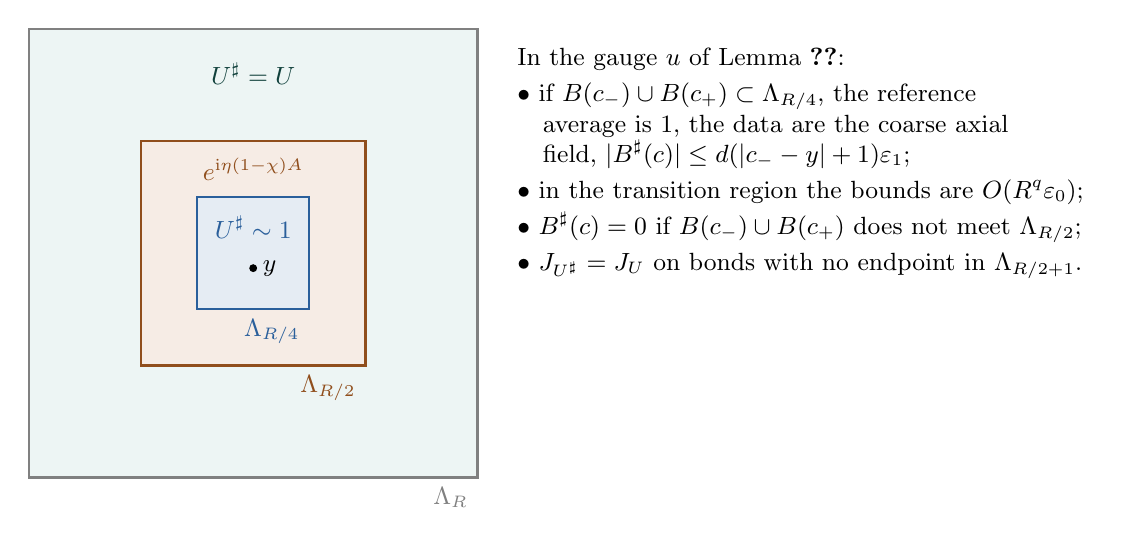
\begin{tikzpicture}[scale=0.95]
\fill[fgreen!8] (-3,-3) rectangle (3,3);
\fill[forange!12] (-1.5,-1.5) rectangle (1.5,1.5);
\fill[fblue!12] (-0.75,-0.75) rectangle (0.75,0.75);
\draw[gray,thick] (-3,-3) rectangle (3,3);
\draw[forange!80!black,thick] (-1.5,-1.5) rectangle (1.5,1.5);
\draw[fblue,thick] (-0.75,-0.75) rectangle (0.75,0.75);
\fill (0,-0.2) circle (1.5pt) node[right,font=\small] {$y$};
\node[fblue,font=\small] at (0,0.35) {$U^\sharp\sim1$};
\node[forange!80!black,font=\small] at (0,1.12) {$e^{\ii\eta(1-\chi)A}$};
\node[fgreen!50!black,font=\small] at (0,2.4) {$U^\sharp=U$};
\node[gray,font=\small,anchor=north east] at (3,-3) {$\Lam_R$};
\node[forange!80!black,font=\small,anchor=north east] at (1.5,-1.5) {$\Lam_{R/2}$};
\node[fblue,font=\small,anchor=north east] at (0.75,-0.75) {$\Lam_{R/4}$};
\node[align=left,anchor=west,font=\small] at (3.4,1.2) {In the gauge $u$ of Lemma~\ref{lem:adapted-gauge}:\\[2pt]
$\bullet$ if $B(c_-)\cup B(c_+)\subset\Lam_{R/4}$, the reference\\ \quad average is $1$, the data are the coarse axial\\ \quad field, $|B^\sharp(c)|\le d(|c_--y|+1)\eps_1$;\\[2pt]
$\bullet$ in the transition region the bounds are $O(R^q\eps_0)$;\\[2pt]
$\bullet$ $B^\sharp(c)=0$ if $B(c_-)\cup B(c_+)$ does not meet $\Lam_{R/2}$;\\[2pt]
$\bullet$ $J_{U^\sharp}=J_U$ on bonds with no endpoint in $\Lam_{R/2+1}$.};
\end{tikzpicture}
\caption{The spliced reference configuration of Definition~\ref{def:splice}.}
\label{fig:splice}
\end{figure}

\begin{lemma}[Splicing]\label{lem:splice}
There is $C_9\ge1$, depending only on $d$, $L$, $G$, $\alpha$ and $M$, with the following property. Let $R\ge16M+16$, and let $U$ be real and $(M,\eps_0)$-regular with $U\in\mathfrak U(\eps_0)$. Let $y$, $u$ and $A$ be as in Definition~\ref{def:splice}, with $\|A\|_{1,\alpha;\Lam_R(y)}\le s$ and $C_9(\eps_0+s)\le c_1$. Then:
\begin{enumerate}[label=(\alph*)]
\item $U^\sharp=U$ on all bonds with no endpoint in $\Lam_{R/2}(y)$, and $(U^\sharp)^u=1$ on the bonds of $\Lam_{R/4}(y)$.
\item $U^\sharp$ is $(M,C_9(\eps_0+s))$-regular, $|F_{U^\sharp}|\le C_9(\eps_0+s)$ and $|J_{U^\sharp}|\le\eps_0+C_9s$. Moreover $J_{U^\sharp}=J_U$ on bonds with no endpoint in $\Lam_{R/2+1}(y)$, and $J_{U^\sharp}=0$ on the bonds of $\Lam_{R/4-1}(y)$.
\item Let $W^\sharp=(U^\sharp)^{(k)}$ and $V=U^{(k)}$. For every bond $c$ of $\T$, $|\ell(V(c)W^\sharp(c)^{-1})|\le C_9(\eps_0+s)$. If $B(c_-)\cup B(c_+)$ does not meet $\Lam_{R/2}(y)$, then $W^\sharp(c)=V(c)$. If $B(c_-)\cup B(c_+)\subset\Lam_{R/4}(y)$, then $u(c_-)W^\sharp(c)u(c_+)^{-1}=1$.
\end{enumerate}
\end{lemma}

\begin{proof}
(a) follows from the definition, since $\chi=1$ on $\Lam_{R/4}(y)$.

(b) \emph{Regularity.} If $\Lam_{4M+2}(z)\subset\Lam_R(y)$, the gauge $u$ gives $(U^\sharp)^u=e^{\ii\eta(1-\chi)A}$ there, and $\|(1-\chi)A\|_{1,\alpha}\le Cs$ by the Leibniz rule, since $R\ge1$. Otherwise $|z-y|_\infty>R-4M-2$. Then every point of $\Lam_{4M+2}(z)$ has distance more than $R-8M-4\ge R/2$ from $y$, so $U^\sharp=U$ on $\Lam_{4M+2}(z)$, and the gauges of $U$ apply. The curvature is bounded in the same way, using $|F_{e^{\ii\eta B}}|\le C(|\partial B|+|B|^2)$.

\emph{Current.} The current at a bond depends only on the configuration on the plaquettes containing it and on their neighbours. This gives the two identities. In general, compute in the gauge $u$, which does not change $|J|$. For a configuration $e^{\ii\eta B}$ and a plaquette $p$ with bonds $b_1,\dots,b_4$ as in Definition~\ref{def:curvature},
\[
F^s_{e^{\ii\eta B}}(p)=\eta^{-2}\mathfrak S\big(\eta B(b_1),\eta B(b_2),\eta B(b_3),\eta B(b_4)\big),\qquad\mathfrak S(z)=P_{\mathfrak g}\sin\ell\big(e^{\ii z_1}e^{\ii z_2}e^{-\ii z_3}e^{-\ii z_4}\big),
\]
with $F^s$ as in Lemma~\ref{lem:current}. The function $\mathfrak S$ is analytic near $0$, and $\mathfrak S(z)=z_1+z_2-z_3-z_4+\mathfrak S_2(z)$ with $|\mathfrak S_2(z)|\le C|z|^2$ and $|\nabla\mathfrak S_2(z)|\le C|z|$. Let $t=1-\chi$ and $A^\sharp=tA$, and let $x_p$ be the base point of $p$. Then
\[
F^s_{e^{\ii\eta A^\sharp}}(p)=t(x_p)F^s_{e^{\ii\eta A}}(p)+E(p),
\]
\[
E(p)=\sum_{i=1}^4\pm\frac{t(b_i)-t(x_p)}\eta\,A(b_i)+\eta^{-2}\Big(\mathfrak S_2\big(\eta A^\sharp(b_1),\dots\big)-t(x_p)\,\mathfrak S_2\big(\eta A(b_1),\dots\big)\Big).
\]
Since $|\partial^\beta t|\le CR^{-|\beta|}$ and $|A|+|\partial A|\le s$, we get $|E|\le Cs$. Between neighbouring plaquettes, the arguments $\eta A^\sharp(b_i)$, $\eta A(b_i)$ and $t(x_p)$ change by at most $C\eta^2s$ and $C\eta/R$. With $|\nabla\mathfrak S_2(z)|\le C|z|$ and the product rule, the difference quotients of $E$ are bounded by $Cs$. By Lemma~\ref{lem:cov-expansion}, $D^T_{e^{\ii\eta B}}=\partial^*+T_B^T$ with $T_B$ local and bounded by $C|B|$. Using $J_{e^{\ii\eta A}}=D^T_{e^{\ii\eta A}}F^s_{e^{\ii\eta A}}=R(u)J_U$ (Lemma~\ref{lem:current}(a)),
\[
J_{e^{\ii\eta A^\sharp}}=t\,R(u)J_U+[\partial^*,t]F^s_{e^{\ii\eta A}}+\big(T^T_{A^\sharp}t-tT^T_A\big)F^s_{e^{\ii\eta A}}+D^T_{e^{\ii\eta A^\sharp}}E .
\]
Each term after the first is bounded by $Cs$, because $|F^s_{e^{\ii\eta A}}|\le Cs$ and $|\partial t|\le C/R$. Hence $|J_{U^\sharp}|\le\eps_0+Cs$.

(c) The average $U^{(k)}(c)$ depends only on the bonds of $B(c_-)\cup B(c_+)$ (Lemma~\ref{lem:one-step-basic}). This gives the first identity. The second follows from (a) and covariance, since $\mathfrak a^{(k)}(1)=1$; the gauge $u$ may be extended arbitrarily outside $\Lam_R(y)$. In the remaining case $B(c_-)\cup B(c_+)\subset\Lam_{R/2+2}(y)\subset\Lam_R(y)$. Lemma~\ref{lem:avg-local-gauge}, applied to $U^u$ and to $(U^\sharp)^u$ on the union of blocks $B(c_-)\cup B(c_+)$, gives $V^u(c)=e^{\ii B'}$ and $(W^\sharp)^u(c)=e^{\ii B''}$ with $|B'|\le s+4d\eps_0$ and $|B''|\le s+4dC'(\eps_0+s)$. Here $C'$ is the constant obtained in (b) for the curvature of $U^\sharp$. So (c) holds with $C_9\ge(1+4d)(1+C')$; the same bound applies in the second case. By covariance and Lemma~\ref{lem:log-estimates}(b), $|\ell(VW^{\sharp-1})(c)|=|\ell(e^{\ii B'}e^{-\ii B''})|\le|B'|+|B''|$.
\end{proof}

\section{Localized bounds and the local improvement}\label{sec:improvement}

\subsection{Localized bounds for the relative problem}

Theorem~\ref{thm:variational} bounds the solution in sup norms over the whole torus. Its proof gives more. By the first-order formula and the Euler--Lagrange equation, the solution near a point is controlled by the data near that point, up to exponentially decaying contributions from far away and a quadratic error.

In the setting of Theorem~\ref{thm:variational}, let $A_*$ and $\omega$ be as there. For $y\in\T$ let $c_y$ be the centre of $B(y)$, and let $u_y$ be any real gauge transformation in which $U_0$ satisfies (B) on $\Lam_4(c_y)$ with parameter $C\eps$; write $\tilde A_{*,y}=R(u_y)A_*$. The bounds below hold uniformly in the choice of $u_y$. Put
\[
\mathsf b(y)=\max\{|B(c)|:\ |c_--y|_\infty\le1\},\qquad \mathsf j(y)=\max\{|J_{U_0}(b)|:\ b_-\in B(y)\},
\]
\begin{multline*}
\mathsf N(y)=|A_*|_{\Lam_1(c_y)}+|\nabla A_*|_{\Lam_1(c_y)}+|\Lap_{U_0}A_*|_{\Lam_1(c_y)}\\
+\Hol{\partial\tilde A_{*,y}}{\Lam_1(c_y)}+\max\{|\omega(c)|:\ |c_--y|_\infty\le2\},
\end{multline*}
where $c$ runs over the bonds of $\T$.

\begin{proposition}[Localized bounds]\label{prop:localized}
There are $C_7,\gamma_7>0$, independent of $k$, $n$, $\eta$ and $U_0$, such that, under the hypotheses of Theorem~\ref{thm:variational}, for every $y\in\T$:
\begin{enumerate}[label=(\alph*)]
\item $\displaystyle\mathsf N(y)\le C_7\sum_{y'\in\T}e^{-\gamma_7|y-y'|}\big(\mathsf b(y')+\mathsf j(y')\big)+C_7(\eps+\beta)^2$;
\item the configuration $U_\flat=e^{\ii\eta A_*}U_0$, which is gauge equivalent to the minimizer $U_*$, satisfies
\[
|F_{U_\flat}(p)|\le|F_{U_0}(p)|+C_7\mathsf N(y),\qquad|J_{U_\flat}(b)|\le C_7\mathsf N(y)
\]
for all plaquettes $p$ and bonds $b$ with base point in $B(y)$.
\end{enumerate}
\end{proposition}

\begin{proof}
Throughout, sums of products of exponentially decaying kernels are again exponentially decaying, with a smaller rate; $\gamma_7$ is the rate obtained at the end. We use the pointwise bounds of Parts~II and~III at $U_0$, which hold by Corollary~\ref{cor:parts-apply}, on cubes $\Lam_1(z)$ instead of blocks (Remark~\ref{rem:cubes}).

\emph{Step 1: first derivatives.} By Theorem~\ref{thm:variational}(c), $A_*=\bH B-\bC J_{U_0}+\mathcal R$ with $|\mathcal R|_{C^1}\le C(\eps+\beta)^2$. By the pointwise bounds of Theorem~\ref{thm:reg-min} (Theorem~\ref{thm:cov-min}(b),(d)),
\[
\begin{aligned}
|\bH B|_{\Lam_1(c_y)}+|\nabla\bH B|_{\Lam_1(c_y)}&\le C\sum_{y'}e^{-\gamma|y-y'|}\mathsf b(y'),\\
|\bC J_{U_0}|_{\Lam_1(c_y)}+|\nabla\bC J_{U_0}|_{\Lam_1(c_y)}&\le C\sum_{y'}e^{-\gamma|y-y'|}\mathsf j(y').
\end{aligned}
\]
Let $\mathsf N_1(y)=|A_*|_{\Lam_1(c_y)}+|\nabla A_*|_{\Lam_1(c_y)}$. Then $\mathsf N_1(y)$ is bounded by the right-hand side of (a).

\emph{Step 2: the multiplier.} By the proof of Proposition~\ref{prop:euler-lagrange}, for every bond $c$ of $\T$ and $\beta_0\in\mathfrak g$ with $|\beta_0|=1$,
\[
\operatorname{tr}(\beta_0\,\omega(c))=\ip\varphi{J_{U_0}+\nabla\mathcal N(A_*)}+\ip{D\varphi}{DA_*},
\]
with $|\varphi(x)|+|\nabla\varphi(x)|\le Ce^{-\gamma'|x-c_-|}$. Moreover $|\nabla\mathcal N(A_*)|_\infty\le C(\eps+|A_*|_\infty)|A_*|_{C^1}\le C(\eps+\beta)^2$ by Proposition~\ref{prop:action}(a). Hence
\[
|\omega(c)|\le C\sum_{y'}e^{-\gamma'|c_--y'|}\big(\mathsf j(y')+\mathsf N_1(y')\big)+C(\eps+\beta)^2 .
\]

\emph{Step 3: second order.} By Propositions~\ref{prop:action} and~\ref{prop:euler-lagrange},
\[
D^TDA_*=d\mathcal Q(A_*)^T\omega-J_{U_0}-\nabla\mathcal N(A_*).
\]
By Proposition~\ref{prop:Q-expansion}(c), the kernel of $d\mathcal Q(A_*)^T=\bQ^T+dC_k(A_*)^T$ connects a bond $b$ only to bonds $c$ with $b_-\in S_c$. Hence $|d\mathcal Q(A_*)^T\omega|_{\Lam_1(c_y)}\le C\max\{|\omega(c)|:|c_--y|_\infty\le2\}$. Since $RD^TA_*=0$, we have $\Lap_{U_0}A_*=D^TDA_*+DP_\cV D^TA_*$. The second term is bounded on $\Lam_1(c_y)$ by $C\sum_{y'}e^{-\gamma|y-y'|}|A_*|_{B(y')}$, by the pointwise bound on $\partial P_\cV D^T$ in Proposition~\ref{prop:cov-R}(e) (Theorem~\ref{thm:reg-scalar}(g)) and $D=\partial+T$. This bounds $|\Lap_{U_0}A_*|_{\Lam_1(c_y)}$. For the H\"older quotient, write $\Lap_{U_0}$ in the gauge $u_y$ in the normal form of Lemma~\ref{lem:cov-expansion}. Then $-\Lap\tilde A_{*,y}=R(u_y)\Lap_{U_0}A_*-\sum_\mu\partial^*_\mu(a_\mu\tilde A_{*,y})-b\tilde A_{*,y}$ on $\Lam_3(c_y)$, with $|a_\mu|+[a_\mu]_\alpha+|b|\le C\eps$. Theorem~\ref{thm:local-regularity}(d) gives
\[
\Hol{\partial\tilde A_{*,y}}{\Lam_1(c_y)}\le C\Big(|\Lap_{U_0}A_*|_{\Lam_2(c_y)}+\max_{|y'-y|_\infty\le3}\mathsf N_1(y')\Big).
\]
The cube $\Lam_2(c_y)$ is covered by the cubes $\Lam_1(c_{y'})$ with $|y'-y|_\infty\le1$; the values of $\omega$ that enter there are bounded by Step~2 for all bonds. Combining Steps 1--3 gives (a).

(b) By \eqref{eq:plaquette-product}, $U_\flat(\partial p)=e^{\ii\eta^2\zeta_p(A_*)}U_0(\partial p)$ with $|\zeta_p(A_*)|\le C(|A_*|+|\nabla A_*|)$ on the bonds of $p$. Lemma~\ref{lem:log-estimates}(b) gives the bound on the curvature. By Proposition~\ref{prop:action}(d) and Proposition~\ref{prop:euler-lagrange}, $J_{U_\flat}=\Psi(A_*)^{-T}d\mathcal Q(A_*)^T\omega$. As in Step 3, this is bounded at $b$ by $C\max\{|\omega(c)|:|c_--y|_\infty\le2\}$.
\end{proof}

\subsection{The local improvement}

\begin{lemma}[Local improvement]\label{lem:improvement}
There are $\eps_{\rm imp}>0$, $C_{\rm imp}\ge1$ and an integer $n_0$, depending only on $d$, $L$, $G$, $a$, $\alpha$ and $M$, with the following property. Let $k\ge1$, $n\ge n_0$, and let $V\in\mathfrak U_k(\eps_1)$ be a real configuration on $\T$. Let $U\in\mathfrak B(V)$ be a critical point of $S|_{\mathfrak B(V)}$. Suppose that $U$ is $(M,\eps_0)$-regular and $U\in\mathfrak U(\eps_0)$, with $\eps_0\le\eps_{\rm imp}$. Then $U$ is $(M,\eps_0')$-regular and $U\in\mathfrak U(\eps_0')$, where
\[
\eps_0'=C_{\rm imp}\eps_1+\tfrac12\eps_0 .
\]
If $\eps_0'>1$, the regularity conclusion is read as $(M,1)$-regularity; it gives the three bounds of Definition~\ref{def:regular} with $\eps_0'$ in place of $\eps$.
\end{lemma}

The point is that $C_{\rm imp}$ does not depend on $\eps_0$. Iterating the lemma brings the regularity parameter down to $2C_{\rm imp}\eps_1$, whatever the a priori bound, as long as the latter is at most $\eps_{\rm imp}$.

\begin{proof}
If $\eps_1>2\eps_0$ there is nothing to prove, since then $\eps'_0\ge\eps_0$. So let $\eps_1\le2\eps_0$.

\emph{Choice of constants.} Let $C_7,\gamma_7$ be as in Proposition~\ref{prop:localized}, $C_8,q$ as in Lemma~\ref{lem:adapted-gauge}, and $C_9$ as in Lemma~\ref{lem:splice}. Put
\[
K_R=2C_9\big(1+C_8R^q\big),\qquad S_1=\sum_{w\in\Z^d}e^{-\gamma_7|w|}(1+|w|),\qquad T(t)=\sum_{w\in\Z^d,\,|w|_\infty>t}e^{-\gamma_7|w|},
\]
and $K_1=\max(5,C_7)$. Fix an integer $R\ge64(M+1)$ with
\[
K_1C_7K_R\,T(R/8)\le\tfrac14 ;
\]
this is possible because $K_R$ grows polynomially and $T$ decays exponentially. Let $n_0=4R+16$. Choose $\eps_{\rm imp}$ so small that $K_1C_7K_R^2\eps_{\rm imp}\le\frac14$, $K_R\eps_{\rm imp}\le c_6$, $\eps_{\rm imp}\le\theta_0$, $C_8R^q\eps_{\rm imp}\le1$ and $C_9(1+C_8R^q)\eps_{\rm imp}\le c_1$.

\emph{Step 1: the adapted gauge.} Fix $y\in\T$. By Lemma~\ref{lem:adapted-gauge} there is a real gauge transformation $u$ on $\Lam_R(y)$ with $U^u=e^{\ii\eta A}$, $\|A\|_{1,\alpha;\Lam_R(y)}\le s:=C_8R^q\eps_0$, and $V^u(c)=e^{\ii B_y(c)}$ with $|B_y(c)|\le d(|c_--y|_\infty+1)\eps_1$ for the bonds of $\T$ in $\Lam_R(y)$.

\emph{Step 2: the spliced reference.} Let $U^\sharp$ be the spliced configuration of Definition~\ref{def:splice}, built with this $u$. By Lemma~\ref{lem:splice}, $U^\sharp$ is $(M,\eps^\sharp)$-regular with $|J_{U^\sharp}|\le\eps^\sharp$, where $\eps^\sharp=C_9(\eps_0+s)$. Moreover $V(c)W^\sharp(c)^{-1}=e^{\ii B^\sharp(c)}$ with $|B^\sharp|_\infty\le\beta^\sharp:=C_9(\eps_0+s)$, where $W^\sharp=(U^\sharp)^{(k)}$. Then $\eps^\sharp+\beta^\sharp\le K_R\eps_0\le c_6$. So Theorem~\ref{thm:variational} applies with the reference $U^\sharp$ and the coarse configuration $V$.

\emph{Step 3: identification.} By Theorem~\ref{thm:variational}(a), $S|_{\mathfrak B(V)}$ has exactly one critical orbit in $\mathfrak B(V)\cap\mathfrak U(\theta_0)$. Since $U$ is critical and lies in $\mathfrak U(\eps_0)\subset\mathfrak U(\theta_0)$, it belongs to this orbit. Hence $U=(e^{\ii\eta A^\sharp_*}U^\sharp)^v$ for a real gauge transformation $v$, where $A^\sharp_*$ is the Landau representative relative to $U^\sharp$. Applying $u$, we get on the bonds of $\Lam_{R/4}(y)$, where $(U^\sharp)^u=1$,
\[
U^{uv^{-1}}=e^{\ii\eta\tilde A},\qquad\tilde A=R(u)A^\sharp_* .
\]
In this gauge $\nabla_{U^\sharp}$ is the ordinary difference, and $u$ is a gauge in which $U^\sharp$ satisfies (B) near every block in $\Lam_{R/4-4}(y)$.

\emph{Step 4: the data near $y$.} Apply Proposition~\ref{prop:localized} with reference $U^\sharp$. Let $y'\in\T$ with $|y'-y|_\infty\le R/4-3$. Every bond $c$ with $|c_--y'|_\infty\le1$ has $B(c_-)\cup B(c_+)\subset\Lam_{R/4}(y)$. So, by Lemma~\ref{lem:splice}(c), $(W^\sharp)^u(c)=1$, and
\[
|B^\sharp(c)|=|\ell(V^u(c))|=|B_y(c)|\le d(|y'-y|_\infty+2)\eps_1 .
\]
Moreover $\mathsf j(y')=0$ by Lemma~\ref{lem:splice}(b). For the remaining $y'$ we only use $\mathsf b(y')+\mathsf j(y')\le K_R\eps_0$. Let $y_1\in\T$ with $|y_1-y|_\infty\le4M+4$. For $|y'-y|_\infty>R/4-3$ we have $|y_1-y'|_\infty>R/8$, because $R\ge64(M+1)$. Therefore
\[
\mathsf N(y_1)\le C_7dS_1(4M+7)\,\eps_1+C_7K_R\,T(R/8)\,\eps_0+C_7K_R^2\eps_0^2 .
\]

\emph{Step 5: conclusion.} Let $z\in\Tf$, and choose $y\in\T$ with $|z-y|_\infty\le1$. Then $\Lam_{4M+2}(z)\subset\Lam_{4M+3}(y)\subset\Lam_{R/4-4}(y)$. By Step 3, $U^{uv^{-1}}=e^{\ii\eta\tilde A}$ on $\Lam_{4M+2}(z)$. On it, $|\tilde A|$, $|\partial\tilde A|$ and the H\"older quotients of $\partial\tilde A$ on cubes $\Lam_1(c_{y_1})$ are bounded by $\mathsf N(y_1)$, with the gauge $u_{y_1}=u$. Put $H=\max_{|y_1-y|_\infty\le4M+4}\mathsf N(y_1)$. Let $x\ne x'$ be points of a cube $\Lam_3(z')\subset\Lam_{4M+2}(z)$. If $|x-x'|_\infty<\frac12$, then in each coordinate $x$ and $x'$ differ by a multiple of $\eta=1/N$ less than $\frac12$, hence by at most $\frac12-\frac\eta2$, and by at most $\frac12-\eta$ if $N$ is even. A difference involves points at most $2\eta$ beyond its base point in each coordinate (for $\partial_\mu\tilde A_\mu$, the point $x+2\eta e_\mu$). So the points of the two differences span, in each coordinate, an interval of length at most $\frac12+\frac{3\eta}2\le1$ if $N\ge3$ is odd, and at most $\frac12+\eta\le1$ if $N$ is even. The centres $c$ with $|p-c|_\infty\le1$ for all these points $p$ form, in each coordinate, a closed interval of length at least $1$. The block centres form a grid of spacing $1$, so one of them lies in it: these points lie in a common cube $\Lam_1(c_{y_1})$, and then $|y_1-y|_\infty\le4M+4$. If $|x-x'|_\infty\ge\frac12$, the H\"older quotient is at most $4\sup|\partial\tilde A|$. Hence $|\tilde A|\le H$, $|\partial\tilde A|\le H$, and the H\"older quotients of $\partial\tilde A$ on the cubes $\Lam_3(z')\subset\Lam_{4M+2}(z)$ are at most $4H$. These are the three bounds of Definition~\ref{def:regular}, and each is at most $K_1H$, since $K_1\ge5$. By Proposition~\ref{prop:localized}(b), with $F_{U^\sharp}=0$ near $y$, the curvature and the current of $U$ on the plaquettes and bonds based in $B(y)$ are bounded by $C_7\mathsf N(y)$. All these quantities are gauge invariant. Every plaquette and bond is based in some block, and every $z$ is close to some $y$. With the choice of $R$ and $\eps_{\rm imp}$, Step~4 gives the lemma with $C_{\rm imp}=K_1C_7dS_1(4M+7)$:
\[
K_1\max\mathsf N\le C_{\rm imp}\eps_1+\tfrac14\eps_0+\tfrac14\eps_0 .\qedhere
\]
\end{proof}

\begin{remark}[Comparison with {\cite[Sect.~F]{BalVar}}]
The structure of the argument is Ba\l aban's: near a point the minimizer equals, up to small errors, $\bH$ applied to the coarse field in an axial gauge centred at the point; the latter grows only linearly with the distance, with slope given by the curvature of $V$, while $\bH$ decays exponentially. Compare \cite[(159)--(167)]{BalVar}. The difference is in how the problem is localized. Ba\l aban formulates a new variational problem on a nested sequence of cubes around the point. The configuration is frozen outside, and the problem is solved relative to the trivial configuration. Here the problem is not changed. Only the reference configuration is changed, and Theorem~\ref{thm:variational} is applied once more on the torus. This is possible because that theorem is uniform in the reference. The splicing is a purely geometric operation (Lemma~\ref{lem:splice}). As in \cite[(166)]{BalVar}, the quadratic error forces the a priori bound to be small in terms of the localization radius.
\end{remark}

\section{The induction over the number of steps}\label{sec:induction}

We now prove Ba\l aban's variational theorem on the torus by induction over $k$. Each step has three parts:
\begin{itemize}
\item the solution of the $(k-1)$-step problem for the trivial extension of $V$ is a reference with \emph{exactly} the right averages \cite[Sect.~A]{BalVar};
\item Theorem~\ref{thm:variational} solves the problem near this reference, with an a priori regularity bound that is worse by a power of $L$;
\item Lemma~\ref{lem:improvement}, iterated, restores the regularity bound with a constant independent of $k$.
\end{itemize}

\subsection{The trivial extension}

Let $k\ge1$. A bond $b$ of $\T^{(k-1)}$ in direction $\mu$ is a \emph{crossing bond} if its endpoints lie in different blocks, $b_-\in B_k(y)$ and $b_+\in B_k(y+e_\mu)$; we then write $c(b)=(y,y+e_\mu)$. For a configuration $V$ on $\T$ define $V_0$ on $\T^{(k-1)}$ by
\[
V_0(b)=V(c(b))\ \text{ for crossing bonds},\qquad V_0(b)=1\ \text{ for bonds inside a block}
\]
\cite[(11)]{BalVar}.

\begin{lemma}[Trivial extension]\label{lem:trivial-extension}
\begin{enumerate}[label=(\alph*)]
\item $\mathfrak a_k(V_0)=V$.
\item Let $p$ be a plaquette of $\T^{(k-1)}$. If $p$ has crossing bonds in both of its directions, then $V_0(\partial p)=V(\partial p')$, where $p'$ is the plaquette of $\T$ spanned by the four blocks containing the corners of $p$. Otherwise $V_0(\partial p)=1$. Hence $F_{V_0}(p)=L^2F_V(p')$ or $0$, and $V\in\mathfrak U_k(\eps_1)$ implies $V_0\in\mathfrak U_{k-1}(L^2\eps_1)$.
\end{enumerate}
\end{lemma}

\begin{proof}
(a) Let $c=(y,y+e_\mu)$ and $x\in B_k(y)$. The pieces $\Gamma^k_{y,x}$ and $\Gamma^k_{y+e_\mu,x(c)}$ of $\Gamma^k_{c,x}$ stay inside blocks. The straight piece $[x,x(c)]$ contains exactly one crossing bond, from $B_k(y)$ to $B_k(y+e_\mu)$. The same holds for $[c]$. Hence $V_0(\Gamma^k_{c,x})=V(c)=V_0([c])$, all logarithms in Definition~\ref{def:one-step} vanish, and $\mathfrak a_k(V_0)(c)=V_0([c])=V(c)$.

(b) The two bonds of $p$ in direction $\mu$ are crossing or not simultaneously, and they connect the same pair of blocks if the bonds in direction $\nu$ do not cross. In that case $V_0(\partial p)$ is $V(c)V(c)^{-1}=1$ or $1$. If both pairs cross, the four bonds carry the values of $V$ on the four bonds of $\partial p'$, in the order of Definition~\ref{def:curvature}. Finally $F_{V_0}(p)=\delta_{k-1}^{-2}\ell(V_0(\partial p))=L^2\ell(V(\partial p'))=L^2F_V(p')$.
\end{proof}

In units of $\delta_{k-1}$, curvatures are multiplied by $\delta_{k-1}^2=L^{-2}$. So in its own units, $V_0$ satisfies the same curvature bound $\eps_1$ as $V$.

\subsection{Change of units}

As in the proof of Theorem~\ref{thm:chart}, the $(k-1)$-step structure on $(\Tf,\T^{(k-1)})$, in units of $\delta_{k-1}$, is the $(k-1)$-step structure on a torus of side $Ln$ with fine spacing $L\eta$. The Wilson action changes by a constant factor, so critical points and minimizers are the same.

\begin{lemma}[Change of units]\label{lem:units}
There is $C_L$, depending only on $d$, $\alpha$, $G$, $L$ and $M$, with the following property. Let $U_0$ be a real configuration on $\Tf$ which, in units of $\delta_{k-1}$, lies in $\mathfrak U(\theta)$ and is $(M,\theta)$-regular. If $C_L\theta\le1$, then in units of $\delta_k=1$, $U_0\in\mathfrak U(L^3\theta)$ and $U_0$ is $(M,C_L\theta)$-regular.
\end{lemma}

\begin{proof}
Passing to units of $\delta_k$ divides lengths by $L$ and multiplies Lie fields by $L$, their differences and curvatures by $L^2$, currents by $L^3$, and H\"older quotients of differences by $L^{2+\alpha}$. This gives the first claim. For the second, let $r'=(4M+2)/L$. Every cube $\Lam_{r'}(z)$ carries a gauge with $|A|\le L\theta$ and $|\partial A|\le L^2\theta$, and with H\"older quotients of $\partial A$ at most $L^{2+\alpha}\theta$ on cubes of radius $3/L$. Let $r=r'-2$. Two points of $\Lam_r(z)$ at distance at most $3/L$ lie in a common cube of radius $3/L$ contained in $\Lam_{r'}(z)$. For points at larger distance the quotient is at most $2|\partial A|(L/3)^\alpha$. Hence $U_0$ is $3L^3\theta$-regular on every cube $\Lam_r(z)$. Since $M\ge5L$, $r\ge18$. Lemma~\ref{lem:large-cubes} with $R=4M+2$ gives the claim, with $C_L=3C_E(4M+2)^{p+1}L^3$.
\end{proof}

\subsection{The theorem}

\begin{theorem}[Ba\l aban's variational theorem on the torus]\label{thm:balaban}
Assume the conventions of Part~VI, in particular $M\ge\max(M_0,5L)$. Let $d\ge3$, and let $\theta_0$ be as in Theorem~\ref{thm:variational} and $n_0$ as in Lemma~\ref{lem:improvement}. There are $a_1,B_3>0$, depending only on $d$, $L$, $G$, $a$, $\alpha$ and $M$, such that the following holds for all $k\ge0$, all $n\ge n_0$ and every real configuration $V$ on $\T$ with $V\in\mathfrak U_k(\eps_1)$, $\eps_1\le a_1$.
\begin{enumerate}[label=(\alph*)]
\item $S|_{\mathfrak B(V)}$ has exactly one critical orbit in $\mathfrak B(V)\cap\mathfrak U(\theta_0)$. This orbit is the set of minimizers of $S$ on $\mathfrak B(V)\cap\mathfrak U(\theta_0)$.
\item Every element $U_k(V)$ of this orbit lies in $\mathfrak U(B_3\eps_1)$ and is $(M,B_3\eps_1)$-regular.
\end{enumerate}
The constants do not depend on $k$, $n$ or $\eta$.
\end{theorem}

This is \cite[Theorem~1]{BalVar} for a single torus with the small-field condition everywhere. Part~(b) is the regularity statement \cite[(8)--(10)]{BalVar} for cubes of the fixed size $M$. As in \cite{BalVar}, the elements of the orbit are called \emph{background fields} or \emph{minimal configurations}.

\begin{proof}
\emph{Constants.} Let $C_{\rm base}$ be the constant of the case $k=0$ below, and put
\[
B_3=\max(4C_{\rm imp},C_{\rm base}),\qquad K=(1+C_6)C_L .
\]
Choose $a_1$ so small that $C_LB_3a_1\le\min(c_6,1)$, $KB_3a_1\le\eps_{\rm imp}$, $B_3a_1\le\theta_0$, and $a_1\le c_1$, $d(8M+6)a_1\le c_G$. These choices do not depend on $k$.

\emph{The case $k=0$.} Then $\eta=1$, $\Tf=\T$, $\mathfrak B(V)=\{V\}$ and $\mathfrak G_0=\{1\}$. We first prove (b); then $V\in\mathfrak U(B_3\eps_1)\subset\mathfrak U(\theta_0)$, and (a) is trivial. The current $J_V=D^T_VF^s_V$ is a combination of at most $4d$ values of $F^s_V$, so $|J_V|\le C\eps_1$. For regularity, fix $z$ and a point $z_0\in\T$ with $|z-z_0|_\infty\le1$, and let $u$ be the axial gauge on $\Lam_{4M+2}(z)$ with $V^u(\Gamma^{\rm ax}_{z_0,x})=1$. As in the proof of Lemma~\ref{lem:adapted-gauge}, $|\ell(V^u(b))|\le d(4M+4)\eps_1$ for every bond $b$ of $\Lam_{4M+2}(z)$. On the unit lattice, for $A=\ell(V^u)$, $|\partial A|\le2|A|$, and the H\"older quotients of $\partial A$ are at most $2|\partial A|\le4|A|$, since distinct points have distance at least $1$. So $V$ is $(M,C_{\rm base}\eps_1)$-regular and lies in $\mathfrak U(C_{\rm base}\eps_1)$, with $C_{\rm base}$ depending only on $d$, $G$ and $M$.

\emph{From $k-1$ to $k$.} Let $V\in\mathfrak U_k(\eps_1)$ with $\eps_1\le a_1$, and let $V_0$ be its trivial extension. In units of $\delta_{k-1}$ the torus has side $Ln\ge n_0$, and $V_0$ has curvature at most $\eps_1$ (Lemma~\ref{lem:trivial-extension}). By the induction hypothesis there is a minimal configuration $U_0=U_{k-1}(V_0)$. In units of $\delta_{k-1}$ it lies in $\mathfrak U(B_3\eps_1)$ and is $(M,B_3\eps_1)$-regular. By Lemma~\ref{lem:units}, in units of $\delta_k$,
\[
U_0\in\mathfrak U(L^3B_3\eps_1),\qquad U_0\ \text{is}\ (M,\eps)\text{-regular},\qquad\eps:=C_LB_3\eps_1\le c_6 .
\]
Since $U_0^{(k-1)}=V_0$, Lemma~\ref{lem:trivial-extension}(a) gives
\[
W_k=U_0^{(k)}=\mathfrak a_k(V_0)=V ,
\]
so the hypotheses of Theorem~\ref{thm:variational} hold with $\beta=0$; note $|J_{U_0}|\le L^3B_3\eps_1\le\eps$. Parts (a) and (b) of that theorem give (a).

For (b), let $U$ be an element of the orbit. By Theorem~\ref{thm:variational}(e), $U$ is $(M,\eps_0^{(0)})$-regular and lies in $\mathfrak U(\eps_0^{(0)})$, with $\eps_0^{(0)}=(1+C_6)\eps=KB_3\eps_1\le\eps_{\rm imp}$. If $\eps_0^{(0)}\le B_3\eps_1$ there is nothing to prove, so let $\eps_0^{(0)}>B_3\eps_1\ge4C_{\rm imp}\eps_1$. Define $\eps_0^{(m+1)}=C_{\rm imp}\eps_1+\frac12\eps_0^{(m)}$. If $\eps_0^{(m)}\ge2C_{\rm imp}\eps_1$, then $\eps_0^{(m+1)}\le\eps_0^{(m)}$. By Lemma~\ref{lem:improvement} and induction over $m$, $U$ is $(M,\eps_0^{(m)})$-regular and lies in $\mathfrak U(\eps_0^{(m)})$ for all $m$. Since
\[
\eps_0^{(m)}-2C_{\rm imp}\eps_1=2^{-m}\big(\eps_0^{(0)}-2C_{\rm imp}\eps_1\big)\le2^{-m}KB_3\eps_1 ,
\]
we have $\eps_0^{(m)}\le2C_{\rm imp}\eps_1+\frac12B_3\eps_1\le B_3\eps_1$ once $2^{m}\ge2K$. This proves (b) with the same $B_3$, and closes the induction.
\end{proof}

The induction uses Theorem~\ref{thm:variational} with $\beta=0$: the reference has exactly the prescribed averages. On the nested domains of \cite{BalVar} this is not the case, and $\beta$ is of order $\eps_1$ \cite[(14)]{BalVar}. Theorem~\ref{thm:variational} allows $\beta>0$, which is used in Lemma~\ref{lem:improvement} and in Corollary~\ref{cor:analytic} below.

\subsection{Consequences}

\begin{corollary}[Local regularity from gauge-invariant conditions]\label{cor:regularity}
There are $a_2,B_5>0$, depending only on $d$, $L$, $G$, $a$, $\alpha$ and $M$, such that for all $k\ge0$ and $n\ge n_0$ every real configuration $U\in\mathfrak U(\theta)$ on $\Tf$ with $\theta\le a_2$ is $(M,B_5\theta)$-regular. More precisely, $U$ is gauge equivalent, by a real gauge transformation, to $e^{\ii\eta A}U_k(U^{(k)})$. Here $A$ lies in Ba\l aban's Landau gauge relative to $U_k(U^{(k)})$, and $A$ obeys the bounds of Theorem~\ref{thm:chart} with $\eps+\theta+\beta=(2B_3+1)\theta$.
\end{corollary}

\begin{proof}
Let $k=0$. Then $\eta=1$, $\Tf=\T$ and $U^{(0)}=U$. By the case $k=0$ of the proof of Theorem~\ref{thm:balaban}, $\mathfrak B(U)=\{U\}$, so $U_0(U)=U$, and the representation holds with $A=0$, for which the gauge condition and the bounds are trivial. The curvature of $U$ is at most $\theta\le a_1$, so Theorem~\ref{thm:balaban}(b), with $V=U$ and $\eps_1=\theta$, shows that $U$ is $(M,B_3\theta)$-regular.

Let $k\ge1$ and $V=U^{(k)}$. By Proposition~\ref{prop:avg-regular}, $V\in\mathfrak U_k(2\theta)$. Let $2\theta\le a_1$ and $(2B_3+1)\theta\le c_4$. By Theorem~\ref{thm:balaban}, $U_0=U_k(V)$ exists. It is $(M,2B_3\theta)$-regular, satisfies $|J_{U_0}|\le2B_3\theta$, and has $U_0^{(k)}=V$. By Lemma~\ref{lem:axial}(c), the $\mathfrak G_0$-orbit of $U$ contains a configuration $U^{\rm ax}$ with $U'=U^{\rm ax}U_0^{-1}\in\mathrm{Ax}_k$. Transformations in $\mathfrak G_0$ do not change the averages, so $U'^{[k]}=(U^{\rm ax})^{(k)}V^{-1}=1$. Theorem~\ref{thm:chart}, with $\eps=2B_3\theta$ and $\beta=0$, gives $\tilde U=e^{\ii\eta A}$ in the Landau gauge with $(\tilde UU_0)^{\mathsf w_k(\tilde U)}=U^{\rm ax}$ and with the stated bounds. Finally, $e^{\ii\eta A}U_0$ is $(M,2B_3\theta+CB_1(2B_3+1)\theta)$-regular, by the argument in the proof of Proposition~\ref{prop:minimizer-regularity}(c). That argument uses the H\"older bound on the unit cubes $\Lam_1(z)$. For the field $A$ of Theorem~\ref{thm:chart} this bound is given by the proof of Proposition~\ref{prop:a-priori} (Theorem~\ref{thm:local-regularity}(d)) and Remark~\ref{rem:cubes}. So the corollary holds with $B_5=2B_3+CB_1(2B_3+1)$, which is at least the constant $B_3$ of the case $k=0$.
\end{proof}

Corollary~\ref{cor:regularity} is the torus version of \cite[Sect.~F, Prop.~6]{BalReg} and of the regularity conditions \cite[(3.35)--(3.36)]{BalBackground}. It removes the hypothesis of Part~III for all configurations of Ba\l aban's small-field class: on tori of side $n\ge n_0$, regularity follows from the gauge-invariant bounds on curvature and current. The proof uses the background field as a reference: the local gauges are the Landau gauge relative to $U_k(U^{(k)})$, composed with the local gauges of the background field. The latter come out of the induction.

\begin{corollary}[Analyticity around a background field {\cite[Sect.~G]{BalVar}}]\label{cor:analytic}
Let $V$ be as in Theorem~\ref{thm:balaban}, and let $U_0$ be an element of its minimal orbit. For $k\ge1$, Theorem~\ref{thm:variational} applies with this reference and $\eps=B_3\eps_1$. For real $B$ on $\T$ with $|B|_\infty\le\beta$ and $B_3\eps_1+\beta\le c_6$, the critical orbit for $e^{\ii B}V$ in $\mathfrak B(e^{\ii B}V)\cap\mathfrak U(\theta_0)$ is unique, and its Landau representative $A_*(B)$ relative to $U_0$ satisfies $A_*(0)=0$. The map $B\mapsto A_*(B)$ extends analytically to complex $B$, and $dA_*(B)\delta B$ decays exponentially away from the support of $\delta B$, as in Theorem~\ref{thm:variational}(f).
\end{corollary}

\begin{proof}
$U_0$ is $(M,B_3\eps_1)$-regular with $|J_{U_0}|\le B_3\eps_1$, and $W_k=V$. For $B=0$, the configuration $U_0=\mathsf U(0)$ is critical, and $A=0$ lies in the Landau gauge with $\mathcal Q(1)=1$; by uniqueness, $A_*(0)=0$. For $k\ge1$ the rest is Theorem~\ref{thm:variational}.

Let $k=0$. The operators of Parts~II--V need $k\ge1$ (Section~\ref{sec:setup}), but the conclusions hold directly. Here $\eta=1$, $\Tf=\T$, $\mathfrak G_0=\{1\}$ and $U_0=V$, by the case $k=0$ of the proof of Theorem~\ref{thm:balaban}. The averaging, the correspondence transformation and $\mathcal Q$ are the identity, so $\mathfrak B(e^{\ii B}V)=\{e^{\ii B}V\}$, and the relative field of $e^{\ii B}V$ is $A_*(B)=B$; the Landau gauge condition is void. By Lemma~\ref{lem:log-estimates}(b), the curvature of $e^{\ii B}V$ is at most $\eps_1+4|B|_\infty$, and its current, a combination of at most $4d$ values of $F^s$, is at most $4d$ times this. Since $\eps_1\le B_3\eps_1$, both are at most $20d\,c_6\le\min(\theta_0,c_1)$, by the choice of $c_6$ in the proof of Theorem~\ref{thm:variational}. So the configuration $e^{\ii B}V$ lies in $\mathfrak U(\theta_0)\cap\mathfrak U_0(c_1)$, and its orbit is the unique critical orbit. The map $B\mapsto B$ is entire, $A_*(0)=0$, and $|A_*(B)|_{C^1}\le3|B|_\infty$ by \eqref{eq:lattice-trick}. Finally $dA_*(B)\delta B=\delta B$ is supported on the bond $c$, and its covariant gradient on the bonds within distance $1$ of $c$. This is the decay of Theorem~\ref{thm:variational}(f), with $C_6\ge3e^{\gamma'}$.
\end{proof}

\begin{remark}[Cubes of size of order $\eps_1^{-1}$]\label{rem:large-cubes}
Ba\l aban also proves gauges on cubes of side $2M'\le c\,\eps_1^{-1}$, with bounds $B_3M'\eps_1$ linear in the size \cite[(9), (10)]{BalVar}. Theorem~\ref{thm:balaban} and Lemma~\ref{lem:large-cubes} give gauges on cubes of side $2R$ with bounds $C(R/M)^pB_3\eps_1$, polynomial in $R$, for $R^{p+1}\eps_1$ small. Linear bounds should follow by running Lemma~\ref{lem:improvement} with a splicing radius proportional to $R$, with $R$ limited to a power of $\eps_1^{-1}$ by the quadratic error. We do not prove this. The regularity at the fixed scale $M$ is all that Parts~II--V require.
\end{remark}


\part*{Part VII: One step of the renormalization group}
\addcontentsline{toc}{part}{Part VII: One step of the renormalization group}
\section{The renormalization group transformation}\label{sec:rg-step}

This part carries out one step of Ba\l aban's renormalization group for pure Yang--Mills theory in the small-field region \cite{BalUV3}. The plan and the target are described in the companion blueprint (\texttt{RG-blueprint}) \cite{Blueprint}, referred to below as ``the blueprint''. Here we derive an exact representation of one step as a Gaussian integral around the background field, and we prove the linear estimates on which the analysis of that integral rests:
\begin{itemize}
\item the coercivity and decay of the fluctuation covariance;
\item the analyticity of the coarse effective action and the decay of its derivatives;
\item the structure of the background-dependent normalization.
\end{itemize}
The polymer expansion of the interaction, its renormalization and the iteration are the subject of later parts.

\paragraph{Conventions for Part VII.} We keep the conventions of Parts~IV--VI. In addition $d=3$ in the statements about couplings, although the constructions of this part work for $d\ge3$, and $G$ is semisimple. Semisimplicity is not used in this part; it is needed for the renormalization in the next one. We work in the \emph{units of step $k$}: the unit lattice is $\T=\T^{(k)}$, the fine lattice is $\Tf$ with $\eta=L^{-k}$, and the next coarse lattice is $\T'=\T^{(k+1)}$, of spacing $L$. Its blocks are $B'(y)=B_{k+1}(y)$, with $L^d$ points of $\T$, and the one-step averaging is $\mathfrak a'=\mathfrak a_{k+1}$. The torus $\T$ has side $Ln$, where $n$ is the side of $\T'$ in its own units. We assume $n\ge n_{\delta=1}$, with $n_\delta$ from Proposition~\ref{prop:sharp-curvature}, and $n\ge80M'_L$, with $M'_L$ from Theorem~\ref{thm:step-coercive}. Fields on $\T$ carry the unweighted norm $\|Z\|^2=\sum_b|Z(b)|^2$.

\subsection{The model and the transformation}

Let $\epsilon=L^{-N}$ be the finest lattice spacing, $g$ the bare coupling, and $g_k^2=g^2L^k\epsilon$ the dimensionless coupling at step $k$. The initial density on the $\epsilon$-lattice is $\rho_0(U)=\exp(-g_0^{-2}S_{\rm lat}(U)-E_0)$, where $S_{\rm lat}(U)=\sum_p(\mathsf N-\operatorname{Re}\operatorname{tr}U(\partial p))$. In the units of step $k$ the $\epsilon$-lattice has spacing $\eta=L^{-k}$, and $g_0^{-2}S_{\rm lat}=g_k^{-2}S$ with the action $S$ of Section~\ref{sec:action}. Indeed $S=\eta^{d-4}S_{\rm lat}$, $d=3$, and $g_0^2=g_k^2\eta$.

The averaging $\mathfrak a'$ uses logarithms, so it is defined only on part of the configuration space. Let $\operatorname{dom}\mathfrak a'$ be the set of real configurations $V$ on $\T$ such that, for every positively oriented bond $c$ of $\T'$ and every $x\in B'(c_-)$,
\[
\big|V(\Gamma^{k+1}_{c,x})\,V([c])^{-1}-1\big|\le c_G .
\]
For $V\in\operatorname{dom}\mathfrak a'$ the logarithms in Definition~\ref{def:one-step} are defined and lie in $\mathfrak g$, by the choice of $c_G$ (Section~\ref{sec:averaging}), so $\mathfrak a'(V)$ is defined and real. Outside this set a logarithm may be undefined or may leave $\mathfrak g$. The set $\operatorname{dom}\mathfrak a'$ is closed, and $\mathfrak a'$ is continuous on it. It is invariant under real gauge transformations $u$, which conjugate the holonomies above by $u(c_-)$. It contains $\mathfrak U_k(b)$ whenever $dbL^2\le c_G$: by Lemma~\ref{lem:one-step-basic}(a), with $\delta_{k+1}=L$, the logarithms of these holonomies are bounded by $dbL^2$, and $|h-1|\le|\ell(h)|$ for $h\in G$. If $dbL^2<c_G$, it contains $\mathfrak U_k(b)$ in its interior.

For an integrable density $\rho$ on configurations $V$ on $\T$ that vanishes outside $\operatorname{dom}\mathfrak a'$, let $T\rho$ be the image of the measure $\rho(V)\prod_bdV(b)$ under $\mathfrak a'$:
\[
\int\varphi\,d(T\rho)=\int\prod_bdV(b)\ \varphi\big(\mathfrak a'(V)\big)\,\rho(V)
\]
for bounded Borel functions $\varphi$ of configurations on $\T'$. Here $b$ runs over the positively oriented bonds of $\T$, and $dV(b)$ is the normalized Haar measure. With $\varphi=1$, the total mass of $T\rho$ is $\int\prod_bdV(b)\,\rho(V)$. We write
\begin{equation}\label{eq:rg-map}
(T\rho)(V')=\int\prod_{b}dV(b)\ \prod_{c}\delta\big(\mathfrak a'(V)(c)\,V'(c)^{-1}\big)\ \rho(V),
\end{equation}
where $c$ runs over the positively oriented bonds of $\T'$ and $\delta$ is the $\delta$-function of $G$ at $1$ with respect to the Haar measure. This formula is a notation for the image measure. If $\delta$ is replaced by a continuous function $\delta_n\ge0$ on $G$ with $\int\delta_n=1$, supported in a neighbourhood of $1$ that shrinks as $n\to\infty$, the right side is a continuous density, and the measures with these densities converge weakly to $T\rho$: for continuous $\varphi$ this follows from Fubini's theorem, the invariance of the Haar measure and the uniform continuity of $\varphi$. The left side denotes a density of $T\rho$ with respect to $\prod_cdV'(c)$, and it is used only where such a density exists. A sufficient condition is that $\rho$ vanishes outside an open subset of $\operatorname{dom}\mathfrak a'$ on which $\mathfrak a'$ is a submersion, i.e.\ its derivative has rank $\dim\mathfrak g$ times the number of positively oriented bonds of $\T'$. Then, near each point of this set, $\mathfrak a'$ is a coordinate projection in suitable analytic coordinates, and for almost every $V'$ the density at $V'$ is the integral of $\rho$ over the fibre $\{\mathfrak a'(V)=V'\}$ with respect to the measure that the two Haar measures induce on it. Integrability of $\rho$ alone does not make this fibre integral finite at every $V'$. If $\rho$ is a bounded Borel function and vanishes outside a compact subset of the open set, the fibre integral converges absolutely at every $V'$; it is then taken as the density at every $V'$, and the usual rules for $\delta$-functions compute it. In that case $\int\prod_cdV'(c)\,(T\rho)(V')=\int\prod_bdV(b)\,\rho(V)$. The density is used only for the small-field step below. There the integrand is bounded, and the cutoff confines it to a compact subset of the region of Lemma~\ref{lem:eliminate}, which gives the submersion, and Proposition~\ref{prop:exact-step} computes the density. Passing to the units of step $k+1$ relabels the configurations, without any Jacobian since they are group valued, and replaces $S$ by $L^{4-d}S=LS$. Hence $g_k^{-2}S$ becomes $g_{k+1}^{-2}S$ with $g_{k+1}^2=Lg_k^2$.

If $\rho$ vanishes outside $\operatorname{dom}\mathfrak a'$ and $\rho(V^u)=\rho(V)$ for all real gauge transformations $u$ on $\T$, then $T\rho$ is gauge invariant on $\T'$: it is invariant under $V'\mapsto V'^{u'}$ for every real gauge transformation $u'$ on $\T'$. This follows from $\mathfrak a'(V^u)=\mathfrak a'(V)^{u|_{\T'}}$ (Lemma~\ref{lem:one-step-basic}), applied to an extension $u$ of $u'$, from the invariance of $\operatorname{dom}\mathfrak a'$, and from the invariance of the Haar measure under $V\mapsto V^u$. All densities below are gauge invariant.

\paragraph{The small-field step.} In the small-field region the density at step $k$ has, by assumption, the form
\begin{equation}\label{eq:rho-form}
\rho_k(V)=\exp\Big(-\frac1{g_k^2}S\big(U_k(V)\big)+\mathfrak E_k(V)\Big)\qquad\text{for }V\in\mathfrak U_k(\tilde h),
\end{equation}
with $U_k(V)$ the background field of Theorem~\ref{thm:balaban}, a gauge-invariant function $\mathfrak E_k$, measurable and bounded on $\mathfrak U_k(\tilde h)$, and a threshold $\tilde h\le a_1$. The renormalization group studied here is $\rho\mapsto T(\chi^{\rm w}\rho)$, where $\chi^{\rm w}$ restricts the fluctuation field around the background of the step to $|\cdot|\le w$ (Definition~\ref{def:chi-w}). The cutoff depends on $V'$ through the base configuration of the step. In $T(\chi^{\rm w}\rho)$ it is taken at the base of $\mathfrak a'(V)$, and it is set to $0$ unless $V\in\operatorname{dom}\mathfrak a'$ and $\mathfrak a'(V)$ satisfies the hypotheses of Proposition~\ref{prop:exact-step}, under which the base is defined. That proposition shows that, for such $V'$, the cutoff of $V'$ vanishes outside the interior of $\operatorname{dom}\mathfrak a'$, so that the restriction to $\operatorname{dom}\mathfrak a'$ removes nothing, and that $\mathfrak a'$ is a submersion wherever the cutoff is $1$. The cutoff is a Borel function of $V$. Indeed, near each such $V'$, Corollary~\ref{cor:analytic} gives an element $U'$ of the minimal orbit that depends continuously on $V'$. For this choice the cutoff is the indicator function of a closed set composed with continuous maps: $\mathfrak a'$, the base $U'^{(k)}$, the axial representative of Lemma~\ref{lem:axial}(a), and $\ell$. The cutoff does not depend on the choice of $U'$ (Section~\ref{sec:fluctuations}), and finitely many such neighbourhoods cover the compact set of these $V'$. This is the analogue of \cite[(172)]{DimockI}; Ba\l aban's version is \cite[(7)--(13)]{BalUV3}. The large-field complement is not treated here. In Section~\ref{sec:cluster} the small-field condition is also imposed on the white noise, $T_{\rm sf}(\rho)=T(\chi^{\rm w}\chi_\xi\rho)$ (Definition~\ref{def:small-field-step}), as in \cite[(206)]{DimockI}. The cutoff $\chi_\xi$ also depends on $V'$, and it is treated in the same way. It does not depend on the choice of $U'$ either (Section~\ref{sec:cluster}), and it is Borel by the same argument, since $C_k$ depends continuously on the base (Corollary~\ref{cor:covariance}).

\subsection{Curvature of background fields}

Theorem~\ref{thm:balaban} bounds the curvature of $U_k(V)$ by $B_3\eps_1$, where $B_3$ depends on $L$. The small-field thresholds of consecutive steps are compatible only if the curvature of the background is bounded with a constant that does \emph{not} grow with $L$. That is proved here.

The constants of the pointwise bounds of Parts~II and~III must therefore be independent of $L$ and of $M$; note that $M\ge5L$ in Part~VI. We make this explicit. Ba\l aban's averaging pair enters only through one parameter.

\begin{definition}[Parameter of an averaging pair]\label{def:avg-parameter}
Let $U$ be a real $(1,\eps)$-regular background and $(Q',\bQ)$ an averaging pair with properties (i), (iii) and (iv) of Remark~\ref{rem:general-averaging}. Let $\eps_Q\ge0$. The pair has \emph{parameter $\eps_Q$ at $U$} if the following holds for every $y\in\T$ and every real gauge transformation $u$ in which (B) holds with parameter $\eps$ on $\Lam_4(c_y)$. Here (B) on $\Lam_4(c_y)$ refers to the bonds and differences that involve only points of $\Lam_4(c_y)$, and the H\"older quotient on a cube $\Lam_3(z'')\subset\Lam_4(c_y)$ is taken over the pairs of differences that involve only points of $\Lam_3(z'')$. If $U$ is $(M,\eps)$-regular, every gauge of Definition~\ref{def:regular} on a cube containing $\Lam_4(c_y)$ satisfies (B) with parameter $\eps$ on $\Lam_4(c_y)$ in this sense. Computed in the gauge $u$, on the blocks and tubes contained in $\Lam_4(c_y)$:
\begin{enumerate}[label=(\alph*)]
\item $Q'(U^u)-Q_0$ and $\bQ(U^u)-\bQ$ satisfy the bounds of Lemma~\ref{lem:cov-avg}(b) with $C\eps$ replaced by $\eps_Q$: block norms, the bounds from sup norms to values, and the same for the transposes;
\item the defect $E$ satisfies the bounds of Lemma~\ref{lem:cov-avg}(c) with $C\eps$ replaced by $\eps_Q$, and its transpose satisfies $|E^T\omega|_\infty\le\eps_Q|\omega|_\infty$.
\end{enumerate}
\end{definition}

By Lemma~\ref{lem:cov-avg}, the model pair $(Q'(U),\bQ(U))$ of Section~\ref{sec:background} has parameter $C_{\rm mod}\eps$, with $C_{\rm mod}$ depending only on $d$.

\begin{lemma}[Monotonicity of regularity]\label{lem:regular-monotone}
If $U$ is $(M,\eps)$-regular and $1\le M'\le M$, then $U$ is $(M',\eps)$-regular.
\end{lemma}

\begin{proof}
The cube $\{x:|x-z|_\infty\le4M'+2\}$ lies in $\{x:|x-z|_\infty\le4M+2\}$. Restrict the gauge transformation of Definition~\ref{def:regular} to it. The bonds with both endpoints in the smaller cube have both endpoints in the larger one, and every cube $\Lam_3(z')$ in the smaller cube lies in the larger one. So the three bounds of Definition~\ref{def:regular} persist.
\end{proof}

\begin{lemma}[Uniformity of the constants of Parts~II--III]\label{lem:uniformity}
Let $d\ge3$ and fix $a>0$, $\alpha\in(0,1)$. Let $M_0$ be the constant of Part~III (Theorem~\ref{thm:reg-coercive}). There are $\eps_{\rm U}$, $\theta_Q$, $C_H$, $\gamma_H>0$, depending only on $d$, $a$, $\alpha$ and $\dim\mathfrak g$, with the following property. Let $k\ge1$ and let the side of $\T$ be at least $8M_0$. Let $M\ge M_0$, let $U_0$ be real and $(M,\eps)$-regular with $\eps\le\eps_{\rm U}$, and let $(Q',\bQ)$ be an averaging pair with properties (i)--(iv) of Remark~\ref{rem:general-averaging} and parameter $\eps_Q\le\theta_Q$ at $U_0$. Then:
\begin{enumerate}[label=(\alph*)]
\item Theorem~\ref{thm:reg-scalar} (with $X=\Tf$), Theorems~\ref{thm:reg-coercive} and~\ref{thm:reg-gauge} (with $X=\Tf$), and Theorem~\ref{thm:reg-min} hold at $U_0$ with this pair, in the form stated there: existence, covariance, identities, coercivity, decay and the pointwise bounds in local gauges, with no comparison with the operators at $U=1$. Their constants $c,C,\gamma,c_*$ depend only on $d$, $a$, $\alpha$, $\dim\mathfrak g$: neither on $M$, nor on $N=L^k$, $n$, $k$, nor on the pair beyond $\eps_Q\le\theta_Q$.
\item Let $\bH=\bH(U_0)$ be the minimizer map of Theorem~\ref{thm:reg-min} (with $W=0$) and $\nabla$ the covariant difference at $U_0$. For every unit-lattice field $B$,
\begin{equation}\label{eq:H-pointwise}
|\bH B|_{B(y)}+|\nabla\bH B|_{B(y)}\le C_H\sum_{y'}e^{-\gamma_H|y-y'|}|B(y')| .
\end{equation}
\item For Ba\l aban's pair $(Q'_k(U_0),\bQ_k(U_0))$ we have $E=0$, and there are $c_Q,C_Q>0$ such that the pair has parameter $\eps_Q\le C_Q\eps$ for $\eps\le c_Q$. Here $c_Q$, $C_Q$ may depend on $d$, $L$, $G$, $a$, $\alpha$ and $M$ (the conventions of Part~IV). Hence (a) and (b) hold for this pair whenever $\eps\le\eps_{\rm B}=\min(\eps_{\rm U},\theta_Q/C_Q,c_Q)$. In particular \eqref{eq:H-pointwise} holds with $C_H$, $\gamma_H$ independent of $L$ and $M$, for $\eps$ small depending on $L$ and $M$.
\end{enumerate}
If the side of $\T$ is less than $8M_0$, (a)--(c) hold as well, with the same constants.
\end{lemma}

\begin{proof}
\emph{Step 0: reduction to $M=M_0$.} For $X=\Tf$ every $j$ lies in $J(\Tf)$, so $m_{\Tf}=0$. Hence the torus operators $\fA'_{\Tf}$, $G'$, $\Gamma'$, $P_\cV$, $R$, $S$, $\Pi$, $\fA_\pi=\fA^{\Tf}$, $\bG$, $\boldsymbol\Gamma_\pi$, $\bH$, $\bC$ are defined without reference to $M$. By Lemma~\ref{lem:regular-monotone}, $U_0$ is $(M_0,\eps)$-regular. Apply every result of Part~III with $M=M_0$; their hypotheses are ``$M\ge M_0$ and $(M,\eps)$-regular''. Their constants then depend on $M_0$, which depends only on $d,a,\alpha,\dim\mathfrak g$. Coercivity and decay are properties of the fixed torus operators, so proving them at scale $M_0$ proves them for $U_0$. This proves the independence of $M$. The scale $M_0$ also enters through the partition of unity (Lemma~\ref{lem:partition}), which needs the side of $\T$ to be at least $8M_0$. If the side is smaller, the partition at scale $M_0$ is the trivial one of Section~\ref{sec:domains}. The cube of Definition~\ref{def:regular} at scale $M_0$ then covers $\Tf$, so one real gauge gives the bounds of that definition on all of $\Tf$. The proof of Theorem~\ref{thm:reg-coercive} treats this case, and the other results in (a) do not use the partition. In Steps~1--4 this gauge serves as the local gauge of every cube, and (a)--(c) follow with the same constants.

\emph{Step 1: Part~I inputs.} The model pair at $U=1$ is $(Q_0,\bQ)$ on blocks of side $1$ with $N^d$ fine points. The following constants are used, and none depends on $N\ge2$ (Section~\ref{sec:setup}: $L$ enters only through $N=L^k$; at $N=1$ the trial field of Theorem~\ref{thm:reg-scalar}(c) degenerates, which is why $k\ge1$):
\begin{itemize}
\item the block Poincar\'e constants (Lemma~\ref{lem:block-poincare}, Corollary~\ref{cor:poincare-all}), depending on $d$;
\item the gauge-field coercivity constant $c_g$ (Theorem~\ref{thm:gauge-coercive}), depending on $d$ and $a$: on $a$ directly, on the constants $C_P$, $C_W$ (Lemma~\ref{lem:Q-divergence}) and $C_B$ (Lemma~\ref{lem:biharmonic}), which depend only on $d$, and on the bound in Proposition~\ref{prop:R}(e);
\item the decay of $P_\cV(1)$ and $dP_\cV(1)d^*$ (Proposition~\ref{prop:R}), depending on $d$ and $a$;
\item the Combes--Thomas constants (Lemmas~\ref{lem:CT-bounded}, \ref{lem:neumann}, \ref{lem:CT-form}), explicit in the coercivity and conjugation constants;
\item the interior regularity constant $C_{\rm reg}$ (Theorem~\ref{thm:local-regularity}), depending on $d$ and $\alpha$, for all $N\ge1$.
\end{itemize}
All these are statements on the fine lattice with unit blocks. Distances, decay rates and the norms $|\cdot|_{B(y)}$ are measured in unit-lattice units. The supports of the averaging kernels, $B(y)$ and $S_c=B(c_-)\cup B(c_+)$, consist of a fixed number of unit blocks, whatever $L$ is.

\emph{Step 2: where the averaging pair enters.} We list every use of the pair in the proofs of the results in (a). In each, the model bound $C\eps$ is replaced by $\eps_Q$, and the conclusion holds once $\eps_Q\le\theta_Q$, with $\theta_Q$ a threshold of the same kind as $\eps_{\rm U}$.
\begin{enumerate}[label=(A\arabic*)]
\item Theorem~\ref{thm:reg-scalar}(a): in the local gauge, $|(Q'\lambda)(y)-(Q_0\tilde\lambda)(y)|\le\eps_Q\|\lambda\|_{B(y)}$, by Definition~\ref{def:avg-parameter}(a) and the locality (iv). The error term becomes $C\eps_Q^2\|\lambda\|_B^2$ and is absorbed.
\item Theorem~\ref{thm:reg-scalar}(b): hypothesis (ii) of Lemma~\ref{lem:CT-form} uses that $Q'^TQ'$ is block-diagonal, by (iv), and bounded by $(1+\eps_Q)^2$.
\item Theorem~\ref{thm:reg-scalar}(c): the trial field $\varphi$ built with the model transports in the local gauge satisfies $\|D\varphi\|\le C\|g\|$, as before. For the general pair, $Q'\varphi=g+r$ with $\|r\|\le C(\eps+\eps_Q)\|g\|$, so $\ip{Q'^Tg}\varphi\ge(1-C(\eps+\eps_Q))\|g\|^2$. The bound $M'_X\ge c^2$ uses $\|Q'^Tg\|=\|g\|$, which is (i).
\item Theorem~\ref{thm:reg-scalar}(d),(e): algebraic. They use (i) for the surjectivity of $Q'$, and (iv) for the facts that $Q'$ maps $\ell^2_0(X)$ to $\ell^2(X_1)$ and that $Q'^TQ'$ does not couple blocks.
\item Theorem~\ref{thm:reg-scalar}(g) and Theorem~\ref{thm:cov-scalar}(b),(d): $a(Q'^TQ'-Q_0^*Q_0)$ is pointwise admissible with constants $(C\eps_Q,0,1)$ (Lemma~\ref{lem:blocks}(c) with $C\eps$ replaced by $\eps_Q$). The pointwise bound on $H'$ uses $|Q'^Tg|_{B(y)}\le(1+\eps_Q)|g(y)|$, from the transposed bound in Definition~\ref{def:avg-parameter}(a).
\item Lemmas~\ref{lem:slice}, \ref{lem:Api-identities} and~\ref{lem:domain-identities}: (iii), with the bounds on $E$ from Definition~\ref{def:avg-parameter}(b). The real configuration $V$ enters only through $D_V$, whose transport factors are unitary.
\item Lemma~\ref{lem:local-coercive}, Step~2: $a(\bQ^T\bQ-\bQ^*\bQ)$ and the terms of $\mathcal K_2$ are admissible perturbations of size $C(\eps_Q+\eps_Q^2)$. The comparison of the scalar ingredients uses (A1)--(A5).
\item Theorem~\ref{thm:reg-coercive} and Theorem~\ref{thm:reg-gauge}(a): $\bQ^T\bQ$ is local and bounded by $(1+\eps_Q)^2$, by (ii) and (iv). This is all that the double commutators (Lemma~\ref{lem:double-comm}) and hypothesis (ii) of Lemma~\ref{lem:CT-form} use.
\item Theorem~\ref{thm:reg-gauge}(b): in the local gauge, $a(\bQ^T\bQ-\bQ^*\bQ)$ is pointwise admissible of type~$1$ with constants $(C\eps_Q,0,1)$, and $a\bQ^*\bQ$ with $(0,C,1)$. The terms $\bQ^TESu$, $DRG'(E^T\bQ u)$ and $DRG'(E^TESu)$ of $\mathcal K_2$ are of the form $\bQ^T(\text{bounded})$ or $DRG'(\text{bounded})$ with a factor $\eps_Q$; this uses the transposed bound on $E$ of Definition~\ref{def:avg-parameter}(b). Only sup bounds of the averages enter. No H\"older bound on their kernels is needed, since they contribute to $F_u$ only.
\item Lemma~\ref{lem:trial-gauge}: the model trial fields in the local gauge, with the Neumann series around the diagonally dominant matrix $T_U$. The margin is $m_\perp(\sigma_0-\sigma_+-\sigma_-)\ge m_\perp/5$ for $N\ge16$, and a fixed margin for $N<16$. The general pair adds a local error of size $C(\eps+\eps_Q)$, which is absorbed for $\eps\le\eps_{\rm U}$ and $\eps_Q\le\theta_Q$. The slice correction uses $\|ESL\|\le C\eps_Q$.
\item Theorem~\ref{thm:reg-min}: $\bQ_\pi\bG\bQ_\pi^T$ has decay, with constants controlled by (ii) and (iv). The pointwise bound on $\bH B=\bG J$, $J=\bQ_\pi^T\boldsymbol\Gamma_\pi B$, uses three facts:
  \begin{itemize}
  \item $|\bQ^T\omega|_{B(y)}\le(1+C\eps_Q)\max|\omega|$, the maximum over the bonds $c$ with $S_c$ meeting $B(y)$ (Lemma~\ref{lem:avg}(c) for $\bQ^*$, and the transposed bound of Definition~\ref{def:avg-parameter}(a));
  \item the identity $D^T\bQ^T=Q'^TD_V^T+E^T$, from (iii), with the transposed bound on $E$ of Definition~\ref{def:avg-parameter}(b);
  \item $|Q'^Tg|\le(1+\eps_Q)|g|$.
  \end{itemize}
  The transposed sup bounds of the pair and of $E$ enter here, and also in (A5) and (A9). The pointwise bound on $\bC$ uses in addition the forward bounds from sup norms to values of $\bQ$ and of $E$ (Definition~\ref{def:avg-parameter}(a),(b)), through $\bQ_\pi\bG J=\bQ\bG J-ES\bG J$. In each case it enters only as a factor $1+C\eps_Q$, so it affects the smallness condition, not the constants.
\end{enumerate}
The explicit contour transports $\Gamma_{y,x}$ of the model pair enter only in (A3) and (A10), as stated in Remark~\ref{rem:general-averaging}. The reality in (i) is used in the G\aa rding inequality (Lemma~\ref{lem:garding}) and in the variational characterizations of $H'$ and $\bH$. No other property of the pair is used.

\emph{Step 3: the constants.} Choose $\theta_Q$, and $\eps_{\rm U}$ not larger than the threshold $\eps_0$ of Parts~II--III, below the thresholds of (A1)--(A11), of Lemma~\ref{lem:CT-stable}, and of Lemma~\ref{lem:bootstrap} (that is, $\eps_*$, depending on $d,\alpha,\gamma$). Then:
\begin{itemize}
\item Theorem~\ref{thm:reg-scalar} gives $c,C,\gamma$ depending on $d,a,\alpha,\dim\mathfrak g$, under $(1,\eps)$-regularity.
\item Lemma~\ref{lem:local-coercive} and Theorem~\ref{thm:reg-coercive} give $\frac{c_g}2$ and $c_*$ for $M\ge M_0$. In their proofs $M_0$ is fixed by $Ce^{-\gamma M_0}\le c_g/8$ and by the absorption of the terms $CM_0^{-2}$, with $C,\gamma$ from the previous item; so $M_0$ is the constant of Part~III and depends only on $d,a,\alpha,\dim\mathfrak g$. In Step~2 of the proof of Lemma~\ref{lem:local-coercive} the pair at $U^u$ is compared directly with the model pair $(Q_0,\bQ)$ at $U=1$, by Definition~\ref{def:avg-parameter}(a) and (A7); so Step~3 concerns the model pair only. For Ba\l aban's pair the pair at $U=1$ is the model pair anyway (Proposition~\ref{prop:linearized-averages}(c)).
\item Theorem~\ref{thm:reg-gauge}(a) with $X=\Tf$ follows from Lemma~\ref{lem:CT-form}, with $c_*$ and a conjugation constant $C_1$ built from the scalar decay constants. The rate is $\gamma_0=\min(\alpha_1,\frac13,c_*/(2C_1))$. It does not involve $M$.
\item Theorem~\ref{thm:reg-gauge}(b) follows from Lemma~\ref{lem:bootstrap-local}, with $\gamma'=\frac12\min(\gamma,\gamma_0)$ and a constant depending on $d,\alpha,\gamma,\gamma_0,C_\delta$. Here $C_\delta$ comes from the pointwise bounds of Theorem~\ref{thm:reg-scalar}(g). The letter $M$ in Lemma~\ref{lem:bootstrap-local} is the $L^2$ amplitude of Lemma~\ref{lem:bootstrap}, not the regularity scale. That lemma is used with its invariant inputs: the small inputs are $|u|+|\nabla u|$ on the cubes $\Lam_1(c_z)$, with weights $e^{-\gamma|y-z|}$ and the full covariant gradient ($|u|+|Du|$ for scalar fields). Only the small differential terms multiply them; the large smoothing terms use the local $L^2$ bounds from Combes--Thomas. The terms containing the pair or $E$ in (A5), (A9) and (A11) use their forward and transposed value bounds, not lattice derivatives or H\"older quotients of the averaging kernels. Every composition uses a positive rate no larger than the inverse and perturbation rates (Lemma~\ref{lem:perturbed-inverse}).
\item Theorem~\ref{thm:reg-min}: $\boldsymbol\Gamma_\pi$ has decay by Lemma~\ref{lem:CT-bounded}, with the lower bound from (A10). The sum form of the pointwise bound of $\bG$ (Theorem~\ref{thm:cov-gauge}(c), at regular backgrounds) and (A11) give (b). Here $\gamma_H$ is half the smallest of the rates above, and $C_H$ is a product of the constants above and $S_{\gamma_H}$ (Lemma~\ref{lem:decay-calculus}).
\end{itemize}
Every constant in this chain depends only on $d,a,\alpha,\dim\mathfrak g$. This proves (a) and (b).

\emph{Step 4: (c).} By Proposition~\ref{prop:linearized-averages}(a), (b), (d), (f), Ba\l aban's pair has properties (i), (iii) (with $E=0$ and $V=W_k$ real) and (iv). An $(M,\eps)$-regular $U_0$ has curvature at most $C_{\rm curv}\eps$ (proof of Corollary~\ref{cor:parts-apply}), so $U_0\in\mathfrak U_0(C_{\rm curv}\eps)$. Choose $c_Q$ so that $\eps\le c_Q$ implies $\max(1,C_{\rm curv})\eps\le c_3$ and the hypotheses of Lemma~\ref{lem:avg-local-gauge}. Then, in each gauge of Definition~\ref{def:avg-parameter}, Proposition~\ref{prop:linearized-averages}(e) applies on $\Lam_4(c_y)$, with $\eps$ replaced by $\max(1,C_{\rm curv})\eps$. It gives the kernel bounds with a constant that depends on $L$, by the conventions of Part~IV. Call the resulting constant $C_Q$. The kernel bounds give the block norms by the Schur test, and the sup bounds of the transposes by column sums. Hence $\eps_Q\le C_Q\eps$, and $\eps_Q\le\theta_Q$ for $\eps\le\theta_Q/C_Q$.
\end{proof}

\begin{remark}[Where $L$ and $M$ do enter]\label{rem:uniformity-limits}
\begin{enumerate}[label=(\alph*)]
\item Part~IV provides only an $L$-dependent constant $C_Q$ in Lemma~\ref{lem:uniformity}(c). The corrections $r_j$ of Lemma~\ref{lem:one-step-expansion} are carried by the contours $\Gamma^j_{c,x}$, which share their initial bonds near the corner $c_-$. So the kernel of $\bQ_k(U_0)-\bQ$ may concentrate near the corners of the scale-$j$ blocks, and its sup norm, which controls the transposes, is bounded only by $O(C_L\eps)$, by the bookkeeping in the proof of Proposition~\ref{prop:Q-expansion}(c). Whether this is sharp is not settled here. Lemma~\ref{lem:uniformity} uses the transposes in (A5), (A9) and (A11). This is why \eqref{eq:H-pointwise} is stated only for $\eps$ small depending on $L$. This only affects how small the regularity parameter must be, not $C_H$ or $\gamma_H$.
\item Two results of Part~III have constants that depend on $M$. The random-walk expansion (Theorem~\ref{thm:random-walk}(a)) gives decay at a rate of order $M^{-1}\log M$, and Theorem~\ref{thm:reg-locality}(b) has the factor $e^{CM}$. Neither is used in Lemma~\ref{lem:uniformity}: there, decay comes from Combes--Thomas. Since $M\ge5L$ in Part~VI, no bound that must be independent of $L$ may use them.
\item The Dirichlet operators $\fA^{X,\kappa}$ for $X\ne\Tf$ depend on $M$ through the mass profile $m_X$. Their constants are still independent of $M\ge M_0$ (Theorem~\ref{thm:reg-coercive}), but Step~0 does not apply to them, because the operators themselves change with $M$.
\end{enumerate}
\end{remark}

Let $C_H$, $\gamma_H$ be the constants of Lemma~\ref{lem:uniformity}(b). By Lemma~\ref{lem:uniformity}(c), \eqref{eq:H-pointwise} holds at every real $(M,\eps)$-regular background $U_0$ with $M\ge M_0$ and $\eps\le\eps_{\rm B}$, with $\bH(U_0)$ the minimizer map for Ba\l aban's pair $(Q'_k(U_0),\bQ_k(U_0))$. Put
\[
C_*=\max\Big(1,\ 2dC_H\sum_{w\in\Z^d}e^{-\gamma_H|w|}\big(|w|_\infty+2\big)\Big).
\]
Then $C_*$ depends only on $d$, $a$, $\alpha$ and $G$.


\begin{proposition}[Curvature of background fields]\label{prop:sharp-curvature}
For every $\delta>0$ there are $a_\delta\in(0,a_1]$ and an integer $n_\delta\ge n_0$, both depending on $d$, $L$, $G$, $a$, $\alpha$, $M$ and $\delta$, such that for all $k\ge0$, $n\ge n_\delta$ and $V\in\mathfrak U_k(\eps_1)$ with $\eps_1\le a_\delta$, every element of the minimal orbit satisfies $U_k(V)\in\mathfrak U_0\big((C_*+\delta)\eps_1\big)$.
\end{proposition}

\begin{proof}
For $k=0$, $U_0(V)=V$ and $C_*\ge1$. Let $k\ge1$ and $U=U_k(V)$. By Theorem~\ref{thm:balaban}, $U$ is $(M,\eps_0)$-regular and lies in $\mathfrak U(\eps_0)$ with $\eps_0=B_3\eps_1$, and $U$ is critical. Fix $R\ge64(M+1)$ as below and a point $y\in\T$. For $\eps_0$ small enough, depending on $R$, Steps~1--3 of the proof of Lemma~\ref{lem:improvement} apply with this $R$. This gives a real gauge transformation $w$ and, on the bonds of $\Lam_{R/4}(y)$, $U^w=e^{\ii\eta\tilde A}$ with $\tilde A=R(u)A^\sharp_*$. Here $A^\sharp_*$ is the Landau representative relative to the spliced reference $U^\sharp$, for which $\eps^\sharp+\beta^\sharp\le K_R\eps_0$.

Let $p$ be a plaquette of $\Tf$ with base point in $B(y)$. Its curvature satisfies $|F_U(p)|=|F_{e^{\ii\eta\tilde A}}(p)|\le|(\partial\tilde A)(p)|+C|\tilde A|^2$, where $\partial\tilde A(p)=\partial_\mu\tilde A_\nu-\partial_\nu\tilde A_\mu$; this follows from Lemma~\ref{lem:log-estimates}(c). By Theorem~\ref{thm:variational}(c), $A^\sharp_*=\bH^\sharp B^\sharp-\bC^\sharp J_{U^\sharp}+\mathcal R$ with $|\mathcal R|_{C^1}\le C(K_R\eps_0)^2$, where $\bH^\sharp=\bH(U^\sharp)$ and $\bC^\sharp=\bC(U^\sharp)$.
\begin{itemize}
\item In the gauge $u$, $\nabla_{U^\sharp}$ is the ordinary difference near $y$. The background $U^\sharp$ is real and $(M,\eps^\sharp)$-regular with $\eps^\sharp\le K_R\eps_0$ (Lemma~\ref{lem:splice}). We assume $K_RB_3a_\delta\le\eps_{\rm B}$ of Lemma~\ref{lem:uniformity}(c); this is one more condition on $a_\delta$, which already depends on $L$ and $M$. By \eqref{eq:H-pointwise} applied at $U^\sharp$ (Lemma~\ref{lem:uniformity}(c)),
\[
|\partial(R(u)\bH^\sharp B^\sharp)|_{B(y)}\le C_H\sum_{y'}e^{-\gamma_H|y-y'|}|B^\sharp(y')| .
\]
\item For $|y'-y|_\infty\le R/4-3$, Step~4 of that proof gives $|B^\sharp(y')|\le d(|y'-y|_\infty+2)\eps_1$. These terms contribute at most $\frac12C_*\eps_1$ to $|\partial\tilde A_\mu|$.
\item The other terms, the term $\bC^\sharp J_{U^\sharp}$ and the remainder contribute at most $CK_R\,T(R/8)\eps_0+C(K_R\eps_0)^2$, as in Step~4. Here $T$ is defined as in that proof, with $\gamma_7$ replaced by the smaller of $\gamma_H$ and the decay rate of $\bC^\sharp$.
\end{itemize}
Altogether
\[
|F_U(p)|\le C_*\eps_1+C\big(K_RT(R/8)+K_R^2\eps_0\big)B_3\eps_1+C(K_R\eps_0)^2 .
\]
Choose $R$ with $CK_RT(R/8)B_3\le\delta/2$, then $a_\delta\le a_1$ so that the remaining terms are at most $\frac\delta2\eps_1$ for $\eps_0=B_3\eps_1\le B_3a_\delta$; the bound $a_\delta\le a_1$ is needed for Theorem~\ref{thm:balaban}. Every plaquette has its base point in some block. The torus must contain the cubes $\Lam_{R+3}(y)$ without wrapping, and $n\ge n_0$ is needed for Theorem~\ref{thm:balaban}; this fixes $n_\delta=\max(n_0,4R+16)$.
\end{proof}

The proposition makes the small-field sets of consecutive steps compatible. If $V'$ has curvature at most $h'$ in the units of step $k+1$, then the curvature of $U_{k+1}(V')^{(k)}$, in the units of step $k$, is at most $L^{-2}(1+Ch')(C_*+\delta)h'$, by Proposition~\ref{prop:avg-regular}. With $h'=L^{1/2}h$ (the ratio $g_{k+1}/g_k$), $\delta\le C_*$ and $Ch'\le1$, this is at most $\frac12h$ as soon as $L^{3/2}\ge8C_*$. Since $C_*$ does not depend on $L$, this is a condition on $L$ alone.

\subsection{The background of a step}

\begin{lemma}[Composition of background fields]\label{lem:composition}
Let $V'$ be a real configuration on $\T'$ whose curvature, in the units of step $k+1$, is at most $\eps'_1\le\min\big(a_{\delta=1},\,a_1/(2C_*+2)\big)$, with $a_\delta$ from Proposition~\ref{prop:sharp-curvature}, and $(C_*+1)\eps'_1\le c_1$. Let $U'=U_{k+1}(V')$ be an element of its minimal orbit, and $V^0=U'^{(k)}$. Then:
\begin{enumerate}[label=(\alph*)]
\item $V^0\in\mathfrak U_k(\eps_1)$, in the units of step $k$, with $\eps_1=2(C_*+1)L^{-2}\eps'_1\le a_1$, and $\mathfrak a'(V^0)=V'$;
\item $U'$ belongs to the minimal orbit of the $k$-step problem for $V^0$: $U_k(V^0)=U'$;
\item for every real $V$ with $\mathfrak a'(V)=V'$ and $V\in\mathfrak U_k(a'_1)$, $a'_1=\min(a_1,\theta_0L^{-3}B_3^{-1})$, we have $S(U_k(V))\ge S(U')$. Equality holds iff $V=(V^0)^u$ for a real $u$ with $u|_{\T'}=1$.
\end{enumerate}
\end{lemma}

\begin{proof}
(a) By Proposition~\ref{prop:sharp-curvature} (with $\delta=1$), $U'$ has curvature at most $(C_*+1)\eps'_1$ in the units of step $k+1$. By Proposition~\ref{prop:avg-regular} its $k$-fold average has curvature at most twice this, in the same units, which is the claim in the units of step $k$. Moreover $\mathfrak a'(V^0)=U'^{(k+1)}=V'$.

(b) Near $U'$, the constraint manifold $\{U^{(k)}=V^0\}$ is a submanifold of $\{U^{(k+1)}=V'\}$, since $U^{(k)}=V^0$ implies $U^{(k+1)}=\mathfrak a'(V^0)=V'$. As sets, $\mathfrak B_k(V^0)\subset\mathfrak B_{k+1}(V')$ is false: the cap $U\in\mathfrak U_0(c_1)$ in the definition of $\mathfrak B$ is weaker in the units of step $k$. Only the local inclusion is used. The configuration $U'$ is a critical point of $S$ on the manifold $\{U^{(k+1)}=V'\}$ near $U'$ and lies on the submanifold $\{U^{(k)}=V^0\}$. So it is critical on $\mathfrak B_k(V^0)$. In the units of step $k$ its curvature and current are smaller than in the units of step $k+1$, so $U'\in\mathfrak U(\theta_0)$ in the units of step $k$. By Theorem~\ref{thm:balaban}(a) at step $k$, $U'$ lies in the unique critical orbit, which is the minimal orbit.

(c) By Theorem~\ref{thm:balaban}(b), $U_k(V)\in\mathfrak U(B_3a'_1)$ in the units of step $k$. In the units of step $k+1$ this gives curvature and current at most $L^3B_3a'_1\le\theta_0$. Hence $U_k(V)\in\mathfrak B_{k+1}(V')\cap\mathfrak U(\theta_0)$, and $S(U_k(V))\ge S(U')$. If equality holds, $U_k(V)$ is a minimizer of the $(k+1)$-step problem, so $U_k(V)=U'^{u}$ with $u|_{\T'}=1$. Then $V=U_k(V)^{(k)}=(V^0)^{u|_\T}$. The converse follows from gauge invariance.
\end{proof}

So $V^0$ is the minimizer of the coarse action $V\mapsto S(U_k(V))$ on the one-step constraint set, and the background of the $(k+1)$-step problem is the background of $V^0$. We call $V^0$ the \emph{base configuration} of the step. It depends on the choice of $U'$ in its orbit only through a gauge transformation on $\T$ that is trivial on $\T'$.

In the units of step $k$, $U'$ is $(M,B_3\eps'_1)$-regular and lies in $\mathfrak U(B_3\eps'_1)$. Indeed, passing from the units of step $k+1$ to those of step $k$ multiplies Lie fields by $L^{-1}$, curvatures by $L^{-2}$ and currents by $L^{-3}$, and the cubes of Definition~\ref{def:regular} become larger, which only helps (Lemma~\ref{lem:regular-monotone}). Throughout this part we write
\[
\eps:=B_3\eps'_1
\]
for the regularity parameter of $U'$ as a reference configuration for the $k$-step problem.

\section{Gauge fixing and fluctuation coordinates}\label{sec:fluctuations}

Throughout this section $V'$ is as in Lemma~\ref{lem:composition}, $W:=V^0$ is the base configuration and $W'=\mathfrak a'(W)=V'$. We use the notation of Section~\ref{sec:adapted}, with the reference $U'$, so that $W_k=W$ and $W_{k+1}=W'$. Configurations on $\T$ are written $V=XW$, with the relative configuration $X$, and $X=e^{\ii Z}$ with the \emph{fluctuation field} $Z$; in the units of step $k$ we have $\delta_k=1$. The integrand of \eqref{eq:rg-map} is a function of $X$ through $V=XW$. By invariance of the Haar measure, $dV(b)=dX(b)$.

\subsection{The one-step axial gauge}

\begin{definition}[Tree, crossing bonds, eliminated bonds, free bonds]\label{def:bonds}
We use the following sets of bonds of $\T$.
\begin{itemize}
\item The \emph{tree} $\mathcal T$ is the set of bonds of $\T$ that belong to some contour $\Gamma^{k+1}_{y,x}$, $y\in\T'$, $x\in B'(y)$.
\item A bond of $\T$ is \emph{crossing} if its endpoints lie in different blocks $B'(\cdot)$.
\item For a bond $c=(y,y+Le_\mu)$ of $\T'$, let $b_0(c)$ be the last bond of the straight contour $[c]$, from $y+(L-1)e_\mu$ to $y+Le_\mu$. It is a crossing bond.
\item The bonds of $\T$ that are neither in $\mathcal T$ nor of the form $b_0(c)$ are the \emph{free bonds}; their set is $\mathfrak F$.
\end{itemize}
\end{definition}

The contour $\Gamma^{k+1}_{y,x}$ changes the coordinates in the order $d,\dots,1$, so the path to $x$ passes only through points whose own paths are initial segments of it. Hence $\mathcal T\cap B'(y)$ is a spanning tree of $B'(y)$ rooted at $y$, and every $x\in B'(y)\setminus\{y\}$ is the endpoint of exactly one tree bond $b_x$, the last bond of $\Gamma^{k+1}_{y,x}$. Since $X_W(\gamma b)=X_W(\gamma)\,R(W(\gamma))X(b)$, induction along the tree shows:
\begin{equation}\label{eq:axial-tree}
X\ \text{is axial at scale }k+1\iff X(b)=1\ \text{for all }b\in\mathcal T .
\end{equation}
See Figure~\ref{fig:tree}.

\begin{figure}[t]
\centering
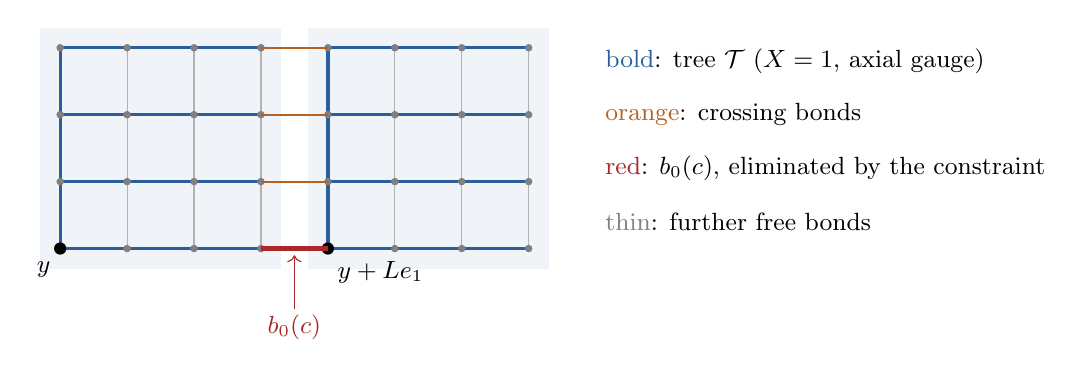
\begin{tikzpicture}[scale=0.85]
\foreach \bx in {0,4} {
  \fill[fblue!7] (\bx-0.3,-0.3) rectangle (\bx+3.3,3.3);
  \foreach \i in {1,...,3} \foreach \j in {0,...,2} \draw[gray!60] (\bx+\i,\j)--(\bx+\i,\j+1);
  \draw[fblue,very thick] (\bx,0)--(\bx,3);
  \foreach \j in {0,...,3} \draw[fblue,very thick] (\bx,\j)--(\bx+3,\j);
  \foreach \i in {0,...,3} \foreach \j in {0,...,3} \fill[gray] (\bx+\i,\j) circle (1.6pt);
  \fill[black] (\bx,0) circle (2.6pt);
}
\foreach \j in {1,...,3} \draw[forange,thick] (3,\j)--(4,\j);
\draw[fred,ultra thick] (3,0)--(4,0);
\node[below left,font=\small] at (0,-0.05) {$y$};
\node[below right,font=\small] at (4,-0.05) {$y+Le_1$};
\draw[fred,->] (3.5,-0.9)--(3.5,-0.1);
\node[below,fred,font=\small] at (3.5,-0.85) {$b_0(c)$};
\node[font=\small,align=left,anchor=west] at (8.0,2.8) {\textcolor{fblue}{bold}: tree $\mathcal T$ ($X=1$, axial gauge)};
\node[font=\small,align=left,anchor=west] at (8.0,2.0) {\textcolor{forange}{orange}: crossing bonds};
\node[font=\small,align=left,anchor=west] at (8.0,1.2) {\textcolor{fred}{red}: $b_0(c)$, eliminated by the constraint};
\node[font=\small,align=left,anchor=west] at (8.0,0.4) {\textcolor{gray}{thin}: further free bonds};
\end{tikzpicture}
\caption{Two blocks $B'(y)$, $B'(y+Le_1)$ of $\T$ for $d=2$, $L=4$. The tree runs first in direction $2$, then in direction $1$.}
\label{fig:tree}
\end{figure}

Let $\mathcal G'=\{u:\T\to G:\ u|_{\T'}=1\}$. By Lemma~\ref{lem:axial}(a), with $h=1$, every $\mathcal G'$-orbit of relative configurations at scale $k$ contains exactly one axial configuration $X^{\rm ax}$. No smallness is needed for this.

\begin{lemma}[Faddeev--Popov identity for the axial gauge]\label{lem:FP}
Let $f$ be an integrable function of configurations on $\T$ with $f(V^u)=f(V)$ for all $u\in\mathcal G'$. Then
\[
\int\prod_bdV(b)\,f(V)=\int\prod_{b\notin\mathcal T}dX(b)\ f(XW)\Big|_{X=1\text{ on }\mathcal T}.
\]
\end{lemma}

\begin{proof}
For a relative configuration $X$, let $g=g(X)\in\mathcal G'$ be the transformation with $X^{(g)}$ axial (Lemma~\ref{lem:axial}(a)). Its value $g(x)$ depends only on $X$ on the tree bonds of $\Gamma^{k+1}_{y,x}$. Hence, for fixed tree variables, the map $(X(b))_{b\notin\mathcal T}\mapsto(X^{(g)}(b))_{b\notin\mathcal T}$ is bondwise a left and right translation, and it preserves the product Haar measure. Since $f((XW)^g)=f(XW)$ and $X^{(g)}=1$ on $\mathcal T$,
\[
\int\prod_bdX(b)\,f(XW)=\int\prod_{b\in\mathcal T}dX(b)\int\prod_{b\notin\mathcal T}dX(b)\,f\big(X^{(g)}W\big)=\int\prod_{b\notin\mathcal T}dX(b)\,f(XW)\Big|_{X=1\text{ on }\mathcal T}.
\]
The tree integrals give $1$, by normalization of the Haar measure.
\end{proof}

\begin{definition}[Fluctuation cutoff]\label{def:chi-w}
For $w\le\frac12c_G$ and a configuration $V$ on $\T$ let $X^{\rm ax}$ be the axial representative of the $\mathcal G'$-orbit of $VW^{-1}$. Put $\chi^{\rm w}(V)=1$ if $|\ell(X^{\rm ax}(b))|\le w$ for all bonds $b$, and $\chi^{\rm w}(V)=0$ otherwise.
\end{definition}

The function $\chi^{\rm w}$ depends on $V'$ through $W$. It is invariant under $\mathcal G'$ by construction. It does not depend on the choice of $U'$ in its orbit. Indeed, replacing $U'$ by $U'^v$ with $v|_{\T'}=1$ replaces $W$ by $W^{v}$ and the axial representative by its transform, whose relative field is $R(v(b_-))X^{\rm ax}(b)$; this has the same norm. Under global gauge transformations $\chi^{\rm w}$ is covariant in the same way.

\subsection{Elimination of the constraint}

For axial $X=e^{\ii Z}$, i.e.\ $Z=0$ on $\mathcal T$, and a bond $c$ of $\T'$ put
\[
\ell_c(Z)=\ell\big(\overline X(c)\big),\qquad\overline X=\mathfrak a'(XW)\,W'^{-1}.
\]
The constraint in \eqref{eq:rg-map} is $\ell_c(Z)=0$ for all $c$. Let $l'=l_{k+1}$ be the linear one-step operator of Lemma~\ref{lem:one-step-expansion} at the background $W$. Let $\mathsf a:=2(C_*+1)\eps'_1$. By Lemma~\ref{lem:composition} and Proposition~\ref{prop:sharp-curvature}, it bounds the curvature both of $W$ and of the fine reference $U'$, in the units of step $k+1$. The latter is what Lemma~\ref{lem:one-step-expansion} needs.

\begin{lemma}[Local elimination]\label{lem:eliminate}
There are $C,c>0$, depending only on $d$ and $G$, such that the following holds with $\rho_L=cL^{-d-1}$ and $r_L=c^2L^{-2d-1}$, provided $L^{d}\mathsf a\le c$. Moreover $d\mathsf a+4dL^2r_L\le\frac12c_G$.
\begin{enumerate}[label=(\alph*)]
\item $\ell_c$ is analytic for complex $Z$ with $|Z|\le cL^{-1}$ on the bonds with both endpoints in $B'(c_-)\cup B'(c_+)$, and depends only on these values. Among the bonds $b_0(c')$ it depends only on $Z(b_0(c))$. Moreover $\ell_c(Z)=L(l'Z)(c)+O(L^2|Z|^2)$.
\item $\partial\ell_c/\partial Z(b_0(c))=L^{1-d}R\big(W([c_-,b_0(c)_-])\big)\big(1+\mathfrak r_c(Z)\big)$ with $|\mathfrak r_c(Z)|\le C(L^d\mathsf a+L^{d+1}|Z|)$.
\item For complex $Z$ on the free bonds with $|Z|\le r_L$ there is exactly one $\zeta_c(Z)$ with $|\zeta_c(Z)|\le\rho_L$ such that $\ell_c=0$ when $Z(b_0(c))=\zeta_c(Z)$. It is analytic, real for real $Z$, depends only on $Z$ on the bonds of (a), and satisfies $|\zeta_c(Z)|\le CL^d\max|Z|$, the maximum running over those bonds.
\item Let $\hat Z(Z)$ be the field equal to $Z$ on $\mathfrak F$, to $\zeta_c(Z)$ on $b_0(c)$ and to $0$ on $\mathcal T$, and write $\hat Z=\hat Z^1Z+\hat Z^2(Z)+\hat Z^{\ge3}(Z)$ (Taylor expansion). Then $\hat Z^1$ is a linear bijection from fields on $\mathfrak F$ onto
\[
\mathcal Z=\{B:\ B=0\text{ on }\mathcal T,\ l'B=0\},
\]
and $\|Z\|\le\|\hat Z^1Z\|\le CL^{d}\|Z\|$. The maps $\hat Z^2$, $\hat Z^{\ge3}$ are supported on the bonds $b_0(c)$ and satisfy $|\hat Z^2(Z)(b_0(c))|\le CL^{3d+1}\max|Z|^2$, the maximum over the bonds of (a).
\end{enumerate}
\end{lemma}

\begin{proof}
(a), (b) For axial $X$ we have $\tau_X=1$, so $\overline X=\tilde{\mathfrak a}_{k+1}(X)$ (Definition~\ref{def:adapted}). We apply Lemma~\ref{lem:one-step-expansion} in the units of step $k+1$. There $\delta_k=L^{-1}$ and $X=e^{\ii\delta_kB}$ with $B=LZ$, so
\[
\ell_c(Z)=(l'B)(c)+c_{k+1}(B)(c)=L(l'Z)(c)+c_{k+1}(LZ)(c),
\]
with the bounds of that lemma for $|B|\le c_2$. This gives (a) and the analyticity, with the bonds stated there.

Next consider the coefficient of $Z(b_0(c))$ in $(q_{k+1}Z)(c)$. The straight contour $[x,x(c)]$ contains $b_0(c)$ if and only if $x$ is one of the points $c_-+me_\mu$, $0\le m<L$. For these $x$ the transport $R(W(\Gamma^{k+1}_{c_-,x}))R(W([x,b_0(c)_-]))$ equals $R(W([c_-,b_0(c)_-]))$, since both paths run along the same line. So the coefficient is $L\cdot L^{-d}L^{-1}R(W([c_-,b_0(c)_-]))$, and in $L(q_{k+1}Z)(c)$ it is $L^{1-d}R(W([c_-,b_0(c)_-]))$. The bound on $r_{k+1}$ in Lemma~\ref{lem:one-step-expansion}(b) and the Lipschitz bound for $c_{k+1}$ in (c), applied to $B=LZ$, change it by at most $CL\mathsf a+CL^2|Z|$, i.e.\ relatively by $C(L^d\mathsf a+L^{d+1}|Z|)$. The factor $L^{d+1}$ is genuine: the coefficient $L^{1-d}$ is what remains after the cancellation of terms of order one between $W([c])$ and the $L^d$ loops, and the non-abelian corrections act on those terms. Here $\mathsf a$ bounds the curvature of the fine reference $U'$ in the units of step $k+1$, as in Lemma~\ref{lem:one-step-expansion}. A bond $b_0(c')$ has both endpoints in $B'(c_-)\cup B'(c_+)$ only if $c'=c$.

(c) Put $M_c=L^{1-d}R(W([c_-,b_0(c)_-]))$ and consider $\Phi(z)=z-M_c^{-1}\ell_c(Z,z)$, where $z$ is the value on $b_0(c)$. By (b), $|\Phi'(z)|\le\frac12$ on $|z|\le\rho_L$ if $c$ is small, since there $L^{d+1}|z|\le c$. By (a), $|\ell_c(Z,0)|\le CL\max|Z|$, so $|\Phi(0)|\le C_0L^d\max|Z|$, with $C_0$ depending only on $d$ and $G$. For $|Z|\le r_L=c^2L^{-2d-1}$ this is at most $C_0c\,\rho_L\le\frac12\rho_L$ for $c\le1/(2C_0)$. (With the same constant $c$ in $\rho_L$ and $r_L$ the contraction would not close.) So $\Phi$ is a contraction of $\{|z|\le\rho_L\}$ into itself, and its fixed point is the unique zero there. Analyticity follows as in Lemma~\ref{lem:linearizing}. Reality follows from uniqueness, since $\overline X\in G$ for real $Z$. Finally, $\mathsf a\le L^{-d}c\le c$ and $L^2r_L\le c^2$, so $d\mathsf a+4dL^2r_L\le dc+4dc^2\le\frac12c_G$ for $c\le c_G/(10d)$.

(d) Differentiating $\ell_c(\hat Z(Z))=0$ at $Z=0$ gives $L(l'\hat Z^1Z)(c)=0$ for all $c$, so $\hat Z^1Z\in\mathcal Z$. Conversely, $B\in\mathcal Z$ is determined by its values on $\mathfrak F$: by (b) at $Z=0$, the equation $(l'B)(c)=0$ fixes $B(b_0(c))$. This gives the bijection. The bound on $\hat Z^1$ follows from $|\zeta^{1}_c(Z)|^2\le CL^{2d}\max|Z|^2\le CL^{2d}\sum|Z(b)|^2$, the sum over the bonds of (a), since each bond lies in a bounded number of these sets. The bound on $\hat Z^2$ follows from Cauchy's estimate, since $|\zeta_c|\le\rho_L$ on $|Z|\le r_L$.
\end{proof}

\subsection{The exact formula}

Let $\sigma$ be the density of the normalized Haar measure in exponential coordinates: $d(e^{\ii Z})=\sigma(Z)\,dZ$ for $|Z|<c_G$, where $dZ$ is the Lebesgue measure on $\mathfrak g$ given by the trace form. It is analytic, positive and $\operatorname{Ad}$-invariant near $0$, and $\sigma(Z)/\sigma(0)=\det\big(\sinh(\tfrac{\ii}{2}\operatorname{ad}Z)/(\tfrac{\ii}{2}\operatorname{ad}Z)\big)=1+O(|Z|^2)$. The $\delta$-function of $G$ is then $\delta(e^{\ii w})=\delta(w)/\sigma(w)$ near $1$.

\begin{proposition}[One step in fluctuation coordinates]\label{prop:exact-step}
Let $V'$ be as in Lemma~\ref{lem:composition}, with $L^d\mathsf a\le c$, and let $w\le r_L$ (so $w\le\rho_L$). Let $\rho$ be gauge invariant, and measurable and bounded on the support of $\chi^{\rm w}$. Then $\chi^{\rm w}$ vanishes outside the interior of $\operatorname{dom}\mathfrak a'$, $\mathfrak a'$ is a submersion at every point where $\chi^{\rm w}=1$, and the density of $T(\chi^{\rm w}\rho)$ at $V'$, defined in Section~\ref{sec:rg-step}, is
\[
T(\chi^{\rm w}\rho)(V')=\int_{(\mathfrak g)^{\mathfrak F}}\prod_{b\in\mathfrak F}\sigma(Z(b))\,dZ(b)\ \ \chi^{\rm w}\big(\hat Z(Z)\big)\prod_c\mathsf J_c(Z)\ \rho\big(e^{\ii\hat Z(Z)}W\big),
\]
where $\chi^{\rm w}(\hat Z)=\prod_b\mathbf 1(|\hat Z(b)|\le w)$ and
\[
\mathsf J_c(Z)=\frac{\sigma(\zeta_c(Z))}{\sigma(0)\,\det\partial\ell_c/\partial Z(b_0(c))}\,,
\]
evaluated at $Z(b_0(c))=\zeta_c(Z)$. For real $Z$ this determinant is positive (see the proof), so it equals its absolute value, which is what the change of variables produces. The integrand is defined to be $0$ if $|Z(b)|>w$ for some $b\in\mathfrak F$. On the remaining set $|Z|_\infty\le w\le r_L$, so $\zeta_c(Z)$, $\hat Z(Z)$, $\mathsf J_c(Z)$ and $\sigma(Z(b))$ are defined, and the factor $\chi^{\rm w}(\hat Z(Z))$ imposes the cutoff also on the bonds $b_0(c)$. The same convention is used for all integrals over fields on $\mathfrak F$ below. Each $\mathsf J_c$ is an analytic function of $Z$ on the bonds of Lemma~\ref{lem:eliminate}(a), and $\mathsf J_c(Z)=L^{(d-1)\dim\mathfrak g}\big(1+O(L^d\mathsf a+L^{2d+1}|Z|_\infty)\big)$, with $|Z|_\infty$ the sup over the free bonds. The value on $b_0(c)$ is $\zeta_c$, with $|\zeta_c|\le CL^d|Z|_\infty$.
\end{proposition}

\begin{proof}
\emph{Domain and submersion.} Let $\chi^{\rm w}(V)=1$, and let $X=e^{\ii Z}$ be the axial representative of Definition~\ref{def:chi-w}. Then $|Z(b)|\le w$ on all bonds, and $V=(XW)^u$ for some $u\in\mathcal G'$. The holonomy $(XW)(\partial p)$ of a plaquette is the product of four unitary conjugates of the $e^{\pm\ii Z(b)}$ and of $W(\partial p)$. By Lemma~\ref{lem:log-estimates}(b) and Lemma~\ref{lem:composition}(a), $XW$, and hence $V$, has curvature at most $L^{-2}\mathsf a+4w$ in the units of step $k$. Since $dL^2(L^{-2}\mathsf a+4w)\le d\mathsf a+4dL^2r_L\le\frac12c_G$ (Lemma~\ref{lem:eliminate}), $V$ lies in the interior of $\operatorname{dom}\mathfrak a'$ (Section~\ref{sec:rg-step}). By Lemma~\ref{lem:eliminate}(a),(b), the derivative of $Z\mapsto(\ell_c(Z))_c$ with respect to the variables $Z(b_0(c))$ is block diagonal, with the invertible blocks $L^{1-d}R(W([c_-,b_0(c)_-]))(1+\mathfrak r_c)$; here $|\mathfrak r_c|\le\frac12$, as in the proof of Lemma~\ref{lem:eliminate}(c), since $|Z|\le w\le\rho_L$. Since $\ell_c(Z)=\ell\big(\mathfrak a'(e^{\ii Z}W)(c)\,V'(c)^{-1}\big)$, and the exponential and the logarithm are local diffeomorphisms, $\mathfrak a'$ is a submersion at $XW$. It is one at $V$ as well, since $\mathfrak a'(Y^u)=\mathfrak a'(Y)$ for $u\in\mathcal G'$.

\emph{The density.} The density at $V'$ is the integral of $\chi^{\rm w}\rho$ over the fibre $\{\mathfrak a'(V)=V'\}$, with respect to the measure induced by the two Haar measures (Section~\ref{sec:rg-step}). We write its computation with $\delta$-functions. The reduction to axial $X$ below is Lemma~\ref{lem:FP} for this fibre integral, with the same proof. For fixed tree variables, the substitution $X\mapsto X^{(g)}$ of that proof is a bondwise translation of the other variables. It preserves their Haar measure, and it does not change $\mathfrak a'$, since $g\in\mathcal G'$. So it maps the part of the fibre with these tree variables onto the axial part of the fibre, with the induced measures, and the integral over the tree variables gives $1$. The elimination of $Z(b_0(c))$ is then the change of variables $z\mapsto\ell_c(Z,z)$ at fixed free variables.

The integrand $\prod_c\delta(\mathfrak a'(V)(c)V'(c)^{-1})\,\chi^{\rm w}(V)\rho(V)$ is invariant under $\mathcal G'$: for $\rho$ by assumption, for $\chi^{\rm w}$ by construction, and for the constraint by Lemma~\ref{lem:one-step-basic}(b). By Lemma~\ref{lem:FP} we may restrict to axial $X$. Then $\chi^{\rm w}$ requires $|\ell(X(b))|\le w$ on all bonds, and on this set $X=e^{\ii Z}$ with $dX(b)=\sigma(Z(b))dZ(b)$. By Lemma~\ref{lem:eliminate}(a), the $\delta$-function for $c$ involves, among the variables $Z(b_0(\cdot))$, only $Z(b_0(c))$. So the integrals over these variables factorize. For fixed free variables, $Z(b_0(c))\mapsto\ell_c$ has at most one zero in $|Z(b_0(c))|\le w$, by Lemma~\ref{lem:eliminate}(c). It is $\zeta_c(Z)$ if $|\zeta_c(Z)|\le w$; otherwise the integrand vanishes, which is accounted for by the factor $\chi^{\rm w}(\hat Z(Z))$. Hence
\[
\int\sigma(z)\,dz\ \delta\big(e^{\ii\ell_c(Z,z)}\big)\,(\cdots)=\int\sigma(z)\frac{\delta(\ell_c(Z,z))}{\sigma(\ell_c(Z,z))}(\cdots)\,dz=\frac{\sigma(\zeta_c)}{\sigma(0)\,|\det\partial_z\ell_c|}(\cdots)\Big|_{z=\zeta_c} .
\]
\emph{Positivity of the determinant.} By Lemma~\ref{lem:eliminate}(b),
\[
\det\partial_z\ell_c=L^{(1-d)\dim\mathfrak g}\det R\big(W([c_-,b_0(c)_-])\big)\det(1+\mathfrak r_c).
\]
Here $\det R(\cdot)=1$ on $\mathfrak g$, since $G$ is connected (Section~\ref{sec:background}). In the proof of Lemma~\ref{lem:eliminate}(c), $|\mathfrak r_c|\le\frac12$ wherever $\zeta_c$ is defined, so $t\mapsto\det(1+t\mathfrak r_c)$ does not vanish on $[0,1]$, and $\det(1+\mathfrak r_c)>0$ for real $Z$. Hence $|\det\partial_z\ell_c|=\det\partial_z\ell_c$ for real $Z$, and $\mathsf J_c$ is the analytic function of the statement. The bound on $\mathsf J_c$ follows from Lemma~\ref{lem:eliminate}(b),(c), since $L^{d+1}|\zeta_c|\le CL^{2d+1}|Z|_\infty$ and $\sigma(\zeta_c)/\sigma(0)=1+O(|\zeta_c|^2)$.
\end{proof}

This is Ba\l aban's representation \cite[(9)--(18)]{BalUV3}, with the elimination performed on one bond per coarse bond, so that the Jacobians are local \cite[(17), (20)]{BalUV3}. It is exact. No small-field approximation has been made beyond the insertion of $\chi^{\rm w}$.

\section{The coarse effective action}\label{sec:coarse-action}

The integrand of Proposition~\ref{prop:exact-step} depends on the fluctuation through the action of the background field, $S(U_k(e^{\ii\hat Z}W))$. In this section we study this function of the coarse configuration. Its gradient is the Lagrange multiplier of the variational problem; its derivatives decay along trees; and its Hessian at the base configuration is comparable with the operator $\boldsymbol\Gamma_\pi-a$ of Part~II.

\paragraph{Setting.} In this section $k\ge1$: the $k$-step operators of Parts~II--V at $U'$ need at least one averaging step (Section~\ref{sec:setup}). The first step, $k=0$, is treated in Remark~\ref{rem:step-k0}. Let $W$ be a real configuration on $\T$ in $\mathfrak U_k(\eps_1)$, $\eps_1\le a_1$, and let $U'$ be an element of its minimal orbit. Let $\eps$ be a number such that $U'$ is $(M,\eps)$-regular with $|J_{U'}|\le\eps$; by Theorem~\ref{thm:balaban} one may take $\eps=B_3\eps_1$, and in Section~\ref{sec:fluctuations} we take $\eps=B_3\eps'_1$ (end of Section~\ref{sec:rg-step}). We assume $\eps\le c_6/2$, and we put $r_1:=c_6/4$. In Section~\ref{sec:fluctuations}, $W$ is the base configuration $V^0$ and $U'$ the $(k+1)$-step background. For complex unit-lattice fields $B$ with $|B|_\infty<2r_1$, so that $\eps+|B|_\infty<c_6$, let $A_*(B)$ be the Landau representative relative to $U'$ given by Theorem~\ref{thm:variational}(f), for the coarse configuration $e^{\ii B}W$, and put
\[
\mathcal S(B)=\Phi\big(A_*(B)\big),\qquad\Phi(A)=S(e^{\ii\eta A}U').
\]
The bounds of Proposition~\ref{prop:coarse-action}(c) are stated on the smaller ball $|B|_\infty<r_1$. The margin $r_1$ between the two balls is used only for Cauchy's estimate in the proof of the third-derivative bound. For real $B$, $\mathcal S(B)$ is the minimum of $S$ on $\mathfrak B(e^{\ii B}W)\cap\mathfrak U(\theta_0)$: by Theorem~\ref{thm:variational}(a),(b) the orbit of $\mathsf U(A_*(B))$ is the set of minimizers there, and $S(\mathsf U(A))=\Phi(A)$. If moreover $e^{\ii B}W\in\mathfrak U_k(a_1)$, this orbit is the minimal orbit of Theorem~\ref{thm:balaban}(a), and $\mathcal S(B)=S(U_k(e^{\ii B}W))$; this is the case in all uses below. In particular $\mathcal S$ depends only on the configuration $e^{\ii B}W$, and not on the choice of the reference $U'$.

For bonds $c_1,\dots,c_m$ of $\T$ let $\tau(c_1,\dots,c_m)=\min_{z}\sum_i|c_i-z|$; for $m=2$ this is $|c_1-c_2|$. It satisfies $\tau(c_1,\dots,c_m)\le|c_1-x|+\tau(x,c_2,\dots,c_m)$.

\subsection{Gradient and decay of derivatives}

\begin{proposition}[The coarse effective action]\label{prop:coarse-action}
There are $C,\gamma_1>0$, independent of $k$, $n$, $\eta$ and $W$, such that:
\begin{enumerate}[label=(\alph*)]
\item $\mathcal S$ is analytic on $\{|B|_\infty<2r_1\}$ and real for real $B$.
\item $\nabla\mathcal S(B)=\omega(B)$, where for real $B$, $\omega(B)$ is the multiplier of Proposition~\ref{prop:euler-lagrange} for the coarse configuration $e^{\ii B}W$; $\omega$ is analytic, and $|\omega(B)|_\infty\le C(\eps+|B|_\infty)$ for $|B|_\infty<2r_1$.
\item For $|B|_\infty<r_1$ and all bonds $c_1,c_2,c_3$:
\[
|\partial_{c_1}\partial_{c_2}\mathcal S(B)|\le Ce^{-\gamma_1|c_1-c_2|},\qquad|\partial_{c_1}\partial_{c_2}\partial_{c_3}\mathcal S(B)|\le Ce^{-\gamma_1\tau(c_1,c_2,c_3)},
\]
where $\partial_c$ is the derivative with respect to $B(c)$, the components being suppressed.
\item Put $\omega_0=\omega(0)$ and $\Delta^0=d^2\mathcal S(0)$. For $|B|_\infty\le r_1/2$,
\[
\mathcal S(B)=\mathcal S(0)+\ip{\omega_0}B+\tfrac12\Delta^0(B,B)+\mathcal S_3(B),\qquad|\mathcal S_3(B)|\le C|B|_\infty\|B\|^2 .
\]
\end{enumerate}
\end{proposition}

\begin{proof}
(a) $A_*$ is analytic with $|A_*(B)|_{C^1}\le C_6(\eps+|B|_\infty)\le c_5$, and $\Phi$ is analytic there (Proposition~\ref{prop:action}).

(b) For real $B$, Proposition~\ref{prop:euler-lagrange} gives $\nabla\Phi(A_*(B))=d\mathcal Q(A_*(B))^T\omega(B)$. Differentiating the constraint $\ell(\mathcal Q(e^{\ii\eta A_*(B)}))=B$ gives $d\mathcal Q(A_*)\,dA_*(B)=I$. Hence
\[
d\mathcal S(B)h=\ip{\nabla\Phi(A_*)}{dA_*h}=\ip{\omega}{d\mathcal Q(A_*)dA_*h}=\ip\omega h .
\]
Applying $\bH^T$ to the Euler--Lagrange equation gives
\[
\omega(B)=\big((I+dC_k(A_*)\bH)^{-1}\big)^T\bH^T\nabla\Phi(A_*(B)).
\] This expression is analytic in complex $B$ and defines the continuation of $\omega$. The identities $\nabla\Phi(A_*)=d\mathcal Q(A_*)^T\omega$ and $\nabla\mathcal S=\omega$ hold for real $B$, hence for complex $B$ by the identity theorem: the real ball is a totally real submanifold of maximal dimension. The bound for real $B$ is Proposition~\ref{prop:euler-lagrange}; for complex $B$ it follows from the formula, Lemma~\ref{lem:sup-bounds}, Proposition~\ref{prop:action}(a), and the identity $\bH^TD^TDA_*=(\boldsymbol\Gamma_\pi-a)\bQ A_*$. This is the second identity in the proof of Lemma~\ref{lem:V-bounds}; it applies since $RD^TA_*=RD^TA'_*=0$ also for complex $B$ (Lemma~\ref{lem:linearizing}, $A'_*\in\bH B+\cX$). The bound $|A_*|_{C^1}\le C(\eps+|B|_\infty)$ alone would not bound $D^TDA_*$ pointwise.

(c) \emph{Second derivatives.} We prove the bound on the larger ball $|B|_\infty<2r_1$. Let $|B|_\infty<2r_1$. Differentiating $d\mathcal S(B)h=\ip{\nabla\Phi(A_*)}{dA_*h}$ once more,
\[
d^2\mathcal S(B)[h_1,h_2]=d^2\Phi(A_*)[dA_*h_1,dA_*h_2]-\ip{\omega}{d^2C_k(A_*)[dA_*h_1,dA_*h_2]},
\]
where we used $\ip{\nabla\Phi}{d^2A_*[h_1,h_2]}=\ip\omega{d\mathcal Q\,d^2A_*[h_1,h_2]}$ and the second derivative of the constraint, $d\mathcal Q\,d^2A_*[h_1,h_2]+d^2C_k(A_*)[dA_*h_1,dA_*h_2]=0$. Now:
\begin{itemize}
\item $d^2\Phi(A)=D^TD+d^2\mathcal N(A)$, where $d^2\mathcal N(A)$ is a sum of plaquette-local terms with bounded coefficients (proof of Proposition~\ref{prop:action}(c));
\item $d^2C_k(A)[u,v](c)$ is bounded by $C\|u\|_{S_c}\|v\|_{S_c}$, by polarization of Proposition~\ref{prop:Q-expansion}(c);
\item by Theorem~\ref{thm:variational}(f), which holds for complex $B$ with $\eps+|B|_\infty<c_6$, and here $\eps+|B|_\infty<2r_1+2r_1=c_6$: $|dA_*\delta_{c_i}|+|\nabla dA_*\delta_{c_i}|\le Ce^{-\gamma'|x-c_i|}$.
\end{itemize}
Hence $|\partial_{c_1}\partial_{c_2}\mathcal S(B)|\le C\sum_xe^{-\gamma'(|x-c_1|+|x-c_2|)}\eta^d\le Ce^{-\gamma'|c_1-c_2|/2}$ for $|B|_\infty<2r_1$.

\emph{Third derivatives.} Let $|B|_\infty<r_1$, and let $e$ be a unit vector of $\mathfrak g$. For complex $t$ with $|t|<2r_1-|B|_\infty$ we have $|B+te\,\delta_{c_3}|_\infty<2r_1$. Since $2r_1-|B|_\infty>r_1$, the function $t\mapsto\partial_{c_1}\partial_{c_2}\mathcal S(B+te\,\delta_{c_3})$ is analytic on a neighbourhood of the closed disc $|t|\le r_1$, and, by the bound just proved on the larger ball, it is bounded there by $Ce^{-\gamma'|c_1-c_2|/2}$. By Cauchy's estimate on the circle $|t|=r_1$,
\[
|\partial_{c_1}\partial_{c_2}\partial_{c_3}\mathcal S(B)|\le Cr_1^{-1}e^{-\gamma'|c_1-c_2|/2}.
\]
The left side is symmetric in $c_1,c_2,c_3$. So the bound holds with $|c_1-c_2|$ replaced by the largest distance $D$ between two of the three bonds. Taking $z=c_1$ in the definition of $\tau$ gives $\tau(c_1,c_2,c_3)\le|c_2-c_1|+|c_3-c_1|\le2D$. This proves (c) with $\gamma_1=\gamma'/4$. No bound on the second or higher derivatives of $A_*$ on the fine lattice is used.

(d) Fix $B$ and a bond $c$, and let $R(s)=\omega(sB)(c)$ for complex $s$ with $|s|\,|B|_\infty<r_1$. By (c), $|R'(s)|=|d\omega(sB)B(c)|\le C\sum_{c'}e^{-\gamma_1|c-c'|}|B(c')|=:K_c$ on this disc. By the Schwarz lemma applied to $R'(s)-R'(0)$, $|R'(s)-R'(0)|\le4K_c|B|_\infty r_1^{-1}$ for $|s|\le1$, when $|B|_\infty\le r_1/2$. By (b),
\[
\mathcal S_3(B)=\int_0^1\ip{\omega(tB)-\omega_0-t\,d\omega(0)B}B\,dt,\qquad|\mathcal S_3(B)|\le C|B|_\infty\sum_c K_c|B(c)|\le C|B|_\infty\|B\|^2,
\]
by the Schur test.
\end{proof}

Part (b) is the discrete form of the statement that the derivative of the minimal action with respect to the constraint is the Lagrange multiplier. Part (c) is what makes the coarse action, and the Gaussian measure it defines, local.

\subsection{The Hessian at the base configuration}

Recall that $\bH=\bH(U')$, $\cX=\{A:RD^TA=0,\ \bQ A=0\}$ and $\boldsymbol\Gamma_\pi=\boldsymbol\Gamma_\pi(U')$ are taken at $U'$ with the averaging pair $(Q'_k(U'),\bQ_k(U'))$, and that
\begin{equation}\label{eq:H-effective}
\bH^TD^TD\bH=\boldsymbol\Gamma_\pi-a .
\end{equation}
This follows from the first identity in the proof of Lemma~\ref{lem:V-bounds} and $S\bH=G'RD^T\bH=0$. At $U'=1$ the right-hand side is the operator $\bD$ of Proposition~\ref{prop:eff-action-gauge}.

\begin{proposition}[The Hessian]\label{prop:hessian}
\begin{enumerate}[label=(\alph*)]
\item For real $B$,
\[
\Delta^0(B,B)=\min\big\{q_2(A,A):\ \bQ A=B,\ RD^TA=0\big\},
\]
\[
q_2(A,A)=\|DA\|^2+d^2\mathcal N(0)[A,A]-\ip{\omega_0}{d^2C_k(0)[A,A]},
\]
and the minimum is attained at $A=dA_*(0)B$.
\item $\big|\Delta^0(B,B)-\ip B{(\boldsymbol\Gamma_\pi-a)B}\big|\le C\eps\|B\|^2$.
\item $\Delta^0$ is real symmetric with decay $(C,\gamma_1)$.
\item For every real gauge transformation $u$ on $\Tf$, replacing $(W,U')$ by $(W^{u|_\T},U'^u)$ replaces $\Delta^0$ by $R(u)\Delta^0R(u)^{-1}$ and $\omega_0$ by $R(u)\omega_0$, where $R(u)$ acts on unit-lattice fields by $R(u(b_-))$.
\end{enumerate}
\end{proposition}

\begin{proof}
(a) Let $A^1$ satisfy $\bQ A^1=B$ and $RD^TA^1=0$. Put $A(t)=tA^1-\bH\mathcal D(tA^1)$. By Lemma~\ref{lem:linearizing}, $RD^TA(t)=0$ and $\ell(\mathcal Q(e^{\ii\eta A(t)}))=tB$. Moreover $\mathcal D(tA^1)=t^2C^{(2)}_k(A^1)+O(t^3)$, where $C^{(2)}_k(A)=\frac12d^2C_k(0)[A,A]$. For real $t$ near $0$ the configuration $\mathsf U(A(t))$ lies in $\mathfrak B(e^{\ii tB}W)\cap\mathfrak U(\theta_0)$. By Theorem~\ref{thm:variational}(b), $\mathcal S(tB)\le\Phi(A(t))$. Expand $\Phi$ with Proposition~\ref{prop:action}:
\[
\Phi(A(t))=\mathcal S(0)+t\ip J{A^1}+t^2\Big(\tfrac12\|DA^1\|^2+\tfrac12d^2\mathcal N(0)[A^1,A^1]-\ip J{\bH C^{(2)}_k(A^1)}\Big)+O(t^3),
\]
with $J=J_{U'}=\nabla\Phi(0)=\bQ^T\omega_0$. Then $\ip J{A^1}=\ip{\omega_0}B$ and $\ip J{\bH C^{(2)}_k(A^1)}=\ip{\omega_0}{C^{(2)}_k(A^1)}$, since $\bQ\bH=I$. The terms of first order agree with those of $\mathcal S(tB)$. So the inequality for $t\to0$ gives $\Delta^0(B,B)\le q_2(A^1,A^1)$.

For equality, expand $\mathcal S(tB)=\Phi(A_*(tB))$ directly. We have $A_*(tB)=tA^1+t^2A^2+O(t^3)$ with $A^1=dA_*(0)B$, both in the slice, and the constraint gives $\bQ A^1=B$, $\bQ A^2+C^{(2)}_k(A^1)=0$. Hence the coefficient of $t^2$ is $\frac12\|DA^1\|^2+\frac12d^2\mathcal N(0)[A^1,A^1]+\ip J{A^2}$, and $\ip J{A^2}=\ip{\omega_0}{\bQ A^2}=-\ip{\omega_0}{C^{(2)}_k(A^1)}$. So $\Delta^0(B,B)=q_2(A^1,A^1)$.

(b) Write $A=\bH B+h$ with $h\in\cX$. Then $\|DA\|^2=\|D\bH B\|^2+\|Dh\|^2$, since $\ip{Dh}{D\bH B}=0$ for $h\in\cX$, and $\|D\bH B\|^2=\ip B{(\boldsymbol\Gamma_\pi-a)B}$ by \eqref{eq:H-effective}. By Proposition~\ref{prop:action}(c) at $A=0$, $|d^2\mathcal N(0)[A,A]|\le C\eps(\|A\|^2+\|\nabla A\|^2)$. By Proposition~\ref{prop:Q-expansion}(c) and $|\omega_0|\le C\eps$, $|\ip{\omega_0}{d^2C_k(0)[A,A]}|\le C\eps\|A\|^2$. Moreover:
\begin{itemize}
\item $\|\bH B\|+\|\nabla\bH B\|\le C\|B\|$, by the decay of $\bH$ and $D\bH$, the identity $D^T\bH B=P_\cV D^T\bH B$, and Lemma~\ref{lem:weitzenbock};
\item $\|h\|^2+\|\nabla h\|^2\le c_X^{-1}\|Dh\|^2$, by Lemma~\ref{lem:X-coercive}.
\end{itemize}
Hence
\[
\ip B{(\boldsymbol\Gamma_\pi-a)B}-C\eps\|B\|^2+(1-C\eps)\|Dh\|^2\le q_2(A,A).
\]
Taking the minimum over $h$ gives the lower bound; $h=0$ gives the upper bound.

(c) is Proposition~\ref{prop:coarse-action}(c) at $B=0$. (d) follows from the covariance of the variational problem, Theorem~\ref{thm:variational}(g), and $\mathcal S$ depending only on $e^{\ii B}W$: $(e^{\ii B}W)^{u|_\T}=e^{\ii R(u)B}W^{u|_\T}$.
\end{proof}

\subsection{Dependence on the base configuration}

Let $\hat\beta$ be a complex unit-lattice field with $|\hat\beta|_\infty\le r_1/4$, and $\hat W=e^{\ii\hat\beta}W$ (bondwise product). For real $\hat\beta$ we have $\mathcal S_{\hat W}(B)=\mathcal S_W(B\star\hat\beta)$, with $B\star\hat\beta=\ell(e^{\ii B}e^{\ii\hat\beta})$ bondwise. We use this formula as the definition for complex $\hat\beta$. It defines $\mathcal S_{\hat W}$ analytically in $(\hat\beta,B)$ for $|B|_\infty\le r_1/4$, and in particular $\omega_0(\hat W)$ and $\Delta^0(\hat W)$.

\begin{proposition}[Dependence on the base]\label{prop:base-dependence}
$\omega_0(\hat W)$ and $\Delta^0(\hat W)$ are analytic in $\hat\beta$. Their derivatives with respect to $\hat\beta(c)$ satisfy
\[
|\partial_{\hat\beta(c)}\omega_0(\hat W)(c_1)|\le Ce^{-\gamma_1|c-c_1|},\qquad|\partial_{\hat\beta(c)}\Delta^0(\hat W)(c_1,c_2)|\le Ce^{-\gamma_1\tau(c,c_1,c_2)} .
\]
\end{proposition}

\begin{proof}
$\omega_0(\hat W)=\partial_B\mathcal S_W(B\star\hat\beta)|_{B=0}$ and $\Delta^0(\hat W)=\partial^2_B\mathcal S_W(B\star\hat\beta)|_{B=0}$. The map $(B,\hat\beta)\mapsto B\star\hat\beta$ is bondwise analytic. Its derivatives in $B$ at $B=0$ are bondwise analytic functions of $\hat\beta$. The chain rule expresses the derivatives in terms of $d^m\mathcal S_W(\hat\beta)$, $m\le3$, contracted with bondwise factors. Proposition~\ref{prop:coarse-action}(c) at $B=\hat\beta$, with $|\hat\beta|_\infty\le r_1/4<r_1$, gives the bounds.
\end{proof}

Proposition~\ref{prop:base-dependence} controls the dependence on small changes of the base configuration. Changes that are not small, for example replacing the configuration far away by a different one, require a representation of the operators by terms that depend on the background only locally. This is the random-walk expansion of Section~\ref{sec:random-walk}, which will be developed for the present operators in the next part.

\section{The fluctuation covariance and the step}\label{sec:covariance}

We return to the setting of Section~\ref{sec:fluctuations}: $W=V^0$ is the base configuration of the step, $U'=U_{k+1}(V')$, and $\eps=B_3\eps'_1$. The objects of Section~\ref{sec:coarse-action} are taken at this $W$ and $U'$.

\subsection{The quadratic form of the step}

\begin{lemma}[Expansion in the free variables]\label{lem:step-quadratic}
Let $r_2=\min(cL^{-2d-2},\,cL^{-d}a'_1)$ with $c>0$ small, depending only on $d$, $G$, $L$ and $r_1=c_6/4$ of Proposition~\ref{prop:coarse-action} (the proof needs $2cL^{-2d-2}\le\frac12r_L$, $CL^{-d-2}c\le\frac14r_1$ and $Cc\le\frac12$), $a'_1$ as in Lemma~\ref{lem:composition}(c), and assume $4(C_*+1)L^{-2}\eps'_1\le a'_1$. For complex fields $Z$ on $\mathfrak F$ with $|Z|_\infty\le r_2$ put $F(Z)=\mathcal S(\hat Z(Z))$. Then $F$ is analytic, $F(Z)=S(U_k(e^{\ii\hat Z(Z)}W))$ for real $Z$, and
\[
F(Z)=S(U')+\tfrac12\Delta_k(Z,Z)+\mathcal V(Z),\qquad\Delta_k(Z,Z)=\Delta^0(\hat Z^1Z,\hat Z^1Z)+2\ip{\omega_0}{\hat Z^2(Z)},
\]
with $|\mathcal V(Z)|\le C_L|Z|_\infty\|Z\|^2$. In particular $F$ has no linear term.
\end{lemma}

\begin{proof}
By Lemma~\ref{lem:eliminate}, $\hat Z$ is analytic on $|Z|_\infty\le2r_2\le r_L$ with $|\hat Z(Z)|_\infty\le CL^d|Z|_\infty\le r_1/2$, so $F$ is analytic on the disc of radius $2r_2$ by Proposition~\ref{prop:coarse-action}(a). For real $Z$ the configuration $e^{\ii\hat Z(Z)}W$ satisfies the one-step constraint, and its curvature is at most $2(C_*+1)L^{-2}\eps'_1+CL^dr_2\le a'_1$. Here $|\hat Z|_\infty\le CL^d|Z|_\infty$, so $CL^dr_2\le a'_1/2$ by the choice of $r_2$, and we assume $4(C_*+1)L^{-2}\eps'_1\le a'_1$. By Lemma~\ref{lem:composition}(c), $F(Z)\ge F(0)=S(U')$, so $dF(0)=\ip{\omega_0}{\hat Z^1\cdot}=0$. The second-order term follows from $\hat Z(tZ)=t\hat Z^1Z+t^2\hat Z^2(Z)+O(t^3)$ and Proposition~\ref{prop:coarse-action}(d). For the remainder, $\nabla F(Z)=d\hat Z(Z)^T\omega(\hat Z(Z))$. The analyticity of $\hat Z$ and the bound $|\hat Z(Z)|_\infty\le r_1/2$ hold on the larger disc $|Z|_\infty\le2cL^{-2d-2}$, since only the first term of the minimum defining $r_2$ enters them. By Proposition~\ref{prop:coarse-action}(c) and the locality of $\hat Z$ (range $2L$), $d^2F$ has a kernel bounded by $C_Le^{-\gamma_1|b-b'|}$ on this larger disc. The argument of Proposition~\ref{prop:coarse-action}(d), applied to $F$ on this disc with $dF(0)=0$, gives the bound on $\mathcal V$. Its constant $C_L$ depends on $cL^{-2d-2}$, but not on $a'_1$.
\end{proof}

This is the quadratic form \cite[(53)--(54)]{BalUV3}. The term $2\ip{\omega_0}{\hat Z^2}$ comes from the curvature of the constraint set and is Ba\l aban's term $-\ip{H_1\hat D^{(2)}(A)}J$.

\subsection{Coercivity}

The lower bound for $\Delta_k$ is proved in two steps:
\begin{itemize}
\item at the trivial background, a Poincar\'e inequality on the one-step constraint set combined with Proposition~\ref{prop:eff-action-gauge};
\item at a regular background, an IMS localization on the unit lattice, as in Section~\ref{sec:reg-gauge}.
\end{itemize}
Let $q$ be the one-step tube average at the trivial background, i.e.\ $l'$ with $W=1$.

\begin{lemma}[Poincar\'e inequality for one step]\label{lem:poincare-step}
There is $C_{\rm P}$, depending only on $d$ and $L$, such that every real field $B$ on the bonds of $\T$ with $B=0$ on $\mathcal T$ satisfies
\[
\|B\|^2\le C_{\rm P}\big(\|\dl B\|^2+\|qB\|^2\big),
\]
where $\dl B$ is the unit-lattice curl.
\end{lemma}

\begin{proof}
All estimates are local in a pair of neighbouring blocks.

\emph{Bonds inside a block.} Let $b=(x,x')$ be a bond of $B'(y)$ not in $\mathcal T$. By Lemma~\ref{lem:stokes}(ii) the loop $\Gamma^{k+1}_{y,x}\cup b\cup(\Gamma^{k+1}_{y,x'})^{-1}$ is spanned by at most $dL$ plaquettes. Since $B=0$ on the tree, the abelian Stokes formula gives $B(b)=\sum_i\pm\dl B(p_i)$, so $|B(b)|^2\le dL\sum_i|\dl B(p_i)|^2$.

\emph{Crossing bonds.} Let $c=(y,y')$, $y'=y+Le_\mu$, and for $x$ in the face $\mathsf F=\{x\in B'(y):x_\mu=y_\mu+L-1\}$ let $b_x=(x,x+e_\mu)$. For $x,\tilde x\in\mathsf F$ the closed contour
\[
\Gamma^{k+1}_{y,x}\,b_x\,(\Gamma^{k+1}_{y',x+e_\mu})^{-1}\,\Gamma^{k+1}_{y',\tilde x+e_\mu}\,b_{\tilde x}^{-1}\,(\Gamma^{k+1}_{y,\tilde x})^{-1}
\]
lies in a box of side $2L$ and has at most $4dL+2$ bonds. By Lemma~\ref{lem:stokes}(iii) it is spanned by at most $12d^2L^2$ plaquettes, so $B(b_x)-B(b_{\tilde x})$ is a sum of at most $12d^2L^2$ values $\pm\dl B(p)$.

\emph{The average.} $(qB)(c)=L^{-d}\sum_{x\in B'(y)}L^{-1}B([x,x(c)])$. Each straight contour $[x,x(c)]$ contains exactly one crossing bond $b_{\tilde x}$, with $\tilde x\in\mathsf F$ on the same line as $x$, and $L-1$ bonds inside the two blocks. Each $\tilde x$ occurs for $L$ values of $x$. Hence the mean $m_c$ of $B(b_{\tilde x})$ over $\tilde x\in\mathsf F$ satisfies $|m_c|\le L|(qB)(c)|+(L-1)\max|B(b)|$, the maximum running over the inner bonds of the two blocks. Then $|B(b_x)|\le|m_c|+\max_{\tilde x}|B(b_x)-B(b_{\tilde x})|$.

Squaring and summing, each plaquette and each value $(qB)(c)$ is used a number of times bounded in terms of $d$ and $L$.
\end{proof}

\begin{lemma}[Local comparison]\label{lem:local-comparison}
Let $M'\ge\max(M,L)$ be an integer and $z$ a point of the torus (not necessarily of $\T$). Assume $n\ge80M'$ and $\eps\le\eps_{\rm cmp}(M')$, where $\eps_{\rm cmp}(M')>0$ depends only on $M'$, $d$, $L$, $G$, $a$, $\alpha$ and $M$, and is fixed in the proof. There are a real gauge transformation $u$ on $\Lam_{40M'}(z)$ and $C_{M'}$ such that, for every real field $B$ on the bonds of $\T$ starting in $\Lam_{M'}(z)$ and vanishing on $\mathcal T$, with $B^u=R(u)B$:
\[
\big|\ip B{(\boldsymbol\Gamma_\pi-a)B}-\ip{B^u}{\bD B^u}\big|\le\big(C_{M'}\eps+Ce^{-\gamma M'}\big)\|B\|^2,\qquad\big|\|l'B\|-\|qB^u\|\big|\le C_{M'}\eps\|B\| .
\]
Here $\bD=\boldsymbol\Gamma(1)-a$ is the operator of Proposition~\ref{prop:eff-action-gauge}, and $C,\gamma$ do not depend on $M'$.
\end{lemma}

\begin{proof}
The configuration $U'$ is $3\eps$-regular on every cube $\Lam_{4M+2}(z'')$ (Section~\ref{sec:local-gauges}). Let $z_0\in\Tf$ with $|z-z_0|_\infty\le\eta$, so that $\Lam_{40M'}(z)\subset\Lam_{40M'+1}(z_0)$. Apply Lemma~\ref{lem:large-cubes} with $r=4M+2\ge18$, $R=40M'+1$ and $\sigma=3\eps$, on the cube $\Lam_R(z_0)$. Its hypothesis $C_E(R/r)^pR\sigma\le1$ is the first condition defining $\eps_{\rm cmp}(M')$. The boxes in its proof have sides at most $3R=120M'+3<80M'L\le Ln$, the side of $\T$, so they do not wrap around the torus. This gives a real gauge $u$ on $\Lam_{40M'}(z)$ with $U'^u=e^{\ii\eta A}$ and $\|A\|_{1,\alpha}\le C(40M'/M)^p\eps$. Extend $u$ to a real gauge transformation $\tilde u$ of $\Tf$. Then $\boldsymbol\Gamma_\pi(U'^{\tilde u})=R(\tilde u)\boldsymbol\Gamma_\pi(U')R(\tilde u)^{-1}$ and $l'(W^{\tilde u})R(\tilde u)=R(\tilde u)l'(W)$, by Proposition~\ref{prop:linearized-averages}(f), Proposition~\ref{prop:covariance} and Lemma~\ref{lem:one-step-basic}(b).

Let $\chi$ be a smooth cutoff equal to $1$ on $\Lam_{20M'}(z)$ and $0$ outside $\Lam_{30M'}(z)$, and put $U^\natural=e^{\ii\eta\chi A}$. It satisfies (B) with parameter $C_{M'}\eps$. The second condition defining $\eps_{\rm cmp}(M')$ is that $C_{M'}\eps$ lies below the thresholds of Parts~II and~III. The configuration $U^\natural$ coincides with $U'^{\tilde u}$ on $\Lam_{20M'}(z)$. By Theorem~\ref{thm:reg-locality}(b), the kernels of $\boldsymbol\Gamma_\pi(U'^{\tilde u})$ and $\boldsymbol\Gamma_\pi(U^\natural)$ on $\Lam_{M'}(z)$ differ by at most $C\sum_{w}e^{-\gamma(|y-w|+|w-y'|)}$, summed over $w$ within $10M$ of the complement of $\Lam_{20M'}(z)$. These $w$ are at distance at least $9M'$ from $\Lam_{M'}(z)$, which gives the error $Ce^{-\gamma M'}$ after a Schur bound.

By Part~II at the background $U^\natural$, with the averaging pair $(Q'_k(U^\natural),\bQ_k(U^\natural))$ (Remark~\ref{rem:general-averaging}), $\boldsymbol\Gamma_\pi(U^\natural)-\boldsymbol\Gamma(1)$ has decay $(C_{M'}\eps,\gamma)$. This follows from Theorem~\ref{thm:cov-min}(a) and Lemma~\ref{lem:perturbed-inverse}.

Finally, by Lemma~\ref{lem:avg-local-gauge}, whose hypotheses are the third condition defining $\eps_{\rm cmp}(M')$, $W^{\tilde u}=e^{\ii B_W}$ near $\Lam_{M'}(z)$ with $|B_W|\le C_{M'}\eps$. So the transports in $l'(W^{\tilde u})$ are within $C_{M'}\eps$ of $1$ there. Together with Lemma~\ref{lem:one-step-expansion}(b), this gives $|l'(W^{\tilde u})B^u-qB^u|\le C_{M'}\eps\|B\|$.
\end{proof}

\begin{theorem}[Coercivity on the constraint set]\label{thm:step-coercive}
There are $c_L>0$, depending only on $d$ and $L$, and $M'_L\ge M$ and $\eps_L>0$, depending only on $d$, $L$, $G$, $a$, $\alpha$ and $M$, such that, if $\eps\le\eps_L$ and $n\ge n_0$ with $n_0\ge80M'_L$,
\[
\ip B{(\boldsymbol\Gamma_\pi-a)B}\ge c_L\|B\|^2\qquad\text{for all real }B\in\mathcal Z.
\]
\end{theorem}

\begin{proof}
Let $\{\chi_j\}$ be the partition of Lemma~\ref{lem:partition} at scale $M'$, restricted to the unit lattice, acting on bond fields through $b_-$. The operator $K=\boldsymbol\Gamma_\pi-a$ is bounded with decay $(C,\gamma)$ (Theorem~\ref{thm:reg-min}). By Lemma~\ref{lem:IMS} and the argument of Lemma~\ref{lem:double-comm} for kernels, $\sum_j(\chi_j(x)-\chi_j(x'))^2|K(x,x')|\le CM'^{-2}|x-x'|^2|K(x,x')|$, so
\[
\ip BKB\ge\sum_j\ip{\chi_jB}{K\chi_jB}-CM'^{-2}\|B\|^2 .
\]
Each $\chi_jB$ vanishes on $\mathcal T$ and is supported on bonds starting in a cube of side $2M'$. By Lemma~\ref{lem:local-comparison}, Proposition~\ref{prop:eff-action-gauge} and Lemma~\ref{lem:poincare-step},
\[
\begin{aligned}
\ip{\chi_jB}{K\chi_jB}&\ge c_D\|\dl(\chi_jB)^{u_j}\|^2-\delta_1\|\chi_jB\|^2\\
&\ge c_DC_{\rm P}^{-1}\|\chi_jB\|^2-c_D\|q(\chi_jB)^{u_j}\|^2-\delta_1\|\chi_jB\|^2,
\end{aligned}
\]
with $\delta_1=C_{M'}\eps+Ce^{-\gamma M'}$. Moreover $\|q(\chi_jB)^{u_j}\|^2\le2\|l'\chi_jB\|^2+2C_{M'}^2\eps^2\|\chi_jB\|^2$. The operator $l'$ has range $2L$, and $|\chi_j(x)-\chi_j(x')|\le CL/M'$ within this range. With the bounded overlap of the $\chi_j$, this gives $\sum_j\|l'\chi_jB\|^2\le2\|l'B\|^2+C(L/M')^2\|B\|^2$. For $B\in\mathcal Z$, $l'B=0$. Summing over $j$ with $\sum_j\|\chi_jB\|^2=\|B\|^2$,
\[
\ip BKB\ge\Big(c_DC_{\rm P}^{-1}-CM'^{-2}-Cc_DL^2M'^{-2}-Ce^{-\gamma M'}-C_{M'}\eps\Big)\|B\|^2 .
\]
Choose $M'=M'_L$ so large that the terms independent of $\eps$ are at most $\frac14c_DC_{\rm P}^{-1}$. Then choose $\eps_L\le\eps_{\rm cmp}(M'_L)$, below the threshold of Corollary~\ref{cor:parts-apply} for Theorem~\ref{thm:reg-min} (which gives the decay of $K$ used in the IMS step), so small that $C_{M'_L}\eps_L\le\frac14c_DC_{\rm P}^{-1}$, and put $c_L=\frac12c_DC_{\rm P}^{-1}$. Lemma~\ref{lem:local-comparison} applies, since $n\ge80M'_L$ and $\eps\le\eps_{\rm cmp}(M'_L)$.
\end{proof}

\subsection{The fluctuation covariance}

\begin{corollary}[Fluctuation covariance]\label{cor:covariance}
Let $\eps\le\eps_L$ and $CL^{3d+1}\eps\le\frac14c_L$. Then $\Delta_k$, as an operator on real fields on $\mathfrak F$, is symmetric with
\[
\tfrac14c_L\|Z\|^2\le\Delta_k(Z,Z)\le C_L\|Z\|^2 .
\]
It has decay $(C_L,\gamma_1)$, and $C_k=\Delta_k^{-1}$ has decay $(C'_L,\gamma_C)$. For complex base configurations $\hat W=e^{\ii\hat\beta}W$ with $|\hat\beta|_\infty\le c'_L$, where $c'_L\le r_1/4$ is a small constant, define
\[
\Delta_k(\hat W)(Z,Z)=\Delta^0(\hat W)\big(\hat Z^1_{\hat W}Z,\hat Z^1_{\hat W}Z\big)+2\ip{\omega_0(\hat W)}{\hat Z^2_{\hat W}(Z)},
\]
with the objects of Proposition~\ref{prop:base-dependence} and the elimination of Lemma~\ref{lem:eliminate} at the base $\hat W$. Then:
\begin{itemize}
\item $\Delta_k(\hat W)$ and $C_k(\hat W)$ are analytic in $\hat\beta$;
\item $\Rea\Delta_k(\hat W)(Z,\bar Z)\ge\frac18c_L\|Z\|^2$;
\item the decay bounds persist, and $|\partial_{\hat\beta(c)}\Delta_k(\hat W)(b,b')|+|\partial_{\hat\beta(c)}C_k(\hat W)(b,b')|\le C_Le^{-\gamma_C\tau(c,b,b')}$.
\end{itemize}
\end{corollary}

\begin{proof}
By Proposition~\ref{prop:hessian}(b) and Theorem~\ref{thm:step-coercive}, $\Delta^0(\hat Z^1Z,\hat Z^1Z)\ge(c_L-C\eps)\|\hat Z^1Z\|^2\ge\frac12c_L\|Z\|^2$, since $\hat Z^1Z\in\mathcal Z$ and $\|\hat Z^1Z\|\ge\|Z\|$. By Lemma~\ref{lem:eliminate}(d) and $|\omega_0|\le C\eps$, $|2\ip{\omega_0}{\hat Z^2(Z)}|\le CL^{3d+1}\eps\|Z\|^2$. The upper bound and the decay follow from Proposition~\ref{prop:hessian}(c) and the locality of $\hat Z^1$, $\hat Z^2$. Lemma~\ref{lem:CT-bounded} gives the decay of $C_k$.

For complex bases, the elimination of Lemma~\ref{lem:eliminate} is analytic in $\hat\beta$. The function $\ell_c$ is an analytic function of the finitely many bond variables. The proof of Lemma~\ref{lem:one-step-expansion} used unitarity of $R(W(\cdot))$ only to bound transports along contours of at most $3dL$ bonds, and these remain bounded by $1+CL|\hat\beta|_\infty$ for complex bases, which is harmless for $c'_L$ small. Together with Proposition~\ref{prop:base-dependence}, this shows that $\Delta_k(\hat W)-\Delta_k(W)$ has decay $(C_L|\hat\beta|_\infty,\gamma_1)$ and derivatives with tree decay. The lower bound follows for $c'_L$ small. Lemma~\ref{lem:CT-bounded}, in the complex form of Section~\ref{sec:perturbation}, gives the decay of $C_k(\hat W)$. Finally $\partial C_k=-C_k(\partial\Delta_k)C_k$, and $\tau(c,b_1,b_2)+|b-b_1|+|b_2-b'|\ge\tau(c,b,b')$ gives the tree bound.
\end{proof}

\begin{remark}[The constants do not depend on $M$]\label{rem:step-M}
The constants $c_L$, $C_L$, $C'_L$, $\gamma_1$, $\gamma_C$ and $c'_L$ of Theorem~\ref{thm:step-coercive} and Corollary~\ref{cor:covariance}, and the constant $C_L$ of Theorem~\ref{thm:step}, do not depend on $M\ge M_0$:
\begin{itemize}
\item $c_L=\frac12c_DC_{\rm P}^{-1}$, with $c_D$ of Proposition~\ref{prop:eff-action-gauge} and $C_{\rm P}$ of Lemma~\ref{lem:poincare-step}; they depend only on $d$ and $L$.
\item The upper bound and the decay $(C_L,\gamma_1)$ of $\Delta_k$ come from Proposition~\ref{prop:hessian}(c), that is, Proposition~\ref{prop:coarse-action}(c) at $B=0$, and from the locality of $\hat Z^1$ and $\hat Z^2$. The constants of Proposition~\ref{prop:coarse-action} come from Theorem~\ref{thm:variational}, whose constants may be taken independent of $M\ge M_0$ (the paragraph after the theorem), from Propositions~\ref{prop:action} and~\ref{prop:Q-expansion} (the first assumes only $(1,\eps)$-regularity; the proofs of Sections~\ref{sec:averaging} and~\ref{sec:adapted} do not use $M$, see Section~\ref{sec:AB-proof}, Setting; Lemma~\ref{lem:eliminate} depends only on $d$ and $G$), and from $r_1=c_6/4$. The comparison of Proposition~\ref{prop:hessian}(b) uses Lemma~\ref{lem:X-coercive}, whose constant comes from Theorem~\ref{thm:reg-coercive} and does not depend on $M\ge M_0$.
\item $C'_L$ and $\gamma_C$ come from these by Lemma~\ref{lem:CT-bounded}. The radius $c'_L\le r_1/4$ and the bounds at complex bases, through Proposition~\ref{prop:base-dependence}, are of the same kind.
\item The constant $C_L$ of Theorem~\ref{thm:step}(d) comes from the proof of Lemma~\ref{lem:step-quadratic}, on the disc $|Z|_\infty\le2cL^{-2d-2}$, where $c$ depends only on $d$, $G$, $L$ and $c_6$, none of which involves $M$.
\end{itemize}
The parameter $M$ enters this part only through thresholds and radii: through $M'_L\ge M$; through the constant $C_{M'}$ and the factor $e^{CM}$ of Theorem~\ref{thm:reg-locality}(b) in Lemma~\ref{lem:local-comparison}, which are absorbed by the choice of $M'_L$ and of $\eps_L\le\eps_{\rm cmp}(M'_L)$; and through $a'_1$, $a_{\rm step}$ and $r_2$, which involve the constants $a_1$, $B_3$ of Theorem~\ref{thm:balaban} and $a_\delta$ of Proposition~\ref{prop:sharp-curvature}.
\end{remark}

The fluctuation field lives on the unit lattice $\T$, where all operators are bounded. So the decay of the covariance follows from Combes--Thomas directly. In particular we do not need Ba\l aban's representation of the axial-gauge covariance through Landau-gauge operators on the fine lattice \cite[(3.183)--(3.185)]{BalBackground}. The fine-lattice Green functions of Parts~I--III enter only through $\Delta^0$, i.e.\ through the coarse effective action.

\subsection{The determinant}

The Gaussian integral over the free variables produces the factor $\det(\Delta_k)^{-1/2}$, which depends on the background. We write its logarithm as a sum of local densities.

\begin{proposition}[Determinant densities]\label{prop:det-densities}
For real bases let
\[
\log\Delta_k=\int_0^\infty\Big(\frac1{1+t}-(\Delta_k+t)^{-1}\Big)dt,\qquad\ell_k(b)=\operatorname{tr}_{\mathfrak g}\big[(\log\Delta_k)(b,b)\big],\quad b\in\mathfrak F .
\]
Then $\log\det\Delta_k=\sum_{b\in\mathfrak F}\ell_k(b)$, and:
\begin{enumerate}[label=(\alph*)]
\item $\log\Delta_k$ has decay $(C_L,\gamma_C/2)$; in particular $|\ell_k(b)|\le C_L$;
\item $\ell_k(b)$ is invariant under real gauge transformations of $(W,U')$;
\item for complex bases $\hat W=e^{\ii\hat\beta}W$ as in Corollary~\ref{cor:covariance}, the same integral defines $\ell_k(b)$ analytically, and $|\partial_{\hat\beta(c)}\ell_k(b)|\le C_Le^{-\gamma_C|b-c|/2}$;
\item at the trivial base $W=1$, $\ell_k(b)$ depends only on the position of $b$ relative to the blocks $B'(\cdot)$.
\end{enumerate}
\end{proposition}

\begin{proof}
(a) For $t\ge0$, $\Delta_k+t$ has decay $(C_L+t,\gamma_1)$ and is bounded below by $\frac14c_L+t$. By Lemma~\ref{lem:CT-bounded} its inverse has decay $(C(c_L/4+t)^{-1},\gamma_C)$, with $\gamma_C$ independent of $t$, since the ratio of the lower bound to the decay constant does not degenerate as $t\to\infty$. The integrand equals $(\Delta_k-1)(1+t)^{-1}(\Delta_k+t)^{-1}$, which has decay $(C_L(1+t)^{-1}(c_L/4+t)^{-1},\gamma_C/2)$ and is integrable. For a positive symmetric matrix the integral is the logarithm, and $\operatorname{Tr}\log=\log\det$.

(b) The fluctuation coordinates are covariant: a real gauge transformation $u$ acts on fields on $\mathfrak F$ bondwise by $R(u(b_-))$, which is orthogonal. By Proposition~\ref{prop:hessian}(d) and the covariance of the elimination, $\Delta_k\mapsto R(u)\Delta_kR(u)^{-1}$. Hence $\log\Delta_k$ is conjugated in the same way, and its diagonal traces are invariant.

(c) For complex bases, $\Rea(\Delta_k+t)\ge\frac18c_L+t$, so the integral converges. It is analytic and agrees with the logarithm for real bases. The derivative is $\int_0^\infty(\Delta_k+t)^{-1}(\partial\Delta_k)(\Delta_k+t)^{-1}dt$. By the tree bound of Corollary~\ref{cor:covariance} for $\partial\Delta_k$, its diagonal kernel at $b$ is bounded by $C_L\sum_{b_1,b_2}e^{-\gamma_C(|b-b_1|+|b_2-b|)}e^{-\gamma_1\tau(c,b_1,b_2)}(c_L/8+t)^{-2}$, which integrates to $C_Le^{-\gamma_C|b-c|/2}$.

(d) At $W=1$ the operator $\Delta_k$ commutes with the translations by $L\Z^d$.
\end{proof}

Proposition~\ref{prop:det-densities} is the starting point of the analysis of Ba\l aban's normalization factor \cite[(61)--(63)]{BalUV3}. What remains is to show that $\ell_k(b;W)-\ell_k(b;1)$ is a gauge-invariant function of the background near $b$, up to exponentially small terms, and that it is small. This requires the comparison of $\Delta_k$ at bases that differ by a large amount far from $b$. It is part of the localization of the background dependence. This is carried out in Part~VIII (Section~\ref{sec:det-local}) with Dirichlet approximants, and in Part~IX with weakened random walks.

\subsection{One step as a Gaussian integral}

\begin{theorem}[One small-field step]\label{thm:step}
There are $a_{\rm step}>0$ and $r_2>0$, depending only on $d$, $L$, $G$, $a$, $\alpha$ and $M$, and $C_L$, depending only on $d$, $L$, $G$, $a$ and $\alpha$, with the following property. Let $k\ge1$. Let $V'$ be real on $\T'$ with curvature at most $\eps'_1\le a_{\rm step}$ in the units of step $k+1$. Let $W=V^0$, $U'$ and the fluctuation coordinates be as above, and let $w\le r_2$. Let $\rho$ be a gauge-invariant density of the form \eqref{eq:rho-form} on $\mathfrak U_k(\tilde h)$, with $a_1\ge\tilde h\ge2(C_*+1)L^{-2}\eps'_1+Cw$, and let $g=g_k$. Then
\[
\begin{aligned}
T(\chi^{\rm w}\rho)(V')={}&\mathcal N_k\exp\Big(-\frac1{g^2}S(U')-\frac12\sum_{b\in\mathfrak F}\ell_k(b)+\sum_c\log\mathfrak j_c\Big)\\
&\times\int d\mu_{C_k}(Y)\ \chi^{\rm w}\big(\hat Z(gY)\big)\exp\Big(-\frac1{g^2}\mathcal V(gY)+\mathfrak J(gY)+\mathfrak E\big(e^{\ii\hat Z(gY)}W\big)\Big),
\end{aligned}
\]
where the integrand vanishes unless $g|Y(b)|\le w$ for all $b\in\mathfrak F$, as in Proposition~\ref{prop:exact-step}, and:
\begin{enumerate}[label=(\alph*)]
\item $\mathcal N_k=(2\pi g^2)^{|\mathfrak F|\dim\mathfrak g/2}\,\sigma(0)^{|\mathfrak F|}\,L^{(d-1)\dim\mathfrak g\,|\mathcal B(\T')|}$ does not depend on the background; $|\mathcal B(\T')|$ is the number of bonds of $\T'$;
\item $\mathfrak j_c=L^{-(d-1)\dim\mathfrak g}\mathsf J_c(0)=1+O(L^d\mathsf a)$ is a local function of the base near $c$;
\item $d\mu_{C_k}$ is the Gaussian measure with the covariance $C_k$ of Corollary~\ref{cor:covariance};
\item $\mathcal V$ is analytic for complex $|Z|_\infty\le r_2$, of third order, with $|g^{-2}\mathcal V(gY)|\le C_Lg|Y|_\infty\|Y\|^2$;
\item $\mathfrak J(Z)=\sum_{b\in\mathfrak F}\log(\sigma(Z(b))/\sigma(0))+\sum_c\log(\mathsf J_c(Z)/\mathsf J_c(0))$ is a sum of local analytic terms, bounded by $C|Z(b)|^2$ and by $CL^{2d+1}|Z|_\infty$ respectively, with $|Z|_\infty$ over the free bonds (equivalently by $CL^{d+1}w$ on the support of $\chi^{\rm w}$, where all $|\hat Z(b)|\le w$);
\item $\mathfrak E(e^{\ii\hat Z(Z)}W)=\mathfrak E\big(e^{\ii\eta A_*(\hat Z(Z))}U'\big)$, where $\mathfrak E(U)$ denotes the gauge-invariant function $\mathfrak E_k$ expressed through the background field.
\end{enumerate}
The term $g_k^{-2}S(U')$ in the units of step $k$ is $g_{k+1}^{-2}S(U')$ in the units of step $k+1$.
\end{theorem}

\begin{proof}
Choose $a_{\rm step}$ so small that $4(C_*+1)L^{-2}a_{\rm step}\le a'_1$, and that Lemma~\ref{lem:composition}, Lemma~\ref{lem:eliminate} (with $L^d\mathsf a\le c$), Theorem~\ref{thm:step-coercive} and Corollary~\ref{cor:covariance} apply with $\eps=B_3\eps'_1$. By Proposition~\ref{prop:exact-step}, $T(\chi^{\rm w}\rho)(V')$ is an integral over $Z$ on $\mathfrak F$. On the support of $\chi^{\rm w}$, which bounds all bonds including $b_0(c)$, the configuration $e^{\ii\hat Z(Z)}W$ has curvature at most $2(C_*+1)L^{-2}\eps'_1+Cw\le\tilde h$. So \eqref{eq:rho-form} applies, and $\rho(e^{\ii\hat Z}W)=\exp(-g^{-2}F(Z)+\mathfrak E)$ with $F$ as in Lemma~\ref{lem:step-quadratic}. Since $\mathfrak j_c=L^{-(d-1)\dim\mathfrak g}\mathsf J_c(0)$ by~(b), write $\mathsf J_c(Z)=L^{(d-1)\dim\mathfrak g}\mathfrak j_c\cdot\mathsf J_c(Z)/\mathsf J_c(0)$ and $\sigma(Z(b))=\sigma(0)\,\sigma(Z(b))/\sigma(0)$. The Gaussian integral
\[
\int\prod_{b\in\mathfrak F}dZ(b)\,e^{-\frac1{2g^2}\Delta_k(Z,Z)}f(Z)=(2\pi g^2)^{|\mathfrak F|\dim\mathfrak g/2}(\det\Delta_k)^{-1/2}\int d\mu_{C_k}(Y)f(gY)
\]
and Proposition~\ref{prop:det-densities} give the formula. (d) follows from Lemma~\ref{lem:step-quadratic}. (e) follows from $\sigma(Z)/\sigma(0)=1+O(|Z|^2)$ and Proposition~\ref{prop:exact-step}. (f) is gauge invariance: by Theorem~\ref{thm:variational}(c), $U_k(e^{\ii\hat Z}W)$ and $e^{\ii\eta A_*(\hat Z)}U'$ differ by a real gauge transformation of $\Tf$, which need not lie in $\mathfrak G_0$.
\end{proof}

\begin{remark}[The first step]\label{rem:step-k0}
Theorem~\ref{thm:step} is stated for $k\ge1$, because Sections~\ref{sec:coarse-action} and~\ref{sec:covariance} use the $k$-step operators of Parts~II--V. For $k=0$ the same representation holds, with its own constants $a^{(0)}_{\rm step}$, $r^{(0)}_2$ and $C_L$, depending on the same quantities. At $k=0$, $\eta=1$, $\T=\Tf$ and $U_0(V)=V$ (Theorem~\ref{thm:balaban}), so $W=U'^{(0)}=U'$, $A_*(B)=B$ and $\mathcal S(B)=S(e^{\ii B}U')$. The proof of Theorem~\ref{thm:step} applies with the following inputs.
\begin{itemize}
\item Lemma~\ref{lem:composition}, Lemma~\ref{lem:eliminate} and Proposition~\ref{prop:exact-step} hold at $k=0$, with $V^0=U'$: the $0$-fold average is the identity, and the other statements concern the one-step averaging $\mathfrak a'$ at the base $W$ and Theorem~\ref{thm:balaban} for $k=0$ and $k=1$. For Lemma~\ref{lem:composition}(c) at $k=0$: a real $V\in\mathfrak U_0(a'_1)$ with $\mathfrak a'(V)=V'$ satisfies $U_0(V)=V\in\mathfrak U(B_3a'_1)$, by Theorem~\ref{thm:balaban}(b) at $k=0$. In the units of step $1$ its curvature and current are at most $L^3B_3a'_1\le\theta_0$, so $V\in\mathfrak B_1(V')\cap\mathfrak U(\theta_0)$, and Theorem~\ref{thm:balaban}(a) at step $1$ gives $S(V)\ge S(U')$, with equality only on the orbit of $U'$, as in the proof of Lemma~\ref{lem:composition}(c).
\item Lemma~\ref{lem:step-quadratic} holds with this $\mathcal S$, with $\Delta^0$ the Hessian of $B\mapsto S(e^{\ii B}U')$ at $0$ and $\omega_0=J_{U'}$. The linear term vanishes by Lemma~\ref{lem:composition}(c) at $k=0$. The cubic bound $|\mathcal V(Z)|\le C_L|Z|_\infty\|Z\|^2$ follows from Cauchy's estimate for the plaquette terms of $S$, each of which depends on $Z$, through $\hat Z$, on at most $C_L$ bonds within distance $2L+2$ of the plaquette.
\item Theorem~\ref{thm:step-coercive} is not used. The lower bound $\Delta_0\ge\frac12C_{\rm P}^{-1}$ of Proposition~\ref{prop:first-step}(b) replaces $\frac14c_L$ in Corollary~\ref{cor:covariance} and in the proof of Proposition~\ref{prop:det-densities}. Its proof treats the local operator $\Delta^0$ directly and does not use Theorem~\ref{thm:step}. The decay of $\Delta_0$ and of $C_0=\Delta_0^{-1}$ follows from the locality of $\Delta_0$ and Lemma~\ref{lem:CT-bounded}.
\item The constant $a^{(0)}_{\rm step}$ is chosen so that Lemma~\ref{lem:composition}, Lemma~\ref{lem:eliminate} (with $L^d\mathsf a\le c$) and $4(C_*+1)L^{-2}\eps'_1\le a'_1$ hold, together with the smallness conditions on $\eps=B_3\eps'_1$ in the proof of Proposition~\ref{prop:first-step}(b), among them $\eps\le\eps_{\rm cmp}(M')$. The radius $r^{(0)}_2\le r_L$ is chosen as $r_2$ in Lemma~\ref{lem:step-quadratic}, with $r_1$ replaced by $1$.
\end{itemize}
The formula of Theorem~\ref{thm:step} then holds at $k=0$, with $g=g_0$, $\mathfrak E=\mathfrak E_0$, and $\mathcal N_0$, $\mathfrak j_c$ and $\mathfrak J$ as in (a), (b) and (e).
\end{remark}

\begin{remark}[What Parts~VIII--X have to do]
Theorem~\ref{thm:step} is exact on the small-field set. The analysis of its Gaussian integral is the content of Parts~VIII--X:
\begin{itemize}
\item a cluster expansion, in Part~X, of the Gaussian integral of Theorem~\ref{thm:step} (with the cutoff $\chi^{\rm w}(\hat Z(gY))$ and the exponent $-g^{-2}\mathcal V(gY)+\mathfrak J(gY)+\mathfrak E(e^{\ii\hat Z(gY)}W)$), which requires a localized (random-walk) representation of $C_k$ and of the coefficients of $\mathcal V$;
\item the localization of the dependence on the background of the densities $\ell_k(b)$, of $\mathfrak j_c$ and of the new activities;
\item the normalization at $U'=1$, which removes the vacuum energy, and the proof that the remainder is of second order in the curvature of the background.
\end{itemize}
The inputs proved here are the coercivity and decay of $C_k$ (Corollary~\ref{cor:covariance}), the tree decay of the derivatives of the coarse action (Proposition~\ref{prop:coarse-action}) and of its dependence on the base (Proposition~\ref{prop:base-dependence}), and the analyticity of all ingredients in a complex neighbourhood.
\end{remark}


\part*{Part VIII: Localization of the background dependence}
\addcontentsline{toc}{part}{Part VIII: Localization of the background dependence}
\section{Dirichlet operators for the averaged problem}\label{sec:dirichlet-averaged}

The objects of Part~VII depend on the background field everywhere on the torus. The cluster expansion and the renormalization of the next stage need them as sums of terms that depend on the background only locally, with exponential decay in the size of the localization region. This part constructs such representations. The principle is simple:
\begin{itemize}
\item every object is approximated by a version computed with Dirichlet operators on a domain $X$, which depends only on the background in a fixed neighbourhood of $X$;
\item the approximations on increasing domains are compared, and the differences are telescoped.
\end{itemize}
The comparison of domains is the content of Theorem~\ref{thm:reg-locality}(a), extended here to the averaged operators $\boldsymbol\Gamma$, $\bH$, $\bC$ (this section), to the coarse Hessian and the fluctuation covariance (Section~\ref{sec:localization}), to the determinant (Section~\ref{sec:det-local}), and, with interior pointwise bounds proved in Section~\ref{sec:interior}, to the nonlinear background map and the interaction (Section~\ref{sec:interaction-local}). No truncation of the background itself is needed, so no gauge has to be fixed on large regions. The Dirichlet versions are covariant by construction.

\paragraph{Conventions for Part VIII.} We keep the setting of Part~VII and work in the units of step $k$. The background $U$ is a real configuration on $\Tf$ that is $(M,\eps)$-regular with $|J_U|\le\eps$, and all operators are taken with the averaging pair $(Q'_k(U),\bQ_k(U))$. In applications $U=U'$ is the background of the step, but criticality is not used except where stated. Domains are unions of unit blocks, as in Definition~\ref{def:domain}. For a domain $X$ and $r\ge0$ let $X_{(r)}$ be the union of the blocks $B(y)\subset X$ with $\operatorname{dist}(y,\Tf\setminus X)>r$, and $X^{(r)}$ the union of the blocks within distance $r$ of $X$. In these definitions, and in the definitions of the seams $\Sigma$ below, distances are $\infty$-distances. Put
\[
\mathfrak B(X)=\{c\text{ bond of }\T:\ B(c_-)\cup B(c_+)\subset X\}.
\]
Potentials $W$ are allowed to have range $r_W\le3$: $(WA)(b)$ depends on $A$ and $U$ on bonds within distance $r_W$ of $b$. They are real for real $U$: $W(U)$ maps real fields to real fields. With this change the $L^2$ statements of Section~\ref{sec:reg-gauge} (coercivity, decay, comparison of domains) hold verbatim, with $\hat X$ replaced by $X^{(r_W+1)}$. Their proofs use $W$ only through its norm, its range in $A$, its decay, its covariance and its reality; its range in $U$ enters only the locality, i.e.\ the dependence on $U$ only on $X^{(r_W+1)}$. The pointwise statements additionally require H\"older coefficients and are not used for such $W$. The potential $W_2$ of Section~\ref{sec:localization} on the torus depends on $U$ non-locally, through $\omega_0$; this is harmless for torus statements, and on domains we use its Dirichlet version $W_2^X$, which depends only on $U$ on $\hat X$. It has range $\le3$ in $A$ and is real symmetric at real $U$, but it depends on $U$ on all of $\hat X$. So existence, coercivity and decay hold for it as above, while its comparison of domains is Proposition~\ref{prop:dirichlet-averaged}(d) with $W\ne W'$, together with Proposition~\ref{prop:dirichlet-hessian}(d). We write $\hat X$ for $X^{(4)}$.

\subsection{Definitions}

Let $\bG^X=(\fA^{X,\kappa})^{-1}$ be the Dirichlet Green function of Theorem~\ref{thm:reg-gauge}, built with a potential $W$ supported in $X$. Let $\bQ_X$ be $\bQ$ restricted to $\ell^2_1(X)$ followed by the restriction to $\mathfrak B(X)$; for $c\in\mathfrak B(X)$, $(\bQ A)(c)$ depends only on $A$ on the bonds of $B(c_-)\cup B(c_+)$. Define, on $\ell^2(\mathfrak B(X))$,
\[
\boldsymbol\Gamma^X=\big(\bQ_X\bG^X\bQ_X^T\big)^{-1},\qquad\bH^X=\bG^X\bQ_X^T\boldsymbol\Gamma^X,\qquad\bC^X=\bG^X-DG'_XR_XG'_XD^T_X-\bH^X\bQ_X\bG^X .
\]
When the potential matters we write $\boldsymbol\Gamma^X[W]$, and so on. For $X=\Tf$ these are the operators of Theorem~\ref{thm:reg-min}, because $m_{\Tf}=0$ and $\bQ_\pi=\bQ$ when $E=0$ (Lemma~\ref{lem:slice}(c)).

Since $E=0$, the slice projection drops out on domains as well: $\bQ_XDS_X=D_VQ'S_X=0$ on $\mathfrak B(X)$, because $Q'G'_XR_X=0$ (Theorem~\ref{thm:reg-scalar}(d)). The mass term $\kappa m_X$ near $\Tf\setminus X$ and the exterior divergence term $\fA^{\rm ext}_X$ destroy some of the exact identities of Section~\ref{sec:cov-gauge}, e.g.\ $\bG^XDR_X=DG'_XR_X$. They are not needed here: the Dirichlet operators serve only as approximants.

\subsection{Bounds}

\begin{proposition}[Dirichlet averaged operators]\label{prop:dirichlet-averaged}
There are $c,C,\gamma>0$, independent of $X$, $k$, $n$, $\eta$ and of $M\ge M_0$, such that for every domain $X$ with $\mathfrak B(X)\ne\emptyset$ and every potential $W$ of range $\le3$, real for real $U$, with $\|W\|\le\eps$ and supported in $X$:
\begin{enumerate}[label=(\alph*)]
\item $c\le\bQ_X\bG^X\bQ_X^T\le C$ (for non-symmetric $W$ the lower bound means $\Rea\ip b{\bQ_X\bG^X\bQ_X^Tb}\ge c\|b\|^2$, as in (e)); $\boldsymbol\Gamma^X$ has decay $(C,\gamma)$.
\item $\bQ_X\bH^X=I$. The operators $\bH^X$, $D\bH^X$, $\bC^X$, $D\bC^X$, $\bC^XD^T$ and $D\bC^XD^T$ have decay $(C,\gamma)$.
\item They depend only on $U$ and $W$ on the bonds of $\hat X$, and they are covariant under real gauge transformations on $\hat X$.
\item \emph{(Comparison of domains.)} Let $X'\subset X$, let $W$ and $W'$ be potentials supported in $X$ and $X'$, and let $\Sigma$ be the set of unit points within distance $10M$ of $X\setminus X'$. For $y,y'\in X'_1$ and each $F\in\{\boldsymbol\Gamma,\bH,\bC\}$ (for $\boldsymbol\Gamma$, and on the coarse side of $\bH$, the indices are unit bonds starting at $y$, $y'$ and lying in $\mathfrak B(X')$),
\[
\begin{aligned}
\|\one_y(F^X[W]-F^{X'}[W'])\one_{y'}\|\le{}&C\sum_{w\in\Sigma}e^{-\gamma(|y-w|+|w-y'|)}\\
&+\frac C\eps\sum_{w\in X'_1}e^{-\gamma(|y-w|+|w-y'|)}\,\|W-W'\|_w ,
\end{aligned}
\]
where $\|W-W'\|_w$ is the norm of $\one_w(W-W')$. The same bounds hold for $DF$, and for $\bC D^T_X$ and $D\bC D^T_X$ (derivatives on the left, and $D^T_X$ on the right). They also hold for $\bG$ itself and for $P\bG Q$ with $P\in\{1,D,D^T,\nabla\}$ and $Q\in\{1,D^T,D\}$, as in Theorem~\ref{thm:reg-locality}(a), with the potential $W$ on $X$ and $W'$ on $X'$, for all unit points $y,y'$. For $\bH$, $D\bH$, $\bC$ and their derivatives the bound holds on the fine side for all unit points as well, with the operators extended by zero.
\item \emph{(Complex perturbations.)} Let $U_\delta$ be as in Proposition~\ref{prop:reg-complex}, with $\delta\le\delta_0$ and $C\delta S_{\gamma/4}\le\frac c2$, and let $W$ extend holomorphically to $U_\delta$ as there. Then (a), (b) and (d) hold at $U_\delta$, with the lower bound in (a) replaced by $\Rea$-coercivity with the constant $\frac c2$, and the operators are analytic in $\delta\!A$.
\end{enumerate}
\end{proposition}

\begin{proof}
(a) The upper bound follows from $\|\bG^X\|\le C$ and $\|\bQ\|\le C$. For the lower bound, let $b$ be a field on $\mathfrak B(X)$. The trial fields of Lemma~\ref{lem:trial-gauge} for the bonds $c\in\mathfrak B(X)$ are supported in tubes inside $B(c_-)\cup B(c_+)\subset X$, so they lie in $\ell^2_1(X)$. The matrix $T_U$ of that proof, restricted to $\mathfrak B(X)$, is still diagonally dominant. This gives $\Phi_b\in\ell^2_1(X)$ with $\bQ_X\Phi_b=b$ and $\tn{\Phi_b}_X\le C\|b\|$. Put $u=\bG^X\bQ_X^Tb$. By Theorem~\ref{thm:reg-coercive}, $\Rea\ip b{\bQ_X\bG^X\bQ_X^Tb}=\Rea\ip u{\fA^{X,\kappa}u}\ge c_*\tn u_{X,+}^2$. On the other hand $\|b\|^2=\ip{\bQ_X^Tb}{\Phi_b}=\ip{\fA^{X,\kappa}u}{\Phi_b}\le C\tn u_{X,+}\tn{\Phi_b}_X\le C\tn u_{X,+}\|b\|$. Here $\ip{\fA^{\rm ext}_Xu}{\Phi_b}=\ip{\one_{\Tf\setminus X}D^Tu}{\one_{\Tf\setminus X}D^T\Phi_b}=0$, since $\Phi_b$ lives on bonds with both endpoints in $B(c_-)\cup B(c_+)\subset X$. Hence $\Rea\ip b{\bQ_X\bG^X\bQ_X^Tb}\ge c\|b\|^2$, which is the lower bound in (a); the argument does not use the symmetry of $W$. Decay follows from Lemma~\ref{lem:CT-bounded}.

(b) The identity is the definition. Decay follows from (a), Theorem~\ref{thm:reg-gauge}(a), Theorem~\ref{thm:reg-scalar}(b),(d) and Lemma~\ref{lem:decay-calculus}.

(c) holds for the ingredients by Sections~\ref{sec:reg-scalar} and~\ref{sec:reg-gauge}, and for $\bQ_X$ by Proposition~\ref{prop:linearized-averages}(d),(f).

(d) For $\bG$ this is Theorem~\ref{thm:reg-locality}(a) when $W=W'$ on $X'$. A change of the potential is handled by the resolvent identity $\bG^{X'}[W]-\bG^{X'}[W']=-\bG^{X'}[W]\,\Pi_{X'}^T(W-W')\Pi_{X'}\,\bG^{X'}[W']$ and the decay of both factors. For $\bQ_X\bG^X\bQ_X^T$ the kernel bound follows, since $\bQ$ is local. For $\boldsymbol\Gamma$ apply Lemma~\ref{lem:compare-inverse} on the unit lattice, with $\fA=\bQ_X\bG^X\bQ_X^T$ and $\fA'=\bQ_{X'}\bG^{X'}\bQ_{X'}^T$. The operator $\Delta$ of that lemma has two kinds of entries. For $c\in\mathfrak B(X')$ they are the entries of $\bQ(\bG^X-\bG^{X'})\bQ^T$, which have seam form. For $c\in\mathfrak B(X)\setminus\mathfrak B(X')$ they are entries $(\bQ\bG^X\bQ^T)(c,c')$ with $c$ within distance $2$ of $X\setminus X'$, so again of seam form. For $\bH$ and $\bC$ use the telescoping argument of Theorem~\ref{thm:reg-scalar}(e). With derivatives the argument is the same: Theorem~\ref{thm:reg-locality}(a) holds with derivatives, the factors $D\bG^X$, $\bG^XD^T_X$, $D\bG^XD^T_X$, $DG'_X$, $G'_XD^T_X$ have decay, and $\bC^X[W]^T=\bC^X[W^T]$, where $W^T$ has the properties of a potential that these bounds use (see below). Indeed $\fA^{X,\kappa}[W]^T=\fA^{X,\kappa}[W^T]$, since only $\mathfrak B_X$ contains $W$. So the bound for $\bC^XD^T_X$ follows from that for $D\bC^X$ at $W^T$, since kernel bounds pass to transposes; the bound for $D\bC^XD^T_X$ follows by applying $D$ on the left to the telescoping identity for $\bC^XD^T_X$. The transpose $W^T$ is real for real $U$, covariant, supported in $X$, of norm at most $\eps$ and of range $\le3$ in $A$, and it extends holomorphically with $W$; the bounds of (a), (b) and (d) use the potential only through these properties (Conventions). Its range in $U$ can be larger, up to $2r_W$, since an entry $W(b',b)$ depends on $U$ near $b'$. This range is not used: $\bC^X[W^T]=\bC^X[W]^T$ depends only on $U$ and $W$ on $\hat X$, by (c) for $W$. For $W\ne W'$, $\|W^T-W'^T\|_w=\|(W-W')\one_w\|$ is bounded by the norms $\|W-W'\|_{w'}$ of the boundedly many blocks $w'$ near $w$, since $W-W'$ has range $\le3$ in $A$. A block $w'\notin X'_1$ among them contributes only if $B(w')\subset X\setminus X'$; then $w'\in\Sigma$ and $\|W-W'\|_{w'}=\|\one_{w'}W\|\le\eps$, so its term joins the first sum. For $P\bG Q$ with $W\ne W'$, apply $P$ and $Q$ to the resolvent identity. The factors $P\bG^{X'}[W]\Pi_{X'}^T$ and $\Pi_{X'}\bG^{X'}[W']Q$ have decay, by Theorem~\ref{thm:reg-gauge}(a), which holds for these potentials (Conventions), and Theorem~\ref{thm:reg-scalar}(d) for $S_{X'}$. This gives the bound for $\bG$ stated at the end of (d). For $\bH$, $\bC$ and their derivatives on the fine side, the telescoping uses only Theorem~\ref{thm:reg-locality}(a), which holds for all unit points, and the decay of all factors at all blocks; so the bound holds at all fine unit points.

\emph{The constants.} They do not depend on $M\ge M_0$. The proof uses Theorems~\ref{thm:reg-scalar}, \ref{thm:reg-gauge}(a) and~\ref{thm:reg-locality}(a), Lemma~\ref{lem:trial-gauge} and the locality of $\bQ$. The constants of these results do not depend on $M\ge M_0$: $M$ enters the Dirichlet operators only through the mass profile $m_X$, whose coefficient $\kappa$ and coercivity constant are those of Theorem~\ref{thm:reg-coercive} (Remark~\ref{rem:uniformity-limits}(c)), and the seam width $10M$ enters only through $\Sigma$.

(e) Let $U_\delta$ and $W$ be as in (e). The averages at $U_\delta$ are those of Proposition~\ref{prop:AB}, with the real reference $U$, and $\bQ_X(U_\delta)-\bQ_X(U)$ is a local operator of size $C\delta$ (Proposition~\ref{prop:AB}(v)). By Proposition~\ref{prop:reg-complex}, $\bG^X(U_\delta)$ exists, with the decay of Theorem~\ref{thm:reg-gauge}(a), and $\bG^X(U_\delta)-\bG^X(U)$ has decay $(C\delta,\gamma/4)$ by Lemma~\ref{lem:perturbed-inverse}, with $\gamma$ the common rate $\gamma_0$ there. So $\bQ_X\bG^X\bQ_X^T$ at $U_\delta$ is $K_0+\delta K$, where $K_0\ge c$ is its value at $U$, by (a), and $\delta K$ has decay $(C\delta,\gamma/4)$. By Lemma~\ref{lem:perturbed-inverse} in its unit-lattice form, for $C\delta S_{\gamma/4}\le\frac c2$, the operator $K_0+\delta K$ is invertible, with $\Rea\ip b{(K_0+\delta K)b}\ge\frac c2\|b\|^2$, and its inverse $\boldsymbol\Gamma^X(U_\delta)$ has decay. Then (b) holds at $U_\delta$ by the same compositions, and (d) by the same proof, since Theorem~\ref{thm:reg-locality} holds at $U_\delta$ (Proposition~\ref{prop:reg-complex}) and Lemma~\ref{lem:compare-inverse} is algebraic. So (a), (b) and (d) hold at $U_\delta$, with the lower bound in (a) replaced by $\Rea$-coercivity with the constant $\frac c2$. The operators are analytic in $\delta\!A$, as compositions and inverses of analytic families.
\end{proof}


\subsection{Interior pointwise bounds}

Sections~\ref{sec:localization} and~\ref{sec:det-local} use Proposition~\ref{prop:dirichlet-averaged} only through kernel bounds in block $L^2$ norms. The nonlinear constructions of Section~\ref{sec:interaction-local} also need pointwise bounds with derivatives at interior points of a domain. They are provided by the following theorem, which is proved in Section~\ref{sec:interior}. For a field $h$ and a block $B(y)$ put
\[
|h|_{1,\alpha;y}=|h|_{B(y)}+|\nabla h|_{B(y)}+\Hol{\nabla\tilde h_y}{B(y)},
\]
where $\nabla$ is the covariant gradient and $\tilde h_y$ is $h$ in a real gauge in which (B) holds on $\Lam_4(c_y)$. For a coarse field, $|B(y')|$ is the maximum over the unit bonds starting at $y'$.

\begin{theorem}[Interior pointwise bounds]\label{thm:ID}
Let $W\in\cW_{\rm loc}(\eps)$, and build the Dirichlet operators on a domain $X$ with the potential $\one_XW\one_X$. There are $\eps_{\rm ID},C,\gamma>0$, independent of $X$, $k$, $n$, $\eta$ and of $M\ge M_0$, such that the following holds for $\eps\le\eps_{\rm ID}$, every domain $X$ and every $y\in X_{(4)}$; the sums run over unit points $y'$, and $|f|_{B(y')}$, $|g|_{B(y')}$ are suprema over the bonds, respectively plaquettes, that have a point in $B(y')$.
\begin{enumerate}[label=(\alph*)]
\item $|\bC^Xf|_{1,\alpha;y}\le C\sum_{y'}e^{-\gamma|y-y'|}|f|_{B(y')}$ for fine fields $f\in\ell^2_1(X)$.
\item $|\bC^XD^T_Xg|_{1,\alpha;y}\le C\sum_{y'}e^{-\gamma|y-y'|}\big(|g|_{B(y')}+\Hol{\tilde g_{y'}}{\Lam_1(c_{y'})}\big)$ for $2$-forms $g$, where $D^T_X=\one_XD^T$.
\item $|\bH^XB|_{1,\alpha;y}\le C\sum_{y'}e^{-\gamma|y-y'|}|B(y')|$ for coarse fields $B$ on $\mathfrak B(X)$.
\item $|D^TD\bH^XY|_{B(y)}\le C\sum_{y'}e^{-\gamma|y-y'|}|Y(y')|$ for coarse fields $Y$ on $\mathfrak B(X)$.
\item \emph{(Comparison of domains.)} Let $X'\subset X$, let $\Sigma$ be the set of unit points within distance $10M$ of $X\setminus X'$, and put $K_\Sigma(y,y')=\sum_{w\in\Sigma}e^{-\gamma(|y-w|+|w-y'|)}$. For $y\in X'_{(4)}$ and sources supported on bonds and plaquettes inside $X'$, respectively on $\mathfrak B(X')$, the differences between the operators of (a)--(d) on $X$ and on $X'$ satisfy the bounds (a)--(d) with $e^{-\gamma|y-y'|}$ replaced by $K_\Sigma(y,y')$.
\end{enumerate}
Part~(d), and (e) for it, use the bound $|J_U|\le\eps$ on the current; the other parts do not. The theorem is stated for the real background $U$; (d) is not claimed at the complex backgrounds of Proposition~\ref{prop:reg-complex}.
\end{theorem}

For $X=\Tf$ there is no mass term, and (c), (d) are contained in Theorem~\ref{thm:reg-min}, Lemma~\ref{lem:sup-bounds} and the identity $D^TD\bH=\bQ^T(\boldsymbol\Gamma_\pi-a)+S^T\mathfrak F^TD\bH$ of Lemma~\ref{lem:V-bounds}; (a) and (b) add H\"older bounds on the gradient. On a proper domain that identity fails. The mass term and the exterior divergence term break $\bG^XDR_X=DG'_XR_X$, so $\bH^X$ need not lie in the Dirichlet slice, and $S_X\bH^X\ne0$. Then $D^TD\bH^X$ contains the term $D^T\mathfrak FS_X\bH^X$, whose coefficient involves second derivatives of the background. Part~(d) is a consequence of gauge invariance of the action, which replaces these second derivatives by the current (Lemma~\ref{lem:div-curvature}).

\begin{remark}[Why Part~III does not give Theorem~\ref{thm:ID} directly]\label{rem:ID}
The pointwise bounds of Parts~II and~III are proved by a \emph{global} bootstrap (Lemmas~\ref{lem:bootstrap} and~\ref{lem:bootstrap-local}). The local regularity estimate at a block $y$ involves sup norms of the solution on neighbouring blocks with a small factor $\eps$, and these are absorbed by taking a maximum over \emph{all} blocks. On a domain $X$ the maximum would include blocks adjacent to the Dirichlet cut, where no pointwise estimate is available. Comparison with torus operators (Lemma~\ref{lem:compare-inverse}) does not help either: it produces sources at the seam that are controlled only in $L^2$.

Section~\ref{sec:interior} replaces the global maximum by an absorption inside one cube, at all scales. Two observations make this work:
\begin{itemize}
\item The small nonlocal terms of $\fA^{X,\kappa}$, of Riesz type, all come from the slice projection $\Pi_X$. They become local once two scalar potentials are treated as unknowns. The other nonlocal terms factor through the unit lattice and are bounded by local $L^2$ norms; for the averaging term this uses $E=0$, through $\Pi_X^T\bQ^T\bQ\Pi_X=\bQ^T\bQ$.
\item For local systems, lower-order terms carry positive powers of the radius, so only the principal perturbations must be small.
\end{itemize}
Two alternatives are not needed here: Ba\l aban's treatment of Dirichlet propagators with the random-walk expansion \cite{BalPropI,BalBackground}, and a canonical truncation of the background in a Coulomb gauge on boxes.
\end{remark}

\section{Interior regularity for Dirichlet operators}\label{sec:interior}

This section proves Theorem~\ref{thm:ID}. The pointwise bounds of Parts~II and~III come from a global bootstrap (Lemma~\ref{lem:bootstrap}), which does not work on a domain (Remark~\ref{rem:ID}). We replace it by an absorption argument inside a single cube, at all scales. Two observations make this possible.
\begin{itemize}
\item The nonlocal terms of $\fA^{X,\kappa}$ are of two kinds. Terms that factor through the unit lattice, such as $DP_{\cV,X}D^T_X$ and $a\bQ^T\bQ$, are bounded pointwise by local $L^2$ norms. The remaining nonlocal terms are small, but of Riesz type; they all come from the slice projection $\Pi_X$. They disappear if two scalar potentials, $\sigma=S_Xu$ and a dual potential $\tau$, are treated as additional unknowns. The triple $(u,\sigma,\tau)$ satisfies a \emph{local} elliptic system with $L^2$-controlled sources (Lemma~\ref{lem:local-system}).
\item For local systems the loss of domain in Theorem~\ref{thm:local-regularity} is harmless. We apply that theorem at a radius proportional to the distance between two nested cubes and absorb with an iteration lemma (Lemma~\ref{lem:iteration}). This is the absorption technique of elliptic regularity theory, as in the hole-filling arguments of \cite[Ch.~V]{Giaquinta}. Lower-order terms carry positive powers of the radius, so only the principal perturbations need to be small.
\end{itemize}
No estimate near the boundary of $X$ is used.

\paragraph{Conventions.} We keep the setting of Part~VIII. We may assume $\eta\le\frac1{16}$. Otherwise values, differences and H\"older quotients are bounded by block $L^2$ norms, as in Step~0 of the proof of Theorem~\ref{thm:local-regularity}, and Theorem~\ref{thm:ID} follows from the decay in Proposition~\ref{prop:dirichlet-averaged}(b). For $z\in\R^d$ we write $\Lam_r=\Lam_r(z)$. We fix a real gauge in which $U=e^{\ii\eta A}$ on $\Lam_4(z)$, with $A$ satisfying (B) there; it exists because $U$ is $(M,\eps)$-regular. All fields are written in this gauge, and the tilde is omitted. Then $D_\mu=\partial_\mu+T_\mu$, $\mathfrak F\lambda=c\lambda$ and the normal forms of Lemma~\ref{lem:cov-expansion} hold on $\Lam_3$. For a set $Q$ of lattice points, $|h|_Q$ is the supremum, $\Hol hQ$ the H\"older quotient and $\|h\|_Q$ the $L^2$ norm over $Q$. An equation holds \emph{on $\Lam_r$} if it holds at every point, respectively at every bond or plaquette starting at a point, of $\Lam_r$. Bounds ``on $\Lam_r$'' may involve values within distance $2\eta$ of $\Lam_r$; we do not indicate this enlargement. A \emph{source in local form} on $\Lam_r$ is a field $\mathcal S=F+\sum_\mu\partial^*_\mu g_\mu$, componentwise for gauge fields, and we put
\[
\mathfrak n_r(\mathcal S)=|F|_{\Lam_r}+|g|_{\Lam_r}+\Hol g{\Lam_r},\qquad\mathfrak n^0_r(\mathcal S)=|F|_{\Lam_r}+|g|_{\Lam_r}.
\]

\subsection{Absorption at all scales}

\begin{lemma}[Iteration {\cite[Ch.~V, Lemma~3.1]{Giaquinta}}]\label{lem:iteration}
Let $0<\rho_0<R_0$, and let $\Psi\ge0$ be bounded on $[\rho_0,R_0]$. Suppose there are $\theta\in[0,1)$ and $A,B,\beta\ge0$ such that
\[
\Psi(t)\le\theta\,\Psi(t')+A(t'-t)^{-\beta}+B\qquad\text{for all }\rho_0\le t<t'\le R_0 .
\]
Then $\Psi(\rho_0)\le C(\theta,\beta)\big(A(R_0-\rho_0)^{-\beta}+B\big)$.
\end{lemma}

\begin{proof}
Choose $\lambda\in(0,1)$ with $\theta\lambda^{-\beta}<1$, and put $t_i=\rho_0+(1-\lambda^i)(R_0-\rho_0)$, so that $t_{i+1}-t_i=(1-\lambda)\lambda^i(R_0-\rho_0)$. By induction,
\[
\Psi(\rho_0)\le\theta^k\Psi(t_k)+\sum_{i<k}\theta^i\Big(A(1-\lambda)^{-\beta}\lambda^{-i\beta}(R_0-\rho_0)^{-\beta}+B\Big).
\]
Since $\Psi$ is bounded, the first term tends to $0$ as $k\to\infty$. Summing the geometric series gives the bound.
\end{proof}

\begin{lemma}[Local regularity at radius $s$]\label{lem:rescaled}
Let $\eta\le s\le1$, $x\in\eta\Z^d$, and write $\Lam_r=\Lam_r(x)$ in this lemma. If $-\Lap u=F+\sum_\mu\partial^*_\mu g_\mu$ on $\Lam_{2s}$, then, with $C$ as in Theorem~\ref{thm:local-regularity},
\begin{align*}
|u|_{\Lam_s}+s|\partial u|_{\Lam_s}+s^{1+\alpha}\Hol{\partial u}{\Lam_s}&\le C\big(s^2|F|_{\Lam_{2s}}+s|g|_{\Lam_{3s}}+s^{1+\alpha}\Hol g{\Lam_{3s}}+s^{-d/2}\|u\|_{\Lam_{2s}}\big),\\
|u|_{\Lam_s}+s^\alpha\Hol u{\Lam_s}&\le C\big(s^2|F|_{\Lam_{2s}}+s|g|_{\Lam_{3s}}+s^{-d/2}\|u\|_{\Lam_{2s}}\big).
\end{align*}
\end{lemma}

\begin{proof}
The function $u_s(x')=u(x+sx')$ lives on the lattice $(\eta/s)\Z^d$, with spacing at most $1$. It satisfies $-\Lap u_s=s^2F_s+\sum_\mu\partial^*_\mu(sg_{\mu,s})$, with lattice derivatives at spacing $\eta/s$, where $F_s(x')=F(x+sx')$, and similarly for $g$. Moreover $\|u_s\|_{\Lam_2(0)}=s^{-d/2}\|u\|_{\Lam_{2s}}$, $\partial u_s=s(\partial u)_s$ and $\Hol{\partial u_s}{}=s^{1+\alpha}\Hol{\partial u}{}$. The proof of Theorem~\ref{thm:local-regularity} uses only that the spacing is at most $1$; for spacing larger than $\frac1{16}$ Step~0 applies. Apply (d) and (b) of that theorem to $u_s$.
\end{proof}

\begin{proposition}[Interior estimates for scalar equations]\label{prop:scalar-interior}
There is $\eps_S>0$, depending only on $d$, $\alpha$ and $\dim\mathfrak g$, with the following property. For $0<\rho<r\le3$ there is $C$, depending in addition on $r-\rho$, such that for $\eps\le\eps_S$: if $v$ is a scalar field with $D^TDv=\mathcal S$ on $\Lam_r$, for a source $\mathcal S$ in local form, then
\begin{align*}
|v|_{\Lam_\rho}+|\partial v|_{\Lam_\rho}+\Hol{\partial v}{\Lam_\rho}&\le C\big(\mathfrak n_r(\mathcal S)+\|v\|_{\Lam_r}\big),\\
|v|_{\Lam_\rho}+\Hol{v}{\Lam_\rho}&\le C\big(\mathfrak n^0_r(\mathcal S)+\|v\|_{\Lam_r}\big).
\end{align*}
\end{proposition}

\begin{proof}
If $r-\rho<40\eta$, both bounds follow from $|v(x)|\le\eta^{-d/2}\|v\|_{\Lam_r}$, $|\partial v|\le2\eta^{-1}\sup|v|$, $\Hol{w}{}\le2\eta^{-\alpha}\sup|w|$ and $\eta^{-1}\le40(r-\rho)^{-1}$, so assume $r-\rho\ge40\eta$. By Lemma~\ref{lem:cov-expansion}, $-\Lap v=(F-bv)+\sum_\mu\partial^*_\mu(g_\mu-a_\mu v)$ on $\Lam_r$.

\emph{First bound.} Let $\Psi(t)=\sup_{x\in\Lam_t}\big(|v(x)|+|\partial v(x)|\big)$. Let $\rho\le t<t'\le r$ and $s=(t'-t)/6$. Suppose first $s\ge3\eta$, so that $\Lam_{3s}(x)$, enlarged by $2\eta$, lies in $\Lam_{t'}$ for $x\in\Lam_t$. Two points of a cube $Q$ of side $\ell\le6$ are joined by a monotone lattice path in $Q$, so $\Hol vQ\le C\ell^{1-\alpha}|\partial v|_Q$, and similarly $\Hol{a_\mu}Q\le C|\partial a_\mu|\le C\eps$. Hence on $\Lam_{3s}(x)$
\[
|bv|+|a_\mu v|+s^\alpha\Hol{a_\mu v}{\Lam_{3s}(x)}\le C\eps\,\Psi(t').
\]
The first inequality of Lemma~\ref{lem:rescaled} on $\Lam_{3s}(x)$, divided by $s$, gives
\[
|v(x)|+|\partial v(x)|\le C\,\mathfrak n_r(\mathcal S)+C_S\eps\,\Psi(t')+Cs^{-1-d/2}\|v\|_{\Lam_r}.
\]
If $s<3\eta$, then $|v(x)|+|\partial v(x)|\le3\eta^{-1-d/2}\|v\|_{\Lam_r}\le C(t'-t)^{-1-d/2}\|v\|_{\Lam_r}$, since $\eta^{-1}\le18(t'-t)^{-1}$. So $\Psi(t)\le C_S\eps\Psi(t')+C(t'-t)^{-1-d/2}\|v\|_{\Lam_r}+C\mathfrak n_r(\mathcal S)$ for all $\rho\le t<t'\le r$. For $C_S\eps\le\frac12$, Lemma~\ref{lem:iteration} on $[\rho',r]$, $\rho'=\frac12(\rho+r)$, bounds $\Psi(\rho')$. For the H\"older quotient let $s_1=(r-\rho)/8\ge\eta$ and $x,x'\in\Lam_\rho$. If $|x-x'|_\infty\le s_1$, both points lie in $\Lam_{s_1}(x)$, and Lemma~\ref{lem:rescaled} on $\Lam_{3s_1}(x)\subset\Lam_{\rho'}$ bounds the quotient, with the bound on $\Psi(\rho')$ inserted. Otherwise the quotient is at most $2s_1^{-\alpha}\Psi(\rho)$.

\emph{Second bound.} The same argument with $\Psi_0(t)=|v|_{\Lam_t}$ and the second inequality of Lemma~\ref{lem:rescaled}. Now $s^2|bv|+s|a_\mu v|\le C\eps s\Psi_0(t')$, and for $s<3\eta$ we use $|v(x)|\le\eta^{-d/2}\|v\|_{\Lam_r}$.
\end{proof}

\subsection{The local system}

\begin{lemma}[Local form of the Dirichlet equation]\label{lem:local-system}
Let $X$ be a domain, $W\in\cW_{\rm loc}(\eps)$, and let $u\in\ell^2_1(X)$ satisfy $\fA^{X,\kappa}u=\mathcal S$. Put
\[
\begin{gathered}
\sigma=S_Xu,\qquad\tau=G'_XD^T_X\mathfrak B_X\Pi_Xu,\\
\omega_1=(M'_X)^{-1}Q'G'_XD^T_Xu,\qquad\omega_2=(M'_X)^{-1}Q'G'_X\tau,\qquad\pi_i=G'_XQ'^T\omega_i .
\end{gathered}
\]
Then $Q'\sigma=0$, and at every point, bond and plaquette at $\infty$-distance at least $2\eta$ from $\Tf\setminus X$:
\begin{align}
&D^TDu+DD^Tu-D^T\mathfrak F\sigma+W(u-D\sigma)-D\tau+\kappa m_Xu=\mathcal S+D\pi_1-D\pi_2-a\bQ^T\bQ u,\label{eq:Eu}\\
&D^TD\sigma=D^Tu-\pi_1,\label{eq:Esigma}\\
&D^TD\tau=\mathfrak F^T(Du-\mathfrak F\sigma)+D^T\big(W(u-D\sigma)\big)-aQ'^TQ'\tau,\label{eq:Etau}\\
&D^TD\pi_i=Q'^T\omega_i-aQ'^TQ'\pi_i .\label{eq:Epi}
\end{align}
Moreover there are $C,\gamma$, independent of $X$, $k$, $n$, $\eta$, such that for every $y$
\[
\|\sigma\|_{B(y)}+\|\tau\|_{B(y)}+\sum_i\big(|\omega_i(y)|+\|\pi_i\|_{B(y)}\big)\le C\sum_{y'}e^{-\gamma|y-y'|}\big(\|u\|_{B(y')}+\|Du\|_{B(y')}\big),
\]
where $\|Du\|_{B(y')}$ is taken over the plaquettes starting in $B(y')$.
\end{lemma}

\begin{proof}
Since $E=0$, $\bQ\Pi_X=\bQ-D_VQ'S_X=\bQ$, because $Q'S_X=Q'G'_XR_XD^T_X=0$ by Theorem~\ref{thm:reg-scalar}(d). So the averaging term of $\fA^X$ is $a\bQ^T\bQ$. Next, $\Pi_X^T=1-S_X^TD^T_X$ with $S_X^T=DR_XG'_X$. Hence
\[
\Pi_X^T\mathfrak B_X\Pi_Xu=\mathfrak B_X\Pi_Xu-DR_X\tau,\qquad R_X\tau=\tau-P_{\cV,X}\tau=\tau-\pi_2 ,
\]
and $DR_XD^T_Xu=DD^T_Xu-D\pi_1$. Away from $\Tf\setminus X$ the projections $\one_X$ act trivially. There $\mathfrak B_X\Pi_Xu=D^TD(u-D\sigma)+W(u-D\sigma)$, and $D^TDD\sigma=D^T\mathfrak F\sigma$. This gives \eqref{eq:Eu}. By Lemma~\ref{lem:domain-identities}, $\sigma\in\ran S_X\subset\cN_X$, so $Q'\sigma=0$ and $\fA'_X\sigma=D^TD\sigma$ there. Since $\fA'_X\sigma=R_XD^T_Xu=D^T_Xu-\pi_1$, this gives \eqref{eq:Esigma}. At a point of $X$, $D^T$ involves only bonds with an endpoint at that point, so $\one_XD^T\one_XD^T=\one_XD^TD^T=\one_X\mathfrak F^T$ on $2$-forms. Hence
\[
D^T_X\mathfrak B_X\Pi_Xu=\one_X\mathfrak F^TD\Pi_Xu+D^T_X\one_XW\Pi_Xu ,
\]
with $D\Pi_Xu=Du-\mathfrak F\sigma$ away from $\Tf\setminus X$. Together with $\fA'_X\tau=D^T_X\mathfrak B_X\Pi_Xu$ this gives \eqref{eq:Etau}, and \eqref{eq:Epi} is $\fA'_X\pi_i=Q'^T\omega_i$. For the bounds, write $\tau=G'_X\one_X\mathfrak F^T(Du-\mathfrak F\sigma)+G'_XD^T_X\one_XW(u-D\sigma)$. The operators $S_X$, $DS_X$, $G'_X$, $G'_XD^T_X$, $(M'_X)^{-1}$ have decay (Theorem~\ref{thm:reg-scalar}(b)--(d)). The operators $\mathfrak F$, $W$, $Q'$ are local and bounded, and $|Q'\lambda(y)|\le C\|\lambda\|_{B(y)}$. Compositions of operators with decay have decay (Lemma~\ref{lem:decay-calculus}).
\end{proof}

\begin{proposition}[Interior estimates for the local system]\label{prop:system-interior}
There is $\eps_L>0$, depending only on $d$, $\alpha$, $\dim\mathfrak g$ and $\kappa$, with the following property. For $0<\rho<r\le3$ there is $C$, depending in addition on $r-\rho$, such that for $\eps\le\eps_L$ the following holds. Let $W\in\cW_{\rm loc}(\eps)$, let $m$ be a real function with $|m|\le1$, and let $u$ be a gauge field and $\sigma,\tau$ scalar fields with
\begin{equation}\label{eq:system}
\begin{aligned}
D^TDu+DD^Tu-D^T\mathfrak F\sigma+W(u-D\sigma)-D\tau+\kappa mu&=\mathcal S_u,\\
D^TD\sigma-D^Tu&=\mathcal S_\sigma,\\
D^TD\tau-\mathfrak F^T(Du-\mathfrak F\sigma)-D^T\big(W(u-D\sigma)\big)&=\mathcal S_\tau
\end{aligned}
\end{equation}
on $\Lam_r$, for sources in local form. Put $\mathfrak s=\mathfrak n_r(\mathcal S_u)+\mathfrak n_r(\mathcal S_\sigma)+\mathfrak n_r(\mathcal S_\tau)$ and $\mathfrak m=\|u\|_{\Lam_r}+\|\sigma\|_{\Lam_r}+\|\tau\|_{\Lam_r}$. Then
\[
\sum_{v\in\{u,\sigma,\tau\}}\Big(|v|_{\Lam_\rho}+|\partial v|_{\Lam_\rho}+\Hol{\partial v}{\Lam_\rho}\Big)\le C(\mathfrak s+\mathfrak m).
\]
\end{proposition}

\begin{proof}
As in Proposition~\ref{prop:scalar-interior} we may assume $r-\rho\ge40\eta$.

\emph{Step 1: normal form.} Let $a_\mu,b$ be the coefficients of the normal forms of Lemma~\ref{lem:cov-expansion}, for scalar fields and, componentwise, for $D^TD+DD^T$ on gauge fields. On $2$-forms, $(D^T\omega)_\nu=\sum_\mu(\partial^*_\mu+T^T_\mu)\omega_{\mu\nu}$. Then on $\Lam_r$, componentwise,
\[
-\Lap u=F_u+\textstyle\sum_\mu\partial^*_\mu g_{u,\mu},\qquad-\Lap\sigma=F_\sigma+\sum_\mu\partial^*_\mu g_{\sigma,\mu},\qquad-\Lap\tau=F_\tau+\sum_\mu\partial^*_\mu g_{\tau,\mu},
\]
where, with $\mathcal S_\bullet=F_{\mathcal S_\bullet}+\sum\partial^*g_{\mathcal S_\bullet}$,
\[
\begin{aligned}
F_u&=F_{\mathcal S_u}-bu+T^T(\mathfrak F\sigma)-W(u-D\sigma)+D\tau-\kappa mu, \qquad g_{u,\mu}=g_{\mathcal S_u,\mu}-a_\mu u+(\mathfrak F\sigma)_{\mu\cdot},\\
F_\sigma&=F_{\mathcal S_\sigma}+T^Tu-b\sigma,\qquad g_{\sigma,\mu}=g_{\mathcal S_\sigma,\mu}+u_\mu-a_\mu\sigma,\\
F_\tau&=F_{\mathcal S_\tau}+\mathfrak F^T(Du-\mathfrak F\sigma)+T^T\big(W(u-D\sigma)\big)-b\tau,\qquad g_{\tau,\mu}=g_{\mathcal S_\tau,\mu}+\big(W(u-D\sigma)\big)_\mu-a_\mu\tau .
\end{aligned}
\]
The coefficients $a_\mu,b,T,c$ and those of $W$ are bounded by $C\eps$, and so are their H\"older quotients; moreover $|\partial a_\mu|\le C\eps$ (Lemmas~\ref{lem:cov-expansion}, \ref{lem:curvature} and the definition of $\cW_{\rm loc}$). Hence on every cube $Q\subset\Lam_r$ of side at most $6$, with sup norms over $Q$ (enlarged by $2\eta$):
\[
\begin{aligned}
|F_u|&\le|F_{\mathcal S_u}|+C\eps(|u|+|\sigma|+|\partial\sigma|+|\tau|)+|\partial\tau|+\kappa|u|,\\
|g_u|+\Hol{g_u}Q&\le|g_{\mathcal S_u}|+\Hol{g_{\mathcal S_u}}Q+C\eps\big(|u|+|\sigma|+\Hol uQ+\Hol\sigma Q\big),\\
|F_\sigma|&\le|F_{\mathcal S_\sigma}|+C\eps(|u|+|\sigma|),\\
|g_\sigma|+\Hol{g_\sigma}Q&\le|g_{\mathcal S_\sigma}|+\Hol{g_{\mathcal S_\sigma}}Q+|u|+\Hol uQ+C\eps\big(|\sigma|+\Hol\sigma Q\big),\\
|F_\tau|&\le|F_{\mathcal S_\tau}|+C\eps(|u|+|\partial u|+|\sigma|+|\partial\sigma|+|\tau|),\\
|g_\tau|+\Hol{g_\tau}Q&\le|g_{\mathcal S_\tau}|+\Hol{g_{\mathcal S_\tau}}Q+C\eps\big(|u|+|\sigma|+|\partial\sigma|+|\tau|\big)\\
&\quad+C\eps\big(\Hol uQ+\Hol\sigma Q+\Hol{\partial\sigma}Q+\Hol\tau Q\big).
\end{aligned}
\]
On a cube $Q$ of side $\ell\le6$, $\Hol vQ\le C\ell^{1-\alpha}|\partial v|_Q$ for every $v$, by joining points with monotone lattice paths in $Q$.

\emph{Step 2: one scale.} Suppose first $r\le r_*$, with $r_*\le3$ fixed in Step~3. For $v\in\{u,\sigma,\tau\}$ let $A_v(t)=\sup_{x\in\Lam_t}\big(|v(x)|+|\partial v(x)|\big)$. Let $\rho\le t<t'\le r$, $s=(t'-t)/12$, and suppose $s\ge3\eta$. For $x\in\Lam_t$ the cube $\Lam_{9s}(x)$, enlarged by $2\eta$, lies in $\Lam_{t'}$. Apply the first inequality of Lemma~\ref{lem:rescaled} on $\Lam_{3s}(x)$ to each equation, and for $\sigma$ also at scale $3s$ on $\Lam_{9s}(x)$; divide by $s$ and use Step~1. This gives, with all $A_v$ evaluated at $t'$:
\begin{align*}
&|\sigma(x)|+|\partial\sigma(x)|+s^\alpha\Hol{\partial\sigma}{\Lam_{3s}(x)}\le C_4(A_u+\eps A_\sigma)+C\big(\mathfrak s+s^{-1-d/2}\mathfrak m\big),\\
&|\tau(x)|+|\partial\tau(x)|\le C_2\eps(A_u+A_\sigma+A_\tau)+C\big(\mathfrak s+s^{-1-d/2}\mathfrak m\big),\\
&|u(x)|+|\partial u(x)|\le C_3(\eps+\kappa s)A_u+C_3\eps A_\sigma+C_3sA_\tau+C\big(\mathfrak s+s^{-1-d/2}\mathfrak m\big).
\end{align*}
In the bound for $\tau$, the H\"older quotient of $g_\tau$ contains $\eps\Hol{\partial\sigma}{\Lam_{3s}(x)}$, which is bounded by the first line. In the bound for $u$, the terms $D\tau$ and $\kappa mu$ belong to $F_u$, which enters with the factor $s$. The constants $C_2,C_3,C_4\ge1$ depend only on $d$, $\alpha$, $\dim\mathfrak g$. If $s<3\eta$, then $|v(x)|+|\partial v(x)|\le3\eta^{-1-d/2}\|v\|_{\Lam_r}\le C(t'-t)^{-1-d/2}\mathfrak m$ for each $v$.

\emph{Step 3: weights and absorption.} Let $s_*=\big(16C_3(1+\kappa)\big)^{-1}$, $r_*=\min(3,12s_*)$, $w_\sigma=(8C_4)^{-1}$, $w_\tau=4C_3s_*$, and
\[
\Psi(t)=A_u(t)+w_\sigma A_\sigma(t)+w_\tau A_\tau(t).
\]
For $r\le r_*$ we have $s\le s_*$, so $C_3\kappa s\le\frac1{16}$ and $C_3s\le\frac14w_\tau$. Adding the bounds of Step~2 with the weights,
\[
\begin{aligned}
\Psi(t)\le{}&\Big(C_3\eps+\tfrac3{16}+w_\tau C_2\eps\Big)A_u+\big(C_3+C_4w_\sigma+C_2w_\tau\big)\eps A_\sigma+\Big(\tfrac14+C_2\eps\Big)w_\tau A_\tau\\
&+C\big(\mathfrak s+(t'-t)^{-1-d/2}\mathfrak m\big).
\end{aligned}
\]
For $\eps\le\eps_L$ small this is at most $\frac12\Psi(t')+C(\mathfrak s+(t'-t)^{-1-d/2}\mathfrak m)$. The same holds if $s<3\eta$, by Step~2, since $w_\sigma,w_\tau\le1$. Lemma~\ref{lem:iteration} on $[\rho',r]$, $\rho'=\frac12(\rho+r)$, gives $\Psi(\rho')\le C(\mathfrak s+\mathfrak m)$. Since the weights are fixed positive numbers, $A_u+A_\sigma+A_\tau$ is bounded on $\Lam_{\rho'}$.

\emph{Step 4: H\"older quotients.} With these sup bounds, Step~1 bounds $F_\bullet$, $g_\bullet$ and the H\"older quotients of $g_u$, $g_\sigma$ on $\Lam_{\rho'}$. Lemma~\ref{lem:rescaled} at the fixed scale $s_1=(r-\rho)/40\ge\eta$ then bounds $\Hol{\partial\sigma}{}$ on cubes $\Lam_{s_1}(x)$, $x\in\Lam_{(\rho+\rho')/2}$, then $\Hol{g_\tau}{}$, and then $\Hol{\partial\tau}{}$ and $\Hol{\partial u}{}$ on cubes $\Lam_{s_1}(x)$, $x\in\Lam_\rho$. Pairs of points of $\Lam_\rho$ at distance larger than $s_1$ are handled by the sup bounds, as in Proposition~\ref{prop:scalar-interior}.

\emph{Step 5: general $r$.} If $r>r_*$, apply Steps~2--4 on the cubes $\Lam_{r_1}(x)$, $x\in\Lam_\rho$, $r_1=\min(r_*,r-\rho)$, which lie in $\Lam_r$. Combine the resulting bounds on $\Lam_{r_1/2}(x)$ as in Step~4.
\end{proof}

The small cubes in Step~3 are needed only because of the mass term, which is not small: its contribution $\kappa s|u|$ is made small by the radius. The coupling of $\sigma$ to $u$ is not small either, but it is one-directional: $\sigma$ feeds back into $u$ and $\tau$ only with a factor $\eps$, and this is what the weights express.

\subsection{A consequence of gauge invariance}

The bound on $D^TD\bH^X$ needs pointwise control of $D^T\mathfrak F\lambda$. Its coefficient $\partial^*c$ involves second derivatives of the background, which are not bounded uniformly in $\eta$. Gauge invariance of the action replaces it by the current.

\begin{lemma}[Divergence of the curvature term]\label{lem:div-curvature}
Let $U$ be real and $(1,\eps)$-regular with $\eps\le c_5$. Let $W_0=\nabla^2\mathcal N(0)$, where $\mathcal N$ is the remainder of Proposition~\ref{prop:action} with $U_0=U$. Then $(W_0h)(b)$ depends only on $h$ on bonds within distance $2\eta$ of $b$, and $|W_0h(b)|\le C\eps\max_{b'}|h(b')|$ over these bonds. For every scalar field $\lambda$,
\[
D^T\mathfrak F\lambda=-W_0D\lambda+\mathcal J_U(\lambda),\qquad\mathcal J_U(\lambda)(b)=\tfrac\ii2\big[J_U(b),\,\lambda(b_-)+R(U(b))\lambda(b_+)\big].
\]
In particular $|D^T\mathfrak F\lambda(b)|\le C\eps\max_{b'}|D\lambda(b')|+|J_U(b)|\big(|\lambda(b_-)|+|\lambda(b_+)|\big)$.
\end{lemma}

\begin{proof}
\emph{The operator $W_0$.} By Proposition~\ref{prop:action}, $\Phi(A)=S(e^{\ii\eta A}U)$ satisfies $\nabla\Phi(0)=J_U$ and $\nabla^2\Phi(0)=D^TD+W_0$. Differentiate the formula for $\mathcal N$ in the proof of that proposition twice at $A=0$. There $\rho(0)=0$, $d\rho(0)=\rho^{(1)}$ and $d^2\rho(0)=d^2\rho^{(2)}(0)$. The cubic part of $\mathcal R$ does not contribute, and the quadratic part of $\mathcal R$ has coefficients $O(\eps^2\eta^4)$. Hence $W_0$ is the sum of:
\begin{itemize}
\item the operator of the form $h\mapsto\ip{d^2\rho^{(2)}(0)[h,\cdot]}{F^s}$, bounded by $C\eps$ since $|F^s|\le C\eps$;
\item $D^T\rho^{(1)}+\rho^{(1)T}D$ and $\rho^{(1)T}\rho^{(1)}$, where $\rho^{(1)}$ is local with coefficients bounded by $C\eps\eta$ and $D$, $D^T$ cost at most $C\eta^{-1}$;
\item the Hessian of the quadratic part of $\mathcal R$, bounded by $C\eps^2\eta^4\cdot\eta^{-2}$.
\end{itemize}
All are local, with the stated range.

\emph{The identity.} Let $\lambda$ be real and $g_t=e^{\ii t\lambda}$. For small $t$ and $A$ define $A_t$ by $e^{\ii\eta A_t}U=(e^{\ii\eta A}U)^{g_t}$, i.e.\ bondwise
\[
e^{\ii\eta A_t(b)}=e^{tP}e^{\ii\eta A(b)}e^{-tQ},\qquad P=\ii\lambda(b_-),\quad Q=\ii R(U(b))\lambda(b_+).
\]
By gauge invariance of the Wilson action, $\Phi(A_t)=\Phi(A)$. Let $X_\lambda(A)=\frac{d}{dt}A_t|_{t=0}$. The Baker--Campbell--Hausdorff formula gives, to first order in $t$ and in $Y=\ii\eta A(b)$,
\[
\log\big(e^{tP}e^Ye^{-tQ}\big)=Y+t(P-Q)+\tfrac t2[P+Q,Y]+O(t^2)+O(t|Y|^2).
\]
Hence $X_\lambda(0)=-D\lambda$ and $dX_\lambda(0)h(b)=\frac\ii2[\lambda(b_-)+R(U(b))\lambda(b_+),h(b)]$. Differentiating $\ip{\nabla\Phi(A)}{X_\lambda(A)}=0$ at $A=0$ in the direction $h$ gives
\[
-\ip{(D^TD+W_0)h}{D\lambda}+\ip{J_U}{dX_\lambda(0)h}=0\qquad\text{for all real }h .
\]
Since $\operatorname{tr}(J[\mu,h])=\operatorname{tr}([J,\mu]h)$, this says $(D^TD+W_0)D\lambda=\mathcal J_U(\lambda)$. Finally $D^TDD\lambda=D^T\mathfrak F\lambda$. Both sides are complex linear in $\lambda$, so the identity holds for complex $\lambda$. The bound follows from $|[X,Y]|\le2|X||Y|$ and the bound on $W_0$.
\end{proof}

In the continuum this is the identity $D^*[F,\lambda]=[D^*F,\lambda]+\dots$: the divergence of the curvature is the current.

\subsection{Proof of Theorem~\ref{thm:ID}}

The constants come from Proposition~\ref{prop:dirichlet-averaged}, Lemma~\ref{lem:local-system}, Propositions~\ref{prop:scalar-interior}, \ref{prop:system-interior} and~\ref{prop:linearized-averages}(d),(e), and, for (d), Lemma~\ref{lem:div-curvature}; none of them depends on $M\ge M_0$. Fix a domain $X$ and $y\in X_{(4)}$, and let $z=c_y$. Since the $\infty$-distance from $y$ to $\Tf\setminus X$ exceeds $4$, the cube $\Lam_3(z)$ lies in $X$ at $\infty$-distance more than $\frac12\ge8\eta$ from $\Tf\setminus X$. So the equations of Lemma~\ref{lem:local-system} hold on $\Lam_3(z)$. We use concentric cubes $\Lam_3=\Lam_{r_0}\supset\Lam_{r_1}\supset\dots\supset\Lam_{r_{12}}=\Lam_1\supset B(y)$, with $r_j=3-j/6$. Each application of Proposition~\ref{prop:scalar-interior} or~\ref{prop:system-interior} passes from one cube to the next, and we do not record the indices. We write
\[
\mathfrak E(f)=\sum_{y'}e^{-\gamma|y-y'|}|f|_{B(y')},
\]
and similarly for $2$-forms and coarse fields. Here $\gamma$ may decrease from line to line, but remains independent of $X$, $k$, $n$, $\eta$. Two facts are used repeatedly:
\begin{itemize}
\item $|h|_{\Lam_3}\le C\sum_{|y'-y|_\infty\le4}|h|_{B(y')}$ and $\|h\|_{\Lam_3}\le C\sum_{|y'-y|_\infty\le4}\|h\|_{B(y')}$. Every point of $\Lam_3\subset X$ lies in a block $B(y')\subset X$, and these blocks have $|y'-y|_\infty\le4$;
\item for Ba\l aban's averaging, $|\bQ A(c)|\le C\|A\|_{B(c_-)\cup B(c_+)}$, $|Q'\lambda(y')|\le C\|\lambda\|_{B(y')}$, and $\bQ^T$, $Q'^T$ are bounded from sup norms to sup norms (Proposition~\ref{prop:linearized-averages}(d),(e)).
\end{itemize}

\emph{The basic estimate.} Let $u\in\ell^2_1(X)$ satisfy $\fA^{X,\kappa}u=\mathcal S$, with $\mathcal S$ in local form on $\Lam_3$, and put $\mathfrak L(u)=\sum_{y'}e^{-\gamma|y-y'|}(\|u\|_{B(y')}+\|Du\|_{B(y')})$. By Lemma~\ref{lem:local-system}, the $L^2$ norms of $\sigma,\tau,\pi_i$ on $\Lam_3$ and the values $|\omega_i|$ at the unit points near $y$ are bounded by $C\mathfrak L(u)$. By \eqref{eq:Epi} and Proposition~\ref{prop:scalar-interior}, $|\pi_i|+|D\pi_i|\le C\mathfrak L(u)$ on the next cube, and $|a\bQ^T\bQ u|+|aQ'^TQ'\tau|\le C\mathfrak L(u)$ there. So $(u,\sigma,\tau)$ satisfies \eqref{eq:system} with $m=m_X$ and
\[
\mathcal S_u=\mathcal S+D\pi_1-D\pi_2-a\bQ^T\bQ u,\qquad\mathcal S_\sigma=-\pi_1,\qquad\mathcal S_\tau=-aQ'^TQ'\tau .
\]
Proposition~\ref{prop:system-interior} gives
\begin{equation}\label{eq:basic}
\sum_{v\in\{u,\sigma,\tau\}}\Big(|v|+|\partial v|+\Hol{\partial v}{}\Big)_{\Lam_{r_j}}\le C\big(\mathfrak n_{r_{j-2}}(\mathcal S)+\mathfrak L(u)\big).
\end{equation}
In the local gauge, $\nabla u=\partial u+Tu$ with $|T|$ and $\Hol T{}$ bounded by $C\eps$. So \eqref{eq:basic} bounds $|u|_{1,\alpha;y}$.

\emph{(c)} Let $u=\bH^XB$. Then $\fA^{X,\kappa}u=\bQ_X^T\boldsymbol\Gamma^XB$, a source with $g=0$ and $|F|_{\Lam_3}\le C\mathfrak E(B)$ by Proposition~\ref{prop:dirichlet-averaged}(a). Also $\mathfrak L(u)\le C\mathfrak E(B)$ by the decay of $\bH^X$ and $D\bH^X$ (Proposition~\ref{prop:dirichlet-averaged}(b)). Apply \eqref{eq:basic}.

\emph{(a)} Let $u=\bC^Xf$, and put $h_0=G'_XD^T_Xf$ and $\sigma_2=G'_XR_Xh_0$. Then $\sigma_2\in\cN_X$ and $D^T_XD\sigma_2=R_Xh_0$ (Theorem~\ref{thm:reg-scalar}(d)), so $\fA^XD\sigma_2=DR_Xh_0$ by the domain version of Lemma~\ref{lem:Api-identities}(a) (Lemma~\ref{lem:domain-identities}). With $\fA^{X,\kappa}\bG^X=1$ and $\fA^{X,\kappa}\bH^X=\bQ_X^T\boldsymbol\Gamma^X$ this gives
\[
\fA^{X,\kappa}\bC^Xf=f-DR_Xh_0-\kappa m_XD\sigma_2-\fA^{\rm ext}_XD\sigma_2-\bQ_X^T\boldsymbol\Gamma^X\bQ_X\bG^Xf .
\]
The term $\fA^{\rm ext}_XD\sigma_2$ lives on the bonds crossing $\partial X$, so it vanishes on $\Lam_3$ and does not enter the estimate. We put the remaining terms in local form.
\begin{itemize}
\item $D^TDh_0=D^Tf-aQ'^TQ'h_0$ in the interior, with $D^Tf=\partial^*f+T^Tf$. The second bound of Proposition~\ref{prop:scalar-interior} gives $|h_0|+\Hol{h_0}{}\le C\mathfrak E(f)$, using $\|h_0\|_{B(y')}\le C\sum e^{-\gamma|y'-y''|}|f|_{B(y'')}$ by the decay of $G'_XD^T_X$.
\item $Dh_0=\partial h_0+Th_0$ and $\partial_\mu h_0=-\partial^*_\mu(S_\mu h_0)$. So $Dh_0$ is a source in local form, with $g$ bounded by $|h_0|$ and $\Hol{h_0}{}$.
\item $R_Xh_0=h_0-\pi_3$ with $\pi_3=G'_XQ'^T(M'_X)^{-1}Q'G'_Xh_0$. As for $\pi_i$, $|\pi_3|+|D\pi_3|\le C\mathfrak E(f)$.
\item $D^TD\sigma_2=h_0-\pi_3$, since $Q'\sigma_2=0$. The first bound of Proposition~\ref{prop:scalar-interior} gives $|D\sigma_2|\le C\mathfrak E(f)$, using $\|\sigma_2\|_{B(y')}\le C\sum e^{-\gamma|y'-y''|}|f|_{B(y'')}$ by the decay of $G'_XR_XG'_XD^T_X$.
\item $|\bQ_X^T\boldsymbol\Gamma^X\bQ_X\bG^Xf|\le C\mathfrak E(f)$, by the decay of $\boldsymbol\Gamma^X$ and $\bG^X$.
\end{itemize}
Also $\mathfrak L(\bC^Xf)\le C\mathfrak E(f)$ by the decay of $\bC^X$ and $D\bC^X$. Apply \eqref{eq:basic}.

\emph{(b)} Let $u=\bC^XD^T_Xg$. In the same way,
\[
\fA^{X,\kappa}u=D^T_Xg-DR_Xh_3-\kappa m_XD\sigma_3-\fA^{\rm ext}_XD\sigma_3-\bQ_X^T\boldsymbol\Gamma^X\bQ_X\bG^XD^T_Xg,
\]
where again $\fA^{\rm ext}_XD\sigma_3$ vanishes on $\Lam_3$,
with $h_3=G'_XD^T_XD^T_Xg=G'_X\one_X\mathfrak F^Tg$ and $\sigma_3=G'_XR_Xh_3$. In the interior $D^T_Xg=\partial^*g+T^Tg$, a source in local form whose norm involves $\Hol g{\Lam_3}$. Two points of $\Lam_3$ at $\infty$-distance at most $\frac12$ lie in a common cube $\Lam_1(c_{y'})$, so $\Hol g{\Lam_3}\le C\sum_{|y'-y|_\infty\le4}(|g|_{B(y')}+\Hol{\tilde g_{y'}}{\Lam_1(c_{y'})})$. Here the gauge of $z$ and that of $y'$ differ on $\Lam_1(c_{y'})$ by a gauge transformation whose differences are bounded by $C\eps$, which changes H\"older quotients by at most $C\eps|g|$. Next, $D^TDh_3=\mathfrak F^Tg-aQ'^TQ'h_3$ is bounded, so $|h_3|+|Dh_3|\le C\mathfrak E(g)$ by Proposition~\ref{prop:scalar-interior}, with the $L^2$ input from the decay of $G'_X\one_X\mathfrak F^T$ (and of $G'_XR_X$ for $\sigma_3$), and $DR_Xh_3$ is a bounded source. The remaining terms are as in (a), with the decay of $\bG^XD^T_X$, $\bC^XD^T_X$ and $D\bC^XD^T_X$.

\emph{(d)} Let $u=\bH^XY$, and let $\sigma,\tau,\pi_i,\omega_i$ be as in Lemma~\ref{lem:local-system}. By (c) and \eqref{eq:basic}, $u,\sigma,\tau$ and their first derivatives are bounded by $C\mathfrak E(Y)$ on $\Lam_{r_2}$. Put $\theta=D^T_Xu$, so that $DD^Tu=D\theta$ in the interior. Apply $D^T$ to \eqref{eq:Eu}. By $D^TD^T=\mathfrak F^T$, $D^T(D^T\mathfrak F\sigma)=\mathfrak F^T\mathfrak F\sigma$, and by \eqref{eq:Etau},
\[
\mathfrak F^TDu-\mathfrak F^T\mathfrak F\sigma+D^T\big(W(u-D\sigma)\big)-D^TD\tau=aQ'^TQ'\tau .
\]
The curvature terms and the potential terms cancel exactly. With $E=0$, $D^T\bQ^T=(\bQ D)^T=Q'^TD_V^T$. Together with \eqref{eq:Epi} this gives
\[
D^TD\theta=Q'^TD_V^T\big(\boldsymbol\Gamma^XY-a\bQ u\big)+Q'^T(\omega_1-\omega_2)-aQ'^TQ'(\pi_1-\pi_2+\tau)-\kappa D^T(m_Xu).
\]
Here $D^T(m_Xu)-m_X\theta$ consists of terms $(\partial^*m_X)\cdot(\text{shifted }u)$ and $(\text{differences of }m_X)\cdot T^T(\text{shifted }u)$, so it is bounded by $C(|u|+|\nabla u|)$, since $|\partial m_X|\le C$. So the right-hand side is bounded by $C\mathfrak E(Y)$ on $\Lam_{r_2}$. Proposition~\ref{prop:scalar-interior}, with $\|\theta\|_{\Lam_{r_2}}\le C|\nabla u|_{\Lam_{r_2}}$, gives $|D\theta|\le C\mathfrak E(Y)$ on $\Lam_{r_3}$. Now solve \eqref{eq:Eu} for $D^TDu$:
\[
D^TDu=\bQ^T\boldsymbol\Gamma^XY+D\pi_1-D\pi_2-a\bQ^T\bQ u-D\theta+D^T\mathfrak F\sigma-W(u-D\sigma)+D\tau-\kappa m_Xu .
\]
Every term is bounded by $C\mathfrak E(Y)$ on $\Lam_{r_3}$. For $D^T\mathfrak F\sigma$ this is Lemma~\ref{lem:div-curvature}, with $|J_U|\le\eps$. This proves (d).

\emph{(e)} Let $X'\subset X$, $y\in X'_{(4)}$ and $z=c_y$. Then $\Lam_3(z)$ is interior to both domains. Consider one of the operators, say $u=\bC^Xf$ and $u'=\bC^{X'}f$ for $f$ supported in $X'$, and let $\delta$ denote differences of corresponding quantities on $X$ and $X'$: $\delta u=u-u'$, $\delta\sigma$, $\delta\tau$, $\delta\pi_i$, $\delta\omega_i$, $\delta h_0$, $\delta\sigma_2$, and so on. Write $K_\Sigma$-sums for bounds of the form $C\sum_{y'}K_\Sigma(y,y')|f|_{B(y')}$.

\emph{$L^2$ differences.} Every operator in the construction satisfies the comparison of domains in block $L^2$ norms, with kernels of seam form, also when composed with $D$ on the left. This covers $G'$, $G'D^T$, $DG'D^T$, $S$, $R$, $P_\cV$, $(M')^{-1}$ (Theorem~\ref{thm:reg-scalar}(e)), $\bG$ (Theorem~\ref{thm:reg-locality}(a)), and $\boldsymbol\Gamma$, $\bH$, $\bC$ (Proposition~\ref{prop:dirichlet-averaged}(d)). The same holds with $D$ on the left and $D^T_X$ on the right. The local operators $\one_X$, $D^T_X$, $\mathfrak B_X$ differ from their versions on $X'$ only within distance $1$ of $X\setminus X'$. These extensions are recorded after Proposition~\ref{prop:dirichlet-averaged}. For blocks $B(y')\not\subset X'$ we have $\delta u=u$ there, and $y'$ lies in $\Sigma$, so the decay of the operators on $X$ alone gives seam form. By telescoping, $\mathfrak L(\delta u)$, the $L^2$ norms of all $\delta$-quantities near $y$, and $|\delta\omega_i|$ near $y$ are $K_\Sigma$-sums.

\emph{The difference system.} On $\Lam_3(z)$ the equations of Lemma~\ref{lem:local-system} for $X$ and for $X'$ have the same local operators, except for the mass terms. Hence $(\delta u,\delta\sigma,\delta\tau)$ satisfies \eqref{eq:system} with $m=m_X$. Its sources are the differences of the sources, together with $-\kappa(m_X-m_{X'})u'$. The scalar differences satisfy local equations: for instance $D^TD\delta h_0=-aQ'^TQ'\delta h_0$, because $f$ is the same, and $D^TD\delta\pi_i=Q'^T\delta\omega_i-aQ'^TQ'\delta\pi_i$. So Proposition~\ref{prop:scalar-interior} bounds them pointwise, with derivatives, by $K_\Sigma$-sums. The only new terms are the mass differences $\kappa(m_X-m_{X'})u'$ and, in (a), $\kappa(m_X-m_{X'})D\sigma_2'$. We have $m_X-m_{X'}=-\sum_{j\in J(X)\setminus J(X')}\chi_j^2$. For such $j$, $\Lam_j\subset X$ but $\Lam_j\not\subset X'$, so $\Lam_j$ meets $X\setminus X'$. Its $\infty$-diameter is at most $6M+2$, so $m_X-m_{X'}$ vanishes outside the $8M$-neighbourhood of $X\setminus X'$. At a point $x\in\Lam_3(z)$ where it does not vanish, there is $w\in\Sigma$ with $|x-w|\le\sqrt d$, and $|u'(x)|+|D\sigma'_2(x)|\le C\mathfrak E(f)$ by the bounds already proved for $X'$, applied on $\Lam_{r_6}(z)$; the difference argument then runs on the cubes $\Lam_{r_6}\supset\dots\supset\Lam_{r_{12}}$. Since $|y-x|\le4\sqrt d$,
\[
e^{-\gamma|y-y'|}\le e^{2\gamma(|y-x|+|x-w|)}e^{-\gamma(|y-w|+|w-y'|)},
\]
so these terms are $K_\Sigma$-sums as well. Proposition~\ref{prop:system-interior}, applied to the differences on the inner cubes, proves (e) for (a). The other operators are treated in the same way; for (d), apply $D^T$ to the difference system as in the proof of (d), and use Lemma~\ref{lem:div-curvature} for $D^T\mathfrak F\delta\sigma$.\qed

\section{Localization of the Hessian and of the fluctuation covariance}\label{sec:localization}

\paragraph{Status.} The localization of this section and of Section~\ref{sec:interaction-local} is of radius type (Section~\ref{sec:interaction-local}, Summary). The polymer expansion of Part~X needs volume type, which Part~IX provides. The main line uses from this section Lemma~\ref{lem:hessian-gamma}, Definition~\ref{def:dirichlet-hessian}, Proposition~\ref{prop:dirichlet-hessian}, Lemma~\ref{lem:coercive-general} and Proposition~\ref{prop:local-fluct}. Theorem~\ref{thm:local-covariance} and Corollary~\ref{cor:large-changes} (Section~\ref{subsec:local-cov-expansion}) are superseded by the weakened representations of Section~\ref{sec:nested-walks} and are not used later.

\subsection{The telescoping principle}

For a finite set $\mathsf S$ of unit points and $m\ge0$ let $\Lam_m(\mathsf S)$ be the union of the blocks $B(y)$ with $\operatorname{dist}(y,\mathsf S)\le m$, and let $m_{\mathsf S}$ be the least $m$ with $\Lam_m(\mathsf S)=\Tf$.

\begin{lemma}[Telescoping]\label{lem:telescoping}
Let $F^X$ be numbers attached to the domains $X=\Lam_m(\mathsf S)$, $0\le m\le m_{\mathsf S}$, with $F^{\Tf}=F$ and $|F^{\Lam_m(\mathsf S)}-F^{\Lam_{m-1}(\mathsf S)}|\le Ke^{-\gamma m}$. Then
\[
F=\sum_{m=0}^{m_{\mathsf S}}F_m,\qquad F_0=F^{\Lam_0(\mathsf S)},\quad F_m=F^{\Lam_m(\mathsf S)}-F^{\Lam_{m-1}(\mathsf S)},\qquad|F_m|\le Ke^{-\gamma m}\ (m\ge1).
\]
If each $F^X$ is a function of the background that depends only on its restriction to a set $\mathcal R(X)$, is analytic, and is invariant (or covariant) under real gauge transformations, and if $\mathcal R(\Lam_{m-1}(\mathsf S))\subset\mathcal R(\Lam_m(\mathsf S))$ for $1\le m\le m_{\mathsf S}$, then $F_m$ has the same properties with $\mathcal R(\Lam_m(\mathsf S))$.
\end{lemma}

The proof is the identity of the telescoping sum. By the inclusion, $F^{\Lam_m(\mathsf S)}$ and $F^{\Lam_{m-1}(\mathsf S)}$ both depend only on the background on $\mathcal R(\Lam_m(\mathsf S))$, and so does $F_m$. Theorem~\ref{thm:local-covariance}, Proposition~\ref{prop:det-local} and Theorem~\ref{thm:interaction-local} are applications of this lemma; Corollary~\ref{cor:composed} uses the same telescoping identity directly. In these three applications $\mathcal R(X)$ is $\widehat{X^+}$ (Theorem~\ref{thm:local-covariance}, Proposition~\ref{prop:det-local}) or $\hat X$ together with the bonds of $\mathfrak B(X)$ for the coarse field (Theorem~\ref{thm:interaction-local}); these sets increase with $X$, so the inclusion holds. The estimates needed are comparison bounds for approximants on nested domains, whose differences have seam form.

\subsection{The coarse Hessian as an operator of Part~II}

Let $\bH_0=\bH[0]$ be the minimizer map without potential, and for a regular background $U$ put
\[
\omega_0=\bH_0^TJ_U,\qquad\ip A{W_2A}=d^2\mathcal N(0)[A,A]-\ip{\omega_0}{d^2C_k(0)[A,A]},
\]
with $\mathcal N$ the nonlinear part of the action at $U$ (Proposition~\ref{prop:action}) and $C_k$ that of the gauge-adapted averaging (Proposition~\ref{prop:Q-expansion}).

\begin{lemma}[{The Hessian is $\boldsymbol\Gamma_\pi[W_2]-a$}]\label{lem:hessian-gamma}
$W_2$ is a real symmetric bounded operator with $\|W_2\|\le C\eps$ and $\|\one_yW_2\one_{y'}\|\le C\eps e^{-\gamma|y-y'|}$. If $U$ is critical, i.e.\ $U=U'$ is the background of the $k$-step problem for $W=U^{(k)}$, then $\omega_0$ is its multiplier and
\[
\Delta^0=\boldsymbol\Gamma_\pi[W_2]-a,
\]
where $\Delta^0$ is the Hessian of Proposition~\ref{prop:hessian} and $\boldsymbol\Gamma_\pi[W_2]$ is the operator of Theorem~\ref{thm:reg-min} with the potential $W_2$.
\end{lemma}

\begin{proof}
At $A=0$ the second derivative $d^2\mathcal N(0)$ is a sum of plaquette-local bilinear forms. By the first part of Lemma~\ref{lem:div-curvature}, it is a local operator with $|d^2\mathcal N(0)[h,h']|\le C\eps\|h\|\,\|h'\|$; its proof is the computation of the proof of Proposition~\ref{prop:action}(c) at $A=0$, with the lattice trick \eqref{eq:lattice-trick}. By Proposition~\ref{prop:Q-expansion}(c), $|d^2C_k(0)[h,h](c)|\le C\|h\|^2_{S_c}$. By Cauchy--Schwarz on blocks, as in the proof of Proposition~\ref{prop:dirichlet-hessian}(b), $|\omega_0(c)|\le\sum_{y'}\|\one_{y'}\bH_0\one_c\|\,\|J_U\|_{B(y')}\le C\eps$, by the block decay of $\bH_0$ (Theorem~\ref{thm:reg-min}) and $|J_U|\le\eps$. Hence the bounds. The coefficients $\omega_0(c)$ depend on $U$ through the decaying kernel of $\bH_0^T$.

If $U$ is critical, the Euler--Lagrange equation at $B=0$ gives $J=\bQ^T\omega$. So $\bH_0^TJ=(\bQ\bH_0)^T\omega=\omega$. By Proposition~\ref{prop:hessian}(a), $\Delta^0(B,B)=\min\{\|DA\|^2+\ip A{W_2A}:\bQ A=B,\ RD^TA=0\}$. By Theorem~\ref{thm:cov-min}(b) with the potential $W_2$, the minimizer is $\bH[W_2]B$. On the constraint set $\ip A{\fA_\pi A}=\|DA\|^2+\ip A{W_2A}+a\|B\|^2$. The minimum of $\ip A{\fA_\pi A}$ over $\{\bQ A=B\}$ is $\ip B{\boldsymbol\Gamma_\pi B}$ and is attained at $\bH[W_2]B$. Only the $L^2$ properties of $W_2$ enter: the coercivity of Theorem~\ref{thm:reg-coercive} uses $W$ only through $\|W\|$, and the variational characterization is algebraic.
\end{proof}

\subsection{Dirichlet Hessians}

\begin{definition}[Dirichlet Hessian]\label{def:dirichlet-hessian}
For a domain $X$ put
\[
\begin{aligned}
\omega_0^X&=(\bH_0^X)^T\one_XJ_U\quad\text{on }\mathfrak B(X),\\
\ip A{W_2^XA}&=d^2\mathcal N(0)[\one_XA,\one_XA]-\ip{\omega_0^X}{d^2C_k(0)[A,A]}_{\mathfrak B(X)},
\end{aligned}
\]
for $A\in\ell^2_1(X)$, and
\[
\Delta^{0,X}=\boldsymbol\Gamma^X[W_2^X]-a\qquad\text{on }\ell^2(\mathfrak B(X)).
\]
\end{definition}

\begin{proposition}[Dirichlet Hessians]\label{prop:dirichlet-hessian}
\begin{enumerate}[label=(\alph*)]
\item For $X=\Tf$: $\omega_0^{\Tf}=\omega_0$ and $\Delta^{0,\Tf}=\boldsymbol\Gamma_\pi[W_2]-a$. This is $\Delta^0$ if $U$ is critical.
\item $|\omega_0^X|\le C\eps$, $\|W_2^X\|\le C\eps$, and $\Delta^{0,X}$ has decay $(C,\gamma)$, uniformly in $X$.
\item $\omega_0^X$, $W_2^X$ and $\Delta^{0,X}$ depend only on $U$ on $\hat X$ and are covariant under real gauge transformations. They are analytic under complex perturbations of $U$ as in Proposition~\ref{prop:reg-complex}. The potential $W_2^X$ is real symmetric at real $U$ and has range $\le3$ in $A$, but it depends on $U$ on all of $\hat X$. It satisfies the hypotheses of Proposition~\ref{prop:reg-complex} for existence, $\Rea$-coercivity and decay; its comparison of domains is (d). The analyticity and the changes under complex perturbations come from:
  \begin{itemize}
  \item $d^2\mathcal N(0)$ and the kernel of $d^2C_k(0)$ are local and analytic in the background (Propositions~\ref{prop:action} and~\ref{prop:Q-expansion}, and Proposition~\ref{prop:AB} at complex references);
  \item $\ip b{\omega^X_0}=\ip{F^s_U}{D\bH^X_0b}$, with $D\bH^X_0$ analytic by Proposition~\ref{prop:reg-complex} at $W=0$;
  \item the changes of size $C\delta$ follow from Cauchy's estimate on a ball of twice the radius.
  \end{itemize}
\item For $X'\subset X$ and $c,c'\in\mathfrak B(X')$,
\[
\begin{aligned}
|\omega_0^X(c)-\omega_0^{X'}(c)|&\le C\eps\sum_{w\in\Sigma}e^{-\gamma|c-w|},\\
|\Delta^{0,X}(c,c')-\Delta^{0,X'}(c,c')|&\le C\sum_{w\in\Sigma}e^{-\gamma'(|c-w|+|w-c'|)},
\end{aligned}
\]
with $\Sigma$ as in Proposition~\ref{prop:dirichlet-averaged}(d) and some $\gamma'>0$.
\end{enumerate}
\end{proposition}

\begin{proof}
(a)--(c) follow from Proposition~\ref{prop:dirichlet-averaged} and Lemma~\ref{lem:hessian-gamma}. The bound $|\omega_0^X|\le C\eps$ needs no pointwise estimate. By Cauchy--Schwarz on blocks, $|\omega_0^X(c)|\le\sum_{y'}\|\one_{y'}\bH_0^X\one_c\|\,\|J_U\|_{B(y')}\le C\eps\sum_{y'}e^{-\gamma|c-y'|}$, using only the block kernel bounds of $\bH^X_0$ and $|J_U|\le\eps$. (d) The bound for $\omega_0$ follows from Proposition~\ref{prop:dirichlet-averaged}(d) for $\bH_0$, since $J_U$ is local and $|J_U|\le\eps$. Then $W_2^X-W_2^{X'}$ on $X'$ is bounded near $w$ by $C\eps\sum_{s\in\Sigma}e^{-\gamma|w-s|}$. The $d^2\mathcal N$ parts differ only on bonds within distance $1$ of $X\setminus X'$. Insert this into Proposition~\ref{prop:dirichlet-averaged}(d) for $\boldsymbol\Gamma$. Since $\sum_we^{-\gamma(|c-w|+|w-c'|)}e^{-\gamma|w-s|}\le Ce^{-\gamma'(|c-s|+|s-c'|)}$, the result has seam form.

\emph{Complex perturbations in (c).} Let $U_\delta$ be as in Proposition~\ref{prop:reg-complex}, of size $\delta<2\delta_*$, with $\delta_*$ fixed at the end of this paragraph. In a local real gauge of $U$, $U_\delta=e^{\ii\eta A_0}$ with $A_0$ satisfying (B) with parameter $C(\eps+\delta)$ (Section~\ref{sec:complex-references}). This uses the bound on $\partial\delta\!A$: with a sup bound alone, $H_p-1$ would only be $O(\eta\delta)$. Hence $|H_p(U_\delta)-1|\le C\eta^2(\eps+\delta)$, $\|R(U_\delta(b))^{\pm1}\|\le2$ and $|F^s_{U_\delta}|\le C(\eps+\delta)$ (step~(v) of the proof of Proposition~\ref{prop:complex-ext}). The proof of the bound on $W_0$ in Lemma~\ref{lem:div-curvature} uses only these three bounds, the transports being bounded by $2$ instead of $1$. So $d^2\mathcal N_{U_\delta}(0)$ is a local operator of $L^2$ norm at most $C(\eps+\delta)$. Read $\omega_0^X$ through the identity $\ip b{\omega_0^X}=\ip{F^s}{D\bH^X_0b}$ of (c), and use Proposition~\ref{prop:AB}(iii),(vi) for $d^2C_k(0)$. Then $W_2^X(U_\delta)$ is holomorphic in $\delta\!A$, of range $\le3$, with $\|W_2^X(U_\delta)\|\le C(\eps+\delta)$, for every $\delta\!A$ of size $<2\delta_*$. The Schwarz lemma on the complex lines $t\mapsto U_{t\,\delta\!A}$, $|t|<2\delta_*/\delta$, gives $\|W_2^X(U_\delta)-W_2^X(U)\|\le C(\eps+2\delta_*)\,\delta/\delta_*$. For $\delta\le\delta_*$ this is at most $C(\eps+2\delta_*)$. So $W_2^X$ satisfies the range-$3$ clause of Proposition~\ref{prop:reg-complex} at these perturbations once $C'(\eps+2\delta_*)\le c$, with $c$ the stability threshold of Lemma~\ref{lem:CT-stable}. Here $\delta_*>0$ is fixed once, depending on $d$, $L$, $G$ and $\alpha$, for all $\eps$ with $\eps\le\frac12\min(\eps_0,c'_3)$, $C\eps\le\frac12c_5$ and $C'\eps\le\frac12c$; it does not depend on $M\ge M_0$, since the radii and constants involved are those of Parts~II, III and~VIII, which do not depend on $M\ge M_0$, and those of Propositions~\ref{prop:AB} and~\ref{prop:action}. It satisfies $2C\delta_*\le\frac12\min(\eps_0,c'_3)$, $2C\delta_*\le\frac12c_5$, $2C'\delta_*\le\frac12c$, and the radius conditions of Propositions~\ref{prop:reg-complex} (with $W=0$), \ref{prop:AB} and~\ref{prop:dirichlet-averaged}(e) at size $2\delta_*$. With $C'\eps\le\frac12c$, a threshold of this section, the clause holds for all $\delta\le\delta_*$. Moreover $\|W_2^X(U_\delta)-W_2^X(U)\|\le C_W\delta$ with $C_W=C(1+2\delta_*)/\delta_*$, a fixed constant. The constant $c'_L$ of Lemma~\ref{lem:coercive-general} is taken with $C_{\rm cmp}c'_L\le\delta_*$, with $C_{\rm cmp}=4$ of Section~\ref{sec:complex-references}.
\end{proof}

\subsection{The fluctuation operator on domains}

We return to the step of Part~VII. Its operator $\Delta_k$ acts on fields on the free bonds $\mathfrak F$ of $\T$ (Definition~\ref{def:bonds}), via the elimination maps $\hat Z^1$, $\hat Z^2$ of Lemma~\ref{lem:eliminate}. These depend only on $W=U^{(k)}$ within distance $2L$, and $\hat Z^1\delta_b$ is supported within distance $2L$ of $b$. For a domain $X$ and free bonds $b,b'$ for which $\hat Z^1\delta_b$, $\hat Z^1\delta_{b'}$ are supported in $\mathfrak B(X)$, define the \emph{Dirichlet entries}
\[
\Delta^{(X)}_k(b,b')=\Delta^{0,X}\big(\hat Z^1\delta_b,\hat Z^1\delta_{b'}\big)+\big(\text{polarization of }Z\mapsto2\ip{\omega_0^X}{\hat Z^2(Z)}\big)(b,b'),
\]
and $\Delta^{(X)}_k(b,b')=0$ otherwise. For $X=\Tf$ these are the entries of $\Delta_k$ (Lemma~\ref{lem:step-quadratic}).

Fix a margin $R_0\ge2L+2$. For a domain $Y$ let $Y^+=Y^{(R_0)}$, let $\mathfrak F(Y)$ be the set of free bonds starting in $Y$, and define the \emph{local fluctuation operator}
\[
\Delta_Y=\one_{\mathfrak F(Y)}\Delta^{(Y^+)}_k\one_{\mathfrak F(Y)}\qquad\text{on }\ell^2(\mathfrak F(Y)).
\]

For a regular background $U$ that is not necessarily critical, we \emph{define} $\Delta_k=\Delta^{(\Tf)}_k$ and $C_k=\Delta_k^{-1}$, with the elimination at the base $W=U^{(k)}$. This agrees with Part~VII when $U$ is critical (Proposition~\ref{prop:dirichlet-hessian}(a)).

\begin{lemma}[Coercivity at general backgrounds]\label{lem:coercive-general}
Under the smallness hypotheses of Corollary~\ref{cor:covariance}, but for any real regular $U$ with $|J_U|\le\eps$ (critical or not), $\frac14c_L\le\Delta_k\le C_L$ on $\ell^2(\mathfrak F)$. For complex perturbations of size at most $c'_L/C_{\rm AB}$ in the local gauges, if moreover $\eps\le\eps_{\rm cc}$ and $\eps$ is below the thresholds of the proof of Proposition~\ref{prop:dirichlet-hessian}(c), with $c'_L$ decreased so that $C_{\rm cmp}c'_L\le\delta_*$ (proof of Proposition~\ref{prop:dirichlet-hessian}(c)) and so that the changes in the proof are at most $\frac18c_L$, $\Rea\Delta_k\ge\frac18c_L$.
\end{lemma}

\begin{proof}
Theorem~\ref{thm:step-coercive} and Lemma~\ref{lem:local-comparison}, at the scale $M'_L$ and for $\eps\le\eps_{\rm cmp}(M'_L)$, which is part of the smallness hypotheses of Corollary~\ref{cor:covariance}, do not use criticality: they give $\boldsymbol\Gamma_\pi[0]-a\ge c_L$ on $\mathcal Z$. By Lemma~\ref{lem:hessian-gamma}, $\|W_2\|\le C\eps$. Lemma~\ref{lem:perturbed-inverse}, applied to $\bQ\bG[W]\bQ^T$, gives $\|\boldsymbol\Gamma_\pi[W_2]-\boldsymbol\Gamma_\pi[0]\|\le C\eps$. Hence $\Delta^{0,\Tf}\ge(c_L-C\eps)$ on $\mathcal Z$. The term $2\ip{\omega_0}{\hat Z^2}$ is bounded by $CL^{3d+1}\eps\|Z\|^2$, since $|\omega_0|\le C\eps$. At a complex perturbation of size at most $c'_L/C_{\rm AB}$ the base is $e^{\ii\beta}W$ with $|\beta|_\infty\le c'_L$ (Proposition~\ref{prop:AB}(i)), so Corollary~\ref{cor:covariance}(c) applies there, and all operators change by $O(c'_L)$ in norm (Proposition~\ref{prop:reg-complex}, and for $W_2$ the proof of Proposition~\ref{prop:dirichlet-hessian}(c)); the constant contains $C_W$. We decrease $c'_L$ so that these changes are at most $\frac18c_L$. Decreasing $c'_L$ keeps Corollary~\ref{cor:covariance}(c) true, and $\delta_*$ does not depend on $M$, so the constants of Remark~\ref{rem:step-M} remain free of $M$.
\end{proof}

\begin{proposition}[Local fluctuation operators]\label{prop:local-fluct}
There is $R_0(L,M)\le C_LM$ such that for $R_0\ge R_0(L,M)$, under the hypotheses of Lemma~\ref{lem:coercive-general}:
\begin{enumerate}[label=(\alph*)]
\item $\Delta_{\Tf}=\Delta_k$, and $\|\Delta_Y-\one_{\mathfrak F(Y)}\Delta_k\one_{\mathfrak F(Y)}\|\le C_Le^{-\gamma'(R_0-2L-10M)/2}$, with $\gamma'$ of Proposition~\ref{prop:dirichlet-hessian}(d), taken valid also at the complex perturbations of Lemma~\ref{lem:coercive-general}. Hence $\Delta_Y\ge\frac18c_L$, and $C_Y=\Delta_Y^{-1}$ has decay $(C_L,\gamma_C)$ uniformly in $Y$.
\item $\Delta_Y$ and $C_Y$ depend only on $U$ on $\widehat{Y^+}$. They are covariant, and analytic under the complex perturbations of Lemma~\ref{lem:coercive-general}, with $\Rea\Delta_Y\ge\frac1{16}c_L$. At complex perturbations the current $J_U$ is not bounded uniformly in $\eta$. Wherever $\omega_0$ enters, write $\ip b{\omega_0^X}=\ip{F^s_U}{D\bH_0^Xb}$ and use the decay of $D\bH_0^X$, as in Section~\ref{sec:nested-walks}, level~(L4); the proofs of Proposition~\ref{prop:dirichlet-hessian}(b),(c),(d) and Lemma~\ref{lem:coercive-general} are to be read this way. In the proof of Proposition~\ref{prop:dirichlet-hessian}(d) this gives $\ip b{\omega_0^X-\omega_0^{X'}}=\ip{F^s_U}{D(\bH_0^X-\bH_0^{X'})b}$, which is of seam form, at all fine unit points, by Proposition~\ref{prop:dirichlet-averaged}(d),(e) for $D\bH_0$ at the complex perturbation.
\item For $Y\subset Y'$ and $b,b'\in\mathfrak F(Y)$,
\[
|(C_{Y'}-C_Y)(b,b')|+|(\Delta_{Y'}-\Delta_Y)(b,b')|\le C_L\sum_{w\in\Sigma_Y}e^{-\gamma''(|b-w|+|w-b'|)},
\]
where $\Sigma_Y$ is the set of unit points within distance $R_0+10M+2L$ of $Y'\setminus Y$.
\item \emph{(Uniformity in $r\ge0$.)} $\Rea(\Delta_Y+r)\ge\frac1{16}c_L+r$, and $(\Delta_Y+r)^{-1}$ has decay $\big(C_L(\frac1{16}c_L+r)^{-1},\gamma_C\big)$ uniformly in $r$ and $Y$. Also (c) holds for $(\Delta_Y+r)^{-1}$, with an extra factor $(\frac1{16}c_L+r)^{-1}$ on the right. Indeed, $r$ cancels from the operator of Lemma~\ref{lem:compare-inverse}, and conjugation does not see it, since $(K+r)_\alpha-(K+r)=K_\alpha-K$. This is the form used at level~(L5) of Section~\ref{sec:nested-walks} and in Proposition~\ref{prop:det-local}.
\end{enumerate}
\end{proposition}

\begin{proof}
(a) For $b,b'\in\mathfrak F(Y)$ the supports of $\hat Z^1\delta_b$, $\hat Z^1\delta_{b'}$ lie at distance at least $R_0-2L$ from $\Tf\setminus Y^+$. By Proposition~\ref{prop:dirichlet-hessian}(d) with $X=\Tf$ and $X'=Y^+$, together with the locality of $\hat Z^1$, $\hat Z^2$,
\[
|\Delta_k(b,b')-\Delta^{(Y^+)}_k(b,b')|\le C_Le^{-\gamma'(R_0-2L-10M)/2}e^{-\gamma'|b-b'|/2}.
\]
Here the sum over the points $w$ of the seam is taken with half of the rate in the distance to the seam, which absorbs the number of these points. A Schur bound gives the norm estimate, with a constant $C_{\rm seam}$. By the same proof, read as in (b), the bound holds also at the complex perturbations of Lemma~\ref{lem:coercive-general}; we take $C_{\rm seam}$ and $\gamma'$ valid at real $U$ and at these perturbations. Put $R_0(L,M):=2L+10M+\frac2{\gamma'}\log^+\frac{16C_{\rm seam}}{c_L}$. For $R_0\ge R_0(L,M)$ the norm in (a) is at most $\frac1{16}c_L$, at real $U$ and at these complex perturbations. The constants $C_{\rm seam}$, $c_L$ and $\gamma'$ do not depend on $M$, so $R_0(L,M)\le C_LM$ for $M\ge1$; and $R_0(L,M)\ge2L+2$. Then $\one_{\mathfrak F(Y)}\Delta_k\one_{\mathfrak F(Y)}\ge\frac14c_L$, as a compression of $\Delta_k$ (Lemma~\ref{lem:coercive-general}). This gives the lower bound, since $\frac14-\frac1{16}\ge\frac18$, and Lemma~\ref{lem:CT-bounded} gives the decay.

(b) follows from Proposition~\ref{prop:dirichlet-hessian}(c), the locality of the elimination, and (a) for complex perturbations: there $\Rea\one_{\mathfrak F(Y)}\Delta_k\one_{\mathfrak F(Y)}\ge\frac18c_L$ by Lemma~\ref{lem:coercive-general}, so $\Rea\Delta_Y\ge\frac18c_L-\frac1{16}c_L$.

(c) Apply Lemma~\ref{lem:compare-inverse} with $\fA=\Delta_{Y'}$ and $\fA'=\Delta_Y$. The operator $\Delta=\Delta_{Y'}\one_{\mathfrak F(Y)}-\one_{\mathfrak F(Y)}\Delta_Y\one_{\mathfrak F(Y)}$ has two kinds of entries. For $b\in\mathfrak F(Y)$ they are $\Delta^{(Y'^+)}_k(b,b')-\Delta^{(Y^+)}_k(b,b')$, of seam form by Proposition~\ref{prop:dirichlet-hessian}(d), since $Y'^+\setminus Y^+$ lies within distance $R_0$ of $Y'\setminus Y$. For $b\in\mathfrak F(Y')\setminus\mathfrak F(Y)$ they are entries $\Delta^{(Y'^+)}_k(b,b')$ with $b$ starting in $Y'\setminus Y$, bounded by $C_Le^{-\gamma_1|b-b'|}$. Both have seam form, and the decay of $C_{Y'}$ and $C_Y$ gives the bound for $C$. The bound for $\Delta$ is the first kind of entry.
\end{proof}

\subsection{Local expansion of the covariance}\label{subsec:local-cov-expansion}

This subsection is not on the main line (see the status paragraph at the beginning of the section).

\begin{theorem}[Localization of the fluctuation covariance]\label{thm:local-covariance}
For free bonds $b,b'$ let $\mathsf S=\{b_-,b'_-\}$ and $\Lam_m=\Lam_m(\mathsf S)$. Then
\[
C_k(b,b')=\sum_{m\ge0}C_{k,m}(b,b'),\qquad\Delta_k(b,b')=\sum_{m\ge0}\Delta_{k,m}(b,b'),
\]
with $C_{k,0}=C_{\Lam_0}(b,b')$ and $C_{k,m}=C_{\Lam_m}(b,b')-C_{\Lam_{m-1}}(b,b')$ for $m\ge1$, and similarly for $\Delta_k$. Each $C_{k,m}(b,b')$ and $\Delta_{k,m}(b,b')$ depends only on $U$ on $\widehat{\Lam_m^+}$. They are covariant, analytic under complex perturbations, and bounded by
\[
|C_{k,m}(b,b')|+|\Delta_{k,m}(b,b')|\le C'_Le^{-\gamma_2(m+|b-b'|)} .
\]
\end{theorem}

\begin{proof}
Lemma~\ref{lem:telescoping} with Proposition~\ref{prop:local-fluct}(c) for $Y=\Lam_{m-1}\subset Y'=\Lam_m$. The points $w\in\Sigma_Y$ have distance at least $m-1-R_0-10M-2L$ from $\mathsf S$. So
\[
\sum_{w\in\Sigma_Y}e^{-\gamma''(|b-w|+|w-b'|)}\le C_Le^{-\gamma''(m-R_0')/2}e^{-\gamma''|b-b'|/2},
\]
with $R'_0=R_0+10M+2L+1$. The factor $e^{\gamma''R'_0/2}$ is absorbed into $C'_L$, and $\gamma_2=\gamma''/2$.
\end{proof}

\begin{corollary}[Locality under large changes of the background]\label{cor:large-changes}
Let $U_1$, $U_2$ be two backgrounds satisfying the hypotheses above, which coincide on the bonds of $\hat Y$ for a domain $Y$. Then for free bonds $b,b'$ starting in $Y$, with $\delta=\operatorname{dist}(\{b_-,b'_-\},\Tf\setminus Y)$,
\[
|C_k(U_1)(b,b')-C_k(U_2)(b,b')|+|\Delta_k(U_1)(b,b')-\Delta_k(U_2)(b,b')|\le C_Le^{-\gamma_2(\delta-R'_0)} .
\]
\end{corollary}

\begin{proof}
The terms with $\widehat{\Lam_m^+}\subset\hat Y$, i.e.\ $m\le\delta-R'_0$, coincide. The others sum to at most $C_Le^{-\gamma_2(\delta-R'_0)}$.
\end{proof}

Corollary~\ref{cor:large-changes} compares two arbitrary regular backgrounds that agree on a region. They may differ by large amounts elsewhere, which Proposition~\ref{prop:base-dependence} does not cover. For backgrounds of two renormalization group steps, $C_k(U_i)$ is the true fluctuation covariance of Part~VII.

\begin{remark}[Use in the cluster expansion]
\emph{Note added.} The radius-type localization of this section is not sufficient for the polymer expansion (Section~\ref{sec:interaction-local}). The main line now uses the weakened random walks of Part~IX, with the operators of this section as local inverses; Proposition~\ref{prop:local-fluct} is used there at level~(L5). The original remark follows. Theorem~\ref{thm:local-covariance} is the input for a cluster expansion with an interpolated covariance, e.g.\ the Brydges--Kennedy forest formula. That formula needs only the decay of the kernel and the positivity of the interpolated covariance. The entries of $C_k$ then appear in the activities, and expanding each entry by the theorem makes the dependence on the background local. Ba\l aban's random-walk expansion \cite{BalBackground} is an alternative. It can be built from the local inverses $C_Y$, with the parametrix of Section~\ref{sec:random-walk} and the local entries $\Delta_{k,m}$ in the remainder, but it is not needed here.
\end{remark}

\section{Localization and normalization of the determinant}\label{sec:det-local}

\paragraph{Status.} The main line uses from this section the local densities $\ell_Y(b)$ defined below (through Corollary~\ref{cor:weak-covariance}), the background activities (Definition~\ref{def:bg-activity}), the graded domains (Definition~\ref{def:graded}) with \eqref{eq:cov-vs-flat}, Lemmas~\ref{lem:complex-gauge} and~\ref{lem:quadratic-bound}, and Remark~\ref{rem:bg-to-graded}. Proposition~\ref{prop:det-local}, the telescoping of the densities, and Corollary~\ref{cor:one-loop} are of radius type and are not used later; they are superseded by Proposition~\ref{prop:one-loop-polymer}, which gives the one-loop source in polymer form at the complex points of the activity domain.

\subsection{Local densities}

For a domain $Y$ and $b\in\mathfrak F(Y)$ let
\[
\ell_Y(b)=\operatorname{tr}_{\mathfrak g}\big[(\log\Delta_Y)(b,b)\big],\qquad\log\Delta_Y=\int_0^\infty\Big(\frac1{1+t}-(\Delta_Y+t)^{-1}\Big)dt,
\]
with $\Delta_Y$ the local fluctuation operator of Proposition~\ref{prop:local-fluct}. For $Y=\Tf$ this is the density $\ell_k(b)$ of Proposition~\ref{prop:det-densities}.

\begin{proposition}[Localization of the determinant]\label{prop:det-local}
For $b\in\mathfrak F$ let $\Lam_m=\Lam_m(\{b_-\})$. Then
\[
\ell_k(b)=\sum_{m\ge0}\ell_{k,m}(b),\qquad\ell_{k,0}(b)=\ell_{\Lam_0}(b),\quad\ell_{k,m}(b)=\ell_{\Lam_m}(b)-\ell_{\Lam_{m-1}}(b),
\]
where $\ell_{k,m}(b)$ depends only on $U$ on $\widehat{\Lam_m^+}$. It is invariant under real gauge transformations and analytic under complex perturbations of $U$, and $|\ell_{k,m}(b)|\le C_Le^{-\gamma_3m}$.
\end{proposition}

\begin{proof}
For $Y\subset Y'$ and $t\ge0$, Lemma~\ref{lem:compare-inverse} applied to $\Delta_{Y'}+t$ and $\Delta_Y+t$ gives, as in Proposition~\ref{prop:local-fluct}(c),
\[
|((\Delta_{Y'}+t)^{-1}-(\Delta_Y+t)^{-1})(b,b)|\le C_L(c_L/16+t)^{-2}\sum_{w\in\Sigma_Y}e^{-\gamma''|b-w|} .
\]
The lower bound and the decay constants of $\Delta_Y+t$ are uniform in $t$, as in Proposition~\ref{prop:det-densities}(a). Integrating in $t$ bounds $|\ell_{Y'}(b)-\ell_Y(b)|$ by the same sum without the factor $(c_L/16+t)^{-2}$. Lemma~\ref{lem:telescoping} gives the expansion and the bound. The trace of the diagonal kernel of an operator that is covariant under $R(u)$ is invariant. Analyticity follows from Proposition~\ref{prop:local-fluct}(b).
\end{proof}

At the trivial background $U=1$ the same construction gives numbers $\ell_{k,m}(b;1)$. They satisfy $\sum_{b,m}\ell_{k,m}(b;1)=\log\det\Delta_k(1)$, which is all that is used. (The individual pieces need not depend only on the position of $b$ relative to the blocks $B'(\cdot)$. The mass profiles of the Dirichlet operators are built on the grid $M'\Z^d$, which is not invariant under $L\Z^d$.)

\subsection{Normalized background activities}

\begin{definition}[Background activities]\label{def:bg-activity}
Let $P$ be a domain and $\eps_a,\delta_a>0$. A \emph{background activity at $P$} is a function $F(U)$ with the following properties:
\begin{itemize}
\item it is defined for the complex configurations $U=e^{\ii\eta\,\delta\!A}U_r$ such that $U_r$ is real, $(M,\eps_a)$-regular and satisfies $|J_{U_r}|\le\eps_a$, and $|\delta\!A|,|\partial\delta\!A|,[\partial\delta\!A]_\alpha\le\delta_a$ in the local gauges of $U_r$;
\item it depends only on $U$ on the bonds of $P$;
\item it is analytic and invariant under real gauge transformations.
\end{itemize}
It is \emph{normalized} if $F(1)=0$. We write $\|F\|=\sup|F|$ over the domain of definition.
\end{definition}

The activities of the renormalization group are evaluated on a smaller, graded domain (blueprint, Appendix~F, domain D3$'''$). It allows a real part with small curvature and current, and a complex part that is small in sup norm and smaller still in its derivatives. Only a neighbourhood of the domain $P$ matters.

For a domain $P$ let $P^{(3)}$ be the set of points at unit-lattice $\ell^\infty$-distance at most $3$ from $P$, with the bonds joining them; so $\Lam_3(x)\subset P^{(3)}$ for $x\in P$. For a real configuration $U_r$ and a $\mathfrak g^c$-valued field $A$ on the bonds of a set $Y$, let $|\nabla A|_Y$ be the maximum of $|D_{U_r,\nu}A_\mu(x)|$ over the differences that involve only points of $Y$. Below, $\nabla A(x)$ denotes the components at $x$ with this property. Let
\[
[\nabla A]_{\alpha,Y}=\sup\Big\{\frac{|\nabla A(x)-R(U_r(\Gamma_{x,x'}))\nabla A(x')|}{|x-x'|^\alpha}:\ x\neq x'\in\Lam_3(z')\subset Y\Big\},
\]
where $\Gamma_{x,x'}$ is the lattice path from $x$ to $x'$ that changes the coordinates in the order $1,\dots,d$. Both quantities are invariant under real gauge transformations ($U_r\mapsto U_r^u$, $A(b)\mapsto R(u(b_-))A(b)$). In a real gauge on a box $\Lam'$ in which $U_r=e^{\ii\eta A_r}$ with $\|A_r\|_{1,\alpha;\Lam'}\le\sigma\le3$, the field $\tilde A$ that represents $A$ satisfies, on $\Lam'$,
\begin{equation}\label{eq:cov-vs-flat}
|\nabla A-\partial\tilde A|\le C\sigma|A|,\qquad\big|[\nabla A]_\alpha-[\partial\tilde A]_\alpha\big|\le C\sigma\big(|A|+|\partial\tilde A|\big).
\end{equation}
Indeed $D_{U_r,\nu}\tilde A_\mu-\partial_\nu\tilde A_\mu=\eta^{-1}\big(R(e^{\ii\eta A_{r,\nu}})-1\big)\tilde A_\mu(\cdot+\eta e_\nu)$, whose H\"older quotients are bounded by $C\sigma(|A|+|\partial\tilde A|)$, since $|A_r|+|\partial A_r|\le\sigma$ and $|x-x'|^{1-\alpha}\le C$ on the cubes. Moreover $\|R(U_r(\Gamma_{x,x'}))-1\|\le C|x-x'|\sigma$ for $x,x'$ in a cube $\Lam_3(z')$.

\begin{definition}[Graded domains and activities]\label{def:graded}
Let $P$ be a domain and $\theta_r,\delta_1,\delta_0>0$. The set $\mathcal U(P)=\mathcal U(P;\theta_r,\delta_1,\delta_0)$ consists of the complex configurations $U$ on $\Tf$ for which there are
\begin{itemize}
\item a real configuration $U_r$ on $\Tf$ with $|F_{U_r}|<\theta_r$ and $|J_{U_r}|<\theta_r$ everywhere, and
\item a $\mathfrak g^c$-valued field $A$ on the bonds of $P^{(3)}$ with $U=e^{\ii\eta A}U_r$ there, $|A|<\delta_0$, and $|\nabla A|_{P^{(3)}}+[\nabla A]_{\alpha,P^{(3)}}<\delta_1$, with $\nabla$ taken with respect to $U_r$.
\end{itemize}
The set is invariant under real gauge transformations, and it contains $1$. A \emph{graded activity at $P$} is a function $F$ of $U|_P$ that is defined and holomorphic on an open set containing $\{U|_P:U\in\mathcal U(P)\}$ and invariant under real gauge transformations on $\mathcal U(P)$. It is \emph{normalized} if $F(1)=0$. We write $\|F\|=\sup_{\mathcal U(P)}|F|$.
\end{definition}

The domain D3$'''$ of the blueprint is $\mathcal U(X;h^{1-\epsilon/2},h^{1-\epsilon},h^{1-2\epsilon})$, with $0<\epsilon<\frac14$.

\begin{lemma}[Complex gauge invariance]\label{lem:complex-gauge}
Let $F$ be a graded activity at $P$, let $U\in\mathcal U(P)$, and let $\lambda_1$ be a $\mathfrak g^c$-valued scalar field on $\Tf$ such that $U^{e^{\ii t\lambda_1}}\in\mathcal U(P)$ for all $t\in[0,1]$. Then $F(U^{e^{\ii\lambda_1}})=F(U)$.
\end{lemma}

\begin{proof}
Let $\mathcal O$ be the open set on which $F$ is holomorphic, and $W$ the set of $\mathfrak g^c$-valued scalar fields $\lambda$ with $U^{e^{\ii\lambda}}|_P\in\mathcal O$. Since $\lambda\mapsto U^{e^{\ii\lambda}}|_P$ is holomorphic, $W$ is open and $\Phi(\lambda)=F(U^{e^{\ii\lambda}})$ is holomorphic on $W$. Let $W_0$ be the connected component of $W$ that contains the segment $\{t\lambda_1:t\in[0,1]\}$. Since $\mathcal U(P)$ is invariant under real gauge transformations, $W_0$ contains a ball of real fields around $0$, and $\Phi$ is constant on it. This ball is a nonempty open subset of the real points, which form a totally real subspace of maximal dimension. By the identity theorem $\Phi$ is constant on $W_0$, so $\Phi(\lambda_1)=\Phi(0)$.
\end{proof}

\begin{lemma}[Quadratic bound for normalized activities]\label{lem:quadratic-bound}
There are $C_0\ge1$ and $c_0>0$, depending only on $d$, $\alpha$ and $G$ ($C_0$ is fixed first, then $c_0\le c(C_0)$), with the following property. Let $G$ be semisimple, $n\ge n_0$, $0<\theta_r\le a_2$ ($a_2$ from Corollary~\ref{cor:regularity}) and $0<\delta_1\le\delta_0$. Let $P$ be a connected domain, and let $F$ be a normalized graded activity at $P$. Let $U=e^{\ii\eta A'}U_r$ on $P^{(3)}$ be a representation as in Definition~\ref{def:graded}, with $|F_{U_r}|,|J_{U_r}|\le\theta<\theta_r$. Let $\Lam=\Lam_R(z)\supset P^{(3)}$ with $2R<n$, and put
\[
B_P=3C_EB_5\max\Big(1,\frac R{4M+2}\Big)^p,\qquad\mathfrak m=|\nabla A'|_{P^{(3)}}+[\nabla A']_{\alpha,P^{(3)}},
\]
with $C_E,p$ from Lemma~\ref{lem:large-cubes} and $B_5$ from Corollary~\ref{cor:regularity}. Let $D_N$ be the diameter of the set of bonds of $P^{(3)}$ for the following distance between parallel bonds: the least unit-lattice length of a chain of parallel bonds of $P^{(3)}$ in which each bond is the translate of the previous one by one fine lattice step, in any direction. Put
\[
c_*=\delta_0+(1+D_N)\big(|A'|+B_P\theta\big),
\]
and assume $RB_P\theta\le1$, $c_*\le c_0$ and $|A'|<\frac12\delta_0$. Put
\[
\mathfrak m_1=(1+C_0c_*)\,\mathfrak m+C_0|A'|\big(|A'|+(1+D_N)B_P\theta\big),\qquad\mathfrak s=(1+C_0c_*)\Big(1+\frac{D_N\delta_1}{\delta_0}\Big)\frac{\mathfrak m_1+B_P\theta}{\delta_1}.
\]
If $\mathfrak s\le\frac12$, then
\[
|F(U)|\le2\,\mathfrak s^2\,\|F\| .
\]
\end{lemma}

\begin{proof}
The proof uses two cancellations. At the base point $x_0\in P$, an affine complex gauge removes the value of the complex field (Step~2). What remains are differences of the field. They are summed along chains of parallel bonds and bounded by the covariant quantity $\mathfrak m$, through the derivative estimate \eqref{eq:qb-flat}. At the configuration $1$, normalization and real gauge invariance remove the terms of order $0$ and $1$ of an interpolation (Step~3).

\emph{Constants.} Let $c_{\rm an}\in(0,1]$, depending only on $d$ and $G$, be so small that the following expansions hold whenever $c_*\le c_{\rm an}$, with constants depending only on $d$ and $G$: \eqref{eq:gauge-formula} for complex $\lambda$, with its bound on $\mathfrak b$, and the power series of $e^{-\ii\operatorname{ad}X}$ and $\mathfrak d(X)$, for the fields of Step~2; the Baker--Campbell--Hausdorff formula, for the fields of Step~3. Such a $c_{\rm an}$ exists, since these fields are bounded by $Cc_*$ under the hypotheses of the lemma, with $C$ depending only on $d$ and $G$ (Steps~2 and~3). We assume $c_0\le c_{\rm an}$; in particular $c_*\le1$. Below, $C$ denotes a constant that depends only on $d$, $\alpha$ and $G$, through \eqref{eq:cov-vs-flat}, \eqref{eq:lattice-trick} and these expansions. Each such $C$ is valid for every $c_*\le c_{\rm an}$, and none depends on $C_0$ or on $c_0$. By the definition of $c_*$,
\[
B_P\theta\le c_*,\qquad D_NB_P\theta\le c_*,\qquad(1+D_N)|A'|\le c_*,\qquad\delta_0\le c_* .
\]
Moreover $D_N\ge1$. Indeed, $P^{(3)}$ contains every bond at a point of $P$ together with its translates by one unit, and a chain from a bond to such a translate has length at least $1$.

\emph{Step 1: a real gauge on $\Lam$.} By Corollary~\ref{cor:regularity}, $U_r$ is $(M,B_5\theta)$-regular, hence $3B_5\theta$-regular on every cube $\Lam_{4M+2}(z')$. If $R\ge4M+2$, Lemma~\ref{lem:large-cubes} with $r=4M+2$ applies, since $RB_P\theta\le1$. If $R<4M+2$, $\Lam$ lies in a cube $\Lam_{4M+2}(z)$. In both cases there is a real gauge $u$ on $\Lam$, extended arbitrarily to $\Tf$, with $U_r^u=e^{\ii\eta A_r}$ on the bonds of $\Lam$ and $\|A_r\|_{1,\alpha;\Lam}\le B_P\theta$. Let $\tilde A'(b)=R(u(b_-))A'(b)$ represent $A'$ in this gauge. Then $U^u=e^{\ii\eta\tilde A'}U_r^u$ on $P^{(3)}$, and $|\tilde A'|=|A'|$. For a field $B$ on the bonds of $P^{(3)}$, let $|\partial B|$ and $[\partial B]_\alpha$ be the quantities $|\nabla B|_{P^{(3)}}$ and $[\nabla B]_{\alpha,P^{(3)}}$ for the real configuration $1$. They are built from the flat differences $\partial_\mu B_\nu(y)=\eta^{-1}\big(B_\nu(y+\eta e_\mu)-B_\nu(y)\big)$ that involve only points of $P^{(3)}$. By \eqref{eq:cov-vs-flat}, with $\sigma=B_P\theta\le1$, we have the derivative estimate
\begin{equation}\label{eq:qb-flat}
|\partial\tilde A'|+[\partial\tilde A']_\alpha\le(1+CB_P\theta)\,\mathfrak m+CB_P\theta|A'| .
\end{equation}
Real gauge invariance gives $F(U)=F(U^u)$.

\emph{Step 2: an affine complex gauge.} Fix $x_0\in P$, use the coordinates of $\Lam$, and put
\[
\lambda_1(x)=-\sum_\mu(x-x_0)_\mu\,\tilde A'_\mu(x_0)\quad(x\in\Lam),\qquad\lambda_1=0\ \text{off }\Lam .
\]
Here $\tilde A'_\mu(x_0)$ is the value of $\tilde A'$ on the bond $(x_0,x_0+\eta e_\mu)$, which lies in $P^{(3)}$ since $x_0\in P$. Then $\partial_\nu\lambda_1=-\tilde A'_\nu(x_0)$ and $\partial\partial\lambda_1=0$ on $\Lam$. On $P^{(3)}$, $|\lambda_1|\le(1+D_N)|A'|\le c_*$, since $|x-x_0|_1$ is at most the length of a chain as in the definition of $D_N$, plus $1$. Moreover $D_{U_r^u}\lambda_1-\partial\lambda_1=O(|A_r||\lambda_1|)$, and its derivatives are $O\big((|\partial A_r|+[\partial A_r]_\alpha)|\lambda_1|+|A_r||\partial\lambda_1|\big)$. In particular $|D_{U_r^u}\lambda_1|\le|A'|+CB_P\theta(1+D_N)|A'|\le C|A'|$ on $P^{(3)}$. By \eqref{eq:gauge-formula}, which holds for complex $\lambda$ by analytic continuation, $(U^u)^{e^{-\ii t\lambda_1}}=e^{\ii\eta B_t}U_r^u$ on $P^{(3)}$ for $t\in[0,1]$, with
\[
B_t(b)=e^{-\ii t\operatorname{ad}\lambda_1(b_-)}\tilde A'(b)+t\,\mathfrak d\big(t\operatorname{ad}\lambda_1(b_-)\big)D_{U_r^u}\lambda_1(b)+\eta\,\mathfrak b\big(t\lambda_1(b_-),\tilde A'(b),tD_{U_r^u}\lambda_1(b)\big).
\]

\emph{The cancellation at the base point.} Let $b$ be a bond of $P^{(3)}$ in direction $\nu$ at $x$. Split $B_t(b)=M_t(b)+E_t(b)$. The main part is
\[
M_t(b)=\tilde A'(b)+t\,\partial_\nu\lambda_1(x)=\tilde A'_\nu(x)-t\tilde A'_\nu(x_0)=(1-t)\,\tilde A'_\nu(x)+t\big(\tilde A'_\nu(x)-\tilde A'_\nu(x_0)\big),
\]
and the rest is
\begin{align*}
E_t(b)={}&\big(e^{-\ii t\operatorname{ad}\lambda_1(x)}-1\big)\tilde A'(b)+t\big(\mathfrak d(t\operatorname{ad}\lambda_1(x))-1\big)D_{U_r^u}\lambda_1(b)\\
&+t\big(D_{U_r^u}\lambda_1-\partial\lambda_1\big)(b)+\eta\,\mathfrak b\big(t\lambda_1(x),\tilde A'(b),tD_{U_r^u}\lambda_1(b)\big).
\end{align*}
The gauge is chosen so that $t\,\partial_\nu\lambda_1(x_0)=-t\tilde A'_\nu(x_0)$ cancels the value of the field at the base point. At $t=1$ the main part is the difference $\tilde A'_\nu(x)-\tilde A'_\nu(x_0)$, which vanishes at $x=x_0$. So the sup norm $|A'|$ enters $B_1$ only through $E_1$. By the bounds on $\lambda_1$ and $D_{U_r^u}\lambda_1$ above and the bound on $\mathfrak b$ in \eqref{eq:gauge-formula}, the four terms of $E_t$ are at most $C(1+D_N)|A'|^2$, $C(1+D_N)|A'|^2$, $C(1+D_N)B_P\theta|A'|$ and $C|A'|^2$. Hence
\[
|E_t(b)|\le C(1+D_N)|A'|\big(|A'|+B_P\theta\big).
\]

\emph{The summation along a chain.} Let $b^0$ be the bond in direction $\nu$ at $x_0$. It lies in $P^{(3)}$. By the definition of $D_N$ there is a chain $b^0,b^1,\dots,b^m=b$ of bonds of $P^{(3)}$ in direction $\nu$, with $b^{i+1}=b^i\pm\eta e_{\mu_i}$ and $m\eta\le D_N$. Then
\[
\tilde A'_\nu(x)-\tilde A'_\nu(x_0)=\sum_{i=0}^{m-1}\big(\tilde A'(b^{i+1})-\tilde A'(b^i)\big),
\]
and each term is $\pm\eta\,\partial_{\mu_i}\tilde A'_\nu(y_i)$. Here $y_i$ is the initial point of that one of $b^i$, $b^{i+1}$ whose translate by $\eta e_{\mu_i}$ is the other. This difference involves only the endpoints of $b^i$ and $b^{i+1}$, which lie in $P^{(3)}$. It is a covariant difference up to a transport. Indeed, in the gauge $u$,
\[
\eta\,\partial_\mu\tilde A'_\nu(y)=\eta\,R(u(y))\big(D_{U_r,\mu}A'_\nu\big)(y)-\big(R(e^{\ii\eta A_{r,\mu}(y)})-1\big)\tilde A'_\nu(y+\eta e_\mu),
\]
and the last term is at most $C\eta B_P\theta|A'|$. This is the first inequality of \eqref{eq:cov-vs-flat}, which enters \eqref{eq:qb-flat}. Summing over the chain,
\[
|\tilde A'_\nu(x)-\tilde A'_\nu(x_0)|\le m\eta\,|\partial\tilde A'|\le D_N|\partial\tilde A'|,
\]
and \eqref{eq:qb-flat} bounds $|\partial\tilde A'|$ by $\mathfrak m$ and $B_P\theta|A'|$. Since $|\tilde A'_\nu(x)|\le|A'|$, we get $|M_t(b)|\le(1-t)|A'|+tD_N|\partial\tilde A'|$. With the bound on $E_t$, for $t\in[0,1]$,
\begin{equation}\label{eq:qb-Bt}
\begin{aligned}
|B_t|&\le|A'|+D_N|\partial\tilde A'|+C(1+D_N)|A'|\big(|A'|+B_P\theta\big),\\
|B_1|&\le D_N|\partial\tilde A'|+C(1+D_N)|A'|\big(|A'|+B_P\theta\big).
\end{aligned}
\end{equation}

\emph{Derivatives.} Since $\partial\partial\lambda_1=0$, the differences of the main part are those of $\tilde A'$: the gauge does not change them. Differentiating $E_t$ with the chain rule in all four terms (for the term with $\eta$, $\eta|\partial f|\le|\partial f|$ and $\eta[\partial f]_\alpha\le2\eta^{1-\alpha}|\partial f|\le2|\partial f|$, with $|\partial\mathfrak b|$ given by the chain rule),
\begin{equation}\label{eq:qb-dBt}
|\partial B_t|+[\partial B_t]_\alpha\le|\partial\tilde A'|+[\partial\tilde A']_\alpha+C\big(|A'|^2+D_N|A'|(|\partial\tilde A'|+[\partial\tilde A']_\alpha)+(1+D_N)B_P\theta|A'|\big).
\end{equation}

\emph{The constant $C_0$.} The field $B_t$ is given in the gauge $u$. By \eqref{eq:cov-vs-flat} with $\sigma=B_P\theta$,
\[
|\nabla B_t|_{P^{(3)}}+[\nabla B_t]_{\alpha,P^{(3)}}\le(1+CB_P\theta)\big(|\partial B_t|+[\partial B_t]_\alpha\big)+CB_P\theta|B_t| ,
\]
with $\nabla$ taken with respect to $U_r^u$. Insert \eqref{eq:qb-dBt} and \eqref{eq:qb-Bt}, and then \eqref{eq:qb-flat}. Use $1+D_N\le2D_N$, the bounds of $B_P\theta$, $D_NB_P\theta$ and $D_N|A'|$ by $c_*$, and $(1+Cc_*)(1+C'c_*)\le1+(C+C'+CC')c_*$, which holds for $c_*\le1$. For instance, the coefficient of $|\partial\tilde A'|+[\partial\tilde A']_\alpha$ is at most $(1+CB_P\theta)(1+CD_N|A'|)+CD_NB_P\theta\le1+C'c_*$. This gives a constant $C_2$, depending only on $d$, $\alpha$ and $G$, such that for all $t\in[0,1]$
\begin{equation}\label{eq:qb-C2}
|\nabla B_t|_{P^{(3)}}+[\nabla B_t]_{\alpha,P^{(3)}}\le\mathfrak m_2,\qquad|B_t|\le|A'|+D_N\mathfrak m_2,\qquad|B_1|\le D_N\mathfrak m_2,
\end{equation}
where $\mathfrak m_2=(1+C_2c_*)\,\mathfrak m+C_2|A'|\big(|A'|+(1+D_N)B_P\theta\big)$. We take $C_0\ge C_2$. Then $\mathfrak m_2\le\mathfrak m_1$, and \eqref{eq:qb-C2} gives, for all $t\in[0,1]$,
\[
|\nabla B_t|_{P^{(3)}}+[\nabla B_t]_{\alpha,P^{(3)}}\le\mathfrak m_1,\qquad|B_t|\le|A'|+D_N\mathfrak m_1,\qquad|B_1|\le D_N\mathfrak m_1 .
\]
Since $1+C_0c_*\ge1$ and $1+D_N\delta_1/\delta_0\ge\max(1,D_N\delta_1/\delta_0)$, we have $\mathfrak s\ge\mathfrak m_1/\delta_1$ and $\mathfrak s\ge D_N\mathfrak m_1/\delta_0$. So $\mathfrak s\le\frac12$ gives $\mathfrak m_1\le\frac12\delta_1$ and $D_N\mathfrak m_1\le\frac12\delta_0$. Together with $|A'|<\frac12\delta_0$, this gives $|B_t|<\delta_0$, and $\mathfrak m_1\le\frac12\delta_1$ gives $|\nabla B_t|_{P^{(3)}}+[\nabla B_t]_{\alpha,P^{(3)}}<\delta_1$. Hence $(U^u)^{e^{-\ii t\lambda_1}}\in\mathcal U(P)$ for $t\in[0,1]$. Its real part is $U_r^u$, whose curvature and current have the same size as those of $U_r$, hence are below $\theta_r$. By Lemma~\ref{lem:complex-gauge}, $F(U^u)=F\big((U^u)^{e^{-\ii\lambda_1}}\big)$.

\emph{Step 3: a perturbation of $1$.} On the bonds of $P^{(3)}$ write $e^{\ii\eta B_1}e^{\ii\eta A_r}=e^{\ii\eta A_{\rm tot}}$. By the Baker--Campbell--Hausdorff formula, $A_{\rm tot}=B_1+A_r+\eta\,\mathfrak c$ with $|\mathfrak c|\le C|B_1||A_r|$. With \eqref{eq:lattice-trick} and \eqref{eq:cov-vs-flat}, there is a constant $C_3$, depending only on $d$, $\alpha$ and $G$, such that
\[
|A_{\rm tot}|\le(1+C_3c_*)\big(D_N\mathfrak m_1+B_P\theta\big),\qquad|\partial A_{\rm tot}|+[\partial A_{\rm tot}]_\alpha\le(1+C_3c_*)\big(\mathfrak m_1+B_P\theta\big).
\]
Here the corrections are bounded by $|B_1||A_r|+B_P\theta|B_1|\le c_*\mathfrak m_1$ and by $|B_1|B_P\theta\le\delta_0B_P\theta$. From Step~2 these bounds use only $|\nabla B_1|_{P^{(3)}}+[\nabla B_1]_{\alpha,P^{(3)}}\le\mathfrak m_1$ and $|B_1|\le D_N\mathfrak m_1\le\frac12\delta_0$, and they are linear in $\mathfrak m_1$. So $C_3$ does not depend on $C_0$. We take $C_0\ge C_3$.
For complex $s$ let $V_s=e^{\ii\eta sA_{\rm tot}}$ on the bonds of $P^{(3)}$ and $V_s=1$ elsewhere. With real part $1$ and the field $sA_{\rm tot}$, for which $\nabla=\partial$, the configuration $V_s$ lies in $\mathcal U(P)$ for $|s|<s_0$, where
\[
s_0^{-1}=\max\Big(\frac{|A_{\rm tot}|}{\delta_0},\ \frac{|\partial A_{\rm tot}|+[\partial A_{\rm tot}]_\alpha}{\delta_1}\Big)\le\mathfrak s .
\]
Indeed, $C_3\le C_0$ and $\delta_1\le\delta_0$ give $|A_{\rm tot}|/\delta_0\le(1+C_0c_*)\big((D_N\delta_1/\delta_0)\,\mathfrak m_1/\delta_1+B_P\theta/\delta_1\big)\le\mathfrak s$, and the second quotient is at most $(1+C_0c_*)(\mathfrak m_1+B_P\theta)/\delta_1\le\mathfrak s$. So $f(s)=F(V_s)$ is holomorphic for $|s|<s_0$, with $s_0\ge2$, and bounded there by $\|F\|$. Moreover:
\begin{itemize}
\item $f(1)=F\big((U^u)^{e^{-\ii\lambda_1}}\big)=F(U)$, since the two configurations agree on $P$;
\item $f(0)=F(1)=0$;
\item $f'(0)=0$. Indeed, for a constant real gauge transformation $v$ and small complex fields $B$ on $P$, real gauge invariance gives $F(e^{\ii\eta R(v)B})=F(e^{\ii\eta B})$. Differentiating at $B=0$, the gradient $\operatorname{grad}F(1)(b)\in\mathfrak g^c$ is $\operatorname{Ad}(G)$-invariant for every bond $b$. For semisimple $G$ the only such vector is $0$ \cite[(31)--(32)]{BalUV3}.
\end{itemize}
Cauchy's estimate gives $|f(1)|\le\|F\|\sum_{j\ge2}s_0^{-j}\le2s_0^{-2}\|F\|\le2\mathfrak s^2\|F\|$.

\emph{The order of the constants, and the slack.} The proof needs $C_0\ge\max(1,C_2,C_3)$. The constants $C_2$ and $C_3$ come from \eqref{eq:cov-vs-flat}, \eqref{eq:lattice-trick} and the expansions fixed with $c_{\rm an}$. They depend only on $d$, $\alpha$ and $G$, and they hold for every $c_*\le c_{\rm an}$. Neither depends on $C_0$ or on $c_0$. So $C_0=\max(1,C_2,C_3)$ is fixed first. Then $c_0$ is any number in $(0,c_{\rm an}]$. No condition links $c_0$ to $C_0$, so $c(C_0)=c_{\rm an}$ in the statement, and decreasing $c_0$ does not change $C_0$. The hypothesis $c_*\le c_0$ is used only to apply the expansions and, through $c_*\le1$, to turn products of small factors into terms linear in $c_*$. The slack lies in the hypotheses. The factors $1+C_0c_*$ in $\mathfrak m_1$ and $\mathfrak s$ absorb the factors $1+C_2c_*$ and $1+C_3c_*$. The condition $\mathfrak s\le\frac12$ gives $D_N\mathfrak m_1\le\frac12\delta_0$, and $|A'|<\frac12\delta_0$ takes the other half of $\delta_0$; this keeps the path of Step~2 in $\mathcal U(P)$. The same condition gives $s_0\ge2$, so the Cauchy sum is at most twice its first term.
\end{proof}

\begin{remark}[The bound on D3$'''$]\label{rem:quadratic-D3}
\begin{enumerate}[label=(\alph*)]
\item With $\theta_r=h^{1-\epsilon/2}$, $\delta_1=h^{1-\epsilon}$, $\delta_0=h^{1-2\epsilon}$, the factor $1+D_N\delta_1/\delta_0$ is $1+D_Nh^\epsilon$, and $B_P\theta/\delta_1\le B_Ph^{\epsilon/2}$. The constant $B_5$, which depends on $L$ and $M$, and the ratio $R/(4M+2)$ enter only through $B_P\theta$. For polymers with $D_N\le h^{-\epsilon/2}$ and $B_P\le h^{-\epsilon/4}$ we have $c_*=o(1)$ as $h\to0$, uniformly. So the bound is $2(1+o(1))(\mathfrak m/\delta_1)^2\|F\|$ plus terms that vanish as $h\to0$. The leading coefficient is $1+o(1)$, with no universal factor. This is the form used in the blueprint, Appendix~F. There is no splitting into real and imaginary parts and no current of a complex configuration: the interpolation runs through perturbations of $1$.
\item The term $C_0|A'|^2$ in $\mathfrak m_1$ cannot be dropped. Take $U_r=1$ and $A'$ constant with $[A'_\mu,A'_\nu]\ne0$. Then $\mathfrak m=0$, but $U$ has curvature of order $|A'|^2$ and is not complex-gauge equivalent to $1$.
\item The lemma needs a cube $\Lam\supset P^{(3)}$ with $2R<n$, so it does not apply to polymers that wrap around the torus. These need a separate treatment. On the main line they are handled by Proposition~\ref{prop:linear} (large polymers), Proposition~\ref{prop:one-loop-polymer}(d) and Lemma~\ref{lem:torus}.
\end{enumerate}
\end{remark}

\begin{remark}[Background activities restrict to graded activities]\label{rem:bg-to-graded}
Let $F$ be a background activity at $P$ in the sense of Definition~\ref{def:bg-activity}. Suppose $\theta_r\le a_2$, $\max(1,B_5)\theta_r\le\eps_a$ and $C(\delta_0+\delta_1)<\delta_a$. Then $F$ defines a graded activity at $P$ with $\|F\|$ not larger. Indeed, for $U\in\mathcal U(P)$ let $\chi$ be a cutoff at unit scale, equal to $1$ at unit distance at most $1$ from $P$ and to $0$ at distance at least $2$, and put $\tilde U=e^{\ii\eta\chi A}U_r$, with $\tilde U=U_r$ off $P^{(3)}$. By Corollary~\ref{cor:regularity}, $U_r$ is $(M,B_5\theta_r)$-regular, and $|J_{U_r}|\le\theta_r$. By \eqref{eq:cov-vs-flat}, $\chi A$ obeys the bounds of Definition~\ref{def:bg-activity} with $C(\delta_0+\delta_1)$. Here \eqref{eq:cov-vs-flat} is applied with $\sigma\le3\eps_a$. Since $F$ depends only on the bonds of $P$, and $\tilde U=U$ there, $F(\tilde U)$ is a function of $U|_P$. It is holomorphic near every point $U_0|_P$, $U_0\in\mathcal U(P)$. Indeed, fix $(U_r,A)$ for $U_0$. For $W$ near $U_0|_P$, let $\tilde U_W$ equal $W$ on $P$ and $\tilde U_0$ elsewhere. Since $C(\delta_0+\delta_1)<\delta_a$ is strict, $\tilde U_W$ stays in the domain of $F$ for $W$ near $U_0|_P$. So $G(W)=F(\tilde U_W)$ is holomorphic, and it equals the restricted activity.
\end{remark}

The lemma converts the size of the activity into a bound that is quadratic in the gauge-invariant curvature and current, and in the derivatives of the complex part. The polynomial factors in the diameter are absorbed by the exponential decay of the activities.

\begin{corollary}[The one-loop vacuum polarization]\label{cor:one-loop}
Define $\mathfrak e_m(b;U)=-\frac12\big(\ell_{k,m}(b;U)-\ell_{k,m}(b;1)\big)$. Then
\[
-\tfrac12\log\det\Delta_k(U)=-\tfrac12\log\det\Delta_k(1)+\sum_{b\in\mathfrak F}\sum_{m\ge0}\mathfrak e_m(b;U),
\]
and each $\mathfrak e_m(b;\cdot)$ is a normalized background activity at $\widehat{\Lam_m^+}$, with $\|\mathfrak e_m(b)\|\le C_Le^{-\gamma_3m}$, for constants $\eps_a,\delta_a$ depending on $L$. For real $U\in\mathfrak U(\theta)$ with $\theta$ small,
\[
\sum_{m\ge0}|\mathfrak e_m(b;U)|\le C_L\big(\theta^2+e^{-cn}\big) .
\]
\end{corollary}

\begin{proof}
The identity follows from Proposition~\ref{prop:det-local}, at $U$ and at $1$, and Proposition~\ref{prop:det-densities}. Normalization holds by construction. The properties of a background activity follow from Proposition~\ref{prop:det-local}. The domain of definition consists of the regular, not necessarily critical, backgrounds and their complex perturbations. On it, $\Delta_Y$ is coercive with uniform constants by Lemma~\ref{lem:coercive-general} and Proposition~\ref{prop:local-fluct}; here $\eps_a\le\eps_{\rm cc}$, $\eps_a$ is below the thresholds of the proof of Proposition~\ref{prop:dirichlet-hessian}(c), and $C_{\rm cmp}\delta_a\le c'_L/C_{\rm AB}$, so that every configuration of Definition~\ref{def:bg-activity} is a complex perturbation as in Lemma~\ref{lem:coercive-general}. Hence the sup bound $\|\mathfrak e_m(b)\|\le C_Le^{-\gamma_3m}$ holds on the whole domain. For the bound, take $\theta_r=\delta_1=\delta_0=c_{\rm ol}$ in Remark~\ref{rem:bg-to-graded}, with $c_{\rm ol}>0$ so small that $c_{\rm ol}\le\min(\frac12c_0,a_2)$, $\max(1,B_5)c_{\rm ol}\le\eps_a$ and $2Cc_{\rm ol}<\delta_a$, with $C$ of that remark, so that $\mathfrak e_m(b;\cdot)$ is a normalized graded activity at $\widehat{\Lam_m^+}$ with sup at most $C_Le^{-\gamma_3m}$. Apply Lemma~\ref{lem:quadratic-bound} with $U_r=U$, $A'=0$ and a cube $\Lam\supset(\widehat{\Lam_m^+})^{(3)}$ of side at most $C(1+m+R_0)$. Then $\mathfrak m=0$, $D_N\le C(1+m+R_0)$ and $B_P\le C_L(1+m+R_0)^p$, so $\mathfrak s\le C_L(1+m+R_0)^{p+1}\theta$. When this is at most a small constant, all hypotheses hold, and the lemma gives $C_L(1+m+R_0)^{2p+2}\theta^2e^{-\gamma_3m}$. This requires $C(1+m+R_0)\le n$ as well. For larger $m$ use $|\mathfrak e_m|\le C_Le^{-\gamma_3m}$, together with $e^{-\gamma_3m/2}\le C\theta^2$ when $m\ge c'\theta^{-1/(p+1)}$, and $e^{-\gamma_3m}\le e^{-cn}$ when $C(1+m+R_0)>n$. Summing over $m$ gives the bound.

The term $e^{-cn}$ cannot be dropped. A flat background with non-trivial holonomy around the torus has $\theta=0$ but is not gauge equivalent to $1$, and $\ell_k(b;U)-\ell_k(b;1)$ is then generically nonzero, of order $e^{-cn}$. It reflects polymers that wrap around the torus. In the renormalization group these sources are controlled by the size of the final torus (Lemma~\ref{lem:torus}). At the last steps the torus side is fixed, so $e^{-cn}$ is not small compared with $h^2$ unless the final torus side is at least of order $\log g_*^{-1}$, as in the first alternative of (T3).
\end{proof}

This proves the input of Proposition~A.5 of the blueprint at real backgrounds, under a global small-field bound. It does not supersede that proposition: the pieces here are of radius type ($e^{-\gamma_3m}$) rather than polymer type, and neither the scaling $L^{-1}$ nor bounds at complex points of the activity domain are derived here (blueprint, Appendix~F). Since Lemma~\ref{lem:quadratic-bound} allows complex points, and Remark~\ref{rem:bg-to-graded} makes $\mathfrak e_m(b;\cdot)$ a graded activity, the argument above also bounds $\mathfrak e_m(b;U)$ at complex $U$, provided $U$ has the form of Definition~\ref{def:graded} on $(\widehat{\Lam_m^+})^{(3)}$. Turning this into the polymer bounds of D3$'''$, including the factor $L^{-1}$ per coarse block, is not done here. The vacuum part $-\frac12\log\det\Delta_k(1)$ is independent of the background and enters the vacuum energy. The normalized activities are of second order in the curvature and current. The coefficient $C_L$ does not contain $g_k$: this is a one-loop effect.

\section{Localization of the background map and of the interaction}\label{sec:interaction-local}

\paragraph{Status.} This section is not on the main line. Its localization is of radius type (Summary below). It is superseded by the weakened background map of Section~\ref{sec:weak-background} and the step quantities of Section~\ref{sec:step-quantities}. Only the scaling of the plaquette terms in the proof of Theorem~\ref{thm:interaction-local} is used later, in Proposition~\ref{prop:interaction-pieces}.

The interaction $\mathcal V$ of Theorem~\ref{thm:step}, and the old activities composed with the background map $Z\mapsto e^{\ii\eta A_*(\hat Z(Z))}U$, depend on the fluctuation and on the background through the nonlinear map $B\mapsto A_*(B)$ of Part~V. That map is the fixed point of a contraction. We approximate it by fixed points of maps built with Dirichlet operators and with cut-off sources, so that every nonlinear expression is evaluated in the interior of a domain. The contraction needs pointwise bounds with derivatives for the Dirichlet operators at interior points. These are provided by Theorem~\ref{thm:ID}, proved in Section~\ref{sec:interior}.

\subsection{Comparison of fixed points}

For fields $h$ write $|h|_{1}(x)=|h(x)|+|\nabla h(x)|$, the gradient involving only neighbours of $x$, and for a unit point $y$ put $a_y(h)=\sup_{x\in B(y)}|h|_1(x)$. The comparison is made in these block quantities. Theorem~\ref{thm:ID} gives bounds from block suprema of the data to block quantities of the output; it gives no bound on a fine-lattice kernel, and none is used.

\begin{lemma}[Comparison of fixed points]\label{lem:fp-compare}
Let $\Omega$ be a domain, let $\chi$ be a function with $0\le\chi\le1$, $\chi=1$ on $\Omega_{(2)}$, $\chi=0$ on $\Tf\setminus\Omega_{(1)}$, $|\nabla\chi|\le1$, and let $\Sigma\supset\Omega\setminus\Omega_{(2)}$. Let $\mathcal T$ be a map of fields on $\Tf$ with fixed point $A$, and $\mathcal T_\Omega$ a map of fields on $\Omega$ with fixed point $A^\Omega$. Assume, for the unit points $y$ with $B(y)\subset\Omega$:
\begin{enumerate}[label=(\roman*)]
\item for fields $A_1,A_2$ in a ball containing $A$ and $\tilde A=\chi A^\Omega+(1-\chi)A$,
\[
a_y\big(\mathcal T(A_1)-\mathcal T(A_2)\big)\le\sum_{y'}K(y,y')\,a_{y'}(A_1-A_2),\qquad\sup_y\sum_{y'}K(y,y')e^{\gamma'|y-y'|}\le\tfrac14 ;
\]
\item $a_y\big(\mathcal T(\tilde A)-\mathcal T_\Omega(A^\Omega)\big)\le\sigma e^{-\gamma'\operatorname{dist}(y,\Sigma)}$.
\end{enumerate}
Then $a_y(A-A^\Omega)\le2\sigma e^{-\gamma'\operatorname{dist}(y,\Sigma)}$ for $B(y)\subset\Omega$.
\end{lemma}

\begin{proof}
Let $\delta=A-A^\Omega$ on $\Omega$, and $\|\delta\|_w=\sup_ya_y(\delta)e^{\gamma'\operatorname{dist}(y,\Sigma)}$, the supremum over the $y$ with $B(y)\subset\Omega$; it is finite. Then
\[
\delta=\big(\mathcal T(A)-\mathcal T(\tilde A)\big)+\big(\mathcal T(\tilde A)-\mathcal T_\Omega(A^\Omega)\big),\qquad A-\tilde A=\chi\delta .
\]
Since $\chi$ vanishes on the outer layer $\Omega\setminus\Omega_{(1)}$, the field $\chi\delta$ vanishes off $\Omega_{(1)}$, its gradient involves $\delta$ only on $\Omega$, and $|\nabla(\chi\delta)|\le|\nabla\delta|+|\nabla\chi||\delta|$. So $a_{y'}(\chi\delta)\le2a_{y'}(\delta)$ if $B(y')\subset\Omega$, and $a_{y'}(\chi\delta)=0$ otherwise. Since $e^{-\gamma'\operatorname{dist}(y',\Sigma)}\le e^{\gamma'|y-y'|}e^{-\gamma'\operatorname{dist}(y,\Sigma)}$, assumption (i) bounds $a_y$ of the first term by $\frac12\|\delta\|_we^{-\gamma'\operatorname{dist}(y,\Sigma)}$. Assumption (ii) bounds the second. Hence $\|\delta\|_w\le\frac12\|\delta\|_w+\sigma$.
\end{proof}

The hybrid field $\tilde A$ is what allows a comparison of the torus map with a map defined only on $\Omega$, without boundary estimates for the latter.

\subsection{Dirichlet background maps}

Let $U$ be a background as in Section~\ref{sec:dirichlet-averaged}, and let $B$ be a complex unit-lattice field with $|B|_\infty\le r_1$. Recall from Section~\ref{sec:var-solution} that $A_*(B)=A'-\bH\mathcal D(A')$ with $A'=A_1+\bH B$, where $A_1$ is the fixed point of
\[
\mathcal T(A_1)=-\bC\big(J+\nabla\mathcal V(A_1+\bH B)\big).
\]
The gradient $\nabla\mathcal V$ is the sum of the terms listed in the proof of Lemma~\ref{lem:V-bounds}(a). Write each of them with the derivatives outside, e.g.\ $\bH^TD^TDA'=(D\bH)^T(DA')$ and $D^TD\bH\mathcal D=D^T(D\bH\mathcal D)$. Then it is a composition of:
\begin{itemize}
\item the operators $\bH$, $\bH^T$, $D\bH$, $(D\bH)^T$;
\item the derivatives $d\mathcal D$, $d\mathcal D^T$;
\item local functions of $A'$ and $\nabla A'$ (from $\nabla\mathcal N$);
\item one outer $D^T$, absorbed by $\bC D^T$.
\end{itemize}

\begin{definition}[Dirichlet background map]\label{def:dirichlet-map}
Fix $R_1\ge10$. For a domain $X$ let $\Omega_X=X_{(4)}$. Let $\zeta$ be a smooth function on $\Tf$ with $\zeta=1$ on $X_{(R_1)}$, $\zeta=0$ off $X_{(R_1-2)}$, and bounded derivatives (up to second order and H\"older), and let $\hat\zeta$ be the indicator of the unit bonds in $\mathfrak B(X_{(R_1)})$. Fine fields on $\Omega_X$ are extended by $0$. Every pairing over $X$ that involves the field $A'$, such as $(D\bH^X)^T(DA')$, is evaluated with $\zeta A'$ in place of $A'$, so that the extension by zero creates no jump. Define:
\begin{itemize}
\item $\mathcal D^X(A')$ as the fixed point of $Y\mapsto\hat\zeta C_k(A'-\bH^XY)$;
\item $\nabla\mathcal V^X$ by replacing, in the expression for $\nabla\mathcal V$:
  \begin{itemize}
  \item every operator by its Dirichlet version on $X$ (Proposition~\ref{prop:dirichlet-averaged}) with $W=0$;
  \item $\mathcal D$ by $\mathcal D^X$;
  \item $J$ and $\nabla\mathcal N$ by $\zeta J$ and $\zeta\nabla\mathcal N$;
  \end{itemize}
  and multiplying the result by $\zeta$;
\item $\mathcal T^X(A_1)=-\bC^X\zeta\big(J+\nabla\mathcal V^X(A_1+\bH^X\hat\zeta B)\big)$, restricted to $\Omega_X$;
\item $A^X_*(B)=A'^X-\bH^X\hat\zeta\mathcal D^X(A'^X)$ on $\Omega_X$, where $A'^X=A^X_1+\bH^X\hat\zeta B$ and $A^X_1$ is the fixed point of $\mathcal T^X$.
\end{itemize}
\end{definition}

Every nonlinear expression is evaluated on $X_{(R_1-2)}\subset\Omega_X$, where Theorem~\ref{thm:ID} gives pointwise bounds with derivatives. By construction:
\begin{itemize}
\item $A^X_*(B)$ depends only on $U$ on $\hat X$ and on $B$ on $\mathfrak B(X)$;
\item it is covariant under real gauge transformations on $\hat X$;
\item it is analytic in $(B,U)$;
\item for $X=\Tf$ it equals $A_*(B)$.
\end{itemize}

\begin{proposition}[Comparison of background maps]\label{prop:map-compare}
There are $r_4,C,\gamma_4>0$ such that for $\eps+|B|_\infty\le r_4$:
\begin{enumerate}[label=(\alph*)]
\item $\mathcal T^X$ is a contraction on $\{|A_1|_1\le\rho_2\text{ on }\Omega_X\}$, uniformly in $X$, and $|A^X_*(B)|_1\le C(\eps+|B|_\infty)$ on $\Omega_X$;
\item the H\"older quotients $\Hol{\nabla A^X_*(B)}{B(y)}$, for blocks in $\Omega_X$, are bounded by $C(\eps+|B|_\infty)$, by the H\"older parts of Theorem~\ref{thm:ID};
\item for domains $X'\subset X$ and $x\in\Omega_{X'}$,
\[
|A^X_*(B)-A^{X'}_*(B)|_1(x)\le C(\eps+|B|_\infty)\,e^{-\gamma_4\operatorname{dist}(x,\Sigma')},
\]
where $\Sigma'$ is the set of points within distance $R_1+10M+4$ of $(\Tf\setminus X')\cup(X\setminus X')$. The H\"older quotients $\Hol{\nabla(A^X_*(B)-A^{X'}_*(B))^\sim_y}{B(y)}$, for blocks $B(y)\subset\Omega_{X'}$, obey the same bound with $x=y$.
\end{enumerate}
\end{proposition}

\begin{proof}
(a) The proof of Proposition~\ref{prop:contraction} applies on $\Omega_X$, with Lemma~\ref{lem:sup-bounds} replaced by Theorem~\ref{thm:ID}. The sources are cut off to $X_{(R_1)}$, so they are evaluated where the interior bounds hold. The map $\mathcal D^X$ is defined by the contraction of Lemma~\ref{lem:linearizing}: $C_k(A)(c)$ for $c\in\mathfrak B(X_{(R_1)})$ depends on $A$ on $S_c\subset\Omega_X$, and only the sup norm of $\bH^XY$ there enters.

(b) follows from the H\"older parts of Theorem~\ref{thm:ID} as in (a). (c) Apply Lemma~\ref{lem:fp-compare} with $\mathcal T=\mathcal T^X$ (regarded as a map of fields on $\Omega_X$), $\mathcal T_\Omega=\mathcal T^{X'}$, $\Omega=\Omega_{X'}$ and $\Sigma=\Sigma'\cap\Omega_{X'}$. Choose $r_4$ so that the bound of (a) gives $|A^X_1|_1,|A^{X'}_1|_1\le\frac16\rho_2$. Since $|\nabla\chi|\le1$, $|\chi a+(1-\chi)b|_1\le3\max(|a|_1,|b|_1)$, so the hybrid field $\tilde A$ also lies in $\{|A_1|_1\le\frac12\rho_2\}$, where (i) is proved. The lemma gives $a_y(A^X_1-A^{X'}_1)\le2\sigma e^{-\gamma'\operatorname{dist}(y,\Sigma)}$. For $x\in B(y)$, $\operatorname{dist}(x,\Sigma')\ge\operatorname{dist}(y,\Sigma')-1$, which gives the pointwise form of (c).

\emph{Hypothesis (i).} The derivative of $\mathcal T^X$ in $A_1$ is $-\bC^X\zeta\,d\nabla\mathcal V^X(A'^X)$. On the torus, \eqref{eq:dgradV-block} in the proof of Proposition~\ref{prop:analyticity} bounds $d\nabla\mathcal V$ in block form, with the factor $C(\eps+\rho_2)$. Its proof uses the block bounds of $\bH$, $D\bH$, their transposes and $D^TD\bH$, the kernels of $d\mathcal D$ and $d\mathcal D^T$, the local bound for $d\nabla\mathcal N$, and the mixed bound \eqref{eq:d2D-mixed} of Lemma~\ref{lem:linearizing}. The same proof applies to $\nabla\mathcal V^X$, with Theorem~\ref{thm:ID} in place of Lemma~\ref{lem:sup-bounds}. Indeed $\hat\zeta$ restricts $d^2C_k$ to the coarse bonds of $X_{(R_1)}$, whose sets $S_c$ are interior, and $\zeta$ restricts the sources and the output to $X_{(R_1-2)}$. So $\bH^X$, $D\bH^X$, their transposes and $D^TD\bH^X$ are needed only at interior blocks, where Theorem~\ref{thm:ID}(c),(d) gives block bounds with exponential decay. In particular
\begin{gather*}
\big|(d^2\mathcal D^X[h,\cdot])^T\omega\big|_{B(y)}\le C|\omega|_\infty\sum_{y'}e^{-\gamma|y-y'|}a_{y'}(h),\\
\big|d\nabla\mathcal V^X(A')h\big|_{B(y)}\le C(\eps+\rho_2)\sum_{y'}e^{-\gamma|y-y'|}a_{y'}(h),
\end{gather*}
with $|f|_{B(y)}$ the supremum of $|f|$ on $B(y)$. By Theorem~\ref{thm:ID}(a),(b), $a_y(\bC^X\zeta f)\le C\sum_{y'}e^{-\gamma|y-y'|}|f|_{B(y')}$. Composing, (i) holds with $K(y,y')=C_{\rm map}(\eps+\rho_2)e^{-\gamma_{\rm map}|y-y'|/2}$. Then $\sum_{y'}K(y,y')e^{\gamma'|y-y'|}\le\frac14$ for $\gamma'\le\gamma_{\rm map}/4$, by the choice of $\theta_0$ in Section~\ref{sec:var-regularity}: $\eps+|B|_\infty\le r_4\le\theta_0$, where we take $r_4\le\theta_0$, and $\rho_2\le(8B_1+C_H+K)\theta_0$, with $B_1$, $C_H$ and $K$ as there (this $K$ is the constant $4C_C(1+C_H)$ of Section~\ref{sec:var-solution}, not the kernel above). No bound on a fine-lattice kernel of $d\mathcal T^X$ is used.

\emph{Hypothesis (ii).} $\mathcal T^X(\tilde A)-\mathcal T^{X'}(A^{X'})$ is a sum of three kinds of terms:
\begin{itemize}
\item differences of Dirichlet operators on $X$ and $X'$, which have seam form by the pointwise comparison of Theorem~\ref{thm:ID}(e) and are applied to fields bounded by $C(\eps+|B|_\infty)$;
\item differences of the cutoffs $\zeta_X-\zeta_{X'}$ and $\hat\zeta_X-\hat\zeta_{X'}$, supported within distance $R_1$ of $\Tf\setminus X'$;
\item terms in which $\tilde A$ and $A^{X'}$ differ, i.e.\ outside $\Omega_{X'(2)}$, which lie in $\Sigma'$.
\end{itemize}
Each kind contributes at most $C(\eps+|B|_\infty)e^{-\gamma\operatorname{dist}(y,\Sigma')}$ to $a_y$, after composition with the decaying block kernels. Since $M$ may be much larger than $R_1$, the mass terms of $\fA^{X,\kappa}$ and $\fA^{X',\kappa}$ are active on parts of $X_{(R_1)}$; their difference is part of the comparison of domains and is included in $\Sigma'$. The same comparison applies to $\mathcal D^X$ and to $A^X_*=A'^X-\bH^X\hat\zeta\mathcal D^X(A'^X)$.

\emph{H\"older quotients in (c).} Write $\delta=A_1^X-A_1^{X'}$ on $\Omega_{X'}$ as $\big(\mathcal T^X(A^X_1)-\mathcal T^X(\tilde A)\big)+\big(\mathcal T^X(\tilde A)-\mathcal T^{X'}(A^{X'}_1)\big)$. The derivative of $\mathcal T^X$ is $\bC^X\zeta$ applied to $d\nabla\mathcal V^X$, and the block bound for $d\nabla\mathcal V^X$ in the proof of hypothesis~(i) maps the block quantities $a_{y'}$ to block suprema, with the same exponential weights. Theorem~\ref{thm:ID}(a),(c) therefore bound the H\"older quotients of the gradient of the first term by $C$ times the weighted bound on $a_{y'}(\chi\delta)$ just proved. The second term is bounded by the H\"older parts of Theorem~\ref{thm:ID}(e), as in the proof of hypothesis~(ii). The same applies to $\bH^X\hat\zeta\mathcal D^X$, which gives the H\"older part of (c).
\end{proof}

\subsection{Localization of the interaction}

Write $\Phi(A)-\Phi(0)=\sum_ps_p(A)$, where, with $H=U(\partial p)$ and $H_A=(e^{\ii\eta A}U)(\partial p)$,
\[
s_p(A)=\tfrac12\eta^{d-4}\operatorname{tr}\big(H+H^{-1}-H_A-H_A^{-1}\big)
\]
is the difference of the plaquette terms of the analytic Wilson action of Section~\ref{sec:action}. It depends only on $A$ on the bonds of $p$ and is holomorphic in complex $A$; for real $A$ it equals $\eta^{d-4}\operatorname{Re}\operatorname{tr}(H-H_A)$. The real part itself is not holomorphic, and it is not used at complex fields. Then $|s_p(A)-s_p(A')|\le C\eta^d(\eps+|A|_1+|A'|_1)\,|A-A'|_1$ near $p$, by the expansion of Proposition~\ref{prop:action}.

\begin{theorem}[Localization of the interaction]\label{thm:interaction-local}
Let $r_5=\min\big(r_2,\frac12r_L,r_4/(1+2CL^d)\big)$, with $r_2$ of Lemma~\ref{lem:step-quadratic}, $r_L$ and $C$ of Lemma~\ref{lem:eliminate}(c), and $r_4$ of Proposition~\ref{prop:map-compare}; and let $\gamma_5=\gamma_4$ of Proposition~\ref{prop:map-compare}. In the setting of Theorem~\ref{thm:step}, with $U=U'$ and $\eps\le r_5$, there are pieces $\mathcal V_{p,m}$, indexed by plaquettes $p$ of $\Tf$ and $m\ge0$, such that for complex $Z$ with $|Z|_\infty\le r_5$:
\[
\mathcal V(Z)=\sum_p\sum_{m\ge0}\mathcal V_{p,m}(Z),
\]
where:
\begin{itemize}
\item $\mathcal V_{p,m}$ depends only on $Z$ and $U$ in $\widehat{\Lam_m(\{p\})}$ (enlarged by $2L$ for $Z$);
\item it is analytic and invariant under real gauge transformations;
\item it is of third order in $Z$, with $|\mathcal V_{p,m}(Z)|\le C_L|Z|^3_{\Lam_m(\{p\})}e^{-\gamma_5m}\eta^d$.
\end{itemize}
Here $|Z|_{\Lam}$ is the supremum of $Z$ on the free bonds within distance $2L$ of $\Lam$.
\end{theorem}

\begin{proof}
For a domain $X$ containing $p$ in $X_{(R_1+1)}$, put $F^X_p(B)=s_p(A^X_*(B))-s_p(A^X_*(0))$. For $X=\Tf$ this is $s_p(A_*(B))-s_p(A_*(0))$, and $A_*(0)=0$ since $U'$ is critical. By Proposition~\ref{prop:map-compare}(c), for $X=\Lam_m(\{p\})$ and $X'=\Lam_{m-1}(\{p\})$, $m\ge m_1=R_1+10M+5$,
\[
|F^{\Lam_m}_p(B)-F^{\Lam_{m-1}}_p(B)|\le C(\eps+|B|_\infty)^2e^{-\gamma_4(m-m_1)}\eta^{d-4}\eta^4 ,
\]
since $s_p$ carries the factor $\eta^{d-4}$ and is of order $\eta^4$ in the fields. Lemma~\ref{lem:telescoping}, started at $m_1$ (the pieces with $m<m_1$ are $0$, and $F_{p,m_1}=F^{\Lam_{m_1}}_p$), gives $\mathcal S(B)-\mathcal S(0)=\sum_p\sum_mF_{p,m}(B)$, with pieces depending only on $B$ and $U$ in $\widehat{\Lam_m(\{p\})}$, and $|F_{p,m}(B)|\le Ce^{\gamma_4m_1}(\eps+|B|_\infty)^2e^{-\gamma_5m}\eta^d$. For $|Z|_\infty\le2r_5$ we have $|\hat Z(Z)|_\infty\le CL^d|Z|_\infty$ (Lemma~\ref{lem:eliminate}(c)), so $\eps+|\hat Z(Z)|_\infty\le r_4$, and Proposition~\ref{prop:map-compare} applies at $B=\hat Z(Z)$. Put $G_{p,m}(Z)=F_{p,m}(\hat Z(Z))$. These are analytic, vanish at $Z=0$, and by Lemma~\ref{lem:eliminate} depend on $Z$ only within distance $2L$ of $\Lam_m(\{p\})$.

Let $T_2G$ denote the Taylor polynomial of degree $2$ at $Z=0$. Since the sums converge absolutely,
\[
\sum_{p,m}T_2G_{p,m}=T_2\big(\mathcal S(\hat Z)-\mathcal S(0)\big)=\tfrac12\Delta_k(Z,Z)
\]
by Lemma~\ref{lem:step-quadratic}; the linear term vanishes. Hence $\mathcal V_{p,m}=G_{p,m}-T_2G_{p,m}$ sum to $\mathcal V$. For the bound fix $Z$ with $0<|Z|_\infty\le r_5$, and put $g(t)=\mathcal V_{p,m}(tZ)$. The comparison bounds hold on the complex ball of radius $2r_5$, where $\sup|G_{p,m}|\le C(\eps+2r_5)^2e^{-\gamma_5m}\eta^d$. So $g$ is analytic for $|t|<2r_5/|Z|_\infty$. By Cauchy's estimate each Taylor term of $t\mapsto G_{p,m}(tZ)$ of degree at most $2$ obeys the same bound there, so $|g(t)|\le4C(\eps+2r_5)^2e^{-\gamma_5m}\eta^d$. Since $g$ vanishes to third order at $t=0$, the maximum principle for $g(t)/t^3$ on the discs $|t|\le\varrho$, $\varrho<2r_5/|Z|_\infty$, and the limit $\varrho\to2r_5/|Z|_\infty$ give
\[
|\mathcal V_{p,m}(Z)|\le4C(\eps+2r_5)^2(2r_5)^{-3}|Z|_\infty^3e^{-\gamma_5m}\eta^d\le\tfrac92Cr_5^{-1}|Z|_\infty^3e^{-\gamma_5m}\eta^d ,
\]
using $\eps\le r_5$. The factor $r_5^{-1}$ is part of $C_L$. Since $G_{p,m}$ depends on $Z$ only within distance $2L$ of $\Lam_m(\{p\})$, $|Z|_\infty$ may be replaced by $|Z|_{\Lam_m(\{p\})}$. Gauge invariance follows from the covariance of $A^X_*$ and the invariance of $s_p$.
\end{proof}

The same argument localizes the old activities composed with the background map. An activity has its own domain, so the radius depends on it. Let $P$ be a domain, let $m_1$ be the least $m$ with $P^{(2)}\subset\Omega_{\Lam_m(P)}$, and let $\chi_P$ be a smooth function, equal to $1$ on $P^{(1)}$ and to $0$ off $P^{(2)}$, with bounded derivatives. For $m\ge m_1$ the field $\chi_PA^{\Lam_m(P)}_*(\hat Z(Z))$ is defined on $\Tf$; the cutoff, not an extension by zero, keeps its derivatives bounded. By Proposition~\ref{prop:map-compare}, Lemma~\ref{lem:eliminate}(c) and \eqref{eq:cov-vs-flat}, there is $C_{\rm a}$, depending only on $d$, $\alpha$, $G$, $L$, $M$ and $R_1$, such that the following holds in the local gauges of $U'$, for complex $Z$ with $|Z|_\infty\le r_5$. The sup norm, the gradient and the H\"older quotient of $\chi_PA^{\Lam_m(P)}_*(\hat Z(Z))$ are at most $C_{\rm a}(\eps+L^d|Z|_\infty)$. For $m>m_1$, those of $\chi_P\big(A^{\Lam_m(P)}_*-A^{\Lam_{m-1}(P)}_*\big)(\hat Z(Z))$ are at most $C_{\rm a}(\eps+L^d|Z|_\infty)e^{-\gamma_4m}$. For the latter, the points of $P^{(2)}$ are at distance at least $m-R_1-10M-8$ from the set $\Sigma'$ of Proposition~\ref{prop:map-compare}(c), and the factor $e^{\gamma_4(R_1+10M+8)}$ is part of $C_{\rm a}$.

\begin{corollary}[Composed activities]\label{cor:composed}
Let $F$ be a background activity at a domain $P$, with parameters $\eps_a,\delta_a$ (Definition~\ref{def:bg-activity}). Assume $\eps\le\eps_a$ and $C_{\rm a}\eps\le\frac14\delta_a$, and let $0<r_F\le r_5$ with $C_{\rm a}L^dr_F\le\frac14\delta_a$. Then, for complex $Z$ with $|Z|_\infty\le r_F$,
\[
F\big(e^{\ii\eta A_*(\hat Z(Z))}U'\big)=\sum_{m\ge m_1}F_m(Z),
\]
where $F_m$ depends only on $U'$ in $\widehat{\Lam_m(P)}$ and on $Z$ within distance $2L$ of $\Lam_m(P)$, is analytic and gauge invariant, and satisfies $|F_m|\le2e^{\gamma_4m_1}\|F\|e^{-\gamma_4m}$.
\end{corollary}

\begin{proof}
For $m\ge m_1$ let $A_m=\chi_PA^{\Lam_m(P)}_*(\hat Z(Z))$ and $V_m=e^{\ii\eta A_m}U'$. On $P^{(1)}$, $V_m$ equals $e^{\ii\eta A^{\Lam_m(P)}_*(\hat Z(Z))}U'$, so by the locality of $F$ the value $F(V_m)$ does not depend on the choice of $\chi_P$. If $\Lam_m(P)=\Tf$, then $A^{\Lam_m(P)}_*=A_*$ and $F(V_m)$ is the left side. Put $F_{m_1}=F(V_{m_1})$ and $F_m=F(V_m)-F(V_{m-1})$ for $m>m_1$; the sum is finite. The reference $U'$ is real, $(M,\eps_a)$-regular and $|J_{U'}|\le\eps_a$, since $\eps\le\eps_a$. By the hypotheses and the choice of $C_{\rm a}$, $A_{m-1}$ has sup norm, gradient and H\"older quotient at most $\frac12\delta_a$, and $A_m-A_{m-1}$ at most $\frac12\delta_ae^{-\gamma_4m}$. So $f(t)=F\big(e^{\ii\eta(A_{m-1}+t(A_m-A_{m-1}))}U'\big)$ is analytic and bounded by $\|F\|$ for $|t|<e^{\gamma_4m}$, and the Schwarz lemma for $f-f(0)$ gives $|F_m|=|f(1)-f(0)|\le2\|F\|e^{-\gamma_4m}$. Also $|F_{m_1}|\le\|F\|$. The dependence on $U'$ and $Z$ follows from that of $A^X_*$ (on $U$ on $\hat X$ and on $B$ on $\mathfrak B(X)$) and from the range $2L$ of $\hat Z$. Analyticity follows from that of $A^X_*$, $\hat Z$ and $F$, and gauge invariance from the covariance of $A^X_*$ and $\hat Z$ and the invariance of $F$; $\chi_P$ is scalar.
\end{proof}

\subsection{Summary}

The background-dependent ingredients of one renormalization group step have the following representations as sums of local pieces with exponential decay:
\begin{itemize}
\item the fluctuation covariance and the quadratic form, entrywise (Theorem~\ref{thm:local-covariance});
\item the determinant, as a background-independent constant plus normalized activities of second order in the curvature and current (Corollary~\ref{cor:one-loop});
\item the interaction, as pieces of third order in the fluctuation (Theorem~\ref{thm:interaction-local}), and the old activities composed with the background map (Corollary~\ref{cor:composed}).
\end{itemize}
The first two use only kernel bounds. The last two also use the interior pointwise bounds of Theorem~\ref{thm:ID}.

All four are of \emph{radius type}. A piece that depends on the fields and on the background in a ball $\Lam_m$ is bounded by $e^{-\gamma m}$. The polymer expansion of the next stage needs \emph{volume type}, i.e.\ a fixed small factor for every cube of the dependence region, as in \cite[(116)--(122)]{DimockI}. A ball of radius $m$ contains of order $m^d$ cubes, so in $d\ge2$ the bound $e^{-\gamma m}$ does not suffice. Ba\l aban and Dimock obtain volume-type localization from random-walk expansions with weakening parameters. For the operators of Parts~II and~III these require the nested walks of Section~\ref{sec:nested-walks}. The Dirichlet operators of Part~III and Theorem~\ref{thm:ID} are the local propagators of such walks. The results of this part are therefore inputs to that construction, but they do not replace it.
The local Jacobians $\mathfrak J$ and the factors $\mathfrak j_c$ of Theorem~\ref{thm:step} are local already. These are the inputs \textsf{I8b}, \textsf{I8c} and \textsf{I9b} of the blueprint, in radius-type form. The plan at this point was that the next part would:
\begin{itemize}
\item construct volume-type localizations by random walks with weakening, with the Dirichlet operators of Parts~III and~VIII as local propagators;
\item perform the cluster expansion of the Gaussian integral with these activities;
\item normalize the resulting activities at the trivial background (Lemma~\ref{lem:quadratic-bound});
\item control the change of units in the norm of the blueprint, Appendix~A.
\end{itemize}
This was carried out in Parts~IX and~X, with volume-type inputs from Part~IX in place of the radius-type ones above, and the activity norm of Section~\ref{sec:flow} in place of that of the blueprint, Appendix~A.


\part*{Part IX: Weakened random walks}
\addcontentsline{toc}{part}{Part IX: Weakened random walks}

\section{Weakenable families}\label{sec:weakenable}

The localization of Part~VIII is of radius type: a piece that depends on the data in a ball of radius $m$ is bounded by $e^{-\gamma m}$. The polymer expansion of the next stage needs volume type, a fixed small factor for every cube of the dependence region, as in \cite[(116)--(122)]{DimockI}. Ba\l aban and Dimock obtain this from random walks with weakening parameters $s_\Box$, with analyticity for $|s_\Box|\le e^{\kappa}$. This part constructs such weakened walks for all the operators of the step, in $L^2$ norms. Section~\ref{sec:pointwise-weak} explains what is missing for pointwise norms.

\paragraph{Setting.} We keep the conventions of Part~VIII. The background $U$ is real and $(M,\eps)$-regular, or a complex perturbation of such a background as in Proposition~\ref{prop:reg-complex}. Here $\rho$ is a fixed number, chosen in Section~\ref{sec:nested-walks}, independent of $M$. The torus side satisfies $n\ge C(\rho+C_v)M$, so that the sets below do not wrap around. We use the grid points $z_j$, the functions $\chi_j$, $h_j=\chi_j^2$ and the sets $K_j$, $\Lam_j$ of Section~\ref{sec:domains}, and the enlarged domains
\[
\Lam^v_j=\text{the union of the blocks meeting }\{x:|x-z_j|_\infty\le\rho M\}.
\]
For $\rho=9$ these are the domains $\Lam^w_j$ of Section~\ref{sec:random-walk}. We have $|h_j(x)-h_j(x')|\le CM^{-1}|x-x'|$, and every point lies in at most $3^d$ supports $K_j$.

\paragraph{Boxes and polymers.} Fix a \emph{product paving} $\mathcal P=\{I^1_{a_1}\times\dots\times I^d_{a_d}\}$ of $\Tf$. Here each $\{I^\mu_a\}_a$ is a partition of the circle $\R/n\Z$ into intervals of integer length between $M/4$ and $M$. Its elements are called \emph{boxes}; they are rectangular unions of unit blocks. A \emph{polymer} is a $*$-connected union $X$ of boxes: any two boxes of $X$ are joined by a chain of boxes of $X$, consecutive ones sharing at least a corner. Because the paving is a product, two boxes that do not touch are separated in some direction by a whole interval, so they are at distance at least $M/4$. At most $2^d$ boxes lie within distance $r<M/8$ of a point, and each box touches at most $3^d$ boxes. Write $|X|$ for the number of boxes of $X$, and $X^{(r)}$ for the $r$-neighbourhood in lattice units. For each $j$ let $X(j)$ be the union of the boxes that meet $(\Lam^v_j)^{(R_v)}$. Here $R_v\le C_vM$ is a fixed margin, chosen at each level to contain the dependence region of the local propagators. The local operators on a domain $Y$ depend on the background only on $\hat Y$, and those of the fluctuation operator only on $\widehat{Y^+}$, with $Y^+=Y^{(R_0)}$ and the margin $R_0\ge R_0(L,M)$ of Proposition~\ref{prop:local-fluct}(b). We take $R_v\ge R_0+4+2r_{\rm loc}$, where $r_{\rm loc}$ is the largest range of the local operators of the step; then $(\Lam^v_j)^{(R_v)}$ contains these sets for $Y=\Lam^v_j$, together with their $2r_{\rm loc}$-neighbourhoods. Then $X(j)$ is a polymer, and $|X(j)|\le\mathsf N_{\rm b}$, with $\mathsf N_{\rm b}$ depending only on $d$, $\rho$ and $C_v$. (The subscript distinguishes this number of boxes from the matrix size $\mathsf N$ of $G\subset U(\mathsf N)$.)

\paragraph{Monomials.} For $s=(s_\Box)_{\Box\in\mathcal P}\in\mathbb C^{\mathcal P}$ and a function $n:\mathcal P\to\{0,1,2,\dots\}$ with finite support, put $s^n=\prod_\Box s_\Box^{n(\Box)}$, with $\deg s^n=\sum_\Box n(\Box)$ and $\supp s^n=\{\Box:n(\Box)\ge1\}$. For a union of boxes $X$, $s^X$ denotes the monomial with $n=\one_X$. For $\kappa>0$ let $\mathbb D_\kappa=\{s:|s_\Box|\le e^\kappa\text{ for all }\Box\}$. Repeated factors in a monomial are harmless; only the support and the degree enter.

\subsection{Decay norms}

The field spaces are those of Parts~II--VII: scalar fields, gauge fields and $2$-forms on $\Tf$, and unit-lattice fields on $\T$, including fields on the free bonds $\mathfrak F$. All of them decompose over unit blocks, with projections $\one_y$, $y\in\T$. For an operator $F$ between two such spaces and $\gamma\ge0$ put
\[
|F|_\gamma=\max\Big\{\sup_y\sum_{y'}e^{\gamma|y-y'|}\|\one_yF\one_{y'}\|,\ \sup_{y'}\sum_ye^{\gamma|y-y'|}\|\one_yF\one_{y'}\|\Big\}.
\]

\begin{lemma}[Decay norms]\label{lem:decay-norm}
\begin{enumerate}[label=(\alph*)]
\item $\|F\|\le|F|_0\le|F|_\gamma$, and $|FG|_\gamma\le|F|_\gamma|G|_\gamma$.
\item If $F$ has decay $(C,\gamma')$ with $\gamma'>\gamma$, then $|F|_\gamma\le CS_{\gamma'-\gamma}$, with $S_\beta=\sum_ye^{-\beta|y|}$.
\item $|[F,h_j]|_{\gamma/2}\le C(\gamma M)^{-1}|F|_\gamma$ for $0<\gamma\le1$, with $C$ depending only on $d$.
\end{enumerate}
\end{lemma}

\begin{proof}
(a) The first inequality is the Schur test. For the second, use
\[
\|\one_yFG\one_{y''}\|\le\sum_{y'}\|\one_yF\one_{y'}\|\,\|\one_{y'}G\one_{y''}\|,\qquad e^{\gamma|y-y''|}\le e^{\gamma|y-y'|}e^{\gamma|y'-y''|}.
\] (b) is immediate. (c) Write
\[
\one_y[F,h_j]\one_{y'}=\one_yF\one_{y'}\big(h_j-h_j(c_y)\big)-\big(h_j-h_j(c_y)\big)\one_yF\one_{y'} .
\]
On $B(y)$ we have $|h_j-h_j(c_y)|\le CM^{-1}$, and on $B(y')$ we have $|h_j-h_j(c_y)|\le CM^{-1}(1+|y-y'|)$. Hence $\|\one_y[F,h_j]\one_{y'}\|\le CM^{-1}(1+|y-y'|)\|\one_yF\one_{y'}\|$. Finally $(1+t)e^{-\gamma t/2}\le C\gamma^{-1}$.
\end{proof}

On the fine lattice $D$ is not bounded uniformly in $\eta$. As in Parts~II and~III, operators are therefore estimated together with the versions carrying derivatives. For an operator $F$ on fine fields put
\[
|F|^D_\gamma=|F|_\gamma+|DF|_\gamma+|FD^T|_\gamma+|DFD^T|_\gamma ,
\]
where $D$ stands for the covariant derivative appropriate to the spaces involved. For scalar operators followed by $D$ on gauge fields, and so on, the obvious variants are meant.

\subsection{Weakenable families}

\begin{definition}[Weakenable family]\label{def:weak-family}
Let $r\le M/16$. A \emph{weakenable family with margin $r$} is a collection $(X_\omega,n_\omega,O_\omega)_{\omega\in\Omega}$ with the following properties:
\begin{itemize}
\item each $X_\omega$ is a polymer;
\item $n_\omega$ is a function on $\mathcal P$ with $\supp s^{n_\omega}$ equal to the set of boxes of $X_\omega$;
\item each $O_\omega$ is an operator whose kernel is supported in $X_\omega^{(r)}\times X_\omega^{(r)}$, and which depends on the background, and on any other data, only on $X_\omega^{(r)}$.
\end{itemize}
We write $O(s)=\sum_\omega s^{n_\omega}O_\omega$, $\deg\omega=\deg s^{n_\omega}$, and
\[
\|O\|_{\kappa,\gamma}=\sup_{\Box\in\mathcal P}\sum_{\omega:\,\Box\subset X_\omega}e^{\kappa\deg\omega}|O_\omega|_\gamma ,\qquad\|O\|^D_{\kappa,\gamma}=\text{the same with }|O_\omega|^D_\gamma .
\]
We say that $O(s)$ \emph{represents} an operator $O$ if $O(1)=O$, the series converging absolutely.
\end{definition}

The data dependence is part of the definition. It is what makes the weakening also localize the dependence on the background. A family with margin $r$ can always be converted to one with margin $0$, on the level of boxes. Replace $X_\omega$ by $X^\sharp_\omega$, the union of the boxes meeting $X_\omega^{(r)}$, and multiply the monomial by $s^{X^\sharp_\omega\setminus X_\omega}$. Degrees grow by at most a factor $3^d$, and every term then depends on the data, and acts on fields, only inside $X^\sharp_\omega$. We use this conversion whenever dependence inside a union of boxes, not a neighbourhood of it, is needed. This is the case for the factorization over disjoint polymers in the cluster expansion.

\emph{Additive local terms} are the terms of a family that come neither from a walk (Theorem~\ref{thm:weak-inverse}), nor from a product of families (Lemma~\ref{lem:weak-chain}), nor from a local operator applied to a family (Lemma~\ref{lem:weak-local-ops}). In Section~\ref{sec:nested-walks} they are the identities in $R_X=\one_X-P_{\cV,X}$ and $\Pi_X=I-DS_X$ (level~(L2)), the local part $d^2\mathcal N(0)|_X$ of $W_2^X$ (level~(L4)), and the constant $-a$ in $\Delta^{0,X}=\boldsymbol\Gamma^X[W_2^X]-a$ (the repetition of level~(L4)). The constant $r$ of level~(L5) belongs to the local part of the operator there and is not a term of a family. Such a term $T$, a multiple of the identity or a local operator of range at most $r$, is split canonically, box by box. A bond, a plaquette or a unit bond is based at its initial point, and a point at itself. For a box $\Box$ let $\one_\Box$ be the projection onto the field components at the sites based in $\Box$. Then
\[
T=\sum_{\Box\in\mathcal P}T\one_\Box ,
\]
and $T\one_\Box$ is a term with polymer $\Box$ and monomial $s_\Box$; it has margin at most $r$, a bound that does not depend on $M$. Since the boxes partition $\Tf$, this is a decomposition of $T$. It uses only the paving and the base points, so it involves no choice; in particular it commutes with the translations that preserve the paving. The split is used in the $L^2$ norms of this part. A split by indicators does not preserve H\"older tiers, so no tier bound is claimed for an additive term standing alone (Section~\ref{sec:tiers}). The constant $\frac1{1+t}$ in the determinant densities is split by the partition of unity $h_j$ (proof of Corollary~\ref{cor:weak-covariance}), which is canonical as well.

\begin{lemma}[Basic properties]\label{lem:weak-basic}
Let $O$ be a weakenable family with $\|O\|_{\kappa,\gamma}<\infty$.
\begin{enumerate}[label=(\alph*)]
\item For $s\in\mathbb D_\kappa$ the series $O(s)$ converges absolutely, $|O(s)|_\gamma\le2^d\|O\|_{\kappa,\gamma}$, and $s\mapsto O(s)$ is analytic in the interior of $\mathbb D_\kappa$. The same holds with $|\cdot|^D$.
\item \emph{(Localization.)} Let $Z$ be a union of boxes, and let $s_\Box=0$ for all $\Box\not\subset Z$. Then only the terms with $X_\omega\subset Z$ contribute. $O(s)$ is block diagonal with respect to the $*$-components $Z_i$ of $Z$, i.e.\ $\one_{Z_i^{(r)}}O(s)\one_{Z_{i'}^{(r)}}=0$ for $i\ne i'$, and $O(s)$ vanishes off $Z^{(r)}\times Z^{(r)}$. The block on $Z_i$ depends on the data only on $Z_i^{(r)}$, and on the weakening parameters only through $s_\Box$, $\Box\subset Z_i$.
\item \emph{(Covariance.)} If every $O_\omega$ is covariant under real gauge transformations, so is $O(s)$.
\end{enumerate}
\end{lemma}

\begin{proof}
(a) A term contributes to $\one_yO(s)\one_{y'}$ only if $y\in X_\omega^{(r)}$. Then $X_\omega$ contains one of the at most $2^d$ boxes within distance $r$ of $y$. Hence
\[
\sum_{y'}e^{\gamma|y-y'|}\|\one_yO(s)\one_{y'}\|\le\sum_{\Box\text{ near }y}\ \sum_{\omega:\Box\subset X_\omega}|s^{n_\omega}|\,|O_\omega|_\gamma\le2^d\|O\|_{\kappa,\gamma},
\]
and similarly for the column sums. The convergence is uniform on $\mathbb D_\kappa$, so the sum is analytic. (b) If $X_\omega\not\subset Z$, then $s^{n_\omega}=0$. A polymer $X_\omega\subset Z$ lies in one component $Z_i$, and its monomial involves only the boxes of $X_\omega$. Distinct components are at distance at least $M/4>2r$, so $X_\omega^{(r)}$ meets no other $Z_{i'}^{(r)}$. (c) is clear.
\end{proof}

\begin{lemma}[Products]\label{lem:weak-chain}
Let $F_1,\dots,F_n$ be weakenable families with margins at most $r$, and let $0<\delta\le1$. Index the product $F_1\cdots F_n$ by the tuples $(\omega_1,\dots,\omega_n)$ for which $X^{(r)}_{\omega_i}$ and $X^{(r)}_{\omega_{i+1}}$ meet for every $i$. All other products vanish, and this index set is determined by the geometry alone, not by the background. Give each tuple the domain $\bigcup_iX_{\omega_i}$ and the monomial $\prod_is^{n_{\omega_i}}$. This is a weakenable family with margin $r$, and
\[
\|F_1\cdots F_n\|_{\kappa,\gamma}\le n\prod_{i=1}^n\big(C_d\delta^{-2}\|F_i\|_{\kappa+\delta,\gamma}\big).
\]
\end{lemma}

\begin{proof}
If the product of the terms does not vanish, consecutive kernel supports meet. So $X_{\omega_i}^{(r)}\cap X_{\omega_{i+1}}^{(r)}\ne\emptyset$, and the boxes involved are within distance $2r<M/4$. Hence they touch, and the union is a polymer. The monomial has the right support, and the product of the terms has kernel in the union of the supports and depends only on the data there. By Lemma~\ref{lem:decay-norm}(a), $|\prod_iF_{i,\omega_i}|_\gamma\le\prod_i|F_{i,\omega_i}|_\gamma$.

Fix a box $\Box$ and let $i$ be the first index with $\Box\subset X_{\omega_i}$. Given $\omega_i$, sum over $\omega_{i+1}$: it must meet $X_{\omega_i}^{(2r)}$, which is covered by at most $3^d|X_{\omega_i}|$ boxes. So the sum is at most $3^d|X_{\omega_i}|\,\|F_{i+1}\|_{\kappa,\gamma}$. Continue to the right, and in the same way to the left of $i$. Each factor receives at most two factors $|X_{\omega_l}|\le\deg\omega_l$, from its neighbours. Since $\sum_\omega e^{\kappa\deg\omega}(\deg\omega)^2|F_\omega|\le C\delta^{-2}\sum_\omega e^{(\kappa+\delta)\deg\omega}|F_\omega|$, each factor contributes at most $C_d\delta^{-2}\|F_l\|_{\kappa+\delta,\gamma}$. Summing over $i$ gives the factor $n$.
\end{proof}

\begin{lemma}[Local factors and commutators]\label{lem:weak-local-ops}
Let $O$ be a weakenable family with margin $r$.
\begin{enumerate}[label=(\alph*)]
\item Let $\mathcal L$ be a bounded operator of range $r_0$ that depends on the data only within distance $r_0$ of its support. Examples are $\bQ$, $\bQ^T$, $Q'$, $Q'^T$, $D_V$, $\mathfrak F$, $W\in\cW_{\rm loc}$, multiplication by $h_j$ or $m_X$, and the elimination maps $\hat Z^1$, $\hat Z^2$. Then $\mathcal LO$ and $O\mathcal L$, with the same domains and monomials, are weakenable with margin $r+2r_0$, and $\|\mathcal LO\|_{\kappa,\gamma}\le|\mathcal L|_\gamma\,\|O\|_{\kappa,\gamma}$, with $|\mathcal L|_\gamma\le e^{\gamma r_0'}|\mathcal L|_0$, where $r_0'$ is the range in block units. The block Schur norm $|\mathcal L|_0$ is at most $C(d,r_0')\max_{y,y'}\|\one_y\mathcal L\one_{y'}\|$. It can exceed the operator norm $\|\mathcal L\|$, so the latter cannot be used here.
\item $[O,h_j]$, with the same domains and monomials, is weakenable with $\|[O,h_j]\|_{\kappa,\gamma/2}\le C(\gamma M)^{-1}\|O\|_{\kappa,\gamma}$. The same holds with $|\cdot|^D$, up to an additional term $CM^{-1}\|O\|^D_{\kappa,\gamma}$ coming from $[D,h_j]$.
\end{enumerate}
\end{lemma}

\begin{proof}
(a) Apply Lemma~\ref{lem:decay-norm}(a) term by term. The supports grow by the range of $\mathcal L$. (b) Apply Lemma~\ref{lem:decay-norm}(c) term by term. For the derivative versions use $D[O_\omega,h_j]=[DO_\omega,h_j]-[D,h_j]O_\omega$, where $[D,h_j]$ is a multiplication by differences of $h_j$, of size $CM^{-1}$.
\end{proof}

\section{Weakened inverses by nested walks}\label{sec:nested-walks}

In this section domains are arbitrary unions of blocks, together with the empty set. The family of domains is closed under intersection with the $\Lam^v_j$. For domains $X'\subset X$ and a width $w>0$, let $\Sigma_w(X,X')$ be the set of blocks within distance $w$ of $X\setminus X'$, the \emph{seam}. The width depends on the level of the construction: $w=10M$ at the levels (L1)--(L4) below, and $w=R_0+10M+2L$ at the level (L5), with $R_0=R_0(L,M)$ from Proposition~\ref{prop:local-fluct}. We fix $\rho$ so large that
\begin{equation}\label{eq:rho-choice}
(\rho-1)M-w\ge\tfrac14(\rho-1)M\qquad\text{at every level},
\end{equation}
e.g.\ $\rho\ge2R_0/M+30$. This is possible because $R_0(L,M)\le C_LM$. The number $\mathsf N_{\rm b}$ of Section~\ref{sec:weakenable} then depends on $L$, but not on $M$.

\subsection{Seam norms}

For an operator $F$, a set of blocks $\Sigma$ and $\gamma\ge0$, let $|F|_{\gamma,\Sigma}$ be the decay norm of Section~\ref{sec:weakenable}, with the weight $e^{\gamma|y-y'|}$ replaced by $e^{\gamma(|y-y'|+d_\Sigma(y)+d_\Sigma(y'))}$, where $d_\Sigma=\operatorname{dist}(\cdot,\Sigma)$. A kernel of seam form,
\[
\|\one_yF\one_{y'}\|\le C\sum_{w\in\Sigma}e^{-\gamma'(|y-w|+|w-y'|)},
\]
has $|F|_{\gamma'/4,\Sigma}\le CS_{\gamma'/2}^2$. Indeed $|y-y'|\le|y-w|+|w-y'|$, $d_\Sigma(y)\le|y-w|$ and $d_\Sigma(y')\le|w-y'|$. Conversely, $|F|_{\gamma,\Sigma}<\infty$ gives $\|\one_AF\one_{A'}\|\le|F|_{\gamma,\Sigma}e^{-\gamma(d_\Sigma(A)+d_\Sigma(A'))}$. If $F$ is supported on $\Sigma\times\Tf$ or $\Tf\times\Sigma$, then $|F|_{\gamma,\Sigma}\le|F|_{2\gamma}$. Since $d_\Sigma(y)\le|y-y_1|+d_\Sigma(y_1)$,
\begin{equation}\label{eq:seam-product}
|AFB|_{\gamma,\Sigma}\le|A|_{2\gamma}\,|F|_{\gamma,\Sigma}\,|B|_{2\gamma}.
\end{equation}
For weakenable families, $\|O\|_{\kappa,\gamma,\Sigma}$ is defined with $|O_\omega|_{\gamma,\Sigma}$. By \eqref{eq:seam-product}, Lemma~\ref{lem:weak-chain} holds with one factor measured in the seam norm and the others in $|\cdot|_{2\gamma}$.

\paragraph{Factorized families.} On the fine lattice the non-local parts of the operators contain derivatives, and are unbounded uniformly in $\eta$. As in Parts~II and~III, they are written as finite sums of products with derivatives outside. Here we write them as $\sum_iX_i^TM_iY_i$ with $X_i^T\in\{1,D^T\}$ and $Y_i\in\mathfrak D\cup\{1\}$. A left gradient $D$, where present, is made part of the middle factor $M_i$. A \emph{factorized weakenable family} is such a sum in which each $M_i$ is a weakenable family. Its norm is $\sum_i\|M_i\|_{\kappa,\gamma}$: the middle factors are measured without further derivatives. The derivatives $X_i^T$, $Y_i$ are kept outside the terms. A left $D^T$ is absorbed by the factor to its left in a product, and $Y_i$ by the local propagator to its right, whose derivative norms are controlled by (A2) below.

Derivative norms of the middle factors are neither used nor available in general. At level~(L3) the middle factor $M=WDG'R$ has $DM$ containing the derivatives of the coefficients of $W$, which are only H\"older continuous: for $W=w_qI$ with $w_q(x)=c\eps q^{-\alpha}\sin(qx_1)$ and $c$ small, a member of $\cW_{\rm loc}(\eps)$, $|DM|$ is at least of order $\eps q^{1-\alpha}$ for $1\ll q\lesssim\eta^{-1}$. In the same way, derivatives of the curvature factor $\mathfrak F$ are not controlled at complex references.

\begin{definition}[Compatible representations]\label{def:compatible}
Factorized weakenable representations $O^X(s)=\sum_iX_i^TM^X_i(s)Y_i$ of operators $O^X$ on $\ell^2(X)$, one for each domain $X$, are \emph{compatible}, with constants $(C_O,\gamma)$ and seam width $w$, if:
\begin{itemize}
\item the index sets do not depend on $X$, matched terms carry the same domain and monomial, and a term vanishes on $X$ if one of its local domains does not meet $X$;
\item $\|M^X_i\|_{\kappa,2\gamma}\le C_O$ for all $X$ and $i$;
\item for $X'\subset X$, the differences $\one_{X'}M^X_i(s)\one_{X'}-M^{X'}_i(s)$ satisfy $\|\cdot\|_{\kappa,\gamma,\Sigma_w(X,X')}\le C_O$.
\end{itemize}
\end{definition}

The last condition is the weakened form of the comparison of domains (Theorem~\ref{thm:reg-scalar}(e), Theorem~\ref{thm:reg-locality}(a), Proposition~\ref{prop:dirichlet-averaged}(d), Proposition~\ref{prop:local-fluct}(c)). On $2$-forms, $\one_X$ denotes the projection onto the fields vanishing on the plaquettes with no corner in $X$.

\subsection{The walk}

Let $\fA^X$ be operators on $\ell^2(X)$, one for each domain $X$, with $\fA=\fA^{\Tf}$, satisfying:
\begin{enumerate}[label=(A\arabic*)]
\item \emph{Structure.} $\fA^X=\fA^X_{\rm loc}+\kappa_mm_X+\mathfrak N^X$, where:
  \begin{itemize}
  \item $\fA^X_{\rm loc}$ is a local operator of range $r_0$, possibly of second order and containing a block-local averaging term, which depends on $X$ only through cut terms at $\partial X$. For example, $\one_XDD^T\one_X$ differs from $D\one_XD^T$ by a cut term.
  \item $\kappa_mm_X$ is the mass term of Section~\ref{sec:reg-gauge} in the gauge case, and $0$ otherwise.
  \item $\mathfrak N^X$ is the non-local part.
  \end{itemize}
\item \emph{Local propagators.} For every $j$ and every domain $X$, $\fA^{\Lam^v_j\cap X}$ is invertible on $\ell^2(\Lam^v_j\cap X)$. Its inverse $G^X_j$, extended by zero, depends on the data only on $(\Lam^v_j\cap X)^\wedge$, satisfies $|G^X_j|^D_{\gamma_0}\le C_G$, and obeys the comparison of domains in seam form with width $w$, with derivatives, and constants $(C_G,\gamma_0)$. Here, and in the derivative norms of the outputs below, $D$ stands for every first-order derivative that occurs as a factor $Y_i$, $X_i^T$ or as an external derivative. In the gauge case these are $D$ and the divergence $D^T_{X_j}$ of the local domain $X_j=\Lam^v_j\cap X$. The bounds for $D^T_{X_j}G^X_j$ and $D^T_{X_j}G^X_jD^T$ come from the norm $\tn\cdot_{X_j,+}$ (Theorem~\ref{thm:reg-gauge}(a)). In the gauge case (A2) also includes the full gradient $\nabla G^X_j$, $\nabla G^X_jD^T$, and the comparison of domains for these and for the torus divergence (Theorem~\ref{thm:reg-locality}(a)). With the Dirichlet conditions of Section~\ref{sec:reg-gauge}, even the torus divergence $D^TG^X_j$ is bounded. The regrouping in the proof of Lemma~\ref{lem:step-small} is kept, since it needs only the divergence of the local domain.
\item \emph{Non-local part.} $\mathfrak N^X=\sum_iX_i^T\mathfrak N^X_iY_i$ has compatible factorized representations $\mathfrak N^X(s)$ with constants $(C_{\mathfrak N},\gamma_0)$ at $\kappa+2\delta$. Lemma~\ref{lem:step-small} at $\kappa'$ uses $\mathfrak N$ at $\kappa'+\delta$, and Theorem~\ref{thm:weak-inverse} at $\kappa$ uses Lemma~\ref{lem:step-small} at $\kappa+\delta$. So each walk costs $2\delta$ in the weakening rate.
\end{enumerate}

\begin{lemma}[Parametrix on domains]\label{lem:parametrix-X}
Under (A1), (A2), with $K^X=\sum_jh_jG^X_j$ on $\ell^2(X)$,
\[
\begin{aligned}
\fA^XK^X&=I-\sum_j\mathcal R^X_j,\\
\mathcal R^X_j&=-\Big([\fA^X_{\rm loc},h_j]+[\mathfrak N^X,h_j]+h_j\big(\mathfrak N^X\one_{\Lam^v_j\cap X}-\one_{\Lam^v_j\cap X}\mathfrak N^{\Lam^v_j\cap X}\one_{\Lam^v_j\cap X}\big)\Big)G^X_j .
\end{aligned}
\]
\end{lemma}

\begin{proof}
As in Lemma~\ref{lem:parametrix}, $\fA^Xh_jG^X_j=h_j\fA^XG^X_j+[\fA^X,h_j]G^X_j$, and $m_X$ commutes with $h_j$.
\begin{itemize}
\item \emph{Local parts.} On $\supp h_j$ the local parts of $\fA^X$ and $\fA^{\Lam^v_j\cap X}$ agree on fields supported in $\Lam^v_j\cap X$. The only possible difference is a cut term at $\partial\Lam^v_j$, which is at distance at least $(\rho-1)M>r_0$ from $\supp h_j\subset K_j$.
\item \emph{Mass profiles.} These agree on $K_j$. If $K_i\cap K_j\ne\emptyset$, then $\Lam_i\subset\Lam^v_j$ for $\rho\ge6$. So $\Lam_i\subset X$ iff $\Lam_i\subset\Lam^v_j\cap X$, i.e.\ $i\in J(X)$ iff $i\in J(\Lam^v_j\cap X)$, and only such $i$ contribute to $m$ on $K_j$.
\end{itemize}
Hence $h_j\fA^XG^X_j=h_j+h_j(\mathfrak N^X\one_{\Lam^v_j\cap X}-\one\mathfrak N^{\Lam^v_j\cap X}\one)G^X_j$. Sum over $j$, using $\sum_jh_j=1$.
\end{proof}

Since $h_j\one_{X\setminus(\Lam^v_j\cap X)}=0$, the seam term equals $h_j\one_{X'}(\mathfrak N^X-\mathfrak N^{X'})\one_{X'}G^X_j$ with $X'=\Lam^v_j\cap X$.

\paragraph{The weakened step.} Insert the representations of (A3), and give each step the monomial $s^{X(j)}$. Each term of $\mathcal R^X_j$ is then of the form $D^TA+B$, with the left derivative coming from $X_i^T$, and
\[
\begin{aligned}
\mathcal R^X(s)&=-\sum_js^{X(j)}\Big([\fA^X_{\rm loc},h_j]+[\mathfrak N^X(s),h_j]+h_j\one_{X'}\big(\mathfrak N^X(s)-\mathfrak N^{X'}(s)\big)\one_{X'}\Big)G^X_j\\
&=D^T\mathcal A^X(s)+\mathcal B^X(s),
\end{aligned}
\]
with weakenable families $\mathcal A^X$ and $\mathcal B^X$ ($\mathcal A^X=0$ at the scalar levels). Each term has domain $X(j)\cup X_\omega$. This is a polymer, since $X_\omega$ meets $X(j)$ for every non-vanishing term. Put
\[
G^X(s)=\sum_{n\ge0}\Big(\sum_js^{X(j)}h_jG^X_j\Big)\mathcal R^X(s)^n .
\]
In a product, every $D^T$ in front of $\mathcal A$ is absorbed by the factor on its left, which is one of $h_jG^X_jD^T$, $\mathcal A^XD^T$, $\mathcal B^XD^T$. So the products are products of the bounded factors
\[
\mathcal F_0=\sum_js^{X(j)}h_jG^X_j,\quad\mathcal F_0D^T,\quad\mathcal A^X,\quad\mathcal A^XD^T,\quad\mathcal B^X,\quad\mathcal B^XD^T .
\]
This replaces the use of the identity of Lemma~\ref{lem:div-curvature}. That identity needs a real background, while the weakened walks are needed for complex perturbations as well.

\begin{lemma}[Step operators]\label{lem:step-small}
Assume (A1)--(A3) and
\[
|[\fA^X_{\rm loc},h_j]G^X_j|_{\gamma_0}+|[\fA^X_{\rm loc},h_j]G^X_jD^T|_{\gamma_0}\le C_GC_{\rm loc}M^{-1}.
\]
Then, with $\gamma=\gamma_0/8$ and $\gamma_0\le1$,
\[
\begin{aligned}
&\|\mathcal A^X\|_{\kappa,\gamma}+\|\mathcal A^XD^T\|_{\kappa,\gamma}+\|\mathcal B^X\|_{\kappa,\gamma}+\|\mathcal B^XD^T\|_{\kappa,\gamma}\le\theta,\\
&\theta:=C\,e^{\kappa\mathsf N_{\rm b}}\Big(C_GC_{\rm loc}M^{-1}+C\delta^{-1}(\gamma_0M)^{-1}C_{\mathfrak N}C_G+C\delta^{-1}C_{\mathfrak N}C_Ge^{-\gamma_0(\rho-1)M/16}\Big).
\end{aligned}
\]
The constant $C$ includes the number of $j$ with $\Box\subset X(j)$, which is bounded independently of $M$.
\end{lemma}

\begin{proof}
\emph{The local commutator.} This is the hypothesis, times $e^{\kappa\mathsf N_{\rm b}}$ from the monomial.

\emph{Regrouping.} Let $X'=\Lam^v_j\cap X$. Consider a term $X_i^TM^X_iY^X_i$ of $\mathfrak N^X$ with $Y^X_i=D^T_X$; the matching term of $\mathfrak N^{X'}$ has $Y^{X'}_i=D^T_{X'}$. Put $\sigma_j=(D^T_X-D^T_{X'})G_j$. It is supported at points of $X\setminus X'$, so $h_j\sigma_j=0$, and $h_jD^T_XG_j=h_jD^T_{X'}G_j$. Then the non-local commutator and the seam term of this term are
\[
\begin{aligned}
{}[X_i^TM^X_iD^T_X,h_j]G_j&=[X_i^TM^X_i,h_j]D^T_{X'}G_j+X_i^TM^X_i[D^T_X,h_j]G_j-h_jX_i^TM^X_i\sigma_j,\\
h_j\big(X_i^TM^X_iD^T_X-X_i^TM^{X'}_iD^T_{X'}\big)G_j&=h_jX_i^T\big(M^X_i-M^{X'}_i\big)D^T_{X'}G_j+h_jX_i^TM^X_i\sigma_j ,
\end{aligned}
\]
and the terms with $\sigma_j$ cancel exactly. We use the steps in this regrouped form. Then only $D^T_{X'}G_j$ and $D^T_{X'}G_jD^T$ enter, which (A2) bounds, and $[D^T_X,h_j]$ is a multiplication by differences of $h_j$.

\emph{The non-local commutator.} It is bounded by Lemma~\ref{lem:weak-local-ops}(b), applied to the factors $M_i$, together with the commutators $[X_i^T,h_j]$, $[Y_i,h_j]$, which are of size $CM^{-1}$. The derivatives $Y_i$ are absorbed by $G^X_j$, using $|G^X_j|^D$. In the terms $X_i^T[M_i,h_j]Y_iG_j$ and $X_i^TM_i[Y_i,h_j]G_j$ a left $D^T$ stays in front and gives the form $D^T\mathcal A$; then $\mathcal AD^T$ contains $Y_iG_jD^T$, again controlled by (A2). So only the norms $\|M_i\|$ enter, never derivatives of $M_i$.

\emph{The seam term.} By Definition~\ref{def:compatible}, the differences $\one_{X'}(\mathfrak N^X_i-\mathfrak N^{X'}_i)\one_{X'}$ are of seam form for $\Sigma_w(X,X')$. By \eqref{eq:rho-choice}, every block of this seam lies at distance at least $\frac14(\rho-1)M$ from $K_j$. The factor $h_j$ restricts the output to $K_j$, so the seam norm and \eqref{eq:seam-product} give the factor $e^{-\gamma_0(\rho-1)M/16}$.

\emph{Counting.} The terms of the non-local commutator and of the seam term built from a term $\omega$ of $\mathfrak N$ carry the monomial $s^{X(j)}s^{n_\omega}$, of degree $|X(j)|+\deg\omega\le\mathsf N_{\rm b}+\deg\omega$. So the factor $e^{\kappa\mathsf N_{\rm b}}$ multiplies them as well. For a fixed term $\omega$ of $\mathfrak N$, the number of $j$ for which the commutator or the seam term is non-zero is at most $C|X_\omega|\le C\deg\omega$. This is absorbed by evaluating $\|\mathfrak N\|$ at $\kappa+\delta$, at the cost of $\delta^{-1}$. The versions with $D^T$ on the right follow from (A2) and (A3) in the same way.

\emph{The power of $C_G$.} Each term of $\mathcal A^X$, $\mathcal B^X$, $\mathcal A^XD^T$ and $\mathcal B^XD^T$ contains exactly one factor of the form $PG^X_jP'$ with $P,P'\in\{1,D,D^T\}$, which (A2) bounds by $C_G$; so $\theta$ is linear in $C_G$. This matters at level~(L5), where $C_G=C_L(\frac1{16}c_L+r)^{-1}<1$ for large $r$.
\end{proof}

\begin{theorem}[Weakened inverses]\label{thm:weak-inverse}
Assume (A1)--(A3) and the hypothesis of Lemma~\ref{lem:step-small}. For (b) assume also the comparison of domains of the local commutators: for domains $X'\subset X$ the zero extensions of $[\fA^X_{\rm loc},h_j]G^X_j-[\fA^{X'}_{\rm loc},h_j]G^{X'}_j$ and of $[\fA^X_{\rm loc},h_j]G^X_jD^T-[\fA^{X'}_{\rm loc},h_j]G^{X'}_jD^T$ are of seam form for $\Sigma_w(X,X')$, with constants $(C_GC_{\rm loc},\gamma_0)$. Let $\delta\in(0,1]$. If $M\ge M_1(\kappa,\delta,C_G,C_{\rm loc},C_{\mathfrak N},\gamma_0,\rho,C_v)$, then for every domain $X$:
\begin{enumerate}[label=(\alph*)]
\item $G^X(s)$ is a weakenable family with margin at most $r+2r_0$ that represents $(\fA^X)^{-1}$, with
\[
\|G^X\|^D_{\kappa,\gamma_0/8}\le C(\kappa,\delta)e^{(\kappa+\delta)\mathsf N_{\rm b}}C_G ;
\]
\item the representations of $G^X(s)$, $DG^X(s)$, $G^X(s)D^T$ and $DG^X(s)D^T$ are compatible with constants $(C_{\rm cpt},\gamma_0/32)$ and seam width $w$. Here $C_{\rm cpt}$ depends only on $\kappa$, $\delta$, $\gamma_0$, $C_G$, $C_{\rm loc}$, $C_{\mathfrak N}$ and on $\rho$ and $C_v$ (through $\mathsf N_{\rm b}$); it may be taken independent of $M\ge M_1$, of $X$ and of $k$, $n$, $\eta$;
\item each term is covariant under real gauge transformations if the $G^X_j$ and the terms of $\mathfrak N^X(s)$ are.
\end{enumerate}
\end{theorem}

\begin{proof}
(a) After the regrouping of the derivatives, the $n$-th term is a sum of $2^n$ products of $n+1$ bounded factors from the list above. By Lemma~\ref{lem:weak-chain} and Lemma~\ref{lem:step-small} at $\kappa+\delta$,
\[
\Big\|\mathcal F_0\mathcal R^X(s)^n\Big\|_{\kappa,\gamma}\le(n+1)\big(C\delta^{-2}e^{(\kappa+\delta)\mathsf N_{\rm b}}C_G\big)\big(2C\delta^{-2}\theta\big)^n .
\]
The series converges if $2C\delta^{-2}\theta\le\frac12$, which holds for $M$ large, by the form of $\theta$. With derivatives, $D$ falls on the first factor, which is controlled by $|DG^X_j|$ and $[D,h_j]$. $D^T$ falls on the last factor, controlled by $\|\mathcal A^XD^T\|$, $\|\mathcal B^XD^T\|$ or $|G^X_jD^T|$. At $s=1$ the series is $K^X\sum_n(\sum_j\mathcal R^X_j)^n$, which by Lemma~\ref{lem:parametrix-X} is a right inverse of $\fA^X$. The space $\ell^2(X)$ is finite-dimensional, since the torus is finite. So this right inverse of $\fA^X$ is its inverse. No coercivity or positivity of any operator at $s\ne1$ is used: the series is the definition of $G^X(s)$. Data locality and the domains hold term by term.

(b) Use the same index set on $X$ and on $X'\subset X$. On $X'$ a term vanishes if one of its local domains $\Lam^v_j\cap X'$ is empty. The sets $X(j)$ and the monomials do not depend on the domain, so matched terms have the same domain and monomial. On each field space let $P=\one_{X'}$ be the orthogonal projection onto the fields of $X'$ (Definition~\ref{def:domain}; on $2$-forms, the fields vanishing on the plaquettes with no corner in $X'$), and $Q=\one_X-P$. On gauge fields $Q$ is not $\one_{X\setminus X'}$: a bond from $X'$ to $X\setminus X'$ is a field of both domains. The fields in the range of $Q$ lie within one lattice step of $X\setminus X'$. After the regrouping, a term on $X$ is a product of bounded pieces: the $h_j$; the local propagators $G^X_j$ with the derivatives of (A2), among them the external $D$ of the first factor and the external $D^T$ of the last; the local commutators $[\fA^X_{\rm loc},h_j]G^X_j$, also with $D^T$ on the right; the middle factors of the non-local parts, also commuted with $h_j$; and the multiplications $[X_i^T,h_j]$, $[Y_i,h_j]$ and, with an external $D$, $[D,h_j]$. Every factor of a word ends with a local propagator, possibly with a derivative of (A2) on its left, so the left $D^T$ of the next step is absorbed into it, as in $G^X_jD^T$ or $[\fA^X_{\rm loc},h_j]G^X_jD^T$. Insert $P+Q$ between the pieces of a term on $X$, and telescope, using $P\Phi'P=\Phi'$ for the pieces $\Phi'$ on $X'$. The difference $P(\text{term on }X)P-(\text{term on }X')$ is a sum of products, each containing one of the following factors:
\begin{itemize}
\item a difference of local propagators $P(G^X_j-G^{X'}_j)P$, with the derivatives applied before the comparison, of seam form by (A2), since $\Lam^v_j\cap X'\subset\Lam^v_j\cap X$ and $(\Lam^v_j\cap X)\setminus(\Lam^v_j\cap X')\subset X\setminus X'$;
\item a difference of non-local parts, on $X$ and $X'$ or on $\Lam^v_j\cap X$ and $\Lam^v_j\cap X'$, of seam form by (A3), also after commutation with $h_j$, which commutes with $P$;
\item a difference of local commutators $P[\fA^X_{\rm loc},h_j]G^X_jP-[\fA^{X'}_{\rm loc},h_j]G^{X'}_j$, also with $D^T$ on the right, of seam form by the hypothesis of (b);
\item a cross term $P\Phi Q$ of a piece $\Phi$, a difference $P\Phi P-\Phi'$ of the multiplications $[X_i^T,h_j]$, $[Y_i,h_j]$, $[D,h_j]$, or a piece containing $G^X_j$ whose domain $\Lam^v_j\cap X'$ is empty. These are bounded and supported on the seam, where $|\cdot|_{\gamma,\Sigma}\le|\cdot|_{2\gamma}$.
\end{itemize}
By \eqref{eq:seam-product} and Lemma~\ref{lem:weak-chain}, each such product is bounded in the seam norm. No bare derivative stands next to $P$ or $Q$: every derivative is part of a bounded piece. A local commutator $[\fA_{\rm loc},h_j]$ never stands without its propagator: at (L1) and (L3) it is a differential operator, not bounded uniformly in $\eta$. A term with $n$ steps has at most $C(n+1)$ pieces, so the sum over the position of the distinguished factor costs a factor $C(n+1)$, which is absorbed. The steps are taken in the regrouped form of the proof of Lemma~\ref{lem:step-small} on both domains. On $X'$ the divergences of the local domains agree at the points of $X'$, so their differences are again of seam form: $P\one_{\Lam^v_j\cap X}D^TG^X_jP-\one_{\Lam^v_j\cap X'}D^TG^{X'}_j=\one_{\Lam^v_j\cap X'}D^T(G^X_j-G^{X'}_j)P$, which (A2) bounds through the torus divergence. The constant $C_{\rm cpt}$ collects the bound of (a), which is proportional to $C_G$, and the seam constants of (A2), (A3) and of the local commutators. It may be taken as its value at $M=M_1$, since the bounds of the series decrease in $M$. It cannot be taken independent of $C_G$: for $\fA^X=tI_X$ on unit-lattice fields and $\mathfrak N=0$ the family is $t^{-1}\sum_js^{X(j)}h_j$, whose norm is at least $2^{-d}t^{-1}$ by Lemma~\ref{lem:weak-basic}(a).

(c) is clear.
\end{proof}

\subsection{The levels}

Theorem~\ref{thm:weak-inverse} is applied at five levels, and (L3), (L4) are applied twice, without and with the potential $W_2$. At each level the hypotheses follow from the previous levels and from Parts~III, VII and VIII. There is no circularity: the order is
\[
\text{(L1)}\to\text{(L2)}\to\text{(L3), (L4) with }W=0\to\omega_0,\ W_2\to\text{(L3), (L4) with }W_2\to\text{(L5)}.
\]
Every use of Lemma~\ref{lem:weak-chain} costs $\delta$ in $\kappa$, every use of Theorem~\ref{thm:weak-inverse} costs $2\delta$, each costs a fixed factor in $\gamma$, and there are boundedly many of them. The parameters are chosen in the order $L$, then $\kappa$ (see below), then $\rho$ by \eqref{eq:rho-choice}, then $M$ large depending on all of these, and finally $\eps$ small depending on $M$. The constants $C_G$, $C_{\rm loc}$, $C_{\mathfrak N}$ and the rates $\gamma_0$ of all levels do not depend on $M$: for $M\ge M_0$, and, at a level whose non-local parts come from Theorem~\ref{thm:weak-inverse}(b) at earlier levels, for $M$ at least the thresholds $M_1$ of those levels, with $C_{\rm cpt}$ taken at these thresholds. So the thresholds are fixed level by level, in the order above, and $M_1$ denotes the largest of them. At (L1)--(L3) this holds for the torus operators by Lemma~\ref{lem:regular-monotone} and Step~0 of the proof of Lemma~\ref{lem:uniformity}, for the Dirichlet operators by Theorem~\ref{thm:reg-coercive} (Remark~\ref{rem:uniformity-limits}(c)), and for the non-local parts by Theorem~\ref{thm:weak-inverse}(b) at the earlier levels. At (L4) and (L5) the inputs are Propositions~\ref{prop:dirichlet-averaged}, \ref{prop:dirichlet-hessian} and~\ref{prop:local-fluct}. They are built from these Dirichlet operators, from the averaging operators, whose proofs do not use $M$ (Section~\ref{sec:AB-proof}, Setting), and from the constants $c_L$, $C_L$, $C'_L$, $\gamma_1$ and $\gamma_C$ of Part~VII, which do not depend on $M\ge M_0$ (Remark~\ref{rem:step-M}). Theorem~\ref{thm:reg-locality}(b), the one result of Part~III whose constant contains $e^{CM}$, does not enter the constants of (A2): (A2) uses Theorem~\ref{thm:reg-locality}(a), and (b) enters only through the coercivity of Part~VII, in Lemma~\ref{lem:local-comparison}, where it is absorbed by the choice of $M'_L$ and $\eps_L$. The margin $R_0\le C_LM$ enters only $\rho$ and the seam width. So each threshold $M_1$ is a number, fixed before $M$. The smallness of $\eps$ is another matter. The thresholds of Parts~II and~III do not depend on $M$, and $\eps_{\rm B}$ of Lemma~\ref{lem:uniformity}(c) may be taken at $M=M_0$ (Lemma~\ref{lem:regular-monotone}). The thresholds of Parts~VI--VIII depend on $M$, for instance $a_1$ of Theorem~\ref{thm:balaban} (whose constant $B_3$ also depends on $M$), $a_\delta$ of Proposition~\ref{prop:sharp-curvature} and $\eps_L\le\eps_{\rm cmp}(M'_L)$ with $M'_L\ge M$ (Theorem~\ref{thm:step-coercive}); this is why $\eps$ is chosen last.

\begin{enumerate}[label=(L\arabic*)]
\item \emph{Scalar operators.}
  \begin{itemize}
  \item $\fA'^X=\one_X(D^TD+aQ'^TQ')\one_X$, with $\mathfrak N=0$, since $Q'^TQ'$ is block-local and is counted in $\fA_{\rm loc}$.
  \item (A2) is Theorem~\ref{thm:reg-scalar}(b),(e), on the domains $\Lam^v_j\cap X$.
  \item The hypothesis of Lemma~\ref{lem:step-small} is $|[\fA',h_j]G'_j|_{\gamma_0}\le CM^{-1}$, in the decay norm, with $D^T$ on the right, from Theorem~\ref{thm:random-walk}(a), whose proof applies verbatim on the domains $\Lam^v_j\cap X$. The comparison of the local commutators in Theorem~\ref{thm:weak-inverse}(b) holds as well. Since $h_j$ commutes with $\one_X$ and $\one_X\one_{X'}=\one_{X'}$, the difference is $\one_X[\fA',h_j](G'_{\Lam^v_j\cap X}-G'_{\Lam^v_j\cap X'})+(\one_X-\one_{X'})[\fA',h_j]G'_{\Lam^v_j\cap X'}$, with $\fA'=D^TD+aQ'^TQ'$. By the discrete Leibniz rule, $[\fA',h_j]u$ is a sum of multiplications of size $CM^{-1}$ applied to $u$ and to $Du$, up to shifts by $\eta$, and of $a[Q'^TQ',h_j]u$. So the first term is of seam form by Theorem~\ref{thm:reg-scalar}(e) for $G'$ and $DG'$, also with $D^T$ on the right. The second is bounded by the same expansion and Theorem~\ref{thm:reg-scalar}(b), and supported at the points of $X\setminus X'$.
  \end{itemize}
  This gives weakened $G'^X(s)$, together with $DG'^X(s)$, $G'^X(s)D^T$ and $DG'^X(s)D^T$. The walk has only local steps, as in \cite[Lemma~6]{DimockI}.
\item \emph{Scalar averaged operators.}
  \begin{itemize}
  \item $Q'G'^XQ'^T$ and $M'^X=Q'(G'^X)^2Q'^T$ on $\ell^2(X_1)$, with $\fA_{\rm loc}=0$.
  \item Their weakened representations come from (L1), Lemma~\ref{lem:weak-chain} and Lemma~\ref{lem:weak-local-ops}(a). Compatibility follows from (L1).
  \item (A2) holds for the Dirichlet versions on $\Lam^v_j\cap X$, by Theorem~\ref{thm:reg-scalar}(c),(e).
  \end{itemize}
  Theorem~\ref{thm:weak-inverse} gives $\Gamma'^X(s)$ and $(M'^X)^{-1}(s)$. Products then give $H'^X$, $P^X_\cV$, $R_X$, $S_X$, $DS_X$ and $\Pi_X$, with derivatives.
\item \emph{Gauge-field operators.}
  \begin{itemize}
  \item $\fA^{X,\kappa_m}$, with $\fA^X_{\rm loc}=\one_X(D^TD+DD^T+W+a\bQ^T\bQ)\one_X$ on $\ell^2_1(X)$, the Dirichlet restriction of the torus operator, which includes the exterior divergence term $\fA^{\rm ext}_X$, and mass term $\kappa_mm_X$.
  \item Using $E=0$ as in Lemma~\ref{lem:local-system},
  \[
  \mathfrak N^X=-DP_{\cV,X}D^T_X-\mathfrak B_XDS_X-(\mathfrak B_XDS_X)^T+S_X^TD^T_X\mathfrak B_XDS_X ,
  \]
  with $\mathfrak B_XD=D^T\mathfrak F+WD$.
  This is a factorized family with $X_i^T\in\{1,D^T\}$. Its terms are listed in the proof of Lemma~\ref{lem:N-tier}. For example, $D^T\mathfrak FS_X$ has $X_i^T=D^T$, $M_i=\mathfrak FG'_XR_X$ and $Y_i=D^T_X$; $-DP_{\cV,X}D^T_X$ has $X_i^T=1$, $M_i=DP_{\cV,X}$ and $Y_i=D^T_X$. Every middle factor is bounded in the plain norm by (L1), (L2) with derivatives, by the sup bound on $\mathfrak F$, and by the norm of $W$: the sup bound of its coefficients for $W\in\cW_{\rm loc}$, the family norm for $W_2$. A left gradient always falls on a scalar propagator, never on the coefficients of $\mathfrak F$ or $W$, so no derivative of these coefficients is needed. The compatibility of the middle factors follows from Theorem~\ref{thm:weak-inverse}(b) at (L1), (L2), which includes the derivatives of $G'^X$ and $P^X_\cV$, and from the locality of $\mathfrak F$ and $W$.
  \item (A2) is Theorem~\ref{thm:reg-gauge}(a) and Theorem~\ref{thm:reg-locality}(a) on the domains $\Lam^v_j\cap X$.
  \item The hypothesis of Lemma~\ref{lem:step-small} holds on every domain. The local commutator is $[\fA^X_{\rm loc},h_j]=\one_X[D^TD+DD^T+W+a\bQ^T\bQ,h_j]\one_X$, since $h_j$ commutes with $\one_X$. The terms $D^T[D,h_j]G_j$ and $D[D^T,h_j]G_j$ need the full gradient of $G_j$ on the support of $\partial h_j$, also where it meets $\partial X$. This is bounded by Lemma~\ref{lem:full-gradient} and Theorem~\ref{thm:reg-gauge}(a). The same holds with $D^T$ on the right, and at complex perturbations. On the torus one may also use the localized Hodge identity at interior blocks, as in the proof of Lemma~\ref{lem:int-factors}. The comparison of the local commutators in Theorem~\ref{thm:weak-inverse}(b) follows from the same expansion. With $\fA^{\Tf}_{\rm loc}=D^TD+DD^T+W+a\bQ^T\bQ$, the difference is $\one_X[\fA^{\Tf}_{\rm loc},h_j](G^X_j-G^{X'}_j)+(\one_X-\one_{X'})[\fA^{\Tf}_{\rm loc},h_j]G^{X'}_j$. In the first term $[\fA^{\Tf}_{\rm loc},h_j]$ acts through $D$, the torus divergence $D^T$, $\nabla$, $\bQ$ and $W$, with coefficients and local maps of size $CM^{-1}$; Theorem~\ref{thm:reg-locality}(a) compares these derivatives of the local propagators, also with $D^T$ on the right, in seam form. In the second term $\one_X-\one_{X'}$ projects onto the bonds within one lattice step of $X\setminus X'$, and $[\fA^{\Tf}_{\rm loc},h_j]G^{X'}_j$ is bounded as above.
  \end{itemize}
  The result is $\bG^X(s)$, together with $D\bG^X(s)$, $\bG^X(s)D^T$ and $D\bG^X(s)D^T$.
\item \emph{Averaged gauge operators and the Hessian.}
  \begin{itemize}
  \item $\bQ_X\bG^X\bQ_X^T$ on $\ell^2(\mathfrak B(X))$, with $\fA_{\rm loc}=0$.
  \item (A2) is Proposition~\ref{prop:dirichlet-averaged}(a),(d), and (e) at complex perturbations of the background.
  \end{itemize}
  This gives $\boldsymbol\Gamma^X(s)$, hence $\bH^X(s)$, $\bC^X(s)$ and $\omega_0^X(s)=\bH_0^X(s)^T\one_XJ_U$. Then
  \[
  W_2^X(s)=d^2\mathcal N(0)\big|_X-\omega_0^X(s)\cdot d^2C_k(0)
  \]
  is a weakenable family. Its first term is local, and the second is $\omega_0^X(s)$ times the bounded local kernel of $d^2C_k(0)$ (Proposition~\ref{prop:Q-expansion}(c)).

  For complex perturbations of the background, $J_U$ is not bounded uniformly in $\eta$. There one writes $\ip b{\omega_0}=\ip{J_U}{\bH_0b}$ with $J_U=D^TF^s_U$ (Lemma~\ref{lem:current}), and moves the derivative onto $\bH_0b$, using $|D\bH_0|$. The same remark applies to Proposition~\ref{prop:dirichlet-hessian}(c).

  In the repetition of (L3) the potential $W_2^X(s)$ is put into the non-local part $\mathfrak N$, with $X_i=Y_i=1$, not into $\fA_{\rm loc}$. It depends on $X$ globally, through $\omega^X_0$, so it does not satisfy the requirement of (A1) on local parts. Its plain norm and its compatibility follow from (L3), (L4) with $W=0$ and Theorem~\ref{thm:weak-inverse}(b). In this repetition the local propagators are the inverses of the Dirichlet operators with the potential $W_2^{X_j}$, $X_j=\Lam^v_j\cap X$, which depends on $U$ on all of $\hat X_j$. So (A2) is not Theorems~\ref{thm:reg-gauge}(a) and~\ref{thm:reg-locality}(a) literally. Existence, $\Rea$-coercivity and decay come from Proposition~\ref{prop:reg-complex}, whose hypotheses $W_2^{X_j}$ satisfies (Proposition~\ref{prop:dirichlet-hessian}(b),(c)); the comparison of domains comes from Propositions~\ref{prop:dirichlet-averaged}(d), which allows different potentials on the two domains, and~\ref{prop:dirichlet-hessian}(d), as stated in Section~\ref{sec:reg-gauge}. These comparisons include $P\in\{D,D^T,\nabla\}$, so the comparison of the local commutators in Theorem~\ref{thm:weak-inverse}(b) follows as at the first pass of (L3); the local part is the same. Repeating (L3) and (L4) with the potential $W_2^X$ gives $\boldsymbol\Gamma^X[W_2^X](s)$ and the Dirichlet Hessians $\Delta^{0,X}(s)$. Through the local maps $\hat Z^1$, $\hat Z^2$ it gives the operators $\Delta^{(X)}_k(s)$ and $\Delta_Y(s)$ of Section~\ref{sec:localization}.
\item \emph{The fluctuation operator.}
  \begin{itemize}
  \item $\fA^X=\Delta_X+r$ on $\ell^2(\mathfrak F(X))$, for $r\ge0$, with $\fA_{\rm loc}=r$ and $\mathfrak N^X=\Delta_X$ from (L4). Since $\Delta_X$ is built from $\Delta^{(X^+)}_k$, the representations of (L4) are used on the domains $X^+=X^{(R_0)}$.
  \item (A2) is Proposition~\ref{prop:local-fluct}(c),(d), with the seam width $w=R_0+10M+2L$. The local propagators on $Y=\Lam^v_j\cap X$ depend on the background on $\widehat{Y^+}$ (Proposition~\ref{prop:local-fluct}(b)), not only on $\hat Y$; this set lies in $(\Lam^v_j)^{(R_v)}$ by the choice of $R_v$ in Section~\ref{sec:weakenable}, which is the form of the data dependence of (A2) used at this level.
  \item The local operators satisfy $\Rea(\Delta_{\Lam^v_j\cap X}+r)\ge\frac1{16}c_L+r$. So the local propagators $(\Delta_{\Lam^v_j\cap X}+r)^{-1}$ have norm at most $(\frac1{16}c_L+r)^{-1}$ and decay $\big(C_L(\frac1{16}c_L+r)^{-1},\gamma_C\big)$, uniformly in $r$ (Proposition~\ref{prop:local-fluct}(d)).
  \item The margin $R_v$ of $X(j)$ is at least $R_0+4+2r_{\rm loc}$ (Section~\ref{sec:weakenable}).
  \end{itemize}
  The constant $C_G=C_L(\frac1{16}c_L+r)^{-1}$ of (A2) is at most $16C_L/c_L$. Since $[r,h_j]=0$, $C_{\rm loc}=0$, and $C_{\mathfrak N}$ does not depend on $r$. So $M_1$ and the constants of Theorem~\ref{thm:weak-inverse} are uniform in $r$, and the bound of (a) carries the factor $C_G$. It gives $R_r(s)$, a representation of $(\Delta_k+r)^{-1}$, with $\|R_r\|_{\kappa,\gamma}\le C(c_L+r)^{-1}$.
\end{enumerate}

\begin{remark}[Boundary conditions of the gauge-field operators]\label{rem:L3-domains}
The verification of 31 October 2026 found that an earlier version of the gauge-field Dirichlet operators did not support the walks on proper domains.
\begin{itemize}
\item \emph{The old operators.} They contained only the interior divergence $D^T_X$, so the normal components on the bonds crossing $\partial X$ were free. These are relative boundary conditions, and the normal trace of $\bG^Xg$ was then of order $1$. The local commutator $[D\one_XD^T,h_j]$ produced, on a crossing bond at the inner point $x$, the term $-\eta^{-1}([D^T,h_j]u)(x)$, whose main part is $\eta^{-1}(\partial_nh_j)u_n$. In $L^2$ this is of order $\eta^{-1/2}M^{-1}$. So the hypothesis of Lemma~\ref{lem:step-small} failed uniformly in $\eta$ on every proper domain.
\item \emph{The repair.} The operators now contain the exterior divergence term $\fA^{\rm ext}_X$ (Section~\ref{sec:reg-gauge}). Their local part is the Dirichlet restriction of the torus operator, so all components satisfy Dirichlet conditions. Coercivity holds in $\tn\cdot_{X,+}$, and the full gradient is controlled up to $\partial X$ (Lemma~\ref{lem:full-gradient}). The local commutators are then bounded, and the cutoff proof of the comparison of domains (Theorem~\ref{thm:reg-locality}(a)) leaves no boundary terms.
\item \emph{What did not change.} The torus operators, since $\fA^{\rm ext}_{\Tf}=0$, and hence Parts~IV--VII. The scalar operators and the slice objects $S_X$, $R_X$, $P_{\cV,X}$. Enlarging the scalar domain is not needed, and would not restore exact identities on domains, since gradients of scalars supported at exterior points do not lie in $\ell^2_1(X)$. The mass term is kept, because the exterior divergence alone gives no $L^2$ control near the boundary.
\end{itemize}
\end{remark}

\begin{corollary}[Weakened covariance]\label{cor:weak-covariance}
For $M\ge M_1(\kappa,L)$, the formula
\[
C_k^{1/2}(s)=\frac1\pi\int_0^\infty\frac{dr}{\sqrt r}\,R_r(s)
\]
defines a weakenable family representing $C_k^{1/2}$. Its norm $\|C_k^{1/2}\|_{\kappa',\gamma'}$ is finite for $\kappa'=\kappa-C\delta$, and some $\gamma'>0$ depending on $L$. Here $C\le20$. The walks of (L1)--(L5) and the repetitions of (L3), (L4) with $W_2$, seven in all, cost at most $2\delta$ each. The products between them, at most six, cost $\delta$ each. Its terms are covariant and depend on the background only on their domains. Its margin is that of the families $R_r(s)$, independent of $r$ and of $M$; it is at most $M/16$ for $M$ large, as the definition of weakenable families requires (Section~\ref{sec:weakenable}). The norm is bounded uniformly in the background, real or complex as in Section~\ref{sec:weakenable}; the terms are analytic in the complex perturbation of the background, and real for real backgrounds and real $s$. In the same way the diagonal entries
\[
\ell_k(b)=\sum_jh_j(b)\,\ell_{\Lam^v_j}(b)-\int_0^\infty\operatorname{tr}_{\mathfrak g}\big[R^{(\ge1)}_t(b,b)\big]\,dt
\]
are represented by weakenable families of numbers $(X_\omega,n_\omega,O_\omega)_{\omega\in\Omega_b}$. Here $R^{(\ge1)}_t$ collects the walk terms of $(\Delta_k+t)^{-1}$ with at least one step, and $\ell_{\Lam^v_j}$ are the densities of Section~\ref{sec:det-local}. Moreover $O_\omega=0$ unless $b\in X_\omega^{(r)}$, and
\[
\|\ell_k(b)\|_{\kappa'}:=\sup_\Box\sum_{\omega\in\Omega_b:\,\Box\subset X_\omega}e^{\kappa'\deg\omega}|O_\omega|\le C,
\]
uniformly in $b$ and in the background, real or complex as in Section~\ref{sec:weakenable}.
\end{corollary}

\begin{proof}
By (L5), $\|R_r\|_{\kappa',\gamma'}\le C(c_L+r)^{-1}$, which is integrable against $r^{-1/2}dr$. Interchanging the sum over terms with the integral gives a representation whose terms are $r$-integrals of terms of $R_r$, with the same domains. At $s=1$ it is $C_k^{1/2}$, by $\frac1\pi\int_0^\infty r^{-1/2}(\lambda+r)^{-1}dr=\lambda^{-1/2}$, which also holds for operators with positive real part \cite[(192)--(193)]{DimockI}. The bound of (L5) is uniform in the background and in $r$, and the terms of $R_r(s)$ are analytic in the background and real at real backgrounds and real $s$, since they are built from real operators by sums, products and resolvents at real $r$; the $r$-integral preserves these properties.

For the determinant, the walk terms of $(\Delta_k+t)^{-1}$ with no steps are $\sum_jh_j(\Delta_{\Lam^v_j}+t)^{-1}$. Since $\sum_jh_j(b)=1$, the constant $\frac1{1+t}$ in the formula of Proposition~\ref{prop:det-densities} splits accordingly. So these terms contribute $\sum_jh_j(b)\ell_{\Lam^v_j}(b)$. The terms with $n\ge1$ steps contain $n+1$ resolvents and are $O((c_L+t)^{-2})$, hence integrable in $t$. More precisely, by (L5), $\|R^{(\ge1)}_t\|_{\kappa',\gamma'}\le C(c_L+t)^{-2}$, uniformly in $t$ and in the background. Since $|\operatorname{tr}_{\mathfrak g}O(b,b)|\le C|O|_{\gamma'}$, integration in $t$ gives the norm bound for the terms with steps. The terms without steps are bounded by $|\ell_{\Lam^v_j}(b)|\le C_L$, and their monomials $s^{X(j)}$ have degree at most $C(\rho)$. The index set does not depend on $t$, so the $t$-integral commutes with the sum over terms.
\end{proof}

By Lemma~\ref{lem:weak-basic}(b), at $s_\Box=0$ outside a union of boxes $Z$, all these unit-lattice objects split into independent blocks, one for each $*$-component of $Z$. After the conversion to margin $0$ of Section~\ref{sec:weakenable}, each block acts on fields and depends on the background only inside its component.
\begin{itemize}
\item \emph{Scope.} This is the volume-type localization of the fluctuation covariance, of the coarse Hessian and of the determinant. Dimock's localization step \cite[(225)--(233)]{DimockI} uses in addition sup bounds on the field $W_k(s)$ \cite[Lemma~16, (100)]{DimockI}. Its Yang--Mills analogue needs the fine-lattice field $\bH(s)Z$ pointwise, which is the subject of Section~\ref{sec:pointwise-weak}.
\item \emph{The first cube.} Unlike \cite[(102)]{DimockI}, the first cube of a walk is included in its monomial. So $G^X(0)=0$, and the background dependence is cut together with the field; the price is a factor $e^{\kappa\mathsf N_{\rm b}}$ per step, which is harmless.
\item \emph{The order of the parameters.} In \cite{DimockI} the analyticity radius is $M^{1/2}$, i.e.\ $\kappa_1=\frac12\log M$. Here $\kappa$ is fixed first. The rate $\kappa'_w=\kappa-C\delta$ must satisfy the conditions of Proposition~\ref{prop:sources} and Proposition~\ref{prop:localized-pieces}. These involve $\kappa_n$, $\kappa_0$, $c_\sharp$, $c'_\sharp$, $c_\natural$, $c_\flat$ and $C_d$, not $L$. Choosing $\kappa$ after $L$ and before $M$ is consistent with this.
\end{itemize}

\subsection{The one-loop source in polymer form}\label{sec:one-loop-polymer}

Corollary~\ref{cor:one-loop} bounds the one-loop term by pieces of radius type. The polymer expansion needs pieces of volume type, at the complex points of the activity domain D3$'''$ (blueprint, Appendices~B and~F). Both follow from Corollary~\ref{cor:weak-covariance} and Lemma~\ref{lem:quadratic-bound}.

For $b\in\mathfrak F$ let $(X_\omega,n_\omega,O_\omega)_{\omega\in\Omega_b}$ be the weakenable family of numbers of Corollary~\ref{cor:weak-covariance} that represents $\ell_k(b)$, converted to margin $0$, and write $X^\sharp_\omega$ for its polymers; $\deg\omega$ denotes the degree before the conversion. The index set, the polymers and the monomials are determined by the geometry of the walks (Lemma~\ref{lem:weak-chain}), not by the background; only the numbers $O_\omega=O_\omega(U)$ depend on it. For a polymer $X$ put
\[
\mathfrak e(X,U)=-\frac12\sum_{b\in\mathfrak F}\ \sum_{\omega\in\Omega_b:\,X^\sharp_\omega=X}\big(O_\omega(U)-O_\omega(1)\big).
\]
We write $\kappa'$ for the rate of Corollary~\ref{cor:weak-covariance}, $\kappa_2=3^{-d}\kappa'$, and $C$ for constants that may depend on $L$, $M$, $\kappa$ and $\rho$.

\begin{proposition}[One-loop source in polymer form]\label{prop:one-loop-polymer}
Let $G$ be semisimple and $q=2p+6$, with $p$ from Lemma~\ref{lem:large-cubes}. There is $c_a>0$ such that the following holds.
\begin{enumerate}[label=(\alph*)]
\item $-\frac12\log\det\Delta_k(U)=-\frac12\log\det\Delta_k(1)+\sum_X\mathfrak e(X,U)$, with absolute convergence, for real $U$ in the setting of Section~\ref{sec:weakenable}, and for complex $U$ in the ball $\mathcal B$ of the proof of Proposition~\ref{prop:complex-ext}.
\item Each $\mathfrak e(X,\cdot)$ depends only on $U$ on the bonds of $X$, and is a normalized graded activity at $X$ on $\mathcal U(X;c_a,c_a,c_a)$ (Definition~\ref{def:graded}). Moreover
\[
\sup_{\mathcal U(X;c_a,c_a,c_a)}|\mathfrak e(X,\cdot)|\le C|X|^2e^{-\kappa_2|X|} .
\]
\item Let $X$ have diameter at most $n/2-8$, and let $U=e^{\ii\eta A'}U_r\in\mathcal U(X;c_a,c_a,c_a)$ with $|F_{U_r}|,|J_{U_r}|\le\theta$. Put
\[
\mathfrak t=|\nabla A'|_{X^{(3)}}+[\nabla A']_{\alpha,X^{(3)}}+|A'|^2+\theta .
\]
If $C(1+|X|)^q(\mathfrak t+|A'|)\le1$, then
\[
|\mathfrak e(X,U)|\le C(1+|X|)^q\,\mathfrak t^2\,e^{-\kappa_2|X|} .
\]
\item Let $0<\epsilon<\frac14$ and $h\le h_0$, with $h_0$ depending on $L$, $M$, $\kappa$, $\rho$ and $\epsilon$. For every polymer $X$ of diameter at most $n/2-8$, and every $U\in\mathcal U(X;h^{1-\epsilon/2},h^{1-\epsilon},h^{1-2\epsilon})$, i.e.\ every point of D3$'''$ at $X$,
\[
|\mathfrak e(X,U)|\le C\,h^{2-2\epsilon}\,e^{-(\kappa_2-1)|X|} .
\]
For polymers of larger diameter, $|\mathfrak e(X,U)|\le C|X|^2e^{-\kappa_2|X|}\le Ce^{-(\kappa_2-1)|X|}e^{-cn/M}$.
\end{enumerate}
\end{proposition}

\begin{proof}
(a) For real $U$: by Proposition~\ref{prop:det-densities}, $\log\det\Delta_k=\sum_{b\in\mathfrak F}\ell_k(b)$, at $U$ and at $1$. By Corollary~\ref{cor:weak-covariance}, $\ell_k(b)=\sum_{\omega\in\Omega_b}O_\omega$, with absolute convergence. Group the terms by $X^\sharp_\omega$. For complex $U$, both sides are holomorphic in the perturbation on the convex ball $\mathcal B$, and they agree at its real points; the identity theorem applies as in step~(iii) of the proof of Proposition~\ref{prop:complex-ext}.

(b) Each $O_\omega$ depends on the background only on $X_\omega^{(r)}\subset X^\sharp_\omega$. It is invariant under real gauge transformations, since it is the diagonal trace of a covariant kernel or a term $h_j(b)\ell_{\Lam^v_j}(b)$. It is analytic under the complex perturbations of Section~\ref{sec:weakenable}. These are those of Proposition~\ref{prop:reg-complex}. The averaging and the averaged backgrounds at complex references are given by Proposition~\ref{prop:AB}, and the remaining inputs by Proposition~\ref{prop:complex-ext}. A configuration of Definition~\ref{def:bg-activity} with $\eps_a\le\eps_{\max}$ is a complex reference of size at most $C_{\rm cmp}\delta_a$, with $C_{\rm cmp}=4$ of the first item of Section~\ref{sec:complex-references}; so this needs $\eps_a\le\eps_{\max}$ and $C_{\rm cmp}\delta_a<\delta_P$. So $\mathfrak e(X,\cdot)$ is a normalized background activity at $X$ in the sense of Definition~\ref{def:bg-activity}, for some $\eps_a,\delta_a>0$. Remark~\ref{rem:bg-to-graded} makes it a graded activity on $\mathcal U(X;c_a,c_a,c_a)$, if $c_a\le a_2$, $\max(1,B_5)c_a\le\eps_a$ and $2Cc_a<\delta_a$. For the bound, let $\omega$ satisfy $X^\sharp_\omega=X$. Every box of $X$ touches a box of $X_\omega$, so $\deg\omega\ge|X_\omega|\ge3^{-d}|X|$. Hence
\[
\sum_{\omega\in\Omega_b:\,X^\sharp_\omega=X}|O_\omega|\le\sum_{\Box\subset X}\ \sum_{\omega:\,\Box\subset X_\omega}e^{\kappa'\deg\omega}|O_\omega|\,e^{-\kappa'3^{-d}|X|}\le C|X|e^{-\kappa_2|X|},
\]
by the norm bound of Corollary~\ref{cor:weak-covariance}, uniformly in $b$ and in the background. At most $CM^d|X|$ bonds $b\in\mathfrak F$ contribute.

(c) Apply Lemma~\ref{lem:quadratic-bound} with $P=X$, $\theta_r=\delta_1=\delta_0=c_a\le\frac12c_0$, and a cube $\Lam\supset X^{(3)}$ of side $2R=2\operatorname{diam}(X)+8<n$. Since $\operatorname{diam}(X)\le M|X|$, $R/(4M+2)\le C(1+|X|)$, so $B_P\le C(1+|X|)^p$. Also $D_N\le CM(1+|X|)$, since $X$ is a $*$-connected union of boxes of side at most $M$. Hence
\[
\mathfrak m_1\le C\big(\mathfrak m+|A'|^2+(1+|X|)^{p+1}|A'|\theta\big),\qquad\mathfrak s\le C(1+|X|)^{p+2}\mathfrak t ,
\]
and $c_*\le\frac12c_0+C(1+|X|)^{p+1}(|A'|+\theta)$, $RB_P\theta\le C(1+|X|)^{p+1}\theta$. For a suitable $C$, the condition $C(1+|X|)^q(\mathfrak t+|A'|)\le1$ implies all hypotheses of the lemma and $\mathfrak s\le\frac12$. The lemma and (b) give $|\mathfrak e(X,U)|\le2\mathfrak s^2C|X|^2e^{-\kappa_2|X|}\le C(1+|X|)^{2p+6}\mathfrak t^2e^{-\kappa_2|X|}$.

(d) The domain $\mathcal U(X;h^{1-\epsilon/2},h^{1-\epsilon},h^{1-2\epsilon})$ lies in $\mathcal U(X;c_a,c_a,c_a)$ for $h$ small. At its points, $\mathfrak t\le h^{1-\epsilon}+h^{2-4\epsilon}+h^{1-\epsilon/2}\le3h^{1-\epsilon}$, since $\epsilon<\frac13$, and $|A'|<h^{1-2\epsilon}$. If $C(1+|X|)^q\cdot4h^{1-2\epsilon}\le1$, (c) gives $|\mathfrak e(X,U)|\le9C(1+|X|)^qh^{2-2\epsilon}e^{-\kappa_2|X|}$, and $(1+|X|)^qe^{-|X|}\le C$. Otherwise $|X|\ge ch^{-(1-2\epsilon)/q}$, and (b) gives $|\mathfrak e(X,U)|\le C|X|^2e^{-\kappa_2|X|}\le h^{2-2\epsilon}e^{-(\kappa_2-1)|X|}$ for $h\le h_0$. For polymers of diameter larger than $n/2-8$, $|X|\ge cn/M$.
\end{proof}

\begin{remark}[Use in the renormalization group]\label{rem:one-loop-polymer}
\begin{enumerate}[label=(\alph*)]
\item \emph{Why the affine gauge matters.} Without the complex gauge step of Lemma~\ref{lem:quadratic-bound}, the sup norm $|A'|<h^{1-2\epsilon}$ would enter $\mathfrak s$ linearly, and (d) would give only $h^{2-4\epsilon}$. With it, $|A'|$ enters only through $|A'|^2$ and the smallness condition.
\item \emph{The next step.} In the units of step $k$, the activity domain of step $k+1$ lies in that of step $k$, and $h_k\le h_{k+1}$. So (d) gives $|\mathfrak e(X,U)|\le Ch_{k+1}^{2-2\epsilon}e^{-(\kappa_2-1)|X|}$ there. These are the one-loop sources of size $O(h_{k+1}^{2-2\epsilon})$ required by the recursion. The constant depends on $L$ and $M$, which is allowed, since $g_*$ is chosen last. The scaling of the next domain (blueprint, Appendix~F) gives an extra factor $L^{-4}$ per polymer of step $k$, which the recursion does not need.
\item \emph{What is achieved.} All polymers, wrapping ones included, are normalized by construction: $\mathfrak e(X,1)=0$. Each $\mathfrak e(X,\cdot)$ depends on the background only inside $X$. Joint analyticity in the weakening parameters is not needed, since the determinant lies outside the fluctuation integral (Theorem~\ref{thm:step}) and $\mathfrak e$ is extracted at $s=1$.
\item \emph{The domain.} Part~(d) uses D3$'''$ in the form of Definition~\ref{def:graded}, with the complex part controlled on $X^{(3)}$. In the blueprint's notation this means a domain margin of at least $3$, not $0$. (In Section~\ref{sec:cluster}, $r_E$ denotes the margin of dependence of an activity; the domain margin is then $r_E+3$.)
\item \emph{Inputs supplied in Part~X.} Four further points are needed to use (d) in the flow; they are proved in Part~X.
  \begin{itemize}
  \item \emph{The decay rate.} $\kappa_2-1>0$ needs $\kappa'>3^d$. Matching the rate of the activity norm needs $3^{-d}\kappa'-1$ above that rate, a factor $3^d$ from the conversion of margins on top of the blueprint's condition $\kappa_1\ge\kappa+3\kappa_0+4$. The rates are fixed in Proposition~\ref{prop:sources} and Theorem~\ref{thm:one-step}(3).
  \item \emph{The polymer scale.} The polymers here are unions of boxes of the paving, with sides between $M/4$ and $M$, while the activity norm uses $d_{\tilde M}$. The paving is matched to the polymer grid of Section~\ref{sec:flow}.
  \item \emph{Reblocking and the background.} The polymers are reblocked into polymers of step $k+1$ by Lemma~\ref{lem:reblocking} and Remark~\ref{rem:reblock-margins}. The background $U$ is related to the next coarse configuration through the base $W=U'^{(k)}$ (Section~\ref{sec:step-quantities}, Setting).
  \item \emph{Wrap-around.} The polymers whose $3$-neighbourhood lies in no cube of side less than $n$ give the sources $Ce^{-cn/M}$. They are controlled by the size of the final torus (Lemma~\ref{lem:torus}).
  \end{itemize}
\end{enumerate}
\end{remark}

\section{Pointwise norms: what is missing}\label{sec:pointwise-weak}

The covariance, the coarse Hessian and the determinant enter the step through $L^2$ bounds, and for them Section~\ref{sec:nested-walks} is complete. The background field is different. To localize the interaction and the composed activities, the weakened background map $A_*(s)$ must be built with weakened operators $\bH(s)$, $\bC(s)$, analytic on $\mathbb D_\kappa$. Its construction is a contraction in sup norms with derivatives (Proposition~\ref{prop:contraction}), or in $C^{1,\alpha}$ (blueprint, Appendix~C). So, for every $s\in\mathbb D_\kappa$, it needs bounds of the form
\begin{equation}\label{eq:pointwise-needed}
|\bC(s)f|_{1,\alpha;y}\le C\sum_{y'}e^{-\gamma|y-y'|}|f|_{B(y')},
\end{equation}
together with the same bounds for $\bH(s)$ and $\bC(s)D^T$.

\paragraph{Where the difficulty is.} The simplest way to obtain \eqref{eq:pointwise-needed} is to make the step operators $\mathcal R(s)$ bounded from sup norms to sup norms. Then every walk term is bounded term by term, as in \cite[(97)--(99)]{DimockI}. At level~(L3) this fails without further input, because of the seam term $h_j\one_{X'}(\mathfrak N(s)-\mathfrak N^{X'}(s))\one_{X'}G_j$.
\begin{itemize}
\item It is small only through the cancellation between its two parts. Weakening only one of them destroys the cancellation: for $|s_\Box|=e^\kappa$, the terms without steps are multiplied by $e^{\kappa\mathsf N_{\rm b}}$. So both parts are weakened, compatibly, and the terms of $\mathfrak N^{X'}(s)$ act on $u=G_jf$ throughout $\Lam^v_j$.
\item The interior estimate (Proposition~\ref{prop:system-interior}) bounds $u$ pointwise at distance at least $4$ from $\partial\Lam^v_j$; near $\partial\Lam^v_j$ only its $L^2$ norm is controlled.
\item The terms of $\mathfrak N^{X'}(s)$ that start near the boundary are products whose factors need pointwise information on their inputs. Interior regularity with $L^2$ sources controls values in $d=3$, but not gradients. The commutators $[\fA_{\rm loc},h_{j'}]$ are of first order.
\end{itemize}

Note, however, that absolute convergence does not force all factors to be sup-to-sup. It suffices that $\mathcal R(s)$ is a contraction in some Banach space adapted to the geometry. This leaves two routes.

\paragraph{Route 1: boundary regularity.} Prove regularity up to the boundary for the Dirichlet operators on the boxes of the construction:
\begin{quote}
\emph{(BR)} For a box $X$, the operators $G'_X$, $G'_XD^T_X$, $\bG^X$, $\bG^XD^T_X$, $\bH^X$ and $\bC^X$ satisfy the bounds of Theorem~\ref{thm:ID} and Proposition~\ref{prop:system-interior} at all blocks of $X$, not only at interior ones.
\end{quote}
Then all factors are sup-to-sup, and the construction of Section~\ref{sec:nested-walks} carries over to \eqref{eq:pointwise-needed}. Ba\l aban proves estimates of this kind for his Dirichlet propagators \cite{BalGreen,BalPropI,BalBackground}.

For the scalar Dirichlet Laplacian on a lattice box, odd reflection across the plane of the exterior layer gives a problem on the full lattice. At edges and corners, the reflections across the faces commute. The absorption argument of Section~\ref{sec:interior} can then be repeated on half-cubes and quarter-cubes at the boundary:
\begin{itemize}
\item the small perturbations become sources for the reflected equation. Their reflected coefficients may jump across the reflection plane, which is harmless only because $u$ vanishes on the exterior layer;
\item the averaging terms are block-local and the boxes are unions of blocks, so they remain $L^2$-controlled sources;
\item the mass term is of order zero.
\end{itemize}
The gauge case is not covered by this sketch. On $\ell^2_1(X)$ the bonds crossing $\partial X$ are kept, and since the exterior divergence is part of the operator, all components satisfy Dirichlet conditions for $D^TD+DD^T$ (Section~\ref{sec:reg-gauge}). The reflection then has to respect the lattice structure of the crossing bonds. $L^2$ regularity of second order on boxes is classical in the continuum, but the pointwise statement on the lattice, with these operators, has not been carried out.

\paragraph{Route 2: a mixed norm, without boundary estimates.} At the top level $X=\Tf$, every pointwise output is needed only on the supports $K_j$. Every Dirichlet cut involved lies at distance at least $\frac14(\rho-1)M$ from these supports, by \eqref{eq:rho-choice}. Two observations suggest that a norm mixing $L^2$ and pointwise control suffices:
\begin{itemize}
\item pieces of a kernel that jump a distance of at least $2$ need only $L^2$ input, by interior regularity on a cube where the source vanishes;
\item a chain of walk factors from a cut to $K_j$ passes through many interior steps. Each step of the form commutator times propagator gains one derivative, and each step of order zero times propagator gains two. So in $d=3$ a few interior steps take block-$L^2$ data to $C^{1,\alpha}$.
\end{itemize}
The norm would be block-$L^2$ within a few units of the cuts and pointwise elsewhere, with exponential weights. Its analytic input is a set of interior estimates with $L^p$ data, variants of Proposition~\ref{prop:system-interior}, together with the off-diagonal smoothing just described. These estimates are proved in Section~\ref{sec:interior-lp} (Corollary~\ref{cor:lp-dirichlet}). No boundary regularity is needed. The step bounds are carried out in Section~\ref{sec:tiers}, in block $L^6$ and H\"older norms rather than a mixed norm. They give \eqref{eq:pointwise-needed} for $\bG(s)$, $\bH(s)$, $\bC(s)$ and $\bC(s)D^T$ on the torus (Theorems~\ref{thm:tier-walk} and~\ref{thm:HC-pointwise}). A trace inequality on boxes (Lemma~\ref{lem:trace}) handles the Dirichlet cuts. $\bC(s)$ is represented through the torus identity $\bC=\bG\Pi^T-\bH\bQ\bG$.

\paragraph{Summary.} Sections~\ref{sec:weakenable} and~\ref{sec:nested-walks} give volume-type localization of everything that enters the step through $L^2$ bounds: the fluctuation covariance and its square root, the coarse Hessian, and the determinant. The background map, and with it the interaction and the composed activities, need in addition pointwise control of the weakened operators, \eqref{eq:pointwise-needed}. Either route above would provide it. Route~2 stays closer to the interior methods of this note. Route~1 is Ba\l aban's.

\section{Interior estimates with \texorpdfstring{$L^p$}{Lp} data}\label{sec:interior-lp}

Route~2 of Section~\ref{sec:pointwise-weak} needs interior estimates for the local propagators whose sources are controlled only in $L^p$ norms. Sections~\ref{sec:regularity} and~\ref{sec:interior} assume bounded sources. This section supplies the missing estimates:
\begin{itemize}
\item[(I1)] sources in $L^p$, $p>d$, give $C^{1,\beta}$ solutions, $\beta\le1-d/p$ (Theorem~\ref{thm:lp-local}(a), Propositions~\ref{prop:scalar-lp}(a) and~\ref{prop:system-lp}(a));
\item[(I2)] sources $F+\partial^*g$ with $F\in L^p$, $\frac d2<p<d$, and $g\in L^{p^*}$ give bounded $C^\beta$ solutions with gradients in $L^{p^*}$, $\beta\le2-d/p$ (Theorem~\ref{thm:lp-local}(b),(c), Propositions~\ref{prop:scalar-lp}(b) and~\ref{prop:system-lp}(b)). In $d=3$ with $p=2$ this is $C^{1/2}$ with gradients in $L^6$;
\item[(I3)] the Calder\'on--Zygmund bound behind the gradient part of (I2) (Lemma~\ref{lem:lp-kernels}(d));
\item[(I4)] the $C^{2,\beta}$ Schauder estimate for scalar equations without averaging term (Proposition~\ref{prop:schauder}).
\end{itemize}
The proofs follow Sections~\ref{sec:regularity} and~\ref{sec:interior}. The only new analytic inputs are the Hardy--Littlewood--Sobolev and the Calder\'on--Zygmund inequalities on $\eta\Z^d$, both uniform in $\eta$ by scaling. The input (I4) of the blueprint was formulated for the scalar local propagators. In that form it is false, because of the averaging term (Remark~\ref{rem:schauder-averaging}). The consequences for the weakened operator $\bC(s)$ are discussed at the end of the section.

\paragraph{Notation.} For a set $Q$ of lattice points and $1\le p<\infty$ let $\|h\|_{p,Q}=(\eta^d\sum_{x\in Q}|h(x)|^p)^{1/p}$, so that $\|h\|_{2,Q}=\|h\|_Q$; for gauge fields and $2$-forms the sum also runs over the components. We write $p'$ for the dual exponent and, for $1<p<d$, $p^*=dp/(d-p)$, so that $1/p-1/p^*=1/d$. For $0<\beta<1$, $[h]_{\beta,Q}$ is the H\"older quotient with exponent $\beta$; thus $\Hol hQ=[h]_{\alpha,Q}$. Where H\"older quotients of the coefficients enter, namely in part~(a) of Propositions~\ref{prop:scalar-lp} and~\ref{prop:system-lp}, in Proposition~\ref{prop:schauder} and in Corollary~\ref{cor:lp-dirichlet}(a), we assume $\beta\le\alpha$, the exponent of hypothesis (B). On a cube $Q$ of side at most $6$, $[h]_{\beta,Q}\le C[h]_{\alpha,Q}$. Hence the coefficients of Lemmas~\ref{lem:cov-expansion} and~\ref{lem:curvature}, and those of $W\in\cW_{\rm loc}(\eps)$, have $\beta$-H\"older quotients bounded by $C\eps$ on such cubes. Constants depend on $d$, $\dim\mathfrak g$, $\alpha$, $\beta$ and the exponents $p,q$, but not on $\eta$, $k$, $n$.

\subsection{Two inequalities on the fine lattice}

\begin{lemma}[Kernel bounds]\label{lem:lp-kernels}
Let $d\ge3$, $1<p<\infty$, $x\in\eta\Z^d$, and let $h$ be a field on $\eta\Z^d$.
\begin{enumerate}[label=(\alph*)]
\item If $0\le s<d/p'$ and $R\ge\eta$: $\sum_{|x'-x|\le R}\eta^d(|x-x'|+\eta)^{-s}|h(x')|\le CR^{d/p'-s}\|h\|_p$.
\item If $s>d/p'$ and $r\ge\sqrt d\,\eta$: $\sum_{|x'-x|>r}\eta^d|x-x'|^{-s}|h(x')|\le Cr^{d/p'-s}\|h\|_p$.
\item \emph{(Hardy--Littlewood--Sobolev.)} Let $0<s<d$ and $1<p<q<\infty$ with $1/q=1/p-(d-s)/d$, and $k_s(x)=(|x|+\eta)^{-s}$. Then $\|k_s\star h\|_q\le C\|h\|_p$.
\item \emph{(Calder\'on--Zygmund.)} Let $K=\partial_\nu\partial^*_\mu g_\eta$. Then $\|K\star h\|_p\le C\|h\|_p$ for finitely supported $h$.
\end{enumerate}
Here $\|\cdot\|_p$ is the norm on all of $\eta\Z^d$, and $C$ depends only on $d$, $s$, $p$, $q$.
\end{lemma}

\begin{proof}
(a) and (b) follow from H\"older's inequality and Lemma~\ref{lem:lattice-sums}(a), respectively~(c), with the exponent $sp'$, which is smaller, respectively larger, than $d$.

(c) For $x'\in\eta\Z^d$ let $W(x')=x'+[-\eta/2,\eta/2)^d$ and $H=\sum_{x'}h(x')\one_{W(x')}$, so that $\|H\|_{L^p(\R^d)}=\|h\|_p$. For $w\in W(x)$ and $z\in W(x')$ we have $|w-z|\le|x-x'|+\sqrt d\eta\le(1+\sqrt d)(|x-x'|+\eta)$, so $k_s(x-x')\le C|w-z|^{-s}$. With the Riesz potential $I_sF(w)=\int_{\R^d}|w-z|^{-s}F(z)\,dz$ we get, for every $w\in W(x)$,
\[
(k_s\star|h|)(x)=\sum_{x'}\int_{W(x')}k_s(x-x')|H(z)|\,dz\le C\,(I_s|H|)(w).
\]
Averaging the $q$-th power over $w\in W(x)$ and summing over $x$ gives $\|k_s\star h\|_q\le C\|I_s|H|\|_{L^q(\R^d)}$. The Hardy--Littlewood--Sobolev theorem \cite[Ch.~V, \S1.2, Theorem~1]{Stein70} bounds the right-hand side by $C\|H\|_{L^p}$.

(d) By the proof of Proposition~\ref{prop:green-eta}, $\eta^dK(x-x')=K_1(x/\eta-x'/\eta)$ with $K_1=\partial_\nu\partial^*_\mu g_1$ on $\Z^d$, and both sides of the inequality scale by $\eta^{d/p}$. So we may take $\eta=1$. On $\ell^2(\Z^d)$, convolution with $K_1$ is the Fourier multiplier
\[
\frac{(e^{\ii\xi_\nu}-1)(e^{-\ii\xi_\mu}-1)}{\sum_\lambda4\sin^2(\xi_\lambda/2)},\qquad\xi\in[-\pi,\pi]^d,
\]
of modulus at most $1$, since $|e^{\ii t}-1|=2|\sin(t/2)|$ and $4|\sin(\xi_\nu/2)\sin(\xi_\mu/2)|\le2\sin^2(\xi_\nu/2)+2\sin^2(\xi_\mu/2)$. So it is bounded on $\ell^2$ with norm at most $1$. By Proposition~\ref{prop:green-eta}, $|K_1(z)|\le C(1+|z|)^{-d}$, and the first differences of $K_1$ are bounded by $C(1+|z|)^{-d-1}$. Let $y\ne y'$ and $|x-y|\ge2|y-y'|$. A monotone lattice path from $y$ to $y'$ has at most $\sqrt d|y-y'|$ steps, and its points $w$ satisfy $|x-w|\ge\frac12|x-y|$. Hence $|K_1(x-y)-K_1(x-y')|\le C|y-y'||x-y|^{-d-1}$. Lemma~\ref{lem:lattice-sums}(c), together with a bounded number of points with $|x-y|<\sqrt d$, gives H\"ormander's condition
\[
\sup_{y\ne y'}\sum_{|x-y|\ge2|y-y'|}|K_1(x-y)-K_1(x-y')|\le C .
\]
The same holds for $K_1(-\,\cdot)$. With counting measure and Euclidean distance, $\Z^d$ is a space of homogeneous type. The Calder\'on--Zygmund theorem on spaces of homogeneous type \cite[Ch.~I]{Stein93} gives weak type $(1,1)$. Marcinkiewicz interpolation gives the bound for $1<p\le2$, and duality, applied to the kernel $K_1(-\,\cdot)$, for $2\le p<\infty$.
\end{proof}

\subsection{The flat estimates}

\begin{theorem}[Interior regularity with $L^p$ data]\label{thm:lp-local}
Let $d\ge3$, let $\eta\le1$ be any lattice spacing, with $\Lam_r$ as in Theorem~\ref{thm:local-regularity}, and let $u,F:\Lam_3\to\R$ and $g:\Lam_3\to\R^d$ satisfy $-\Lap u=F+\sum_\mu\partial^*_\mu g_\mu$ at every point of $\Lam_2$.
\begin{enumerate}[label=(\alph*)]
\item \emph{(I1)} If $p>d$ and $0<\beta\le1-d/p$, then $|u|_{\Lam_1}+|\partial u|_{\Lam_1}+[\partial u]_{\beta,\Lam_1}\le C\big(\|F\|_{p,\Lam_2}+|g|_{\Lam_3}+[g]_{\beta,\Lam_3}+\|u\|_{\Lam_2}\big)$.
\item \emph{(I2), values.} If $\frac d2<p<d$, $q>d$ and $0<\beta\le\min(2-d/p,1-d/q)$, then $|u|_{\Lam_1}+[u]_{\beta,\Lam_1}\le C\big(\|F\|_{p,\Lam_2}+\|g\|_{q,\Lam_3}+\|u\|_{\Lam_2}\big)$.
\item \emph{(I2), gradients.} If $1<p<d$, then $\|\partial u\|_{p^*,\Lam_1}\le C\big(\|F\|_{p,\Lam_2}+\|g\|_{p^*,\Lam_3}+\|u\|_{\Lam_2}\big)$.
\end{enumerate}
For $d=3$, (b) and (c) with $p=2$ and $q=p^*=6$ give, for sources $F+\partial^*g$ with $F\in L^2$ and $g\in L^6$, solutions in $C^{1/2}$ with gradients in $L^6$.
\end{theorem}

\begin{proof}
We use the proof of Theorem~\ref{thm:local-regularity}. Step~0 is unchanged, since $\|h\|_{p,\Lam_1}\le C|h|_{\Lam_1}$. So assume $\eta\le\frac1{16}$. The representation \eqref{eq:rep} holds:
\[
u=\cG\Phi_1+\cG\Phi_2+\sum_\mu(\partial^*_\mu g_\eta)\star(\chi g_\mu)+\sum_\mu(\partial^*_\mu g_\eta)\star m_\mu\qquad\text{on }\Lam_{1+2\eta},
\]
with $\Phi_1=\chi F-\sum_\mu(\partial^*_\mu\chi)S_\mu^{-1}g_\mu$. Step~2 does not involve the sources. The terms with $\Phi_2$ and $m_\mu$ have two derivatives bounded by $C\|u\|_{\Lam_2}$ on $\Lam_1$, and they are Lipschitz together with their first derivatives. So they satisfy all three bounds. Moreover $\|\Phi_1\|_{p,\Lam_2}\le\|F\|_{p,\Lam_2}+C\|g\|_{p,\Lam_3}$. Since $\Lam_3$ has bounded volume, $\|g\|_{p,\Lam_3}$ is bounded by $C|g|_{\Lam_3}$ in (a), by $C\|g\|_{q,\Lam_3}$ in (b), where $q>p$, and by $C\|g\|_{p^*,\Lam_3}$ in (c). Recall $|g_\eta(y)|\le C(|y|+\eta)^{2-d}$, and that $k$-th differences of $g_\eta$ are bounded by $C(|y|+\eta)^{2-d-k}$, $k\le3$ (Proposition~\ref{prop:green-eta}). All points below lie in $\Lam_{1+2\eta}$, and sums run over the support of $\Phi_1$, respectively of $\chi g$, which lies in $\Lam_2$.

\emph{(a)} The term $\sum_\mu(\partial^*_\mu g_\eta)\star(\chi g_\mu)$ is treated as in Step~5 of the proof of Theorem~\ref{thm:local-regularity}, with $\beta$ in place of $\alpha$. For $\cG\Phi_1$, Lemma~\ref{lem:lp-kernels}(a) with $s=d-2$ and $s=d-1$ gives $|\cG\Phi_1|+|\partial\cG\Phi_1|\le C\|\Phi_1\|_p$; here $s<d/p'$ because $p>d$. For the H\"older quotient of $k\star\Phi_1$, $k=\partial_\mu g_\eta$, let $x,x'\in\Lam_1$ and $\eta\le\delta=|x-x'|\le1$, and split the sum at $|x-x''|=4\sqrt d\delta$, as in Step~3 of that proof. On the near part, Lemma~\ref{lem:lp-kernels}(a) with $s=d-1$ and $R=(4\sqrt d+1)\delta$ gives the bound $C\delta^{d/p'-d+1}\|\Phi_1\|_p=C\delta^{1-d/p}\|\Phi_1\|_p$. On the far part, $|k(x-x'')-k(x'-x'')|\le C\delta|x-x''|^{-d}$, by the path argument of Step~3. Lemma~\ref{lem:lp-kernels}(b) with $s=d>d/p'$ and $r=4\sqrt d\delta$ gives $C\delta\cdot\delta^{d/p'-d}\|\Phi_1\|_p=C\delta^{1-d/p}\|\Phi_1\|_p$. Since $\delta\le1$ and $\beta\le1-d/p$, this is at most $C\delta^\beta\|\Phi_1\|_p$. Pairs with $\delta>1$ are covered by the sup bound.

\emph{(b)} By Lemma~\ref{lem:lp-kernels}(a), $|\cG\Phi_1(x)|\le C\|\Phi_1\|_p$, since $d-2<d/p'$ for $p>\frac d2$, and $|(\partial^*_\mu g_\eta)\star(\chi g_\mu)(x)|\le C\|g\|_q$, since $d-1<d/q'$ for $q>d$. For the H\"older quotient of $\cG\Phi_1$ split as in (a). The near part is bounded by $C\delta^{d/p'-d+2}\|\Phi_1\|_p=C\delta^{2-d/p}\|\Phi_1\|_p$. On the far part the differences of $g_\eta$ are bounded by $C\delta|x-x''|^{1-d}$, and Lemma~\ref{lem:lp-kernels}(b) with $s=d-1>d/p'$ (since $p<d$) gives $C\delta\cdot\delta^{d/p'-d+1}\|\Phi_1\|_p=C\delta^{2-d/p}\|\Phi_1\|_p$. The H\"older quotient of $(\partial^*_\mu g_\eta)\star(\chi g_\mu)$ is bounded as in (a), with $(q,\chi g_\mu)$ in place of $(p,\Phi_1)$. This gives $C\delta^{1-d/q}\|g\|_q$.

\emph{(c)} We have $\partial\cG\Phi_1=(\partial g_\eta)\star\Phi_1$ with $|\partial g_\eta|\le Ck_{d-1}$. Lemma~\ref{lem:lp-kernels}(c) with $s=d-1$, for which $1/q=1/p-1/d=1/p^*$, gives $\|\partial\cG\Phi_1\|_{p^*}\le C\|\Phi_1\|_p$. Next, $\partial_\nu\big((\partial^*_\mu g_\eta)\star(\chi g_\mu)\big)=(\partial_\nu\partial^*_\mu g_\eta)\star(\chi g_\mu)$, and Lemma~\ref{lem:lp-kernels}(d) bounds its $L^{p^*}$ norm by $C\|g\|_{p^*,\Lam_2}$.
\end{proof}

\begin{lemma}[Rescaled estimates]\label{lem:rescaled-lp}
Let $\eta\le s\le1$, $x\in\eta\Z^d$, $\Lam_r=\Lam_r(x)$, and $-\Lap u=F+\sum_\mu\partial^*_\mu g_\mu$ on $\Lam_{2s}$. Under the conditions of Theorem~\ref{thm:lp-local}(a), (b), (c), respectively,
\begin{align*}
|u|_{\Lam_s}+s|\partial u|_{\Lam_s}+s^{1+\beta}[\partial u]_{\beta,\Lam_s}&\le C\big(s^{2-d/p}\|F\|_{p,\Lam_{2s}}+s|g|_{\Lam_{3s}}+s^{1+\beta}[g]_{\beta,\Lam_{3s}}+s^{-d/2}\|u\|_{\Lam_{2s}}\big),\\
|u|_{\Lam_s}+s^\beta[u]_{\beta,\Lam_s}&\le C\big(s^{2-d/p}\|F\|_{p,\Lam_{2s}}+s^{1-d/q}\|g\|_{q,\Lam_{3s}}+s^{-d/2}\|u\|_{\Lam_{2s}}\big),\\
\|\partial u\|_{p^*,\Lam_s}&\le C\big(\|F\|_{p,\Lam_{2s}}+\|g\|_{p^*,\Lam_{3s}}+s^{-1-d/2+d/p^*}\|u\|_{\Lam_{2s}}\big).
\end{align*}
\end{lemma}

\begin{proof}
As for Lemma~\ref{lem:rescaled}. On the lattice $(\eta/s)\Z^d$ we have $\|h_s\|_{p,\Lam_r(0)}=s^{-d/p}\|h\|_{p,\Lam_{rs}}$ for $h_s(x')=h(x+sx')$, and $\partial u_s=s(\partial u)_s$. For the third bound, $\|\partial u_s\|_{p^*,\Lam_1(0)}=s^{1-d/p^*}\|\partial u\|_{p^*,\Lam_s}$, while $\|s^2F_s\|_{p,\Lam_2(0)}=s^{2-d/p}\|F\|_{p,\Lam_{2s}}$ and $\|sg_s\|_{p^*,\Lam_3(0)}=s^{1-d/p^*}\|g\|_{p^*,\Lam_{3s}}$. Since $d/p-d/p^*=1$, the two data terms carry the same power $s^{1-d/p^*}$ as the left-hand side.
\end{proof}

\subsection{Scalar equations}

We keep the conventions of Section~\ref{sec:interior}: the local gauge on $\Lam_4(z)$, sources in local form $\mathcal S=F+\sum_\mu\partial^*_\mu g_\mu$, and bounds on $\Lam_r$ that may involve values within $2\eta$ of $\Lam_r$. For a given representation of $\mathcal S$ put
\[
\mathfrak n^{p,\beta}_r(\mathcal S)=\|F\|_{p,\Lam_r}+|g|_{\Lam_r}+[g]_{\beta,\Lam_r},\qquad\mathfrak m^{p,q}_r(\mathcal S)=\|F\|_{p,\Lam_r}+\|g\|_{q,\Lam_r}.
\]

\begin{proposition}[Scalar interior estimates with $L^p$ data]\label{prop:scalar-lp}
There is $\eps_S'>0$ with the following property. For $0<\rho<r\le3$ there is $C$, depending in addition on $r-\rho$, such that for $\eps\le\eps_S'$: if $v$ is a scalar field with $D^TDv=\mathcal S$ on $\Lam_r$, then:
\begin{enumerate}[label=(\alph*)]
\item if $p>d$ and $\beta\le1-d/p$: $\ |v|_{\Lam_\rho}+|\partial v|_{\Lam_\rho}+[\partial v]_{\beta,\Lam_\rho}\le C\big(\mathfrak n^{p,\beta}_r(\mathcal S)+\|v\|_{\Lam_r}\big)$;
\item if $\frac d2<p<d$ and $\beta\le2-d/p$: $\ |v|_{\Lam_\rho}+[v]_{\beta,\Lam_\rho}+\|\partial v\|_{p^*,\Lam_\rho}\le C\big(\mathfrak m^{p,p^*}_r(\mathcal S)+\|v\|_{\Lam_r}\big)$.
\end{enumerate}
\end{proposition}

\begin{proof}
As in Proposition~\ref{prop:scalar-interior}, we may assume $r-\rho\ge40\eta$, and we write $-\Lap v=(F-bv)+\sum_\mu\partial^*_\mu(g_\mu-a_\mu v)$ on $\Lam_r$.

\emph{(a)} Repeat the proof of the first bound of Proposition~\ref{prop:scalar-interior}, with exponent $\beta$ and with the first inequality of Lemma~\ref{lem:rescaled-lp} in place of that of Lemma~\ref{lem:rescaled}. The perturbation $bv$ is part of $F$, and $\|bv\|_{p,\Lam_{2s}(x)}\le C\eps s^{d/p}|v|_{\Lam_{t'}}$. So it enters, as before, with the factor $s^2$. After division by $s$ the source enters as $s^{1-d/p}\|F\|_{p,\Lam_r}\le\|F\|_{p,\Lam_r}$. The rest is unchanged.

\emph{(b)} Let $A(t)=|v|_{\Lam_t}+\|\partial v\|_{p^*,\Lam_t}$ and $\beta_0=2-d/p$; note $1-d/p^*=\beta_0$. Let $\rho\le t<t'\le r$, $s=(t'-t)/6$, and suppose $s\ge3\eta$. For $x\in\Lam_t$, the second inequality of Lemma~\ref{lem:rescaled-lp} with $q=p^*$ gives
\[
|v(x)|\le C\big(s^{\beta_0}\|F-bv\|_{p,\Lam_{2s}(x)}+s^{\beta_0}\|g-av\|_{p^*,\Lam_{3s}(x)}+s^{-d/2}\|v\|_{\Lam_r}\big).
\]
Since $s\le1$, $\|bv\|_{p,\Lam_{2s}(x)}+\|av\|_{p^*,\Lam_{3s}(x)}\le C\eps|v|_{\Lam_{t'}}$, and this is at most $C\mathfrak m^{p,p^*}_r(\mathcal S)+C\eps A(t')+Cs^{-d/2}\|v\|_{\Lam_r}$. For the gradient, cover $\Lam_t$ by the cubes $\Lam_s(x_i)$, with $x_i$ the points of $\Lam_{t+s}$ on a grid of lattice points of spacing $h=\eta\lfloor s/\eta\rfloor$. Since $s\ge3\eta$, $\frac12s\le h\le s$. Every point of $\Lam_t$ is within $\frac12h$ of a grid point, in each coordinate, so these cubes cover $\Lam_t$, and Lemma~\ref{lem:rescaled-lp} applies at each $x_i\in\eta\Z^d$. The cubes $\Lam_{3s}(x_i)$ lie in $\Lam_{t+4s}\subset\Lam_{t'}$ and overlap at most $13^d$ times. Apply the third inequality of Lemma~\ref{lem:rescaled-lp} on each cube, raise it to the power $p^*$ and sum over $i$. For the data use $\sum_ia_i^{p^*}\le(\sum_ia_i^p)^{p^*/p}$ and $\sum_ia_i^{p^*}\le(\sum_ia_i^2)^{p^*/2}$, valid since $p^*>p$ and $p^*>d>2$. This gives
\[
\|\partial v\|_{p^*,\Lam_t}\le C\big(\mathfrak m^{p,p^*}_r(\mathcal S)+\|bv\|_{p,\Lam_{t'}}+\|av\|_{p^*,\Lam_{t'}}+s^{-\theta}\|v\|_{\Lam_r}\big),\qquad\theta=1+\tfrac d2-\tfrac d{p^*},
\]
and the perturbations are bounded by $C\eps|v|_{\Lam_{t'}}$. If $s<3\eta$, then $A(t)\le C\eta^{-1-d/2}\|v\|_{\Lam_r}\le C(t'-t)^{-1-d/2}\|v\|_{\Lam_r}$. So $A(t)\le C_S'\eps A(t')+C(t'-t)^{-1-d/2}\|v\|_{\Lam_r}+C\mathfrak m^{p,p^*}_r(\mathcal S)$, and for $C_S'\eps\le\frac12$ Lemma~\ref{lem:iteration} on $[\rho',r]$, $\rho'=\frac12(\rho+r)$, bounds $A(\rho')$. The H\"older quotient on $\Lam_\rho$ follows from the second inequality of Lemma~\ref{lem:rescaled-lp} at the scale $s_1=(r-\rho)/8$, with the sup bound inserted, as in Proposition~\ref{prop:scalar-interior}.
\end{proof}

\begin{proposition}[Schauder estimate, (I4)]\label{prop:schauder}
There is $\eps_S''>0$ with the following property. For $0<\rho<r\le3$ there is $C$, depending in addition on $r-\rho$, such that for $\eps\le\eps_S''$: if $v$ is a scalar field with $D^TDv=F$ on $\Lam_r$, then
\[
\max_{\mu,\nu}\big(|\partial_\mu\partial_\nu v|_{\Lam_\rho}+[\partial_\mu\partial_\nu v]_{\beta,\Lam_\rho}\big)\le C\big(|F|_{\Lam_r}+[F]_{\beta,\Lam_r}+\|v\|_{\Lam_r}\big).
\]
The same holds for the covariant second derivatives $D_\mu D_\nu v$.
\end{proposition}

\begin{proof}
We may assume $r-\rho\ge40\eta$. Otherwise $\eta^{-1}<40(r-\rho)^{-1}$, and $|v(x)|\le\eta^{-d/2}\|v\|_{\Lam_r}$ gives the bounds: second differences, flat or covariant (the transports are unitary), are at most $4\eta^{-2-d/2}\|v\|_{\Lam_r}$, and their $\beta$-H\"older quotients at most $8\eta^{-2-\beta-d/2}\|v\|_{\Lam_r}$, since distinct lattice points are at distance at least $\eta$. So the proposition holds with $C=12\big(40/(r-\rho)\big)^{2+\beta+d/2}$ in this case. Let $\rho_1=\frac12(\rho+r)$ and $\mathfrak N=|F|_{\Lam_r}+[F]_{\beta,\Lam_r}+\|v\|_{\Lam_r}$. The first bound of Proposition~\ref{prop:scalar-interior}, with exponent $\beta$ and $g=0$, gives $|v|+|\partial v|+[\partial v]_\beta\le C\mathfrak N$ on $\Lam_{\rho_1}$. Write $-\Lap v=F-bv-\sum_\mu\partial^*_\mu(a_\mu v)$, fix $\nu$ and put $w=\partial_\nu v$. Since $\partial_\nu h=-\partial^*_\nu(S_\nu h)$ and $\partial_\nu$ commutes with $\partial^*_\mu$,
\[
-\Lap w=\sum_\mu\partial^*_\mu G_\mu,\qquad G_\mu=-\delta_{\mu\nu}S_\nu(F-bv)-\partial_\nu(a_\mu v)\qquad\text{on }\Lam_{\rho_1}.
\]
Here $a_\mu$ is a multiplication operator composed with a shift by at most $\eta$, so $\partial_\nu(a_\mu v)$ is a sum of terms (differences of the coefficients)$\,\cdot\,$(shifted $v$) and (coefficients)$\,\cdot\,$(shifted $\partial v$). By Lemma~\ref{lem:cov-expansion}, $|a_\mu|+|\partial a_\mu|+|b|\le C\eps$, and the $\beta$-H\"older quotients of $\partial a_\mu$ and $b$ are bounded by $C\eps$. Hence $|G|+[G]_\beta\le|F|+[F]_\beta+C\eps\big(|v|+|\partial v|+[\partial v]_\beta\big)\le C\mathfrak N$ on $\Lam_{\rho_1}$. Let $s_1=(\rho_1-\rho)/4\ge\eta$. For $x\in\Lam_\rho$, the first inequality of Lemma~\ref{lem:rescaled} on $\Lam_{3s_1}(x)\subset\Lam_{\rho_1}$, with exponent $\beta$, $F=0$ and $\|w\|_{\Lam_{2s_1}(x)}\le C|\partial v|_{\Lam_{\rho_1}}$, bounds $|\partial w|+[\partial w]_\beta$ on $\Lam_{s_1}(x)$ by $C\mathfrak N$. Pairs of points at distance larger than $s_1$ are handled by the sup bound. Finally, $D_\mu D_\nu v-\partial_\mu\partial_\nu v$ is a sum of terms (coefficient)$\,\cdot\,$(shifted $v$ or $\partial v$), with coefficients bounded by $C\eps$ whose $\beta$-H\"older quotients are bounded by $C\eps$. They include $\partial_\mu\tau_\nu$, which is only $C^\alpha$ by Lemma~\ref{lem:cov-expansion}, and $\beta\le\alpha$ suffices.
\end{proof}

\begin{remark}[The averaging term and (I4)]\label{rem:schauder-averaging}
Proposition~\ref{prop:schauder} needs a H\"older source. For the scalar Dirichlet propagator, $v=G'_Xf$ satisfies $D^TDv=f-aQ'^TQ'v$ in the interior. The function $Q'^TQ'v$ jumps across the faces of the blocks, by $a$ times the difference of the averages of $v$ on adjacent blocks, up to parallel transport. This jump is not small. A jump across a single face already destroys the H\"older bound on second derivatives: for $-\Lap v=\one_{\{x_1>0\}}$ in the continuum, $\partial_1^2v$ is discontinuous, and on the lattice $[\partial_1\partial_1v]_\beta$ is of order $\eta^{-\beta}$. Jumps across the faces meeting at an edge destroy even the sup bound. If $-\Lap v=\sum_{i=1}^4c_i\one_{Q_i}$ for the four quadrants $Q_i$ around an edge, then $\partial_1\partial_2v$ grows like $(c_1-c_2+c_3-c_4)\log(1/|x|)$ at the edge. On the lattice this becomes $\log(1/\eta)$. Here the coefficient is a mixed second difference of the block averages, which is generically non-zero. So (I4) does not hold for the scalar local propagators $G'_Y$ themselves. Proposition~\ref{prop:schauder} applies when the averaging term vanishes, i.e.\ to fields $\sigma$ with $Q'\sigma=0$. For instance, $\sigma=G'_XR_Xh$ satisfies $D^TD\sigma=R_Xh=h-P_{\cV,X}h$ in the interior (Theorem~\ref{thm:reg-scalar}(d)). Here $P_{\cV,X}h=G'_XQ'^T(M'_X)^{-1}Q'G'_Xh$ is $C^{1,\beta}$ there, by Proposition~\ref{prop:scalar-interior}. Hence $|\partial\partial\sigma|+[\partial\partial\sigma]_\beta$ is bounded at $y\in X_{(4)}$ by $|h|+[h]_\beta$ nearby plus weighted $L^2$ norms.
\end{remark}

\subsection{The local system}

\begin{proposition}[System interior estimates with $L^p$ data]\label{prop:system-lp}
There is $\eps_L'>0$, depending in addition on the mass parameter $\kappa_m$ of Section~\ref{sec:reg-gauge}, with the following property. For $0<\rho<r\le3$ there is $C$, depending in addition on $r-\rho$, such that for $\eps\le\eps_L'$ the following holds. Let $W$, $m$, $(u,\sigma,\tau)$ and the sources $\mathcal S_u,\mathcal S_\sigma,\mathcal S_\tau$ be as in Proposition~\ref{prop:system-interior}, with \eqref{eq:system} on $\Lam_r$, and let $\mathfrak m=\|u\|_{\Lam_r}+\|\sigma\|_{\Lam_r}+\|\tau\|_{\Lam_r}$.
\begin{enumerate}[label=(\alph*)]
\item If $p>d$ and $\beta\le1-d/p$:
\[
\sum_{v\in\{u,\sigma,\tau\}}\big(|v|+|\partial v|+[\partial v]_\beta\big)_{\Lam_\rho}\le C\Big(\sum_\bullet\mathfrak n^{p,\beta}_r(\mathcal S_\bullet)+\mathfrak m\Big).
\]
\item If $\frac d2<p<d$ and $\beta\le2-d/p$:
\[
\sum_{v\in\{u,\sigma,\tau\}}\big(|v|_{\Lam_\rho}+[v]_{\beta,\Lam_\rho}+\|\partial v\|_{p^*,\Lam_\rho}\big)\le C\Big(\sum_\bullet\mathfrak m^{p,p^*}_r(\mathcal S_\bullet)+\mathfrak m\Big).
\]
\end{enumerate}
\end{proposition}

\begin{proof}
\emph{(a)} Repeat the proof of Proposition~\ref{prop:system-interior} with exponent $\beta$ and with Lemma~\ref{lem:rescaled-lp} in place of Lemma~\ref{lem:rescaled}. The perturbations in $F_u,F_\sigma,F_\tau$ are bounded pointwise, as in Step~1 there. On $\Lam_{2s}(x)$ their $L^p$ norms are at most $Cs^{d/p}$ times their sup norms, so they enter with the same powers of $s$ as before. The sources enter as $s^{1-d/p}\|F_{\mathcal S_\bullet}\|_p\le\|F_{\mathcal S_\bullet}\|_p$. In Step~2 the H\"older quotient of $\partial\sigma$ at scale $3s$ is bounded by the first inequality of Lemma~\ref{lem:rescaled-lp}, which gives $s^\beta[\partial\sigma]_\beta\le\dots+s^{1-d/p}\|F_\sigma\|_p$. The coefficients of $W$ have $\beta$-H\"older quotients bounded by $C\eps$, so Step~1 holds with $\beta$ in place of $\alpha$. Steps~3--5 are unchanged.

\emph{(b)} Replace $A_v(t)$ in Steps~2 and~3 of the proof of Proposition~\ref{prop:system-interior} by $A_v(t)=|v|_{\Lam_t}+\|\partial v\|_{p^*,\Lam_t}$. Values are bounded at each $x\in\Lam_t$ by the second inequality of Lemma~\ref{lem:rescaled-lp}, with $q=p^*$. The $L^{p^*}$ norms of gradients are bounded by the third inequality on the cubes $\Lam_s(x_i)$ of the proof of Proposition~\ref{prop:scalar-lp}(b), summed in $\ell^{p^*}$. The perturbations of Step~1 there are estimated cube by cube:
\begin{itemize}
\item terms bounded pointwise by $|v|$, in $F_\bullet$: their $L^p$ norm on a cube of side $4s$ is at most $Cs^{d/p}$ times the sup, and the $\ell^{p^*}$ sum over the $Cs^{-d}$ cubes gives the factor $s^{d/p-d/p^*}=s$; for values the factor is $s^{\beta_0+d/p}=s^2$;
\item gradient terms in $F_\bullet$ ($D\tau$ in $F_u$; $\eps\partial u$ and $\eps\partial\sigma$ in $F_\tau$ and $F_u$): by H\"older on a cube of side $4s$, $\|\partial v\|_{p,\Lam_{2s}(x_i)}\le Cs\|\partial v\|_{p^*,\Lam_{2s}(x_i)}$, which gives the factor $s$ (and $s^{1+\beta_0}$ for values);
\item terms in $g_\bullet$: their $L^{p^*}$ norms are bounded by $C\eps$ times $|v|$ or $\|\partial v\|_{p^*}$, except for $u_\mu$ in $g_\sigma$, which has coefficient $1$. The potential $W$ is local with bounded coefficients, so $\|W h\|_{p^*,Q}\le C\eps\|h\|_{p^*,Q'}$ for a slightly larger cube $Q'$.
\end{itemize}
H\"older quotients of the coefficients are not needed. So Step~2 gives inequalities of the same form as there:
\[
\begin{aligned}
A_\sigma(t)&\le C_4\big(A_u+\eps A_\sigma\big)+R,\qquad A_\tau(t)\le C_2\eps\big(A_u+A_\sigma+A_\tau\big)+R,\\
A_u(t)&\le C_3(\eps+\kappa_ms)A_u+C_3\eps A_\sigma+C_3sA_\tau+R,
\end{aligned}
\]
with the $A_v$ on the right evaluated at $t'$ and $R=C\big(\sum_\bullet\mathfrak m^{p,p^*}_r(\mathcal S_\bullet)+(t'-t)^{-\theta'}\mathfrak m\big)$ for some $\theta'>0$. Step~3, with the same weights and small cubes, and Lemma~\ref{lem:iteration} bound $A_u+A_\sigma+A_\tau$ on $\Lam_{\rho'}$. The H\"older quotients of the values follow at a fixed scale from the second inequality of Lemma~\ref{lem:rescaled-lp}. In Step~5, for $r>r_*$, cover $\Lam_\rho$ by the cubes $\Lam_{r_1/2}(x_i)$, with $x_i$ on a grid of spacing $r_1/2$. There are at most $C(r_1)$ of them. Sum the $p^*$-th powers of the bounds on these cubes.
\end{proof}

In Proposition~\ref{prop:system-interior} the bound for $\tau$ needed the H\"older quotient of $\partial\sigma$, through the term $W D\sigma$ in $g_\tau$. In (b) only $\|\partial\sigma\|_{p^*}$ enters, so this step disappears.

\subsection{Consequences for the Dirichlet operators}

For a block $y$ and fields on $\eta\Z^d$ write $\mathfrak E^p_y(F)=\sum_{y'}e^{-\gamma|y-y'|}\|F\|_{p,B(y')}$. For a $2$-form or a gauge field $g$ write $\mathfrak E^{\beta}_y(g)=\sum_{y'}e^{-\gamma|y-y'|}(|g|_{B(y')}+[\tilde g_{y'}]_{\beta,\Lam_1(c_{y'})})$, as in Theorem~\ref{thm:ID}(b).

\begin{corollary}[Dirichlet propagators with $L^p$ data]\label{cor:lp-dirichlet}
In the setting of Theorem~\ref{thm:ID} there are $\eps',C,\gamma>0$, independent of $X$, $k$, $n$, $\eta$, such that the following holds for $\eps\le\eps'$, every domain $X$ and every $y\in X_{(4)}$. Let $O$ be one of the operators $G'_X$, $\bG^X$, and let $f=F+D^T_Xg$, with $F$ a scalar, respectively gauge, field and $g$ a gauge field, respectively $2$-form, supported in $X$.
\begin{enumerate}[label=(\alph*)]
\item If $p>d$ and $\beta\le1-d/p$: $\ |Of|_{1,\beta;y}\le C\big(\mathfrak E^p_y(F)+\mathfrak E^\beta_y(g)\big)$.
\item If $d=3$: $\ |Of|_{B(y)}+[\widetilde{Of}_y]_{1/2,\Lam_1(c_y)}+\|\nabla Of\|_{6,B(y)}\le C\big(\mathfrak E^2_y(F)+\mathfrak E^6_y(g)\big)$.
\end{enumerate}
Here $|\cdot|_{1,\beta;y}$ is $|\cdot|_{1,\alpha;y}$ of Section~\ref{sec:dirichlet-averaged} with exponent $\beta$. In particular $\nabla G'_XD^T_X$ and $\nabla\bG^XD^T_X$ map $L^6$ to $L^6$ locally, with exponential decay. This is the Calder\'on--Zygmund input (S5) of the blueprint for $p=6$, which is the case used there. The section gives gradient bounds in $L^q$ only for $q=p^*\in(d,\infty)$.
\end{corollary}

\begin{proof}
For $O=\bG^X$ let $u=\bG^Xf$, so that $\fA^{X,\kappa_m}u=f$. Proceed as in the basic estimate of the proof of Theorem~\ref{thm:ID}. By Lemma~\ref{lem:local-system}, $(u,\sigma,\tau)$ satisfies \eqref{eq:system} on $\Lam_3(c_y)$, with
\[
\mathcal S_u=f+D\pi_1-D\pi_2-a\bQ^T\bQ u,\qquad\mathcal S_\sigma=-\pi_1,\qquad\mathcal S_\tau=-aQ'^TQ'\tau .
\]
In the local gauge, $D^T_Xg=\partial^*g+T^Tg$ is in local form, with $T^Tg$ part of $F$. The terms $D\pi_i$, $a\bQ^T\bQ u$ and $aQ'^TQ'\tau$ are bounded pointwise by $C\mathfrak L(u)$, as in the proof of Theorem~\ref{thm:ID}. By the $L^2$ decay of $\bG^X$, $D\bG^X$, $\bG^XD^T_X$ and $D\bG^XD^T_X$ (Theorem~\ref{thm:reg-gauge}(a)), together with $\|h\|_{B(y')}\le\|h\|_{p,B(y')}$ for $p\ge2$, we have $\mathfrak L(u)\le C(\mathfrak E^p_y(F)+\mathfrak E^q_y(g))$ for $p,q\ge2$. Here $\mathfrak E^q_y(g)$ is defined like $\mathfrak E^p_y(F)$, and $\mathfrak E^q_y(g)\le\mathfrak E^\beta_y(g)$. The H\"older quotient of $g$ is converted to the local gauge as in the proof of Theorem~\ref{thm:ID}(b). Proposition~\ref{prop:system-lp}(a), respectively (b) with $p=2$, gives the claim. For $O=G'_X$, $v=G'_Xf$ satisfies $D^TDv=f-aQ'^TQ'v$ in the interior. Here $|Q'v(y')|\le C\|v\|_{B(y')}$, and $G'_X$, $DG'_X$, $G'_XD^T_X$, $DG'_XD^T_X$ have $L^2$ decay (Theorem~\ref{thm:reg-scalar}(b)). Apply Proposition~\ref{prop:scalar-lp}.
\end{proof}

\paragraph{Consequences for route~2.} This paragraph records the state before Section~\ref{sec:tiers}, which carries out route~2 and supersedes this paragraph in part. With Corollary~\ref{cor:lp-dirichlet}, the interior smoothing mechanisms (S2), (S3) and (S5) of the blueprint hold for the Dirichlet propagators $G'_Y$ and $\bG^Y$ with potentials $W\in\cW_{\rm loc}(\eps)$. The levels (L1)--(L3) are compositions of these with bounded block-local operators, and (S1), (S4) were already available. The levels with the potential $W_2^X$ (range up to $3$, non-local through $\omega_0$) are not covered: the cube bound $\|Wh\|_{p^*,Q}\le C\eps\|h\|_{p^*,Q'}$ of Proposition~\ref{prop:system-lp}(b) fails at scales $s\ll3$. This is harmless as long as pointwise bounds are needed only for the operators of the background map, which are built with $W\in\cW_{\rm loc}$. For $C^{1,\beta}$ outputs from $\mathscr V$ the exponent restriction is $\beta\le\min(\alpha,\frac12)$ in $d=3$; with $\alpha=\frac12$, $\beta=\frac12$ is allowed. Two remarks on the blueprint follow.
\begin{itemize}
\item \emph{(I4) for $\bC(s)$.} By Remark~\ref{rem:schauder-averaging}, second derivatives are available only for fields annihilated by $Q'$. In a weakened product $DG'(s)R(s)G'(s)D^T$ the identity $Q'G'R=0$ does not hold term by term. So the term-by-term argument proposed for $\bC(s)$ does not work. Applying the unweakened operator to $\bC(s)f$ and treating the weakening errors as sources does not help either, for the same reason (Remark~\ref{rem:C-formula}). The fix is the torus identity $\bC=\bG\Pi^T-\bH\bQ\bG$ of Section~\ref{sec:tiers}, which needs no second derivatives of scalar fields.
\item \emph{Mixed norms.} The step bounds of route~2 are carried out in Section~\ref{sec:tiers}, in block $L^6$ and H\"older norms. Two interior factors at the output suffice there.
\end{itemize}


\section{Regularity tiers and step bounds}\label{sec:tiers}

This section carries out the main step of route~2 of Section~\ref{sec:pointwise-weak}. It proves the pointwise bounds \eqref{eq:pointwise-needed} for the weakened operators $\bG(s)$, $\bH(s)$, $\bC(s)$ and $\bC(s)D^T$ on the torus, uniformly on $\mathbb D_\kappa$. The only analytic inputs are the interior estimates of Section~\ref{sec:interior-lp} and the $L^2$ theory of Section~\ref{sec:nested-walks}. No regularity at the Dirichlet cuts is used. The construction rests on two observations.
\begin{itemize}
\item \emph{Outputs are interior.} Every term of a walk ends, on the left, with a first factor $h_jG_j$, evaluated on $K_j$. Every local step $[\fA_{\rm loc},h_j]G_j$ is evaluated on $\supp\nabla h_j\subset K_j$. Both sets lie at $\infty$-distance at least $(\rho-1)M-1$ from the cut $\partial\Lam^v_j$. Near the cuts, only $L^2$ information enters, and it enters only as an input.
\item \emph{One or two interior factors lift $L^2$ to $L^6$.} By (I2), one interior propagator takes $L^2$ data to $C^{1/2}$ values with $L^6$ gradients. At the scalar levels the steps carry no derivative in front, so the first factor alone does this. At the gauge level, by the regrouping of the derivatives in Section~\ref{sec:nested-walks}, a factor carrying a $D^T$ on the right always receives its input from a factor of type $\mathcal A$, which has already lifted it. So the last one or two factors of a term suffice, and the rest of the term can be estimated in $L^2$.
\end{itemize}
The intermediate norms are block $L^6$ norms and block H\"older norms, which compose exactly like the $L^2$ decay norms. The source space $L^6+D^T(C^\beta)$ of the blueprint is not needed as such. Its divergence part is carried by the factors $\mathcal A$ of the step and by the regrouping rule.

For $\bC(s)$ the formula $\bG-DG'RG'D^T-\bH\bQ\bG$, weakened term by term, does not work: the weakened $DG'(s)R(s)G'(s)D^T$ has no uniform $C^1$ bound (Remark~\ref{rem:C-formula}). We use instead the torus identity $\bC=\bG\Pi^T-\bH\bQ\bG$, which involves only first derivatives of scalar fields.

\paragraph{Setting.} We keep the setting of Section~\ref{sec:nested-walks} at the levels (L1)--(L4), with $W\in\cW_{\rm loc}(\eps)$, and of Section~\ref{sec:interior-lp}. We take $d=3$ and $\beta=\min(\alpha,\frac12)$. The level with $W_2$ is not treated. The background is real: the interior estimates of Sections~\ref{sec:interior} and~\ref{sec:interior-lp} are proved for real backgrounds, and the complex perturbations of the background used for analyticity in Sections~\ref{sec:weakenable} and~\ref{sec:nested-walks} are not covered here. The weakening parameters $s$ are complex. $X'_{(r)}$ denotes the blocks of $X'$ at distance more than $r$ from $\Tf\setminus X'$, as in Part~VIII. As there, distances between blocks and sets are $\infty$-distances: in $X'_{(r)}$, $K_j^{(r)}$ and $Y_j$, in the seams $\Sigma_w$ and the seam distance $d_\Sigma$, and in the radii of the near parts of Definition~\ref{def:tier}. Only the exponential weights $e^{\gamma|y-y'|}$ use the Euclidean distance. The inequalities $d_\Sigma(y)\le|y-w|$ for $w\in\Sigma$ and $d_\Sigma(y)\le|y-y_1|+d_\Sigma(y_1)$ of Section~\ref{sec:nested-walks} hold with the $\infty$-distance, since $|\cdot|_\infty\le|\cdot|$.

\subsection{Tiers and tier norms}

For a block $y$ and a fine field $g$ (scalar, gauge field or $2$-form) put
\[
\begin{gathered}
\mathfrak n^0_y(g)=\|g\|_{B(y)},\qquad\mathfrak n^1_y(g)=\|g\|_{6,B(y)},\qquad\mathfrak n^2_y(g)=|g|_{B(y)}+[\tilde g_y]_{\beta,\Lam_1(c_y)},\\
\mathfrak n^3_y(g)=|g|_{B(y)}+|\nabla g|_{B(y)}+[\nabla\tilde g_y]_{\beta,\Lam_1(c_y)},
\end{gathered}
\]
with $\tilde g_y$ the field in a real gauge in which (B) holds on $\Lam_4(c_y)$, as in Theorem~\ref{thm:ID}. In $\mathfrak n^3_y$ the H\"older quotient is taken on $\Lam_1(c_y)$, which is larger than $B(y)$, as in $\mathfrak n^2_y$. The interior estimates give this directly: Propositions~\ref{prop:system-interior}, \ref{prop:scalar-lp} and~\ref{prop:system-lp} hold on $\Lam_\rho(c_y)$ with $\rho=1$. Tier $3$ is only ever an output tier. In Theorems~\ref{thm:tier-walk} and~\ref{thm:HC-pointwise}, $|\cdot|_{1,\beta;y}$ is understood in this sense. For coarse fields all four are $|\omega(y)|$. Since blocks have volume $1$, $\mathfrak n^0_y\le\mathfrak n^1_y\le C\mathfrak n^2_y$. Moreover $\mathfrak n^2_y(g)\le C\max_{|y'-y|_\infty\le1}\mathfrak n^3_{y'}(g)$, which costs $1$ in the radius of the bounds below; we do not record this. For the derivative of a field $h$, $\mathfrak n^2_y(\nabla h)\le C\mathfrak n^3_y(h)$. The index $t\in\{0,1,2,3\}$ is the \emph{tier}. In words: $L^2$, $L^6$, $C^\beta$ and $C^{1,\beta}$.

\begin{definition}[Tier bounds]\label{def:tier}
Let $0\le a,b\le3$, $\gamma\ge0$, $R\in[0,\infty]$, and let $Y$ be a set of blocks. An operator $F$ satisfies a \emph{tier bound $a\to b$ on $Y$ with radius $R$} and constant $c$ if there are kernels $k,k'\ge0$ such that for all $g$ and all $y\in Y$
\[
\mathfrak n^b_y(Fg)\le\sum_{|y'-y|_\infty\le R}k(y,y')\,\mathfrak n^a_{y'}(g)+\sum_{y'}k'(y,y')\,\mathfrak n^0_{y'}(g),\qquad\sup_{y\in Y}\sum_{y'}e^{\gamma|y-y'|}\big(k+k'\big)(y,y')\le c .
\]
The infimum of such $c$ is $|F|^{a\to b}_{\gamma;R,Y}$. For $Y$ the set of all blocks and $R=\infty$ we write $|F|^{a\to b}_\gamma$, the \emph{global} tier norm; then the second sum can be absorbed in the first.
\end{definition}

The first sum is the \emph{near part}: regularity of the input is required only near $y$. The second sum, the \emph{far part}, uses only $L^2$. Interior estimates give bounds of this split form directly. Global tier norms are needed for walks of unbounded length. Split forms with finite radius are used only for boundedly many factors.

\begin{lemma}[Tier calculus]\label{lem:tier-calculus}
\begin{enumerate}[label=(\alph*)]
\item $|F|^{0\to0}_\gamma\le|F|_\gamma$, the decay norm of Section~\ref{sec:weakenable}.
\item \emph{(Global composition.)} $|FG|^{a\to c}_\gamma\le|F|^{b\to c}_\gamma|G|^{a\to b}_\gamma$.
\item \emph{(Local composition.)} Suppose $|F|^{b\to c}_{\gamma;R_F,Y_F}\le c_F$ and $|G|^{a\to b}_{\gamma;R_G,Y_G}\le c_G$. Suppose also that every block within distance $R_F$ of $Y_F$ lies in $Y_G$, and that $|G|_\gamma<\infty$. Then
\[
|FG|^{a\to c}_{\gamma;R_F+R_G,Y_F}\le c_F\,(c_G+|G|_\gamma).
\]
\item \emph{(Commutators.)} $|[F,h_j]|^{a\to b}_{\gamma/2;R,Y}\le C(\gamma M)^{-1}|F|^{a\to b}_{\gamma;R,Y}$ for $0<\gamma\le1$.
\item \emph{(Seams.)} With the seam weights of Section~\ref{sec:nested-walks}, define $|F|^{a\to b}_{\gamma,\Sigma}$ like $|F|^{a\to b}_\gamma$, with $e^{\gamma|y-y'|}$ replaced by $e^{\gamma(|y-y'|+d_\Sigma(y)+d_\Sigma(y'))}$, and similarly for split forms. Then $|AFB|^{a\to d}_{\gamma,\Sigma}\le|A|^{c\to d}_{2\gamma}|F|^{b\to c}_{\gamma,\Sigma}|B|^{a\to b}_{2\gamma}$, and the analogue of (c) holds.
\end{enumerate}
\end{lemma}

\begin{proof}
(a) $\|\one_yFg\|\le\sum_{y'}\|\one_yF\one_{y'}\|\,\|\one_{y'}g\|$.

(b) Insert the bound for $G$ into that for $F$. The kernels compose as matrices. Weighted row sums are submultiplicative, by $e^{\gamma|y-y''|}\le e^{\gamma|y-y'|}e^{\gamma|y'-y''|}$.

(c) In the near part of $F$, $y'$ lies within $R_F$ of $y\in Y_F$, hence in $Y_G$. So the bound for $G$ applies at $y'$, and its near part has radius $R_G$. In the far part of $F$ use $\mathfrak n^0_{y'}(Gg)\le\sum_{y''}\|\one_{y'}G\one_{y''}\|\mathfrak n^0_{y''}(g)$. Then compose as in (b).

(d) As in Lemma~\ref{lem:decay-norm}(c), write $[F,h_j]g=F(\varphi g)-\varphi Fg$ with $\varphi=h_j-h_j(c_y)$. By Lemma~\ref{lem:partition}, $|\partial^k h_j|\le CM^{-k}$. Hence multiplication by $\varphi$ changes $\mathfrak n^t_{y'}$ by at most a factor $CM^{-1}(1+|y-y'|)$, for every $t$; for $t=3$ use the discrete Leibniz rule. It needs $|h|$ and $|\nabla h|$ on all of $\Lam_1(c_y)$, while $\mathfrak n^3_y$ contains them only on $B(y)$; they follow from the values on $B(y)$ and the H\"older quotient on $\Lam_1(c_y)$, up to the local-gauge correction $C\eps|h|$. Finally use $(1+t)e^{-\gamma t/2}\le C\gamma^{-1}$.

(e) As \eqref{eq:seam-product}, using $d_\Sigma(y)\le|y-y_1|+d_\Sigma(y_1)$.
\end{proof}

\paragraph{Weakenable families.} For a weakenable family put
\[
\|O\|^{a\to b}_{\kappa,\gamma}=\sup_\Box\sum_{\omega:\Box\subset X_\omega}e^{\kappa\deg\omega}|O_\omega|^{a\to b}_\gamma ,
\]
and similarly for split forms and seam norms. Lemma~\ref{lem:weak-basic}(a) and Lemma~\ref{lem:weak-chain} hold in these norms, with margins increased by $1$: H\"older quotients at $y$ are taken on $\Lam_1(c_y)$. Their proofs use only subadditivity of the seminorms, the submultiplicativity of Lemma~\ref{lem:tier-calculus}(b), and the supports. In products, the tiers must match: each factor is measured from the tier that its right neighbour delivers.

\subsection{Interior factors}

\begin{lemma}[Local Sobolev inequality]\label{lem:local-sobolev}
For $v$ on $\Lam_2$, $\|v\|_{6,\Lam_1}\le C(\|\partial v\|_{\Lam_2}+\|v\|_{\Lam_2})$.
\end{lemma}

\begin{proof}
Let $\chi$ be the cutoff of Step~1 of the proof of Theorem~\ref{thm:local-regularity}, rescaled to $\Lam_2$, and $w=\chi v$, extended by zero. Then $w=\cG(-\Lap w)=\sum_\mu(\partial^*_\mu g_\eta)\star(\partial_\mu w)$. The kernel is bounded by $Ck_{2}$, so Lemma~\ref{lem:lp-kernels}(c) with $s=2$, $p=2$, $q=6$ gives $\|w\|_6\le C\|\partial w\|_2$. Finally, $\|\partial w\|_2\le C(\|\partial v\|_{\Lam_2}+\|v\|_{\Lam_2})$.
\end{proof}

\begin{lemma}[Interior factors]\label{lem:int-factors}
Let $G_j$ be a local propagator of level~(L1) or~(L3) on a domain $Z_j=\Lam^v_j\cap X$, i.e.\ $G'_{Z_j}$ or $\bG^{Z_j}$. Let $\varphi$ be a function supported in $K_j^{(1)}$ with $|\partial^k\varphi|\le C$ for $k\le2$, and let $Y_j=\{y:\ \text{all blocks within distance }8\text{ of }y\text{ lie in }(Z_j)_{(4)}\}$. Then the following tier bounds hold on $Y_j$, with radius $4$, rate $\gamma_1=\gamma_0/2$ and a constant $C_T$, independent of $j$, $X$, $M$, $k$, $n$, $\eta$:
\[
\begin{array}{lll}
\varphi G_j: & 0\to2\ (\text{values}), & 1\to3,\\
\varphi G_jD^T: & 0\to1\ (\text{values}), & 1\to2,\quad 2\to3,\\
\varphi DG_j: & 0\to1, & 1\to2,\\
\varphi DG_jD^T: & 1\to1, & 2\to2.
\end{array}
\]
In the gauge case, $\varphi\bG^{Z_j}D$ satisfies $2\to3$ on scalar data supported in $Z_j$, at distance at least $2\eta$ from $\Tf\setminus Z_j$. All these operators also have $L^2$ decay $(C,\gamma_0)$. Outside $K_j^{(2)}$ they vanish.
\end{lemma}

\begin{proof}
At $y\in Y_j$ the cube $\Lam_3(c_y)$ is interior to $Z_j$. The bounds follow from the proof of Corollary~\ref{cor:lp-dirichlet}, from Propositions~\ref{prop:scalar-lp} and~\ref{prop:system-lp}, and from Proposition~\ref{prop:system-interior} for the H\"older data. In that proof the local data enter only through their norms on $\Lam_3(c_y)$, which gives the near part with radius $4$. The rest enters through $\mathfrak L(u)$, which gives the far part, by the $L^2$ decay of the propagators with derivatives. Weighted row sums with rate $\gamma_1<\gamma_0$ are bounded by $CS_{\gamma_0-\gamma_1}$ (Lemma~\ref{lem:decay-norm}(b)). The entry $\varphi G_jD^T\colon0\to1$ is Lemma~\ref{lem:local-sobolev}. It needs the full gradient of $v=G_jD^Tg$ in $L^2$ near $y$. In the scalar case this is $\|Dv\|$. In the gauge case, for a cutoff $\chi$ supported in the interior, summation by parts on the full lattice gives $\|\partial(\chi v)\|^2=\|d(\chi v)\|^2+\|d^*(\chi v)\|^2$ in the local gauge, up to $C\eps\tn{\chi v}^2$. So the full gradient is controlled by $\|Dv\|$, $\|D^T_{Z_j}v\|$ and $\|v\|$ near $y$. The $L^2$ inputs used here and in the far parts are the decay of $G_j$, $DG_j$, $G_jD^T$, $DG_jD^T$ (Theorems~\ref{thm:reg-scalar}(b), \ref{thm:reg-gauge}(a)), and, in the gauge case, of $D^T_{Z_j}\bG^{Z_j}$ and $D^T_{Z_j}\bG^{Z_j}D^T$. The latter follow as in Theorem~\ref{thm:reg-gauge}(a), since $\tn\cdot_X$ contains $\|D^T_XA\|$. The bound $1\to1$ for $\varphi DG_jD^T$ is the gradient part of Proposition~\ref{prop:system-lp}(b) with $p=2$, $p^*=6$, i.e.\ the Calder\'on--Zygmund input. For $\varphi\bG^{Z_j}D$, note that $D\lambda=\partial\lambda+T\lambda$ and $\partial_\mu\lambda=-\partial^*_\mu(S_\mu\lambda)$, so $D\lambda$ is a source in local form with H\"older data $S_\mu\lambda$. For $\lambda$ supported in $Z_j$ away from $\Tf\setminus Z_j$, the restriction of $D\lambda$ to $\ell^2_1(Z_j)$ is $D\one_{Z_j}\lambda$, and the $L^2$ decay of $\bG^{Z_j}D\one_{Z_j}$ is the transpose of that of $D^T_{Z_j}\bG^{Z_j}$. Scalar data near the cut are treated in Lemma~\ref{lem:cut-term}. Multiplication by $\varphi$ preserves all tiers, by the Leibniz rule.
\end{proof}

For $X=\Tf$ the blocks of $K_j^{(2)}$ lie in $Y_j$, because $K_j$ is at $\infty$-distance at least $(\rho-1)M-1$ from $\partial\Lam^v_j$. So for the top-level walks these bounds hold at every block where the factors do not vanish. In particular they are global tier bounds.

\paragraph{Scalar gradients at the cut.} The space $\ell^2_1(Z)$ contains the bonds crossing $\partial Z$. So for a scalar field $\lambda$ on $\Tf$, the restriction of $D\lambda$ to $\ell^2_1(Z)$ is $D(\one_Z\lambda)+c_Z(\lambda)$, where $c_Z(\lambda)$ is supported on the crossing bonds and has size $\eta^{-1}|\lambda|$ at the exterior endpoint. This surface term is not bounded in $L^2$ uniformly in $\eta$. By duality, $\ip w{\bG^Zc_Z(\lambda)}=\mathrm b(w^*,\bG^Zc_Z(\lambda))$ is bounded by $|\lambda|$ times the $L^1$ trace $\sum_b\eta^{d-1}|v(b)|$ of $v=\bG^Zw^*$ on the crossing bonds (proof of Lemma~\ref{lem:cut-term}). We need the following discrete trace inequality. A \emph{box} is a domain of the form $Z=\{x:\ x_\mu\in I_\mu,\ \mu=1,\dots,d\}$, where each $I_\mu$ is either the whole circle or a lattice arc whose complement has at least two points. The local domains $\Lam^v_j$ are boxes, at every $\eta\le1$. Indeed, $(\Lam^v_j)^{(R_v)}\subset X(j)$ with $R_v\ge1$, and $X(j)$ does not wrap around the torus, by the torus side of Section~\ref{sec:weakenable}. If in some direction the complement of the interval of $\Lam^v_j$ had fewer than $2R_v$ points, then $(\Lam^v_j)^{(R_v)}$, and with it $X(j)$, would wrap around the torus in that direction. So each such complement has at least $2R_v\ge2$ points. What the proof uses is the product structure, which rules out re-entrant corners. Write $\mathfrak B_{\rm cr}(y')$ for the bonds that have one endpoint in $Z\cap B(y')$ and the other endpoint outside $Z$.

\begin{lemma}[Trace inequality on boxes]\label{lem:trace}
Let $Z$ be a box, i.e.\ a product of intervals that is a union of unit blocks, so that each side that does not wrap around the torus has length at least $1$; as in the definition of a box, in each direction in which $Z$ does not wrap around, the complement of its interval has at least two points. For a union of unit blocks this holds automatically if $\eta\le\frac12$. Let $U$ be a real $(1,\eps)$-regular background with $\eps\le1$, or a complex perturbation of such a background of size $\delta_c$ small (Proposition~\ref{prop:reg-complex}). Then for every $A\in\ell^2_1(Z)$ and every block $y'$ meeting $\partial Z$,
\[
\sum_{b\in\mathfrak B_{\rm cr}(y')}\eta^{d-1}|A(b)|\le C\big(\|A\|+\|DA\|+\|D^T_ZA\|\big)_{B(y')^{(2)}},
\]
where the norms are those of $\tn\cdot_Z$, localized to $B(y')^{(2)}$. Thus $\|DA\|$ runs over all plaquettes with a bond in $\mathfrak B(Z)$, including those crossing $\partial Z$, and $\|D^T_ZA\|$ over the points of $Z$. The crossing plaquettes carry the boundary condition. With interior plaquettes only, the lemma would be false: the lattice gradient of a harmonic function has normal trace only in $H^{-1/2}$. The constant depends only on $d$ and $\dim\mathfrak g$.
\end{lemma}

The side length matters. For a slab of one fine layer, at $U=1$, put $A_1=a$ on the normal bonds crossing both faces and $A=0$ elsewhere. Then $dA=0$ and $d^*_ZA=0$, while the localized norm is $O(\sqrt\eta)|a|$ and the trace is of order $|a|$. The local domains $\Lam^v_j$, and the boxes to which the lemma is applied, are unions of unit blocks.

\begin{proof}
\emph{Step 1: an exact identity at $U=1$.} Let $\mathfrak B(Z)$ be the set of bonds with an endpoint in $Z$, so that $A\in\ell^2_1(Z)$ vanishes off $\mathfrak B(Z)$. By Lemma~\ref{lem:hodge} on the torus,
\[
\|dA\|^2+\|d^*A\|^2=\|\partial A\|^2=\sum_{\mu,\nu}\|\partial_\mu A_\nu\|^2,
\]
a sum over all pairs of parallel bonds at distance $\eta$. Split $d^*A=\one_Zd^*A+\one_{Z^c}d^*A$. Let $x\notin Z$. A bond at $x$ lies in $\mathfrak B(Z)$ only if its other endpoint lies in $Z$. Since $Z$ is a product of intervals, $x$ has at most one neighbour in $Z$. Indeed, $x$ must differ from $Z$ in exactly one coordinate $\nu$, and by exactly $\eta$. So $(d^*A)(x)=\pm\eta^{-1}A(b_x)$, where $b_x$ is the unique bond from $x$ into $Z$, or $(d^*A)(x)=0$ if there is none. Let $b'_x$ be the bond parallel to $b_x$ that continues outward from $x$. It has no endpoint in $Z$, so $A(b'_x)=0$, and the pair $(b_x,b'_x)$ contributes exactly $\eta^d\eta^{-2}|A(b_x)|^2$ to $\|\partial A\|^2$. The pairs $(b_x,b'_x)$ are distinct for distinct $x$. Hence
\[
\|dA\|^2+\|d^*_ZA\|^2=\|\partial A\|^2-\|\one_{Z^c}d^*A\|^2\ \ge\ \|\partial A\|^2_{\mathfrak B(Z)},
\]
where $\|\partial A\|^2_{\mathfrak B(Z)}$ is the sum over the pairs of parallel bonds that \emph{both} lie in $\mathfrak B(Z)$. All omitted terms are non-negative. Convexity of the box enters through the uniqueness of $b_x$.

\emph{Step 2: a one-dimensional trace.} Let $b\in\mathfrak B_{\rm cr}(y')$ point in the direction $\pm e_\nu$ normal to the face. The parallel bonds $b_m=b\mp m\eta e_\nu$, $0\le m<\eta^{-1}$, lie in $\mathfrak B(Z)$, since $Z$ is a union of blocks and has side at least $1$. Consecutive ones form pairs of $\|\partial A\|_{\mathfrak B(Z)}$. Averaging $|A(b)|\le|A(b_m)|+\sum_{j<m}|A(b_j)-A(b_{j+1})|$ over $m$ and summing over the crossing bonds of $B(y')$ with weight $\eta^{d-1}$ gives
\[
\sum_{b\in\mathfrak B_{\rm cr}(y')}\eta^{d-1}|A(b)|\le C\big(\|A\|+\|\partial A\|_{\mathfrak B(Z)}\big)_{B(y')^{(1)}},
\]
by Cauchy--Schwarz on a region of bounded volume.

\emph{Step 3: localization.} Let $\chi$ be a smooth cutoff at unit scale, equal to $1$ on $B(y')^{(1)}$ and supported in $B(y')^{(2)}$, and put $(\chi A)(b)=\chi(b_-)A(b)$. Then $\chi A\in\ell^2_1(Z)$. Moreover $d(\chi A)-\chi\,dA$ and $d^*_Z(\chi A)-\chi\,d^*_ZA$ are sums of differences of $\chi$ times shifted values of $A$, bounded by $C\|A\|_{B(y')^{(2)}}$. Apply Steps~1 and~2 to $\chi A$.

\emph{Step 4: the background.} All quantities in the lemma are invariant under real gauge transformations. By regularity, on a cube containing $B(y')^{(3)}$ (the regularity cubes have half-side $4M+2\ge6$) there is a real gauge with $U=e^{\ii\eta A_0}$ satisfying (B). There, applying Lemma~\ref{lem:cov-expansion} in this local gauge, $D=\partial+T$ and $D^T=\partial^*+T^T$, with $T$ local and $|T|\le C\eps$. So $\|d(\chi A)\|\le\|D(\chi A)\|+C\eps\|\chi A\|$, and similarly for $d^*_Z$. Finally, $\|D(\chi A)\|\le\|DA\|_{B(y')^{(2)}}+C\|A\|_{B(y')^{(2)}}$ by the Leibniz rule for $D$, and similarly for $D^T_Z$. For complex perturbations, $D_{U_\delta}=D_U+T_\delta$ with $T_\delta$ local of size $C\delta_c$ (Proposition~\ref{prop:reg-complex}).
\end{proof}

The continuum analogue is the Gaffney--Friedrichs inequality for fields with vanishing tangential trace on a convex domain. On a box the lattice version is an exact identity. The exterior divergence cancels exactly against the outward normal jumps. The remaining boundary terms, the tangential jumps, are non-negative and are dropped. At re-entrant corners the uniqueness of $b_x$, and with it the inequality, would fail, as in the continuum.

\begin{lemma}[Cut term]\label{lem:cut-term}
Let $Z$ be a box in the sense of Lemma~\ref{lem:trace}. Then, for scalar $\lambda$ on $\Tf$,
\[
\|\bG^{Z}c_Z(\lambda)\|_{B(y)}+\|D\bG^{Z}c_Z(\lambda)\|_{B(y)}+\|D^T_Z\bG^Zc_Z(\lambda)\|_{B(y)}\le C\sum_{y'}e^{-\gamma_1|y-y'|}|\lambda|_{B(y')^{(1)}},
\]
the sum running over the blocks $y'$ of $Z$ meeting $\partial Z$. The neighbourhood $B(y')^{(1)}$ is needed because $c_Z(\lambda)$ takes $\lambda$ at the exterior endpoint of the crossing bonds. Consequently, $\one_{\ell^2_1(Z)}D$ followed by $\varphi\bG^Z$ satisfies the bound $2\to3$ of Lemma~\ref{lem:int-factors} at blocks of $Y_j$, with a far part in $\mathfrak n^2$ instead of $\mathfrak n^0$ at the blocks meeting $\partial Z$.
\end{lemma}

\begin{proof}
\emph{$L^2$ input.} Theorem~\ref{thm:reg-gauge}(a), proved with Combes--Thomas in the norm $\tn\cdot_{X,+}$, gives decay $(C,\gamma_0)$ for all operators $P\,\bG^X Q$ with $P\in\{1,D,D^T_X\}$ and $Q\in\{1,D^T,D\one_X\}$. For $Q=D\one_X$ this uses $\langle u,D\one_Xg\rangle=\langle D^T_Xu,g\rangle\le\tn u_X\|g\|$.

\emph{Proof of the bound.} For a field $u$, $\|u\|_{B(y)}$ is the supremum of $|\ip wu|=|\mathrm b(w^*,u)|$ over the fields $w$ supported in $B(y)$ with $\|w\|\le1$. Here $w^*$ is the pointwise adjoint, which has the same support and norm. The operator $\bG^Z$ is symmetric for the bilinear form $\mathrm b$. At real references this is its symmetry, since $\mathrm b$-transposes of real operators are their adjoints on real fields. At complex references the kernel of $\bG^Z$ is holomorphic in the perturbation, and the identity $(\bG^Z)^T=\bG^Z$ extends from the real points by the identity theorem, as in step~(iii) of the proof of Proposition~\ref{prop:complex-ext}. Hence $\mathrm b(w^*,\bG^Zc_Z(\lambda))=\mathrm b(\bG^Zw^*,c_Z(\lambda))$, and similarly with $D^Tw^*$ and $D\one_Zw^*$ for the derivatives. Moreover $|\mathrm b(v,c_Z(\lambda))|\le C\sum_b\eta^{d-1}|v(b)|\,|\lambda|$, the sum running over the crossing bonds, with $\lambda$ taken at their exterior endpoints. Apply Lemma~\ref{lem:trace} to $v=\bG^Zw^*$, respectively $\bG^ZD^Tw^*$ and $\bG^ZD\one_Zw^*$. This needs $\tn v_Z$ near the crossing blocks, which the $L^2$ input just stated provides, with exponential decay.

\emph{The consequence.} Write $\lambda=\lambda_{\rm in}+\lambda_{\rm cut}$ with a smooth cutoff, so that $\lambda_{\rm in}$ vanishes within distance $2$ of $\Tf\setminus Z$ and $\lambda_{\rm cut}$ is supported within distance $3$ of it. The source $D(\one_Z\lambda_{\rm in})$ is covered by Lemma~\ref{lem:int-factors}. At $y\in Y_j$, the source $D(\one_Z\lambda_{\rm cut})+c_Z(\lambda)$ is far. It enters only through the $L^2$ decay of $\{1,D,D^T_Z\}\bG^ZD\one_Z$ and the bound just proved, i.e.\ as a far part. That far part is of tier $0$ for $\lambda_{\rm cut}$, and is bounded by $|\lambda|$ for $c_Z$.
\end{proof}

A far part in $\mathfrak n^2$ is harmless in global tier norms. It is used only in Theorem~\ref{thm:tier-walk}(b), where the input is globally of tier~$2$.

\subsection{The scalar levels on domains: lifting}

\begin{lemma}[Lift lemma]\label{lem:lift}
Let $Z$ be a domain, and let $G'^Z(s)$, $P^Z_\cV(s)$, $R_Z(s)$ be the weakened families of (L1), (L2) on $Z$. Let $Y=Z_{(16)}$. With radius $16$ and constants $C(\kappa,\delta)$ at $\kappa$ (the families being evaluated at $\kappa+\delta$), the following tier bounds hold on $Y$:
\begin{enumerate}[label=(Z\arabic*)]
\item $G'^Z(s)\colon0\to2$ (values), and $DG'^Z(s)\colon0\to1$;
\item $G'^Z(s)D^T\colon0\to1$ (values), and $DG'^Z(s)D^T\colon1\to1$;
\item $P^Z_\cV(s)$, $P^Z_\cV(s)D^T\colon0\to2$ (values), and $DP^Z_\cV(s)$, $DP^Z_\cV(s)D^T\colon0\to1$;
\item $R_Z(s)\colon t\to t$ for $t\le2$. Here, inside products, $R_Z(s)=\one_Z-P^Z_\cV(s)$ with the literal identity, which needs no monomial. No tier bound is claimed for $R_Z(s)$ standing alone. It is used alone only in $L^2$, with its identity split box by box (Section~\ref{sec:weakenable}), and that split does not preserve tiers.
\end{enumerate}
The differences between $Z=\Tf$ and $Z=X'$ (restricted to $X'$) satisfy the same bounds in seam form on $Y=X'_{(16)}$, with seam width $w$.
\end{lemma}

\begin{proof}
\emph{Structure of the terms.} The walk of (L1) has only local steps, and at the scalar levels $\mathcal A=0$ (Section~\ref{sec:nested-walks}). Indeed $[D^TD,h_j]G'_j=D^T\big((\partial h_j)\cdot SG'_j\big)+(\partial h_j)\cdot DG'_j$, up to shifts, and the derivative in front can be expanded onto $G'_j$, since $DG'_j$ has decay. So a term of $G'^Z(s)$ with $n$ steps is a product $\Phi_0\Phi_1\cdots\Phi_n$ with:
\begin{itemize}
\item $\Phi_0=\mathcal F_0$;
\item $\Phi_i=\mathcal B$ for $i\ge1$, a sum of terms $\varphi DG'_j$, $\varphi G'_j$ and $[aQ'^TQ',h_j]G'_j$;
\item an external $D^T$, as in $G'(s)D^T$, carried by $\Phi_n$.
\end{itemize}
Every factor has $L^2$ decay norm bounded by $C$, and by $\theta$ for $i\ge1$ (Lemma~\ref{lem:step-small}). Every factor vanishes outside $K_j^{(2)}$ for its $j$. At blocks of $Y$ every factor is interior in the sense of Lemma~\ref{lem:int-factors}.

\emph{(Z1).} Estimate $\Phi_1\cdots\Phi_n$ in $L^2$, i.e.\ $0\to0$ by Lemma~\ref{lem:tier-calculus}(a). Lemma~\ref{lem:int-factors} gives $0\to2$ for the values of $\Phi_0$ and $0\to1$ for $D\Phi_0$. Lemma~\ref{lem:tier-calculus}(c) composes, and every block within distance $4$ of $Y$ is interior.

\emph{(Z2).} For $n=0$ the term is $\mathcal F_0D^T$ acting on the external input. This gives $0\to1$ for the values, and $1\to1$ for $D\mathcal F_0D^T$, by Lemma~\ref{lem:int-factors}. For $n\ge1$ the external $D^T$ sits on $\Phi_n$, which is estimated in $L^2$, and (Z1) applies.

\emph{(Z3).} $Q'G'^Z(s)$ and $Q'G'^Z(s)D^T$ map $L^2$ to coarse fields, by the $L^2$ bounds. Coarse fields are bounded by $L^2$ norms, and $(M'^Z)^{-1}(s)$ is a unit-lattice family. Finally $Q'^T$ maps coarse fields to bounded fields, so its output has tier $1$. Apply (Z1) to $G'^Z(s)Q'^T$.

\emph{(Z4).} $R_Z(s)=\one_Z-P^Z_\cV(s)$. The identity preserves tiers, and (Z3) bounds the second term.

\emph{Sums and seams.} Summing over the terms is Theorem~\ref{thm:weak-inverse}(a), with the norms of at most three factors replaced by their tier norms. For the differences, telescope as in Theorem~\ref{thm:weak-inverse}(b). If the distinguished difference factor is among $\Phi_2,\dots,\Phi_n$, it is estimated in the $L^2$ seam norm, and Lemma~\ref{lem:tier-calculus}(e) composes. If it is $\Phi_0$ or $\Phi_1$, it is a difference $\varphi(G'_{\Lam^v_{j}\cap\Tf}-G'_{\Lam^v_{j}\cap X'})$ of interior propagators, at blocks interior to both domains. Its argument solves the same equation, so the difference solves $D^TD\,\delta v=-aQ'^TQ'\delta v$ there. Proposition~\ref{prop:scalar-interior}, with this source bounded by $L^2$ norms, bounds every tier of $\delta v$ at $y$ by $\|\delta v\|$ near $y$. The cross terms $\one_{X'}F\one_{X\setminus X'}$ at $\Phi_0$ or $\Phi_1$ vanish within distance $16$ of $y\in X'_{(16)}$, so they enter only through $L^2$. The latter is of seam form by Theorem~\ref{thm:reg-scalar}(e).
\end{proof}

\begin{remark}
The near part in (Z2) requires tier~$1$ of the input only near $y$, and only for the term with $n=0$. All other terms need only $L^2$ input. This is why no tier bounds near $\partial Z$ are needed. Long chains are estimated in $L^2$, where the Dirichlet cuts are harmless. Regularity is recovered at the end, at an interior output block.
\end{remark}

\subsection{Step bounds for the top-level walks}

We now take $X=\Tf$ at the levels (L1) and (L3). Write $G_j$ for the local propagators on $\Lam^v_j$ and $u=G_jg$.

\paragraph{Rates.} At each of these levels let $\gamma_0$ be at most:
\begin{itemize}
\item the rate of (A2), from Theorems~\ref{thm:reg-scalar} and~\ref{thm:reg-gauge};
\item the rate $\gamma$ of Corollary~\ref{cor:lp-dirichlet}, which enters the far parts of Lemma~\ref{lem:int-factors};
\item at (L3), $\frac1{32}$ of the smaller of the output and compatibility rates of the walks of (L1) and (L2) (Theorem~\ref{thm:weak-inverse}).
\end{itemize}
Then Lemma~\ref{lem:int-factors} holds with rate $\gamma_0/2$, and Lemmas~\ref{lem:lift} and~\ref{lem:N-tier} hold with rate $2\gamma_0$, and $\gamma_0$ in seam form, as (A3) requires. The rates decrease by fixed factors at each level. There are boundedly many levels, so the final rates are positive constants.

\begin{lemma}[The non-local part in tier norms]\label{lem:N-tier}
Let $Z\in\{\Tf\}\cup\{\Lam^v_j\}$, and let $X_i^TM_i^Z(s)Y_i$ be the terms of $\mathfrak N^Z(s)$ at level (L3), with the factorization of Section~\ref{sec:nested-walks}. Then, on $Z_{(32)}$ and with constants $C_{\mathfrak N}'(\kappa,\delta)$:
\begin{itemize}
\item if $X_i^T=1$, then $M_i^Z(s)$ maps $0\to1$, except for the term $-DR_Z(s)G'^Z(s)D^TW$, which maps $1\to1$ with near radius $16$;
\item if $X_i^T=D^T$, then $M_i^Z(s)$ maps $0\to2$;
\item the differences between $Z=\Tf$ and $Z=\Lam^v_j$ satisfy the same bounds in seam form.
\end{itemize}
\end{lemma}

\begin{proof}
By Section~\ref{sec:nested-walks}, (L3), and $(\mathfrak B D S)^T=S^T(\mathfrak F^TD+D^TW)$ with $S^T=DRG'$, the terms of $\mathfrak N$ are (all on $Z$, at $s$). As in Section~\ref{sec:nested-walks}, a left gradient $D$ is part of the middle factor. Only sup norms and H\"older quotients of the coefficients of $\mathfrak F$ and $W$ enter below, never their derivatives.
\begin{enumerate}[label=(\roman*)]
\item $-DP_\cV D^T$: $X^T=1$, $M=DP_\cV$, $Y=D^T$. By (Z3), $DP_\cV\colon0\to1$.
\item $-D^T\mathfrak FS$ and $-WDS$, with $S=G'RD^T$: here $X^T=D^T$, respectively $X^T=1$, $Y=D^T$, and $M=\mathfrak FG'R$, respectively $M=WDG'R$. By (Z4), (Z1), $G'R\colon0\to2$ (values) and $DG'R\colon0\to1$. The operators $\mathfrak F$ and $W$ are local of order $0$, with H\"older coefficients.
\item $-DRG'\mathfrak F^TD$ and $-DRG'D^TW$: $X^T=1$, $M=DRG'\mathfrak F^T$, respectively $M=DRG'D^TW$, and $Y=D$, respectively $Y=1$. By (Z1), (Z3), $DRG'\mathfrak F^T\colon0\to1$. By (Z2), (Z3), $DRG'D^T\colon1\to1$.
\item $S^TD^T\mathfrak BDS=DRG'\big(\mathfrak F^T\mathfrak F+D^TWD\big)G'RD^T$: $X^T=1$, $M=DRG'(\mathfrak F^T\mathfrak F+D^TWD)G'R$, $Y=D^T$. The inner $G'R$ and $DG'R$ map $0\to2$ (values) and $0\to1$, by (Z1), (Z4). So $\mathfrak F^T\mathfrak FG'R$ maps $0\to1$, and $WDG'R$ maps $0\to1$. The outer $DRG'$ and $DRG'D^T$ map $1\to1$, by (Z1)--(Z4).
\end{enumerate}
Compose with Lemma~\ref{lem:tier-calculus}(c). At most two compositions of split bounds of radius $16$ occur, so the radius is at most $32$ and $Y=Z_{(32)}$ suffices. The seam statement follows from the seam part of Lemma~\ref{lem:lift} and Lemma~\ref{lem:tier-calculus}(e).
\end{proof}

The constants $C'_{\mathfrak N}(\kappa,\delta)$ do not depend on $M$, $k$, $n$, $\eta$ or the background.

\begin{theorem}[Weakened walks in tier norms]\label{thm:tier-walk}
At the levels (L1) and (L3) on $\Tf$, let $\mathcal F_0,\mathcal A,\mathcal B$ be the factors of Section~\ref{sec:nested-walks}. Then
\[
\|\mathcal A\|^{1\to2}_{\kappa,\gamma}+\|\mathcal AD^T\|^{1\to2}_{\kappa,\gamma}+\|\mathcal B\|^{1\to1}_{\kappa,\gamma}+\|\mathcal BD^T\|^{1\to1}_{\kappa,\gamma}\le\theta',
\]
with $\gamma=\gamma_0/8$. Here $\theta'=\theta'(\kappa)$ has the form of $\theta$ in Lemma~\ref{lem:step-small}, with $C_G$ replaced by $\max(C_T,C_G)$ and $C_{\mathfrak N}$ by $C'_{\mathfrak N}(\kappa+\delta,\delta)$ of Lemma~\ref{lem:N-tier}:
\[
\begin{aligned}
\theta'(\kappa)=Ce^{\kappa\mathsf N_{\rm b}}\Big(&\max(C_T,C_G)C_{\rm loc}M^{-1}\\
&+C\delta^{-1}\big((\gamma_0M)^{-1}+e^{-\gamma_0(\rho-1)M/16}\big)C'_{\mathfrak N}(\kappa+\delta,\delta)\max(C_T,C_G)\Big).
\end{aligned}
\]
The factor $\max(C_T,C_G)$ comes from Lemma~\ref{lem:tier-calculus}(c). The walk at $\kappa$ uses the step factors at $\kappa+\delta$. It converges if $2C_d\delta^{-2}\theta'(\kappa+\delta)\le\frac12$, which holds for $M\ge M_1'$. We choose $M_1'$ with $\theta'$ replaced by $2\theta'$; the coercivity constants are the fixed ones of Proposition~\ref{prop:complex-ext}, and every decay bound that enters is taken at the fixed rate of the differences there, a quarter of the minimum of the perturbation rate and the two chosen inverse decay rates in Lemma~\ref{lem:perturbed-inverse}; neither depends on $\delta_c$, so the same numbers serve at real and at complex references (Proposition~\ref{prop:complex-ext}, the step ``The constants'' of the proof). At complex references of size $\delta_c<\delta_P$, since $C_{\rm cx}\delta_P\le1$, the inputs of $\theta'$ change by at most a factor $1+\sigma_{\rm cx}$, $(1+\sigma_{\rm cx})^3\le2$ ($\sigma_{\rm cx}=2^{1/3}-1$), and $\theta'$ is a sum of products of at most three of them, so $2\theta'$ bounds $\theta'$ there (Proposition~\ref{prop:complex-ext}, the step ``The constants'' of the proof). So $M_1'$ does not depend on $\delta_P$, and it serves at these references as well. Then $\|G(s)\|^{1\to3}_{\kappa,\gamma}\le4C_d\delta^{-2}C_je^{(\kappa+\delta)\mathsf N_{\rm b}}\max(C_T,C_G)$, with $C_j$ the number of $j$ with $\Box\subset X(j)$. For $M\ge M_1'$ the walks $G(s)=\mathcal F_0\sum_n\mathcal R(s)^n$ satisfy, with constants $C(\kappa,\delta)$:
\begin{enumerate}[label=(\alph*)]
\item $G(s)\colon1\to3$; $G(s)D^T\colon1\to2$ (values) and $2\to3$; $DG(s)\colon1\to2$; $DG(s)D^T\colon1\to1$;
\item in the gauge case, $\bG(s)D\colon2\to3$ on scalar data.
\end{enumerate}
All of these are global tier norms of weakenable families. In particular
\[
|\bG(s)f|_{1,\beta;y}\le C\sum_{y'}e^{-\gamma|y-y'|}|f|_{B(y')},\qquad s\in\mathbb D_\kappa ,
\]
and the same holds for $G'(s)$. For $\bG(s)D^T$ and $DG'(s)D^T$ the analogous statements are the tier bounds of (a). For $DG'(s)D^T$ these are $1\to1$ and $2\to2$ only: a bound from sup norms to sup norms fails, as the Calder\'on--Zygmund estimate does at $p=\infty$.
\end{theorem}

\begin{proof}
\emph{The input of a step.} A step acts on $u=G_jg$ with $g$ of tier $1$. By Corollary~\ref{cor:lp-dirichlet} on $\Lam^v_j$, $u$ is of tier $3$, and $Du$, $D^Tu$ are of tier $2$, at every block of $(\Lam^v_j)_{(16)}$. Near the cut only their $L^2$ norms are controlled. We check that each part of the step requires regularity of $u$ only at blocks of $(\Lam^v_j)_{(16)}$:
\begin{itemize}
\item \emph{local commutators:} they live on $K_j^{(1)}$;
\item \emph{seam term:} its output is restricted to $K_j$ by $h_j$. The near parts of the bounds of Lemma~\ref{lem:N-tier} have radius at most $32$, much smaller than $(\rho-1)M$;
\item \emph{non-local commutator:} $[F,h_j]u=F(\varphi u)-\varphi Fu$ with $\varphi=h_j-h_j(c_y)$. If $y\notin K_j^{(34)}$, then $\varphi=h_j$ vanishes on the $32$-neighbourhood of $y$. So neither term requires regularity of $u$ near $y$. If $y\in K_j^{(34)}$, the near parts involve blocks of $(\Lam^v_j)_{(16)}$.
\end{itemize}

\emph{Step factors.} The local commutator $[\fA_{\rm loc},h_j]G_j$ consists of:
\begin{itemize}
\item $D^T(\varphi G_j)$ and $\varphi\nabla G_j$, with $|\partial^k\varphi|\le CM^{-1}$; in the gauge case $\nabla G_j$ stands for $DG_j$ and $D^T_{Z_j}G_j$, from $[D^TD+DD^T,h_j]$; by the discrete Leibniz rule, $D[D^T,h_j]G_j$ is a sum of terms $\varphi'G_j$ with $|\varphi'|\le CM^{-2}$ and of terms $\varphi\nabla G_j$ with $\nabla$ the full covariant gradient, up to shifts by at most $\eta$, and the latter are bounded like $\varphi DG_j$, since $\mathfrak n^2_y(\nabla h)\le C\mathfrak n^3_y(h)$ and (A2) includes $\nabla G_j$;
\item $\varphi G_j$, with $|\varphi|\le CM^{-2}$;
\item $[aQ'^TQ',h_j]G_j$, respectively $[a\bQ^T\bQ,h_j]G_j$, of size $CM^{-1}$, whose output is bounded on each block by $L^2$ norms (tier $1$);
\item $[W,h_j]G_j$, of size $C\eta M^{-1}$.
\end{itemize}
By Lemma~\ref{lem:int-factors}, the $\mathcal A$-parts $\varphi G_j$ map $1\to3$, and $\varphi G_jD^T$ maps $1\to2$. The $\mathcal B$-parts map $1\to1$, also with $D^T$ on the right. All carry the factor $CM^{-1}$. The non-local parts are $X_i^T[M_i,h_j]Y_iG_j$, $[X_i^T,h_j]M_iY_iG_j$, $X_i^TM_i[Y_i,h_j]G_j$ and the seam term:
\begin{itemize}
\item The steps are taken in the regrouped form of the proof of Lemma~\ref{lem:step-small}, so that $Y_i=D^T$ acts on $G_j$ as the divergence $D^T_{\Lam^v_j}$ of the local domain. By Lemma~\ref{lem:N-tier}, Lemma~\ref{lem:tier-calculus}(c),(d), and the $L^2$ bounds of $Y_iG_j$ and $Y_iG_jD^T$ from (A2), the commutator terms map $1\to1$ (and $1\to2$ for the $\mathcal A$-part) with the factor $C(\gamma_0M)^{-1}$. Here (c) is applied with the case split of the first paragraph: for $y\notin K_j^{(34)}$ the near part vanishes, and for $y\in K_j^{(34)}$ the inclusion of (c) holds with $Y_F=K_j^{(34)}$.
\item The seam term carries $e^{-\gamma_0(\rho-1)M/16}$, by the seam part of Lemma~\ref{lem:N-tier} and Lemma~\ref{lem:tier-calculus}(e).
\item The term $-DRG'D^TW$ needs tier~$1$ of $Wu$ near the output. This is available by the first paragraph.
\end{itemize}
The counting is that of Lemma~\ref{lem:step-small}, which gives $\theta'$.

\emph{The walk.} A term with $n$ steps is a product $\Phi_0\cdots\Phi_n$ with the regrouping rule of the proof of Lemma~\ref{lem:lift}. Measure:
\begin{itemize}
\item $\Phi_i$, $i\ge2$, in $1\to1$;
\item $\Phi_1$ in $1\to2$ if $\Phi_0=\mathcal F_0D^T$, which forces $\Phi_1$ to be of type $\mathcal A$, and in $1\to1$ otherwise;
\item $\Phi_0$ in $2\to3$, respectively $1\to3$, by Lemma~\ref{lem:int-factors}.
\end{itemize}
For $X=\Tf$ these are global tier norms, by the remark after Lemma~\ref{lem:int-factors}. Lemma~\ref{lem:weak-chain} in tier norms and $2C_d\delta^{-2}\theta'(\kappa+\delta)\le\frac12$ give (a) for $G(s)$. The other statements follow in the same way:
\begin{itemize}
\item an external $D^T$ is carried by $\Phi_n$, which maps $1\to1$ or $1\to2$, and $2\to2$ by Lemma~\ref{lem:int-factors};
\item an external $D$ (in (b)) is handled, for $n=0$, by the entry $\varphi\bG^{Z_j}D\colon2\to3$ and by Lemma~\ref{lem:cut-term}, which uses Lemma~\ref{lem:trace}. For $n\ge1$ the last factor $\Phi_nD$ must map $2\to1$, or $2\to2$ if it is of type $\mathcal A$. Its parts are $\varphi\nabla G_jD$, $\varphi G_jD$, $[a\bQ^T\bQ,h_j]G_jD$, $[W,h_j]G_jD$, $[M_i,h_j]Y_iG_jD$, $[X_i^T,h_j]M_iY_iG_jD$ and $X_i^TM_i[Y_i,h_j]G_jD$ with $Y_i\in\{D^T_{\Lam^v_j},D,1\}$, and the seam piece. Each is bounded by Lemma~\ref{lem:int-factors} for the interior part and by Lemma~\ref{lem:cut-term}, whose $L^2$ input covers $P\in\{1,D,D^T_Z\}$, for the rest;
\item a left $D$ uses $D\mathcal F_0\colon1\to2$ and $D\mathcal F_0D^T\colon2\to2$.
\end{itemize}
The pointwise bound is (a) with $\mathfrak n^1_{y'}(f)\le|f|_{B(y')}$.
\end{proof}

\subsection{The constrained operators}

\begin{remark}[Why not the defining formula for $\bC$]\label{rem:C-formula}
This remark is heuristic; it explains the choice below and is not used. Weaken $\bC=\bG-DG'RG'D^T-\bH\bQ\bG$ term by term, and put $\sigma_2(s)=G'(s)R(s)G'(s)D^Tf$. Then $Q'\sigma_2(s)\ne0$ for $s\ne1$, in general. Each first factor $h_jG'_jk_j$ of the walk satisfies an equation with the averaging term, so $D^TD\sigma_2(s)$ is a sum of H\"older terms and of the jump terms $-a\sum_js^{X(j)}h_jQ'^TQ'G'_jk_j$. These jump across block faces. At $s=1$ the jumps cancel, since $D^TD\sigma_2=Rh_0$ is H\"older there. For $s\ne1$ they do not cancel in general. By Remark~\ref{rem:schauder-averaging}, $\partial\partial\sigma_2(s)$, and hence $\nabla D\sigma_2(s)$, is in general not bounded uniformly in $\eta$ near block edges. The other two terms of $\bC(s)$ are $C^{1,\beta}$ by Theorem~\ref{thm:tier-walk}, so the sum is not uniformly $C^1$. The same obstruction defeats the alternative of applying the unweakened operator to $\bC(s)f$. In the equation for $u(s)=\bC(s)f$, the term $DRD^Tu(s)$ produces the source $D$ applied to these jump terms. This is a divergence of bounded but discontinuous data, and it gives only $u(s)\in C^\beta$.
\end{remark}

On the torus, Lemma~\ref{lem:Api-identities}(a) gives $\bG DR=DG'R$. Since $E=0$ (Proposition~\ref{prop:linearized-averages}), $\bQ\Pi=\bQ$ (Lemma~\ref{lem:slice}(c)), so $\bQ_\pi=\bQ$, $\bQ_\pi^T=\bQ^T$ and $\boldsymbol\Gamma_\pi=\boldsymbol\Gamma$. Hence
\begin{equation}\label{eq:C-identity}
\begin{gathered}
DG'RG'D^T=\bG\,DRG'D^T,\qquad\bC=\bG\,\Pi^T-\bH\bQ\bG,\\
\Pi^T=1-DRG'D^T,\qquad\bH=\bG\bQ^T\boldsymbol\Gamma .
\end{gathered}
\end{equation}
Here $\Pi^T=1-S^TD^T$ with $S^T=DRG'$. We define the weakened operators on $\Tf$ by
\[
\begin{gathered}
\bH(s)=\bG(s)\bQ^T\boldsymbol\Gamma(s),\\
\bC(s)=\bG(s)-\bG(s)DG'(s)D^T+\bG(s)DP_\cV(s)G'(s)D^T-\bH(s)\bQ\bG(s),
\end{gathered}
\]
with $G'(s)$, $R(s)$ from (L1), (L2), $\bG(s)$ from (L3) and $\boldsymbol\Gamma(s)$ from (L4). This is $\bG(s)\Pi^T(s)-\bH(s)\bQ\bG(s)$ with $R=1-P_\cV$ expanded, so that no identity is weakened on its own. By \eqref{eq:C-identity} these represent $\bH$ and $\bC$. They are products of weakenable families, so Lemma~\ref{lem:weak-chain} gives their $L^2$ bounds, data locality and covariance, as in Section~\ref{sec:nested-walks}. On the torus they replace the representation of $\bC$ in (L4).

\begin{theorem}[Pointwise bounds for $\bH(s)$ and $\bC(s)$]\label{thm:HC-pointwise}
For $M\ge M_1'$ and $s\in\mathbb D_\kappa$:
\[
\begin{aligned}
|\bH(s)B|_{1,\beta;y}&\le C\sum_{y'}e^{-\gamma|y-y'|}|B(y')|,\qquad|\bC(s)f|_{1,\beta;y}\le C\sum_{y'}e^{-\gamma|y-y'|}|f|_{B(y')},\\
|\bC(s)D^Tg|_{1,\beta;y}&\le C\sum_{y'}e^{-\gamma|y-y'|}\big(|g|_{B(y')}+[\tilde g_{y'}]_{\beta,\Lam_1(c_{y'})}\big),
\end{aligned}
\]
with $C=C(\kappa,\delta)$. These are \eqref{eq:pointwise-needed} and Theorem~\ref{thm:ID}(a)--(c) for the weakened operators on the torus, with $\beta$ in place of $\alpha$.
\end{theorem}

\begin{proof}
All tier norms below are global. Theorem~\ref{thm:tier-walk} at level~(L1) on $\Tf$ gives $G'(s)\colon1\to3$ and $G'(s)D^T\colon1\to2$ (values). By (Z3) on $\Tf$, $P_\cV(s)\colon0\to2$ (values). Hence $R(s)=1-P_\cV(s)$, inside the product, maps $2\to2$.
\begin{itemize}
\item \emph{$\bH(s)$.} $\boldsymbol\Gamma(s)$ is a unit-lattice family. $\bQ^T$ maps coarse fields to bounded fields, i.e.\ to tier $1$. Apply $\bG(s)\colon1\to3$.
\item \emph{$\bG(s)f$.} Tier $1\to3$, with $\mathfrak n^1_{y'}(f)\le|f|_{B(y')}$.
\item \emph{$\bG(s)DR(s)G'(s)D^Tf$.} The scalar field $k=R(s)G'(s)D^Tf$ is of tier $2$. Theorem~\ref{thm:tier-walk}(b) gives $\bG(s)Dk$ in tier $3$.
\item \emph{$\bH(s)\bQ\bG(s)f$.} $\bQ\bG(s)f$ is a coarse field, bounded by $L^2$ norms. Apply the bound for $\bH(s)$.
\item \emph{$\bC(s)D^Tg$.} Use $\bG(s)D^T\colon2\to3$, and $R(s)G'(s)D^TD^Tg=R(s)G'(s)\mathfrak F^Tg$, where $\mathfrak F^Tg$ is bounded, so this is of tier $\ge2$. The coarse term is as before.
\end{itemize}
The H\"older quotient of $g$ is converted between local gauges as in the proof of Theorem~\ref{thm:ID}(b).
\end{proof}

\subsection{What this gives, and what remains}

\begin{itemize}
\item \emph{Given.} The linear inputs of the weakened background map on the torus: $\bG(s)$, $\bH(s)$, $\bC(s)$, $\bC(s)D^T$ in $C^{1,\beta}$, with exponential weights, uniformly on $\mathbb D_\kappa$. The exponent is $\beta=\min(\alpha,\frac12)$, so $\alpha$ should be fixed in $(0,\frac12]$.
\item \emph{The trace inequality.} The scalar-gradient input $\bG(s)Dk$, i.e.\ the gauge part $\bG\,DRG'D^T$ of $\bC$, needs Lemma~\ref{lem:trace}. It holds because the local domains are boxes.
\item \emph{Not needed: $D^TD\bH(s)$.} Section~\ref{sec:interaction-local} bounds $\nabla\mathcal V$ with the pointwise bound of Theorem~\ref{thm:ID}(d) on $D^TD\bH^X$, which has no term-by-term analogue. For the weakened background map it is not needed. In Lemma~\ref{lem:V-bounds}, $D^TD\bH$ occurs as $D^T(D\bH\mathcal D)$, which is absorbed by $\bC(s)D^T$ (tier $2\to3$), and in $\bH^TD^TDA'=(D\bH)^T(DA')$ and $\bH^TD^TD\bH\mathcal D$, which are coarse fields bounded by $L^2$ norms. The remainder $\nabla\mathcal N$ is bounded by $C^1$ norms (Proposition~\ref{prop:action}(a)). So Theorems~\ref{thm:tier-walk} and~\ref{thm:HC-pointwise} give all linear inputs of the contraction for $A_*(s)$.
\item \emph{Not given: the level with $W_2$.} Lemma~\ref{lem:int-factors} needs $W\in\cW_{\rm loc}$, as noted after Corollary~\ref{cor:lp-dirichlet}. The background map uses only the operators with $W\in\cW_{\rm loc}$, so this is not needed for $A_*(s)$.
\item \emph{Domains.} Theorems~\ref{thm:tier-walk} and~\ref{thm:HC-pointwise} are stated on the torus. On a domain $X$ the same bounds hold on $X_{(32)}$, by Lemma~\ref{lem:lift}, for the scalar levels. For (L3) on domains one would need the lift argument for the top walk as well; this is not needed for $A_*(s)$.
\item \emph{Comparison with the blueprint.} The mixed $L^2$/pointwise norm near the cuts and the transport of regularity along chains of Appendix~D are replaced by two simpler facts: tier norms compose exactly, and two interior factors at the output suffice. The remark on (I4) there and the equation route at the end of Section~\ref{sec:interior-lp} are superseded by \eqref{eq:C-identity}.
\end{itemize}

\section{The weakened background map}\label{sec:weak-background}

This section constructs the weakened version of the background map $B\mapsto A_*(B)$ of Part~V. It is the fixed point of a contraction built with the weakened operators of Section~\ref{sec:tiers}. The localization of the step needs three properties of it:
\begin{itemize}
\item analyticity in the weakening parameters $s\in\mathbb D_\kappa$;
\item factorization when $s_\Box=0$ outside a union of boxes;
\item a bound in $C^{1,\beta}$ that is linear in $B$ and uniform in $s$.
\end{itemize}
The plan, and its review, are in the blueprint (Appendix~E). Two points of the construction are not obvious.
\begin{itemize}
\item \emph{The current is removed from the equation.} At a critical background $\bC J=0$. The weakened $\bC(s)J$ does not vanish, and it would produce a field of size $C(\kappa)|J|$ even at $B=0$. Without the source the fixed point vanishes at $B=0$ for every $s$.
\item \emph{No second derivatives are needed.} The gradient of the interaction is written with derivatives outside, so that every term is either bounded or the divergence of a H\"older field. These are exactly the inputs of $\bC(s)$ and $\bC(s)D^T$ in Theorem~\ref{thm:HC-pointwise}. In particular no bound on $D^TD\bH(s)$ is used.
\end{itemize}

\paragraph{Setting.} We keep the setting of Section~\ref{sec:tiers}, with $d=3$ and $W=0$. We fix $\alpha\le\frac12$, so that $\beta=\min(\alpha,\frac12)=\alpha$; the activity domain of the next stage uses the exponent $\alpha$.
\begin{itemize}
\item \emph{The reference.} $U_0$ is a real $(M,\eps)$-regular background with $|J_{U_0}|\le\eps$, in the units of step $k$. It is $(1,\eps)$-regular, so Proposition~\ref{prop:action} applies. The bound on the current is used only in Theorem~\ref{thm:weak-bg}(c). Elsewhere only the regularity of $U_0$ enters, through $|\mathsf F|\le C\eps$, where $\mathsf F=F^s_{U_0}$ is the symmetrized curvature of Lemma~\ref{lem:current}. We write $\mathsf F$ to avoid a clash with the weakening parameter $s$. In the renormalization group step, $U_0=U_{k+1}(V_{k+1})$. That background is critical for the $k$-step problem (Lemma~\ref{lem:composition}), but criticality is used only in Theorem~\ref{thm:weak-bg}(c).
\item \emph{The operators.} $\bG(s)$, $\bH(s)$, $\bC(s)$ are the weakened operators on $\Tf$ of Section~\ref{sec:tiers}, at $U_0$, evaluated at $s\in\mathbb D_\kappa$.
\item \emph{Bilinear forms.} For complex fields, $\ip\cdot\cdot$ denotes the bilinear form $\mathrm b$, and gradients and transposes are taken with respect to it. On real fields this is the inner product of Part~V.
\item \emph{Norms.} We write $|A|_*=\sup_y|A|_{1,\beta;y}$ for fine fields, and $|\omega|_\infty$ for coarse fields. For $2$-forms,
\[
|g|_{(2)}=\sup_y\big(|g|_{B(y)}+[\tilde g_y]_{\beta,\Lam_1(c_y)}\big).
\]
\item \emph{Constants.} $C_P$ denotes constants that may depend on $\kappa,\delta,L,M,\rho,\alpha$, but not on $k$, $n$, $\eta$ or $s\in\mathbb D_\kappa$. We assume $M\ge M_1'$, as in Theorem~\ref{thm:HC-pointwise}, and $M\ge64$. Then the margin $r\le M/16$ of the weakened families satisfies $M/4-2r-2>2$.
\item \emph{Norms and the activity domain.} The H\"older quotients in $|\cdot|_{1,\beta;y}$ are taken on $\Lam_1(c_y)$, as in the definition of the tiers in Section~\ref{sec:tiers}. Pairs of points at distance at most $1$ lie in a common cube $\Lam_1(c_y)$. Between the local gauges of Corollary~\ref{cor:regularity} and those of the blocks, the change of gauge alters H\"older quotients by at most $C\eps$ times the $C^1$ norm, as in the proof of Theorem~\ref{thm:ID}(b). So $|A|_*$ bounds the quantities that define the graded activity domains (Definition~\ref{def:graded}: covariant derivatives, H\"older quotients on the cubes $\Lam_3$ and the sup norm of the complex perturbation) up to a constant $C_{\rm conv}$, not $1+C\eps$: pairs at distance more than $1$ cost a factor $2$ (Lemma~\ref{lem:norm-conversion}).
\end{itemize}

\subsection{The current at critical backgrounds}

\begin{lemma}[Current of critical backgrounds]\label{lem:critical-current}
Let $U'$ be a real background field of the $k$-step problem, i.e.\ an element of the minimal orbit of Theorem~\ref{thm:balaban}, with $\eps_1\le a(L,M)$ small. Let $\bH$ be its minimizer map. Then
\[
J_{U'}=\bQ^T\omega_0,\qquad\omega_0=\bH^TJ_{U'}=(D\bH)^TF^s_{U'},
\]
and $|J_{U'}|_\infty\le C_J|F_{U'}|_\infty$. The constant $C_J$ depends only on $d$, $G$, $\alpha$ and the parameter $a$ of the averaging term. In particular it does not depend on $L$ or $M$.
\end{lemma}

\begin{proof}
By Corollary~\ref{cor:analytic}, $A_*(0)=0$ relative to $U_0=U'$. The Euler--Lagrange equation (Theorem~\ref{thm:variational}(d)) at $A_*=0$ reads $\nabla\Phi(0)=d\mathcal Q(0)^T\omega_0$, with $\nabla\Phi(0)=J_{U'}$ (Proposition~\ref{prop:action}) and $d\mathcal Q(0)=\bQ$ (Proposition~\ref{prop:Q-expansion}). This is also the identity used in the proof of Proposition~\ref{prop:coarse-action}. Since $\bQ\bH=I$, $\bH^T\bQ^T=I$, so $\omega_0=\bH^TJ_{U'}$. By Lemma~\ref{lem:current}(a), $J_{U'}=D^TF^s_{U'}$, so $\bH^TJ_{U'}=(D\bH)^TF^s_{U'}$. For a coarse bond $c$,
\[
|\omega_0(c)|\le\sum_{y}\|\one_c(D\bH)^T\one_y\|\,\|F^s\|_{B(y)}\le C\,|F^s|_\infty ,
\]
by the $L^2$ decay of $D\bH$ (Theorem~\ref{thm:cov-min}(b), at regular backgrounds Theorem~\ref{thm:reg-min}). Moreover $|F^s|\le2|F|$ by Lemma~\ref{lem:current}(c), and $|\bQ^T\omega|_\infty\le2|\omega|_\infty$ once $\eps_1$ is small depending on $L$. This follows from Proposition~\ref{prop:linearized-averages}(e): $\bQ^T$ differs from the transpose of the flat tube average by an operator of norm at most $C_L\eps$ from sup norms to sup norms. The flat transpose has sup norm at most $1$, since its kernel is nonnegative with column sums $\sum_yw_\mu(y,x)=1$ (Lemma~\ref{lem:avg}(a),(c)).

\emph{Constants.} The constants of Parts~II and~III depend on the averaging pair only through the properties listed in Remark~\ref{rem:general-averaging}, by Lemma~\ref{lem:uniformity}(a). So they do not depend on $L$, provided the background is regular with $\eps$ small depending on $L$ and $M$, as there. For $M\ge M_0$ they do not depend on $M$ either.
\end{proof}

With Proposition~\ref{prop:sharp-curvature}, the curvature and the current of $U_k(V)$ are both bounded by $(1+C_J)(C_*+\delta)\eps_1$. These constants do not grow with $L$ or $M$. In the units of step $k$ this gives $\theta(U_{k+1})\le(1+C_J)(C_*+\delta)L^{-3/2}h_k$. With the activity domain D3$'''$ of the blueprint (Appendix~F), whose real budget is $h_k^{1-\epsilon/2}$, this puts the reference of the step into the domain for $g_*$ small, without a condition on $L$.

\subsection{The weakened equation}

\paragraph{The linearizing map.} For a fine field $A'$, let $\mathcal D_s(A')$ be the coarse field $X$ that solves
\begin{equation}\label{eq:Ds}
X=C_k\big(A'-\bH(s)X\big),
\end{equation}
with $C_k$ the nonlinear part of the averaging (Proposition~\ref{prop:Q-expansion}). At $s=1$ this is the equation of Lemma~\ref{lem:linearizing}.

\paragraph{The functional and its gradient.} Put
\[
\begin{aligned}
\cV_s(A')={}&-\ip{\bH(s)\mathcal D_s(A')}{J}-\ip{DA'}{D\bH(s)\mathcal D_s(A')}\\
&+\tfrac12\ip{D\bH(s)\mathcal D_s(A')}{D\bH(s)\mathcal D_s(A')}+\mathcal N\big(A'-\bH(s)\mathcal D_s(A')\big),
\end{aligned}
\]
with $J=J_{U_0}$ and $\mathcal N$ as in Proposition~\ref{prop:action}. At $s=1$ this is the functional $\cV$ of Section~\ref{sec:var-solution}. Write $A=A'-\bH(s)\mathcal D_s(A')$ and $d\mathcal D_s=d\mathcal D_s(A')$. Using $J=D^T\mathsf F$ (Lemma~\ref{lem:current}(a)), the gradient is
\begin{equation}\label{eq:gradV-s}
\nabla\cV_s(A')=n_0(A')+D^Tn_2(A'),
\end{equation}
where
\[
\begin{aligned}
n_2(A')&=-D\bH(s)\mathcal D_s(A'),\\
n_0(A')&=-d\mathcal D_s^T(D\bH(s))^T\big(DA'-D\bH(s)\mathcal D_s(A')+\mathsf F\big)+\nabla\mathcal N(A)-d\mathcal D_s^T\bH(s)^T\nabla\mathcal N(A).
\end{aligned}
\]
This is the gradient formula of Lemma~\ref{lem:V-bounds}, term by term. There are three differences. $D^TD\bH\mathcal D$ is kept as $D^T(D\bH\mathcal D)$; $\bH^TD^T$ is written as $(D\bH)^T$; and $\bH^TJ$ is written as $(D\bH)^T\mathsf F$.

\paragraph{The map.} For a coarse field $B$, put
\begin{equation}\label{eq:Ts}
\mathcal T_s(A_1)=-\bC(s)\,\nabla\cV_s\big(A_1+\bH(s)B\big),
\end{equation}
on fine fields $A_1$ on $\Tf$, without the constraint $A_1\in\cX$. Given a fixed point $A_1$, put
\[
A'_s=A_1+\bH(s)B,\qquad A_*(s;B)=A'_s-\bH(s)\mathcal D_s(A'_s).
\]
Compared with \eqref{eq:fixed-point}, the source $J$ is missing. At a critical reference and $s=1$ this changes nothing, because $\bC J=0$ there (Theorem~\ref{thm:weak-bg}(c)).

\subsection{Bounds}

\begin{lemma}[Linear inputs]\label{lem:weak-bg-linear}
For $s\in\mathbb D_\kappa$:
\begin{enumerate}[label=(\alph*)]
\item $|\bC(s)f|_*\le C_P|f|_\infty$ and $|\bC(s)D^Tg|_*\le C_P|g|_{(2)}$;
\item $|\bH(s)\omega|_*\le C_P|\omega|_\infty$ and $|D\bH(s)\omega|_{(2)}\le C_P|\omega|_\infty$;
\item $|\bH(s)^Tf|_\infty\le C_P|f|_\infty$ and $|(D\bH(s))^Tg|_\infty\le C_P|g|_\infty$ for fine fields $f$ and $2$-forms $g$.
\end{enumerate}

\end{lemma}

\begin{proof}
(a) and the first part of (b) are Theorem~\ref{thm:HC-pointwise}, summed over $y'$. Its kernel $e^{-\gamma|y-y'|}$ has $\sum_{y'}e^{-\gamma|y-y'|}=S_\gamma$. For the second part of (b), write $D\bH(s)\omega=D\bG(s)\bQ^T\boldsymbol\Gamma(s)\omega$. Here $\bQ^T\boldsymbol\Gamma(s)$ maps coarse fields to bounded fine fields, i.e.\ to tier $1$. Theorem~\ref{thm:tier-walk}(a) gives $D\bG(s)\colon1\to2$ in a global tier norm, which is the bound in $|\cdot|_{(2)}$. For (c), the values of a coarse field on the bonds starting at $y$ are bounded by its block norm there. Then
\[
\|\one_y\bH(s)^Tf\|\le\sum_{y'}\|\one_y\bH(s)^T\one_{y'}\|\,\|f\|_{B(y')}\le C|\bH(s)|_\gamma\,|f|_\infty ,
\]
because blocks have volume $1$ and fields have at most $C$ components and the decay norm $|\cdot|_\gamma$ is invariant under transposition. Finally $|\bH(s)|_\gamma+|D\bH(s)|_\gamma\le2^d\|\bH\|^D_{\kappa,\gamma}$ (Lemma~\ref{lem:weak-basic}(a)), and $\|\bH\|^D_{\kappa,\gamma}$ is finite, since $\bH(s)=\bG(s)\bQ^T\boldsymbol\Gamma(s)$ is a product of the output of Theorem~\ref{thm:weak-inverse}(a) at level (L3), the local factor $\bQ^T$ and the output at level (L4) (Lemmas~\ref{lem:weak-local-ops}(a) and~\ref{lem:weak-chain}).
\end{proof}

\begin{lemma}[The weakened linearizing map]\label{lem:Ds}
There is $r_P>0$, depending on the constants $C_P$, with the following property. For $s\in\mathbb D_\kappa$ and complex $A'$ with $|A'|_\infty\le r\le r_P$, equation \eqref{eq:Ds} has a unique solution $\mathcal D_s(A')$ in $\{|X|_\infty\le r_P\}$. It is analytic in $(s,A')$ for $s$ in the interior of $\mathbb D_\kappa$, and
\[
|\mathcal D_s(A')|_\infty\le C_Pr^2,\qquad|d\mathcal D_s(A')^T\omega|_\infty\le C_Pr\,|\omega|_\infty .
\]
\end{lemma}

\begin{proof}
Let $K_H$ be the constant of Lemma~\ref{lem:weak-bg-linear}(b), so that $|\bH(s)X|_*\le K_H|X|_\infty$. For $|X|_\infty,|X'|_\infty\le r_P$, Proposition~\ref{prop:Q-expansion}(b) gives, with $|A'-\bH(s)X|_\infty\le(1+K_H)r_P$,
\[
\begin{aligned}
&|C_k(A'-\bH(s)X)|_\infty\le C(1+K_H)^2r_P^2,\\
&|C_k(A'-\bH(s)X)-C_k(A'-\bH(s)X')|_\infty\le2C(1+K_H)r_PK_H|X-X'|_\infty .
\end{aligned}
\]
For $r_P$ small, the map is a contraction of the ball into itself, and $(1+K_H)r_P\le c_3$. The fixed point is analytic, since the map is analytic and the contraction is uniform. Inserting $|A'|_\infty\le r$ into the first bound gives $|X|\le C(r+K_H|X|)^2$, hence $|X|\le C_Pr^2$. Differentiating \eqref{eq:Ds} gives $d\mathcal D_s=(I+dC_k(A)\bH(s))^{-1}dC_k(A)$, hence
\[
d\mathcal D_s^T=dC_k(A)^T\big(I+\bH(s)^TdC_k(A)^T\big)^{-1}.
\]
By Proposition~\ref{prop:Q-expansion}(c), $|dC_k(A)^T\omega|_\infty\le C|A|_\infty|\omega|_\infty$. By Lemma~\ref{lem:weak-bg-linear}(c), the operator norm of $\bH(s)^TdC_k(A)^T$ on coarse sup norms is at most $C_PC(1+K_H)r_P$, which is $\le\frac12$ for $r_P$ small. The Neumann series gives the bound.
\end{proof}

\begin{lemma}[The gradient]\label{lem:gradV-s}
There are $r_P'>0$ and $C_P$ such that for $s\in\mathbb D_\kappa$ and complex $A'$ with $|A'|_{C^1}\le r\le2r'_P$,
\[
|n_0(A')|_\infty\le C_P(\eps+r)r,\qquad|n_2(A')|_{(2)}\le C_Pr^2 .
\]
For $|A'|_{C^1},|\tilde A'|_{C^1}\le r\le r'_P$,
\[
|n_0(A')-n_0(\tilde A')|_\infty\le C_P(\eps+r)|A'-\tilde A'|_{C^1},\qquad|n_2(A')-n_2(\tilde A')|_{(2)}\le C_Pr|A'-\tilde A'|_{C^1} .
\]
\end{lemma}

\begin{proof}
Choose $r'_P\le r_P/2$ with $4r'_P\le c_5$ and $2K_HC_Pr'_P\le1$. By Lemma~\ref{lem:Ds}, $|\mathcal D_s|\le C_Pr^2$. So $|A|_{C^1}\le r+K_HC_Pr^2\le2r$, by Lemma~\ref{lem:weak-bg-linear}(b) and $|\cdot|_{C^1}\le|\cdot|_*$. By Lemma~\ref{lem:weak-bg-linear}(b), $|n_2|_{(2)}\le C_P|\mathcal D_s|_\infty\le C_Pr^2$. The terms of $n_0$ are bounded as follows:
\begin{itemize}
\item $|DA'|_\infty\le C|A'|_{C^1}$, $|D\bH(s)\mathcal D_s|_\infty\le C_Pr^2$, and $|\mathsf F|_\infty\le C\eps$ by regularity of $U_0$. Lemma~\ref{lem:weak-bg-linear}(c) and Lemma~\ref{lem:Ds} then bound the first term by $C_Pr(r+\eps)$.
\item $|\nabla\mathcal N(A)|_\infty\le C(\eps+2r)2r$, by Proposition~\ref{prop:action}(a), for $2r\le c_5$.
\item The last term is bounded by $C_Pr\cdot C_P(\eps+2r)2r$.
\end{itemize}
These bounds hold on the complex ball $|A'|_{C^1}\le2r'_P$, and $n_0$, $n_2$ are analytic there. The Lipschitz bounds follow from the Cauchy estimate in the direction $A'-\tilde A'$, as in the proof of Lemma~\ref{lem:V-bounds}(a).
\end{proof}

Only $|A'|_{C^1}$ enters, not the H\"older quotients of $\nabla A'$. The sources of $\bC(s)$ are bounded, and those of $\bC(s)D^T$ are $2$-forms of the form $D\bH(s)\omega$. The regularity of the output comes entirely from Lemma~\ref{lem:weak-bg-linear}(a).

\subsection{The theorem}

\begin{theorem}[Weakened background map]\label{thm:weak-bg}
There are $\eps_P,\varrho_P>0$ and $C_P$, depending on $\kappa,\delta,L,M,\rho,\alpha$, such that, with $R_P=\varrho_P/K_H$, the following holds for $\eps\le\eps_P$, every reference $U_0$ as in the setting, and every complex coarse field $B$ with $|B|_\infty\le R_P$.
\begin{enumerate}[label=(\alph*)]
\item \emph{(Existence and bounds.)} For every $s\in\mathbb D_\kappa$, $\mathcal T_s$ has a unique fixed point $A_1(s;B)$ in $\{|A_1|_*\le\varrho_P\}$. With $A_*(s;B)$ as above,
\[
|A_1(s;B)|_*\le C_P(\eps+|B|_\infty)|B|_\infty,\qquad|A_*(s;B)|_*\le C_P|B|_\infty,\qquad A_*(s;0)=0 .
\]
\item \emph{(Analyticity.)} $A_*(s;B)$ is analytic in $(s,B)$ for $s$ in the interior of $\mathbb D_\kappa$ and $|B|_\infty<R_P$, continuous up to the boundary, and real for real $s$, $B$.
\item \emph{(Identification.)} If $U_0$ is critical, i.e.\ $U_0=U_k(V)$ as in Corollary~\ref{cor:analytic}, then $A_*(1;B)=A_*(B)$ for $|B|_\infty\le\min(R_P,\beta_V)$, real or complex. Here $\beta_V$ is the radius of Corollary~\ref{cor:analytic} and Proposition~\ref{prop:contraction}, i.e.\ $\eps+\beta_V\le\min(c_6,c_7)$.
\item \emph{(Factorization.)} Let $Z$ be a union of boxes with $*$-components $Z_i$, and let $s_\Box=0$ for all $\Box\not\subset Z$. Then $A_*(s;B)$ vanishes outside $Z^{(r)}$. On $Z_i^{(r)}$ it depends only on $B$ on the coarse bonds of $Z_i^{(r)}$, on $U_0$ on $Z_i^{(r+1)}$, and on the weakening parameters only through $s_\Box$, $\Box\subset Z_i$. Here $r\le M/16$ is the largest margin of the weakened families $\bC$, $\bH$, $D\bH$ and their transposes, including the range added by local factors (Lemma~\ref{lem:weak-local-ops}(a)).
\end{enumerate}
\end{theorem}

\begin{proof}
\emph{(a)} Let $b=|B|_\infty\le R_P$ and $|A_1|_*\le\varrho_P$. Then $r:=|A'|_*\le|A_1|_*+K_Hb\le2\varrho_P$. By \eqref{eq:gradV-s}, Lemma~\ref{lem:weak-bg-linear}(a) and Lemma~\ref{lem:gradV-s}, with $2\varrho_P\le r'_P$,
\[
|\mathcal T_s(A_1)|_*\le C_P|n_0|_\infty+C_P|n_2|_{(2)}\le C_P(\eps+r)r,\qquad|\mathcal T_s(A_1)-\mathcal T_s(\tilde A_1)|_*\le C_P(\eps+2\varrho_P)|A_1-\tilde A_1|_* .
\]
Choose $\eps_P$, $\varrho_P$ with $4C_P(\eps_P+2\varrho_P)\le1$ and $C(\eps_P+R_P)\le K_H$, with $C$ the constant of the estimate in (c). The threshold $\eps_P$ also contains the smallness conditions on $\eps$ of the inputs: $\eps\le c_5$ (Proposition~\ref{prop:action}), $a\le c_3$ (Proposition~\ref{prop:Q-expansion}), the condition ``$\eps$ small depending on $M$'' of Section~\ref{sec:nested-walks}, and the thresholds of Sections~\ref{sec:interior} and~\ref{sec:interior-lp}. Then $\mathcal T_s$ maps the ball $\{|A_1|_*\le\varrho_P\}$ into itself and is a contraction with constant $\frac14$. At the fixed point, $|A_1|_*\le\frac14(|A_1|_*+K_Hb)$, so $|A_1|_*\le K_Hb$ and $r\le2K_Hb$. Inserting this once more gives $|A_1|_*\le C_P(\eps+2K_Hb)2K_Hb\le C_P(\eps+b)b$. Next, $|A_*|_*\le|A'_s|_*+K_H|\mathcal D_s(A'_s)|_\infty\le C_Pb$. For $B=0$:
\begin{itemize}
\item $\mathcal D_s(0)=0$, since $X=0$ solves \eqref{eq:Ds} and the solution is unique;
\item $\nabla\mathcal N(0)=0$;
\item every term of $n_0(0)$ and $n_2(0)$ contains $\mathcal D_s(0)$, $d\mathcal D_s(0)=dC_k(0)\cdots=0$ or $\nabla\mathcal N(0)$.
\end{itemize}
So $\mathcal T_s(0)=0$, and the fixed point is $0$.

\emph{(b)} $\mathcal T_s(A_1)$ is analytic in $(s,A_1,B)$. The weakened operators are analytic in $s$ in the interior of $\mathbb D_\kappa$, and bounded uniformly on $\mathbb D_\kappa$ (Lemma~\ref{lem:weak-basic}(a)). $\mathcal D_s$ is analytic by Lemma~\ref{lem:Ds}. The functions $\nabla\mathcal N$ and $C_k$ are analytic. The iterates $\mathcal T_s^m(0)$ are therefore analytic, and they converge uniformly. For real $s$ and $B$ every term of the weakened families is a real operator, so the iterates are real.

\emph{(c)} At $s=1$, the weakened families represent the operators of Part~V: $\bC(1)=\bC$ by \eqref{eq:C-identity}, and $\bH(1)=\bH$. Hence $\mathcal D_1=\mathcal D$ and $\nabla\cV_1=\nabla\cV$. By Lemma~\ref{lem:Ds} with the ball $|X|\le r_P$, $\mathcal D_1=\mathcal D$. Since $U_0$ is critical, $A_*(0)=0$. At $B=0$ this forces the fixed point $A_{1,*}$ of Proposition~\ref{prop:contraction} to vanish: $A_{1,*}=\bH\mathcal D(A_{1,*})$ and $\bQ A_{1,*}=0$ give $\mathcal D(A_{1,*})=0$. Hence $0=\mathcal T(0)=-\bC(J+\nabla\cV(0))=-\bC J$. So $\mathcal T_1$ coincides with the map $\mathcal T$ of \eqref{eq:fixed-point}. Let $B$ be real with $|B|_\infty\le\min(R_P,\beta_V)$, and let $A_{1,*}$ be the fixed point of Proposition~\ref{prop:contraction}. The estimate in its proof, now without the term $C_C\eps$ that came from $\bC J$, gives $|A_{1,*}|_{C^1}\le C(\eps+b)b\le K_Hb$. By Lemma~\ref{lem:gradV-s}, only $|A'|_{C^1}$ enters the bound for $\mathcal T_1$. So $|A_{1,*}|_*=|\mathcal T_1(A_{1,*})|_*\le C_P(\eps+2K_Hb)2K_Hb\le\varrho_P$. Thus $A_{1,*}$ lies in the ball of (a), and by uniqueness $A_{1,*}=A_1(1;B)$. Then $A_*(1;B)=A_{1,*}+\bH B-\bH\mathcal D(A_{1,*}+\bH B)=A_*(B)$, by the definition of $A_*$ after Proposition~\ref{prop:contraction}. Both sides are analytic in $B$ (Corollary~\ref{cor:analytic} and (b)), so the identity extends to complex $B$.

\emph{(d)} By Lemma~\ref{lem:weak-basic}(b), applied to the weakened families $\bC$, $\bH$ and their transposes and derivatives, the following hold at such $s$:
\begin{itemize}
\item each operator vanishes off $Z^{(r)}\times Z^{(r)}$;
\item it is block diagonal over the $Z_i^{(r)}$;
\item its block on $Z_i$ depends on $U_0$ only on $Z_i^{(r)}$.
\end{itemize}
For $\bH(s)$ and $\bH(s)^T$ the coarse side consists of the bonds in $Z^{(r)}$.

\emph{Locality of the nonlinear maps.}
\begin{itemize}
\item $C_k(A)(c)$ depends only on $A$ on the bonds of $S_c=B(c_-)\cup B(c_+)$ (Proposition~\ref{prop:Q-expansion}(a)), and on $U_0$ there (Proposition~\ref{prop:linearized-averages}(d) and Lemma~\ref{lem:one-step-basic}). It vanishes if $A=0$ there, and so does $dC_k(A)(c)$.
\item $\mathcal N=\sum_pn_p$ is a sum of plaquette terms, each a function of $A$ and $U_0$ on the bonds of $p$, vanishing to second order at $A|_p=0$. So $\nabla\mathcal N(A)(b)$ depends only on $A$ on the plaquettes containing $b$, and vanishes if $A=0$ there.
\item $\mathsf F$ is local in $U_0$.
\end{itemize}

\emph{The class preserved by the iteration.} Let $\mathcal K$ be the class of pairs $(A_1,X)$ of fine and coarse fields with the following property. $A_1$ vanishes outside $Z^{(r)}$ and $X$ outside $Z^{(r+1)}$. Here the coarse bonds of a set are the bonds starting in it. $X=\mathcal D_s(A')$ can be non-zero on coarse bonds that end in $Z^{(r)}$ but start outside it, since $C_k(\cdot)(c)$ depends on $S_c$; but $\bH(s)$ sees only the coarse bonds starting in $Z^{(r)}$, by Lemma~\ref{lem:weak-basic}(b). The restrictions to $Z_i^{(r)}$, respectively $Z_i^{(r+1)}$, depend only on $B$ on the coarse bonds of $Z_i^{(r)}$, on $U_0$ on $Z_i^{(r+1)}$, and on $s_\Box$ for $\Box\subset Z_i$. For $B$ this holds because $B$ enters the iterations only through $\bH(s)B$ in $A'_s=A_1+\bH(s)B$, and the block of $\bH(s)$ on $Z_i$ reads only the coarse bonds starting in $Z_i^{(r)}$ (Lemma~\ref{lem:weak-basic}(b)). The blocks of the weakened operators have the last property by Lemma~\ref{lem:weak-basic}(b).
\begin{itemize}
\item \emph{The inner iteration.} By the locality just described, the iteration of \eqref{eq:Ds}, started at $0$, stays in $\mathcal K$. The components are at distance at least $M/4-2r-2>2$, so the local maps do not connect them.
\item \emph{The outer iteration.} The same holds for $n_0$ and $n_2$, including the Neumann series for $d\mathcal D_s^T$, whose terms are products of operators of the class. Finally $\mathcal T_s$ maps into the range of $\bC(s)$. So $\mathcal T_s$ preserves the class.
\end{itemize}
The fixed point is the limit of the iterates from $0$, so it lies in the class, and so does $A_*(s;B)$.
\end{proof}

\subsection{Remarks}

\begin{remark}[Why the current is removed]
Keep $J$ in \eqref{eq:Ts}, as in \eqref{eq:fixed-point}. At a critical reference $\bC J=0$, but for $s\ne1$ the term $-\bC(s)J=-\bC(s)\bQ^T\omega_0$ does not vanish, so $A_*(s;0)\ne0$. Then the composed activities of Proposition~\ref{prop:composed} do not vanish at $Z=0$. The mixed pieces of the cluster expansion would have a part independent of the fluctuation, which destroys both the bound by $\tau$ and their vanishing at $Z=0$. Nor is the term small in general. At complex references $J$ is not bounded uniformly in $\eta$ (Proposition~\ref{prop:complex-ext}(c)), and the source would have to be read as $-\bC(s)D^TF^s$, with the operator $\bC(s)D^T$ of Theorem~\ref{thm:HC-pointwise}. It is then of order $C_P$ times the current of the real part and the derivatives of the complex part, and $C_P$ grows with $M$, which is chosen after $L$. Removing $J$ is the only change to the equation, and it is invisible at $s=1$.
\end{remark}

\begin{remark}[References that are not critical]\label{rem:weak-bg-noncritical}
Parts~(a), (b), (d) hold for every real regular reference. At a non-critical reference the fixed point at $s=1$ is the critical point of $\mathfrak F-\ip{\cdot}{J}$, not of $\mathfrak F$. This is the intended definition. The activities of the next step must be analytic on a domain that contains non-critical configurations. There the step formulas are definitions, and they must contain no source term. There is no linear term in the fluctuation. In the background map, the source $-\bC(s)J$ is removed. The current still enters through $(D\bH(s))^T\mathsf F$ in $n_0$, but only multiplied by $d\mathcal D_s^T=O(|A'|)$. At real critical backgrounds they agree with the renormalization group, which is where they are evaluated (blueprint, Appendix~E, ``Activities away from critical backgrounds''). Complex references, i.e.\ complex perturbations of $U_0$, need the complex versions of the interior estimates. They are treated in Section~\ref{sec:complex-references} (Proposition~\ref{prop:complex-ext}(d)).
\end{remark}

\begin{remark}[Use in the step]
In the step, $B=\hat Z(Z)$ with $Z$ the free-bond fluctuation (Lemma~\ref{lem:eliminate}). With the white-noise representation, $Z=g_kC_k^{1/2}(s)\xi$, $|\xi|\le p_{0,k}$.
\begin{itemize}
\item \emph{Two radii.} The large radius $R_P$, which does not depend on $g_k$, is used for the Cauchy bounds on the Taylor remainders of order three in $Z$. The small one, $|B|_\infty\le C_PL^dp_{0,k}g_k$, gives $|A_*(s;B)|_*\le C_P^2L^dp_{0,k}g_k$. This is below the budgets $\frac12h_k^{1-\epsilon}$ and $\frac12h_k^{1-2\epsilon}$ of the activity domain D3$'''$ (blueprint, Appendix~F) once $g_*$ is small, using the norm conversion of the setting.
\item \emph{Factorization.} The local elimination $\hat Z$ has range $2L$ in block units. So, after composition with $\hat Z$, the factorization of Theorem~\ref{thm:weak-bg}(d) requires $M\ge CL$.
\end{itemize}
These are the inputs of the localization lemma (Lemma~\ref{lem:localization}) for the interaction pieces and the composed activities (Section~\ref{sec:step-quantities}).
\end{remark}


\part*{Part X: The small-field flow}
\addcontentsline{toc}{part}{Part X: The small-field flow}
\section{Complex references}\label{sec:complex-references}

The activities of the renormalization group must be analytic in the background on a complex domain (blueprint, Appendix~F, domain D3$'''$). So the step evaluates the operators of Part~IX, the interior estimates and the weakened background map at \emph{complex} references. Sections~\ref{sec:interior}--\ref{sec:weak-background} were written for real backgrounds. This section records where reality was used, and shows that every statement needed later extends to small complex perturbations. The multiscale averaged backgrounds of Part~IV need a separate argument, given in Section~\ref{sec:AB-proof} (Proposition~\ref{prop:AB}). The results of Part~IX are extended in Section~\ref{sec:complex-ext}.

\paragraph{Complex references.} Let $U_r$ be a real $(M,\eps)$-regular background. A \emph{complex reference} of size $\delta_c$ is $U=e^{\ii\eta A'}U_r$, with $A'$ a $\mathfrak g^c$-valued field such that, in the local real gauges of Definition~\ref{def:regular} for $U_r$,
\[
|A'|+|\nabla A'|+\sup_y[\nabla\tilde A'_y]_{\alpha,\Lam_1(c_y)}<\delta_c .
\]
\begin{itemize}
\item \emph{Relation to Proposition~\ref{prop:reg-complex}.} That proposition writes $U\,e^{\ii\eta\,\delta\!A}$ and uses ordinary derivatives. The two forms are equivalent, with $\delta\!A=R(U_r)^{-1}A'$. The two sizes are comparable: there is $\eps_{\rm cc}>0$, depending only on $d$, $\alpha$ and $G$, such that for $\eps\le\eps_{\rm cc}$ the $\delta$ of Proposition~\ref{prop:reg-complex} and the size of $A'$ above bound each other up to the factor $C_{\rm cmp}=4$. Indeed, in the gauge of Definition~\ref{def:regular} on a cube $\hat\Lam$, where $U_r=e^{\ii\eta A_r}$, the two fields differ by the factor $R(e^{\ii\eta A_r})$, which is within $4\eta\eps$ of $1$, with difference quotients and H\"older quotients of size $C\eta\eps$. Covariant and flat gradients differ by $C\eps|A'|$, by \eqref{eq:cov-vs-flat}, and the change between the gauges of the blocks and of the cubes costs at most $C\eps$ times the $C^1$ norm, as in the proof of Theorem~\ref{thm:ID}(b). Finally, two points at $\ell^\infty$-distance less than $1$ lie in a common cube $\Lam_1(c_y)$, and pairs at distance at least $1$ have H\"older quotients at most twice the sup of the gradient.
\item \emph{The local gauge.} In a local gauge of $U_r$ we have $U=e^{\ii\eta A_0}$, with $A_0=A'\oplus A_r$ combined bondwise by the Baker--Campbell--Hausdorff formula. Then $A_0$ is complex and satisfies (B) with parameter $C(\eps+\delta_c)$.
\item \emph{Potentials.} Local potentials at a complex reference are taken in $\cW^{\rm an}_{\rm loc}$ (Section~\ref{sec:reg-gauge}), and satisfy the bounds of $\cW_{\rm loc}(\eps+C\delta_c)$ in the real gauges of $U_r$. The non-local potential $W_2^X$ satisfies the hypotheses of Proposition~\ref{prop:reg-complex} for existence, $\Rea$-coercivity and decay; its comparison of domains is Proposition~\ref{prop:dirichlet-hessian}(d). Only its $L^2$ statements are used (Section~\ref{sec:localization}). In Section~\ref{sec:weak-background}, $W=0$.
\item \emph{The domain D3$'''$.} It only needs complex perturbations near a polymer. These are extended by $U_r$ outside a neighbourhood, with a smooth cutoff at unit scale, which gives a complex reference with $\delta_c\le Ch^{1-2\epsilon}$. In D3$'''$ the real part has only curvature and current at most $h^{1-\epsilon/2}$. Its $(M,\eps)$-regularity comes from Corollary~\ref{cor:regularity}, with constants depending on $L$ and $M$. Its current is at most $\eps$ for $g_*$ small; Section~\ref{sec:step-quantities} adds $|J_{U_r}|\le\eps$ to the definition of a complex reference, for the coercivity of the Hessian.
\end{itemize}

\subsection{Averaged backgrounds at complex references}\label{sec:AB-proof}

Proposition~\ref{prop:Q-expansion} and Proposition~\ref{prop:linearized-averages} assume a real $U_0$, with real averaged backgrounds $W_j\in\mathfrak U_j(2a)$ (Proposition~\ref{prop:avg-regular}). Lemma~\ref{lem:one-step-expansion} uses this through:
\begin{itemize}
\item the logarithms of Lemma~\ref{lem:one-step-basic}(a);
\item the curvature bound on $H_x$, $E$;
\item Lemma~\ref{lem:avg-local-gauge}.
\end{itemize}
The underlying lemmas are proved only for real configurations: Lemma~\ref{lem:log-estimates}(b), with the bi-invariant metric on $G$; Lemma~\ref{lem:stokes}; and Lemma~\ref{lem:one-step-regularity}, which uses a real gauge and gauge invariance of $|F|$. These results feed the bounds $|\bQ A(c)|\le C\|A\|$ and $|Q'\lambda|\le C\|\lambda\|$, and the bounded transposes, used in Theorem~\ref{thm:ID} and in Part~IX. A naive per-scale bound on complex transports would compound to $2^{j}$ over the scales.

We therefore work relative to the real reference $U_r$. Two observations make this work.
\begin{itemize}
\item The averaged backgrounds at $U$ are gauge transforms of $X_jW_j(U_r)$, with $X_j=\mathcal Q_j(U')$, by explicit complex gauge transformations $h_j$ (Lemma~\ref{lem:AB-rep}). This is proved directly from the one-step definitions. The axial gauge, Lemma~\ref{lem:axial}(b),(c) and Theorem~\ref{thm:correspondence}(a),(b),(e),(f) are not used at complex configurations.
\item At the points of $\T^{(j)}$, $h_j$ has size $C\delta_j|A'|$, not $C|A'|$. It is a product of the contour variables $\tau_{X_i}$, $i<j$. Each $\tau_{X_i}$ is the exponential of an average of logarithms of relative holonomies along contours of length at most $d\delta_{i+1}$, and $\sum_{i<j}\delta_{i+1}\le2\delta_j$. The scale-$j$ gradient of $h_j$ carries the factor $\delta_j^{-1}$, so it is bounded by the sup norm. Hence the relative fields are $O(|A'|)$ uniformly in $j$, and the losses per scale are summable.
\end{itemize}
Only the sup norm of $A'$ is used, and the smallness of $\delta_c$ depends on $d$, $L$ and the group $G\subset U(\mathsf N)$, including the radius $c_G$ of its logarithm chart, but not on $M$.

\paragraph{Setting.} Let $U_r$ be real and $(M,\eps)$-regular with $\eps\le\eps_0$. By the proof of Corollary~\ref{cor:parts-apply}, $U_r\in\mathfrak U_0(a)$ with $a\le C\eps$, where $C$ does not depend on $M$ (Lemma~\ref{lem:curvature}). The proofs of Sections~\ref{sec:averaging} and~\ref{sec:adapted} do not use $M$. So $c_3$ and the constants $C,c$ of this subsection depend only on $d$, $L$ and $G$. Let $c'_3\le c_3$ be such a constant, decreased below where needed, and assume $a\le c'_3$. Put $W^r_j=W_j(U_r)=U_r^{(j)}$. These are real and lie in $\mathfrak U_j(2a)$ by Proposition~\ref{prop:avg-regular}.

Let $U=U'U_r$ (bondwise), with $U'=e^{\ii\eta A'}$ and $A'$ a $\mathfrak g^c$-valued field. Under a real gauge transformation $u$, $U_r\mapsto U_r^u$ and $A'(b)\mapsto R(u(b_-))A'(b)$. So $|A'|_\infty$ is gauge invariant, and the condition $|A'|<\delta_c$ in the local gauges of $U_r$ is the condition $|A'|_\infty<\delta_c$. The derivative bounds on $A'$ in the definition of complex references are not used in this subsection. Let $W_j(U)=U^{(j)}=\mathfrak a^{(j)}(U)$, whenever defined.

We use the gauge-adapted averaging of Section~\ref{sec:adapted} relative to the \emph{real} reference $U_r$, so there $W_j=W^r_j$. Applied to the relative configuration $U'$ it gives
\[
X_j=\mathcal Q_j(U')=e^{\ii\delta_jB_j},\qquad \tau_i=\tau_{X_i}\ \ (\text{on }\T^{(i+1)}),\qquad h_j(y)=\tau_0(y)\cdots\tau_{j-1}(y)\ \ (y\in\T^{(j)}),
\]
with $h_0=1$. By Theorem~\ref{thm:correspondence}(c), which holds for complex relative configurations (remark after that theorem), $h_j=\mathsf w_j(U')^{-1}$ at the points of $\T^{(j)}$. As in Definition~\ref{def:adapted} we use $\tilde{\mathfrak a}_j(X)=\overline X^{(\tau_X^{-1})}$. By Lemma~\ref{lem:AB-cov} below, this coincides with $\overline{X^{(g_X)}}$ on the domain of Lemma~\ref{lem:one-step-expansion}.

Norms of linear maps of $\mathfrak g^c$, and of matrices acting on $\C^{\mathsf N}$, are operator norms, written $\|\cdot\|$. The constants $C_{\rm AB}=14d+3$, $C_{\rm loop}$ and $\kappa_{\rm AB}=12dC_{\rm AB}$ depend only on $d$ and $\mathsf N$. Recall $\delta_j=L^{j-k}$, so that
\begin{equation}\label{eq:AB-scales}
\sum_{i\le k}\delta_i\le2,\qquad\sum_{i<j}\delta_{i+1}=\delta_j\sum_{m<j}L^{-m}\le2\delta_j .
\end{equation}

\begin{lemma}[Covariance under complex gauge transformations]\label{lem:AB-cov}
Let $j\ge1$ and let $Y$ be a configuration on $\T^{(j-1)}$ with $|Y(\Gamma^j_{c,x})Y([c])^{-1}-1|\le\frac12c_G$ for all bonds $c$ of $\T^{(j)}$ and all $x\in B_j(c_-)$. Let $g:\T^{(j-1)}\to G^c$ with $\|g(z)\|\|g(z)^{-1}\|\le2$ for all $z$. Then $\mathfrak a_j(Y)$ and $\mathfrak a_j(Y^g)$ are defined, and $\mathfrak a_j(Y^g)=\mathfrak a_j(Y)^{g|_{\T^{(j)}}}$.

Consequently, let $X$ be a relative configuration at scale $j-1$ such that $XW_{j-1}$ satisfies the hypothesis on $Y$, for some background $W_{j-1}$ with $W_j=\mathfrak a_j(W_{j-1})$. Then $\overline{X^{(g)}}=\overline X^{(g|_{\T^{(j)}})}$.
\end{lemma}

\begin{proof}
The loops of $Y^g$ are $g(c_-)hg(c_-)^{-1}$, with $h$ the corresponding loop of $Y$, and $|ghg^{-1}-1|\le\|g\|\|g^{-1}\||h-1|\le c_G$. Since $(ghg^{-1}-1)^n=g(h-1)^ng^{-1}$, the power series give $\ell(ghg^{-1})=g\,\ell(h)\,g^{-1}$, and $\exp(\ii gZg^{-1})=g\,e^{\ii Z}g^{-1}$. Insert this and $Y^g([c])=g(c_-)Y([c])g(c_+)^{-1}$ into Definition~\ref{def:one-step}. For relative configurations use $X^{(g)}W_{j-1}=(XW_{j-1})^g$.
\end{proof}

This makes the remark after Lemma~\ref{lem:one-step-basic} quantitative, without analytic continuation.

\begin{lemma}[Representation of the averaged backgrounds]\label{lem:AB-rep}
There is $\delta_{AB}>0$, depending on $d,L,G$, such that for $a\le c'_3$ and $|A'|_\infty\le\delta_{AB}$:
\begin{enumerate}[label=(\alph*)]
\item $|\ell(\tau_i)|\le3d\,\delta_{i+1}|A'|_\infty$ on $\T^{(i+1)}$ for $i<k$. The function $\lambda_j=\ell(h_j)$ on $\T^{(j)}$ is defined and satisfies $|\lambda_j|\le7d\,\delta_j|A'|_\infty$ for $j\le k$.
\item For every $j\le k$, $W_j(U)$ is defined and
\begin{equation}\label{eq:AB-rep}
W_j(U)=\big(X_jW^r_j\big)^{h_j},\qquad\text{i.e.}\quad W_j(U)(b)=h_j(b_-)\,X_j(b)\,W^r_j(b)\,h_j(b_+)^{-1}.
\end{equation}
Equivalently, $U'^{[j]}=\mathcal Q_j(U')^{(h_j)}=\mathcal Q_j(U')^{(\mathsf w_j(U')^{-1})}$.
\end{enumerate}
\end{lemma}

\begin{proof}
(a) Proposition~\ref{prop:Q-expansion}(a) applies to the real reference $U_r$ and the complex field $A'$, and gives $|B_i|_\infty\le2|A'|_\infty$. By Lemma~\ref{lem:one-step-expansion}, $\ell(\tau_i)=\delta_{i+1}\big(\gamma_{i+1}B_i+c^\tau_{i+1}(B_i)\big)$ with $|\gamma_{i+1}B_i|\le2d|A'|$ and $|c^\tau_{i+1}(B_i)|\le4C\delta_{i+1}|A'|^2$. This gives the first bound for $|A'|\le d/(4C)$. By \eqref{eq:AB-scales}, $s=\sum_{i<j}|\ell(\tau_i)|\le6d\delta_j|A'|$. Lemma~\ref{lem:log-estimates}(c) gives $|\lambda_j|\le s+Cs^2\le7d\delta_j|A'|$ for $|A'|$ small.

(b) We use induction on $j$. For $j=0$ we have $W_0(U)=U=U'U_r=X_0W^r_0$ and $h_0=1$. Let $j\ge1$, assume \eqref{eq:AB-rep} at $j-1$, and put $Y=X_{j-1}W^r_{j-1}$. With $h^r_x=W^r_{j-1}(\Gamma^j_{c,x})W^r_{j-1}([c])^{-1}$,
\[
Y(\Gamma^j_{c,x})Y([c])^{-1}=(X_{j-1})_{W^r}(\Gamma^j_{c,x})\;h^r_x\;(X_{j-1})_{W^r}([c])^{-1}.
\]
The relative transports are products of at most $(2d+2)L$ factors $e^{\ii\delta_{j-1}R(W^r(\cdot))B_{j-1}(\cdot)}$, and $R(W^r)$ is unitary. Moreover $|\ell(h^r_x)|\le2da\delta_j^2$, by Lemma~\ref{lem:one-step-basic}(a) and Proposition~\ref{prop:avg-regular}. By Lemma~\ref{lem:log-estimates}(c) the loop has logarithm at most $2\big(4(d+1)\delta_j|A'|+2da\delta_j^2\big)$. So it is within $\frac14c_G$ of $1$, after decreasing $c'_3$ and $\delta_{AB}$. By (a), $\|h_{j-1}\|\|h_{j-1}^{-1}\|\le e^{2|\lambda_{j-1}|}\le2$. So the loops of $W_{j-1}(U)=Y^{h_{j-1}}$, which are conjugates of those of $Y$ by $h_{j-1}(c_-)$, are within $\frac12c_G$ of $1$; this is used in Lemma~\ref{lem:AB-bounds}(b). By the induction hypothesis $W_{j-1}(U)=Y^{h_{j-1}}$, so Lemma~\ref{lem:AB-cov} shows that $W_j(U)=\mathfrak a_j(W_{j-1}(U))$ is defined and
\[
W_j(U)=\mathfrak a_j(Y)^{h_{j-1}|_{\T^{(j)}}} .
\]
By the definitions of the relative average and of $\tilde{\mathfrak a}_j$,
\[
\mathfrak a_j(Y)=\overline{X_{j-1}}\,W^r_j,\qquad \overline{X_{j-1}}=\tilde{\mathfrak a}_j(X_{j-1})^{(\tau_{j-1})}=X_j^{(\tau_{j-1})},
\]
i.e.\ $\mathfrak a_j(Y)=(X_jW^r_j)^{\tau_{j-1}}$. Since $(Z^g)^{g'}=Z^{g'g}$ and $h_{j-1}\tau_{j-1}=h_j$ on $\T^{(j)}$, \eqref{eq:AB-rep} follows at $j$. The last statement is \eqref{eq:AB-rep} rewritten with the relative gauge action, together with $h_j=\mathsf w_j(U')^{-1}$ on $\T^{(j)}$.
\end{proof}

\begin{lemma}[Averaged backgrounds at complex references]\label{lem:AB-bounds}
Possibly after decreasing $\delta_{AB}$ and $c'_3$ (depending on $d,L,G$), the following holds for $a\le c'_3$, $|A'|_\infty\le\delta_c\le\delta_{AB}$ and $0\le j\le k$.
\begin{enumerate}[label=(\alph*)]
\item $W_j(U)=e^{\ii\delta_j\tilde B_j}\,W^r_j$ bondwise, where
\begin{equation}\label{eq:AB-field}
\tilde B_j=B_j-D_{W^r_j}\lambda_j+\beta_j,\qquad|\beta_j|_\infty\le C\delta_j|A'|^2_\infty,\qquad|\tilde B_j|_\infty\le C_{\rm AB}|A'|_\infty .
\end{equation}
Moreover $\big|\tilde B_j-\bQ_j(U_r)A'+D_{W^r_j}\boldsymbol\Gamma_jA'\big|_\infty\le C|A'|_\infty^2$, where $\boldsymbol\Gamma_jA'=\sum_{i<j}\delta_{i+1}\gamma_{i+1}\bQ_i(U_r)A'$ is evaluated at the points of $\T^{(j)}$.
\item $\tilde B_j$ is holomorphic in $A'$ on $\{|A'|_\infty<\delta_{AB}\}$, and real for real $A'$. Under a real gauge transformation $u$ of $\Tf$ ($U_r\mapsto U_r^u$, $A'(b)\mapsto R(u(b_-))A'(b)$) we have $\tilde B_j(b)\mapsto R(u(b_-))\tilde B_j(b)$. In particular (a) holds in every real gauge, e.g.\ in the local gauges of $U_r$.
\item Let $\gamma$ be a contour of $n$ bonds of $\T^{(j)}$ with $s=C_{\rm AB}n\delta_j|A'|_\infty\le s_0$, where $s_0$ depends only on $\mathsf N$. Then $W_j(U)(\gamma)=e^{\ii Z_\gamma}W^r_j(\gamma)$ with $|Z_\gamma|\le2s$. (Here $Z_\gamma$ is the Baker--Campbell--Hausdorff series of $\mathfrak g^c$-elements of Lemma~\ref{lem:log-estimates}(c), which lies in $\mathfrak g^c$; so no radius $c_G$ enters.) Hence
\[
\|R(W_j(U)(\gamma))^{\pm1}\|\le e^{4s},\qquad\|R(W_j(U)(\gamma))-R(W^r_j(\gamma))\|\le e^{4s}-1 .
\]
Applied at index $j-1$ to the contours of at most $3dL$ bonds of $\T^{(j-1)}$ used in the step $j-1\to j$, where $4s\le12dLC_{\rm AB}\delta_{j-1}\delta_c=\kappa_{\rm AB}\delta_j\delta_c$, this gives these bounds with $e^{4s}$ replaced by $e^{\kappa_{\rm AB}\delta_j\delta_c}$.
\item For $j\ge1$, a bond $c$ of $\T^{(j)}$ and $x\in B_j(c_-)$, let $E(U)=L^{-d}\sum_xH_x(U)$ and
\[
H_x(U)=\ell\big(W_{j-1}(U)(\Gamma^j_{c,x})\,W_{j-1}(U)([c])^{-1}\big).
\]
Then
\begin{gather*}
|H_x(U)-H_x(U_r)|,\ \ |E(U)-E(U_r)|\le C_{\rm loop}\delta_j|A'|_\infty,\\
|H_x(U)|\le2da\delta_j^2+C_{\rm loop}\delta_j|A'|_\infty,\qquad|E(U)|\le2da\delta_j^2+C_{\rm loop}\delta_j|A'|_\infty .
\end{gather*}
\end{enumerate}
\end{lemma}

\begin{proof}
(a) By Lemma~\ref{lem:AB-rep}, $V_j=W_j(U)(W^r_j)^{-1}=X_j^{(h_j)}$, i.e.
\[
V_j(b)=e^{\ii\lambda_j(b_-)}\,e^{\ii\delta_jB_j(b)}\,e^{-\ii R(W^r_j(b))\lambda_j(b_+)} .
\]
The three exponents have total size $s\le(14d+2)\delta_j|A'|\le\frac14$, by Lemma~\ref{lem:AB-rep}(a) and Proposition~\ref{prop:Q-expansion}(a); here we used that $R(W^r_j)$ is unitary. By Lemma~\ref{lem:log-estimates}(c), $\ell(V_j(b))=\lambda_j(b_-)+\delta_jB_j(b)-R(W^r_j(b))\lambda_j(b_+)+\delta_j\beta_j(b)$ with $\delta_j|\beta_j|\le Cs^2$. This is \eqref{eq:AB-field}, with $D_{W^r_j}\lambda(b)=\delta_j^{-1}\big(R(W^r_j(b))\lambda(b_+)-\lambda(b_-)\big)$ as in Section~\ref{sec:adapted}. By Lemma~\ref{lem:AB-rep}(a), $|D_{W^r_j}\lambda_j|\le\delta_j^{-1}\big(|\lambda_j(b_+)|+|\lambda_j(b_-)|\big)\le14d|A'|$. Hence $|\tilde B_j|\le(2+14d+C\delta_j|A'|)|A'|\le C_{\rm AB}|A'|$.

For the linear part, use $B_j=\bQ_jA'+C_j(A')$ with $|C_j(A')|\le C|A'|^2$ (Proposition~\ref{prop:Q-expansion}(b)). Further, $\lambda_j=\sum_{i<j}\ell(\tau_i)+O(\delta_j^2|A'|^2)$ and $\ell(\tau_i)=\delta_{i+1}\gamma_{i+1}\bQ_iA'+O(\delta_{i+1}|A'|^2)$. By \eqref{eq:AB-scales}, $|\lambda_j-\boldsymbol\Gamma_jA'|\le C\delta_j|A'|^2$, and $D_{W^r_j}$ costs at most $2\delta_j^{-1}$.

(b) $B_j$ and $\tau_i$ are holomorphic in $A'$ by Proposition~\ref{prop:Q-expansion} and Lemma~\ref{lem:one-step-expansion}. Then $\lambda_j$ and $\tilde B_j$ are holomorphic, since they are obtained from these by $\ell$, products and Lemma~\ref{lem:log-estimates}(c). For real $A'$ all configurations involved are real. For covariance, $U^u=e^{\ii\eta R(u_-)A'}U_r^u$. Lemma~\ref{lem:AB-cov} with real $g$, applied at each scale (its hypothesis holds by the proof of Lemma~\ref{lem:AB-rep}(b)), gives $W_j(U^u)=W_j(U)^{u|_{\T^{(j)}}}$, and likewise $W_j(U_r^u)=(W^r_j)^{u|_{\T^{(j)}}}$. Hence $V_j(b)\mapsto u(b_-)V_j(b)u(b_-)^{-1}$.

(c) $W_j(U)(\gamma)=(V_j)_{W^r_j}(\gamma)\,W^r_j(\gamma)$, and $(V_j)_{W^r_j}(\gamma)=\prod_iR(W^r_j(\gamma_{<i}))\big(V_j(b_i)\big)$. For negatively oriented bonds, $V_j(-b)=R(W^r_j(b))^{-1}(V_j(b)^{-1})$. Since $R(W^r_j)$ is unitary, every factor is $e^{\ii\delta_jZ_i}$ with $|Z_i|\le C_{\rm AB}|A'|$. Lemma~\ref{lem:log-estimates}(c) gives $|Z_\gamma|\le s+Cs^2\le2s$ for $s\le s_0=\min(\frac14,C^{-1})$. By \eqref{eq:Ad-bound}, $\|R(e^{\pm\ii Z})\|\le e^{2|Z|}$ and $\|R(e^{\ii Z})-1\|\le e^{2|Z|}-1$, and $R(W^r_j(\gamma))$ is unitary. The last statement is the case $n\le3dL$ at index $j-1$, with $\delta_{j-1}=\delta_j/L$; it needs $3dC_{\rm AB}\delta_j\delta_c\le s_0$, which holds after decreasing $\delta_{AB}$.

(d) We have
\[
W_{j-1}(U)(\Gamma^j_{c,x})\,W_{j-1}(U)([c])^{-1}=e^{\ii Z_1}\,e^{\ii H}\,e^{-\ii Z_2},
\]
with $H=H_x(U_r)$, $e^{\ii Z_1}=(V_{j-1})_{W^r}(\Gamma^j_{c,x})$ and $e^{\ii Z_2}=(V_{j-1})_{W^r}([c])$. By (c), $|Z_1|+|Z_2|\le4(d+1)C_{\rm AB}\delta_j|A'|$. By Lemma~\ref{lem:one-step-basic}(a) and Proposition~\ref{prop:avg-regular}, $|H|\le2da\delta_j^2\le2dc'_3$. Let $\varphi(t)=\ell(e^{\ii tZ_1}e^{\ii H}e^{-\ii tZ_2})-H$. For $|t|\le r_0/(|Z_1|+|Z_2|)$, with $r_0$ small depending on $\mathsf N$ (the logarithm is again a Baker--Campbell--Hausdorff series of $\mathfrak g^c$-elements, so $c_G$ does not enter), it is holomorphic and bounded by a constant $K_{\rm S}(\mathsf N)$, and $\varphi(0)=0$; this uses $2dc'_3\le r_0$. The Schwarz lemma gives $|\varphi(1)|\le(K_{\rm S}/r_0)(|Z_1|+|Z_2|)$. Average over $x$ for $E$.
\end{proof}

\begin{proposition}[Averaged backgrounds at complex references, (AB)]\label{prop:AB}
There are $\delta_{AB}>0$ and $c'_3\le c_3$, depending only on $d,L,G$ (through the constants of Part~IV, including $c_G$), such that the following holds for $a\le c'_3$, every real $U_r\in\mathfrak U_0(a)$, and every complex reference $U=e^{\ii\eta A'}U_r$ with $|A'|_\infty\le\delta_c<\delta_{AB}$. All bounds are uniform in $k$, in $\eta$ and in $j\le k$. Below, relative configurations, $\tau_X$, $\tilde{\mathfrak a}_j$, $\mathcal Q_j$, $l_j$, $q_j$, $r_j$, $\gamma_j$, $q'_j$, $\bQ_k$, $Q'_k$ at the reference $U$ are defined as in Section~\ref{sec:adapted}, with the complex backgrounds $W_j(U)$ in place of $W_j$.
\begin{enumerate}[label=(\roman*)]
\item \emph{(Backgrounds.)} $W_j(U)$ is defined for $j\le k$, and Lemmas~\ref{lem:AB-rep} and~\ref{lem:AB-bounds} hold. In particular, relative to $W_j(U_r)$, $W_j(U)$ is a complex perturbation of size at most $C_{\rm AB}\delta_c$, in every real gauge.
\item \emph{(One step.)} Lemma~\ref{lem:one-step-expansion} holds at $W=W_{j-1}(U)$, with $c_2$ replaced by $\frac12c_2$. Parts (a), (c), (d) are unchanged and (e) is dropped. Part (b) is replaced by
\begin{gather*}
|(q_jB)(c)|^2\le e^{2\kappa_{\rm AB}\delta_j\delta_c}L^{-d}\sum_xL^{-1}\sum_{b\in[x,x(c)]}|B(b)|^2,\\
|(r_jB)(c)|\le C(a\delta_j^2+\delta_j\delta_c)\max|B|,\qquad|\gamma_jB|\le de^{\kappa_{\rm AB}\delta_j\delta_c}\max|B| .
\end{gather*}
\item \emph{(Gauge-adapted averaging.)} Proposition~\ref{prop:Q-expansion} holds at the reference $U$, for complex $A$ with $|A|_\infty\le c'_3$. Parts (a), (b) and (d) hold in the same form, and ``real for real $A$'' is dropped. In (c) the kernel bounds become
\begin{gather*}
|K(c,b)|\le(1+Ca)\,e^{C_L\delta_c},\qquad|K_A(c,b)|\le Ce^{C_L\delta_c}|A|_\infty,\\
|d^2C_k(A)[h,h](c)|\le Ce^{C_L\delta_c}\|h\|^2_{S_c},
\end{gather*}
and the consequences of (c) (pointwise bounds by $\|h\|_{S_c}$, sup-norm bounds of the transposes) hold with their constants multiplied by $e^{C_L\delta_c}$.
\item \emph{(Linearized averages.)} $Q'_k(U)Q'_k(U)^T=I$, with the transpose taken with respect to $\mathrm b$. Proposition~\ref{prop:linearized-averages}(d), and (f) for real $u$, hold as stated. The tree transports satisfy $\|T_U(y,x)\|\le e^{\kappa_{\rm AB}\delta_c}$ and $\|T_U(y,x)-T_{U_r}(y,x)\|\le e^{\kappa_{\rm AB}\delta_c}-1$. Hence $|Q'_k(U)\lambda(y)|\le e^{\kappa_{\rm AB}\delta_c}\|\lambda\|_{B(y)}$, and $Q'_k(U)^T$ is bounded on sup norms by $e^{\kappa_{\rm AB}\delta_c}$. Proposition~\ref{prop:linearized-averages}(e) holds with $\eps$ replaced by $\eps+\delta_c$. More precisely, suppose that on a cube containing $B(c_-)\cup B(c_+)$ we have $U_r=e^{\ii\eta A_r}$ in a real gauge, with $|A_r|\le\eps$ and $a\le\eps\le c'_3$. Then, in this gauge, $|K_{\bQ_k(U)}(c,b)-K_{\bQ}(c,b)|+|K_{Q'_k(U)}(y,x)-K_{Q_0}(y,x)|\le C_L(\eps+\delta_c)$, and the same holds for the transposes.
\item \emph{(Closeness to the real reference.)} With the supports of Proposition~\ref{prop:linearized-averages}(d),
\begin{gather*}
|K_{\bQ_k(U)}(c,b)-K_{\bQ_k(U_r)}(c,b)|\le C_L\delta_c,\qquad |K_{Q'_k(U)}(y,x)-K_{Q'_k(U_r)}(y,x)|\le e^{\kappa_{\rm AB}\delta_c}-1,\\
\|R(W_k(U)(b))-R(W_k(U_r)(b))\|\le e^{2C_{\rm AB}\delta_c}-1 .
\end{gather*}
So $\bQ_k(U)-\bQ_k(U_r)$, $Q'_k(U)-Q'_k(U_r)$, $D_{W_k(U)}-D_{W_k(U_r)}$ and their transposes are local operators of size $C_L\delta_c$.
\item \emph{(Analyticity.)} $W_j(U)$, $l_j$, $\bQ_k(U)$, $Q'_k(U)$ and $D_{W_k(U)}$ are holomorphic in $A'$ on $\{|A'|_\infty<\delta_{AB}\}$. The nonlinear part $C_k(A)$ at the reference $U$ is holomorphic in $(A',A)$ jointly.
\end{enumerate}
\end{proposition}

\begin{proof}
(i) is Lemmas~\ref{lem:AB-rep} and~\ref{lem:AB-bounds}.

(ii) The proof of Lemma~\ref{lem:one-step-expansion} uses the reality of $W$ in four places; everything else is algebraic, or uses only analyticity and Cauchy estimates.
\begin{enumerate}[label=(\arabic*)]
\item \emph{Analyticity.} Relative transports are products of at most $3dL$ factors $e^{\ii\delta R(W(\gamma))B(b)}$, with $\gamma$ a contour of at most $3dL$ bonds of $\T^{(j-1)}$. By Lemma~\ref{lem:AB-bounds}(c), $\|R(W(\gamma))\|\le e^{\kappa_{\rm AB}\delta_j\delta_c}\le2$ instead of $1$. This is absorbed by $c_2\to\frac12c_2$. By Lemma~\ref{lem:AB-bounds}(d), the arguments of all logarithms are within $C(c_2+a\delta_j^2+\delta_j\delta_c)$ of $1$. The Cauchy estimates for $c_j$, $c^\tau_j$ are then unchanged.
\item \emph{The loops.} In the linear part, $|H_x|,|E|\le2da\delta_j^2$ is replaced by $2da\delta_j^2+C_{\rm loop}\delta_j\delta_c$, by Lemma~\ref{lem:AB-bounds}(d). The bounds $|\mathfrak f(\operatorname{ad}H_x)-1|\le C|H_x|$, $|\mathfrak e(\operatorname{ad}E)-1|\le C|E|$ and $|R(e^{\ii E})-R(h_x)|\le C(|E|+|H_x|)$ hold for complex $H_x,E$ of size at most $1$. Indeed $\mathfrak e$ is entire, $\mathfrak f$ is analytic for $\|\operatorname{ad}\|<2\pi$ (Lemma~\ref{lem:one-step-expansion}), and $\|\operatorname{ad}H\|\le2|H|\le2$. Moreover $|R(W(\Gamma^j_{c,x}))-R(W_j(c))|=\|(R(h_xe^{-\ii E})-1)R(W_j(c))\|\le C(|E|+|H_x|)$, since $\|R(W_j(c))\|\le2$.
\item \emph{The tube average.} In $q_jB(c)$ every value $B(b)$ is multiplied by a single transport along a contour of at most $(d+1)L$ bonds of $\T^{(j-1)}$, which has norm at most $e^{\kappa_{\rm AB}\delta_j\delta_c}$. The Cauchy--Schwarz inequality gives the bound on $q_j$; the bound on $\gamma_j$ is the same.
\item \emph{The remainder $r_j$.} The algebra of the proof is unchanged: with all factors $\mathfrak e,\mathfrak f,R(h_x),R(e^{\ii E})$ equal to $1$ and $R(W(\Gamma^j_{c,x}))=R(W_j(c))$, only $q_jB$ remains. So $r_jB$ is a sum of terms, each containing one of the differences in (2), multiplied by a contour sum bounded by $3dLe^{\kappa_{\rm AB}\delta_j\delta_c}\max|B|$, and by the prefactor $L^{-1}$. Hence $|r_jB|\le C(a\delta_j^2+\delta_j\delta_c)\max|B|$.
\end{enumerate}

(iii) \emph{(a), (b).} By (ii), $|l_jB|_\infty\le\big(1+C(a\delta_j^2+\delta_j\delta_c)\big)|B|_\infty$ and $|c_j(B)|_\infty\le C\delta_j|B|^2_\infty$. The induction of the proof of Proposition~\ref{prop:Q-expansion} gives, by \eqref{eq:AB-scales} and $\sum_i\delta_i^2\le\frac43$,
\[
|B_j|_\infty\le|A|_\infty\prod_{i\le j}\big(1+C(a\delta_i^2+\delta_i\delta_c)+2C\delta_i|A|_\infty\big)\le|A|_\infty e^{C(2a+2\delta_c+4|A|_\infty)}\le2|A|_\infty
\]
for $a,|A|_\infty\le c'_3$ and $\delta_c<\delta_{AB}$. The bounds on $C_j$ and the locality follow as there.

\emph{(c).} We run the proof of Proposition~\ref{prop:Q-expansion}(c) with nonnegative majorants. For a scale-$(m-1)$ field $v$ write $|v|$ for the function $b\mapsto|v(b)|$. In $q_mv(c')$ each value $v(b)$ is multiplied by one transport of norm at most $e^{\kappa_{\rm AB}\delta_m\delta_c}$, by (ii)(3), and the scalar weights are those at $W=1$. So $|q_mv|\le e^{\kappa_{\rm AB}\delta_m\delta_c}q^{(1)}_m|v|$ pointwise, where $q^{(1)}_m$ is the tube average at $W=1$. By (ii)(4), $|r_mv|\le r^{\rm maj}_m|v|$, where $r^{\rm maj}_m$ is a nonnegative kernel with the support of the real case and at most $C_L$ entries per row, each bounded by $C(a\delta_m^2+\delta_m\delta_c)$; it already accounts for the complex transports inside $r_m$. Hence
\[
|l_j\cdots l_{i+1}v|\le e^{\kappa_{\rm AB}\delta_c\sum_m\delta_m}\big(q^{(1)}_j+r^{\rm maj}_j\big)\cdots\big(q^{(1)}_{i+1}+r^{\rm maj}_{i+1}\big)|v| .
\]
The prefactor is at most $e^{2\kappa_{\rm AB}\delta_c}$, by \eqref{eq:AB-scales}. The product of majorants is the real case with unitary transports, except that the coefficients of the insertions are $C(a\delta_m^2+\delta_m\delta_c)$ instead of $Ca\delta_m^2$. The steps ``Transports'' and ``Insertions'' of that proof therefore apply verbatim, with $a\delta_m^2$ replaced by $a\delta_m^2+\delta_m\delta_c$. They show that the product is of type
\[
\prod_m\big(1+C_L(a\delta_m^2+\delta_m\delta_c)\big)\le\prod_m(1+C_La\delta_m^2)\prod_m(1+C_L\delta_m\delta_c)\le(1+Ca)\,e^{C_L\delta_c}.
\]
In the step ``First derivatives'', $dc_m(B)$ plays the role of $r_m$, with coefficients $C\delta_m|A|_\infty$ by the Cauchy estimates of (ii), and the same majorant argument applies. In the step ``Second derivatives'', the type bounds just proved replace those of the real case. So both steps hold with constants multiplied by $e^{C_L\delta_c}$. The consequences follow from the kernel bounds as before.

\emph{(d).} The values of $\mathsf w_k$ at the points of $\T$ are given by Theorem~\ref{thm:correspondence}(c), which is the recursion of Definition~\ref{def:adapted}, and by (ii); this gives the same bounds. At fine points, the extensions $\mathcal E^{(i)}$ transport along the trees, with norm at most $e^{\kappa_{\rm AB}\delta_c}$ instead of $1$.

(iv) For every $Y\in G^c$, $R(Y)^T=R(Y^{-1})$ with respect to $\mathrm b$, since $\operatorname{tr}(YXY^{-1}Z)=\operatorname{tr}(XY^{-1}ZY)$. Hence $q'^{\,T}_jg(x)=R(W_{j-1}(U)(\Gamma^j_{y,x}))^{-1}g(y)$ and $q'_jq'^{\,T}_j=I$, as in the proof of Proposition~\ref{prop:linearized-averages}(a). That proof uses only the volume factors, not unitarity. The Hermitian identity $Q'_kQ'^*_k=I$ need not hold for complex $U$; the $\mathrm b$-transpose identity always holds. Locality (d) holds because Lemma~\ref{lem:one-step-basic}(c) holds verbatim for complex configurations, and Lemma~\ref{lem:one-step-expansion}(a) holds by (ii). Covariance (f) follows from Lemma~\ref{lem:AB-cov} with real $g$.

The tree transport $T_U(y,x)$ is a product over $m<k$ of $R(W_m(U)(\gamma_m))$, with $\gamma_m=\Gamma^{m+1}_{x_{m+1},x_m}$ a contour of at most $d(L-1)$ bonds of $\T^{(m)}$. By Lemma~\ref{lem:AB-bounds}(c), $W_m(U)(\gamma_m)=e^{\ii Z_m}W_m(U_r)(\gamma_m)$ with $|Z_m|\le2dC_{\rm AB}\delta_{m+1}\delta_c$. By \eqref{eq:Ad-bound} and \eqref{eq:AB-scales}, $\|T_U\|\le e^{8dC_{\rm AB}\delta_c}\le e^{\kappa_{\rm AB}\delta_c}$. Telescoping the product gives $\|T_U-T_{U_r}\|\le e^{\kappa_{\rm AB}\delta_c}-1$.

For (e), compute in the given gauge, extended arbitrarily to $\Tf$; this is allowed by (f). By locality, $\tilde B_j$ on the relevant bonds depends only on $U_r,A'$ in the cube. By Lemma~\ref{lem:avg-local-gauge}, $W_j(U_r)=e^{\ii\delta_jA_{r,j}}$ with $|A_{r,j}|\le\eps+4da\le C\eps$. By Lemma~\ref{lem:AB-bounds}(a),(b) and Lemma~\ref{lem:log-estimates}(c), $W_j(U)=e^{\ii\delta_jA_{0,j}}$ with $|A_{0,j}|\le C(\eps+\delta_c)$. All transports along contours of at most $3dL$ bonds of $\T^{(j-1)}$ are then within $C(\eps+\delta_c)\delta_j$ of $1$. With (ii), $l_j-q_j(1)$ is a combination of at most $C_L$ values with coefficients $C(\eps+\delta_c)\delta_j$, using $a\delta_j^2\le\eps\delta_j$. The telescoping of the proof of Proposition~\ref{prop:linearized-averages}(e), with the type bounds of (iii), gives the kernel bound $\sum_jC_L(\eps+\delta_c)\delta_je^{C_L\delta_c}\le C_L(\eps+\delta_c)$. The same argument applies to $Q'_k$.

(v) The bound for $Q'_k$ is the tree bound in (iv). For the unit-lattice derivative, $W_k(U)(b)=e^{\ii\tilde B_k(b)}W_k(U_r)(b)$ with $|\tilde B_k|\le C_{\rm AB}\delta_c$, and \eqref{eq:Ad-bound} applies. For $\bQ_k$ telescope:
\[
\bQ_k(U)-\bQ_k(U_r)=\sum_{j\le k}l_k(U)\cdots l_{j+1}(U)\,\big(l_j(U)-l_j(U_r)\big)\,l_{j-1}(U_r)\cdots l_1(U_r).
\]
By the formula for $l_j$ in the proof of Lemma~\ref{lem:one-step-expansion}, $l_jB(c)$ is a sum of at most $C_L$ terms. Each is a product of a bounded number of factors from $\{R(W(\gamma)),R(e^{\ii E}),R(h_x),\mathfrak e(\operatorname{ad}E),\mathfrak f(\operatorname{ad}H_x)\}$ applied to one value $B(b)$, with $\gamma$ a contour of at most $3dL$ bonds. Each factor is bounded by $2$. By Lemma~\ref{lem:AB-bounds}(c),(d), each factor changes by at most $C\delta_j\delta_c$ from $U_r$ to $U$. So $l_j(U)-l_j(U_r)$ is a combination of at most $C_L$ values with coefficients $C_L\delta_j\delta_c$. With the type bounds of (iii), at $U$ and at $U_r$, the kernel of the sum is bounded by $\sum_jC_L\delta_j\delta_c(1+Ca)e^{C_L\delta_c}\le C_L\delta_c$. The supports are those of Proposition~\ref{prop:linearized-averages}(d). Transposes follow by summing the kernel bounds.

(vi) By Lemma~\ref{lem:AB-bounds}(b), $W_j(U)$ is holomorphic in $A'$. On the domain of (ii), $\delta_j^{-1}\ell(\tilde{\mathfrak a}_j(e^{\ii\delta_{j-1}B})(c))$ is jointly holomorphic in $B$ and in the finitely many bond variables of $W_{j-1}(U)$ on which it depends. Its derivative at $B=0$, which is $l_j$, is therefore holomorphic in $A'$. The rest follows by composition, uniformly in $k$ by the bounds of (iii)--(v).
\end{proof}

\begin{remark}[Why the naive bound fails]\label{rem:AB-outline}
The linear part in Lemma~\ref{lem:AB-bounds}(a) explains why a per-scale bound fails. The derivative at $A'=0$ of the plain iterated average is $\bQ_j-D_{W^r_j}\boldsymbol\Gamma_j$: the gauge-adapted linearization plus a coarse pure-gauge term. The plain one-step relative average has a sup-norm loss of up to a factor $2d+1$, which comes entirely from that pure-gauge term. The term does not accumulate, since $\boldsymbol\Gamma_j$ is a sum of $\delta_{i+1}$-weighted contour averages.
\end{remark}

\begin{remark}[Scope of Proposition~\ref{prop:AB}]\label{rem:AB-remains}
\begin{enumerate}[label=(\arabic*)]
\item \emph{Not proved, and not needed below.}
  \begin{itemize}
  \item A curvature bound for $W_j(U)$ of order $a+\delta_c$ in field-strength units for $j<k$, i.e.\ a complex analogue of Lemma~\ref{lem:one-step-regularity} and Proposition~\ref{prop:avg-regular}. We only have $|H_x(U)|\le2da\delta_j^2+C_{\rm loop}\delta_j\delta_c$. This is weaker by $\delta_j^{-1}$ in the $\delta_c$-term, but summable over scales. At the unit scale the two agree: $|F_{W_k(U)}|\le2a+C\delta_c$, from Lemma~\ref{lem:AB-bounds}(c) with $n=4$ and the Schwarz-lemma argument of (d).
  \item Derivative or H\"older bounds of $\tilde B_j$ for $0<j<k$.
  \item Theorem~\ref{thm:correspondence}(a),(b),(e),(f) and Lemma~\ref{lem:axial}(b),(c) at complex references. They are stated for real relative configurations; only Theorem~\ref{thm:correspondence}(c),(d) and Lemma~\ref{lem:axial}(a) hold for complex ones.
  \end{itemize}
  Lemma~\ref{lem:one-step-expansion}, Proposition~\ref{prop:Q-expansion} and Proposition~\ref{prop:linearized-averages} use the backgrounds only through transports along contours of bounded length. If a later argument needs any of the items above, it must be supplied separately.
\item \emph{Level of detail.} Proposition~\ref{prop:AB}(ii)--(v) is a line-by-line modification of the proofs in Section~\ref{sec:adapted}. It inherits their level of detail, in particular the type bookkeeping of Proposition~\ref{prop:Q-expansion}(c). The new inputs, Lemmas~\ref{lem:AB-cov}--\ref{lem:AB-bounds}, are self-contained given Proposition~\ref{prop:Q-expansion} at real references.
\item \emph{Downstream.}
  \begin{itemize}
  \item The bounds $|\bQ A(c)|\le C\|A\|_{S_c}$ and $|Q'\lambda(y)|\le C\|\lambda\|_{B(y)}$, and the sup-norm bounds of $\bQ^T,Q'^T$, used in Theorem~\ref{thm:ID} and Part~IX, follow from (iii) and (iv) with constants $e^{C_L\delta_c}\le2$.
  \item The exact identities ($E=0$, Proposition~\ref{prop:linearized-averages}(b), and those listed in step~(iii) of the proof of Proposition~\ref{prop:complex-ext}) are not extended on all of $\{|A'|_\infty<\delta_{AB}\}$: there only the sup norm of $A'$ is controlled, so the real points need not be regular backgrounds. They hold on the ball $\mathcal B$ of that proof, whose real points are regular, by (vi) and the identity theorem.
  \end{itemize}
\end{enumerate}
\end{remark}

\subsection{Extension of the results of Part~IX}\label{sec:complex-ext}

\begin{proposition}[Extension to complex references]\label{prop:complex-ext}
Let $\eps_{\max}$ be half the smallest of the real-reference thresholds on $\eps$ that are used in the proof below, each computed with the multiplicative constants doubled. There is $\delta_P>0$, depending on $L,M,\kappa,\rho,\alpha$, on the loss parameter $\delta$ of Part~IX, on $\eps_{\max}$ and on $G$, such that the following holds for $\delta_c<\delta_P$, at complex references of size $\delta_c$ whose real part is $(M,\eps)$-regular with $\eps\le\eps_{\max}$. The statements hold with $\eps$ replaced by $\eps+C\delta_c$. The $\Rea$-coercivity constants and the decay rates do not depend on $\delta_c$. The coercivity constants are those of Proposition~\ref{prop:reg-complex}, i.e.\ $\frac c2$ with $c$ that of the real reference (Lemma~\ref{lem:CT-stable}), and at level~(L5) $\frac18c_L$ and $\frac1{16}c_L$ (Lemma~\ref{lem:coercive-general}, Proposition~\ref{prop:local-fluct}). The decay rates are those that the real-reference proofs give when every input decay bound is taken at the fixed rate of the differences, a quarter of the minimum of the perturbation rate and the two chosen inverse decay rates in Lemma~\ref{lem:perturbed-inverse} (the step ``The constants'' of the proof). The other constants, computed at the real reference with these coercivity constants and rates, change by at most a factor $1+C_{\rm cx}\delta_c\le2$, where $C_{\rm cx}$ depends on $L,M,\kappa,\delta,\rho,\alpha$ and $G$, but not on $\delta_c$, and $C_{\rm cx}\delta_P\le1$:
\begin{enumerate}[label=(\alph*)]
\item Theorem~\ref{thm:ID}(a)--(c), Corollary~\ref{cor:lp-dirichlet}, and Lemmas~\ref{lem:int-factors}, \ref{lem:lift}, \ref{lem:N-tier};
\item Lemma~\ref{lem:trace}, Lemma~\ref{lem:cut-term}, and Theorems~\ref{thm:tier-walk} and~\ref{thm:HC-pointwise};
\item Proposition~\ref{prop:action}(a)--(c). Here $F^s$ and $J=D^TF^s$ are the holomorphic continuations, with $P_{\mathfrak g}$ replaced by its complex-linear extension $P_{\mathfrak g^c}$ and the summand continued without taking real parts. $|F^s|\le C(\eps+\delta_c)$, while $J$ need not be bounded uniformly in $\eta$;
\item Theorem~\ref{thm:weak-bg}(a), (d), and (b) without the realness statement. The fixed point $A_*(s;B)$ is analytic in $A'$, jointly with $(s,B)$.
\end{enumerate}
Not extended, and not needed at complex references: Theorem~\ref{thm:ID}(d), the identity of Lemma~\ref{lem:div-curvature} (its bound on $W_0$ extends; proof of Proposition~\ref{prop:dirichlet-hessian}(c)), Lemma~\ref{lem:critical-current} and Theorem~\ref{thm:weak-bg}(c). The ``real for real arguments'' statements of Propositions~\ref{prop:Q-expansion} and~\ref{prop:action} and of Lemma~\ref{lem:one-step-expansion}(e) are dropped at complex references as well.
\end{proposition}

\begin{proof}
We go through the places where reality enters.
\begin{enumerate}[label=(\roman*)]
\item \emph{The $L^2$ theory.}
  \begin{itemize}
  \item Proposition~\ref{prop:reg-complex} gives coercivity (as $\Rea$-coercivity), decay and comparison of domains for the Dirichlet operators of Parts~III and~VIII. It was proved for the averaging of Section~\ref{sec:background}; for the gauge-adapted averaging of Part~IV it needs property~(v) of Remark~\ref{rem:general-averaging}, i.e.\ Proposition~\ref{prop:AB}(iv)--(vi) and step~(iii) below. The averaged operators $\boldsymbol\Gamma^X$, $\bH^X$, $\bC^X$ follow by compositions and perturbed inverses.
  \item Part~IX allows complex perturbations from the outset (Section~\ref{sec:weakenable}, Setting).
  \end{itemize}
\item \emph{The local gauge in the interior estimates.} Instead of a real gauge in which $U$ satisfies (B), use the real gauge of $U_r$. There $U=e^{\ii\eta A_0}$ with complex $A_0$ satisfying (B) with parameter $C(\eps+\delta_c)$.
  \begin{itemize}
  \item Lemmas~\ref{lem:cov-expansion} and~\ref{lem:curvature} allow $\mathfrak g^c$-valued $A$.
  \item The absorption, iteration and $L^p$ arguments use only sup norms and quotients, no maximum principle.
  \item The flat estimates (Theorems~\ref{thm:local-regularity}, \ref{thm:lp-local}, Lemmas~\ref{lem:rescaled}, \ref{lem:lp-kernels}) apply to complex-valued fields componentwise.
  \end{itemize}
\item \emph{Algebraic and analytic identities.} Fix $U_r$ and consider $A'$ in the open ball $\mathcal B=\{\text{size}(A')<\delta_P\}$. The size is a norm on the complex fields $A'$, so $\mathcal B$ is convex. Real $A'$ give real configurations $U=e^{\ii\eta A'}U_r$ that are $(M,\eps+C\delta_P)$-regular, with curvature at most $C(\eps+\delta_P)$; this needs $\eps_{\max}+C\delta_P\le\min(\eps_0,c'_3)$. At these real points the operators below are those of Parts~IV--IX at the real background $U$: Proposition~\ref{prop:AB} defines all objects at the reference $U$ through $W_j(U)=U^{(j)}$ by the formulas of Section~\ref{sec:adapted}, and inverses are unique. So every identity proved in the note for real regular backgrounds of small curvature holds at the real points of $\mathcal B$. These form a totally real subspace of maximal dimension of the convex set $\mathcal B$. So an identity between two holomorphic functions on $\mathcal B$ that holds at the real points holds on all of $\mathcal B$, by the identity theorem. This is used in two stages.
  \begin{itemize}
  \item[(iii-a)] Identities between objects of Proposition~\ref{prop:AB} and of the action. These are holomorphic on $\mathcal B$ by Proposition~\ref{prop:AB}(vi), and since the action is a polynomial in the entries of $U$ and $U^{-1}$. They are the exact covariance $E=0$ (Proposition~\ref{prop:linearized-averages}(b)); $J=D^TF^s$ (Lemma~\ref{lem:current}(a)); and $\ip{\rho^{(1)}(A)}{F^s}=0$ in the proof of Proposition~\ref{prop:action}. After this stage the pair $(Q'_k,\bQ_k)$ has property~(v) of Remark~\ref{rem:general-averaging} on $\mathcal B$, and step~(i) applies. Stage~(iii-a) holds with the same proof on every such ball whose real points satisfy $\eps+C\cdot(\text{radius})\le\min(\eps_0,c'_3)$; in particular on the ball of radius $2\delta_*$ of the proof of Proposition~\ref{prop:dirichlet-hessian}(c).
  \item[(iii-b)] Identities that involve inverses. After step~(i), the operators of Parts~III, VIII and~IX are holomorphic on $\mathcal B$, as compositions and inverses of holomorphic families with uniformly bounded inverses, and uniformly convergent series of such. The identities are those of Lemma~\ref{lem:domain-identities} used in Lemma~\ref{lem:local-system}; $\bG DR=DG'R$ (Lemma~\ref{lem:Api-identities}(a)) and \eqref{eq:C-identity}; the $\mathrm b$-symmetry $(\bG^Z)^T=\bG^Z$ used in Lemma~\ref{lem:cut-term}; and the identity of Proposition~\ref{prop:one-loop-polymer}(a). For the last, $\log\det\Delta_k$ means $\sum_b\ell_k(b)$, with the integral of Proposition~\ref{prop:det-densities}(c). On $\mathcal B$, $\Rea\Delta_k\ge\frac18c_L$ (Lemma~\ref{lem:coercive-general}; it needs $|J_{U_r}|\le\eps$, which holds at every reference where Proposition~\ref{prop:one-loop-polymer} is applied, Section~\ref{sec:step-quantities}, Setting; its conditions $\eps\le\eps_{\rm cc}$ and those of the proof of Proposition~\ref{prop:dirichlet-hessian}(c) hold since $\eps\le\eps_{\max}$), so the spectrum of $\Delta_k$ lies in $\{\Rea z>0\}$. There the integral is the principal logarithm: it is holomorphic on $\mathcal B$, real at the real points, and its exponential is $\det\Delta_k$.
  \end{itemize}
  No connectedness of the set of all complex references is needed. That set need not be connected: if $G$ has a $U(1)$ factor, real regular backgrounds with different fluxes exist.
\item \emph{Unitarity of transports and the averaging.} This is Proposition~\ref{prop:AB}.
\item \emph{The action.} The proof of Proposition~\ref{prop:action} uses a gauge with $|A_0|,|\partial A_0|\le\eps$, $|R(H_p)-1|\le C\eps\eta^2$ and $|F^s|\le C\eps$. These hold with $C(\eps+\delta_c)$, using the holomorphic summand and $P_{\mathfrak g^c}$. The current $J$ is not bounded uniformly in $\eta$. In the weakened background map it enters only as $(D\bH(s))^T\mathsf F$ (Section~\ref{sec:weak-background}).
\item \emph{The trace inequality.} Lemma~\ref{lem:trace} is stated for complex perturbations.
\item \emph{Analyticity in $A'$.} Every input is holomorphic in $A'\in\mathcal B$, by (i)--(v), and the contraction of Theorem~\ref{thm:weak-bg} is uniform in $A'$. The factorization of Theorem~\ref{thm:weak-bg}(d), including its statement on the dependence on $s$, follows from the same proof: Lemma~\ref{lem:weak-basic}(b) allows complex backgrounds, the averaging operators are local at complex references (Proposition~\ref{prop:AB}(iii),(iv)), and the nonlinear part is local by (c).
\item \emph{The constants.} The $\Rea$-coercivity constants and the decay rates at complex references do not depend on $\delta_c$. \emph{The fixed rates.} For the operators of Parts~II, III and~VIII, Lemma~\ref{lem:CT-stable} gives the hypotheses of Lemma~\ref{lem:CT-form} with the constants $c/2$, $C_1+1$ and $\min(\alpha_1,\gamma/2,1)$, where $c,C_1,\alpha_1$ are those at the real reference and $\gamma$ is the rate of the perturbation. So these operators decay at the rate $\gamma_{\rm c}=\min(\alpha_1,\gamma/2,\frac13,c/(4(C_1+1)))$. By Lemma~\ref{lem:perturbed-inverse}, their differences from the operators at $U_r$ have decay $(C\delta,\gamma_{\rm c}/4)$, with $\delta\le C_{\rm cmp}\delta_c$. At level~(L5) the lower bounds are $\frac18c_L$ and $\frac1{16}c_L$, and the differences again decay at a quarter of the minimum of the perturbation rate and the two chosen inverse decay rates. Every input decay bound below, at real and at complex references, is taken at these quarter rates. At the rate $\gamma_{\rm c}$ itself the constants at a complex reference are only bounded by about twice the real ones.

  \emph{The other constants.} Order the levels of Sections~\ref{sec:nested-walks} and~\ref{sec:tiers}, and the constants of Section~\ref{sec:weak-background}, as in Section~\ref{sec:nested-walks}: $\ell=1,\dots,N$. Each multiplicative constant $K$ of level $\ell$ is $F_K(x_\ell)$, where $x_\ell$ collects the primitive inputs and the constants of the earlier levels, and $F_K$ is a nonnegative combination of products of nonnegative, nondecreasing, positively $1$-homogeneous functions of $x_\ell$. These include sums, products, maxima, Neumann and walk series with nonnegative coefficients, and integrals of such, like the resolvent integral of Corollary~\ref{cor:weak-covariance}. So $t\mapsto F_K((1+t)x_\ell)$ is convex. Put $\sigma_{\rm cx}=2^{1/3}-1$, so that $(1+\sigma_{\rm cx})^3\le2$. For $x'\le(1+t)x$ and $0\le t\le\sigma_{\rm cx}$, convexity gives
  \[
  F_K(x')\le F_K(x)\Big(1+\frac t{\sigma_{\rm cx}}\Big(\frac{F_K((1+\sigma_{\rm cx})x)}{F_K(x)}-1\Big)\Big).
  \]
  At a complex reference the primitive inputs change by at most a factor $1+C_{\rm in}\delta_c$: the averaging kernels by $e^{C_L\delta_c}\le1+2C_L\delta_c$ (Proposition~\ref{prop:AB}(iii)--(v)); the operators of Parts~II, III and~VIII by the differences above; and $W_2^X$ by $C_{\rm cmp}C_W\delta_c$ (proof of Proposition~\ref{prop:dirichlet-hessian}(c)). Each input bound $K$ is taken free of $\eps$ (with $\eps\le1$; e.g.\ $\|W_2^X\|\le C$), so an additive change $C\delta_c$ is a factor $1+(C/K)\delta_c$; for inverses, Lemma~\ref{lem:perturbed-inverse} gives the change relative to the bound, also at level~(L5), where $C_G<1$. Put $C^{(\ell)}=(C^{(\ell)}_{\rm in}/\sigma_{\rm cx})\max\big(1,\max_K(F_K((1+\sigma_{\rm cx})x_\ell)/F_K(x_\ell)-1)\big)$, the maximum over the constants of level $\ell$, with $C^{(\ell)}_{\rm in}=\max(C_{\rm in},C^{(1)},\dots,C^{(\ell-1)})$. Let $C_{\rm cx}=\max_\ell C^{(\ell)}$. For $\delta_c\le1/C_{\rm cx}$ one has $C^{(\ell)}_{\rm in}\delta_c\le\sigma_{\rm cx}$ for every $\ell$. So, by induction over $\ell$, every input of every level changes by at most a factor $1+\sigma_{\rm cx}$, and every constant by at most $1+C_{\rm cx}\delta_c\le2$. The values $F_K((1+\sigma_{\rm cx})x_\ell)$ are finite. Indeed, the step constants $\theta$ of Lemma~\ref{lem:step-small} and $\theta'$ of Theorem~\ref{thm:tier-walk} are sums of products of at most three inputs of their level, so their values at $(1+\sigma_{\rm cx})x_\ell$ are at most twice those at $x_\ell$. Moreover $M_1$ is computed with the inputs doubled, and $M_1'$ with $\theta'$ replaced by $2\theta'$. So for $M\ge M_1,M_1'$ the walks converge at $(1+\sigma_{\rm cx})x_\ell$, with ratio at most $\frac12$. For the same reason $2\theta'$ bounds $\theta'$ at complex references, and the inputs of $M_1$ at most double there. $C_{\rm cx}$ is built from real-reference constants that hold for all $\eps$ below thresholds fixed before $\delta_P$, such as $\eps_0$ and $c_5$. So it depends on $L$, $M$, $\kappa$, $\delta$, $\rho$, $\alpha$ and $G$, but not on $\delta_P$. The thresholds $M_1$ and $M_1'$, fixed in this way before $M$, serve at every complex reference with $\delta_c<\delta_P$, and $M$ is chosen before $\delta_P$ without circularity. The proofs of Theorems~\ref{thm:tier-walk} and~\ref{thm:HC-pointwise} then apply verbatim.
\item \emph{Not extended.}
  \begin{itemize}
  \item The identity of Lemma~\ref{lem:div-curvature} differentiates real gauge transformations and needs $|J_U|\le\eps$. It enters only Theorem~\ref{thm:ID}(d), which is not used after Section~\ref{sec:weak-background}.
  \item Lemma~\ref{lem:critical-current} and Theorem~\ref{thm:weak-bg}(c) concern real critical backgrounds, where they are used.
  \end{itemize}
\end{enumerate}
\emph{Smallness.} $\delta_P$ must satisfy the following:
\begin{itemize}
\item $C_{\rm AB}\delta_P\le\min(c'_L,cL^{-d-1})$, for the elimination of Lemma~\ref{lem:eliminate} at a complex base (Corollary~\ref{cor:covariance}, with $|\mathfrak r_c|\le\frac12$) and for the coercivity of Lemma~\ref{lem:coercive-general}, used in Section~\ref{sec:step-quantities}; and $\delta_P\le c'_L$. Since $C_{\rm cmp}c'_L\le\delta_*$, with $C_{\rm cmp}=4$ (first item of Section~\ref{sec:complex-references}) and $\delta_*$ of the proof of Proposition~\ref{prop:dirichlet-hessian}(c), the perturbations of size $<C_{\rm cmp}\delta_P$, and the ball of twice that size used there for the Cauchy estimate, lie within the radii fixed with $\delta_*$. These are the radii of Proposition~\ref{prop:reg-complex} for $W=0$ and for $W_2$, $W_2^X$, of Proposition~\ref{prop:AB}, of Proposition~\ref{prop:action}, of Proposition~\ref{prop:dirichlet-averaged}(e), and of $E=0$ (step~(iii));
\item $\eps_{\max}+C\delta_P\le\min(\eps_0,c'_3,\eps_L,\eps_{\rm ID},\eps_{\rm cc},\frac1{20})$, with $\eps_L$ the threshold of Proposition~\ref{prop:system-interior}, $\eps_{\rm ID}$ that of Theorem~\ref{thm:ID} and $\eps_{\rm cc}$ that of the first item of Section~\ref{sec:complex-references}; moreover $\eps_{\max}+C\delta_P$ is below the other thresholds of Sections~\ref{sec:interior} and~\ref{sec:interior-lp};
\item $C(\eps_{\max}+\delta_P)\le c_5$ of Proposition~\ref{prop:action};
\item $C_P(\eps_{\max}+C\delta_P)$ small in Theorem~\ref{thm:weak-bg}, with $C_P$ computed with the multiplicative constants doubled;
\item at complex references the condition $(1+K_H)r_P\le c_3$ in the proof of Lemma~\ref{lem:Ds} becomes $(1+2K_H)r_P\le c'_3$, with $r_P$ computed with the multiplicative constants doubled;
\item $C_{\rm cx}\delta_P\le1$, for the factor $1+C_{\rm cx}\delta_c\le2$.
\end{itemize}
At complex references the constant $K_H$ is at most $2K_H$, by the step ``The constants'' of the proof. Later sections use $2K_H$ in place of $K_H$, and the radii $R_P$, $r_P$ and the constants $C_P$, $\eps_P$, $\varrho_P$ of Theorem~\ref{thm:weak-bg} computed with the multiplicative constants doubled.
All of these are conditions on $\delta_P$ after $L,M,\kappa,\rho,\alpha$ and $\eps_{\max}$ are fixed.
\end{proof}

\begin{remark}[Use in the renormalization group]
In the activity domain D3$'''$ the complex perturbations have size at most $Ch_k^{1-2\epsilon}$, which tends to $0$ as $g_*\to0$. So, once $g_*$ is small, $\delta_c<\delta_P$, and the real parts are $(M,\eps)$-regular with $\eps\le\eps_{\max}$: by Corollary~\ref{cor:regularity}, $\eps\le B_5h_k^{1-\epsilon/2}$, with $B_5$ fixed before $g_*$. This is consistent with the order of the parameters in Theorem~\ref{thm:one-step}. In the units of step $k$ the budgets of the next step shrink further, which only helps. By Propositions~\ref{prop:AB} and~\ref{prop:complex-ext}, the new activities produced by the step are analytic functions of the complex background, as the norm requires.
\end{remark}

\section{The weakened step quantities}\label{sec:step-quantities}

This section turns the ingredients of one step (Theorem~\ref{thm:step}) into the input of the cluster expansion. That input consists of functions of the weakening parameters $s\in\mathbb D_\kappa$, the white-noise field and the background, with three properties. They are analytic with uniform bounds; they factorize when $s_\Box=0$ outside a union of boxes; and they are invariant under real gauge transformations. They are defined by source-free formulas for every background in the domain, not only at critical backgrounds. The plan and its review are in the blueprint (Appendix~H).

The determinant is treated in Proposition~\ref{prop:one-loop-polymer}, and the Gaussian measure through $C_k^{1/2}(s)$ (Corollary~\ref{cor:weak-covariance}). This section treats the interaction (Section~\ref{subsec:sq-interaction}), the Jacobians (Section~\ref{subsec:sq-jacobians}), the old activities composed with the background map (Section~\ref{subsec:sq-composed}) and the Hessian away from critical backgrounds (Section~\ref{subsec:sq-hessian}), which Section~\ref{sec:localization} already defines. Section~\ref{subsec:sq-loc} gives the localization lemma that turns these functions of $s$ into pieces of volume type.

\paragraph{Setting.}
\begin{itemize}
\item \emph{The reference.} $U'$ is a reference in the sense of Section~\ref{sec:weak-background}: real and $(M,\eps)$-regular with $|J_{U'}|\le\eps$, or a complex reference $U'=e^{\ii\eta A'}U'_r$ of size $\delta_c<\delta_P$ in the sense of Section~\ref{sec:complex-references}, whose real part is $(M,\eps)$-regular with $\eps\le\eps_{\max}$ (Proposition~\ref{prop:complex-ext}) and satisfies $|J_{U'_r}|\le\eps$. Theorem~\ref{thm:weak-bg}(a), (b), (d) hold at it (Proposition~\ref{prop:complex-ext}(d)). The constant $K_H$ and the radii $R_P$, $r_P$ of Part~IX are those computed with the multiplicative constants doubled (Proposition~\ref{prop:complex-ext}, end of the proof); they serve at every complex reference with $\delta_c<\delta_P$ and do not depend on $\delta_P$. The thresholds $M_1$ and $M'_1$ are those of Theorem~\ref{thm:one-step}(4) and do not depend on $\delta_P$. At a complex reference, $|\cdot|_*$ is taken in the real gauges of $U'_r$, and covariant derivatives with respect to $U'_r$; the other reading, with respect to $U'$, differs by a local term of size $C\delta_c|A|$. Within this setting, where regularity is assumed separately, the current bound on $U'_r$ is used at complex references only for coercivity (Proposition~\ref{prop:hessian-general}(d)); at real references it is also used in Theorem~\ref{thm:weak-bg}(c). On D3$'''$ it is used in addition for the $(M,\eps)$-regularity of $U'_r$ (Corollary~\ref{cor:regularity}), for the background-activity domain (Proposition~\ref{prop:one-loop-polymer}(b)) and in Lemma~\ref{lem:quadratic-bound}. It holds on D3$'''$, where $|J_{U'_r}|<h^{1-\epsilon/2}$.
\item \emph{Extension.} A point of the activity domain of step $k+1$ at a polymer $Y'$ of step $k+1$ fixes $U'$ only near $Y'$. It is extended to a reference by the cutoff of Remark~\ref{rem:bg-to-graded}, with the same real part $U'_r$. A piece indexed by a polymer $Z$ is used only when $Y'$ contains the $LM$-cubes meeting $Z^{(r')}$ (Remark~\ref{rem:extension}). By the factorization below, such a piece does not depend on the extension.
\item \emph{The base.} For every reference put
\[
W:=U'^{(k)},\qquad V':=U'^{(k+1)} .
\]
At critical backgrounds these are $V^0$ and $V'$ of Lemma~\ref{lem:composition}. They are local in $U'$ and covariant, and analytic at complex references by Proposition~\ref{prop:AB}(i). The elimination of Lemma~\ref{lem:eliminate} is taken at the base $W$. In that lemma the parameter $\mathsf a$ is defined through the curvature $\eps'_1$ of $V'$; at a general reference it is replaced by a bound on the curvatures of the real parts $U'_r$ and $(U'_r)^{(k)}$, which is all the proof uses. At complex bases the elimination is analytic in the reference, by the argument in the proof of Corollary~\ref{cor:covariance} together with Proposition~\ref{prop:AB}(i),(vi). This needs $C_{\rm AB}\delta_c\le c'_L$, which is part of the smallness of $\delta_P$ (Proposition~\ref{prop:complex-ext}). It gives $\zeta_c$, $\hat Z$, $\hat Z^1$, $\hat Z^2$, with $|\hat Z(Z)|_\infty\le CL^d|Z|_\infty$.
\item \emph{The fields.} We write $\xi$ for the white-noise field on $\mathfrak F$ (Dimock's $W$), since in Sections~\ref{sec:step-quantities}--\ref{sec:target-flow} $W$ is the base, and $Z(s)=gC_k^{1/2}(s)\xi$. $A_*(s;B)$ is the weakened background map of Theorem~\ref{thm:weak-bg} at the reference $U'$.
\item \emph{Margins.} Let $r$ be the largest margin of the weakened families used: $\bC(s)$, $\bH(s)$, $D\bH(s)$ and their transposes, and $C_k^{1/2}(s)$ (Corollary~\ref{cor:weak-covariance}). The definition of weakenable families (Section~\ref{sec:weakenable}) requires $r\le M/16$. The margins are sums of a bounded number of ranges of local operators (Lemma~\ref{lem:weak-local-ops}(a), Theorem~\ref{thm:weak-inverse}(a), and the box split of the additive local terms, Section~\ref{sec:weakenable}), independent of $M$; so $r\le M/16$ is a condition on $M$, listed in Theorem~\ref{thm:one-step}(4). A family with margin $r$ is also a family with every larger margin up to $M/16$, since its kernel supports and its data dependence lie in every larger neighbourhood; so we may and do assume $r\ge3$. Put $r'=r+2L+2$. We assume $M>32(L+1)$, so that $2r'<M/4$. Two polymers that do not touch are then at distance at least $M/4>2r'$, so their $r'$-neighbourhoods are disjoint.
\item \emph{Constants.} $C_P$ denotes constants that may depend on $\kappa,\delta,L,M,\rho,\alpha$, but not on $k$, $n$, $\eta$ or $s$.
\end{itemize}

\begin{remark}[Notation in Sections~\ref{sec:step-quantities}--\ref{sec:target-flow}]\label{rem:notation-flow}
Some letters are used here with a meaning that differs from earlier parts of the note. We keep them, and list them once.
\begin{itemize}
\item $C_T$ is the bound on $C_k^{1/2}(s)$ of Section~\ref{subsec:sq-interaction}, not the tier constant of Section~\ref{sec:tiers}. $C_{\rm tor}$ is the torus constant of (T2).
\item $C_d$, $A$, $\epsilon_*$ are the constants of Theorem~\ref{thm:mayer}; they are not the constants of Lemma~\ref{lem:weak-chain}, the contraction factor $A$ of Theorem~\ref{thm:one-step}, or the bootstrap threshold of the earlier parts.
\item $\kappa$ and $\kappa'=\kappa-C\delta$ are the weakening rates of Part~IX; Section~\ref{sec:flow} writes $\kappa'_w$ for $\kappa'$, since there $\kappa'$ is also the reblocked rate of Lemma~\ref{lem:reblocking}. $\kappa_n$ is the rate of the activity norm. The rate $\kappa$ in Theorem~\ref{thm:mayer} is generic. Theorem~\ref{thm:weak-bg} is stated on $\mathbb D_\kappa$ with $\kappa$ the rate of its inputs $\bH(s)$, $\bC(s)$ at level~(L4); that rate is at least $\kappa'$, and the pieces below are formed on $\mathbb D_{\kappa'}$.
\item $\ell_k(b;1)$ is the density at the reference $U'=1$, not at $s=1$.
\item $U'$ is the reference; in Section~\ref{sec:complex-references} it was also the relative factor $e^{\ii\eta A'}$. $W$ is the base; earlier it also denotes potentials and configurations.
\item $r$ is the margin; the resolvent parameter of Corollary~\ref{cor:weak-covariance} is unrelated. $r_E$ is the margin of dependence of the old activities (Section~\ref{sec:cluster}).
\item $\delta$ is the loss parameter of Part~IX, $\delta_c$ the size of a complex reference, and $\delta_1,\delta_0$ (with primes) the budgets of a graded domain; $\delta_0$ of Proposition~\ref{prop:reg-complex} enters only through $\delta_P$.
\item $B$ is the source constant of Proposition~\ref{prop:sources}, unrelated to $B_P$, $B_3$, $B_5$ and to the coarse field $B$; $C_{\rm P}$ (roman) is the Poincar\'e constant of Proposition~\ref{prop:first-step}, unrelated to $C_P$. In Part~IX, $\mathsf N_{\rm b}$ is the box count of Section~\ref{sec:weakenable}, and $\mathsf N$, in Proposition~\ref{prop:AB} and earlier, is the matrix size of $G$. $h_j$ is a partition of unity, unrelated to $h_k=p_kg_k$. $\mathsf a$ is the curvature parameter of Lemma~\ref{lem:eliminate}, not the averaging parameter $a$.
\item $\hat Z$ is the elimination map acting on fields; applied to a polymer (Remarks~\ref{rem:localization-margins} and~\ref{rem:reblock-margins}) it denotes the union of the $LM$-cubes meeting $Z^{(r')}$. The polymer $Z$ and the field $Z(s)$ are distinguished by the argument.
\item $p$ is a plaquette in $s_p$ and $v_p$, and $p$, $p_0=p_{0,k}$ bound the white noise; $p_k=p(g_k)$ is the small-field scale. $\zeta$ is the bound on $\hat Z$, unrelated to $\zeta_c$. $\tau$ is the composed-activity ratio of Proposition~\ref{prop:composed}. $\mathsf F$ (Section~\ref{sec:weak-background}) and $F^s$ denote the same symmetrized curvature.
\item $\epsilon$ is the exponent of D3$'''$ and, in Section~\ref{sec:target-flow}, also the finest spacing; $\eps_k$ is the vacuum energy per volume, unrelated to the thresholds $\eps_0$, $\eps_1$ and to $\eps^0$ of $N_\chi$. $n=n_k$ is the side of $\T^{(k)}$ (see (T0)), and $h_0$, $n_0$ are thresholds, not values at step $0$.
\end{itemize}
\end{remark}

\subsection{The localization lemma}\label{subsec:sq-loc}

For a polymer $Y$, a polymer $Z\supset Y$ and $t\in[0,1]^{Z\setminus Y}$, let $s(Z,t)$ be the point of $\mathbb D_\kappa$ with $s_\Box=1$ for $\Box\subset Y$, $s_\Box=t_\Box$ for $\Box\subset Z\setminus Y$, and $s_\Box=0$ otherwise.

\begin{lemma}[Localization]\label{lem:localization}
Let $\kappa\ge1$, let $Y$ be a polymer, and let $f$ be a function on $\mathbb D_\kappa$, analytic in the interior and continuous, with $|f|\le F$. Suppose that, for every union of boxes $Z'\supset Y$ with $*$-component $Z'_0\supset Y$, and every $s$ with $s_\Box=0$ for $\Box\not\subset Z'$, $f(s)$ depends on $s$ only through $s_\Box$, $\Box\subset Z'_0$, and on the data only on $(Z'_0)^{(r')}$. Then
\[
f(1)=\sum_{Z\supset Y}f_{\rm loc}(Y,Z),\qquad f_{\rm loc}(Y,Z)=\int_{[0,1]^{Z\setminus Y}}\partial_{s_{Z\setminus Y}}f\big(s(Z,t)\big)\,dt ,
\]
the sum running over the polymers $Z\supset Y$, where:
\begin{enumerate}[label=(\alph*)]
\item $f_{\rm loc}(Y,Z)$ depends on the data only on $Z^{(r')}$;
\item $|f_{\rm loc}(Y,Z)|\le F\,e^{-(\kappa-1)|Z\setminus Y|}$;
\item if $f$ is invariant under real gauge transformations of the data, or analytic in further parameters with $|f|\le F$ uniformly, then so is $f_{\rm loc}(Y,Z)$.
\end{enumerate}
\end{lemma}

\begin{proof}
Write $f(1)$ as a function of the variables $s_\Box$, $\Box\not\subset Y$, with $s_\Box=1$ on $Y$. Apply $g(1)=g(0)+\int_0^1g'(t)\,dt$ in each of these variables. This gives the sum over sets $S$ of boxes outside $Y$ of $\int_{[0,1]^S}\partial_{s_S}f\,dt$, evaluated at $s_\Box=1$ on $Y$, $s_\Box=t_\Box$ on $S$, and $s_\Box=0$ elsewhere. Let $Z'=Y\cup S$, with $*$-component $Z'_0\supset Y$. By hypothesis, at these points $f$ does not depend on $s_\Box$ for $\Box\subset S\setminus Z'_0$. So the term vanishes unless $S\subset Z'_0$, i.e.\ unless $Z=Y\cup S$ is a polymer. This gives the formula. Part~(a) follows from the hypothesis at $Z'=Z$.

For (b), every point $s(Z,t)$ has $|s_\Box|\le1$. In each differentiated variable, Cauchy's formula on the circle of radius $e^\kappa-1$ around $t_\Box$ stays in $\mathbb D_\kappa$, by continuity up to the boundary. Each variable is differentiated once, so $|\partial_{s_S}f|\le F(e^\kappa-1)^{-|S|}\le Fe^{-(\kappa-1)|S|}$ for $\kappa\ge1$. Part~(c) holds because differentiation in $s$ and integration over $t$ preserve both properties.
\end{proof}

\begin{remark}[Margins]\label{rem:localization-margins}
The pieces are indexed by polymers $Z$ and depend on the data on $Z^{(r')}$, not inside $Z$. In the cluster expansion, polymers that do not touch have disjoint $r'$-neighbourhoods, so ``touching'' is the hard-core condition. Margins should not be converted to $0$ for the composed activities. Replacing $Z$ by $Z^\sharp$ (Section~\ref{sec:weakenable}) turns the decay $e^{-(\kappa-1)|Z\setminus Y|}$ into $e^{-3^{-d}(\kappa-1)|Z^\sharp|+(\kappa-1)|Y|}$. For $Y$ a single box, the factor $e^{(\kappa-1)|Y|}$ is a constant. For the composed activities, $Y$ is the old polymer, and the factor would swamp the old decay. The next-step polymer of a piece is the union $\hat Z$ of the $LM$-cubes meeting $Z^{(r')}$. In the reblocking this costs at most $C|\hat Z|_{LM}$, counted in $LM$-cubes, with $C$ independent of $L$ and $M$, since $r'<M/8$.
\end{remark}

\subsection{The interaction pieces}\label{subsec:sq-interaction}

Write $S(U)=\sum_ps_p(U)$, where $s_p$ is the term of the plaquette $p$ of $\Tf$ in the action (Section~\ref{sec:action}). Put $r_I=\min\big(r_L,c_IL^{-d}R_P\big)$, with $r_L$ from Lemma~\ref{lem:eliminate} and $R_P$ from Theorem~\ref{thm:weak-bg} (computed with the multiplicative constants doubled, see the Setting), and $c_I$ so small that $|\hat Z(Z)|_\infty<R_P$ for $|Z|_\infty<r_I$.

\begin{definition}[Interaction pieces]\label{def:interaction-pieces}
For a plaquette $p$, $s\in\mathbb D_\kappa$ and complex $Z$ on $\mathfrak F$ with $|Z|_\infty<r_I$, put
\[
v_p(s;Z)=s_p\big(e^{\ii\eta A_*(s;\hat Z(Z))}U'\big)-T_2\big[s_p\big(e^{\ii\eta A_*(s;\hat Z(\cdot))}U'\big)\big](Z),
\]
where $T_2$ is the Taylor polynomial of degree $2$ at $Z=0$, for fixed $s$ and $U'$.
\end{definition}

\begin{proposition}[Interaction pieces]\label{prop:interaction-pieces}
\begin{enumerate}[label=(\alph*)]
\item $v_p(s;Z)$ is analytic in $(s,Z)$ for $s$ in the interior of $\mathbb D_\kappa$ and $|Z|_\infty<r_I$, continuous up to the boundary in $s$, and analytic in the reference.
\item $|v_p(s;Z)|\le C_P\,\eta^d\,(|Z|_\infty/r_I)^3$ for $|Z|_\infty\le\frac12r_I$, uniformly in $s\in\mathbb D_\kappa$.
\item \emph{(Identification.)} If $U'$ is real and critical, then $\sum_pv_p(1;Z)=\mathcal V(Z)$ for $|Z|_\infty\le\min(\frac12r_I,r_2)$ with $|\hat Z(Z)|_\infty\le\beta_V$.
\item \emph{(Factorization.)} Let $s_\Box=0$ for $\Box\not\subset Z'$, a union of boxes with $*$-components $Z'_i$. Then $v_p=0$ unless $p$ has a point in $Z'^{(r+1)}$. If $p$ has a point in $(Z'_i)^{(r+1)}$, then $v_p$ depends on $s$ only through $s_\Box$, $\Box\subset Z'_i$, on $Z$ only on $(Z'_i)^{(r+2L)}$, and on $U'$ only on $(Z'_i)^{(r')}$.
\item \emph{(Invariance.)} $v_p$ is invariant under real gauge transformations $u$, acting by $U'\mapsto U'^u$ and $Z(b)\mapsto R(u(b_-))Z(b)$.
\end{enumerate}
\end{proposition}

\begin{proof}
(a) follows from Theorem~\ref{thm:weak-bg}(b), the analyticity of $\hat Z$ and of $s_p$, and Proposition~\ref{prop:complex-ext}(d). The Taylor coefficients at $Z=0$ are analytic in $s$ and in the reference.

(b) Fix $s$ and $Z$, and put $g(t)=v_p(s;tZ)$. It is analytic for $|t|<r_I/|Z|_\infty$ and vanishes to third order at $t=0$. Let $h(t)=s_p(e^{\ii\eta A_*(s;\hat Z(tZ))}U')-s_p(U')$. Write $s_p(U)=\eta^{d-4}\big(\mathsf N-\operatorname{tr}\cos X_p\big)$ with $X_p=\ell(U(\partial p))$, as in the proof of Theorem~\ref{thm:interaction-local}. Then $|s_p(U)|\le C\eta^{d-4}|X_p|^2$ for $|X_p|\le1$. By Theorem~\ref{thm:weak-bg}(a), $|A_*(s;B)|_*\le C_P|B|_\infty\le C_PR_P=C_P\varrho_P/K_H\le\frac18$, since $4C_P(\eps_P+2\varrho_P)\le1$ in its proof (with $K_H\ge1$). So, in the gauge of $U'_r$, the four bond fields of $p$ at $e^{\ii\eta A_*}U'$ have sup norm at most $\frac18+\eps+C\delta_c\le\frac15$, since $\eps+C\delta_c\le\frac1{20}$ (Proposition~\ref{prop:complex-ext}, smallness). For $k\ge1$, $\eta=L^{-k}\le\frac12$, so $|U(\partial p)-1|\le e^{4\eta/5}-1\le e^{2/5}-1\le\frac12$. At $k=0$, where $\eta=1$ and $A_*=B$ (Proposition~\ref{prop:first-step}), $|B|_\infty\le\rho_L$ (Lemma~\ref{lem:eliminate}(c)), so, with $\eps+C\delta_c\le\frac1{20}$ and $\rho_L\le\frac1{20}$ (Proposition~\ref{prop:first-step}), the bond fields have sup norm at most $\frac1{10}$ and $|U(\partial p)-1|\le e^{2/5}-1\le\frac12$. In both cases $|X_p|\le1$ (Lemma~\ref{lem:log-estimates}(a)). By the expansion of Lemma~\ref{lem:curvature}, $X_p=\eta^2\big(F_{U'}(p)+O(|A_*|_*)\big)$, and $|F_{U'}|\le C(\eps+\delta_c)$. So $|s_p|\le C\eta^{d-4}\eta^4=C\eta^d$ at $e^{\ii\eta A_*}U'$ and at $U'$, and $|h(t)|\le C_P\eta^d$ for $|t|<r_I/|Z|_\infty$. No expansion in $A_*$ is made, so the current, which is not bounded uniformly in $\eta$ at complex references, does not enter. By Cauchy's estimate each of the three Taylor terms of $h$ of degree at most $2$ is bounded by $C_P\eta^d$ there. So $g=h-T_2h$ is bounded by $4C_P\eta^d$ there, and vanishes to order three. The maximum principle for $g(t)/t^3$ on the discs $|t|\le\varrho$, $\varrho<r_I/|Z|_\infty$, and the limit $\varrho\to r_I/|Z|_\infty$ give $|g(1)|\le4C_P\eta^d(|Z|_\infty/r_I)^3$.

(c) By Theorem~\ref{thm:weak-bg}(c), $A_*(1;B)=A_*(B)$ for $|B|_\infty\le\min(R_P,\beta_V)$. So, summing over the finitely many plaquettes,
\[
\sum_ps_p\big(e^{\ii\eta A_*(1;\hat Z(Z))}U'\big)=\mathcal S(\hat Z(Z)).
\] By Lemma~\ref{lem:step-quadratic}, $\mathcal S(\hat Z(Z))=S(U')+\frac12\Delta_k(Z,Z)+\mathcal V(Z)$, where $\mathcal V$ vanishes to third order. Hence $\sum_pT_2[\cdots]=S(U')+\frac12\Delta_k(Z,Z)$, and $\sum_pv_p(1;Z)=\mathcal V(Z)$.

(d) By Theorem~\ref{thm:weak-bg}(d), $A_*(s;B)$ vanishes outside $Z'^{(r)}$. On $(Z'_i)^{(r)}$ it depends on $B$ only on the coarse bonds of $(Z'_i)^{(r)}$, on $U'$ only on $(Z'_i)^{(r+1)}$, and on $s$ only in $Z'_i$. If $p$ has no point in $Z'^{(r+1)}$, then $A_*=0$ on the bonds of $p$. So $s_p(e^{\ii\eta A_*}U')=s_p(U')$ for all $Z$, and $v_p=0$. Otherwise, all bonds of $p$ lie in $(Z'_i)^{(r+2)}$ for exactly one $i$, since the components are at distance at least $M/4$. The map $\hat Z$ has range $2L$ in block units, and the base $W=U'^{(k)}$ is local. This gives the dependence stated.

(e) $A_*(s)$ is covariant (Lemma~\ref{lem:weak-basic}(c) and the construction in Section~\ref{sec:weak-background}), $\hat Z$ is covariant, and $s_p$ is invariant. The Taylor coefficients of an invariant function are invariant.
\end{proof}

Grouping by boxes, put $V(\Box;s)=g^{-2}\sum_{p}v_p(s;Z(s))$, the sum running over the plaquettes whose base point lies in $\Box$. The weakened families of Part~IX live on $\mathbb D_{\kappa'}$, $\kappa'=\kappa-C\delta$, and $|Z(s)|_\infty\le gC_T|\xi|_\infty$ there, with $C_T=2^d\sqrt d\,\|C_k^{1/2}\|_{\kappa',\gamma'}$. Indeed, by Lemma~\ref{lem:weak-basic}(a) and Corollary~\ref{cor:weak-covariance}, $|C_k^{1/2}(s)|_{\gamma'}\le2^d\|C_k^{1/2}\|_{\kappa',\gamma'}$. The row sums of the block norms bound the operator on sup norms up to the factor $\sqrt d$ from $\|\xi\|_{B(y')}\le\sqrt d|\xi|_\infty$. By Corollary~\ref{cor:weak-covariance}, $C_T$ is uniform in the reference. Let $|\xi|_\infty\le p$ with $gC_Tp\le\frac12r_I$. Then $V(\Box;s)$ is defined and analytic on the interior of $\mathbb D_{\kappa'}$, continuous up to the boundary. By Corollary~\ref{cor:weak-covariance}, Lemma~\ref{lem:weak-basic}(b) and Proposition~\ref{prop:interaction-pieces}(d), Lemma~\ref{lem:localization} applies to $f(s)=V(\Box;s)$ on $\mathbb D_{\kappa'}$ with $Y=\Box$, and $F=\sup_{\mathbb D_{\kappa'}}|V(\Box;\cdot)|\le C_Pg^{-2}M^d(gC_Tp/r_I)^3$. With $Z(s)=gC_k^{1/2}(s)\xi$, this is of order $g\,|\xi|^3$. The control of $\xi$ belongs to the cluster expansion.

\subsection{The Jacobians}\label{subsec:sq-jacobians}

\begin{proposition}[Jacobians]\label{prop:jacobians}
\begin{enumerate}[label=(\alph*)]
\item $\mathfrak J(Z)=\sum_{b\in\mathfrak F}\log(\sigma(Z(b))/\sigma(0))+\sum_c\log(\mathsf J_c(Z)/\mathsf J_c(0))$ is a sum of terms, each analytic for $|Z|_\infty\le r_L$, depending on $Z$ and on the base only within range $2L$ of one bond, vanishing at $Z=0$ and bounded as in Theorem~\ref{thm:step}(e). The terms are invariant under real gauge transformations. Since Proposition~\ref{prop:exact-step} is written with $\det$, which is positive at real references, they are analytic in $Z$ and in the reference jointly, on the complex references with $\delta_c<\delta_P$, and real at real references and real $Z$.
\item By Proposition~\ref{prop:exact-step}, $\mathfrak j_c=\det(1+\mathfrak r_c(0))^{-1}$, with $\mathfrak r_c$ from Lemma~\ref{lem:eliminate}(b). It is an analytic function of the base near $c$, invariant under real gauge transformations, and $\mathfrak j_c=1$ at the trivial base.
\item Let $G$ be semisimple. As a function of $U'$ (in the units of step $k$) through $W=U'^{(k)}$, $\log\mathfrak j_c$ is a normalized graded activity at the blocks $B'(c_-)\cup B'(c_+)$ on $\mathcal U(\cdot;c_a,c_a,c_a)$ for $c_a\le c_JL^{-d-2}$, with sup at most $C$. Lemma~\ref{lem:quadratic-bound} applies to it. On D3$'''$ it gives $|\log\mathfrak j_c|\le C_Ph^{2-2\epsilon}$. (For abelian $G$, $\mathfrak r_c\equiv0$ and $\mathfrak j_c\equiv1$.)
\end{enumerate}
\end{proposition}

\begin{proof}
(a) is Proposition~\ref{prop:exact-step} and Theorem~\ref{thm:step}(e), with Lemma~\ref{lem:eliminate}(a),(c) for the locality. For invariance, a real gauge transformation $u$ acts on the relative variables by $Z(b)\mapsto R(u(b_-))Z(b)$ and on $\ell_c$ by $R(u(c_-))$. The function $\sigma$ is $\operatorname{Ad}$-invariant, and $\det\partial\ell_c/\partial Z(b_0(c))$ changes by $\det R(u(c_-))\det R(u(b_0(c)_-))^{-1}=1$. The terms are analytic functions of $Z$ and of the base, through $\ell_c$ and $\zeta_c$, and the base and the elimination are analytic in the reference (Setting). At real references with $L^d\mathsf a\le c$ and $|Z|_\infty\le r_L$, $\partial\ell_c/\partial Z(b_0(c))$ is real, and its determinant is positive (Proposition~\ref{prop:exact-step}). So the analytic terms are those of Theorem~\ref{thm:step}(e) there.

(b) At $Z=0$ we have $\zeta_c(0)=0$, since $\ell_c$ vanishes at $Z=0$. By Lemma~\ref{lem:eliminate}(b) and $\det R=1$ on $\mathfrak g$, $\det\partial\ell_c/\partial Z(b_0(c))=L^{(1-d)\dim\mathfrak g}\det(1+\mathfrak r_c(0))$. This gives the formula. At the trivial base, $l'=q$, so $\partial\ell_c/\partial Z(b_0(c))=L^{1-d}$ exactly and $\mathfrak r_c(0)=0$. Invariance is (a) at $Z=0$. For complex bases, $\det R(g)=1$ for $g\in G^c$, since $G$ is connected (Section~\ref{sec:background}). So the formula is the analytic continuation.

(c) On $\mathcal U(P;c_a,c_a,c_a)$, the base $W=U'^{(k)}$ is a complex perturbation of size $Cc_a$ of a real base of curvature at most $Cc_a$, in the units of step $k$ (Proposition~\ref{prop:avg-regular}, Proposition~\ref{prop:AB}(i)). In Lemma~\ref{lem:eliminate}, $\mathsf a$ is a curvature in the units of step $k+1$ (Setting), which is $L^2$ times the curvature in the units of step $k$. So $L^d\mathsf a\le CL^{d+2}c_a$ for the real part. The complex part of the base contributes to $\mathfrak r_c(0)$ through the remainder $r_j$ of Proposition~\ref{prop:AB}(ii) for the step from scale $k$ to scale $k+1$. Proposition~\ref{prop:AB} is stated for $j\le k$; we apply it with $k+1$ in place of $k$, in the units of step $k+1$, where the curvature becomes $L^2Cc_a$ and the size of the complex part $LCc_a$. Its hypotheses hold for $c_J$ small: $L^2Cc_a\le c'_3$ and $LCc_a<\delta_{AB}$. The remainder is relatively $CL^{d+1}c_a$. Hence $|\mathfrak r_c(0)|\le CL^{d+2}c_a\le\frac12$ for $c_J$ small. Then $\log\mathfrak j_c=-\log\det(1+\mathfrak r_c(0))$ is analytic and bounded by $C$. It is normalized by (b), invariant by (b), and depends on $U'$ only on the bonds of $B'(c_-)\cup B'(c_+)$. Lemma~\ref{lem:quadratic-bound} with $\delta_1=\delta_0=c_a$ gives the bound, as in the proof of Proposition~\ref{prop:one-loop-polymer}(d).
\end{proof}

The terms of $\mathfrak J(Z(s))$ are local in $Z$, but $Z(s)$ is not local in $\xi$. So $\mathfrak J(Z(s))$, grouped by boxes, goes through Lemma~\ref{lem:localization} like $V(\Box;s)$.

\subsection{The composed activities}\label{subsec:sq-composed}

The norm $|\cdot|_*$ of Theorem~\ref{thm:weak-bg} and the quantities of Definition~\ref{def:graded} are compared as follows.

\begin{lemma}[Norm conversion]\label{lem:norm-conversion}
There is $C_{\rm conv}$, depending only on $d$, $\alpha$ and $G$ (through Theorem~\ref{thm:ID}(b)), with the following property. Let $U'_r$ be real and $(M,\eps)$-regular with $\eps\le\eps_0$, and let $A$ be a $\mathfrak g^c$-valued field on the bonds of $\Tf$, with $|A|_*$ taken in the real gauges of $U'_r$ (Section~\ref{sec:weak-background}, with $\beta=\alpha$). Then for every set $Y$,
\[
|A|_Y+|\nabla A|_Y+[\nabla A]_{\alpha,Y}\le C_{\rm conv}|A|_*,
\]
with $|A|_Y$ the sup norm on the bonds of $Y$, and $\nabla$ and the H\"older quotient of Definition~\ref{def:graded} taken with respect to $U'_r$.
\end{lemma}

\begin{proof}
Every bond lies in a block $B(y)$, and $\mathfrak n^3_y(A)$ bounds $|A|_{B(y)}$ and $|\nabla A|_{B(y)}$. If the gradient in $\mathfrak n^3_y$ is read in the gauge of $y$ as a flat derivative, \eqref{eq:cov-vs-flat} with $\sigma=C\eps$ converts it, with an error $C\eps|A|$. Consider a quotient in $[\nabla A]_{\alpha,Y}$, with $x\ne x'$ in a cube $\Lam_3(z')\subset Y$. If $|x-x'|\ge1$, it is at most $|\nabla A(x)|+|\nabla A(x')|\le2|\nabla A|_Y$, since $R(U'_r(\Gamma_{x,x'}))$ is orthogonal. If $|x-x'|<1$, then $x,x'$ lie in a common cube $\Lam_1(c_y)$ (Section~\ref{sec:weak-background}, setting). In the real gauge of $y$, $U'_r=e^{\ii\eta A_r}$ with $\|A_r\|_{1,\alpha}\le C\eps$ on $\Lam_4(c_y)$ (Theorem~\ref{thm:ID}(b)). There \eqref{eq:cov-vs-flat} and $\|R(U'_r(\Gamma_{x,x'}))-1\|\le C|x-x'|\eps$ bound the quotient by $[\partial\tilde A_y]_{\alpha,\Lam_1(c_y)}+C\eps(|A|+|\partial\tilde A_y|)\le C\mathfrak n^3_y(A)$. Taking the supremum over $y$ gives the bound.
\end{proof}

The constant is not $1+C\eps$: pairs at distance at least $1$ cost a factor $2$.

\begin{proposition}[Composed activities]\label{prop:composed}
Let $X$ be a connected domain of step $k$ (an old polymer), let $r_E\ge0$ with $r_E+3\le r$, and put $P=X^{(r_E)}$. Let $\mathcal E(X,\cdot)$ be a graded activity at $P$ on $\mathcal U(P;\theta_r,\delta_1,\delta_0)$ (Definition~\ref{def:graded}), with sup $\|\mathcal E(X)\|$; so it depends on the configuration on $P$, and its domain is controlled on $P^{(3)}=X^{(r_E+3)}$. Let $U'=e^{\ii\eta A'}U'_r$ be a reference as in the Setting, and suppose that on $P^{(3)}$ this is a representation as in Definition~\ref{def:graded}, with budgets $\theta_r,\delta'_1,\delta'_0$, where $\delta'_1<\delta_1$ and $\delta'_0<\delta_0$. Thus the real part of the representation is the $U'_r$ in whose gauges $|\cdot|_*$ is measured. Let $0<\zeta\le\frac12R_P$, and put
\[
\tau=C_1C_{\rm conv}C_P\,\zeta\,\Big(\min(\delta_1-\delta'_1,\ \delta_0-\delta'_0)\Big)^{-1}.
\]
Then, for $\tau<\frac12$, $s\in\mathbb D_\kappa$ and $|\hat Z(Z)|_\infty\le\zeta$:
\begin{enumerate}[label=(\alph*)]
\item $e^{\ii\eta A_*(s;\hat Z(Z))}U'\in\mathcal U(P;\theta_r,\delta_1,\delta_0)$, and
\[
f(X;s,Z)=\mathcal E\big(X,e^{\ii\eta A_*(s;\hat Z(Z))}U'\big)-\mathcal E(X,U')
\]
is analytic in $(s,Z)$ and in the reference jointly, continuous up to the boundary in $s$, with $|f(X;s,Z)|\le4\tau\|\mathcal E(X)\|$;
\item if $s_\Box=0$ outside a union of boxes $Z'$ that contains the boxes meeting $X$, then $f(X;s,Z)$ depends on $s$ only through the boxes of the $*$-component $Z'_0$ of $Z'$ containing them, and on $Z$ and $U'$ only on $(Z'_0)^{(r')}$;
\item $f(X;s,Z)$ is invariant under real gauge transformations.
\end{enumerate}
\end{proposition}

\begin{proof}
(a) For $|t|<\frac1{2\tau}$ consider $e^{\ii\eta tA_*}U'=e^{\ii\eta(tA_*\oplus A')}U'_r$ on $P^{(3)}$, with $A_*=A_*(s;\hat Z(Z))$, combined bondwise by the Baker--Campbell--Hausdorff formula. The real part $U'_r$ is unchanged, so no current of $A_*$ is needed. By Theorem~\ref{thm:weak-bg}(a), $|A_*|_*\le C_P\zeta$. By Lemma~\ref{lem:norm-conversion}, the sup norm, the covariant gradient and the H\"older quotient of $A_*$ on $P^{(3)}$, with respect to $U'_r$, are at most $C_{\rm conv}C_P\zeta$. By the Baker--Campbell--Hausdorff formula and \eqref{eq:lattice-trick}, the corresponding quantities of $tA_*\oplus A'$ exceed those of $A'$ by at most $C_1C_{\rm conv}C_P|t|\zeta<\frac12\min(\delta_1-\delta'_1,\delta_0-\delta'_0)$, for a suitable $C_1$. So $tA_*\oplus A'$ satisfies the bounds of $\mathcal U(P;\theta_r,\delta_1,\delta_0)$ on $P^{(3)}$, strictly. Hence $t\mapsto\mathcal E(X,e^{\ii\eta tA_*}U')-\mathcal E(X,U')$ is analytic for $|t|<\frac1{2\tau}$, bounded by $2\|\mathcal E(X)\|$, and vanishes at $t=0$. Since $\tau<\frac12$, the point $t=1$ lies in the disc, and the Schwarz lemma gives $|f|\le2\|\mathcal E(X)\|\cdot2\tau$ there.

Analyticity. $A_*(s;B)$ is analytic in $(s,B)$ and in $A'$ jointly (Theorem~\ref{thm:weak-bg}(b), Proposition~\ref{prop:complex-ext}(d)). $\hat Z$ is analytic in $Z$ and in the base, and the base is analytic in $A'$ (Proposition~\ref{prop:AB}(vi), Setting). $\mathcal E(X,\cdot)$ is holomorphic on an open set containing $\mathcal U(P)|_P$, and the bounds above hold strictly. So $f$ is analytic in $(s,Z,A')$ jointly, as a composition. By (b), it depends on $A'$ only on $(Z'_0)^{(r')}$, so it is analytic in the reference near that set. Continuity up to the boundary in $s$ follows from Theorem~\ref{thm:weak-bg}(b).

(b) $\mathcal E(X,\cdot)$ depends on the configuration on $P=X^{(r_E)}\subset(Z'_0)^{(r)}$, and $A_*$ on $(Z'_0)^{(r)}$ is determined by the data on $(Z'_0)^{(r')}$ and by $s$ in $Z'_0$ (Theorem~\ref{thm:weak-bg}(d), and Lemma~\ref{lem:eliminate} for $\hat Z$). (c) follows from the covariance of $A_*$ and $\hat Z$ and the invariance of $\mathcal E$.
\end{proof}

In the step, $\mathcal E=\mathcal E_k$ on the domain D3$'''$ of step $k$, with $r_E=0$ and $P=X$, and $U'$ is the extension (Setting) of a point of the domain of step $k+1$, in the units of step $k$. On $X^{(3)}$ the extension is not felt, since the pieces used have $Z^{(r')}$ inside the polymer of step $k+1$ (Setting), and $X^{(3)}\subset Z^{(r')}$. By the inclusion of domains in the proof of Proposition~\ref{prop:linear}, \eqref{eq:domain-slack}, the representation on $X^{(3)}$ has the same real part and budgets $\delta'_1=L^{-3/2-\epsilon/2}h_k^{1-\epsilon}$, $\delta'_0=L^{-1/2-\epsilon}h_k^{1-2\epsilon}$. So $\min(\delta_1-\delta'_1,\delta_0-\delta'_0)\ge\frac12h_k^{1-\epsilon}$ for $L^{1/2+\epsilon}\ge2$. On the support of the small-field cutoff, $\zeta$ is of order $L^dg_kp_{0,k}$ ($\zeta=w$, Section~\ref{sec:cluster}). So $\tau\le C_PL^dg_kp_{0,k}h_k^{-(1-\epsilon)}=o(1)$ as $g_*\to0$. For $|\xi|_\infty\le p$ with $CL^dgC_Tp\le\zeta$, the function $s\mapsto f(X;s,Z(s))$ is analytic on the interior of $\mathbb D_{\kappa'}$ and bounded by $4\tau\|\mathcal E(X)\|$. Lemma~\ref{lem:localization} applies to it on $\mathbb D_{\kappa'}$, without conversion of margins (Remark~\ref{rem:localization-margins}). Here $Y$ is the set of boxes of $X$ when $X$ is a union of boxes, as for the polymer grid; in general it is the union of the boxes meeting $X$.

\subsection{The Hessian away from critical backgrounds}\label{subsec:sq-hessian}

Section~\ref{sec:localization} already defines $\Delta_k=\Delta_k^{(\Tf)}$ and $C_k=\Delta_k^{-1}$ at regular backgrounds that need not be critical, with the elimination at the base $U^{(k)}$ (Definition~\ref{def:dirichlet-hessian} and the definition following it). We use this definition at every reference. At complex references, $J_U$ is not bounded uniformly in $\eta$. So $\omega_0=\bH_0^TJ_U$ is continued in the form
\[
\omega_0=(D\bH_0)^TF^s_{U'},
\]
which agrees with $\bH_0^TJ_U$ at real references, since $J_U=D^TF^s_U$ (Lemma~\ref{lem:current}). Here $\bH_0$ is $\bH$ with potential $0$, and $F^s_{U'}$ is continued holomorphically. This is the form used at level~(L4) of Section~\ref{sec:nested-walks}.

\begin{proposition}[Hessian at a general reference]\label{prop:hessian-general}
\begin{enumerate}[label=(\alph*)]
\item At real critical references, $\Delta_k$ agrees with Lemma~\ref{lem:step-quadratic} and Corollary~\ref{cor:covariance}.
\item $|\omega_0|_\infty\le C(\eps+\delta_c)$. The operator $W_2$ is real symmetric at real references, with $\|W_2\|\le C(\eps+\delta_c)$ and $L^2$ decay. Only the $L^2$ theory of Part~II is used for it, not the pointwise class $\cW(\eps,\gamma)$.
\item $\Delta_k$ has decay $(C_L,\gamma)$ for some $\gamma>0$.
\item For $\eps+\delta_c$ small depending on $L$, $\Rea\Delta_k(Z,\bar Z)\ge\frac18c_L\|Z\|^2$.
\item $\Delta_k$ is analytic in the reference and covariant under real gauge transformations. At $s=1$ it is represented by the weakened family $\Delta_k(s)$ of level~(L4).
\end{enumerate}
\end{proposition}

\begin{proof}
(a) is Lemma~\ref{lem:hessian-gamma} and Proposition~\ref{prop:dirichlet-hessian}(a).

(b) At real references this is Proposition~\ref{prop:dirichlet-hessian}(b) and Lemma~\ref{lem:hessian-gamma}. At complex references use the block $L^2$ decay of $D\bH_0$ and $|F^s_{U'}|\le C(\eps+\delta_c)$ (Proposition~\ref{prop:complex-ext}(c)). The bound $\|W_2\|\le C(\eps+\delta_c)$ and the $L^2$ decay at complex references come from Proposition~\ref{prop:dirichlet-hessian}(c). There $d^2\mathcal N(0)$ is bounded through its plaquette form, with the bounds $|R(H_p)-1|\le C\eta^2(\eps+\delta_c)$ and $|F^s|\le C(\eps+\delta_c)$ of step~(v) of the proof of Proposition~\ref{prop:complex-ext}, which use the derivative part of $\delta_c$. The $L^2$ operators at complex references come from Proposition~\ref{prop:reg-complex}, through step~(i) of the proof of Proposition~\ref{prop:complex-ext}.

(c) is Proposition~\ref{prop:dirichlet-hessian}(b) for $X=\Tf$, together with the locality of $\hat Z^1$, $\hat Z^2$. At complex references the coefficient operators (the averages and the covariant derivatives) change by local operators of size $C_L\delta_c$ (Proposition~\ref{prop:reg-complex}, Proposition~\ref{prop:AB}(v)), and by Lemma~\ref{lem:perturbed-inverse} the inverses in $\Delta_k$ change by $C_L\delta_c$ in the decay norm, which preserves the decay.

(d) This is Lemma~\ref{lem:coercive-general}, which does not use criticality, applied at the real part $U'_r$; it needs $|J_{U'_r}|\le\eps$ (Setting); its conditions $\eps\le\eps_{\rm cc}$ and those of the proof of Proposition~\ref{prop:dirichlet-hessian}(c) hold by the smallness of $\eps$ (Proposition~\ref{prop:complex-ext}, smallness). The lemma covers complex perturbations of size at most $c'_L/C_{\rm AB}$, and a complex reference with $\delta_c<\delta_P$ is one, since $C_{\rm AB}\delta_P\le c'_L$ (Proposition~\ref{prop:complex-ext}, smallness). As required by Proposition~\ref{prop:local-fluct}(b), $\omega_0$ is read there in the form $(D\bH_0)^TF^s_{U'}$.

(e) Analyticity and covariance are Proposition~\ref{prop:dirichlet-hessian}(c). Away from criticality, covariance follows directly from the covariance of $\boldsymbol\Gamma_\pi[W_2]$, $\bH_0$, $F^s$ and $\hat Z$. The representation is the construction of level~(L4) with $W_2$.
\end{proof}

\begin{remark}[Source-free step]\label{rem:source-free}
For a general reference, the step quantities are those defined in this section. The exponent is $-g^{-2}\sum_pv_p(s;Z(s))$, with no terms of order $0$, $1$ or $2$ in $Z$. The Gaussian integral is taken through the white-noise representation $Z=gC_k^{1/2}\xi$, with $C_k=\Delta_k^{-1}$ as in Section~\ref{subsec:sq-hessian}; at complex references this representation, not a Gaussian measure, defines it. The determinant densities are those of Proposition~\ref{prop:one-loop-polymer}, the Jacobians those of Proposition~\ref{prop:jacobians}, and the composed activities those of Proposition~\ref{prop:composed}. At real critical references they reproduce Theorem~\ref{thm:step}, by Propositions~\ref{prop:interaction-pieces}(c) and~\ref{prop:hessian-general}(a), and Theorem~\ref{thm:weak-bg}(c) for the composed activities. At a non-critical reference the polynomial $\sum_pT_2[\cdots]$ is not $S(U')+\frac12\Delta_k$. This is harmless, since the exponent is a remainder by definition.
\end{remark}

\begin{remark}[What the cluster expansion receives]\label{rem:step-quantities-output}
\begin{enumerate}[label=(\alph*)]
\item \emph{Pieces.} Lemma~\ref{lem:localization} applied to $V(\Box;s)$, to the boxes of $\mathfrak J(Z(s))$, and to $f(X;s,Z(s))$ gives pieces indexed by polymers $Z$ with volume-type decay $e^{-(\kappa'-1)|Z\setminus Y|}$. They depend on $\xi$ and $U'$ only on $Z^{(r')}$, are analytic and invariant, and are bounded in terms of $|\xi|$ on the region where $|Z(s)|_\infty\le\frac12r_I$ and $|\hat Z(Z(s))|_\infty\le\zeta$.
\item \emph{Constants.} The vacuum terms $\mathcal N_k$ and $-\frac12\sum_b\ell_k(b;1)$, and the new main term $g^{-2}S(U')$, are passed on unchanged.
\item \emph{Parameters.} The conditions on the rates are those of Proposition~\ref{prop:localized-pieces} and of Theorem~\ref{thm:one-step}(3), with $\kappa'=\kappa-C\delta$ and the rate $\kappa_n$ of the activity norm. They supersede the provisional conditions of the blueprint (Appendix~H). Further, $M>32(L+1)$, $c_a\le c_JL^{-d-2}$, and $|\xi|_\infty\le p$ with $gC_Tp\le\frac12r_I$ and $C_wL^dgC_Tp\le\zeta$; these give the two bounds in (a), since $|Z(s)|_\infty\le gC_T|\xi|_\infty$ (Section~\ref{subsec:sq-interaction}) and $|\hat Z(Z)|_\infty\le C_wL^d|Z|_\infty$ (Lemma~\ref{lem:eliminate}(c),(d)). In Section~\ref{sec:cluster}, $p=p_0$ and $\zeta=w=C_wL^dC_Tgp_0$; the first condition is part of (Q1), and the second holds with equality.
\item \emph{Not done here.} The small-field cutoff and its removal, the Mayer expansion, the bounds in $|\xi|$, the large-field boundary and the reblocking to step $k+1$ belong to P5--P7.
\end{enumerate}
\end{remark}

\section{The cluster expansion}\label{sec:cluster}

This section evaluates the fluctuation integral of one small-field step as a sum of polymer activities. It follows Dimock's small-field scheme \cite[Sects.~4.3--4.6, App.~B]{DimockI}:
\begin{itemize}
\item the small-field condition is imposed on the white noise;
\item the integrand is localized in the white noise by the weakening parameters;
\item the result is integrated by a Mayer and polymer expansion.
\end{itemize}
The inputs are those of Section~\ref{sec:step-quantities} and Part~IX. The plan and its review are in the blueprint (Appendix~I). Notation is as in Section~\ref{sec:step-quantities}: $\xi$ is the white-noise field on the free bonds $\mathfrak F$, $W$ the base, $U'$ the reference, and $g=g_k$.

\paragraph{Parameters.} Let $p_0=p_{0,k}\ge1$. Put
\[
w:=C_wL^dC_Tgp_0,\qquad\zeta:=w,
\]
with $C_T$ from Section~\ref{subsec:sq-interaction} and $C_w$ the constant in $|\hat Z(Z)|_\infty\le C_wL^d|Z|_\infty$ (Lemma~\ref{lem:eliminate}). We assume:
\begin{enumerate}[label=(Q\arabic*)]
\item $gC_Tp_0\le\frac12r_I$, and $w\le\min(r_2,r_L,\frac12c_G,\beta_V,\frac12R_P)$;
\item $2(C_*+1)L^{-2}\eps'_1+Cw\le\tilde h$, where $\tilde h$ is the threshold of the density, together with the other hypotheses of Theorem~\ref{thm:step} on the thresholds: $\tilde h\le a_1$ and $\eps'_1\le a_{\rm step}$;
\item $\tau<\frac12$ in Proposition~\ref{prop:composed}, for the domains of the old activities.
\end{enumerate}
In the renormalization group $\tilde h=p_kg_k$, $\eps'_1=p_{k+1}g_{k+1}$ and $h=h_k$. Then (Q2) holds if $L^{3/2}\ge4(C_*+1)p_{k+1}/p_k$ and $CL^dC_Tp_0\le\frac12p_k$, and $h_k\le a_1$, $h_{k+1}\le a_{\rm step}$ for $g_*$ small. (Q1) holds for $g_*$ small, since $g_kp_{0,k}\to0$ (Section~\ref{sec:flow}, small-field parameters). (Q3) holds for $g_*$ small, since $\tau\le C_PL^dg_kp_{0,k}h_k^{-(1-\epsilon)}=C_PL^dg_k^{\epsilon}p_{0,k}p_k^{-(1-\epsilon)}\to0$ (Section~\ref{subsec:sq-composed}).

\subsection{The small-field step}\label{subsec:cl-step}

\begin{definition}[White-noise cutoff and small-field step]\label{def:small-field-step}
For a configuration $V$ on $\T$ in the support of $\chi^{\rm w}$, let $Z_V$ be the free-bond values of the relative field of the axial representative of Definition~\ref{def:chi-w}, and $\xi_V=g^{-1}C_k^{-1/2}Z_V$, with $C_k$ at the reference $U'$. Put
\[
\chi_\xi(V)=\prod_{b\in\mathfrak F}\one\big(|\xi_V(b)|\le p_0\big),
\]
and define the small-field step by $T_{\rm sf}(\rho)=T(\chi^{\rm w}\chi_\xi\rho)$.
\end{definition}

The function $\chi_\xi$ is invariant under the gauge transformations of Definition~\ref{def:chi-w}, by construction, and it is covariant under global ones. Indeed $C_k$ is covariant (Proposition~\ref{prop:hessian-general}(e)), so $\xi_V$ transforms bondwise like $Z_V$, and $|\xi_V(b)|$ is invariant. So $T_{\rm sf}$ is a renormalization group map on gauge-invariant densities, with a kernel that depends on $V'$ through $U'$. It is defined for $V'$ small field at step $k+1$, since $C_k$ depends on $U'$ everywhere. This is the small-field step of \cite[(206)]{DimockI}; the difference
\[
\mathcal R_{\rm LF}=T(\chi^{\rm w}\rho)-T_{\rm sf}(\rho)=T\big(\chi^{\rm w}(1-\chi_\xi)\rho\big)
\]
belongs to the large-field stage, which is not treated here. Because $C_k$ is global in $U'$, that stage will need a version of $\chi_\xi$ that depends on regions.

\begin{lemma}[White noise]\label{lem:white-noise}
Assume (Q1). For $|\xi|_\infty\le p_0$ and $s\in\mathbb D_{\kappa'}$, put $Z(s)=gC_k^{1/2}(s)\xi$. Then $|Z(s)|_\infty\le gC_Tp_0$ and $|\hat Z(Z(s))|_\infty\le w$. In particular, on the support of $\chi_\xi$:
\begin{itemize}
\item $\chi^{\rm w}=1$;
\item all the step quantities of Section~\ref{sec:step-quantities} are defined at $Z(s)$, for every $s\in\mathbb D_{\kappa'}$;
\item the composed configurations lie in the domains of the old activities, by (Q3).
\end{itemize}
\end{lemma}

\begin{proof}
$|C_k^{1/2}(s)\xi|_\infty\le C_T|\xi|_\infty$ (Section~\ref{subsec:sq-interaction}), and $C_k^{1/2}(1)=C_k^{1/2}$ (Corollary~\ref{cor:weak-covariance}), and $|\hat Z(Z)|_\infty\le C_wL^d|Z|_\infty$ (Lemma~\ref{lem:eliminate}(c),(d)). At $s=1$, $\hat Z(Z(1))$ is the axial relative field, so $\chi^{\rm w}=1$. The other statements follow from (Q1), (Q3) and the definitions of $r_I$ and $\zeta$.
\end{proof}

\begin{proposition}[The small-field step]\label{prop:small-field-step}
Assume (Q1)--(Q3), and let $\rho$ be as in Theorem~\ref{thm:step}. Then
\[
T_{\rm sf}(\rho)(V')=\mathcal N_kN_\chi\exp\Big(-\frac1{g^2}S(U')-\frac12\sum_{b\in\mathfrak F}\ell_k(b)+\sum_c\log\mathfrak j_c+\mathfrak E(U')\Big)\int d\mu^*(\xi)\,e^{\delta\mathcal E(\xi)},
\]
where $d\mu^*=N_\chi^{-1}\chi_\xi\,d\mu_I$ is the product over $b\in\mathfrak F$ of standard Gaussian measures on $\mathfrak g$ restricted to $|\xi(b)|\le p_0$. Further, $N_\chi=\exp(-\eps^0|\mathfrak F|)$ with $\eps^0=O(p_0^{\dim\mathfrak g-2}e^{-p_0^2/2})$, and
\[
\delta\mathcal E(\xi)=-\frac1{g^2}\mathcal V(Z)+\mathfrak J(Z)+\big(\mathfrak E(e^{\ii\hat Z(Z)}W)-\mathfrak E(U')\big),\qquad Z=gC_k^{1/2}\xi .
\]
\end{proposition}

\begin{proof}
By (Q2), the hypothesis of Theorem~\ref{thm:step} holds with the cutoff $w$. This is the analogue of \cite[Lemma~15]{DimockI}: on the support of $\chi^{\rm w}$ the configuration $e^{\ii\hat Z}W$ has curvature at most $2(C_*+1)L^{-2}\eps'_1+Cw\le\tilde h$, as in the proof of Theorem~\ref{thm:step}. The factor $\chi_\xi$ is a function of $Z$ on $\mathfrak F$. So the proof of Theorem~\ref{thm:step} applies to $\chi^{\rm w}\chi_\xi\rho$, with $\chi_\xi$ carried along in the integrand. Substitute $Y=C_k^{1/2}\xi$, so that $d\mu_{C_k}(Y)$ becomes $d\mu_I(\xi)$. By Lemma~\ref{lem:white-noise}, $\chi^{\rm w}(\hat Z(gY))=1$ on the support of $\chi_\xi$. Pull out $\mathfrak E(U')$ \cite[(211)--(212)]{DimockI}. The value of $N_\chi$ is the Gaussian mass of $\{|\xi(b)|\le p_0\}$ per bond, for $\mathfrak g$-valued $\xi(b)$.
\end{proof}

At references that are not real and critical, or outside the small-field region, the right-hand side is the definition of the step (Remark~\ref{rem:source-free}).

\subsection{Localization in the white noise}\label{subsec:cl-loc}

Write the integrand with the weakening parameters:
\[
\delta\mathcal E(\xi;s)=-\sum_\Box V(\Box;s)+\sum_\Box\mathfrak J_\Box(Z(s))+\sum_Xf(X;s,Z(s)),
\]
with $V(\Box;s)$ as in Section~\ref{subsec:sq-interaction}, $\mathfrak J_\Box$ the terms of $\mathfrak J$ grouped by the box of their bond, and $f$ as in Proposition~\ref{prop:composed}. At $s=1$ this is $\delta\mathcal E(\xi)$, by Corollary~\ref{cor:weak-covariance} ($C_k^{1/2}(1)=C_k^{1/2}$), Proposition~\ref{prop:interaction-pieces}(c) and Theorem~\ref{thm:weak-bg}(c).

\begin{definition}[Decay functional]\label{def:decay-functional}
A \emph{decay functional} is a function $\mathsf d\ge0$ on polymers with constants $c_\flat\in(0,1]$, $c_\sharp\ge1$, $c_\natural\ge1$ such that
\[
c_\flat|Z|-1\le\mathsf d(Z)\le c_\sharp(|Z|-1),\qquad\mathsf d(Z_1\cup Z_2)\le\mathsf d(Z_1)+\mathsf d(Z_2)+c_\natural
\]
for touching polymers $Z_1,Z_2$. Examples are $|Z|-1$ (with $c_\flat=c_\sharp=c_\natural=1$), and Dimock's tree length $d_M$ \cite[(119)]{DimockI}, with $c_\flat=3^{-d}$ by \cite[(122)]{DimockI}, $c_\sharp=\sqrt d$ and $c_\natural=2\sqrt d$. Adding the boxes of $Z\setminus X$ one at a time, each touching the previous union, gives $\mathsf d(Z)\le\mathsf d(X)+c_\natural|Z\setminus X|$ for $X\subset Z$.
\end{definition}

The old activities are indexed by connected unions $X$ of boxes. Each $\mathcal E_k(X,\cdot)$ depends on the configuration on $X^{(r_E)}$, where $r_E$ is the margin of dependence, and is a graded activity at $X^{(r_E)}$ in the sense of Proposition~\ref{prop:composed}, with its domain controlled on $X^{(r_E+3)}$. Part~(b) of Proposition~\ref{prop:composed} needs $r_E\le r$. We assume $r_E+3\le r$ (for $r_E=0$ this is $r\ge3$, Section~\ref{sec:step-quantities}, Setting), which keeps $X^{(r_E+3)}$ inside $Z^{(r')}$ for $X\subset Z$, where the extension of the reference is not felt; in Section~\ref{sec:flow}, $r_E=0$. The paving of Section~\ref{sec:weakenable} is taken to be the polymer grid, which needs $M\mid n$. They are assumed to satisfy $\sup|\mathcal E_k(X,\cdot)|\le\|\mathcal E_k\|e^{-\kappa_n\mathsf d(X)}$, the supremum over the graded domain at $X^{(r_E)}$ ($\mathcal U_k(X)$ for $r_E=0$), for a decay functional $\mathsf d$ and the rate $\kappa_n$ of the activity norm. The norm itself is fixed in P6.

\begin{proposition}[Localized pieces]\label{prop:localized-pieces}
Assume (Q1)--(Q3), $\kappa'-1\ge c_\natural\kappa_n+\log(1/c_\flat)$, and the decay of the old activities stated above. On the support of $\chi_\xi$,
\[
\delta\mathcal E(\xi)=\sum_ZE_{\rm p}(Z)+\sum_ZE_{\rm m}(Z),
\]
the sums running over polymers. Each piece depends on $\xi$ and $U'$ only on the bonds of $Z^{(r')}$, and on the old activities only through $\mathcal E_k(X,\cdot)$ with $X\subset Z$. Each piece is invariant under real gauge transformations, and real at real references for real $\xi$. The pure pieces are analytic in the reference on all complex references of Section~\ref{sec:complex-references} with $\delta_c<\delta_P$ whose real part is $(M,\eps)$-regular with $\eps\le\eps_{\max}$. The mixed pieces $E_{\rm m}(Z)$ are analytic in the reference on the set of references at which the hypothesis of Proposition~\ref{prop:composed} on $U'$ holds for every $X\subset Z$. The pieces satisfy, uniformly for $|\xi|_\infty\le p_0$,
\[
|E_{\rm p}(Z)|\le\epsilon_{\rm p}\,e^{-(\kappa'-2)|Z|},\qquad|E_{\rm m}(Z)|\le\epsilon_{\rm m}\,e^{-(\kappa_n-1)\mathsf d(Z)},
\]
with $\epsilon_{\rm p}=C_Pgp_0^3$ and $\epsilon_{\rm m}=C_P\tau\|\mathcal E_k\|$.
\end{proposition}

\begin{proof}
Apply Lemma~\ref{lem:localization} on $\mathbb D_{\kappa'}$ to each term. Its hypotheses hold by Lemma~\ref{lem:white-noise}, Propositions~\ref{prop:interaction-pieces}(a),(d), \ref{prop:jacobians}(a) and~\ref{prop:composed}(a),(b), and Lemma~\ref{lem:weak-basic}(b) and Corollary~\ref{cor:weak-covariance} for $C_k^{1/2}(s)$. These give analyticity in the reference on the domains stated, jointly with $s$.
\begin{itemize}
\item \emph{Interaction.} With $Y=\Box$, the bound $F\le C_Pg^{-2}M^d(gC_Tp_0/r_I)^3=C_Pgp_0^3$ holds (Section~\ref{subsec:sq-interaction}).
\item \emph{Jacobians.} $F\le C_P(L^{2d+1}gp_0+g^2p_0^2)\le C_Pgp_0^3$ (Theorem~\ref{thm:step}(e)), since $p_0\ge1$ and $C_P$ may depend on $L$.
\item \emph{Pure pieces.} Put $E_{\rm p}(Z)=\sum_{\Box\subset Z}(f_{\rm loc}(\Box,Z)$ of these terms$)$. Then $|E_{\rm p}(Z)|\le|Z|F e^{\kappa'-1}e^{-(\kappa'-1)|Z|}$, and $|Z|e^{-|Z|}\le1$ gives the bound after adjusting $C_P$ by $e^{\kappa'}$.
\item \emph{Mixed pieces.} Here $Y=X$. Indeed, $\mathcal E_k(X,\cdot)$ depends on the configuration on $X^{(r_E)}$ with $r_E\le r$, and by Theorem~\ref{thm:weak-bg}(d) and Lemma~\ref{lem:weak-basic}(b), $A_*$ on $(Z'_0)^{(r)}$ depends on $s$ only through the boxes of $Z'_0$. So the hypothesis of Lemma~\ref{lem:localization} holds with $Y$ the set of boxes of $X$. Proposition~\ref{prop:composed} gives $F\le4\tau\|\mathcal E_k\|e^{-\kappa_n\mathsf d(X)}$, so
\[
|f_{\rm loc}(X,Z)|\le4\tau\|\mathcal E_k\|e^{-\kappa_n\mathsf d(X)-(\kappa'-1)|Z\setminus X|}.
\]
By Definition~\ref{def:decay-functional}, $\mathsf d(Z)\le\mathsf d(X)+c_\natural|Z\setminus X|$. So
\[
|f_{\rm loc}(X,Z)|\le4\tau\|\mathcal E_k\|e^{-\kappa_n\mathsf d(Z)}e^{-(\kappa'-1-c_\natural\kappa_n)|Z\setminus X|}.
\]
Summing over $X\subset Z$, which over-counts the connected $X$ harmlessly,
\[
\sum_{X\subset Z}e^{-(\kappa'-1-c_\natural\kappa_n)|Z\setminus X|}\le\big(1+e^{-(\kappa'-1-c_\natural\kappa_n)}\big)^{|Z|}\le e^{c_\flat|Z|}\le e^{\mathsf d(Z)+1}.
\]
This defines $E_{\rm m}(Z)=\sum_{X\subset Z}f_{\rm loc}(X,Z)$, with the bound stated.
\end{itemize}
Data dependence, analyticity and invariance are Lemma~\ref{lem:localization}(a),(c). Reality: at a real reference and for real $\xi$ and real $s$, all the functions localized are real (Corollary~\ref{cor:weak-covariance} for $C_k^{1/2}(s)$, and the realness of $s_p$, $\hat Z$, the Jacobians and the old activities). The localization takes real derivatives and integrals over $t\in[0,1]^{Z\setminus Y}$, so the pieces are real. Margins are not converted (Remark~\ref{rem:localization-margins}).
\end{proof}

\subsection{The Mayer and polymer expansion}\label{subsec:cl-mayer}

Two polymers are \emph{incompatible} if they touch, i.e.\ if a box of one shares a point with a box of the other. Non-touching polymers are at distance at least $M/4>2r'$ (Section~\ref{sec:step-quantities}, Setting). So pieces of non-touching polymers depend on disjoint sets of free bonds, and are independent under the product measure $d\mu^*$.

We use the cluster expansion of Koteck\'y and Preiss \cite{KP}, in the following form. Let $\mathcal K$ be a set of objects $\gamma$ (``gas polymers''), each with a support $\operatorname{supp}\gamma$, a polymer, and a complex activity $k(\gamma)$. Call two objects compatible if their supports do not touch. Then
\[
\sum_{\{\gamma_1,\dots,\gamma_n\}\text{ compatible}}\ \prod_ik(\gamma_i)=\exp\Big(\sum_{\mathcal C}\phi^T(\mathcal C)\prod_{\gamma\in\mathcal C}k(\gamma)\Big),
\]
the sum running over the clusters $\mathcal C$, i.e.\ the finite multisets of objects whose incompatibility graph is connected, with the Ursell coefficients $\phi^T$. This holds with absolute convergence if there are functions $a,b\ge0$ on $\mathcal K$ with
\begin{equation}\label{eq:KP}
\sum_{\gamma'\not\sim\gamma}|k(\gamma')|e^{a(\gamma')+b(\gamma')}\le a(\gamma)\qquad\text{for all }\gamma .
\end{equation}
In that case $\sum_{\mathcal C\not\sim\gamma}|\phi^T(\mathcal C)\prod_{\gamma'\in\mathcal C}k(\gamma')|e^{\sum_{\gamma'\in\mathcal C}b(\gamma')}\le a(\gamma)$, the sum running over the clusters containing an object incompatible with $\gamma$ \cite{KP}.

\begin{theorem}[Polymer expansion of the fluctuation integral]\label{thm:mayer}
Let $\mathsf d$ be a decay functional. There are $C_d$, $A$ and $\epsilon_*>0$, depending only on $d$ and the constants of $\mathsf d$, with the following property. Let $E(Z)$, indexed by polymers, be complex functions of $\xi$ and of further parameters. Suppose each $E(Z)$ depends on $\xi$ only on the free bonds of $Z^{(r')}$, and on the other spatial data, such as the reference, only on $Z^{(r')}$; global parameters, such as the coupling or an interpolation parameter, are allowed. Suppose also
\[
|E(Z)|\le\epsilon\,e^{-\kappa(\mathsf d(Z)+c_\natural)}\qquad\text{for }|\xi|_\infty\le p_0,
\]
with $\kappa\ge C_d$ and $\epsilon\le\epsilon_*$. Then
\[
\int\exp\Big(\sum_ZE(Z)\Big)d\mu^*=\exp\Big(\sum_YE^\#(Y)\Big),
\]
where $Y$ runs over polymers, and:
\begin{enumerate}[label=(\alph*)]
\item $E^\#(Y)$ depends only on the functions $E(Z)$ with $Z\subset Y$, and on the data only on $Y^{(r')}$;
\item $\sum_{Y\supset\Box}|E^\#(Y)|e^{(\kappa-C_d)(\mathsf d(Y)+c_\natural)}\le A\epsilon$ for every box $\Box$;
\item if the $E(Z)$ are analytic in a parameter, uniformly, so is $E^\#(Y)$; if they are invariant under real gauge transformations, so is $E^\#(Y)$, since $d\mu^*$ is invariant under the bondwise orthogonal action $\xi(b)\mapsto R(u(b_-))\xi(b)$;
\item if the $E(Z)$ are even under a joint transformation of a parameter and $\xi\mapsto-\xi$, then $E^\#(Y)$ is even in the parameter;
\item if the $E(Z)$ are real for real $\xi$ at some value of the parameters, so is $E^\#(Y)$ at that value.
\end{enumerate}
\end{theorem}

\begin{proof}
\emph{Mayer expansion.} Put $K(Z)=e^{E(Z)}-1$, so $|K(Z)|\le2|E(Z)|$ for $\epsilon\le1$. Expand $\prod_Z(1+K(Z))$ as a sum over finite sets of distinct polymers. Group each set into its connected components for touching, the clusters of polymers $\Gamma$, with supports $\operatorname{supp}\Gamma=\bigcup_{Z\in\Gamma}Z$, which are polymers. Distinct components do not touch, so the integral factorizes:
\[
\int\prod_Z(1+K(Z))\,d\mu^*=\sum_{\{\Gamma_1,\dots,\Gamma_n\}\text{ compatible}}\ \prod_ik(\Gamma_i),\qquad k(\Gamma)=\int\prod_{Z\in\Gamma}K(Z)\,d\mu^* .
\]
Then $|k(\Gamma)|\le\prod_{Z\in\Gamma}2\epsilon e^{-\kappa(\mathsf d(Z)+c_\natural)}$.

\emph{A tree count.} For weights $u(Z)\ge0$ let $S(\Box)$ be the sum of $\prod_{Z\in\Gamma}u(Z)$ over the clusters $\Gamma$ with a polymer containing $\Box$, and $S_*=\sup_\Box S(\Box)$. Remove from such a $\Gamma$ a polymer $Z_0\ni\Box$. The rest splits into touching-connected families, each containing a polymer that contains a box $\Box'$ touching $Z_0$. Two such families cannot contain the same $\Box'$, since they would touch. There are at most $3^d|Z_0|$ such boxes. Hence $S(\Box)\le\sum_{Z_0\ni\Box}u(Z_0)(1+S_*)^{3^d|Z_0|}$. Restrict first to polymers of size at most $N$, so that all sums are finite, and let $N\to\infty$. Put $\eta:=\sup_\Box\sum_{Z\ni\Box}u(Z)e^{3^d|Z|}$, and scale all weights by $\lambda\in[0,1]$. Then $S_*$ is a continuous function of $\lambda$ that vanishes at $\lambda=0$. While $S_*\le1$, the inequality gives $S_*\le\lambda\eta$, since $(1+S_*)^{3^d|Z_0|}\le e^{3^d|Z_0|}$. So $S_*$ never exceeds $\lambda\eta$, and $S_*\le\eta$ whenever $\eta\le1$.

\emph{Polymer expansion.} Apply the Koteck\'y--Preiss theorem to the objects $\Gamma$, with $a(\Gamma)=A\epsilon|\operatorname{supp}\Gamma|$ and $b(\Gamma)=\beta(\mathsf d(\operatorname{supp}\Gamma)+c_\natural)$, $\beta=\kappa-C_d$. Along a spanning tree of the touching graph of $\Gamma$, the subadditivity of $\mathsf d$ gives
\[
\mathsf d(\operatorname{supp}\Gamma)+c_\natural\le\sum_{Z\in\Gamma}(\mathsf d(Z)+c_\natural),\qquad|\operatorname{supp}\Gamma|\le\sum_{Z\in\Gamma}|Z|\le c_\flat^{-1}\sum_{Z\in\Gamma}(\mathsf d(Z)+c_\natural).
\]
Objects $\Gamma'$ incompatible with $\Gamma$ have a polymer containing a box that touches $\operatorname{supp}\Gamma$, and there are at most $3^d|\operatorname{supp}\Gamma|$ such boxes. So the left side of \eqref{eq:KP} is at most $3^d|\operatorname{supp}\Gamma|\,S_*$, with
\[
u(Z)=2\epsilon\,e^{-(\kappa-\beta-A\epsilon c_\flat^{-1})(\mathsf d(Z)+c_\natural)}\le2\epsilon\,e^{-(C_d-c_\flat^{-1})c_\flat|Z|},
\]
for $A\epsilon\le1$, using $\mathsf d(Z)+c_\natural\ge c_\flat|Z|$. The number of polymers $Z\ni\Box$ with $|Z|=m$ is at most $C_0^m$, with $C_0$ depending on $d$. Choose $C_d=c_\flat^{-1}(\log C_0+3^d+2)$. Then $\eta\le C_1\epsilon$, so $S_*\le C_1\epsilon$, and \eqref{eq:KP} holds with $A=3^dC_1$ for $\epsilon\le\epsilon_*$.

\emph{The output.} Group the clusters $\mathcal C$ of objects by $Y=\bigcup_{\Gamma\in\mathcal C}\operatorname{supp}\Gamma$, a polymer since $\mathcal C$ is connected. Put $E^\#(Y)=\sum_{\mathcal C:\,\cup\operatorname{supp}=Y}\phi^T(\mathcal C)\prod_{\Gamma\in\mathcal C}k(\Gamma)$. Then (a) holds, since each $k(\Gamma)$ involves only the $E(Z)$ with $Z\in\Gamma$, and $\bigcup_{Z\in\Gamma}Z^{(r')}\subset Y^{(r')}$. For (b), subadditivity gives $e^{\beta(\mathsf d(Y)+c_\natural)}\le\prod_{\Gamma\in\mathcal C}e^{b(\Gamma)}$. The clusters with $Y\supset\Box$ are incompatible with the single-box object $\{\Box\}$, a legitimate object since a box is a polymer. So the Koteck\'y--Preiss bound gives $\sum_{Y\supset\Box}|E^\#(Y)|e^{\beta(\mathsf d(Y)+c_\natural)}\le a(\{\Box\})=A\epsilon$. For (c), all sums converge uniformly, and $d\mu^*$ is invariant under the bondwise orthogonal action with the symmetric cutoff. For (d), $d\mu^*$ is even, so each $k(\Gamma)$ is even in the parameter, and the combinatorics do not depend on $\xi$. For (e), $d\mu^*$ is a real measure, so each $k(\Gamma)$ is real, and the Ursell coefficients $\phi^T$ are real; the series converges absolutely.
\end{proof}

\begin{corollary}[Two decay classes]\label{cor:two-classes}
In the situation of Proposition~\ref{prop:localized-pieces}, put $c'_\sharp=\max(c_\sharp,c_\natural)$. Let $\kappa_n-1\ge C_d$, $(\kappa'-2)/c'_\sharp\ge\kappa_n-1$, $\epsilon_{\rm p}\le\frac12\epsilon_*$ and $\epsilon_{\rm m}e^{c_\natural(\kappa_n-1)}\le\frac14\epsilon_*$. Then $\int e^{\delta\mathcal E}d\mu^*=\exp(\sum_Y(E^\#_{\rm p}(Y)+E^\#_{\rm m}(Y)))$, where:
\begin{itemize}
\item $E^\#_{\rm p}$ is the output of Theorem~\ref{thm:mayer} for the pure pieces alone. It satisfies
\[
\sum_{Y\supset\Box}|E^\#_{\rm p}(Y)|e^{((\kappa'-2)/c'_\sharp-C_d)(\mathsf d(Y)+c_\natural)}\le A\epsilon_{\rm p} .
\]
\item $E^\#_{\rm m}=E^\#-E^\#_{\rm p}$ satisfies
\[
\sum_{Y\supset\Box}|E^\#_{\rm m}(Y)|e^{(\kappa_n-1-C_d)(\mathsf d(Y)+c_\natural)}\le4A\,\epsilon_{\rm m}e^{c_\natural(\kappa_n-1)} .
\]
\end{itemize}
\end{corollary}

\begin{proof}
Since $\mathsf d(Z)+c_\natural\le c'_\sharp|Z|$, the pure pieces satisfy $|E_{\rm p}(Z)|\le\epsilon_{\rm p}e^{-((\kappa'-2)/c'_\sharp)(\mathsf d(Z)+c_\natural)}$. Theorem~\ref{thm:mayer} gives the first bound. The mixed pieces satisfy $|E_{\rm m}(Z)|\le\epsilon_{\rm m}e^{c_\natural(\kappa_n-1)}e^{-(\kappa_n-1)(\mathsf d(Z)+c_\natural)}$. For the full system at the rate $\kappa_n-1$, replace $E_{\rm m}$ by $\lambda E_{\rm m}$ with complex $|\lambda|\le R=\epsilon_*/(2\epsilon_{\rm m}e^{c_\natural(\kappa_n-1)})\ge2$. Then $\epsilon=\epsilon_{\rm p}+|\lambda|\epsilon_{\rm m}e^{c_\natural(\kappa_n-1)}\le\epsilon_*$, and Theorem~\ref{thm:mayer} applies uniformly in $\lambda$; $E^\#(Y;\lambda)$ is analytic in $\lambda$, and $E^\#(Y;0)=E^\#_{\rm p}(Y)$. Cauchy's formula on $|\lambda|=R\ge2$ gives
\[
|E^\#(Y;1)-E^\#(Y;0)|\le\frac2R\cdot\frac1{2\pi}\oint|E^\#(Y;\lambda)|\,\frac{|d\lambda|}{|\lambda|}.
\]
Summing over $Y$ under the integral, with $A\epsilon_*$ from Theorem~\ref{thm:mayer}(b), gives the second bound.
\end{proof}

The rate of the mixed class is the rate $\kappa_n$ of the activity norm minus $1+C_d$. It is recovered in P6 by the reblocking gain $d_M(X)\ge L\,d_{LM}(\bar X)-C|\bar X|$ of Dimock's tree length (blueprint, Appendix~F). This needs $\kappa_n\ge C(C_d+\kappa_0+1)$.

\subsection{\texorpdfstring{The order $g$ and the size of the pure sources}{The order g and the size of the pure sources}}\label{subsec:cl-order}

Replace $g$ by a complex parameter $t$ in the fluctuation only: $Z=tC_k^{1/2}(s)\xi$, and $t^{-2}$ in front of the interaction pieces, as in the blueprint, Appendix~G. The prefactor of Proposition~\ref{prop:small-field-step} and $\mathfrak E(U')$ do not depend on $t$.

\begin{proposition}[Pure sources]\label{prop:pure-sources}
Let $r_t=\min\big(c\,r_I^3(C_PM^dC_T^3p_0^3)^{-1},\ r_I(2C_Tp_0)^{-1}\big)$, with $c$ small, the constant $C_P$ including the factors $e^{\kappa'}$. For $|t|\le r_t$ the pure pieces, with $t$ in place of $g$, satisfy the hypotheses of Theorem~\ref{thm:mayer} with $\epsilon\le\frac12\epsilon_*$, as in the proof of Corollary~\ref{cor:two-classes}. The output $E^\#_{\rm p}(Y;t)$ is analytic and even in $t$, and $E^\#_{\rm p}(Y;0)=0$. Hence, for $2g\le r_t$,
\[
\sum_{Y\supset\Box}|E^\#_{\rm p}(Y;g)|e^{((\kappa'-2)/c'_\sharp-C_d)(\mathsf d(Y)+c_\natural)}\le C_Pg^2p_0^6 .
\]
\end{proposition}

\begin{proof}
For $|t|\le r_t$: $|t|C_Tp_0\le\frac12r_I$, by the second entry of the minimum. The pure pieces only need $|Z|_\infty\le\frac12r_I$: Propositions~\ref{prop:interaction-pieces}(a),(b) and~\ref{prop:jacobians}(a). The parts of (Q1) that involve $w$, Lemma~\ref{lem:white-noise} and the identification of Proposition~\ref{prop:interaction-pieces}(c) are used only at $t=g$, where they hold by (Q1). So the bounds of Proposition~\ref{prop:localized-pieces} for the pure pieces hold with $g$ replaced by $|t|$. That is, $\epsilon_{\rm p}(t)\le C_P|t|p_0^3$, plus the Jacobian term $C_P|t|p_0$. This is at most $\frac12\epsilon_*$ for $c$ small. Analyticity in $t$ follows from Theorem~\ref{thm:mayer}(c). Every pure piece depends on $(t,\xi)$ only through $t^{-2}$ and $tC_k^{1/2}(s)\xi$: the interaction pieces are Taylor remainders of order three in $Z$ for every $s$ (Definition~\ref{def:interaction-pieces}), and $\mathfrak J$ depends on $Z$. Since $t^{-2}v_p(s;tY)$ is analytic at $t=0$, being a remainder of order three, the pieces are analytic and even under $(t,\xi)\mapsto(-t,-\xi)$. The localization takes $s$-derivatives at fixed $\xi$. So Theorem~\ref{thm:mayer}(d) applies, and $E^\#_{\rm p}$ is even in $t$. At $t=0$ every pure piece vanishes, so $E^\#_{\rm p}(Y;0)=0$. So $E^\#_{\rm p}(Y;t)/t^2$ is analytic on $|t|\le r_t$. Cauchy's formula on $|t|=r_t$ gives, for $2g\le r_t$, $|E^\#_{\rm p}(Y;g)|\le2(g/r_t)^2\frac1{2\pi}\oint|E^\#_{\rm p}(Y;t)|\,|dt|/r_t$. Summing over $Y$ under the integral, with Theorem~\ref{thm:mayer}(b) and $r_t^{-2}\le C_Pp_0^6$ (both entries of the minimum, $p_0\ge1$), gives the bound. In particular there is no term of order $g$.
\end{proof}

\subsection{The step in polymer form}\label{subsec:cl-output}

\begin{theorem}[Small-field step in polymer form]\label{thm:sf-step}
Let $G$ be semisimple, and let $\rho$ be as in Theorem~\ref{thm:step}. Assume (Q1)--(Q3), $2g\le r_t$, the decay of the old activities, and the hypotheses of Proposition~\ref{prop:localized-pieces} and Corollary~\ref{cor:two-classes}. Then, at real critical references with $V'$ small field,
\[
\begin{aligned}
T_{\rm sf}(\rho)(V')=\mathcal N_kN_\chi\exp\Big(&-\frac1{g^2}S(U')-\frac12\sum_b\ell_k(b;1)+\sum_X\mathfrak e(X,U')+\sum_c\log\mathfrak j_c\\
&+\mathfrak E(U')+\sum_Y\big(E^\#_{\rm p}(Y,U')+E^\#_{\rm m}(Y,U')\big)\Big),
\end{aligned}
\]
with $\mathfrak e$ from Proposition~\ref{prop:one-loop-polymer} and $\ell_k(b;1)$ the density of Proposition~\ref{prop:det-densities} at $U'=1$. At other references the right-hand side is the definition of the step (Remark~\ref{rem:source-free}). Every term depends on $U'$ only near its polymer, is invariant under real gauge transformations, and is real at real references (Theorem~\ref{thm:mayer}(e)). The terms $\mathfrak e(X)$, $\log\mathfrak j_c$ and $E^\#_{\rm p}$ are analytic in the reference on the complex references of Section~\ref{sec:complex-references} with $\delta_c<\delta_P$ whose real part is $(M,\eps)$-regular with $\eps\le\eps_{\max}$ ($\mathfrak e$ and $\log\mathfrak j_c$ on the graded domains of Propositions~\ref{prop:one-loop-polymer} and~\ref{prop:jacobians}). The terms $E^\#_{\rm m}(Y)$ and $\mathfrak E$ are analytic on the references at which Proposition~\ref{prop:composed} applies to the old polymers inside $Y$, respectively to all old polymers; Remark~\ref{rem:extension} shows that this suffices for the flow. Moreover:
\begin{itemize}
\item $E^\#_{\rm p}$ is $O(g^2p_0^6)$, with decay rate $(\kappa'-2)/c'_\sharp-C_d$ (Proposition~\ref{prop:pure-sources});
\item $E^\#_{\rm m}$ is $O(\tau\|\mathcal E_k\|e^{c_\natural\kappa_n})$, with decay rate $\kappa_n-1-C_d$ (Corollary~\ref{cor:two-classes});
\item $\mathfrak e(X)$ and $\log\mathfrak j_c$ are $O(h^{2-2\epsilon})$ on D3$'''$ (Propositions~\ref{prop:one-loop-polymer}, \ref{prop:jacobians}), for polymers of diameter at most $n/2-8$. Larger polymers give $e^{-cn/M}$.
\end{itemize}
\end{theorem}

\begin{proof}
Combine Proposition~\ref{prop:small-field-step}, Proposition~\ref{prop:localized-pieces}, Corollary~\ref{cor:two-classes}, Proposition~\ref{prop:pure-sources}, and Proposition~\ref{prop:one-loop-polymer} for the determinant. The locality in $U'$ follows from the data dependence on $Y^{(r')}$ in Theorem~\ref{thm:mayer}(a).
\end{proof}

\begin{remark}[Normalization and what remains]\label{rem:sf-step-remains}
\begin{enumerate}[label=(\alph*)]
\item \emph{Normalization.} The new activities are normalized by subtracting their values at $U'=1$. The constant $\sum_YE^\#(Y,1)$ goes into the vacuum energy, and $\log\mathcal N_k$, $\log N_\chi$ and $-\frac12\sum_b\ell_k(b;1)$ into the explicit normalization $\mathcal Z_{k+1}$ (Section~\ref{subsec:tf-vacuum}). Only bounds per grid cube are needed for the vacuum energy; no periodicity and no Gaussian reference are used.
\item \emph{The old activities} at $U'$, $\mathfrak E(U')=\sum_X\mathcal E_k(X,U')$, depend on $U'$ on the margins of their own domains. Together with the reblocking and rescaling, they form the linear part of the flow (P6).
\item \emph{Not treated here.}
  \begin{itemize}
  \item The reblocking to polymers of step $k+1$, and the comparison of the rates with the activity norm. This includes the recovery of the loss $C_d$ for the mixed class (P6, P7).
  \item The large-field remainder $\mathcal R_{\rm LF}$.
  \item The decay assumed for the old activities, which is part of the induction (P6, P7).
  \item The wrap-around polymers.
  \end{itemize}
\end{enumerate}
\end{remark}

\section{The activity norm and one step of the flow}\label{sec:flow}

This section defines the activity norm on the domain D3$'''$ and proves the bound for one step of the flow. The linear part follows from Lemma~\ref{lem:quadratic-bound}, and the sources from Sections~\ref{sec:step-quantities} and~\ref{sec:cluster}. The plan and its review are in the blueprint (Appendix~J). The iteration over the steps, the vacuum energy, the last steps and the target theorem are in Section~\ref{sec:target-flow}.

\paragraph{Small-field parameters.} We take $d=3$. Let $g_{k+1}^2=Lg_k^2$, and let $p_k=p(g_k)$, $p_{0,k}=p_0(g_k)$ for functions $p,p_0\ge1$ with the following properties: $p$ is decreasing, so $p_{k+1}\le p_k$; $p(g)/p(L^{1/2}g)\to1$ as $g\to0$, for fixed $L$, so $p_k/p_{k+1}\to1$ uniformly; $p_0(g)/p(g)\to0$; and $g^\beta p(g)\to0$ as $g\to0$ for every $\beta>0$, so also $g^\beta p_0(g)\to0$. For instance powers of $1+\log g^{-1}$, as in \cite{DimockI}. Put $h_k=p_kg_k$, and fix $0<\epsilon<\frac14$. All statements are for $g_k\le g_*$, with $g_*$ small depending on all other parameters.

\subsection{Polymers, domains and the norm}\label{subsec:flow-norm}

At step $k$, in the units of step $k$, the \emph{polymer grid} is the paving of $\Tf$ by cubes of side $M$ (the paving of Section~\ref{sec:weakenable} with all intervals of length $M$, which needs $M\mid n_k$). A \emph{polymer} is a $*$-connected union of grid cubes. For a polymer $X$, let $d_M(X)$ be the length, in units of $M$, of the shortest tree in the continuum that meets every cube of $X$ \cite[(119)]{DimockI}, and $|X|_M$ the number of its cubes. Then \cite[(122), (123)]{DimockI}
\begin{equation}\label{eq:dM-facts}
d_M(X)\le\sqrt d(|X|_M-1),\qquad|X|_M\le3^d(1+d_M(X)),\qquad\sum_{X\supset\Box}e^{-\kappa_0d_M(X)}\le K_0 ,
\end{equation}
with $\kappa_0\ge1$, $K_0$ depending only on $d$. (The first inequality replaces $d_M\le|X|_M$ of \cite{DimockI}, which is stated there for connected polymers.) There, polymers are connected through common faces \cite[Sect.~3.1]{DimockI}, and the second and the third inequality hold for $*$-connected polymers as well. For the second, let $T$ be a tree that meets every cube of $X$, a finite union of segments, of length $\ell$ in units of $M$, and lift it to $\R^d$. Every cube of $X$ contains a point $t$ of $T$, so, in units of $M$, it is the image of a subset of $t+[-1,1]^d$, and the union of the cubes lies in the image of $T+[-1,1]^d$. A tree is obtained from a point by adding segments $[p,p+su]$, with $p$ a point of the tree already built, $s>0$ and $|u|=1$. Each such segment enlarges $T+[-1,1]^d$ by at most $s$ times the $(d-1)$-volume $2^{d-1}|u|_1\le2^{d-1}\sqrt d$ of the projection of $[-1,1]^d$ along $u$. So $T+[-1,1]^d$ has volume at most $2^d+2^{d-1}\sqrt d\,\ell$, and the projection to the torus does not increase volume. The cubes have volume $1$ and disjoint interiors, so $|X|_M\le2^d+2^{d-1}\sqrt d\,\ell\le3^d(1+\ell)$; the infimum over the trees gives the second inequality. In the proof of the third \cite[Lemma~25]{DimockI}, the polymers $X\supset\Box$ with $|X|_M=n$ are counted by paths of length $2(n-1)$ along a spanning tree of the adjacency graph. Under $*$-adjacency a cube has $3^d-1$ neighbours, so there are at most $(3^d-1)^{2(n-1)}$ such paths. The proof then uses the second inequality, in the form $d_M(X)\ge3^{-d}|X|_M-1$. So the third inequality holds for $*$-connected polymers, with $\kappa_0$ and $K_0$ depending only on $d$. So $d_M$ is a decay functional (Definition~\ref{def:decay-functional}), with the constants given there.

\begin{definition}[Activities and norm]\label{def:activities}
The activity domain of step $k$ at a polymer $X$ is $\mathcal U_k(X)=\mathcal U(X;h_k^{1-\epsilon/2},h_k^{1-\epsilon},h_k^{1-2\epsilon})$ (Definition~\ref{def:graded}). An \emph{activity of step $k$} is a family $\mathcal E=\{\mathcal E(X,\cdot)\}$, indexed by polymers, of graded activities at $X$ on $\mathcal U_k(X)$. It is \emph{normalized} if $\mathcal E(X,1)=0$ for all $X$, wrapping ones included. For $\kappa>0$ put
\[
\|\mathcal E(X)\|_k=\sup_{\mathcal U_k(X)}|\mathcal E(X,\cdot)|,\qquad\|\mathcal E\|_{k,\kappa}=\sup_X\|\mathcal E(X)\|_ke^{\kappa d_M(X)} .
\]
\end{definition}

The domain is monotone, $\mathcal U_k(Y)\subset\mathcal U_k(X)$ for $X\subset Y$. Each $\mathcal E(X,\cdot)$ depends on the configuration only on $X$: the margin of dependence is $0$, while the domain has the margin $3$ of Definition~\ref{def:graded}.

\paragraph{Hypotheses on the activities of step $k$.} With the rate $\kappa_n$ of the norm:
\begin{enumerate}[label=(H\arabic*)]
\item $\mathcal E_k$ is an activity of step $k$ in the sense of Definition~\ref{def:activities};
\item each $\mathcal E_k(X,\cdot)$ depends on the configuration only on $X$;
\item $\|\mathcal E_k\|_{k,\kappa_n}<\infty$;
\item $\mathcal E_k$ is normalized, and invariant under real gauge transformations;
\item its polymers are polymers of the grid of step $k$;
\item $\mathcal E_k(X,U)$ is real for real $U$.
\end{enumerate}

\paragraph{Torus hypotheses.} Let $n_k$ be the side, in the units of step $k$, of the torus of step $k$. The configurations of step $k$ live on its unit lattice $\T^{(k)}$, and the background fields on its fine lattice $\Tf$, which has the same side in these units but spacing $\eta<1$; the two lattices are different sets. This is the $n$ of Parts~VI, VIII and~IX. In Part~VII, $n$ denotes the side of $\T'$, which is $n_{k+1}=n_k/L$. The torus side $n_k$ satisfies:
\begin{enumerate}[label=(T\arabic*)]
\setcounter{enumi}{-1}
\item $n_k\ge n_*(L,M,\rho)$, the largest of the torus conditions of the inputs. These are:
  \begin{itemize}
  \item $n_0$ of Lemma~\ref{lem:quadratic-bound} and Corollary~\ref{cor:regularity}, for $n_k$; Lemma~\ref{lem:quadratic-bound} needs only that its cube $\Lam$ does not wrap around $\T^{(k)}$, i.e.\ $2R<n_k$;
  \item $n_\delta$ of Proposition~\ref{prop:sharp-curvature}, for $n_{k+1}$;
  \item $80M'$ with $M'\ge M'_L$ as in Theorem~\ref{thm:step-coercive}, also large enough for Proposition~\ref{prop:first-step}(b), for $n_{k+1}$;
  \item $8M_0$ of Lemma~\ref{lem:uniformity}, for $n_{k+1}$;
  \item $C(\rho+C_v)M$ of Section~\ref{sec:weakenable}, for $n_k$.
  \end{itemize}
  The conditions for $n_{k+1}=n_k/L$ are included in $n_*$ with the factor $L$;
\item $LM\mid n_k$;
\item $n_k\ge C_{\rm tor}LM$, with $C_{\rm tor}$ depending only on $d$. It is chosen so that every polymer with $d_M(X)<L$ has $X^{(3)}$ in a cube of side less than $\frac12n_k$, and diameter at most $\frac12n_k-8$. So such polymers are not wrapping in either sense: that of Lemma~\ref{lem:quadratic-bound}, and that of Proposition~\ref{prop:one-loop-polymer};
\item either $n_k\ge CM\log h_k^{-1}$, or the wrap-around one-loop pieces $Ce^{-cn_k/M}$ are carried as a separate source.
\end{enumerate}
\emph{Wrapping} polymers are those with diameter larger than $\frac12n_k-8$.

\subsection{Reblocking}\label{subsec:flow-reblock}

For a polymer $X$ of step $k$ let $\bar X$ be the union of the $LM$-cubes that contain a cube of $X$; equivalently, that meet $X$, since the grids are aligned. For an activity $\mathcal E$ of step $k$ put $(\mathcal B\mathcal E)(Y,\cdot)=\sum_{X:\,\bar X=Y}\mathcal E(X,\cdot)$, and let $\mathcal B\mathcal E$ act on the configurations in the units of step $k+1$ by rescaling. The $LM$-cubes are the grid cubes of step $k+1$, by (T1), and $d_{LM}(Y)$ in the units of step $k$ is $d_M(Y)$ in those of step $k+1$.

\begin{lemma}[Reblocking; {\cite[Lemma~10]{DimockI}}]\label{lem:reblocking}
Let $\kappa\ge\kappa_0+1$ and $\kappa'=L(\kappa-\kappa_0-1)$. For nonnegative numbers $a(X)$ with $a(X)\le Ae^{-\kappa d_M(X)}$,
\[
\sum_{X:\,\bar X=Y}a(X)\le3^dK_0L^dAe^{-\kappa'd_{LM}(Y)} .
\]
If $a(X)=0$ unless $d_M(X)\ge L$, then the same holds with the factor $3^dK_0L^de^{-L}$ and the rate $L(\kappa-\kappa_0-2)$, for $\kappa\ge\kappa_0+2$.
\end{lemma}

\begin{proof}
A minimal tree for $X$ is a tree on the $LM$-cubes of $\bar X$, so $d_M(X)\ge Ld_{LM}(\bar X)$. Then $e^{-\kappa d_M(X)}\le e^{-(\kappa-\kappa_0)Ld_{LM}(Y)}e^{-\kappa_0d_M(X)}$. Every $X$ with $\bar X=Y$ contains a grid cube of $Y$, so \eqref{eq:dM-facts} gives $\sum_{\bar X=Y}e^{-\kappa_0d_M(X)}\le K_0L^d|Y|_{LM}\le3^dK_0L^de^{d_{LM}(Y)}$. (Dimock writes $9$ in place of $3^d$ in \cite[(132)]{DimockI}, which is inconsistent with his (122).) For the last statement use $e^{-(\kappa_0+1)d_M}\le e^{-L}e^{-\kappa_0d_M}$, with $\kappa-1$ in place of $\kappa$. This is \cite[(130)--(132), (139)]{DimockI}.
\end{proof}

\begin{remark}[Pieces with margins]\label{rem:reblock-margins}
The pieces of Sections~\ref{sec:step-quantities} and~\ref{sec:cluster} are indexed by polymers $Z$ and depend on the data on $Z^{(r')}$, with $r'<M/8<LM$. For them use the enlarged closure $\hat Z$, the union of the $LM$-cubes meeting $Z^{(r')}$. Then $Ld_{LM}(\hat Z)\le d_M(Z)+C|\hat Z|_{LM}$, with $C$ depending only on $d$, since $r'/(LM)<1/(8L)$. Indeed a minimal tree of $Z$ meets every cube of $Z$, hence every $LM$-cube of $\bar Z$. Every other $LM$-cube of $\hat Z$ contains a point within $r'$ of a cube of $Z$, so a branch of Euclidean length at most $\sqrt d(M+r')\le2\sqrt dM$ from the tree reaches it, since $r'$ is an $\ell^\infty$-distance and $r'<M$. One branch per such cube costs at most $2\sqrt d/L$ in units of $LM$. The loss is counted in $LM$-cubes. With $|\hat Z|_{LM}\le3^d(1+d_{LM}(\hat Z))$ it is absorbed by the $L$-gain of Lemma~\ref{lem:reblocking} once $L\ge C3^d$, at the price of a constant $e^{C\kappa3^d}$.
\end{remark}

\subsection{The linear part}\label{subsec:flow-linear}

\begin{proposition}[Linear part]\label{prop:linear}
Let $d=3$ and $G$ semisimple, and let $\mathcal E$ satisfy (H1)--(H5) at step $k$. Assume (T0)--(T2), $\kappa_n\ge2(\kappa_0+1)$, $L\ge4$ and $3^dK_0L^de^{-L}\le L^{-1}$. For a polymer $Y'$ of step $k+1$ and $U\in\mathcal U_{k+1}(Y')$ put
\[
(\mathcal L\mathcal E)(Y',U)=\sum_{X:\,\bar X=Y'}\mathcal E(X,U),
\]
with $U$ read in the units of step $k$. Then $\mathcal L\mathcal E$ is a normalized activity of step $k+1$ satisfying (H1)--(H5), and
\[
\|\mathcal L\mathcal E\|_{k+1,\kappa_n}\le\big(2\cdot3^dK_0L^{-\epsilon}(1+o(1))+L^{-1}\big)\|\mathcal E\|_{k,\kappa_n},
\]
where $o(1)\to0$ as $g_*\to0$, for fixed $L$ and $M$, uniformly in $k$.
\end{proposition}

\begin{proof}
\emph{Domains.} Read a point $U\in\mathcal U_{k+1}(Y')$ in the units of step $k$. Fields scale by $L^{-1}$, gradients by $L^{-2}$, unit-scale H\"older quotients by at most $L^{-2-\alpha}$, curvatures by $L^{-2}$ and currents by $L^{-3}$. The margin-$3$ neighbourhood of $Y'$ contains that of every $X\subset Y'$ in the units of step $k$. With $h_{k+1}\le L^{1/2}h_k$, $U=e^{\ii\eta A'}U_r$ on $X^{(3)}$ with
\[
\mathfrak m=|\nabla A'|+[\nabla A']_\alpha\le L^{-2}h_{k+1}^{1-\epsilon},\qquad\theta\le L^{-2}h_{k+1}^{1-\epsilon/2},\qquad|A'|\le L^{-1/2-\epsilon}h_k^{1-2\epsilon}.
\]
So $U\in\mathcal U_k(X)$ with slack: with the same real part $U_r$,
\begin{equation}\label{eq:domain-slack}
\delta_1-\mathfrak m\ge(1-L^{-3/2-\epsilon/2})h_k^{1-\epsilon},\qquad\delta_0-|A'|\ge(1-L^{-1/2-\epsilon})h_k^{1-2\epsilon},
\end{equation}
where $\delta_1=h_k^{1-\epsilon}$, $\delta_0=h_k^{1-2\epsilon}$. Both are at least $\frac12h_k^{1-\epsilon}$ for $L^{1/2+\epsilon}\ge2$ and $h_k\le1$. The curvature and the current of $U_r$ are below $\theta_r=h_k^{1-\epsilon/2}$ by the factors $L^{-2+(1-\epsilon/2)/2}$ and $L^{-3+(1-\epsilon/2)/2}$. Thus $\mathcal L\mathcal E(Y',\cdot)$ is defined and analytic on an open neighbourhood of $\mathcal U_{k+1}(Y')$. It depends on $U$ only on $Y'$, is normalized and invariant, and $Y'$ is a grid polymer of step $k+1$.

\emph{Small polymers}, $d_M(X)<L$. By (T2), $X^{(3)}$ lies in a cube $\Lam$ of side $2R<\frac12n_k+6<n_k$. Hence $B_P\le C(L,M)$ and $D_N\le CLM$. Apply Lemma~\ref{lem:quadratic-bound} with $\theta_r=h_k^{1-\epsilon/2}$, $\delta_1=h_k^{1-\epsilon}$, $\delta_0=h_k^{1-2\epsilon}$. Its hypotheses hold for $g_*$ small: $\theta<\theta_r$; $|A'|<\frac12\delta_0$ for $L\ge4$; $RB_P\theta\le1$ and $c_*\le c_0$, since $\theta$, $|A'|$ and $\delta_0$ are positive powers of $h_k$ times constants depending on $L$ and $M$. Then
\begin{itemize}
\item $\mathfrak m/\delta_1\le L^{-2}(h_{k+1}/h_k)^{1-\epsilon}\le L^{-3/2-\epsilon/2}$;
\item $C_0|A'|(|A'|+(1+D_N)B_P\theta)/\delta_1\le C(L,M)h_k^{1-3\epsilon}$;
\item $B_P\theta/\delta_1\le C(L,M)h_k^{\epsilon/2}$;
\item $c_*$ and $D_N\delta_1/\delta_0$ are at most $C(L,M)h_k^{\epsilon}$.
\end{itemize}
So $\mathfrak s\le L^{-3/2-\epsilon/2}(1+o(1))$, and $|\mathcal E(X,U)|\le2L^{-3-\epsilon}(1+o(1))\|\mathcal E\|_{k,\kappa_n}e^{-\kappa_nd_M(X)}$. Lemma~\ref{lem:reblocking} gives the contribution $2\cdot3^dK_0L^{-\epsilon}(1+o(1))\|\mathcal E\|_{k,\kappa_n}e^{-\kappa'd_{LM}(Y')}$, with $\kappa'=L(\kappa_n-\kappa_0-1)\ge\kappa_n$.

\emph{Large polymers}, $d_M(X)\ge L$, which include all wrapping ones. Here $|\mathcal E(X,U)|\le\|\mathcal E(X)\|_k$, since $U\in\mathcal U_k(X)$. Lemma~\ref{lem:reblocking} with the improved factor gives at most $3^dK_0L^de^{-L}\|\mathcal E\|_{k,\kappa_n}e^{-\kappa''d_{LM}(Y')}$, with $\kappa''=L(\kappa_n-\kappa_0-2)\ge\kappa_n$. This is at most $L^{-1}\|\mathcal E\|_{k,\kappa_n}e^{-\kappa_nd_{LM}(Y')}$, by hypothesis. This is \cite[(139)--(140)]{DimockI}.
\end{proof}

\begin{remark}[What the linear part uses]\label{rem:linear-uses}
The constants $C(L,M)$ of Corollary~\ref{cor:regularity} and Lemma~\ref{lem:large-cubes} enter only multiplied by positive powers of $h_k$. The marginal factor $2\cdot3^dK_0L^{-\epsilon}$ contains no constant chosen after $L$. The quadratic gain comes from complex gauge invariance (Lemma~\ref{lem:complex-gauge}) and the vanishing of the linear term for semisimple $G$. The threshold $d_M(X)<L$ is Dimock's; it replaces the thresholds in $D_N$ and $B_P$ of the blueprint (Appendix~F), since for small polymers all constants are fixed.
\end{remark}

\subsection{The sources}\label{subsec:flow-sources}

\begin{proposition}[Sources]\label{prop:sources}
Assume the hypotheses of Theorem~\ref{thm:sf-step} and of Proposition~\ref{prop:linear}, with $\|\mathcal E_k\|_{k,\kappa_n}\le K_{\mathcal E}h_k^{2-2\epsilon}$. Assume also (T3), $\kappa_n\ge2(1+C_d+\kappa_0)$, and $L\ge C3^d+3$ with the constant $C$ of Remark~\ref{rem:reblock-margins}. Assume finally that the rates satisfy $(3^{-d}\kappa'_w-1)/c_\sharp\ge\kappa_n+\kappa_0+2$ and $(\kappa'_w-2)/c'_\sharp-C_d\ge\kappa_n+\kappa_0+2$, where $\kappa'_w$ is the weakening rate $\kappa'$ of Part~IX. Let the following terms of Theorem~\ref{thm:sf-step} be normalized by subtracting their values at $U'=1$, then reblocked and rescaled:
\begin{itemize}
\item the one-loop pieces $\mathfrak e(X)$ of all polymers, wrapping ones included;
\item $\log\mathfrak j_c$;
\item the pure class $E^\#_{\rm p}$;
\item the mixed class $E^\#_{\rm m}$.
\end{itemize}
Call the resulting activities $\mathcal E^*_k$ (the first three) and $\mathcal E^{\rm mix}_k$. They are activities of step $k+1$ with (H1)--(H5), and
\[
\|\mathcal E^*_k\|_{k+1,\kappa_n}\le Bh_{k+1}^{2-2\epsilon},\qquad\|\mathcal E^{\rm mix}_k\|_{k+1,\kappa_n}\le o(1)\,\|\mathcal E_k\|_{k,\kappa_n},
\]
with $B$ depending on $L$, $M$ and the other fixed parameters, but not on $k$ or on the number of steps, under the first alternative of (T3). Under the second alternative of (T3), the same holds with $\mathcal E^*_k$ replaced by its part without the wrapping one-loop pieces. The wrapping pieces then form a separate activity, whose norm $\|\cdot\|_{k+1,\kappa_n}$ is at most $Ce^{-cn_k/M}$.
\end{proposition}

\begin{proof}
\emph{One-loop.} By Proposition~\ref{prop:one-loop-polymer}(d), $|\mathfrak e(X,U)|\le Ch_k^{2-2\epsilon}e^{-(\kappa_2-1)|X|}$ on $\mathcal U_k(X)$, with $\kappa_2=3^{-d}\kappa'_w$. This holds on $\mathcal U_{k+1}(Y')$ by the inclusion in the proof of Proposition~\ref{prop:linear}. Since $|X|\ge d_M(X)/c_\sharp$, the rate in $d_M$ is $(\kappa_2-1)/c_\sharp$. Remark~\ref{rem:reblock-margins} and Lemma~\ref{lem:reblocking} give $C(L,M)h_k^{2-2\epsilon}\le C(L,M)h_{k+1}^{2-2\epsilon}$ in the norm of step $k+1$. For wrapping polymers, Proposition~\ref{prop:one-loop-polymer}(d) gives $|\mathfrak e(X)|\le Ce^{-(\kappa_2-1)|X|}e^{-cn_k/M}$. Under the first alternative of (T3) this is at most $Ch_k^{2-2\epsilon}e^{-(\kappa_2-1)|X|}$, and it is treated in the same way. Under the second it is the separate source. The $\mathfrak e(X)$ are already normalized.

\emph{Jacobians.} By Proposition~\ref{prop:jacobians}(c), $|\log\mathfrak j_c|\le C_Ph^{2-2\epsilon}$ on D3$'''$, with $\log\mathfrak j_c=0$ at $U'=1$. Each term lives on one polymer of bounded size, and there are at most $C(L,M)$ of them per grid cube.

\emph{Pure class.} By Proposition~\ref{prop:pure-sources}, the sum over $Y\supset\Box$ of $|E^\#_{\rm p}(Y)|e^{\beta_{\rm p}(d_M(Y)+c_\natural)}$ is at most $C_Pg^2p_0^6$, with $\beta_{\rm p}=(\kappa'_w-2)/c'_\sharp-C_d$. Subtracting the value at $U'=1$ at most doubles this. After reblocking it is $C(L,M)g_k^2p_{0,k}^6=o(h_{k+1}^{2-2\epsilon})$, since $g_k^2p_{0,k}^6/h_{k+1}^{2-2\epsilon}\le g_k^{2\epsilon}p_{0,k}^6\to0$.

\emph{Mixed class.} By Corollary~\ref{cor:two-classes}, the sum over $Y\supset\Box$ of $|E^\#_{\rm m}(Y)|e^{\beta(d_M(Y)+c_\natural)}$ is at most $C\epsilon_{\rm m}e^{c_\natural\kappa_n}$, with $\beta=\kappa_n-1-C_d$ and $\epsilon_{\rm m}=C_P\tau\|\mathcal E_k\|_{k,\kappa_n}$. Here $\tau\le C_PL^dg_kp_{0,k}h_k^{-(1-\epsilon)}\to0$. Keep $e^{-\kappa_0d_M(Y)}$ for the counting, and use the rest for the $L$-gain. By Remark~\ref{rem:reblock-margins},
\[
e^{-(\beta-\kappa_0)d_M(Y)}\le e^{C(\beta-\kappa_0)3^d}e^{-(\beta-\kappa_0)(L-C3^d)d_{LM}(\hat Y)} .
\]
The counting of the $Y$ with given $\hat Y$ is that of the proof of Lemma~\ref{lem:reblocking}. For $L\ge C3^d+3$ and $\kappa_n\ge2(1+C_d+\kappa_0)$ the resulting rate $(\beta-\kappa_0)(L-C3^d)-1$ is at least $\kappa_n$. The bound is $C(L,M)e^{C\kappa_n3^d}e^{c_\natural\kappa_n}\tau\|\mathcal E_k\|=o(1)\|\mathcal E_k\|$, since $\kappa_n$ is fixed before $g_*$.

\emph{Properties.} (H1) holds by Theorem~\ref{thm:sf-step} and the inclusion of domains, with the restriction of Remark~\ref{rem:extension}. (H2) and (H5) hold since the reblocked polymer is $\hat Y$. (H3) is the bound. (H4) holds by the subtraction at $U'=1$ and by Theorem~\ref{thm:sf-step}. (H6) holds since all pieces are real for real $s$, real $\xi$ and real references (Proposition~\ref{prop:localized-pieces}, Corollary~\ref{cor:weak-covariance}), and the Mayer expansion of real pieces against a real measure is real (Theorem~\ref{thm:mayer}(e)).
\end{proof}

\begin{remark}[Extended references]\label{rem:extension}
A point of $\mathcal U_{k+1}(Y')$ fixes $U'$ only near $Y'$. It is extended by the cutoff of Remark~\ref{rem:bg-to-graded}. In the cutoff band, $|\nabla(\chi A)|\sim|A|$, which can exceed $h_k^{1-\epsilon}$. So composed configurations of old polymers meeting the band need not lie in $\mathcal U_k(X)$. Therefore, before the Mayer expansion, all old activities and all pieces whose polymer is not contained in $Y'$ (in the units of step $k$) are set to zero. By Theorem~\ref{thm:mayer}(a), the output $E^\#(Y)$ with $\hat Y=Y'$ is unchanged, since it depends only on the pieces of polymers inside $Y$. So the new activity at $Y'$ is defined at every point of $\mathcal U_{k+1}(Y')$ and does not depend on the extension. Pieces with $Z\subset Y'$ near $\partial Y'$ may depend on the extension, but they do not enter $E^\#(Y)$ with $\hat Y=Y'$. At a real critical $U'$, take $U_r=U'$ and $A=0$, so that no extension is needed. The restricted and the full systems then share every $E(Z)$ with $Z\subset Y$. By Theorem~\ref{thm:mayer}(a), applied also to $E^\#_{\rm p}$ and to the $\lambda$-family of Corollary~\ref{cor:two-classes}, their outputs agree. Since $\sum_{Y'}\sum_{\hat Y=Y'}=\sum_Y$, the identity of Theorem~\ref{thm:sf-step} is not affected.

\emph{The collar inclusions.} Let $Y$ contribute to the output at $Y'$, i.e.\ $\hat Y=Y'$, with $\hat Y$ the enlarged closure of Remark~\ref{rem:reblock-margins}. Then $Y^{(r')}\subset Y'$, and the following holds.
\begin{itemize}
\item By Theorem~\ref{thm:mayer}(a), the output at $Y$ uses only pieces $E(Z)$ with $Z\subset Y$.
\item Each such piece depends on the reference only on $Z^{(r')}\subset Y^{(r')}\subset Y'$.
\item A mixed piece uses old activities $\mathcal E_k(X)$ with $X\subset Z$. Their domain budget is needed on $X^{(3)}\subset Z^{(r')}\subset Y'$, since $r'=r+2L+2\ge3$.
\end{itemize}
So on every set that matters the extension is not felt. The real part there is that of $U'$, and the slack \eqref{eq:domain-slack} gives the hypotheses of Proposition~\ref{prop:composed}. The same inclusions hold for the pure system and for the $\lambda$-family of Corollary~\ref{cor:two-classes}.

To avoid an implicit definition, the restricted system for an output polymer $Y'$ is defined on the input pieces with $Z\subset Y'$ only. Equivalently, it may be defined on a cutoff extension that equals $U'$ on the $3$-neighbourhood of $Y'$, which is the margin of the next domain. Pieces near $\partial Y'$ whose collars cross it may depend on the extension, but they do not enter the outputs with $\hat Y=Y'$. At real critical references the restricted and the unrestricted systems share all inputs that enter, so their outputs coincide.
\end{remark}

\subsection{One step}\label{subsec:flow-step}

\begin{theorem}[One step of the flow]\label{thm:one-step}
Let $G$ be semisimple. Let the parameters be chosen in the following order:
\begin{enumerate}[label=(\arabic*)]
\item $\epsilon\in(0,\frac14)$, and $\kappa_n\ge2(1+C_d+\kappa_0)$;
\item $L\ge\max(10\cdot3^dK_0,(8C_*)^{2/3},C3^d+3,4)$, with $L^{1/2+\epsilon}\ge3$ and $3^dK_0L^de^{-L}\le L^{-1}$. Since $C_*\ge1$, $L^{3/2}\ge8C_*$ implies $L^{3/2}\ge4(C_*+1)$;
\item the weakening rate $\kappa$ and the loss $\delta$ of Part~IX, with $\kappa'_w=\kappa-C\delta$, the conditions of Proposition~\ref{prop:sources} and $\kappa'_w-1\ge c_\natural\kappa_n+\log(1/c_\flat)$ (Proposition~\ref{prop:localized-pieces});
\item $\rho$, then $M$, with $M>32(L+1)$, $M$ a power of $L$, and
\[
M\ge\max\big(M_0,\,5L,\,M_1,\,M_1^{(0)},\,M'_1,\,64\big).
\]
Here $M_0$ and $5L$ are the conditions of Theorem~\ref{thm:balaban}; $M_1=M_1(\kappa,\delta,C_G,C_{\rm loc},\allowbreak C_{\mathfrak N},\gamma_0,\rho,C_v)$ is the largest of the thresholds of Theorem~\ref{thm:weak-inverse} at the levels of Section~\ref{sec:nested-walks}, fixed level by level (the paragraph before the levels), and $M_1^{(0)}$ its value for the operators of the first step (Proposition~\ref{prop:first-step}(c)); $M'_1$ and $64$ are the conditions of Section~\ref{sec:weak-background}. $M_1$ is computed with the multiplicative constants of Part~IX doubled, and $M'_1$ with $\theta'$ replaced by $2\theta'$ (Theorem~\ref{thm:tier-walk}); for both, the coercivity constants are the fixed ones of Proposition~\ref{prop:complex-ext}, and every decay bound that enters is taken at the fixed rate of the differences there, a quarter of the minimum of the perturbation rate and the two chosen inverse decay rates in Lemma~\ref{lem:perturbed-inverse}; neither depends on $\delta_c$, so the same numbers serve at real and at complex references (Proposition~\ref{prop:complex-ext}, the step ``The constants'' of the proof). At complex references of size $\delta_c<\delta_P$ the inputs of $M_1$ change by at most a factor~$2$, and those of $\theta'$ by at most $1+\sigma_{\rm cx}$ with $(1+\sigma_{\rm cx})^3\le2$. So $M_1$ and $M'_1$ serve at complex references and do not depend on $\delta_P$, and $M$ is chosen before $\delta_P$ without circularity. The threshold $M_1^{(0)}$ is computed with the bounds of Proposition~\ref{prop:first-step}(b) and its proof at complex references ($\Rea\Delta_0\ge\frac12C_{\rm P}^{-1}$, a norm change of at most $\frac18C_{\rm P}^{-1}$, range $2L+2$), which do not depend on $\delta_{P,0}$. Further, $M\ge16r$, where $r$ is the largest margin of the weakened families used (Section~\ref{sec:step-quantities}, Setting); $r$ does not depend on $M$, and $M\ge16r$ is required by the definition of weakenable families (Section~\ref{sec:weakenable}). Then the scales $M'\ge M'_L$ of Theorem~\ref{thm:step-coercive} and of Proposition~\ref{prop:first-step}(b);
\item the constants of the complex references: the threshold $\eps_{\max}$, then $\delta_P$ (Proposition~\ref{prop:complex-ext}) and $\delta_{P,0}$ (Proposition~\ref{prop:first-step}), then $c_a\le cL^{-d-2}$;
\item $g_*$, small enough that, in particular, the real parts of the complex references of the step are $(M,\eps)$-regular with $\eps\le\eps_{\max}$.
\end{enumerate}
Assume (T0)--(T3) at step $k$, and let $\mathcal E_k$ satisfy (H1)--(H6) with $\|\mathcal E_k\|_{k,\kappa_n}\le K_{\mathcal E}h_k^{2-2\epsilon}$, where $K_{\mathcal E}=2B$, $B$ from Proposition~\ref{prop:sources}. Let $\rho_k(V)=\mathcal Z_k\exp\big(-g_k^{-2}S(U_k(V))+\mathcal E_k(U_k(V))\big)$ on $\mathfrak U_k(p_kg_k)$, with $\mathcal E_k(U)=\sum_X\mathcal E_k(X,U)$. Then, for $V'$ small field at step $k+1$, in the units of step $k+1$,
\[
T_{\rm sf}(\rho_k)(V')=\mathcal Z'_{k+1}\exp\Big(-\frac1{g_{k+1}^2}S(U')+\mathcal E_{k+1}(U')\Big),\qquad U'=U_{k+1}(V'),
\]
where $\mathcal Z'_{k+1}>0$ is a constant (the vacuum part; positive by (H6)), and $\mathcal E_{k+1}=\mathcal L\mathcal E_k+\mathcal E^{\rm mix}_k+\mathcal E^*_k$. The activity $\mathcal E_{k+1}$ satisfies (H1)--(H6) at step $k+1$, and
\[
\|\mathcal E_{k+1}\|_{k+1,\kappa_n}\le A\|\mathcal E_k\|_{k,\kappa_n}+Bh_{k+1}^{2-2\epsilon}\le K_{\mathcal E}h_{k+1}^{2-2\epsilon},\qquad A=2\cdot3^dK_0L^{-\epsilon}(1+o(1))+L^{-1}+o(1).
\]
This holds under the first alternative of (T3). If the second alternative of (T3) is taken instead, then $\mathcal E_{k+1}=\mathcal L\mathcal E_k+\mathcal E^{\rm mix}_k+\mathcal E^*_k+\mathcal E^{\rm wr}_k$, where $\mathcal E^*_k$ is without the wrapping one-loop pieces and $\mathcal E^{\rm wr}_k$ is the separate activity of the wrapping pieces of Proposition~\ref{prop:sources}. Then $\mathcal E_{k+1}$ satisfies (H1)--(H6), and
\[
\|\mathcal E_{k+1}\|_{k+1,\kappa_n}\le A\|\mathcal E_k\|_{k,\kappa_n}+Bh_{k+1}^{2-2\epsilon}+Ce^{-cn_k/M} .
\]
The bound by $K_{\mathcal E}h_{k+1}^{2-2\epsilon}$ is not claimed then: a fixed exponential in the torus size is not absorbed by $h_{k+1}^{2-2\epsilon}$ as $g_k\to0$ at fixed $n_k$.
\end{theorem}

\begin{proof}
By Theorem~\ref{thm:sf-step}, with Proposition~\ref{prop:one-loop-polymer} for the determinant. The exponent consists of $-g_k^{-2}S(U')$, which is $-g_{k+1}^{-2}S(U')$ in the units of step $k+1$; the vacuum constants; $\mathfrak E(U')=\mathcal E_k(U')$; and the normalized pieces. The constants $\log\mathcal N_k$, $\log N_\chi$, $-\frac12\sum_b\ell_k(b;1)$ and $\sum_YE^\#(Y,1)$ are collected in $\mathcal Z'_{k+1}$. They are split into explicit normalizations and a vacuum energy in Section~\ref{subsec:tf-vacuum}. The vacuum part $\sum_YE^\#(Y,1)$ has a bound per grid cube, by Theorem~\ref{thm:mayer}(b) and Proposition~\ref{prop:pure-sources}. The normalizations are explicit; $\log\mathcal N_k$ contains $\log(2\pi g_k^2)$ per free bond, so they are not bounded per volume uniformly in $k$. Reblocking $\mathcal E_k(U')$ gives $\mathcal L\mathcal E_k$ (Proposition~\ref{prop:linear}); the other terms give $\mathcal E^*_k$ and $\mathcal E^{\rm mix}_k$ (Proposition~\ref{prop:sources}, Remark~\ref{rem:extension}). The hypotheses of Theorem~\ref{thm:sf-step} hold:
\begin{itemize}
\item (Q1)--(Q3), for $g_*$ small, since $p_{0,k}/p_k\to0$, $g_kp_{0,k}\to0$, $L^{3/2}\ge4(C_*+1)$ and $p_{k+1}\le p_k$ (Section~\ref{sec:cluster}); and $2g\le r_t$ of Proposition~\ref{prop:pure-sources}, since $r_t\ge cp_{0,k}^{-3}$ with $c$ depending on the fixed parameters, and $g_kp_{0,k}^3\to0$;
\item $\epsilon_{\rm p}\le\frac12\epsilon_*$ and $\epsilon_{\rm m}e^{c_\natural(\kappa_n-1)}\le\frac14\epsilon_*$, since $\epsilon_{\rm p}=C_Pg_kp_{0,k}^3\to0$, $\epsilon_{\rm m}\le C_P\tau K_{\mathcal E}h_k^{2-2\epsilon}\to0$, and $\kappa_n$ is fixed before $g_*$;
\item the decay of the old activities, which is (H3).
\end{itemize}
For the recursion, $h_{k+1}^{2-2\epsilon}=L^{1-\epsilon}(p_{k+1}/p_k)^{2-2\epsilon}h_k^{2-2\epsilon}$. So $AK_{\mathcal E}h_k^{2-2\epsilon}+Bh_{k+1}^{2-2\epsilon}\le K_{\mathcal E}h_{k+1}^{2-2\epsilon}$ holds if $AL^{-(1-\epsilon)}(p_k/p_{k+1})^{2-2\epsilon}\le\frac12$. This follows from $A\le\frac14L^{1-\epsilon}$, true for $L\ge10\cdot3^dK_0$ and $g_*$ small, and $(p_k/p_{k+1})^{2-2\epsilon}\le2$, true for $g_*$ small depending on $L$.
\end{proof}

\begin{remark}[From the step to the target]\label{rem:flow-remains}
\begin{enumerate}[label=(\alph*)]
\item \emph{The vacuum energy.} The constants are split into explicit normalizations $\mathcal Z_k$ and a vacuum energy $\eps_k$ per volume in Section~\ref{subsec:tf-vacuum}. The flow $\eps_{k+1}=L^3\eps_k+\mathcal L_1\mathcal E_k+\eps^*_k$ needs only the per-volume bounds of the proof. The mixed class at $U'=1$ is part of $\mathcal L_1\mathcal E_k$.
\item \emph{The iteration} over $k\le K$ and the first step are in Section~\ref{sec:target-flow}. Steps with $n_k<\max(C_{\rm tor}LM,n_*)$ are not covered by Theorem~\ref{thm:one-step}, so the final torus is chosen large enough (Lemma~\ref{lem:torus}). That section also makes the choice between the alternatives of (T3), imposes the divisibility $LM\mid n_k$ for all $k$ (with $M$ a power of $L$), and proves the corollary on the partition function.
\item \emph{Not treated:} the large-field stage, which starts from $\mathcal R_{\rm LF}$ of Section~\ref{sec:cluster}.
\end{enumerate}
\end{remark}

\section{The iteration and the small-field flow}\label{sec:target-flow}

This section iterates Theorem~\ref{thm:one-step} over the steps. It treats the first step separately, defines the vacuum energy and its counterterm, and states the small-field flow and its consequence for the partition function. The plan and its review are in the blueprint (Appendix~K). The model and the map $T$ are those of Section~\ref{sec:rg-step}. The finest spacing is $\epsilon=L^{-N}$. Here $N$ is the total number of scales, unrelated to $N=L^k$ of Parts~I--VII and to the matrix size $\mathsf N$. The dimensionless couplings are $g_k^2=g^2L^k\epsilon$, so $g_{k+1}^2=Lg_k^2$, and $\rho_0(V)=\exp(-g_0^{-2}S_{\rm lat}(V)-E_0)$ on the $\epsilon$-lattice $\T^{(0)}$. The parameters are chosen in the order of Theorem~\ref{thm:one-step}.

\subsection{Scales and the torus}\label{subsec:tf-scales}

The assumptions on $p$ and $p_0$ of Section~\ref{sec:flow} (small-field parameters) stay in force: $p_k=p(g_k)$, $p_{0,k}=p_0(g_k)$, $p$ decreasing with $p(g)/p(L^{1/2}g)\to1$, $p_0/p\to0$, and $g^\beta p(g)\to0$ for every $\beta>0$. In addition $g\mapsto p(g)g$ is increasing. Powers of $1+\log g^{-1}$ satisfy all of these. The lattice is assumed fine enough that $g_1\le g_*$, i.e.\ $\epsilon\le g_*^2/(Lg^2)$. Let the torus have physical side $\ell$. In the units of step $k$ the lattice $\T^{(k)}$ has side $n_k=\ell L^{N-k}$. The iteration runs for $k=0,\dots,K$, where $K$ is the largest integer with $g_K\le g_*$. Then $L^{-1/2}g_*<g_K\le g_*$ and $n_K=\ell g^2/g_K^2\ge\ell g^2/g_*^2$. Put
\[
n_{\min}=\max\big(C_{\rm tor}M,\ n_*(L,M,\rho),\ CM(\log h_*^{-1}+\log L)\big),\qquad h_*=p(L^{-1/2}g_*)\,L^{-1/2}g_* ,
\]
with $n_*$, $C_{\rm tor}$ from (T0), (T2), and $h_*\le h_K$ the value of $h=pg$ at the smallest possible final coupling. We assume that the physical volume is not too small, $\ell g^2/g_*^2\ge n_{\min}$, so that $n_K\ge n_{\min}$. We also assume that $\ell L^{N}$ and $M$ are powers of $L$, so that $M\mid n_K$. All bounds below are uniform in $g_k\le g_*$; this mirrors \cite{DimockI}, whose final torus has side $L^{M+\Delta}$.

\begin{lemma}[Torus hypotheses]\label{lem:torus}
For every $k<K$, (T0)--(T2) and the first alternative of (T3) hold.
\end{lemma}

\begin{proof}
$n_k=L^{K-k}n_K\ge Ln_K$ gives (T0) and (T2), and $M\mid n_K$ gives (T1). For (T3): since $p_K\le p_k$ and $g_k^2=L^{-(K-k)}g_K^2$, $\log h_k^{-1}\le\log h_K^{-1}+\frac12(K-k)\log L$, and $\log h_K^{-1}\le\log h_*^{-1}$. Since $L^{K-k}\ge1+(K-k)$, $n_k\ge n_K(1+(K-k))\ge CM\log h_*^{-1}+CM(K-k)\log L\ge CM\log h_k^{-1}$.
\end{proof}

By Lemma~\ref{lem:torus} and Proposition~\ref{prop:one-loop-polymer}(d), the wrapping one-loop pieces are bounded by $Ch_k^{2-2\epsilon}$, and no separate wrap-around source is needed.

\subsection{The first step}\label{subsec:tf-first}

At $k=0$ the configurations $V$ live on the $\epsilon$-lattice, $U_0(V)=V$, and the background of the step is $U'=U_1(V')$, which is the case $k=1$ of Theorem~\ref{thm:balaban}. The base is $W=U'^{(0)}=U'$. The general analysis of Sections~\ref{sec:step-quantities}--\ref{sec:flow} uses the $k$-step operators at $U'$ with the pair $(Q'_k,\bQ_k)$. At $k=0$ these are the degenerate case of a single fine point per block: Lemma~\ref{lem:uniformity} excludes it, and Theorem~\ref{thm:variational} reduces to $\mathfrak B(V)=\{V\}$. The first step is simpler, and is treated directly.

\begin{proposition}[The first step]\label{prop:first-step}
Let $k=0$, $\mathcal E_0=0$, and let $V'$ be small field at step $1$. Then the conclusions of Theorem~\ref{thm:one-step} hold at $k=0$, with $\mathcal L\mathcal E_0=\mathcal E^{\rm mix}_0=0$. The step quantities simplify as follows.
\begin{enumerate}[label=(\alph*)]
\item \emph{No background map.} $\mathcal S(B)=S(e^{\ii B}U')$, and $A_*$ is not used. The interaction pieces are $v_p(Z)=s_p(e^{\ii\hat Z(Z)}U')-T_2[\cdots](Z)$, local in $Z$ within range $2L+2$.
\item \emph{The Hessian.} $\Delta_0(Z,Z)=\Delta^0(\hat Z^1Z,\hat Z^1Z)+2\ip{\omega_0}{\hat Z^2(Z)}$, where $\Delta^0$ is the Hessian of $B\mapsto S(e^{\ii B}U')$ at $0$ and $\omega_0$ is the gradient there. $\Delta_0$ is local of range at most $2L+2$, and $\Rea\Delta_0\ge\frac12C_{\rm P}^{-1}$ on $\ell^2(\mathfrak F)$, uniformly on the complex references.
\item \emph{The walks.} $C_0^{1/2}(s)$ and the determinant densities are given by Theorem~\ref{thm:weak-inverse} and Corollary~\ref{cor:weak-covariance}, with $\fA=\Delta_0+r$, $\mathfrak N=0$ and no mass term.
\end{enumerate}
\end{proposition}

\begin{proof}
(a) For $k=0$ the $k$-step variational problem is trivial: $U_0(e^{\ii B}W)=e^{\ii B}W$, so $\mathcal S(B)=S(e^{\ii B}U')$. Lemma~\ref{lem:eliminate} and Proposition~\ref{prop:exact-step} are one-step statements for the averaging $\mathfrak a'$ from $\T$ to $\T'$ at the base $W=U'$, and they hold at $k=0$. The interaction pieces are those of Definition~\ref{def:interaction-pieces} with $A_*(s;B)$ replaced by $B$. They are local, since $s_p$ and $\hat Z$ are.

(b) At $k=0$, $\Delta^0$ is the second variation of the Wilson action on $\T$ at $U'$. It is a local operator of range $1$, equal to $\|d_{U'}B\|^2$ up to terms bounded by $C|F_{U'}|\|B\|^2$, with $d_{U'}$ the covariant curl. Apply the proof of Theorem~\ref{thm:step-coercive} with $\Delta^0$ in place of $\boldsymbol\Gamma_\pi-a$:
\begin{itemize}
\item \emph{IMS.} Localize at scale $M'$; since $\Delta^0$ has range $1$, the error is $CM'^{-2}\|B\|^2$.
\item \emph{Local gauges.} On each cube of side $2M'$ use a real gauge $u_j$ in which $U'=e^{\ii A_j}$ with $|A_j|+|\partial A_j|\le C_{M'}\eps$ (Definition~\ref{def:regular}, and Lemma~\ref{lem:large-cubes}, which needs $\eps\le\eps_{\rm cmp}(M')$). By Proposition~\ref{prop:action} at $\eta=1$ (for $\eps\le c_5$), $\Delta^0(B,B)=\|D_{U'}B\|^2+d^2\mathcal N(0)[B,B]$ with $|d^2\mathcal N(0)[B,B]|\le C\eps\|B\|^2$, since $\|\nabla B\|^2\le4d\|B\|^2$ at $\eta=1$. With Lemma~\ref{lem:cov-expansion} in the gauge $u_j$, which applies to the covariant curl, this gives $\Delta^0(\chi_jB,\chi_jB)\ge\|\dl(\chi_jB)^{u_j}\|^2-C_{M'}\eps\|\chi_jB\|^2$. This replaces Lemma~\ref{lem:local-comparison}.
\item \emph{Poincar\'e.} Lemma~\ref{lem:poincare-step}, together with $l'B=0$ for $B=\hat Z^1Z$ (Lemma~\ref{lem:eliminate}(d)). In the gauge $u_j$, $|l'(\chi_jB)-R(u_j)^{-1}q((\chi_jB)^{u_j})|\le C_{M'}\eps\|\chi_jB\|$, by Lemma~\ref{lem:one-step-expansion}(b) and $|A_j|\le C_{M'}\eps$, as in the last paragraph of the proof of Lemma~\ref{lem:local-comparison}. The rest is as in the proof of Theorem~\ref{thm:step-coercive}.
\end{itemize}
This gives $\Delta^0(\hat Z^1Z,\hat Z^1Z)\ge(C_{\rm P}^{-1}-CM'^{-2}-CL^2M'^{-2}-C_{M'}\eps)\|\hat Z^1Z\|^2\ge\frac34C_{\rm P}^{-1}\|Z\|^2$, for $M'$ large and then $\eps$ small, since $\|\hat Z^1Z\|\ge\|Z\|$. At $k=0$, $\eta=1$ and $\omega_0=\nabla_BS(e^{\ii B}U')|_{B=0}=J_{U'}$ exactly. It is the multiplier of the trivial $0$-step problem, not of the one-step constrained minimum. That $\ip{\omega_0}{\hat Z^1Z}=0$, i.e.\ the absence of a linear term, follows from Lemma~\ref{lem:composition}(c) at $k=0$. The term $2\ip{\omega_0}{\hat Z^2(Z)}$ is at most $CL^{3d+1}|J_{U'}|\|Z\|^2$, by Lemma~\ref{lem:eliminate}(d), and $|J_{U'}|$ is small by Theorem~\ref{thm:balaban}. Away from criticality $\omega_0:=J_{U'}$, with the same bound. $\Delta_0$ is an explicit local analytic function of $U'$: the Hessian of the Wilson action, composed with the elimination of Lemma~\ref{lem:eliminate} at a complex base. Complex references change it by $O(\delta_c)$, so the lower bound persists for $\Rea\Delta_0$. The range follows from that of $\hat Z^1$ and $\hat Z^2$. The IMS scale $M'$ is chosen after $L$ and before $g_*$, and $n_1\ge80M'$ is included in $n_*$.

(c) The hypotheses of Section~\ref{sec:nested-walks} hold with $\fA^X=\one_X(\Delta_0+r)\one_X$ on $\ell^2(\mathfrak F(X))$:
\begin{itemize}
\item (A1): $\fA^X$ is local, and $\mathfrak N=0$;
\item (A2): the compressions to $\Lam^v_j\cap X$ have $\Rea\ge\frac12C_{\rm P}^{-1}+r$, hence decay by Lemma~\ref{lem:CT-bounded}; the comparison of domains is in seam form, by the resolvent identity and the locality of $\Delta_0$, as in Proposition~\ref{prop:local-fluct}(c);
\item (A3) is empty.
\end{itemize}
The commutator hypothesis of Lemma~\ref{lem:step-small} holds, since $\Delta_0$ has range $2L+2$ and $|\nabla h_j|\le C/M$. So does the comparison of the local commutators in Theorem~\ref{thm:weak-inverse}(b): the difference is $\one_X[\Delta_0,h_j](G^X_j-G^{X'}_j)+(\one_X-\one_{X'})[\Delta_0,h_j]G^{X'}_j$, of seam form by (A2) and supported next to $X\setminus X'$, respectively. Then Theorem~\ref{thm:weak-inverse} and Corollary~\ref{cor:weak-covariance} apply. In the latter, the local densities $\ell_{\Lam^v_j}$ are now the diagonal traces of $\log(\one_\Lam\Delta_0\one_\Lam)$, $\Lam=\Lam^v_j$, by the formula of Proposition~\ref{prop:det-densities}. Proposition~\ref{prop:one-loop-polymer} applies with one change. Its constants $\eps_a,\delta_a$ at $k=0$ satisfy $\eps_a\le\eps_{\rm cc}$ and $C_{\rm cmp}\delta_a\le\delta_{P,0}$, so that every configuration of Definition~\ref{def:bg-activity} is a complex reference of size at most $\delta_{P,0}$ (first item of Section~\ref{sec:complex-references}). Parts (a), (b) obtained analyticity at complex references through Propositions~\ref{prop:reg-complex}, \ref{prop:AB} and~\ref{prop:complex-ext}, which concern $k$-step operators. At $k=0$ this is replaced by the direct statement in (b): $\Delta_0$ is an explicit local analytic function of the reference, coercive under complex perturbations.

The rest of Sections~\ref{sec:step-quantities}--\ref{sec:flow} applies with these replacements:
\begin{itemize}
\item Proposition~\ref{prop:interaction-pieces}(a)--(c) and~(e) with $A_*=B$, so that $|A_*|_*\le C_P|B|$ holds trivially, and Proposition~\ref{prop:jacobians}; in place of Proposition~\ref{prop:interaction-pieces}(d), the factorization of the composed pieces proved below;
\item $r_I=r_L$, since Theorem~\ref{thm:weak-bg} and its radius $R_P$ are not used;
\item in (Q1), the conditions $w\le\beta_V$ and $w\le\frac12R_P$ are dropped: $\beta_V$ enters only the identification through $A_*(1;B)=A_*(B)$, which is trivial for $A_*=B$, and $R_P$ only through $A_*$;
\item complex references at $k=0$ are those of size $\delta_c\le\delta_{P,0}$, where $\delta_{P,0}$ is such that the $O(\delta_c)$ change of $\Delta_0$ in (b) is at most $\frac18C_{\rm P}^{-1}$ in norm, and $\delta_{P,0}\le\min(c'_L,cL^{-d-1})$ for the elimination at the complex base $W=U'$ (with $|\mathfrak r_c|\le\frac12$); moreover $\eps+C\delta_{P,0}\le\frac1{20}$ and $\rho_L\le\frac1{20}$, for Proposition~\ref{prop:interaction-pieces}(b) at $k=0$. Since the term $2\ip{\omega_0}{\hat Z^2(Z)}$ is at most $\frac18C_{\rm P}^{-1}\|Z\|^2$ for $g_*$ small, this gives $\Rea\Delta_0\ge(\frac34-\frac18-\frac18)C_{\rm P}^{-1}=\frac12C_{\rm P}^{-1}$;
\item Section~\ref{sec:cluster} without composed activities, and with Remark~\ref{rem:step-k0} in place of Theorem~\ref{thm:step}.
\end{itemize}
\emph{Factorization at $k=0$.} The first sentence of Proposition~\ref{prop:interaction-pieces}(d), a statement for a fixed field $Z$, does not hold at $k=0$: there $v_p(Z)$ does not depend on $s$, and it need not vanish when all $s_\Box$ do. For instance, at $U'=1$, let $Z$ be supported on one free bond $b$ of a plaquette $p$ that contains no bond $b_0(c)$. Then $v_p(Z)=f(Z(b))-T_2[f](Z(b))$ with $f(X)=\mathsf N-\operatorname{tr}\cos X$, which is of order $|Z(b)|^4$ and not $0$ for small real $Z(b)\ne0$. What Lemma~\ref{lem:localization} needs is the factorization of the composed pieces $v_p(Z(s))$, $Z(s)=gC_0^{1/2}(s)\xi$, which we now prove. For a plaquette $p$ let $B'(p)$ be the union of the blocks $B'(y)$, $y\in\T'$, that meet $p$. Its $\infty$-diameter is less than $2L$, since in each coordinate direction the points of $p$ lie in at most two consecutive blocks, and it contains $B'(c_-)\cup B'(c_+)$ for every bond $b_0(c)$ of $p$. By Lemma~\ref{lem:eliminate}(a),(c),(d) and Lemma~\ref{lem:one-step-basic}(c), $\hat Z(Z)$ on the bonds of $p$ depends on $Z$ and on the base $W=U'$ only on the bonds of $B'(p)$, and so does $v_p(Z)$. If $Z=0$ on the bonds of $\mathfrak F$ in $B'(p)$, then $\hat Z(Z)=0$ on the bonds of $p$, since $\zeta_c(0)=0$ by the uniqueness in Lemma~\ref{lem:eliminate}(c); so $t\mapsto s_p(e^{\ii\hat Z(tZ)}U')$ is constant, and $v_p(Z)=0$.

Now let $s_\Box=0$ for $\Box\not\subset Z'$, a union of boxes with $*$-components $Z'_i$. By (c), Corollary~\ref{cor:weak-covariance} and Lemma~\ref{lem:weak-basic}(b), $Z(s)$ vanishes off $Z'^{(r)}$; on $(Z'_i)^{(r)}$ it depends on $\xi$ and on $U'$ only on $(Z'_i)^{(r)}$, and on $s$ only through $s_\Box$, $\Box\subset Z'_i$. Every term of $C_0^{1/2}(s)$ carries a monomial of positive degree (Definition~\ref{def:weak-family}), so $Z(0)=0$. Hence $v_p(Z(s))=0$ unless $B'(p)$ meets $Z'^{(r)}$; in particular $v_p(Z(0))=0$. If $B'(p)$ meets $Z'^{(r)}$, then it meets $(Z'_i)^{(r)}$ for exactly one $i$ and lies in $(Z'_i)^{(r+2L)}$, since its diameter is less than $2L$ and $2r'<M/4$. Then $v_p(Z(s))$ depends on $s$ only through $s_\Box$, $\Box\subset Z'_i$, on $\xi$ only on $(Z'_i)^{(r)}$, and on $U'$ only on $(Z'_i)^{(r+2L)}\subset(Z'_i)^{(r')}$. For a box $\Box\subset Z'_0$, every plaquette based in $\Box$ has a point of $B'(p)$ in $Z'_0$, so this holds with $i=0$. So $V(\Box;s)=g^{-2}\sum_pv_p(Z(s))$, the sum over the plaquettes based in $\Box$, vanishes at $s=0$, depends on $s$ only through the boxes of $Z'_0$, and depends on $\xi$ and $U'$ only on $(Z'_0)^{(r')}$. This is the hypothesis of Lemma~\ref{lem:localization}.

Theorem~\ref{thm:step} is stated for $k\ge1$. Throughout Sections~\ref{sec:step-quantities}--\ref{sec:flow}, in particular in Proposition~\ref{prop:small-field-step} and Theorem~\ref{thm:sf-step}, it is replaced at $k=0$ by Remark~\ref{rem:step-k0}, with the constants listed there. Since $\mathcal E_0=0$, there is no linear part and no mixed class. The torus hypotheses at $k=0$ hold by Lemma~\ref{lem:torus}. The source constant of the first step has its own values of the constants: $\frac12C_{\rm P}^{-1}$ in place of $\frac18c_L$, and its own $C_T$, $r_I$, $r_t$, $\kappa'$ and $M_1^{(0)}$ (Theorem~\ref{thm:one-step}(4)). The constant $B$ of Theorem~\ref{thm:one-step} is taken as the maximum over the first step and the steps $k\ge1$. The rate conditions of Proposition~\ref{prop:sources} hold at $k=0$ with the same choice of the weakening rate.
\end{proof}

\subsection{The vacuum energy}\label{subsec:tf-vacuum}

Write the density of step $k$ as
\begin{equation}\label{eq:rho-k}
\rho_k(V)=\mathcal Z_k\exp\Big(-\frac1{g_k^2}S(U_k(V))-\eps_k|\T^{(k)}|+\sum_X\mathcal E_k(X,U_k(V))\Big),\qquad V\in\mathfrak U_k(p_kg_k),
\end{equation}
with $\mathcal Z_0=1$ and $\eps_0=E_0/|\T^{(0)}|$. In the step $k\to k+1$, the constants of Theorem~\ref{thm:sf-step} are split as follows.
\begin{itemize}
\item \emph{Explicit normalizations}: $\mathcal Z_{k+1}=\mathcal Z_k\,\mathcal N_kN_\chi\exp\big(-\frac12\sum_{b\in\mathfrak F}\ell_k(b;1)\big)$. These do not depend on the activities.
\item \emph{Vacuum energy}: $\eps_{k+1}|\T^{(k+1)}|=\eps_k|\T^{(k)}|-\sum_Y\big(E^\#_{\rm p}(Y,1)+E^\#_{\rm m}(Y,1)\big)$. The one-loop pieces and $\log\mathfrak j_c$ vanish at $U'=1$.
\end{itemize}
Since $|\T^{(k)}|=L^3|\T^{(k+1)}|$,
\begin{equation}\label{eq:vacuum-flow}
\eps_{k+1}=L^3\eps_k+\mathcal L_1\mathcal E_k+\eps^*_k,\qquad\mathcal L_1\mathcal E_k=-\frac{\sum_YE^\#_{\rm m}(Y,1)}{|\T^{(k+1)}|},\quad\eps^*_k=-\frac{\sum_YE^\#_{\rm p}(Y,1)}{|\T^{(k+1)}|}.
\end{equation}
The notation $\mathcal L_1$ follows \cite{DimockI}; here $\mathcal L_1\mathcal E_k$ is the mixed class at $U'=1$, which is not linear in $\mathcal E_k$.

\begin{proposition}[Vacuum energy]\label{prop:vacuum}
Under the hypotheses of Theorem~\ref{thm:one-step} at step $k$,
\[
|\mathcal L_1\mathcal E_k|\le o(1)\|\mathcal E_k\|_{k,\kappa_n},\qquad|\eps^*_k|\le C(L,M)g_k^2p_{0,k}^6 .
\]
Let $0<\beta'<2-2\epsilon$. There is a unique $E_0$ with $\eps_K=0$; it is determined by the $\mathcal L_1\mathcal E_j+\eps^*_j$, which do not depend on $E_0$. It satisfies $|E_0|/|\T^{(0)}|\le Cg_0^{\beta'}$, and $|\eps_k|\le Cg_k^{\beta'}$ for all $k\le K$, uniformly in $K$.
\end{proposition}

\begin{proof}
The number of grid cubes of step $k$ is $|\T^{(k)}|M^{-3}=L^3M^{-3}|\T^{(k+1)}|$. Corollary~\ref{cor:two-classes} and Proposition~\ref{prop:pure-sources} bound $\sum_{Y\supset\Box}|E^\#(Y,1)|$ for each cube $\Box$. This gives the two bounds. With $\|\mathcal E_k\|\le K_{\mathcal E}h_k^{2-2\epsilon}$, and $g^{\beta''}p(g)\to0$, $g^{\beta''}p_0(g)\to0$ for every $\beta''>0$, $\delta_k:=\mathcal L_1\mathcal E_k+\eps^*_k$ satisfies $|\delta_k|\le Cg_k^{\beta'}$. The activities do not depend on the constants $\eps_k$, so \eqref{eq:vacuum-flow} is a linear recursion with given $\delta_k$. Setting $\eps_K=0$ gives $\eps_k=-\sum_{j=k}^{K-1}L^{-3(j-k+1)}\delta_j$, hence
\[
|\eps_k|\le C\sum_{j\ge k}L^{-3(j-k+1)}g_j^{\beta'}=Cg_k^{\beta'}\sum_{m\ge0}L^{-3(m+1)}L^{\beta'm/2}\le Cg_k^{\beta'} ,
\]
and $E_0=\eps_0|\T^{(0)}|$. This is \cite[Theorem~24, (284)--(288)]{DimockI}.
\end{proof}

\subsection{The small-field flow}\label{subsec:tf-flow}

\begin{theorem}[Small-field flow]\label{thm:sf-flow}
Let $G$ be semisimple, let the parameters be chosen as in Theorem~\ref{thm:one-step}, and let $E_0$ be as in Proposition~\ref{prop:vacuum}. Let $\rho_{k+1}:=\one_{\mathfrak U_{k+1}(p_{k+1}g_{k+1})}\,T_{\rm sf}(\rho_k)$ be the iterated small-field step (Definition~\ref{def:small-field-step}), restricted at each step to the small-field set, where $T_{\rm sf}$ is defined. Then for every $k\le K$ and $V\in\mathfrak U_k(p_kg_k)$, $\rho_k$ has the form \eqref{eq:rho-k}, where:
\begin{enumerate}[label=(\roman*)]
\item $\mathcal E_k$ satisfies (H1)--(H6) of Section~\ref{sec:flow}: its polymers are grid polymers; $\mathcal E_k(X,\cdot)$ depends on the configuration only on $X$, is analytic on the domain $\mathcal U_k(X)$ (D3$'''$), is invariant under real gauge transformations, normalized, and real for real configurations;
\item $\|\mathcal E_k\|_{k,\kappa_n}\le K_{\mathcal E}h_k^{2-2\epsilon}$. In particular $\|\mathcal E_k\|_{k,\kappa_n}\le g_k^\beta$ for every $\beta<2-2\epsilon$ and $g_*$ small;
\item if $k<K$, then $\mathcal E_{k+1}=\mathcal L\mathcal E_k+\mathcal E^{\rm mix}_k+\mathcal E^*_k$. Here $\mathcal L$ is linear with $\|\mathcal L\mathcal E\|\le(2\cdot3^dK_0L^{-\epsilon}(1+o(1))+L^{-1})\|\mathcal E\|$; $\mathcal E^{\rm mix}_k$ is non-linear in $\mathcal E_k$, with $\|\mathcal E^{\rm mix}_k\|\le o(1)\|\mathcal E_k\|$; and $\|\mathcal E^*_k\|\le Bh_{k+1}^{2-2\epsilon}$;
\item $|\eps_k|\le Cg_k^{\beta'}$, and $\mathcal Z_k$ is the explicit product of the normalizations of the steps; if $k<K$, then $\eps_{k+1}$ is given by \eqref{eq:vacuum-flow}.
\end{enumerate}
The activities are evaluated at $U_k(V)$. This is legitimate: $U_k(V)\in\mathcal U_k(X)$ for every $X$, with real part $U_k(V)$ and complex part $0$, since its curvature and current are at most $Ch_k\le h_k^{1-\epsilon/2}$ (Theorem~\ref{thm:balaban}, Proposition~\ref{prop:sharp-curvature}).
\end{theorem}

\begin{proof}
Induction on $k$, for arbitrary $E_0$; $E_0$ is fixed afterwards by Proposition~\ref{prop:vacuum}, which uses only (i)--(iii), so there is no circularity. For $k=0$, (i)--(iv) hold with $\mathcal E_0=0$. The step $0\to1$ is Proposition~\ref{prop:first-step}. For $1\le k<K$, the step $k\to k+1$ is Theorem~\ref{thm:one-step}: the torus hypotheses hold by Lemma~\ref{lem:torus}, and its other hypotheses by the induction hypothesis. The factor $\mathcal Z_ke^{-\eps_k|\T^{(k)}|}$ is a constant and is absorbed into the constant of Theorem~\ref{thm:one-step}, since \eqref{eq:rho-form} carries none. The density at step $k$ is of the form \eqref{eq:rho-form} required by Theorem~\ref{thm:step}, with $\mathfrak E_k=\mathcal E_k\circ U_k$. Item (iv) is \eqref{eq:vacuum-flow} and Proposition~\ref{prop:vacuum}. The bound $K_{\mathcal E}h_k^{2-2\epsilon}\le g_k^\beta$ holds since $h_k=p_kg_k$ and $g^{\beta''}p(g)\to0$ for every $\beta''>0$.
\end{proof}

\begin{corollary}[Small-field stability]\label{cor:sf-stability}
The partition function of the modified model, $\mathcal Z^{\rm sf}=\int\rho_K(V)\,dV$, satisfies $\mathcal Z^{\rm sf}=\mathcal Z_KI_K$, with $\mathcal Z_K$ the explicit product of normalizations and
\[
e^{-c|\T^{(K)}|}\le I_K\le e^{c|\T^{(K)}|},
\]
where $c$ depends on $g_*$ and the fixed parameters, but not on $N$ or $K$. Since $|\T^{(K)}|=n_K^3$ with $\ell g^2/g_*^2\le n_K<L\ell g^2/g_*^2$, the volume is bounded above and below in terms of the physical volume, and this is uniform in the lattice spacing.
\end{corollary}

\begin{proof}
By Theorem~\ref{thm:sf-flow} with $\eps_K=0$,
\[
I_K=\int_{\mathfrak U_K(p_Kg_K)}\exp\Big(-\frac1{g_K^2}S(U_K(V))+\sum_X\mathcal E_K(X,U_K(V))\Big)dV .
\]
\begin{itemize}
\item \emph{Activities.} $|\sum_X\mathcal E_K(X,U)|\le\sum_\Box\sum_{X\supset\Box}\|\mathcal E_K(X)\|_K\le M^{-3}|\T^{(K)}|K_0\|\mathcal E_K\|_{K,\kappa_n}$, by \eqref{eq:dM-facts} and $\kappa_n\ge\kappa_0$. This is $|\T^{(K)}|\,o(1)$.
\item \emph{Action.} $S\ge0$. The curvature of $U_K(V)$ is at most $Cp_Kg_K$ on $\mathfrak U_K(p_Kg_K)$, so $g_K^{-2}S(U_K(V))\le C|\T^{(K)}|p_K^2$.
\item \emph{Volume.} The Haar measure of $\mathfrak U_K(p_Kg_K)$ is at most $1$. It contains the configurations $V=e^{\ii B}$ with $|B|_\infty\le ch_K$, whose Haar measure is at least $(c'h_K)^{\dim\mathfrak g\cdot|\mathcal B(\T^{(K)})|}$.
\end{itemize}
Together, $|\log I_K|\le C|\T^{(K)}|(p_K^2+\log h_K^{-1}+1)$. This is $c|\T^{(K)}|$, with $c$ depending on $g_*$ and $L$ through $p_K\le p(L^{-1/2}g_*)$ and $h_K\ge h_*$.
\end{proof}

\begin{remark}[On the corollary and on a Gaussian reference]\label{rem:sf-reference}
\begin{enumerate}[label=(\alph*)]
\item A comparison of the action $S(U_K(V))$ with a quadratic form on the small-field set is not available, and it is not used. Small-field configurations on a torus include non-trivial holonomy sectors, and nearly commuting constant modes make the difference of order $|\T|p_K^2$. The crude bounds suffice, because the final torus is fixed.
\item A Gaussian reference in Lie-algebra variables has non-compact zero modes: the gauge directions of the tree bonds, the residual coarse gauge, and the harmonic modes. And $\mathcal N_k$ contains the Haar density $\sigma(0)^{|\mathfrak F|}$. A reference can be defined as the renormalization group of the quadratic density with the same conventions:
  \begin{itemize}
  \item the measure $\sigma(0)\,dA$;
  \item axial fields;
  \item the linearized constraint;
  \item $\chi_\xi$ with $C_k(1)$;
  \item a compact final domain.
  \end{itemize}
  Its normalizations are expected to agree with $\mathcal Z_k$ term by term; this is not checked here, and it is not used. Relating it to the free Gaussian would need $\sum_k|\mathfrak F_k|e^{-p_{0,k}^2/2}\le C|\T^{(K)}|$, a condition on the growth of $p_{0,k}$. The explicit form $\mathcal Z_KI_K$ avoids this.
\item \emph{The modified model.} Since $T$ preserves integrals (Section~\ref{sec:rg-step}), $\mathcal Z^{\rm sf}$ is the integral of $\rho_0$ times the product of the cutoffs of all steps, pulled back to the configurations of step $0$. This defines the modified model. For $k\ge1$ the density $\rho_k$ vanishes outside $\mathfrak U_k(p_kg_k)$, which lies in $\operatorname{dom}\mathfrak a'$ as soon as $dL^2p_kg_k\le c_G$ (Section~\ref{sec:rg-step}). This holds for $g_*$ small: $g\mapsto p(g)g$ is increasing and $g_k\le g_*$, so $p_kg_k\le p(g_*)g_*$, which tends to $0$ as $g_*\to0$, by $g^\beta p(g)\to0$ with $\beta=1$. So what is discarded at step $k$ is $T((1-\chi^{\rm w}\chi_\xi)\rho_k)$, together with the region of $V'$ outside the small-field set. At $k=0$ the density $\rho_0$ is positive on all configurations, also outside $\operatorname{dom}\mathfrak a'$, where $T$ is not defined; $T_{\rm sf}(\rho_0)$ is defined, since $\chi^{\rm w}$ vanishes outside $\operatorname{dom}\mathfrak a'$ (Proposition~\ref{prop:exact-step}, which holds at $k=0$ by Remark~\ref{rem:step-k0}). What is discarded at the first step is the measure $(1-\chi^{\rm w}\chi_\xi)\rho_0\,dV$ on the configurations of step $0$, together with the region of $V'$ outside the small-field set. In both cases this is more than $\mathcal R_{\rm LF}$.
\item \emph{Not treated.} The large-field stage, which starts from the discarded parts of every step, and the removal of the small-field modification.
\end{enumerate}
\end{remark}


\part*{Conclusion}
\addcontentsline{toc}{part}{Conclusion}
\section{Outlook}\label{sec:outlook}

\paragraph{What has been done.}
\begin{itemize}
\item \emph{Part~I} treats the trivial background $U=1$ on the torus.
\item \emph{Part~II} extends the results to backgrounds close to $1$ in a global gauge, by perturbation.
\item \emph{Part~III} replaces the global hypothesis by local regularity: on every cube of size of order $M$ there is a gauge in which the background is close to $1$. It provides:
  \begin{itemize}
  \item Dirichlet operators on unions of blocks;
  \item a local proof of coercivity by IMS localization;
  \item locality of all operators in the domain and in the background;
  \item Ba\l aban's random-walk expansion for the scalar Green function; for the gauge-field Green function it is completed in factorized form in Part~IX (Section~\ref{sec:nested-walks}).
  \end{itemize}
\item \emph{Part~IV} constructs Ba\l aban's nonlinear averaging, the axial gauge and the gauge-adapted averaging, and proves the axial-to-Landau chart. The linearized averaging is exactly covariant ($E=0$), and Parts~II and~III apply to it: the real statements under properties (i)--(iv) of Remark~\ref{rem:general-averaging}, the analytic ones with property (v) in addition.
\item \emph{Part~V} solves the variational problem relative to a regular reference configuration. It gives existence, uniqueness and minimality of the background field, second-order and H\"older bounds, the Euler--Lagrange equation, analyticity in the coarse field, and exponential decay of the derivative.
\item \emph{Part~VI} carries out the induction over the number of steps. This proves Ba\l aban's variational theorem on the torus with constants independent of $k$ (Theorem~\ref{thm:balaban}). As a consequence, every real configuration with small curvature and current is regular (Corollary~\ref{cor:regularity}). So the hypothesis of Part~III is a consequence of gauge-invariant conditions.
\item \emph{Part~VII} writes one small-field renormalization group step exactly as a Gaussian integral around the background field (Theorem~\ref{thm:step}). It proves the linear input: coercivity and decay of the fluctuation covariance, analyticity and tree decay of the coarse effective action, and local determinant densities.
\item \emph{Part~VIII} localizes the dependence on the background, including large changes, by Dirichlet approximants and telescoping:
  \begin{itemize}
  \item for the fluctuation covariance and the coarse Hessian (Theorem~\ref{thm:local-covariance}, Corollary~\ref{cor:large-changes});
  \item for the determinant, which becomes a constant plus normalized one-loop activities of second order in the curvature (Corollary~\ref{cor:one-loop});
  \item for the interaction and the composed activities (Theorem~\ref{thm:interaction-local}, Corollary~\ref{cor:composed}). This uses interior pointwise bounds with derivatives for the Dirichlet operators (Theorem~\ref{thm:ID}). They are proved by absorption at all scales inside a single cube, for a local elliptic system in which two scalar potentials of the slice projection are additional unknowns (Section~\ref{sec:interior}).
  \end{itemize}
  This localization is of radius type. On the main line it is superseded by Parts~IX and~X. From Part~VIII the main line keeps the interior bounds, the Dirichlet Hessians and local fluctuation operators, the local determinant densities, the graded domains and the quadratic bound for normalized activities (Lemma~\ref{lem:quadratic-bound}).
\item \emph{Part~IX} gives the volume-type localization by random walks with weakening parameters: for the covariance, its square root, the coarse Hessian and the determinant in $L^2$ norms (Section~\ref{sec:nested-walks}); pointwise $C^{1,\beta}$ bounds for the weakened propagators, through interior $L^p$ estimates and tier norms (Sections~\ref{sec:interior-lp}, \ref{sec:tiers}); and the weakened background map (Theorem~\ref{thm:weak-bg}).
\item \emph{Part~X} carries out the small-field renormalization group in Dimock's scheme:
  \begin{itemize}
  \item complex references, including Ba\l aban's averaged backgrounds (Proposition~\ref{prop:AB}, Proposition~\ref{prop:complex-ext});
  \item the weakened step quantities and the localization lemma (Section~\ref{sec:step-quantities});
  \item the white-noise cutoff and the Mayer and polymer expansion; by parity there is no term of order $g$ (Section~\ref{sec:cluster});
  \item the activity norm on the graded domain D3$'''$, the linear part and one step of the flow (Theorem~\ref{thm:one-step});
  \item the first step, the vacuum energy and the small-field flow (Theorem~\ref{thm:sf-flow}, Corollary~\ref{cor:sf-stability}; Theorem~\ref{thm:K}).
  \end{itemize}
\end{itemize}

\paragraph{How the induction closes.} The reference at step $k$ is the solution of the $(k-1)$-step problem for the trivial extension of $V$, and it has exactly the prescribed averages. Theorem~\ref{thm:variational} then solves the problem at step $k$. Its regularity bound is not good enough to continue, because the change of units from $\delta_{k-1}$ to $\delta_k$ costs a power of $L$. The local improvement (Lemma~\ref{lem:improvement}) uses only Theorem~\ref{thm:variational} itself, applied with a different reference. This reference is spliced to the trivial configuration near a given point and coincides with the solution far away. Near the point, the solution is then $\bH$ applied to the coarse field in an axial gauge, up to an error that is exponentially small in the splicing radius times the a priori bound, plus a quadratic error. The coarse field in the axial gauge is controlled by the curvature of $V$. Two features make this work on the torus:
\begin{itemize}
\item the uniformity of Theorem~\ref{thm:variational} in the reference;
\item the polynomial loss in the patching of local gauges (Lemma~\ref{lem:large-cubes}), which is beaten by the exponential decay of $\bH$ and $\bC$.
\end{itemize}

\paragraph{Why the global hypothesis was not enough.} Applied up to a real gauge transformation, hypothesis (B) is a condition on the real gauge orbit, so it does not break gauge invariance. But it is not local, and it is restrictive. By the isoperimetric argument of Section~\ref{sec:background}, every Wilson loop obeys a perimeter bound. Field strengths of size $\eps$ that are coherent over many blocks, and backgrounds with non-zero flux through a $2$-cycle, are excluded. Moreover the renormalization group needs small-field conditions that factorize over local regions, and operators whose dependence on distant changes of the background is weak. Part~III provides both: regularity is a local condition, and Theorem~\ref{thm:reg-locality} gives the locality. Part~VI shows that the local condition is implied by Ba\l aban's gauge-invariant small-field conditions.

A naive comparison of $G(U)$ and $G(U')$ through the resolvent identity would produce the difference $D_U-D_{U'}$, whose norm can be of order $\eta^{-1}$ where the backgrounds differ. The proof of Theorem~\ref{thm:reg-locality} avoids this. It compares each background with a Dirichlet operator on the region where they agree. Changing the domain at a fixed background produces cut couplings and differences of domain-dependent ingredients, including mass profiles and non-local terms, which are supported near the cut or exponentially small away from it. Derivative factors may occur at one or both ends of these terms; the estimates use the corresponding bounded undifferentiated or differentiated propagators.

\paragraph{Relation to Ba\l aban's construction.} Ba\l aban works with Dirichlet operators on domains \cite{BalBackground} and with local regularity on cubes \cite[(3.35)--(3.36)]{BalBackground}, and builds the global operators by random walks. His positivity comes from \cite[Theorem~3.11]{BalBackground} and local axial-gauge estimates \cite[Lemma~2.4]{BalPropII}. Our route differs in several technical points:
\begin{itemize}
\item coercivity comes from IMS localization together with the coercivity of Part~I;
\item the local gauge-field propagators carry a mass term near the boundary of their domain;
\item the normalization of the gauge transformation from the axial to the Landau gauge is built into a recursive correspondence map (Theorem~\ref{thm:correspondence}). Ba\l aban's nonlinear averages of gauge transformations then appear only through the identity for pure gauges;
\item the second-order regularity of the minimizer is derived from the Euler--Lagrange equation, which follows from gauge invariance and a transversality argument. We do not use the alternative equation \cite[(143)]{BalVar};
\item the local improvement of the regularity constants is obtained on the torus, by changing the reference configuration, instead of on nested domains (Lemma~\ref{lem:improvement}). The local regularity of general small-field configurations is derived from that of the background fields, through the chart (Corollary~\ref{cor:regularity}).
\end{itemize}
The random-walk expansion is used only for the explicit localized representation, not for the estimates.

\paragraph{Next steps.}
\begin{enumerate}[label=(\arabic*)]
\item \emph{Verification.} The small-field flow is written out, and its parts have been reviewed by independent AI agents, but the note has not been checked by a human expert. The companion documents (the blueprint, an audit and a verification report) record the plan, the reviews and the points to check first.
\item \emph{Large fields and nested domains,} where Dirichlet operators on irregular domains are essential. This is the analogue of \cite{DimockII,DimockIII}. It must control what the small-field model of Theorem~\ref{thm:K} discards at every step, and so remove the modification. Since the covariance $C_k$ depends on the background everywhere, the white-noise cutoff of Section~\ref{sec:cluster} will need a version that depends on regions. Part~III treats arbitrary unions of blocks, so this is the natural setting for them. The splicing of Part~VI is a torus device. On nested domains the reference no longer has exactly the prescribed averages, and the analysis on domains of Part~III must be extended to the nonlinear problem.
\item \emph{Gauges on cubes of size up to $c\,\eps_1^{-1}$} with bounds linear in the size (Remark~\ref{rem:large-cubes}).
\item \emph{Gauge groups with abelian factors.} The irrelevance of normalized activities uses semisimplicity (Lemma~\ref{lem:quadratic-bound}). For abelian factors, gauge-invariant terms linear in the curvature can occur, and they must be treated separately.
\end{enumerate}

\appendix
\section{Decay of the lattice Green function and its derivatives}\label{app:green}

In this appendix $d\ge3$ and $g_1$ is the Green function of $-\Lap$ on $\Z^d$, as in Section~\ref{sec:regularity}. For $\mu=1,\dots,d$ let $D_\mu f(x)=f(x+e_\mu)-f(x)$ and $D^*_\mu f(x)=f(x-e_\mu)-f(x)$. A \emph{word} $\nabla^\beta$ of length $m$ is a composition of $m$ operators from $\{D_\mu,D_\mu^*\}$.

\begin{theorem}\label{thm:green-unit}
For every word $\nabla^\beta$ of length $m\le3$ there is $C$, depending only on $d$ and $\beta$, such that
\[
|\nabla^\beta g_1(x)|\le C(1+|x|)^{2-d-m},\qquad x\in\Z^d .
\]
\end{theorem}

Write $\T^d=\R^d/2\pi\Z^d$, identified with $[-\pi,\pi]^d$. We have
\[
\nabla^\beta g_1(x)=\frac1{(2\pi)^d}\int_{\T^d}e^{\ii p\cdot x}\,\psi(p)\,dp,\qquad \psi(p)=\frac{\sigma_\beta(p)}{\hat\Lap_1(p)},\qquad\hat\Lap_1(p)=\sum_\mu4\sin^2\frac{p_\mu}2,
\]
where $\sigma_\beta$ is the product of the symbols $e^{\ii p_\mu}-1$ (for $D_\mu$) and $e^{-\ii p_\mu}-1$ (for $D_\mu^*$) of the letters of $\beta$. The theorem follows from the next two lemmas, applied with $s=m-2$ and $K=d+m$.

\begin{lemma}[Symbol estimates]\label{lem:symbol-m}
For every multi-index $\gamma$ there is $C_\gamma$ such that $|\partial_p^\gamma \psi(p)|\le C_\gamma|p|^{m-2-|\gamma|}$ for $p\in[-\pi,\pi]^d\setminus\{0\}$.
\end{lemma}

\begin{proof}
Let $f=\hat\Lap_1$. By Lemma~\ref{lem:symbols}(a) with $\eta=1$, $f(p)\ge\frac4{\pi^2}|p|^2$. Moreover $|\partial_\mu f|=2|\sin p_\mu|\le2|p|$, and all higher derivatives of $f$ are bounded. Since $|p|\le\pi\sqrt d$, this gives $|\partial^\gamma f|\le C|p|^{2-|\gamma|}$ for all $\gamma$. By the Fa\`a di Bruno formula, $\partial^\gamma(1/f)$ is a linear combination of terms $f^{-1-j}\prod_{i=1}^j\partial^{\gamma_i}f$ with $\gamma_1+\dots+\gamma_j=\gamma$. Each such term is bounded by $C|p|^{-2-2j}\prod_i|p|^{2-|\gamma_i|}=C|p|^{-2-|\gamma|}$. Each letter of $\sigma_\beta$ is bounded by $|p_\mu|\le|p|$, and its derivatives are bounded. So by the Leibniz rule $|\partial^\gamma\sigma_\beta|\le C|p|^{\max(m-|\gamma|,0)}\le C'|p|^{m-|\gamma|}$. One more application of the Leibniz rule concludes the proof.
\end{proof}

\begin{lemma}[Decay of Fourier coefficients]\label{lem:fourier-decay}
Let $\psi$ be smooth on $\T^d\setminus\{0\}$ and satisfy $|\partial^\gamma \psi(p)|\le C|p|^{s-|\gamma|}$ on $[-\pi,\pi]^d\setminus\{0\}$ for all $|\gamma|\le K$, where $s>-d$ and $K>d+s$. Then
\[
\Big|\int_{\T^d}e^{\ii p\cdot x}\psi(p)\,dp\Big|\le C'(1+|x|)^{-d-s},\qquad x\in\Z^d .
\]
\end{lemma}

\begin{proof}
For $|x|\le1$ the integral is bounded by $\int|\psi|<\infty$, because $s>-d$. Let $R=|x|>1$, and choose $j$ with $|x_j|\ge R/\sqrt d$. Fix $\zeta\in C_c^\infty(\R^d)$ with $\zeta=1$ on $\{|p|\le1\}$ and $\zeta=0$ on $\{|p|\ge2\}$. Since $R>1$, $\zeta(R\,\cdot)$ is supported in $\{|p|\le2/R\}\subset(-\pi,\pi)^d$, so it defines a smooth function on the torus. Split $\psi=\psi_1+\psi_2$ with $\psi_1(p)=\zeta(Rp)\psi(p)$. Then
\[
\Big|\int e^{\ii p\cdot x}\psi_1\Big|\le C\int_{|p|\le2/R}|p|^s\,dp=C''R^{-d-s}.
\]
The function $\psi_2$ vanishes near $0$, so it is smooth on the torus. Integrating by parts $K$ times in $p_j$, without boundary terms by periodicity, gives
\[
\int e^{\ii p\cdot x}\psi_2=\Big(\frac{\ii}{x_j}\Big)^K\int e^{\ii p\cdot x}\,\partial_j^K\psi_2 .
\]
By the Leibniz rule, $\partial_j^K\psi_2$ is a sum of terms $\partial_j^{K-i}\psi\cdot\partial_j^i[1-\zeta(R\,\cdot)]$. For $i=0$ the term is bounded by $C|p|^{s-K}$ and vanishes for $|p|<1/R$. For $i\ge1$ it vanishes unless $1/R\le|p|\le2/R$, where $R^i\le2^i|p|^{-i}$; so it is again bounded by $C|p|^{s-K}$. Hence
\[
\Big|\int e^{\ii p\cdot x}\psi_2\Big|\le C|x_j|^{-K}\int_{1/R\le|p|\le\pi\sqrt d}|p|^{s-K}dp\le C|x_j|^{-K}R^{K-s-d}\le C'R^{-d-s},
\]
since $K-s>d$.
\end{proof}

\begin{proof}[Proof of Theorem~\ref{thm:green-unit}]
By Lemma~\ref{lem:symbol-m} the hypotheses of Lemma~\ref{lem:fourier-decay} hold with $s=m-2>-d$ and every $K$. Take $K=d+m$.
\end{proof}

\begin{thebibliography}{99}

\bibitem{Giaquinta}
M.~Giaquinta, \emph{Multiple Integrals in the Calculus of Variations and Nonlinear Elliptic Systems}, Annals of Mathematics Studies \textbf{105}, Princeton University Press, 1983.

\bibitem{BalGreen}
T.~Ba\l aban, \emph{Regularity and decay of lattice Green's functions}, Commun. Math. Phys. \textbf{89} (1983), 571--597.

\bibitem{BalPropI}
T.~Ba\l aban, \emph{Propagators and renormalization transformations for lattice gauge theories.~I}, Commun. Math. Phys. \textbf{95} (1984), 17--40.

\bibitem{BalPropII}
T.~Ba\l aban, \emph{Propagators and renormalization transformations for lattice gauge theories.~II}, Commun. Math. Phys. \textbf{96} (1984), 223--250.

\bibitem{BalAvg}
T.~Ba\l aban, \emph{Averaging operations for lattice gauge theories}, Commun. Math. Phys. \textbf{98} (1985), 17--51.

\bibitem{BalReg}
T.~Ba\l aban, \emph{Spaces of regular gauge field configurations on a lattice and gauge fixing conditions}, Commun. Math. Phys. \textbf{99} (1985), 75--102.

\bibitem{BalBackground}
T.~Ba\l aban, \emph{Propagators for lattice gauge theories in a background field}, Commun. Math. Phys. \textbf{99} (1985), 389--434.

\bibitem{BalVar}
T.~Ba\l aban, \emph{The variational problem and background fields in renormalization group method for lattice gauge theories}, Commun. Math. Phys. \textbf{102} (1985), 277--309.

\bibitem{BalUV3}
T.~Ba\l aban, \emph{Ultraviolet stability of three-dimensional lattice pure gauge field theories}, Commun. Math. Phys. \textbf{102} (1985), 255--275.

\bibitem{BalJaffe}
T.~Ba\l aban, A.~Jaffe, \emph{Constructive gauge theory}, in: Fundamental Problems of Gauge Field Theory (Erice 1985), G.~Velo, A.~S.~Wightman (eds.), Plenum, New York, 1986, 207--263.

\bibitem{CT}
J.~M.~Combes, L.~Thomas, \emph{Asymptotic behaviour of eigenfunctions for multiparticle Schr\"odinger operators}, Commun. Math. Phys. \textbf{34} (1973), 251--270.

\bibitem{Stein70}
E.~M.~Stein, \emph{Singular Integrals and Differentiability Properties of Functions}, Princeton University Press, 1970.

\bibitem{Stein93}
E.~M.~Stein, \emph{Harmonic Analysis: Real-Variable Methods, Orthogonality, and Oscillatory Integrals}, Princeton University Press, 1993.

\bibitem{Blueprint}
Companion document \texttt{RG-blueprint.pdf}, \emph{Small-field renormalization of YM$_3$: a blueprint}, version of 29 October 2026 (repository commit \texttt{c0df541}), distributed with this note. It records the plan, the domain conventions and the parameter choices that the text refers to.

\bibitem{DimockI}
J.~Dimock, \emph{The renormalization group according to Ba\l aban. I. Small fields}, Rev. Math. Phys. \textbf{25} (2013), 1330010. Equation numbers refer to the arXiv version, arXiv:1108.1335v2. Up to (115) they agree with those of the journal version; (116) is the number of Definition~3, which is unnumbered in the journal version, and from (117) on they exceed those of the journal version by one.

\bibitem{DimockII}
J.~Dimock, \emph{The renormalization group according to Ba\l aban. II. Large fields}, J. Math. Phys. \textbf{54} (2013), 092301.

\bibitem{DimockIII}
J.~Dimock, \emph{The renormalization group according to Ba\l aban. III. Convergence}, Ann. Henri Poincar\'e \textbf{15} (2014), 2133--2175.

\bibitem{KP}
R.~Koteck\'y and D.~Preiss, Cluster expansion for abstract polymer models, \emph{Comm.\ Math.\ Phys.} \textbf{103} (1986), 491--498.

\bibitem{DST1}
W.~Dybalski, A.~Stottmeister, Y.~Tanimoto, \emph{Lattice Green functions for pedestrians: exponential decay}, Rev. Math. Phys. \textbf{36} (2024), 2430005.

\end{thebibliography}


\end{document}
